%%%%%%%%%%%%%%%%%%%%%%%%%%%%%%%%%%%%%%%%%%%%%%%%%%%%
%%%     Language Science Press Master File       %%%
%%%         follow the instructions below        %%%
%%%%%%%%%%%%%%%%%%%%%%%%%%%%%%%%%%%%%%%%%%%%%%%%%%%%

% Everything following a % is ignored
% Some lines start with %. Remove the % to include them
% You can skip to line 41

\documentclass[output=book,
  colorlinks,citecolor=brown
%  ,draft
,draftmode,
%  booklanguage=german,
		  ]{langscibook}
%%%%%%%%%%%%%%%%%%%%%%%%%%%%%%%%%%%%%%%%%%%%%%%%%%%%
%%%          additional packages                 %%%
%%%%%%%%%%%%%%%%%%%%%%%%%%%%%%%%%%%%%%%%%%%%%%%%%%%%
\author{Brett Reynolds} %use this field for editors as well
\title{Language landscapes}
\subtitle{The ESL teacher's guide to how English works}
% \ISBNdigital{}
% \ISBNhardcover{}
% \BookDOI{}
\typesetter{Brett Reynolds}
% \proofreader{}
% \lsCoverTitleSizes{51.5pt}{17pt}
\renewcommand{\lsSeries}{tbls} 
%\newcommand{\lsSeriesTitle}{Textbooks in Language Sciences} 
%\newcommand{\lsSeriesColor}{lsYellow} 
\renewcommand{\lsSeriesNumber}{16} 
\usepackage{langsci-optional}
\usepackage{langsci-gb4e}
\usepackage{langsci-lgr}

\usepackage{xeCJK}
\usepackage{fontspec}
% Setting up Hindi font
\newfontfamily\hindifont{Noto Serif Devanagari}  % Replace [HindiFont] with your Hindi font

\usepackage{mdframed}
\usepackage{tcolorbox}
\tcbuselibrary{breakable}
\usepackage{tipa}
\usepackage{contour}
\usepackage{ulem}
\usepackage{soul}
\usepackage{enumitem}
\usepackage{multicol}
\usepackage{forest}
\usepackage{graphicx}
\usepackage{wrapfig}
\usetikzlibrary{bending}
\usepackage{subcaption}
\usepackage{changepage}

%\usepackage{fontspec}

%\setmainfont{Times New Roman} % Your main document font
%\newfontfamily\japanesefont{IPAMincho} % Japanese font
%\newfontfamily\hindifont[Script=Devanagari]{Lohit Devanagari} % Hindi font


\usepackage{listings}
\lstset{basicstyle=\ttfamily,tabsize=2,breaklines=true}

\usepackage{tikz}
\usetikzlibrary{tikzmark, positioning}

\usepackage{longtable}

\usepackage{dialogue}

\usepackage{paracol}

\usepackage{mdframed}

\usepackage{pifont}

\newfontfamily\ethiopic[Script=Ethiopic]{Abyssinica SIL}
\newfontfamily\persian[Script=Arabic]{Amiri}

% ==========================================================
%                  INDEX SETUP (REVISED)
% ==========================================================
% This setup uses a simpler definition to avoid conflicts.
% PLEASE REPLACE ALL OTHER INDEXING CODE WITH THIS BLOCK.

% 1. Load the package for indexing
\usepackage{imakeidx}

% 2. Create the three separate indexes
\makeindex[name=sbj, title=Subject Index, columns=2, intoc]
\makeindex[name=lan, title=Language Index, columns=2, intoc]
\makeindex[name=aut, title=Author Index, columns=2, intoc]

% 3. Define simple, robust custom commands
% Using \renewcommand avoids conflicts with the langscibook class.
\renewcommand{\is}[1]{\index[sbj]{#1}}
\renewcommand{\il}[1]{\index[lan]{#1}}
\renewcommand{\ia}[1]{\index[aut]{#1}}
% ==========================================================
\input{localhyphenation.tex}
\addbibresource{localbibliography.bib}
%%%%%%%%%%%%%%%%%%%%%%%%%%%%%%%%%%%%%%%%%%%%%%%%%%%%
%%%             Frontmatter                      %%%
%%%%%%%%%%%%%%%%%%%%%%%%%%%%%%%%%%%%%%%%%%%%%%%%%%%%
\begin{document}
\newcommand*{\orcid}{}
\newcommand{\refp}[1]{(\ref{#1})}

\renewcommand{\ULdepth}{1.8pt}
\contourlength{0.8pt}

\newcommand{\myuline}[1]{%
  \uline{\phantom{#1}}%
  \llap{\contour{white}{#1}}}%

%----------------------------------------------------------------------
% Node labels in CGEL trees are defined with \Node, 
% which is defined so that \Node{Abcd}{Xyz} yields 
% a label with the function Abcd on the top, in small
% sanserif font, followed by a colon, and the category 
% Xyz on the bottom.
\newcommand{\Node}[2]{\small\textsf{#1:}\\{#2}}
% For commonly used functions this is defined with \(function)
\newcommand{\Head}[1]{\Node{Head}{#1}}
\newcommand{\Subj}[1]{\Node{Subj}{#1}}
\newcommand{\Comp}[1]{\Node{Comp}{#1}}
\newcommand{\Mod}[1]{\Node{Mod}{#1}}
\newcommand{\Det}[1]{\Node{Det}{#1}}
\newcommand{\PredComp}[1]{\Node{PredComp}{#1}}
\newcommand{\Crd}[1]{\Node{Coordinate}{#1}}
\newcommand{\Mk}[1]{\Node{Marker}{#1}}
\newcommand{\Obj}[1]{\Node{Obj}{#1}}
\newcommand{\Sup}[1]{\Node{Supplement}{#1}}

% Define high-contrast, colorblind-friendly colors
\definecolor{xGreen}{RGB}{27,158,119}  
\definecolor{xOrange}{RGB}{217,95,2}  
\definecolor{xPurple}{RGB}{117,112,179}
\definecolor{xPink}{RGB}{231,41,138} 

\newcommand{\am}[1]{{\ethiopic #1}}
\newcommand{\fa}[1]{{\persian #1}}

\newcommand{\annotate}[2]{
\uline{#1}\marginpar{\footnotesize\raggedright #2}}

\maketitle
\frontmatter
\currentpdfbookmark{Contents}{name} % adds a PDF bookmark
{\sloppy\tableofcontents}
%% remove the % in the following lines if your book has these elements
%  \addchap{\lsPrefaceTitle} \label{ch:preface}

This book is not a traditional grammar guide or a collection of lesson plans, but a foundation for understanding language and a catalyst for informed teaching. It doesn't merely complement existing knowledge -- it lays the groundwork for novices to understand the landscape of language, while offering seasoned educators new vantage points from which to view familiar territory.

Each chapter aims to provide you with tools to navigate a different aspect of English:

\begin{itemize}
    \item We start by challenging common assumptions about language categories and encouraging critical thinking about how we define and understand linguistic concepts.

    \item We explore the nuances of Standard English and grammaticality, moving beyond the typical approaches to get at what ``correctness'' in language could really mean.

    \item We look into the relationships between grammatical categories (like noun, verb, phrase, and clause) and functions (like subject, modifier, head, and dependent), revealing the many-to-many connections that often confuse learners and teachers alike.

    \item We take a fresh look at lexical categories like adverbs and prepositions, challenging traditional classifications and revealing a simpler underlying system while recognizing that even words as seemingly simple as \textit{on} can't be fully understood without an inside perspective.

    \item We introduce syntax trees not as an English-teaching tool, but as a way for teachers to deepen our own understanding of sentence structure.

    \item We examine the sound system of English, focusing on often-overlooked aspects like suprasegmentals and connected speech processes.

    \item We consider the vocabulary, exploring word frequency, definitions, strategies for deliberate practice, and the complexities of idiomatic expressions.

    \item We unpack the intricacies of English writing systems, including phonics and spelling patterns.

    \item We explore various grammatical constructions, including questions, negation, and relative clauses, revealing their underlying structures and shared features.

    \item We discuss the concept of fluency and flow in language use, often overshadowed by an emphasis on accuracy. We examine how fluency manifests across different language skills and the various factors that influence it, providing insights to help balance fluency and accuracy in language teaching.

    \item We examine discourse structure, coherence, and information packaging in English, providing insights into how meaning is constructed beyond the sentence level.

    \item Finally, we look at the dynamics of conversation in English, exploring turn-taking, pragmatics, and cultural norms.
\end{itemize}

Throughout the book, you'll find that it often prioritizes areas that are typically underrepresented in TESL training. I'll point out common pitfalls and misunderstandings, not to criticize, but to help you avoid the ruts that many language courses get stuck in.

As you explore this linguistic landscape, remember that language is an ever-changing ecosystem. My goal is not always to provide definitive answers, but to equip you with the fundamental knowledge and critical thinking skills to navigate the terrain of English as you encounter it in your teaching journey.

This book maps the terrain; it's up to you to explore it.

\paragraph*{A note about the grammatical framework}

The framework provided here follows that of \textit{The Cambridge grammar of the English language} (\textit{CGEL} \cite{Huddleston2002}) very closely, but has been simplified for accessibility. For instance, I use a two-level noun and noun phrase analysis instead of \textit{CGEL}'s three-level approach, employ a smaller set of functions, and avoid the issue of function fusion. This book focuses on providing the essential elements and ideas that teachers need to embark on their English-teaching journey, rather than attempting to cover all constructions dealt with in \textit{CGEL}. For a more in-depth treatment, consider \textit{A student's introduction to English grammar} \citep{huddleston2022} or \textit{CGEL} itself.

\paragraph*{A note about Canadian English}

While most of the book applies to any English-language teaching situation, the phonology section presents vowels as spoken in southern Ontario, Canada. Many of these will align with General American English, but I include features such as Canadian raising (e.g., \href{https://en.wiktionary.org/wiki/File:En-ca-raising-house.ogg}{/hʌʊs/},\footnote{Click to go to audio recordings on \textit{English Wiktionary}.} as opposed to the British or General American \href{https://en.wiktionary.org/wiki/File:en-us-house-noun.ogg}{/haʊs/}), or indeed any other pronunciation. This choice reflects my own dialect and provides a specific reference point for phonological discussions.
%  \addchap{\lsAcknowledgementTitle} 

I'd like to thank the following people for helpful comments and support as I drafted the book. Michael DiPetta, Geoff Pullum, Mel Quezada Claros, Pairoj Kunanupatham, Li Xiang (李想), Leo Schmitt, Hamid Rezaeiyazdi, Will Oxford, Nursena Ozkarakas, Nhat Long Do, Paul Nation, Afandi Setiawan, Nguyen Vu Quynh Lan, and Humber's TESL 5002 students. Nathan Schneider was particularly helpful on prepositions, and Sounak Das provided feedback on each chapter. Every chapter has been greatly improved by the careful attention Peter Evans so kindly gave it. His talent for spotting problems and his sagacity in suggesting solutions has made an immense difference to the quality of the book.

Early in the project, I used ChatGPT 4 and 4.o \citep{openai2023gpt4} and Gemini 1.5 pro \citep{deepmind2023gemini} for \LaTeX ~formatting and problem solving, for generating lists of examples, for proofreading, to suggest missing topics and overlooked points, and to suggest exercises. I also asked it to to create this very description of our collaboration, though, as usual, I've had to rewrite it extensively. More recently, I've been using Claude Opus 3.5 Sonnet \citep{Anthropic2024}, which takes less rewriting.


%  \include{chapters/abbreviations}
\mainmatter

%%%%%%%%%%%%%%%%%%%%%%%%%%%%%%%%%%%%%%%%%%%%%%%%%%%%
%%%             Chapters                         %%%
%%%%%%%%%%%%%%%%%%%%%%%%%%%%%%%%%%%%%%%%%%%%%%%%%%%%
\chapter{Some key concepts, terms, and ways of thinking about English grammar}\label{ch:1}


\epigraph{why do we need\\
to name everything\\
\& then argue about\\
the names?}{}


\section{Introduction}\label{sec:intro1}

If the idea of teaching English grammar makes you nervous, you're not alone. Many aspiring English-language teachers feel intimidated by grammar, unsure about the difference between an adverb and an adjective, or worried they don't know enough about the intricacies of the language they hope to teach. But here's a secret: understanding grammar isn't about memorizing a set of rigid rules. There will, of course, be memorization, but that won't be of much use unless we develop new ways of thinking about language~-- ways that will help us make sense of English and, eventually, help your future students do the same.

This chapter is designed to ease you into this new way of thinking. I'm not going to start by bombarding you with entirely unfamiliar terms like \textit{clitic}, \textit{deixis}, or \textit{ergative}, and I won't be setting out any complex rules. Instead, we'll begin by questioning some basic assumptions about language and exploring how we define the things we think we understand.

We'll start with some fundamental concepts and gradually build up to more specific grammatical ideas. Along the way, we'll develop critical thinking strategies that are crucial for anyone planning to teach language. You'll learn to look for counter-examples, to consider different perspectives, and to recognize the difference between everyday and technical uses of terms.

Don't worry if you feel unsure about your grammar knowledge right now. By the end of this chapter, you'll have a basic toolkit for thinking about language that will help you approach grammar with more confidence. And we'll start with a question that might seem simple at first, but will challenge us to think more deeply: What makes soup soup?

It seems like a silly, irrelevant, and trivially easy question, at least until you try to answer it. What's the difference between tea and soup, sauce and soup, porridge and soup, stew and soup, juice and soup. Don't forget that there's gazpacho, salmorejo, cucumber soup, and other cold soups.\footnote{\href{https://youtu.be/Y1HVTNxwt7w}{A video} from BBC Scotland is the source of the soup question.}

This isn't special to soup. Most things, when you start looking at examples and counter-examples, turn out to be really hard to pin down. The problem is that we try to define things by picking out necessary and sufficient conditions.

\subsection{Necessary and Sufficient Conditions}\label{sec:conditions}

\is{definition!necessary and sufficient conditions|(}\is{necessary and sufficient conditions|(}In both philosophical and scientific circles we find the concept of ``necessary and sufficient conditions''. A necessary condition must be present for acceptance; a sufficient condition, if present, guarantees acceptance. In other words, when we say a condition is necessary and sufficient for a word to be categorized as a noun, we mean that the word cannot be a noun unless it possesses characteristic A, and that if characteristic A is present, the word is definitely a noun.

A clear and straightforward example of this is the concept of even numbers in mathematics. An integer is an even number if dividing it by two results in another integer. This is both a necessary and sufficient condition for an integer to be even. No even number exists that is not divisible by two in this way (making it a necessary condition), and any such number is always even (making it a sufficient condition).\footnote{Even something as seemingly definitive as the difference between even and odd numbers may not be as clear cut as we think \autocite{Heubner2018}.}\is{necessary and sufficient conditions|)}\is{definition!necessary and sufficient conditions|)}

So, from philosophical abstractions to mathematical certainties, necessary and sufficient conditions often frame our understanding of concepts.

\subsection{The trouble with (linguistic) definitions}\label{sec:definitions}

\is{definition!linguistic!challenge|(}But when we come to language and its components, definitions that use necessary and sufficient conditions tend to fail. Let's say you defined a \is{noun, noun phrase (NP)|(}noun as `a word that denotes a person, place or thing' and you defined a \is{verb, verb phrase (VP)|(}verb as `an action word'. Take a moment to think about what kind of word could be more of an action word than \textit{action}. And then think about whether \textit{action} is a verb or a noun (hint:\href{https://www.ldoceonline.com/}{~check a dictionary}).

To be clear, \textit{action} is usually a noun, but it's also a verb (e.g., \textit{We need to \uline{action} these tasks before the end of the day.}). Or perhaps it would be better to say that there are two \textit{action}s, the more common one being a noun and the relatively rare one being a verb.

But it's not just \textit{action}. Consider the definition of \href{https://www.ldoceonline.com/dictionary/violation}{\textit{violation}}. It's a noun, and it's an action. The same is true of many nouns, from \textit{blow} to \textit{cue} and \textit{signal} to \textit{sin}. They are defined using the phrase ``the action of\dots'', so this pretty much destroys the very common idea that a noun is a person, place, or thing and a verb is an action word. \is{noun, noun phrase (NP)!denotation}Nouns can be action words too.\is{verb, verb phrase (VP)|)}\is{noun, noun phrase (NP)|)}

We define words to understand language, but we need to understand language to define words.

\begin{tcolorbox}[float*, title=A thinking trap, colback=white]
    \is{thinking trap!confirmation bias|(}You see four cards on a table. Each card has a number on one side and a color on the other side. The sides you can see have a 3, an 8, and the colors blue and red. To check the rule ``if a card has an even number on one side, then the other side is blue,'' which card(s) should you flip over?
    \begin{center}
        \includegraphics[width=0.5\textwidth]{figures/wason.png}
        \tiny \captionof{figure}{Image by User:Life of Riley and User:Domdomegg, CC BY-SA 4.0 \href{https://creativecommons.org/licenses/by-sa/4.0}{via Wikimedia Commons}}
    \end{center}
    Many people would say the 8 and the blue. And indeed, you need to check the 8. If the other side is not blue, the rule is violated. On the other hand, flipping the blue card doesn't test the rule. The rule says nothing about odd numbers at all, only about even numbers, which is presumably why almost nobody checks the 3 card. So, whether the other side of the blue card is an even or odd number, it doesn't affect the rule. The red holds the key. Turn it and find an even number and the rule would be violated.

    \is{counter-example}Our goal is not only to affirm the rule but also to look for counter-examples, situations where the rule fails. This is just as crucial when we contemplate the definitions of linguistic concepts. A definition that either encompasses non-members or excludes members is not a good definition. If we're assessing ``an action word'' as a proper definition for a verb, we need to consider both affirming and contradicting evidence. For example, we can check whether the word \textit{run} is an ``action word'' (it is) and whether it is a verb (it is). On the other hand, we also need to look for contradicting evidence such as words that are considered ``action words'' but are not verbs, like \textit{action} or \textit{run} in the sentence \textit{I went for a run}. Similarly, words like \textit{exist} and \textit{sense}, which are not necessarily perceived as ``action words'', can be verbs.\is{thinking trap!confirmation bias|)}
    
\end{tcolorbox}

\is{noun, noun phrase (NP)!vs verb|(}\is{verb, verb phrase (VP)!vs noun|(}But maybe we can save something here. Can you think of any words denoting physical objects that are verbs? Spend a few moments.

\bigskip

\is{noun, noun phrase (NP)!denotation}I think it's safe to say that nouns and verbs can both denote actions, but \is{verb, verb phrase (VP)!denotation}verbs never denote physical objects, or people or places, for that matter. We need a noun for that. This leads us to the following conclusion:
\begin{itemize}[noitemsep]
    \item It's true that ``persons, places, and things, are only denoted by nouns,'' but
    \item it's false that ``nouns only denote persons, places, and things.''
\end{itemize}
That's a subtle difference, but an important one. Nouns can denote a wider variety of things, while verbs are more limited, and the sets of things that nouns and verbs can denote overlap.\is{noun, noun phrase (NP)!vs verb|)}\is{verb, verb phrase (VP)!vs noun|)}

So far, we've identified three issues when it comes to defining nouns and verbs. When it comes to adjectives, and other lexical categories, similar points apply, but let's take stock right now.
\begin{enumerate}[noitemsep]
    \item A simple definition with necessary and sufficient conditions will include things that don't belong (gravy is made from stock but it's not soup) and exclude things that do belong (gazpacho is served cold but it's still soup).
    \item We can't just make our definition fit the examples we have in mind. We need to consciously think of \is{counter-example}counter-examples.
    \item Sometimes we need to restate our ideas to accurately express them.
\end{enumerate}\is{definition!linguistic!challenge|)}

As language teachers, we use categories like \textsc{noun} and \textsc{verb} a lot. But categorizing words is a tool, not the end goal. The purpose of categorizing is to be able to make general statements about the world or, in our case, about language.

And here's why this matters: If you have the wrong categories, then you'll have more ``rules'' and more ``exceptions'' than you need. Having the right categories means you can say more with less, and this makes life easier for you and for your students.

\clearpage
\begin{tcolorbox}[title=Questions, colback=white]
1. What's the main goal of this course?

2. What's wrong with the idea that an English noun is the name of a person, place, or thing?

3. Which statement is a necessary and sufficient definition of English verbs: A) verbs denote actions. B) actions are denoted by verbs. C) neither of the above.\is{necessary and sufficient conditions}

4. How is the soup video relevant to defining word categories?

5. What is the thinking trap that we often fall into and which we should try to avoid?
\end{tcolorbox}

\begin{tcolorbox}[title=Answers, colback=white]
1. We are gaining facility with the analysis of language so that we can provide our students with the tools that they can use to decide how to speak English.

2. In English, nouns denote a far wider range of concepts than this, including actions and characteristics.

3. C) is correct. The category of verbs cannot be reliably defined based on denotations.

4. It illustrates that categories in general don't have necessary and sufficient properties.

5. We look only for confirmatory evidence to support our hypotheses, and we fail to look for evidence that might disconfirm them.
\end{tcolorbox}

\subsection{What do we mean by \textit{phrase}?}\label{sec:phrases}

\is{phrase!technical vs everyday meaning|(}Just as we found with nouns and verbs, some of our most basic assumptions about language can trip us up. Take the word \textit{phrase}, for instance. You probably think you know what it means~-- after all, we use phrases every day. In everyday language, a phrase is just a group of words that go together to express an idea, like \textit{on the table} or \textit{be going to}. And that's a perfectly good sense of \textit{phrase}. It's the most common one, and the one most people associate with the word.

But there is also a technical sense, and that's the one I'll be using throughout. \is{phrase!as a headed structure|(}A \textsc{phrase} in English grammar is a specific type of structure with two key properties:
\begin{enumerate}[noitemsep]
    \item It has a \is{head (function)!in phrase structure}\textsc{head}~-- a core word that determines the basic properties of the whole phrase
    \item It may have \is{dependent (Dep)}\textsc{dependents}~-- optional words or other phrases that modify or complete the meaning of the head
\end{enumerate}\is{phrase!as a headed structure|)}
This is quite different from the everyday notion of `words that go together'. For example, \textit{coffee and tea} might seem like a perfectly good phrase in everyday speech, but technically it's not a single phrase~-- it's a coordination of two noun phrases (\textit{coffee} and \textit{tea}) joined by \textit{and} (see Section \ref{sec:coordination} for more about coordinations). None of these words is the head of the whole expression.

Examples of phrases~-- in the everyday sense~-- that aren't phrases in the technical sense include:

\setlength{\columnsep}{0pt}
\begin{multicols}{2}
\ea
    \ea \label{ex:missing_dependents} \textit{can't help but}
    \ex \textit{let alone}
    \ex \label{ex:missing_dep_context} \textit{{\ob}want to{\cb} try again}
    \ex \textit{{\ob}pick up{\cb} the pencil}
    \ex \textit{good or bad}\label{ex:missing_head}
    \ex  \textit{salt and pepper}
\z
\z
\end{multicols}
Examples in (\ref{ex:missing_dependents} \& b) are missing dependents. Those in (\ref{ex:missing_head} \&d), are potentially full phrases, but are omit dependents in the given context. Finally, those in (\ref{ex:missing_head}) have no head.

For now, there's no need to think too hard about what a phrase is. I just want to alert you to the fact that I'm going to be using \textit{phrase} in a way that might seem familiar but is actually subtly different.\is{phrase!technical vs everyday meaning|)}

This distinction between the technical meaning of \textit{phrase} and the everyday meaning is not so unusual. Academics often adopt common words but give them a technical meaning. This doesn't mean that the everyday sense is wrong or that the technical one is; it's common for words to have various meanings. But it's useful for English teachers to be aware that many linguistic terms, like \textit{phrase}, have a technical sense which is similar to but slightly different from the everyday meaning.

This technical definition of phrases will be important throughout the following chapters. When we talk about noun phrases, verb phrases, and other types, we'll always be referring to these headed structures, whether or not they have dependents, not just any group of connected words. To be explicit, this allows for one-word phrases such as those underlined in (\ref{ex:one-word-phrases}).

\ea \label{ex:one-word-phrases}
    \ea \textit{\uline{Stop}!}
    \ex \textit{Would you like \uline{pepper} with that?}
\z\z

With this clearer understanding of what we mean by \textit{phrases}, we can now turn to the specific types of phrases we find in English, starting with noun phrases and the nouns that head them.

\section{Nouns and noun phrases}\label{sec:nouns}

%The image in Fig. \ref{fig:greeneggs} shows the relationship between all the words in \href{https://books.google.ca/books?id=h7w4DwAAQBAJ&lpg=PP1&dq=green%20eggs%20and%20ham&pg=PP1#v=onepage&q=green%20eggs%20and%20ham&f=false}{\textit{Green eggs and ham} by Dr. Seuss}. The nouns are in blue.

%\begin{figure}[h!]
%    \centering
%    \includegraphics[width=0.9\textwidth]{figures/page1-800px-Green_Eggs_and_Ham_word_adjacency_network.pdf.jpg}
%    \caption{Network of concatenated words. Image by \href{https://commons.wikimedia.org/wiki/File:Green_Eggs_and_Ham_word_adjacency_network.pdf}{Gigas Devil}, \href{https://creativecommons.org/licenses/by-sa/4.0}{CC BY-SA 4.0}, via Wikimedia Commons.}
%    \label{fig:greeneggs}
%\end{figure}

\is{noun, noun phrase (NP)!definition challenge|(}\is{noun, noun phrase (NP)!properties of|(}There's no perfect definition of \textit{noun},\footnote{This book is about English, and so, here and throughout, I mean English nouns, verbs, tenses, etc. When I want to talk about nouns in languages in general, I'll make that clear.} just as there's no perfect definition of \textit{soup}, but we can get very close, as long as we're willing to hedge with words like \textit{can}, \textit{almost}, and \textit{typically}.

I will use words here that have not yet been explained. This may be frustrating, but it is inevitable. Syntax is a system, and its elements can only be defined in relation to each other. The meaning of the other words will become clear soon.

\begin{itemize}[noitemsep]
    \item Nouns can denote almost anything.
    \item A word that denotes a person, place, or thing is a noun \\(but not ``a noun is a word that denotes person, place, or thing'').
    \item A word that is countable is a noun \\(but not ``all nouns are countable'').
    \item Almost any word that is plural is a noun (but not ``all nouns can be plural'').
    \item Nouns often follow \textit{the} or \textit{a} (but not ``words following \textit{the} or \textit{a} are nouns'').
    \item Nouns head noun phrases (NPs).
    \item Noun phrases can typically include adjective phrases as modifiers \\(and other types of phrases typically can't).
    \item Noun phrases can't typically include adverb phrases as modifiers \\(but other types of phrases typically can).
    \item \is{noun, noun phrase (NP)!functions as subject/object}Noun phrases can perform a variety of functions, including subject and object (but not ``subjects and objects are noun phrases'').\footnote{Some examples follow, and I'll say more about what subjects and objects are later.}
    \item \is{noun, noun phrase (NP)!possessive}Noun phrases can typically be possessive.\footnote{\textit{The Cambridge grammar of the English language} uses the term \textsc{genitive} instead of possessive because the relationship is often not one of possession. The term \textsc{possessive}, though is much more common, so I will use it here, as long as you promise to remember that \textit{your pet's vet} is not a vet possessed by your pet.}
\end{itemize}\is{noun, noun phrase (NP)!properties of|)}\is{noun, noun phrase (NP)!definition challenge|)}

Importantly, each of these characteristics can be odd or unfamiliar to English-language learners. In the other languages they speak, there may be no plural nouns, for example. So the elements of the definition point to facts about English nouns that may be useful for English-language learners to learn. It's also important to note that many of the statements are not commutative (multiplication is commutative but division isn't; $X \times Y = Y \times X$ but $X \div Y \neq Y \div X$). In other words, the way you say something can be really important. 

Unfortunately, people often won't notice~-- or will later disregard~-- the difference between ``nouns can typically follow \textit{the} or \textit{a}'' and ``a word that follows \textit{the} or \textit{a} is typically a noun.'' In fact \textit{the} is followed immediately by a noun about 34,500 times per million words, while it's followed by a non-noun about 48,400 times per million words.\footnote{Counts are from the Corpus of Contemporary English \citep{COCA}.} So, while the next word after \textit{the} is often a noun, anyone relying on this to be true will be wrong more often than they're right.

\subsection{Some examples}\label{sec:examples}
The following is meant to make the characteristics listed above more concrete by providing examples. After considering each set of examples, try to think of nouns that do NOT have one or more of the properties listed. In other words, look for counter-examples.\is{counter-example}


\paragraph*{What nouns denote}
\is{noun, noun phrase (NP)!denotation}We've already seen how nouns can denote actions. We also have characteristics (e.g., \textit{beauty}, \textit{happiness}, \textit{size}, \textit{aptitude}), states (e.g., \textit{absence}), relations (e.g., \textit{togetherness}, \textit{superiority}), and on and on.

\paragraph*{Countability}

\is{countability (count vs non-count noun)|(}Here are some examples of count nouns: \textit{apple}, \textit{book}, \textit{chair}, \textit{pen}, \textit{tree}, \textit{giraffe}, \textit{telescope}, \textit{flute}, \textit{cathedral}, \textit{quasar}, \textit{enzyme}. And here are some non-count nouns: \textit{water}, \textit{information}, \textit{rice}, \textit{music}, \textit{furniture}, \textit{advice}, \textit{syrup}, \textit{flour}, \textit{machinery}, \textit{courage}, \textit{syntax}, \textit{kinship}.

\paragraph*{Plural nouns}
\is{noun, noun phrase (NP)!plural form}Consider the following examples of plural nouns: \textit{we}, \textit{women}, \textit{children}, \textit{students}, \textit{things}, \textit{eyes}, \textit{police}, \textit{fish}, \textit{words}, \textit{thanks}, \textit{feet}, and \textit{problems}.

\paragraph*{Nouns following \textit{the} or \textit{a}}
These examples are very simple noun phrases with \textit{the} and \textit{a} plus a head noun: \textit{the world}, \textit{a lot}, \textit{the way}, \textit{the end}, \textit{the people}, \textit{a man}, \textit{the day}, \textit{a couple}, and \textit{a year}.

\paragraph*{Noun phrases with adjective-phrase modifiers and head nouns}
\is{modification, modifier!in NP}Next, examine these noun phrases with adjective-phrase modifiers and head nouns. The adjective phrase is underlined, and the head noun is double-underlined: \textit{a \uline{long} \uuline{time}}, \textit{a \uline{little} \uuline{bit}}, \textit{\uline{other} \uuline{people}}, \textit{the \uline{twelfth} \uuline{one}}, \textit{the \uline{supreme} \uuline{court}}, \textit{a \uline{very good} \uuline{morning}}, \textit{the \uline{only} \uuline{way} I know}, \textit{an \uline{old} \uuline{man}}, and \textit{\uline{social} \uuline{media}}.

\paragraph*{Noun phrases functioning as subjects}
\is{subject (Subj)}In each of the following sentences, the underlined noun phrase is the subject: \textit{\uline{you} win}; \textit{\uline{time} is on my side}; \textit{\uline{a little bit} goes a long way}; \textit{\uline{other people} can help}; \textit{\uline{the supreme court} released its decision}; \textit{often, \uline{the twelfth one} is perfect}; \textit{\uline{a very good morning} is a rare pleasure}; \textit{on Monday, \uline{the shop} will be closed}; and \textit{what does \uline{human rights} mean}.


\paragraph*{Possessive noun phrases}
\is{noun, noun phrase (NP)!possessive}The following noun phrases are possessive: \textit{my}, \textit{mine}, \textit{its}, \textit{whose}, \textit{Brett's}, \textit{time's}, \textit{other people's}, \textit{the supreme court's}, and \textit{the lady who lives here's}.

\paragraph*{``Good'' examples of nouns}
A word like \textit{school}, for instance, has all the properties listed above. It's a prototypical noun, a ``good'' example. Here are some other generally good examples of nouns, though they might not each exhibit every property given above: \textit{person}, \textit{way}, \textit{day}, \textit{life}, \textit{man}, \textit{school}, \textit{student}, \textit{thing}, \textit{house}, \textit{family}, \textit{work}, \textit{part}, \textit{night}, \textit{country}, \textit{government}, \textit{place}, \textit{money}, \textit{water}, and \textit{room}. Which nouns lack which properties?

\paragraph*{``Less good'' examples of nouns}
A word like \textit{umbrage}, for instance, is missing a number of the properties listed above. For instance, it has no plural, nor do you find possessive NPs with \textit{umbrage} as the head. It doesn't denote a physical object, a person, or a place. It is not countable and therefore it doesn't follow \textit{an}. It has other oddities too; can you think of any?

Other not-so-good examples include: \textit{contemplation}, \textit{crockery}, \textit{furniture}, \textit{sake} (as in \textit{for heaven's sake}), \textit{shrift}, \textit{what}, and \textit{behalf}. What properties to each of them lack? Practice thinking of nouns that are missing one or more of the properties. Use a good dictionary to check if you're not sure the word is a noun.\footnote{I would suggest the \href{https://simple.wiktionary.org/wiki/Main_Page}{\textit{Simple English Wiktionary}}. I'm an editor there, and I'll stand behind the category system there. If you don't find the word you're looking for there, then try the \href{https://www.ldoceonline.com/}{\textit{Longman Dictionary of Contemporary English}}.}\is{countability (count vs non-count noun)|)}


\begin{tcolorbox}[title=Questions, colback=white]
From each group of statements, choose the one that is true and relevant.\footnote{\rotatebox{180}{
    \begin{minipage}[t]{0.9\linewidth}1. a; 2. a; 3. c; 4. b; 5. a; 6. c
    \end{minipage}
    }
}
    \begin{enumerate}[noitemsep]
        \item\begin{enumerate}[noitemsep]
            \item Nouns can denote almost anything from objects to actions to characteristics.
            \item A noun is a word that denotes only people, places, and things.
        \end{enumerate}
        \item\begin{enumerate}[noitemsep]
            \item Any word that is countable is a noun.
            \item You can count nouns.
            \item All nouns are countable.
        \end{enumerate}
        \item\begin{enumerate}[noitemsep]
            \item A plural noun always ends in an \textit{-s}.
            \item Any noun can be plural.
            \item Almost any word that is plural is a noun.
        \end{enumerate}
        \item\begin{enumerate}[noitemsep]
            \item A noun is any word that follows \textit{the} or \textit{a}.
            \item Nouns can typically follow \textit{the} or \textit{a}.
            \item Any word that typically follows \textit{the} or \textit{a} is a noun.
        \end{enumerate}
        \item\begin{enumerate}[noitemsep]
            \item A noun phrase can typically include an adjective phrase its a modifier.
            \item A noun phrase can typically include an adverb phrase as its modifier.
            \item Any phrase with an adjective phrase as its modifier is a noun phrase.
        \end{enumerate}
        \item\begin{enumerate}[noitemsep]
            \item Nouns themselves can perform a variety of functions, including subject and object.
            \item Noun phrases function only as subject or objects.
            \item Noun phrases can perform a variety of functions, including subject and object.
        \end{enumerate}
    \end{enumerate}
\end{tcolorbox}



\begin{tcolorbox}[title=Find the nouns, colback=white]
    In reality, from the top of the ladder, standing erect on the last rung, you could just touch the Moon if you held your arms up. We had taken the measurements carefully (we didn't yet suspect that she was moving away from us); the only thing you had to be very careful about was where you put your hands. I always chose a scale that seemed fast (we climbed up in groups of five or six at a time), then I would cling first with one hand, then with both, and immediately I would feel ladder and boat drifting away from below me, and the motion of the Moon would tear me from the Earth's attraction. Yes, the Moon was so strong that she pulled you up; you realized this the moment you passed from one to the other: you had to swing up abruptly, with a kind of somersault, grabbing the scales, throwing your legs over your head, until your feet were on the Moon's surface.\footnote{\rotatebox{180}{
    \begin{minipage}[t]{0.9\linewidth}
        \textit{reality}, \textit{top}, \textit{ladder}, \textit{rung}, \textit{you}, \textit{Moon}, \textit{you}, \textit{your}, \textit{arms}. \textit{We}, \textit{measurements}, \textit{we}, \textit{she}, \textit{us}; \textit{thing}, \textit{you}, \textit{you}, \textit{your}, \textit{hands}. \textit{I}, \textit{scale}, \textit{we}, \textit{groups}, \textit{time}, \textit{I}, \textit{ladder}, \textit{boat}, \textit{me}, \textit{motion}, \textit{Moon}, \textit{me}, \textit{Earth's}, \textit{attraction}. \textit{Moon}, \textit{she}, \textit{you}; \textit{you}, \textit{moment}, \textit{you}, \textit{other}; \textit{you}, \textit{kind}, \textit{somersault}, \textit{scales}, \textit{your}, \textit{legs}, \textit{your}, \textit{head}, \textit{your}, \textit{feet}, \textit{Moon's}, \textit{surface}.
    \end{minipage}
    }
}\\\phantom{~}\hfill~-- Italo \citeauthor{calvino2018}, ``The distance of the moon''

\end{tcolorbox}

\subsection{Number: Countability, singularity, and plurality}\label{sec:count}

\is{countability (count vs non-count noun)|(}\is{number|(}Countability is a remarkably easy concept. If you can say ``two $x$'', where $x$ is the noun, then $x$ is a count noun. For example, \textit{two pencils} is fine so \textit{pencil} is a count noun. But you can't say *\textit{There are two furnitures} (* means it's ungrammatical), so \textit{furniture} is a non-count noun. Sometimes, words like \textit{jeans} seem like they might be count nouns, but it turns out that we count \uline{pairs} of jeans, not jeans. Another perhaps-surprising example of a non-count noun is \textit{police}: we don't say *\textit{two police were standing on the corner}. Instead, we say \textit{two} (\textit{police}) \textit{officers}, where \textit{officer} is a count noun. \textit{Meat} is an example of a noun that is not usually countable but can be if we mean `kinds of meat'. This way of creating count nouns from non-count nouns in a `kinds-of' meaning is quite common.

The concept of countabiliy may be easy to understand, but the trick is in knowing for which nouns one can or cannot say ``two $x$''. It may seem quite obvious to you what is countable and what is not, and you might think that because it's so obviously, it will be very easy to explain to students. You might even have some deep down feeling that somebody who failed to get the concept must be a little slow. But if you have that feeling, it's only because you already know. In fact, even experts can have a very muddled concept of countability. Take, for example, the \textit{Longman Dictionary of Contemporary English}.

\is{thinking trap}I check this excellent dictionary regularly because it has very informative entries, but if you look up \href{https://www.ldoceonline.com/dictionary/uncountable/}{\textit{uncountable}}, you'll find the following definition:

\begin{quote}
    An uncountable noun has no plural form and refers to something which cannot be counted or regarded as either singular or plural, for example `money' or `happiness'.
\end{quote}
Sadly, Longman has fallen into the very thinking trap we considered earlier: They thought up a few matching examples and failed to consider counter examples. Let's look, on their behalf, for the counter examples. Can you think of a noun that \uline{does} have a plural form but which \uline{cannot} be counted, in other words, a plural noun for which you can't say ``two $x$''? We've already considered at least one example in Section \ref{sec:examples}.\is{counter-example} See the footnote after you've given it some thought.\footnote{\rotatebox{180}{
    \begin{minipage}[t]{0.9\linewidth}
        \is{plural!plural-only noun}We've already seen \textit{police}. \textit{Pants} is another example. We say \textit{two pairs of pants}, not *\textit{two pants}. Still others include \textit{groceries}, \textit{remains}, \textit{clothes}, \textit{scissors}, \textit{gentials}.
    \end{minipage}
    }
} The funny thing is that the dictionary applies these labels correctly to individual words. The entry for \href{https://www.ldoceonline.com/dictionary/glasses/}{\textit{glasses}}, for instance, is correctly labeled as \textsc{uncountable}. The editors know that \textit{glasses} is plural and that it's a non-count noun, but they haven't noticed that their definition is in conflict with their practice.



\begin{tcolorbox}[title=Why does this matter?, colback=white]
    Consider the following: 
    
    \ea
        \ea[]{\textit{I had }(\textit{a})\textit{ tea.}}\label{ex:tea}
        \ex[]{\textit{I had a cookie.}}\label{ex:cookiea}
        \ex[*]{\textit{I had cookie.}}\label{ex:cookie}
        \z\label{ex:blank}
    \z
    
    \is{countability (count vs non-count noun)!and determiner}\is{determiner (Det)!and countability}I hope you'll agree with me that (\ref{ex:tea}) is perfectly fine with or without the \textit{a}, but that in (\ref{ex:cookiea}) the \textit{a} is required and that (\ref{ex:cookie}) is ungrammatical. What could explain this difference? It turns out that singular count nouns require a determiner~-- a term I'll explain in a later chapter. The words \textit{a} and \textit{the} can function as determiners. So can words like \textit{one}, \textit{his}, \textit{Brett's}, \textit{every}, etc. So, if you have a concept of count vs non-count, and you've got a sense of singular vs plural, you can use that to explain why (\ref{ex:tea}) is fine either way, but (\ref{ex:cookie}) isn't. This is what I mean when I say that we're working with a system: as you learn about some parts of it, you can use those parts to solve mysteries in other areas that are not obviously connected.
\end{tcolorbox}

So, we see that the definition of \textit{uncountable} in the Longman dictionary is wrong, even though it's generally a very good dictionary and even though its own entry for \textit{glasses} (among many others) contradicts its definition of \textit{uncountable}. Maybe this determination isn't so easy. But even if creating a good definition turns out to be a little harder than we thought, it may still feel like it should be quite obvious what is countable and uncountable based on certain properties. If that were the case, though, then we would find that singular nouns always translated as singulars and plural nouns always as plurals (at least, when a language has plurals). \is{countability (count vs non-count noun)!cross-linguistic variation|(}But in the realm of countability, what counts in one language may not count in another.

If you're multilingual\is{cross-linguistic influence|(}, perhaps you've already run into this. Can you think of any counter-examples?\footnote{Pairoj Kunanupatham reminded me.}
In each numbered example below, the first line is the example in another language, the second is a word-for-word gloss, and the third is the natural English translation. In some second lines, you'll see -\textsc{pl}, which means `this is plural'. (In other languages, being plural is common not just for nouns but for other words too.)

\ea
\ea[]{\gll \textit{J'} \textit{ai} \textit{coupé} \textit{mes} \uline{\textit{cheveux}}.\\
     I have cut my-\textsc{pl} hairs-\textsc{pl}.\\
    \glt `I cut my hair.'}\label{ex:cheveaux}
\ex[]{\gll \uline{\textit{Картошка}} \textit{была} \textit{вкусной}.\\
    potato is hot\\
    \glt `The potatoes are hot.'}\label{ex:Картошка}
\ex[]{\gll\textit{ekṭa} \uline{\textit{khobor}} \textit{āche}\\
    a news is/exists\\
    \glt `There's some news.'}\label{ex:khobor}
\ex[]{\gll\textit{Þe} \uline{\textit{pease}} \textit{wæs} \textit{swete}.\\
    the pea was delicious\\
    \glt `The peas were delicious.'}\label{ex:pease}
\z
\z
\is{number!cross-linguistic variation}In \refp{ex:cheveaux}, the French\il{French} word \textit{cheveux} is a plural count noun  (though it would be rare to count hairs, even in French), while in English it's usually a singular non-count noun. To some extent, this is motivated by the fact that it would be impractical to count the hairs you cut, but, as the French shows, there's no need to enumerate them; you could just say \textit{I cut my hairs} and leave it at that. To some extent, the English way of thinking of hair as uncountable comes from it behaving somewhat like a single mass. But again, as the French shows, there are other ways to think about it.

The Russian\il{Russian} word \textit{kартошка} `potato' in \refp{ex:Картошка}, is non-count singular. Of course, English also has a non-count singular sense of \textit{potato} as in \textit{You dropped some potato on the floor}, but, in my Ontario dialect at least, \textit{mashed potatoes} is plural, regardless of the number of potatoes that were mashed. In contrast, Russians would use the singular where Ontarians might be momentarily confused if you asked them to pass the potato, thinking you were asking for an intact tuber.

In the Bangla\il{Bangla} example (\ref{ex:khobor}), \textit{khobor} `news' is a count noun, while in English \textit{news} is strictly non-count. While English requires phrases like \textit{piece of news} or \textit{news item}, Bangla speakers directly count \textit{khobor}. To some extent, this reflects a different way of conceptualizing information~-- as discrete pieces rather than a continuous mass. But as the English phrase \textit{piece of news} shows, we can think about it either way. It's just that Bangla chooses one perspective while English picks the other.\is{cross-linguistic influence|)}

\is{plural!foreign plural}Finally, \refp{ex:pease} is Middle English. The Modern English word \textit{pea} comes from a mistaken singular; the word was \textit{pease}, which ends with the same \textipa{/z/} sound we find at the end of many plurals such as \textit{bees} or \textit{peas}. But it wasn't a plural. It was just part of the word, like the \textipa{/z/} at the end of \textit{ease} or \textit{jazz}. Still, somewhere along the way, some folks started to think about peas in the way they think about pebbles instead of the way they think about wheat or corn. And so it got reanalyzed as a plural, and \textit{pease} became \textit{peas}. This shows you that even speakers of the same language can think differently about words for the same stuff.

This peculiarity isn't limited to historical changes. Think about how English treats closely related food items: *\textit{wheats} is ungrammatical and \textit{wheat} is strictly non-count, yet we have both \textit{oat} and \textit{oats}, though \textit{oat} is only marginally countable. Then there's \textit{peas}, which can function in all these ways.

What makes the point even clearer is that synonyms in English aren't even consistently count or non-count. For example, \textit{advice} is a non-count noun, but \textit{opinion} is a count noun, even though, when we give advice, usually it's our opinions we're giving. Can you think of any other pairs like this?

Each has a synonym that, at least in the relevant sense, is uncountable: \textit{story}, \textit{idea}, \textit{hole}, \textit{song}, \textit{nap}, \textit{lies}. See the footnote after you've given it some thought.\footnote{\rotatebox{180}{
    \begin{minipage}[t]{.9\linewidth}
        \textit{story} \& \textit{fiction}, \textit{idea} \& \textit{knowledge}, \textit{hole} \& \textit{space}, \textit{song} \& \textit{music}, \textit{nap} \& \textit{sleep}, \textit{lies} \& \textit{bullshit}.
    \end{minipage}
    }
} \is{countability (count vs non-count noun)!cross-linguistic variation|)}

It's easy to think that ideas that we take for granted, such as whether something is countable or not, are objective facts. In many cases like this, they are actually inter-subjective judgments, many entirely unpredictable to those outside the community of speakers of a given language or dialect.

And yet, many language-teaching materials treat countability as if it were obvious from mere introspection. Far from it! Consider the following explanation from \citet{allen2008}, a textbook for children. It's perfectly simple if you speak English and almost entirely unhelpful if you don't.

\begin{quote}
    You can see from the list that some nouns can be counted and others can not. For example, if you want to tell your friend about the fruit on the tree, you could tell them your tree has plenty of plums on it. The noun `plum' is countable so you have to make it plural by adding an `-s-' (sic). Or you could tell them your tree has plenty of fruit on it. In this case, the noun `fruit' is uncountable, so you can not count an `-s'. \citet[1]{allen2008}
\end{quote}

The book assumes that plums are countable because you can count them, and you can count them because they're countable. What could be easier? What about \textit{rice} and \textit{seed}? There is no way for a learner of English to guess that you can say \textit{two seeds} but not *\textit{two rices} if you mean `two grains of rice'. \textit{Two rices} can only mean `two kinds of rice', not `two grains'.

The unpredictability goes beyond nouns themselves. Remember how I said that certain words like \textit{a} and \textit{the} can function as determiners? Well, the relationship between determiners and nouns isn't as neat as you might expect. Take \textit{oats}, for instance. Despite its plural form, it often pairs better with \textit{much} as a determiner than with \textit{many}. And while \textit{an oat} is grammatically possible, it sounds odd to most speakers. Even the supposed clear distinction between \textit{less} (for non-count nouns) and \textit{few} (for count nouns) often breaks down in everyday usage. Once again, we see that what seems ``natural'' to English speakers is anything but obvious to learners~-- or indeed to someone thinking critically about the language.

There is great diversity in the world. It is important for us not be so blinded by our own intuitions as to believe that our way of categorizing stuff into that which can be counted and that which cannot is in any way natural or objective. And remember that when your students make the Standard English choice, you should respect them for having achieved an insight into the peculiar way of looking at the world shared by English speakers.\is{countability (count vs non-count noun)|)}

\subsubsection*{What does \textit{plural} mean?} \label{sec:plural-meaning}

\is{number!singular vs plural|(}\is{plural!meaning (`not singular')|(}\is{singular!meaning (`exactly one')|(}Surely, something as basic as the distinction between singular and plural nouns would be straightforward. In English, regular plural nouns are marked with an -(\textit{e})\textit{s} (e.g., \textit{cats}, \textit{things}, \textit{students}, \textit{studies}, etc.). But what is the meaning of \textit{plural}? Most people take the everyday meaning, `consisting of or containing more than one of something.' But is this true of plural English nouns?\footnote{\citet{hauser2009} raises this point, but comes to a slightly different answer than I do.}

If it occurred to you to try to disconfirm the claim by looking for counter-examples\is{counter-example}, then you might avoid the thinking trap. So, think of some numbers that are not more than one, pair them with a variety of nouns, and see what happens. Are plural nouns grammatical in combination with these numbers? The examples in (\ref{ex:defined}) are illustrative. (In (c), $|x|$ denotes the absolute value of $x$, disregarding its sign.)

\ea \label{ex:defined}
    \ea[*]{\textit{one cats}/\textit{things}/\textit{students}/\textit{studies}/\textit{women}/\textit{mice}\hfill [definition works]}
    \ex[*]{\textit{minus one degrees}/\textit{points}/\textit{months}\hfill [definition works]}
    \ex[]{\textit{minus two degrees}/\textit{points}/\textit{months}\hfill [unclear: $-2 < 1$ but $|-2| > 1$]}
    \ex[]{\textit{zero degrees}/\textit{points}/\textit{months}\hfill [definition fails]}\is{plural!and zero}
    \ex[]{\textit{0.5 degrees}/\textit{points}/\textit{months}\hfill [definition fails]}
    \ex[]{\textit{1.0 degrees}/\textit{points}/\textit{months}\hfill [definition fails]}
    \z
\z

It seems, then, \textit{plural} does not mean `more than one'. What are we to make of this? What does seem to be true is that \textit{singular} means `exactly one (or minus one)', and so perhaps \textit{plural} means simply `not singular', which is to say `neither one nor minus one', at least as a technical term applied to English grammar. When it comes to the everyday meaning of \textit{plural}, it certainly seems to mean `more than one'. For example, nobody would agree that a bachelor has had ``plural'' marriages because he has had zero marriages. It may also be the case that plural means `more than one' in the grammar of some other language. For English at least, though, it does not mean that.

There is another case to consider, that of \textit{no}, as in (\ref{ex:no}).

\ea \label{ex:no}
    \ea[]{\textit{no way}/\textit{idea}/\textit{problem}}\label{ex:sing-no}
    \ex[]{\textit{no ways}/\textit{ideas}/\textit{problems}}\label{ex:plur-no}
    \z 
\z
The meaning of \textit{plural} in (\ref{ex:plur-no}) still seems to be `neither one nor minus one', but in (\ref{ex:sing-no}), the meaning does not appear to be `one' even though the nouns are singular. Some history of the word \textit{no} might help to explain this seeming paradox: \textit{no} is a shortening of \textit{none}, which itself comes from Old English\il{English!Old} \textit{ne} `not' + \textit{an} `one' (see also Section \ref{sec:meaning-of-negatives}). This accounts for the results in (\ref{ex:sing-no}). Over time, \textit{no} has come to also mean `not any', and this accounts for (\ref{ex:plur-no}).

Even so, perhaps it might be best to say the \strong{main} meaning of singular is `exactly one', acknowledging that neither words (e.g., \textit{one}) nor grammatical systems (e.g., the system of number) have to have a single meaning\is{monosemy}\is{fallacy of monosemy} (see Section \ref{sec:fallacy-of-monosemy}).\footnote{It would be nice to have distinct terms for semantic number and syntactic number, but we seem to be stuck with \textit{singular} and \textit{plural} for both systems. See, though, Sections \ref{sec:terminology} \& \ref{box:terminology-hygiene}).}

I almost forgot about non-count nouns.\footnote{Pairoj Kunanupatham reminded me.} Consider the singular non-count nouns in (\ref{ex:sing-non-count}) and the plurals in (\ref{ex:plur-non-count}).

\ea \label{ex:undefined}
    \ea[*]{\textit{one furniture}/\textit{pottery}/\textit{footwear}\hfill [undefined]}\label{ex:sing-non-count}
    \ex[*]{\textit{one jeans}/\textit{glasses}/\textit{police}\hfill [undefined]}\label{ex:plur-non-count}
    \z 
\z
Here, the test doesn't help, not because of any mismatch between \textit{one} and the number of the noun, but because the nouns don't allow counting. The results are undefined, like dividing by zero. Semantically, though, could we argue that \textit{furniture}, \textit{pottery}, and \textit{footwear} in (\ref{ex:sing-non-count}), by virtue of being singular, denote one of something? I think we could: each denotes one class of items, and only by extension the items themselves.

What about (\ref{ex:plur-non-count})? Well, a pair of glasses is not one glass, and a group of police is not one officer, so I think the definition of \textit{plural} works, even here. 

But if you think I've loaded the dice with my explanations (you might call them ``justifications''), I take your point. Even so, the \strong{main} meaning of \textit{singular} remains `exactly one'.\is{singular!meaning (`exactly one')|)}\is{plural!meaning (`not singular')|)}\is{number!singular vs plural|)}\is{number|)}

\begin{tcolorbox}[title=Practice, colback=white]
    For each item, decide whether the noun is singular or plural and whether it is a countable sense of the noun or a non-countable sense.\\
    E.g., \textit{The two fish escaped.} countable, plural
    
    \begin{enumerate}[noitemsep]
        \item \textit{The data were accurate.}
        \item \textit{The data was accurate.}
        \item \textit{The Canadian media are generally reliable.}
        \item \textit{The Canadian media is generally reliable.}
        \item \textit{The sheep are grazing.}
        \item \textit{Little difference could be seen.}
        \item \textit{A run will be calming.}
        \item \textit{a little sugar}
        \item \textit{made of rock}
        \item \textit{The remains are buried here.}
        \item \textit{More suction, please.}
        \item \textit{Pizza is tasty.}
        \item \textit{Eating lamb is less common here.}
        \item \textit{two or three times}
        \item \textit{The children are studying.}
        \item \textit{A little knowledge can be dangerous.}
        \item \textit{the police}
        \item \textit{some new jeans}
        \item \textit{two coffees}
        \item \textit{new employment statistics}
        \item \textit{a little time}
    \end{enumerate}
\end{tcolorbox}

\newpage
\section{Glossary of Key Terms, part 1}
\begin{description}
   
   \item[counter-example] An example that disproves a proposed rule or definition, being a case where the rule fails. Good for testing linguistic definitions. See Section \ref{sec:intro1}.\is{counter-example}
   
   \item[dependent] A phrase that depends on the head. For example, \textit{the} is a dependent in \textit{the cake}. See Section \ref{sec:phrases}.
   
   \item[determiner] A dependent in a noun phrase that marks it as definite or indefinite (e.g., \textit{\uline{a} pen}, \textit{\uline{the} pen}, \textit{\uline{much more} air}, \textit{\uline{almost ten} pens}, \textit{\uline{my} pen}). See Section \ref{sec:count}.
   
   \item[head] The central word in a phrase that defines the phrase's type and core meaning. For example, \textit{cake} is the head noun in the noun phrase (NP) \textit{the chocolate cake}.  See Section \ref{sec:phrases}.
   
   \item[necessary condition] One that must be present for membership in a category. For example, having a head is a necessary condition for being a human, and having a head is a necessary condition for being a phrase. See Section \ref{sec:conditions}.
   
   \item[noun] A word that can head a noun phrase and typically denotes entities, actions, states, or concepts. Can usually be singular or plural, though some, like \textit{furniture}, are only singular and some, like \textit{proceeds}, plural only. See Section \ref{sec:nouns}.

       \item[noun, count] A count noun is one that can be counted (e.g., \textit{1 book}, \textit{2 ideas}). See Section \ref{sec:count}.
   
   \item[noun, non-count] A non-count noun is one that cannot be counted (e.g., *\textit{1 furniture}, *\textit{2 groceries}). See Section \ref{sec:count}.
   
   \item[phrase] (Technical) A grammatical structure consisting of a head word and any optional dependents. The head determines the phrase's core properties. See Section \ref{sec:phrases}.
   
   \item[plural] (technical) Indicating `neither one nor minus one'. See Section \ref{sec:count}.
   
   \item[singular] Denoting exactly one of something (or in some cases, $-1$). See Section \ref{sec:count}.
   
   \item[sufficient condition] One that, if present, guarantees membership in a category. For example, being a square is a sufficient condition for being a rectangle, and being an NP is a sufficient condition for being a phrase. See Section \ref{sec:conditions}.\is{necessary and sufficient conditions}
\end{description}

\begin{tcolorbox}[title=Short Answer Quiz, colback=white]

Instructions: Answer the following questions in 2--3 sentences each.

[Questions 1-10 listed]
    
\end{tcolorbox}

\begin{tcolorbox}[title=Answer Key, colback=white, colframe=black, coltitle=black, fonttitle=\bfseries, colbacktitle=gray!10!white]

[Answers 1-10 listed]

\end{tcolorbox}

\clearpage
\section{Verbs and verb phrases}\label{sec:verbs}

\is{verb, verb phrase (VP)|(}So, what can we say about English verbs? Here's a list of verbs, nice verby verbs, really typical ones: 
\ea 
    \textit{jump}, \textit{walk}, \textit{ask}, \textit{turn}, \textit{work}, \textit{move}, \textit{play}, \textit{pull}, \textit{reach}, \textit{laugh} \label{ex:verblist}
\z
\is{verb, verb phrase (VP)!vs noun|(}\is{noun, noun phrase (NP)!vs verb|(}Are they action words? Of course they are. Did you notice that this could be a list of nouns though?
\begin{itemize}[noitemsep]
    \item \textit{She missed the \uline{jump}.}
    \item \textit{I went for a \uline{walk}.}
    \item \textit{That's a pretty big \uline{ask}.}
    \item \textit{Give it a \uline{turn} and see.}
    \item \textit{I went to \uline{work}.}
\end{itemize}
Each of the underlined words above is a noun. (If you doubt me, consider the characteristics we studied earlier.) But in the following cases, they're verbs.

\begin{itemize}[noitemsep]
    \item \textit{She \uline{jumped} the gap.}
    \item \textit{I \uline{walk} the dog each morning.}
    \item \textit{He's \uline{asking} for a \$10,000 raise.}
    \item \textit{It's hard to \uline{turn} the knob.}
    \item \textit{I \uline{work} in Toronto.}
\end{itemize}
So, how can we tell the difference between nouns and verbs? Sometimes we can't until they're in context. In form, they may be the same. In function, they are worlds apart. The list in \refp{ex:verblist} is perfectly ambiguous.\is{verb, verb phrase (VP)!vs noun|)}\is{noun, noun phrase (NP)!vs verb|)} Nevertheless, verbs generally have the following properties (examples below):

\begin{itemize}[noitemsep]
    \item \is{verb, verb phrase (VP)!denotation}Verbs typically denote actions and states, and they don't denote physical objects.
    \item \is{verb, verb phrase (VP)!forms (-\textit{s}, -\textit{ing}, past)|(}A word that has a past-tense form is a verb (but not all verbs have past-tense forms).
    \item Almost every verb has an \textit{--s} form (but not all).
    \item Almost every verb has an \textit{--ing} form (but not all).
    \item Almost every verb can follow the infinitive marker \textit{to}.\is{verb, verb phrase (VP)!forms (-\textit{s}, -\textit{ing}, past)|)}
    \item A verb cannot be modified by an adjective phrase.
    \item \is{verb, verb phrase (VP)!modified by adverb phrase}A verb can typically be modified by an adverb phrase.
    \item A verb phrase must be headed by a verb (always).
    \item \is{verb, verb phrase (VP)!head}\is{clause!headed by verb phrase}A clause must be headed by a verb phrase (always).
    \item \is{agreement!subject--verb}A verb is often in an agreement relationship with a phrase functioning as the subject of the clause.
\end{itemize}

Let's look at some examples.

\paragraph*{What do verbs denote}
\is{verb, verb phrase (VP)!denotation}These are just everyday classifications, not technical ones, and other types could be added to the list.\\

\begin{tabular}{@{} l l}
    Actions: & \textit{come}, \textit{go}, \textit{wave}, \textit{run}, \textit{swim}, \textit{play}, \textit{hit} \\
    Mental activities: & \textit{consider}, \textit{wonder}, \textit{decide}, \textit{recall} \\
    States: & \textit{be}, \textit{seem}, \textit{own}, \textit{need}, \textit{taste}, \textit{matter}, \textit{appear}, \textit{exist} \\
    Mental states: & \textit{believe}, \textit{know}, \textit{agree}, \textit{mind}, \textit{like} \\
    Accomplishments: & \textit{win}, \textit{sleep}, \textit{become}, \textit{remain}, \textit{relax}, \textit{stop}, \textit{fail}
\end{tabular}\\

\paragraph*{Past-tense forms}\label{sec:past-forms}
\is{verb, verb phrase (VP)!forms (-\textit{s}, -\textit{ing}, past)}Verbs almost always have a past-tense form, while nouns never do. (Can you think of any verbs that lack a past-tense form?\footnote{\rotatebox{180}{
    \begin{minipage}[t]{0.9\linewidth}
        \is{defective verb}\textit{Must}, \textit{beware}, and \textit{ought} are the only verbs that don't have a past-tense form, as far as I know. Verbs that lack one or more forms are said to be \textsc{defective}.
    \end{minipage}
    }
})\\

Verbs:~~
\begin{tabular}{@{} l l l l l l l}
\textit{want} & $\rightarrow$ & \textit{wanted} && \textit{play} & $\rightarrow$ & \textit{played} \\
\textit{go} & $\rightarrow$ & \textit{went} && \textit{come} & $\rightarrow$ & \textit{came} \\
\textit{run} & $\rightarrow$ & \textit{ran} && \textit{make} & $\rightarrow$ & \textit{made} \\
\textit{is} & $\rightarrow$ & \textit{was} && \textit{are} & $\rightarrow$ & \textit{were} \\
\end{tabular}\\

Nouns:~
\begin{tabular}{@{} l l l l l l l}
\textit{magazine} & $\rightarrow$ & n/a && \textit{jeans} & $\rightarrow$ & n/a \\
\textit{idea} & $\rightarrow$ & n/a && \textit{government} & $\rightarrow$ & n/a \\
\end{tabular}\\
\is{word family}There are a lot of nouns and verbs that share a history, spelling, and pronunciation, such as those in \refp{ex:verblist}. They belong to the same \href{sec:family-lemma-shape-token}{word family}, but they are distinct words, in the same way that my brothers and I belong to the same Reynolds family but are, nevertheless, distinct people.



\paragraph*{Other verb forms}
\is{verb, verb phrase (VP)!forms (-\textit{s}, -\textit{ing}, past)}Almost all verbs also have an \textit{-s} form, and an \textit{-ing} form, along with their plain form.\\

\begin{tabular}{@{} l l l l l l}
    \textit{run} & $\rightarrow$ & \textit{runs} & $\rightarrow$ & \textit{running} & \\
    \textit{go} & $\rightarrow$ & \textit{goes} & $\rightarrow$ & \textit{going} & \\
    \textit{try} & $\rightarrow$ & \textit{tries} & $\rightarrow$ & \textit{trying} & \\
    \textit{make} & $\rightarrow$ & \textit{makes} & $\rightarrow$ & \textit{making} & \\
    \textit{do} & $\rightarrow$ & \textit{does} & $\rightarrow$ & \textit{doing} & \\
    \textit{have} & $\rightarrow$ & \textit{has} & $\rightarrow$ & \textit{having} & \\
    \textit{contemplate} & $\rightarrow$ & \textit{contemplates} & $\rightarrow$ & \textit{contemplating} & \\
    \textit{recondition} & $\rightarrow$ & \textit{reconditions} & $\rightarrow$ & \textit{reconditioning} & \\
\end{tabular}\\

Can you think of any verbs that lack these forms?\footnote{\rotatebox{180}{
    \begin{minipage}[t]{0.9\linewidth}
        \is{defective verb}\textit{Can}, \textit{may}, \textit{will}, \textit{shall}, \textit{must}, and \textit{ought} are the most common verbs that lack these forms.
    \end{minipage}
    }
}

\paragraph*{Modifiers in verb phrases}
\is{modification, modifier!in VP}\is{adjective, adjective phrase (AdjP)!as modifier in NP}A verb phrase typically allows an adverb phrase as a modifier but not an adjective phrase. Here are some verb phrases modified by adverb phrases:  \textit{run quickly}, \textit{think deeply}, \textit{try consistently}, \textit{always be good}, \textit{easily do it}, and \textit{happily help}. And for comparison, here are some matching noun phrases modified by adjective phrases:  \textit{a quick run}, \textit{deep thoughts}, \textit{consistent effort}, \textit{an easy goal}, and \textit{the happy helper}.

\paragraph*{Verbs head verb phrases}
\is{head (function)}Each example is a verb phrase. Parentheses enclose smaller verb phrases inside the larger ones: \textit{\uline{try}}, \textit{never \uline{go} to school}, \textit{\uline{had} a new idea}, \textit{usually \uline{playing} tennis with a friend}, \textit{\uline{have} }(\textit{\uline{finished} dinner}), \textit{\uline{may} }(\textit{\uline{be} }(\uline{leaving} soon))

\paragraph*{Verb phrases head clauses}\label{sec:VPs_head_clauses}
\is{verb, verb phrase (VP)!head}\is{clause!headed by verb phrase}Each example is a clause. The verb phrase is underlined. \textit{Dogs \uline{never go to school}.}  \textit{She is \uline{usually playing tennis with a friend}.} \textit{Who \uline{had a new idea}?} \textit{The folks at table 5 \uline{have finished dinner}.} \textit{I \uline{may be leaving soon}.} \textit{\uline{Try.}} 

\paragraph*{Agreement with subject}\label{sec:agreement}
\is{agreement!subject--verb|(}\is{agreement!and third person singular|(}\is{subject (Subj)!agreement with verb|(}In the case of present-tense verbs, if the subject is third-person singular, then the verb typically ``agrees'' with the subject by appearing in the \textit{-s} form. A third-person noun phrase is any one that is not first-person (\textit{I}, \textit{me}, \textit{myself} \textit{we}, \textit{ours}, etc.) or second person (\textit{you}, \textit{yours}, \textit{yourself}).

\begin{enumerate}[noitemsep]
    \item     \noindent\textit{She studies English.} \\(\textit{She} is 3rd person singular, and the \textit{-s} at the end of the present-tense verb \textit{studies} marks the agreement.)
    \item \textit{She studied English.} \\(\textit{She} is 3rd person singular, but the verb is in past-tense.)
    \item \textit{They study English.} \\(\textit{They} is not singular.)
\end{enumerate}\is{subject (Subj)!agreement with verb|)}\is{agreement!and third person singular|)}\is{agreement!subject--verb|)}\is{verb, verb phrase (VP)|)}

\subsection{Auxiliary verbs}\label{sec:aux}

\is{auxiliary verb|(}\is{auxiliary verb!NICER properties|(}There is a small sub-category of verbs called the \textsc{auxiliary verbs}, shown in Table \ref{tab:NICER}. They have the \textsc{NICER} properties \citep{sag2019}.

\begin{table}
    \centering
    \begin{tabularx}{0.80\textwidth}{@{} >{\centering\arraybackslash\hsize=.03\hsize}X >{\hsize=.21\hsize}X >{\hsize=.38\hsize}X >{\hsize=.38\hsize}X @{}}
    \multicolumn{2}{>{\hsize=.24\hsize}X}{\textbf{Feature}} & \textbf{Examples} & \textbf{Counter-Examples} \\
    \hline
    \textbf{N} & egation:& \textit{Lee \myuline{will} not eat.} & *\textit{Lee eats not.} \\
    \textbf{I} & nversion:& \textit{Lee \uline{has} eaten.} \(\rightarrow\) \newline \textit{\uline{Has} Lee eaten?} & *\textit{Eats Lee?} \\
    \textbf{C} & ontraction:& \textit{didn't}, \textit{shouldn't} & *\textit{eatn't}, *\textit{keptn't} \\
    \textbf{E} & llipsis:& \textit{Kim \myuline{was} eating, and \newline Lee \myuline{was} ..., too.} & *\textit{Kim kept eating, and \newline Lee kept ..., too.} \\
    \textbf{R} & ebuttal:& \textit{I did tóo}/\textit{só read it.} \newline \textit{Did not!} & *\textit{I tried tóo}/\textit{só to read it.} *\textit{Tried not!} \\
\end{tabularx}
\caption{The NICER properties}\label{tab:NICER}
\end{table}\is{auxiliary verb!NICER properties|)}
\noindent These include the \is{modal auxiliary verb}\textsc{modal auxiliary verbs}:
\begin{align*}
    &\textit{will}/\textit{won't} &\textit{would}/\textit{wouldn't} \\
    &\textit{shall}/\textit{shan't} &\textit{should}/\textit{shouldn't} \\
    &\textit{may} &\textit{might}/\textit{mightn't} \\
    &\textit{can}/\textit{can't} &\textit{could}/\textit{couldn't} \\
    &\textit{must}/\textit{mustn't} & & \\
\end{align*}
\noindent And a few others:
\begin{itemize}[noitemsep]
    \item \textit{be}, \textit{do} (for \hyperref[ch:questions]{interrogatives}), and \textit{have} (for perfect)
    \item \textit{need}, \textit{dare}, and \textit{ought} (as modal auxiliaries, though not typically in North America)
\end{itemize}


Again, these explanations use terms that I haven't yet defined. I understand that it may be frustrating, but it is inevitable. Syntax is a system, and its elements can only be defined in relation to each other. The meaning of the other words will become clear soon. When you meet them, you should cycle back and have another look at this material.

Language learners face this kind of frustration all the time. It's not helpful to say it builds character, but it is true that those who can accept this kind of temporary ambiguity tend to be more successful in the end.\is{auxiliary verb|)}

\section{Summary}
In this chapter, along with introducing some key grammatical terms and concepts, I've tried to suggest some mental habits and dispositional attitudes that, I believe, are extremely useful for English-language teachers. These approaches to thinking about English include:
\begin{enumerate}[noitemsep]
    \item Seeking counter-examples: This habit pushes us beyond simplistic rules and explanations and helps us to avoid telling our students things that are ``common knowledge'' and also wrong.
    \item Scrutinizing definitions: By examining how we define grammatical concepts, we can better explain them to learners and anticipate their questions.
    \item Recognizing non-commutativity in language descriptions: Understanding that ``A implies B'' doesn't mean ``B implies A'' can help us avoid common pitfalls in explanation.
    \item Challenging our linguistic intuitions: What seems obvious to us as expert English speakers may be opaque to learners. This awareness can help us empathize with our students' struggles.
    \item Distinguishing between technical and everyday meanings of terms: Such distinctions can help prevent the familiar meanings from confusing our understanding.
\end{enumerate}

We then looked at characteristics of nouns, including plurality and countability, and verbs, including three verb forms (there are others). We also considered adjective phrases as common modifiers in noun phrases and adverb phrases as common modifiers in verb phrases. These concepts and terms will reappear, but you will make your life much easier if you do spend some time memorizing the listed characteristics: each day for the next week or so, take a few minutes to try to list out all the characteristics you can recall, and then make note of those you missed or misstated.

An important overarching concept is that language is a system. Each part relies on others, and none can be fully understood in isolation. The more we weave ideas together, the more of the whole tapestry will appear both for us as teachers and for our students.

\newpage
\section{Glossary of Key Terms, part 2}
\begin{description}
   \item[verb] A word that can head a verb phrase and typically denotes actions or states. Has various forms including base, past tense, \textit{-s}, and \textit{-ing} forms. See Section \ref{sec:verbs}.
   
   \item[verb phrase] A phrase headed by a verb, potentially including modifiers and complements. Can be modified by adverb phrases but not adjective phrases. See Section \ref{sec:verbs}.
   
   \item[auxiliary verb] A special class of verbs with the NICER properties, including \textit{be}, \textit{have}, \textit{do}, and modal auxiliaries. See Section \ref{sec:aux}.
   
   \item[modal auxiliary] A type of auxiliary verb expressing meanings like possibility, necessity, or future time (e.g., \textit{can}, \textit{must}, \textit{will}). See Section \ref{sec:aux}.
   
   \item[NICER properties] The distinctive properties of auxiliary verbs: Negation, Inversion, Contraction, Ellipsis, and Rebuttal. See Section \ref{sec:aux}.
   
   \item[agreement] The matching of verb form to properties of the subject, particularly in present tense with third-person singular subjects. See Section \ref{sec:agreement}.
   
   \item[defective verb] A verb lacking one or more of the typical verb forms (e.g., \textit{must}, which has no past tense). See Section \ref{sec:past-forms}.
   
   \item[clause] A grammatical structure headed by a verb phrase and usually containing a subject. See Section \ref{sec:VPs_head_clauses}.
\end{description}

\begin{tcolorbox}[title=Short Answer Quiz, colback=white]

Instructions: Answer the following questions in 2--3 sentences each.

\begin{enumerate}[noitemsep]
    \item Why can't we simply define verbs as ``action words''? Use examples to support your answer.
    \item Explain how (e.g., \textit{walk}) can be either a noun or a verb. What determines its category?
    \item What are the forms that most lexical verbs can take? What are some exceptions?
    \item Explain the difference between how adjective phrases and adverb phrases function as modifiers in relation to verbs.
    \item What is meant by ``agreement with subject'' for verbs? When does it occur?
    \item What distinguishes auxiliary verbs from other verbs? Give examples of two properties.
    \item How do verbs differ from nouns in terms of what they can denote? Why is this distinction important?
    \item What is the relationship between verbs, verb phrases, and clauses?
    \item What are ``defective'' verbs, and which forms do the examples in the chapter lack?
\end{enumerate}
    
\end{tcolorbox}

\begin{tcolorbox}[title=Answer Key, colback=white, colframe=black, coltitle=black, fonttitle=\bfseries, colbacktitle=gray!10!white]

\begin{enumerate}[noitemsep]
    \item Many nouns denote actions (e.g., \textit{action}, \textit{run}, \textit{walk}), while some verbs don't denote actions (e.g., \textit{exist}, \textit{seem}). The relationship between meaning and grammatical category is more complex than simple action/non-action.
    
    \item Words like \textit{walk} (N) and \textit{walk} (V) belong to the same word family but are different words. The verb takes verbal inflections and heads verb phrases; the noun takes determiners and inflects for number.
    
    \item Most lexical verbs have a plain for, an \textit{-s} form, and an \textit{-ing} for. In fact, there are a few other forms, but we'll cover those later.
    
    \item Adverb phrases commonly function as modifiers in VPs (\textit{run quickly}), but adjective phrases don't. The situation is reversed in NPs, where we have (a \textit{quick run}) but not *\textit{a quickly run}.
    
    \item Agreement selects between the plain and third-person singular present-tense verb forms. It also selects between \textit{were} and \textit{was} in the past tense.
    
    \item Auxiliary verbs have the NICER properties, including the ability to form negations directly (\textit{will not}) and participate in subject--auxiliary inversion (\textit{Has Lee eaten?}). Regular verbs lack these properties.
    
    \item Verbs are chiefly limited to denoting actions and states, though they also denote time through tense. Nouns are not limited in this way.
    
    \item Verbs head verb phrases, which in turn head clauses. This hierarchical relationship is fundamental to English sentence structure.
    
    \item Defective verbs are those that lack one or more of the typical verb forms. The chapter gives examples like \textit{must}, \textit{beware}, and \textit{ought}, which lack past-tense forms, and modal auxiliaries like \textit{can}, \textit{may}, \textit{will}, \textit{shall}, and \textit{must}, which lack \textit{-s} and \textit{-ing} forms.
\end{enumerate}

\end{tcolorbox}

\begin{tcolorbox}[title=Essay Questions, colback=white, colframe=black, coltitle=black, fonttitle=\bfseries, colbacktitle=gray!10!white]

\begin{enumerate}[noitemsep]
    \item Discuss how formal properties (inflection, modification patterns) and meaning interact in the identification of nouns versus verbs in English. How does this understanding help us avoid oversimplified definitions like ``action words'' or ``person, place, or thing''? Provide specific examples from the text.
    
    \item Explain how seemingly straightforward concepts like countability and plurality reveal the complex and often arbitrary nature of linguistic categories. Use examples from different languages to illustrate why these categories are inter-subjective judgments rather than objective facts.
    
    \item Analyze the relationship between verbs and auxiliary verbs in English. How do the NICER properties distinguish auxiliaries, and what implications does this have for English language teaching?
    
    \item Examine the hierarchical relationships among lexical and phrasal categories (for example, between nouns and noun phrases, or verbs, verb phrases, and clauses). How does understanding these technical relationships help teachers better analyze and explain grammatical structures?
\end{enumerate}

\end{tcolorbox}

\chapter{Standards, Standard Englishes,\\and what to teach}\label{sec:standards}\label{ch:standards}

\epigraph{standards stand guard
at every gate we pass through,
measuring the distance 
between what we say\\\phantom{~}\hfill
and what they hear}{}

In \hyperref[ch:categories]{the next chapter}, I'll return to describing the lexical categories, but here, we should spend some time considering a few issues that are all connected to perceptions of what is right and wrong when it comes to English. This chapter should help you think about the concepts of standards\is{standard|(}, Standard English(es)\is{Standard English|(}, grammaticality\is{grammaticality|(}, and normativity\is{normativity|(}~-- all of which are crucial for English language teachers to understand.

Why are these concepts important? Well, as teachers, we're often asked to be the arbiters of what's ``correct'' in English. But as you'll see, it's not always as straightforward as it might seem. What's standard? What's grammatical? And perhaps most importantly, what should we actually teach?

We'll start by unpacking the concept of ``standard'' and how it applies to language. Then we'll explore the notion of Standard English~-- or rather, Standard Englishes~-- and why this distinction matters. We'll dive deep into grammaticality\is{grammaticality!questioning of|(}, examining what makes something grammatical\is{grammatical!vs meaningful|(} or ungrammatical\is{ungrammaticality}, and why our intuitions\is{intuition!about grammaticality|(} about this can sometimes be misleading. Finally, we'll consider the normative aspects of language and how they impact our decisions as teachers.

By the end of this chapter, you should have a more nuanced understanding of these concepts and be better equipped to navigate the complex landscape of English language teaching. So, let's begin by considering what we mean when we say something is ``standard''.

For most people, \textit{standard} has positive connotations\is{standard!positive connotations of}. Consider the words that we use together with \textit{standard}, pairs like \textit{gold standard} and \textit{quality standard},  or \textit{standard of living} and \textit{standard of care}. If you have high standards or exceed them, that's a good thing. We set educational standards, environmental standards, and technology standards\is{technology standard}\is{technology standard|(}, all of which are supposed to make our education, environment, and technology better.

Standards, in short, are things we aspire to and \textit{Standard English} (note the capital~\textit{S}) may sound like something to aim for. You might think it's equivalent to ``good'' English, grammatical\is{grammatical!vs Standard English|(} English, or literary English. But it's not that simple, not that clear, not that straightforward to define or aim for.

You're likely old enough to know what VHS is. What you may be too young to know, though, is what Betamax is. Back in the early 1980s, they were \href{https://en.wikipedia.org/wiki/Videotape_format_war}{competing video tape standards}. By most criteria, Betamax was a higher quality product. It had a better picture and better sound. Nevertheless, it died so long ago that you may never have heard of it, and VHS became the standard for video cassette tape and players (at least while people still used VCRs).

Standard doesn't mean good, and good doesn't mean standard.

There are a lot of different rail gauges (Fig. \ref{fig:rail}), but standard rail gauge\is{standard!rail gauge analogy} is 1.435 m wide. That's what they're using for a new light rail line in Mississauga, where I live. Toronto gauge, the one traditionally used by the Toronto Transit Commission (TTC), one city to the east, though, is 1.495 m wide. To be sure, each size has benefits and drawbacks, but the main benefit of standard rail gauge is that it is standard. It is the most commonly used, and so if you want new rail cars, or even used rail cars, it's much cheaper and faster to get them if you use standard gauge. That's why Mississauga chose it, despite meaning that rolling stock will not be able to interchange directly with Toronto's system. The choice was not about quality or superiority; it was about cost and availability. 

Standard English\is{Standard English!not inherently superior|(} is not the ``best'' form of English. Standard English is not inherently superior to other dialects\is{dialect!and Standard English|(}. Standard English is simply the most widely accepted, the most institutionalized, the most common ground for diverse communication\is{communication!as function of language}.

In linguistics, the term \textsc{standard} often serves more as a sociopolitical marker\is{Standard English!as a sociopolitical marker} than a qualitative one. It is a product of historical, cultural, and often colonial forces that have elevated one dialect~-- usually that of a socially or economically dominant group~-- over others. 

So, when we talk about Standard English, what we're really discussing is a set of conventions that have been codified and are taught in schools, used in official documents, and expected in formal settings. It is not a measure of intelligence, morality, or worth; it is simply what is most commonly and broadly expected and accepted. And it's what most folks have in mind when they say they want to learn to speak English. The word \textit{standard} in Standard English is less about quality and more about ubiquity and institutional backing. It's the VHS, not necessarily the Betamax, of the English language.

\begin{figure}
\centering
\includegraphics[width=0.7\textwidth]{figures/Track_gauge.svg.png}
\caption{Track gauge}
\label{fig:rail}
\end{figure}

Standards \href{https://www.wired.com/2002/01/standards-2/}{underpin our modern world}, but standards are often arbitrary\is{standard!arbitrary nature of|(}. A4 paper is the standard in most of the world, so A4 is better there. US Letter is the standard in North America, so US Letter is better there. Neither is inherently superior; their superiority comes from being standard.

Standard English follows this pattern. It's not inherently better; it's better because it's standard. Many Englishes could be standard, if only they were.

But there are two important differences between technology standards\is{technology standard!vs language standards|(} and language standards\is{language standard!vs technology standards|(}. First, a technology standard is stipulated. Somebody planned it out and promulgated it. Language isn't like that. Second, if you don't follow a technology standard, your technology often won't work. A TTC streetcar, for instance, simply will not run on standard gauge rails. It's useless as a means of transportation. Similarly, a VHS cassette simply will not play on a Betamax player. In contrast, much of the time~-- perhaps most of the time~-- non-standard English is a perfectly workable means of communication\is{communication!and non-standard English}, even with speakers of Standard English. There are dialects and varieties that you or I cannot understand~-- or cannot understand easily~-- but there are so many more that we can. If communication is the main function of language, then, why do we have Standard English?

One answer is that another function of language is to regulate group membership\is{group membership!and dialect|(}. In other words, language helps us to identify people who are like us, who belong to our group. Young people often create a sense of identity and belonging within their peer groups by developing, innovating, and using slang. For example, \textit{fire} as an adjective meaning `excellent' gained significant traction among teens in the early 2000s. Those who used it then used it as a way of saying, ``I'm part of this group that knows this new meaning of \textit{fire}, and because I use it with you, it means I think you are too.'' Of course, adults were rarely, if ever, part of the group, and they rarely, if ever, used \textit{fire} that way.

Or consider clothing. Jeans are standard at most colleges and universities in Canada. Some people wear suits or dresses, which are more formal but still standard ways of dressing. Arriving topless to class might be perfectly functional if the classroom is warm, but it's not standard, and people will react to such a choice of outfit with surprise and discomfort. A snowsuit is also non-standard, as is a sari, a chef's uniform, or a man's kilt. Some people on campus will react positively and some negatively. Many will suppress any outward reaction, but everyone will recognize that these ways of dressing are non-standard.

That's kind of the way it is with non-Standard Englishes. If you use one of them, people will notice. Standard English is a social standard, and it has social implications. Usually those are negative for those who don't speak Standard English, and as language teachers, we should recognize that our students' goals are often as social as they are instrumental. They want to learn English so that they can function in society, but they want to learn Standard English so that they will be a part of it\is{standard!arbitrary nature of|)}\is{technology standard|)}.


\section{Standard English(es)}\label{sec:standard}

George Eliot presents the following conversation in her novel \textit{Middlemarch}.

\begin{quote}
    ``All choice of words is slang. It marks a class.''

    ``There is correct English: that is not slang.''

    ``I beg your pardon: correct English is the slang of prigs who write history and essays. And the strongest slang of all is the slang of poets.''
\end{quote}


Eliot knew the difference between ``correct English'' and Standard English. But many people don't. Unfortunately, there is no brief definition\is{Standard English!definition (lack of brief)} of Standard English that I can use to clarify it (more difficulties with definitions). In fact, one goal of this book is to outline a partial definition of the syntax, vocabulary, and phonology of Standard English. But I can at least make a few remarks about its dominant status.

To some degree any dialect of English is a standard among some group, but most are not called ``Standard English''. If you try to sell a Standard gauge train to the TTC for its subway, you will not make a sale; Standard gauge is not the standard used in Toronto.

If you grew up speaking \href{https://en.wikipedia.org/wiki/Indigenous_English_in_Canada}{First-Nations English}\is{dialect!First-Nations English}, then First-Nations English is likely the standard in your home community; anyone who goes to your community and speaks Standard English will mark themselves as outsiders and will be treated as such, for good or ill.

And to be clear, there isn't a single Standard English. There's Standard Canadian English\is{Standard English!Canadian}, Standard British English\is{Standard English!British}, Standard Singapore English\is{Standard English!Singapore}, etc. For the most part, these are almost indistinguishable, at least when written down, but there are small differences; the unique aspects of any of the varieties will often jump out at speakers of another. Still, they are all recognized as Standard English, or more recently as Standard Englishes.

But let me reiterate that this is not because Standard English is better, more formal, or even most common (though it is the most common is particular communities).\footnote{For more about what it isn't, see \citet{trudgill99}.} \textit{Standard} is not synonymous with \textit{grammatical} or \textit{correct}. Nor does it imply truth, logic, beauty, purity or clarity. It is not how English ``ought'' to be spoken. It is just a cluster of dialects\is{Standard English!as a cluster of dialects}, albeit a powerful one, and a norm that is enforced by the dominant social group of English speakers. In much of the world, that means educated speakers of English from Britain and the former British colonies where the Indigenous peoples were largely displaced (e.g., Canada), but not those where the Indigenous peoples were not (e.g., Bangladesh)\is{Standard English!not inherently superior|)}\is{dialect!and Standard English|)}.

\begin{tcolorbox}[title=What's a shibboleth\is{shibboleth|(}?, colback=white] \label{sec:shibboleth}
    There is a story about the gate-keeping function\is{shibboleth!gate-keeping function} of dialects in Judges, the 7\textsuperscript{th}
    book of the Hebrew bible, which goes like this.
    
    \begin{quote}
        Jephthah then called together the men of Gilead and fought against Ephraim. The Gileadites struck them down because the Ephraimites had said, ``You Gileadites are renegades from Ephraim and Manasseh.'' The Gileadites captured the fords of the Jordan leading to Ephraim, and whenever a survivor of Ephraim said, ``Let me cross over,'' the men of Gilead asked him, ``Are you an Ephraimite?'' If he replied, ``No,'' they said, ``All right, say \textit{Shibboleth}.'' If he said, ``Sibboleth,'' because he could not pronounce the word correctly, they seized him and killed him at the fords of the Jordan. Forty-two thousand Ephraimites were killed at that time. --Judges 12:4 (NIV)
    \end{quote}
    
    From this story, we get the English word \textit{shibboleth}\is{shibboleth!origin of term}, a manner of speech distinguishing a particular group of people, often used as a means of identification or a test of belonging. The term \textit{shibboleth} now signifies any type of linguistic or cultural indicator that separates ``insiders'' from ``outsiders.'' In the modern usage, a shibboleth might not be a matter of life and death, but it can still significantly influence how we perceive and interact with others.
    
\end{tcolorbox}

\section{Questioning grammaticality} \label{sec:questioning-grammaticality}

When I was first hired as an English teacher, it wasn't because of my qualifications. I had none. Nor was it because of my experience. As I said, it was my first teaching job. Nevertheless, I arrived in Japan in November of 1992, and within two weeks, I had been hired. I assume this was I because I am a ``native speaker'' of Standard English. Being white probably helped, too.

As someone who grew up speaking Standard English, I was obviously a competent user of the language, but I had little explicit grammatical knowledge. Most schools in Canada teach essentially nothing at all about English grammar. That was true in the 1970s and 80s, when I was in school, and it remains true today. I was lucky in that I was among the first wave of \href{https://en.wikipedia.org/wiki/French_immersion#Canada}{French immersion} students, and so I knew something about (French) grammar at least. But this was only the tiniest help to me when I tried to address my students' questions.

``Why do you use the present continuous here, but the present simple there?'' ``When do we need \textit{the}?'' ``Why do we ask \textit{who \uline{does} she know} but not usually \textit{who \uline{does} know her}?'' To all of these questions, I could say little more than, ``it sounds right.'' I had strong intuitions\is{intuition!about grammaticality} about what was grammatical and what was not, but I had no way of conveying those intuitions to my students in any systematic and generalizable way. I'd never even thought about what it means for something to be grammatical.

At this point, you~-- yes, you~-- already have much more explicit knowledge of English grammar than I did. In fact, you probably have more explicit knowledge about English grammar than the average college professor. If a student asked you about the determiners in \textit{I had coffee and a piece of toast for breakfast}, you could tell them that \textit{coffee} is an non-count noun, so it doesn't require a determiner, but, as a singular count noun, \textit{piece} can't go without (see Section \ref{sec:count}). You know something about English grammar. So you're way ahead of where I was when I started out.

But you still probably haven't thought about what it means for something to be grammatical. This is what I'd like to explore here. (A fuller treatment is given in Chapter \ref{ch:grammaticality}.)

\begin{tcolorbox}[title=The fallacy of monosemy\is{fallacy of monosemy|(}, colback=white] \label{sec:fallacy-of-monosemy}\is{monosemy}
    Before we dive in, though, just a few words about the fallacy of monosemy. If a word is monosemic, it has a single (\textit{mono--}) meaning (\textit{\uline{sem}antics)}. This is the idea at play when a child asks, ``can I go to the toilet,'' and the teacher responds cruelly, ``I don't know, \textit{can} you?'' The teacher acts as though \textit{can} really has only one meaning, `ability', when in fact \href{https://www.ldoceonline.com/dictionary/can}{\textit{can}} has multiple meanings. In Chapter 1, I mentioned technical meanings and everyday meanings. When somebody says, ``technically the word means $x$,'' they could simply be saying that there is a technical sense of the word, but more often they're falling into the fallacy of monosemy.
\end{tcolorbox}\label{sec:monosemy}

We don't need to pretend that \textit{grammatical} has only one true meaning, but nor does it mean just anything. How do we establish the meaning of \textit{grammatical}? As the comic in Figure \ref{fig:comic} explains, what a word means depends on what we mean when we use it.

So, spend some time thinking about what \textit{grammatical} and \textit{ungrammatical} mean to you. Recall cases in which you've used them. What were you referring to? If not, consider creating some examples for each. Either way, try to think of commonalities that might generalize to other examples, especially if some borderline cases occur to you.

\begin{figure}
\centering
\includegraphics[width=0.95\textwidth]{figures/hotdogSandwich1.png}
\end{figure}

\begin{figure}
\centering
\includegraphics[width=0.90\textwidth]{figures/hotdogSandwich2.png}
\caption{Is a Hotdog a Sandwich? A Definitive Study, from \textit{\href{https://existentialcomics.com/}{Existential Comics}} by Corey Mohler.}
\label{fig:comic}
\end{figure}

\textit{The concise Oxford dictionary of linguistics} \citep{Matthews2003} defines \textit{grammatical} like this.


\begin{enumerate}[noitemsep]
    \item Having to do with grammar [\dots].
    \item Specifically of sentences, etc. which conform to the rules of a given language: e.g. \textit{I like tea }is grammatical in English, while \textit{I tea like} is ungrammatical. Hence grammaticality\is{grammaticality!definition} or grammaticalness is variously a property either assigned to sentences by a specific grammar, or of sentences judged to be acceptable to speakers who hypothetically `know' its grammar.
\end{enumerate}

Are we reduced to Wittgenstein's notion that language is mere use? That whatever we say is grammatical? That our speech defines our grammar? Well, yes, but that's of no help to you or your students, so I would like to consider some examples.

Let's start with an easy one.


\ea[]{\textit{Me key there happy mine the}.}
\label{ex:key}
\z


I hope you agree that (\ref{ex:key}) seems unequivocally ungrammatical\is{ungrammaticality!example of|(}. But why? No, really, why? If you feel that it is ungrammatical, what can you point to to support that intuition? If somebody claimed that this is actually grammatical, what counter-arguments could we make?

Well, we could start with \textit{key} and say that, as a singular countable noun, it needs a determiner and it doesn't seem to have one (see Section \ref{sec:count}). An NP like \textit{my} could function as a determiner, but \textit{me} doesn't function that way, at least not in Standard English, though perhaps this is the \textit{me} of a different dialect wherein \textit{me} can mean ``my''. You could look at \textit{key} and ask yourself whether it's a noun or a verb. If it's a noun, then there is no verb, and if this is supposed to be a clause, it needs a VP as its head (see Section \ref{sec:verbs}). So, let's assume \textit{key} is a verb. That makes \textit{me} the subject, but we would expect \textit{I} here, not \textit{me}. And if \textit{key} is a verb, then you expect to key something. Unfortunately, \textit{there} and \textit{happy} aren't somethings that can be keyed. You could say, \textit{please key mine}, but \textit{mine} seems too detached from \textit{key} for that to work. And \textit{the} is just left at the end there, in a position where it never occurs.

I could go on, but perhaps it's simpler than that. Maybe (\ref{ex:key}) is ungrammatical because it doesn't make sense. Could it be that grammatical language always makes sense? Could it be that something that makes sense is grammatical? (These are not the same claims.) As critical thinkers, we need to try to disprove our ideas. We could do this by creating a grammatical utterance that makes no sense and comparing it to an ungrammatical utterance. Fortunately, the hugely influential linguist Noam Chomsky has done that for us already with the famous (at least in linguistics) examples in (\ref{ex:greenIdeas}).

\ea
    \ea[]{\textit{Colorless green ideas sleep furiously.}}
    \label{ex:greenIdeas1}
    \ex[*]{\textit{Furiously ideas sleep green colorless.}}
    \label{ex:greenIdeas2}
    \z
    \label{ex:greenIdeas}
\z

\begin{figure}
    \centering
    \includegraphics[width=3in]{figures/green-ideas.jpg}
    \caption{Colorless green ideas sleep furiously, from \citep{parkvall2008limits}.}
    \label{fig:greenIdeas}
\end{figure}

\textcite[16]{Chomsky2002-ko} claims that (\ref{ex:greenIdeas1}) is grammatical and that (\ref{ex:greenIdeas2}) is ungrammatical, which matches my intuition (and yours too, I expect). It seems, you don't have to make sense to be grammatical.


But Chomsky also claims that neither the sentences nor their subparts would occur in a corpus of English, and they would be ``equally `remote' from English [\dots] in any statistical model of English''. He wants to say that frequency has nothing to do with it. Here, I think he errs. Fernando \textcite{Pereira2000} has shown that (\ref{ex:greenIdeas1}) is actually much more statistically likely than (\ref{ex:greenIdeas2}). And the success of large language models like ChatGPT shows that language truly is built on statistical regularities\is{grammaticality!and statistics} \citep{Kallini2024}.

Next, we'll consider the converse, that all meaningful language is grammatical. Before we do, try to think of something that is ungrammatical but has a clear meaning.

Now consider (\ref{ex:JeanPaul}).

\ea[]{\textit{Jean Paul, very very good.}}
\label{ex:JeanPaul}
\z

This example was heard by my friend, Geoff Pullum, in an interview on NPR. As he explains in \href{http://itre.cis.upenn.edu/~myl/languagelog/archives/003830.html}{this blog post}, the speaker was Turkish. Her meaning, in its context, is clearly that Pope John Paul was a very, very good pope or person. But for this to be grammatical in English, we need a clause, with a subject and a head. That head should be a VP, which means we need a verb, presumably \textit{be}, but another verb that licenses predicative complements, such as \textit{seem} or \textit{become}, would also be possible.

It seems, then, that something can be grammatical but not meaningful\is{grammatical!vs meaningful} and meaningful but not grammatical\is{meaning!and grammaticality|(}. So meaning is neither a necessary nor sufficient condition for grammaticality.\is{necessary and sufficient conditions}

So, here's another thought: perhaps we just go by the rules in grammar books\is{grammaticality!and rule books}.

\ea
    \ea[]{\textit{He was a beautiful young man, a beautiful beautiful boy.}}\label{ex:beautifulboy} 
    \ex[*]{\textit{The boy was beautiful beautiful.}}\label{ex:beautifulboy2}
    \z
\z

As you can tell by the star, I think (\ref{ex:beautifulboy}) is grammatical, but not (\ref{ex:beautifulboy2}). I assume you agree. The rule that explains this appears in \textit{CGEL} (p. 561) and was first noted, I believe, by \textcite{Watt1968}. But it is not widely known, and I assume that you've never encountered it before. I also assume that the grammaticality of (\ref{ex:beautifulboy}) and (\ref{ex:beautifulboy2}) didn't change in 1968, when Watt wrote his article about it, or in 2002, when \textit{CGEL} was published. Given that, I guess we can set aside the idea that rules in grammar books dictate what is grammatical. Many rules are not mentioned in grammar books. In fact, many languages exist without any linguist having written a grammar for them at all. We wouldn't want to say that anything goes in those languages, just because no books have been written about them.

Now consider (\ref{ex:whmovement}).

\ea[*]{\textit{What movies do you have friends who acted in?}}
\label{ex:whmovement}
\z

Probably, you'll agree that this is a very strange sentence, almost like an optical illusion, feeling grammatical and ungrammatical at the same time. The reason is thought to be the result of something called \href{https://en.wikipedia.org/wiki/Wh-movement#Extraction_islands}{island constraints}\is{island constraint}, a kind of rule or limitation that many linguists think might apply to all languages, though there is some debate about this. This could be the result of some processing constraint\is{processing limitations!and grammaticality|(} in our brains, or it could be something about how information can be structured. Fortunately, if this is true, then you'll never have to explain it to your students, because nobody would naively try to use a sentence like this.

So it seems that our processing ability may help us decide what is grammatical and what is not. With this in mind, consider which image in Figure \ref{fig:suitcases} is described by (\ref{ex:suitcase}).

\ea[]{\textit{After the trip, my suitcase sat unpacked on the floor for days.}}
\label{ex:suitcase}
\z

\begin{figure}
    \centering
    \includegraphics[width=2in]{figures/full_suitcase.png}
    \includegraphics[width=2in]{figures/empty_suitcase.png}
    \caption{Which suitcase is unpacked?}
    \label{fig:suitcases}
\end{figure}

Many people say this is the first suitcase~-- the one on the left with the clothes in it~-- but that is incorrect. The first suitcase is packed. You put clothes in when you pack a suitcase. The second one has been unpacked; all the clothes have been removed.

Why would anybody get this wrong? The people who have thought about this question often feel that there's something tricky in the negation, the \textit{un--} at the beginning of \textit{unpacked}. After all, if you replaced it with \textit{packed}, the meaning would be perfectly clear. So, is there some kind of glitch in the way we process language that messes with our comprehension sometimes? Maybe we can't rely on instinct to judge what is grammatical at all. In fact, this is exactly what (\ref{ex:horse}) suggests.

\ea[]{\textit{The horse raced past the barn fell.}}
\label{ex:horse}
\z

I expect that (\ref{ex:horse}), another sentence famous in linguistics, from \citet{bever1971}, seems ungrammatical to you, but you may have noticed that there is no star. What if we change \textit{raced} to \textit{ridden}? Now it is clearly grammatical (if it's not yet clear, it means `the horse that was raced past the barn fell'). The problem you had with (\ref{ex:horse}) was that you interpreted \textit{raced} as the past-tense form (like \textit{rode}) rather than the past-participle form (like \textit{ridden}). Again, maybe our instinct isn't 100\% reliable. Sometimes, we need to think things through carefully, step-by-step.

When it comes to (\ref{ex:30years}), it seems to me that this is perfectly grammatical (compare: \textit{I have 30 dollars}). In fact, this is how ages are discussed in many languages. But even though it's grammatical, it's still the wrong way to say \textit{I'm 30 years old}, at least in English. So even being grammatical isn't the same as being acceptable\is{grammatical!vs acceptable}.
\ea[\textsuperscript{?}]{\textit{I have 30 years.}}
\label{ex:30years}
\z

North American speakers of English generally judge (\ref{ex:weekend}) to be ungrammatical, but it is the normal way to express \textit{I'll see you on the weekend} in British English.

\ea[\textsuperscript{\%}]{\textit{I'll see you at the weekend.}}
\label{ex:weekend}
\z

This is one of the small differences among Standard Englishes\is{Standard English!regional differences} I mentioned in Section \ref{sec:standard}, and the `!' marks it as differing between varieties of Standard English. The reason for this difference is not a grammatical one, bur rather that we are operating under different cultural assumptions about the relevant metaphor\is{metaphor!for weekend (platform vs point)} for weekends: it has been claimed that North Americans see a weekend as a platform or stage on which events play out, while the British see it as a point at the end of the week.\footnote{See Section \ref{sec:preposition-meanings} for more about metaphors and prepositions.}

\ea[\textsuperscript{!}]{\textit{I ain't no quitter.}}
\label{ex:quitter}
\z

Like (\ref{ex:weekend}), (\ref{ex:quitter}) is not ``wrong'' but rather an example of a dialectal difference. It may not be grammatical in Standard English, but it is in other varieties.

\ea[]{\textit{Me and Mia are taking the bus.}}
\label{ex:bus}
\z

In contrast (\ref{ex:bus}) is fully grammatical in all dialects, but it belongs to an informal register\is{style restrictions (formal, informal, etc.)!and register}. The more formal version would use \textit{Mia and I}. This is a shibboleth\is{shibboleth!example of} for some people.

Finally, try to fix (\ref{ex:bad-and}), which I find ungrammatical.
\ea[*]{\textit{Jim and me's teacher was Geoff.}}
\label{ex:bad-and}
\z

There's no good solution here. If we change it to \textit{Jim and my}, then it's like `my teacher and Jim', which is not what I mean, and a similar problem applies to \textit{me and Jim's}. But *\textit{Jim and my's} sounds just as ungrammatical as *\textit{Jim and me's}. Could it be that we need to be ungrammatical sometimes in order to express certain simple concepts? I think that might be the case\is{ungrammaticality!example of|)}\is{fallacy of monosemy|)}\is{intuition!about grammaticality|)}\is{meaning!and grammaticality|)}\is{processing limitations!and grammaticality|)}\is{grammaticality!questioning of|)}\is{grammatical!vs meaningful|)}.

\subsection{Summary}

Generally, things that are grammatical are meaningful and vice versa, but being meaningful is neither necessary nor sufficient for grammaticality. Many of the rules are described in grammar books, but many aren't (and often the description in grammars are just wrong). Expert users of English can generally rely on our intuition to know what is grammatical, but our intuition can be fooled\is{intuition!fallibility of|(}. Sometimes, an explanation helps us to see something we didn't before. Some grammatical things are just not what we'd say, and some things just can't be said grammatically. So, what makes grammatical grammatical?

\section{A model of grammaticality} \label{sec:gramm-model}

Okay, so we've seen that grammaticality isn't as straightforward as we might have thought. But that doesn't mean we can't come up with a useful way of thinking about it. Here's a model\is{grammaticality!model of|(} that might help.

At its core, grammaticality is about form--meaning pairings\is{form--meaning!pairing|(} that work for a particular group of speakers in a particular situation. It's not universal. Figure \ref{fig:speaker_groups} shows just a few of those groups. To see what I mean, consider that a teen saying \textit{mommy sock} to mean `that's your sock, mom' feels very ungrammatical (and very odd). The same utterance by an infant doesn't evoke either of those feelings, though, because it's a good form--meaning pairing that works for a particular group of speakers in a particular situation.

Or consider the following conversation from \citet[179]{nishimura1995}. The text in italics is Japanese\il{Japanese}, and the translation is in single quotes.

\begin{quote}
    B.C. \textit{ni iku toki} (`When I went to B.C.'), \textit{hikōki de yomoo to omotte kara} (`thinking I would read it on the plane'), I bought it, eh? So, it's not finished yet. (Laughs) And it's hard, 'cause me\textit{-nanka} (`a person like me'), \textit{mō} (`really'), \textit{hon-nanka yomu to} (`when I read a book'), cover-to-cover \textit{yomanakattara} (`unless I read it cover-to-cover'), if I stop \textit{dokka de }(`at some point'), I forget the story.
\end{quote}

This kind of code-switching\is{code-switching!and grammaticality}\is{code-switching!example of} is perfectly grammatical for any English--Japanese bilingual, but much of it seems ungrammatical for other English speakers.

\begin{figure}[ht] \label{fig:speaker-groups}
\centering
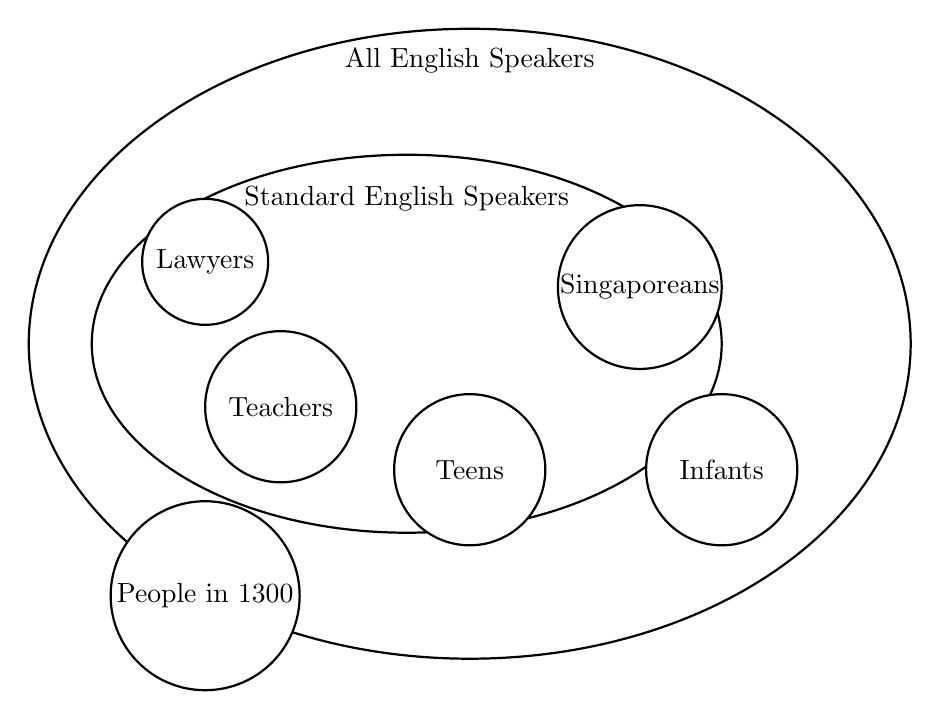
\begin{tikzpicture}[scale=0.8]
    % Main ellipse for all English speakers
    \draw[fill=white, thick] (0,0) ellipse (7cm and 5cm);
    \node at (0,4.5) {All English Speakers};
    
    % Ellipse for Standard English speakers
    \draw[fill=white, thick] (-1,0) ellipse (5cm and 3cm);
    \node at (-1,2.3) {Standard English Speakers};
    
    % Smaller ellipses for different groups
    \draw[fill=white, thick] (-3,-1) circle (1.2cm);
    \node at (-3,-1) {Teachers};
    
    \draw[fill=white, thick] (0,-2) circle (1.2cm);
    \node at (0,-2) {Teens};
    
    \draw[fill=white, thick] (2.7,0.9) circle (1.3cm);
    \node at (2.7,0.9) {Singaporeans};
    
    \draw[fill=white, thick] (4,-2) circle (1.2cm);
    \node at (4,-2) {Infants};
    
    \draw[fill=white, thick] (-4.2,1.3) circle (1cm);
    \node at (-4.2,1.3) {Lawyers};
    
    \draw[fill=white, thick] (-4.2,-4) circle (1.5cm);
    \node at (-4.2,-4) {People in 1300};
    
\end{tikzpicture}
\caption{Relationship among groups of English speakers (not to scale).}
\label{fig:speaker_groups}
\end{figure}


When it comes to the meaning\is{meaning!context-dependent|(}, there can often be layers and layers, any of which need to match the construction used to convey them. \textit{Try it and you'll regret it} has literal meaning\is{meaning!literal vs implied}: an instruction to try something followed by a predication that the experience will lead to regret. In everyday speech, though, it has a conditional meaning: `if you try it, you'll regret it'. On top of those, it also may carry an implied threat: `if you do that, I will punish you'. Here, the literal meaning of imperative \textit{try it} is turned on its head and comes to mean `don't try it'.

Sometimes old constructions pair with new meanings. That's how we ended up with the \textit{going to} future-time idiom: it began literally meaning going somewhere to do something (e.g., \textit{Why am I going there? I'm going to shop.}), but the fact that the activity could only happen after some period of travel time provided the opportunity for it to take on a futurate meaning. Other times grammatical constructions becomes less grammatical or falls out of use. Take the way we make questions and negatives in English, for instance. Shakespeare would have asked \textit{know you not?} instead of \textit{don't you know?}, and obviously, that's not how you and I say it.



So when do we say something's ungrammatical? A few situations come to mind. First, when the form doesn't pair with or even suggest any meaning at all, like \textit{Can the have running?} Second, when there's a mismatch between what you mean and what people expect you to mean. \textit{I have 12 years} is a perfectly good way of replying to the question \textit{How long do you have until retirement?} but it's ungrammatical\is{ungrammaticality!conditions for|(} in response to the question \textit{How old are you?}


Third, when you've got contradictory form--meaning pairs\is{form--meaning!pairing!contradictory} in the same utterance. \textit{I have two job} tells us both that that number of jobs is plural and that it's singular. And finally, when there's a strongly preferred alternative form, and there's no good reason not to use it.

Take a common phrase like \textit{It's very good}. Most English speakers would call this grammatical. Say \textit{It very good} instead, and you'll still get your meaning across~-- after all, ungrammatical doesn't mean meaningless. But listeners might pause, wondering why you skipped the verb. Maybe you're quoting something? Referencing a meme? Without a clear reason for the unusual form, they're likely to judge it ungrammatical.

These judgments aren't always reliable guides. Our brains sometimes flag perfectly grammatical sentences as wrong just because they're tricky to process. Other times, we breeze right past actually ungrammatical phrases without noticing, especially in casual conversation when we're focused on meaning rather than form.

This model frames grammaticality not as following rules from grammar books but as being about using form-meaning pairs that work for your linguistic community in a given context\is{context!and grammaticality|(}. Grammar isn't hardwired into our brains~-- despite what many linguists since the 1950s have claimed.\footnote{For example, we don't have innate principles and parameters the way \citet{chomsky1981lectures} claimed.} Language is fluid, shaped by its speakers. What counts as grammatical shifts across time, space, and social groups.

Most learners aim their speech at the Standard English-speaking world. Not everyone needs or wants to match these standards exactly. Many just want to communicate effectively~-- maybe to do business in a country like Vietnam. When students pursue Standard English, we guide them toward that goal. Fortunately, unlike rigid technical standards, language standards\is{language standard!flexibility of|(} bend without breaking. You can diverge quite a bit while still making perfect sense.

Grammar alone doesn't determine how language works. Social expectations and values cast long shadows, quietly shaping what people consider ``correct''. And this brings us to normativity~-- how social rules ripple through language, shaping both our words and our place in the world\is{intuition!fallibility of|)}\is{form--meaning!pairing|)}\is{meaning!context-dependent|)}\is{ungrammaticality!conditions for|)}\is{context!and grammaticality|)}\is{language standard!flexibility of|)}\is{grammaticality!model of|)}.

\section{Normativity}\label{sec:normativity}

A normative statement is one that deals not with how things are but how they ought to be, or how it is appropriate for them to be given some set of values\is{normativity!definition|(}.

\begin{table}[ht]
    \centering
        \begin{tabularx}{\textwidth}{|X|X|}
            \hline
            \textbf{Normative} & \textbf{Positive} \\
            \hline
            the rules of table manners & the claims of physics \\
            ethics & number theory \\
            economics: how we should distribute scarce resources & economics: how we actually distribute scarce resources \\
            language teaching & linguistics \\
            \hline
        \end{tabularx}
\end{table}

Geoff \textcite[205]{Pullum2019} makes the following normative observations:
\begin{itemize}[noitemsep]
    \item ``It is not polite to lick your knife'' offers a reason for not licking your knife;
    \item ``Torturing children is wrong'' implies a reason for not torturing children;
    \item ``Bach's music is beautiful'' suggests a reason for planning to attend a Bach concert;
    \item ``Inflation is too low'' signals to central bankers that they should lower interest rates;
    \item From ``the fact that torturing a child is immoral,'' it follows that we ought not to torture a child.
\end{itemize}

Are the rules of English grammar normative? And, if so, what can be learned from them about how folks ought to speak English? Pullum observes:
\begin{itemize}[noitemsep]
    \item Since nobody is under any obligation to speak English, in general, nothing at all follows concerning what anyone ought to do or not do.
    \item If we want to be taken to be speaking a particular variety of English, then we ought to follow the rules of that variety.
\end{itemize}

On the other hand, if we merely want to communicate with an English speaker, then what we ought to do is less clear.

\begin{itemize}[noitemsep]
    \item Perhaps, we ought to aim to be comprehensible\is{comprehensibility} or to be able to comprehend. Grammatical accuracy does not guarantee comprehensibility and ungrammatical language can be comprehensible, as we've seen, but most comprehensible English is also grammatical.
    \item Similarly, perhaps, we ought to be timely and fluent, but concern about being grammatical may reduce timeliness and fluency.
\end{itemize}

\subsection{Audience}

I would like to make one last point about normativity, which is that it often presumes a population within which the norm applies (recall Figure \ref{fig:speaker_groups}). If grammaticality is a combination of meaning, expectedness, and processability, for a particular group of speakers in a particular situation, then we really need to take account of not only who the speaker is but who the audience\is{audience|(} is. That audience is a key piece here, and, when it comes to learning English, the audience is often the social group of Standard English speakers.

This may not always be the case though. Some people learning English may wish to communicate with other non-native speakers, or with a specific cultural group, or perhaps even just within their own personal networks, and these groups may not be speakers of Standard English. For these folks, the norms of Standard English may be less relevant, and they may instead need to master a different set of linguistic norms~-- those that are relevant and meaningful within their specific target audience. But to the extent that our students wish to become speakers of Standard English, it seems clear to me that we, as language teachers, should facilitate that. And yet, even for those students, time should most likely not be spent grasping for finer and finer levels of Standard English fidelity instead of \hyperref[ch:vocabulary]{learning more vocabulary} or \hyperref[ch:fluency]{increasing their processing fluency}. 

As noted above, unlike technology standards, which often require high fidelity, language standards are quite forgiving within a language, as long as we are. And so English-language learners can often communicate\is{communication!and grammaticality} highly successfully while diverging significantly from the standards of their audience. As Vivian Cook observed, ``people cannot be expected to conform to the norm of a group to which they do not belong, whether groups are defined by race, class, sex, or any other feature. People who speak differently from some arbitrary group are not speaking better or worse, just differently'' \citep[194]{Cook1999}. The difficulty will be in how differently they speak, how much they wish to belong, and how much we wish to accept them.

Finally, facilitation can go two ways. The standard way is to put the burden on students to conform. That's how most English teachers see our jobs, and it's probably our most central role. But there is another way, and that is to help Standard-English speakers to accommodate\is{accommodation!by Standard English speakers}, include, accept, and welcome users of other varieties of English. Needless to say, language teachers typically do much less of this~-- many of us none at all. But, as English-language teachers, we should at least be aware of the possibility\is{normativity!definition|)}\is{audience|)}.

\section{Conclusion}

Throughout this chapter, we've grappled with issues that lie at the heart of English language teaching but that many TESL course never touch on. We've seen that \textit{standard} doesn't necessarily mean `best', that Standard English is more of a cluster of dialects than a monolithic entity, and that grammaticality is a complex concept that often defies simple rules.

These insights have significant implications for our practice as language teachers. For one, they should make us wary of oversimplification. When a student asks if something is ``correct'', often the answer is clear, but sometimes ``it depends'' might be better than a simple yes or no. We need to consider the context\is{context!and meaning}, the audience\is{audience!and grammaticality|(}, and the purpose of the communication.

At the same time, we can't ignore the reality that many of our students want to learn Standard English because of its social and economic currency. Our job, then, is to navigate a delicate balance: teaching the forms that will give our students access to certain opportunities, while also fostering an understanding of linguistic diversity and the validity\is{dialect!validity of} of different varieties of English.

This doesn't mean abandoning grammar instruction or letting ``errors'' slide. Rather, it means approaching these aspects of language teaching with a more nuanced understanding. Instead of simply labeling utterances as right or wrong, we can discuss how they might be perceived by different audiences, or how they align with the expectations of various contexts. It sometimes means talking about why we use a form and not just saying, ``here's the form we use.''

Ultimately, this chapter should leave you with more questions than answers~-- not a bad thing if you ask me. As language teachers, we're not just transmitting a set of rules, but helping our students navigate a complex linguistic landscape. The more we understand about the nature of that landscape~-- its standards, its varieties, its norms, and its ever-shifting boundaries~-- the better equipped we'll be to guide our students through it.

This isn't always an easy task. It requires ongoing learning and adaptation on our part. But it's this complexity that makes language teaching such a rich and challenging field. As we move forward to explore more specific aspects of English grammar and usage, keep these broader concepts in mind. They'll inform everything from how we explain a particular grammar point to how we respond to a student's non-standard usage\is{standard|)}\is{Standard English|)}\is{Standard English|)}\is{grammaticality|)}\is{normativity|)}\is{audience!and grammaticality|)}\is{shibboleth|)}.
\newpage

\section{Glossary of Key Terms}
\begin{description}
    \item[Standard English] The most widely accepted variety of a language, particularly in formal, educational, and professional contexts. Not inherently superior to other varieties, but backed by social and institutional power. See Section \ref{sec:standard}.
    
    \item[Standard Englishes] The various regional and national varieties of Standard English (e.g., Standard Canadian English, Standard British English), acknowledging that what counts as standard varies across regions while maintaining mutual intelligibility. See Section \ref{sec:standard}.
    
    \item[grammaticality] The degree to which a construction conforms to the accepted form--meaning pairings of a specific language community, reflecting regularities in syntax, morphology, and socio-cognitive norms, and regardless of how unconventional the meaning is. See Section \ref{sec:questioning-grammaticality}.
    
    \item[shibboleth] A linguistic feature that distinguishes members of one social group from another, often used (consciously or unconsciously) as a test of belonging. From Hebrew \textit{šibbōleṯ}. See Section \ref{sec:shibboleth}.
    
    \item[form-meaning pairing] The connection between how something is said (its linguistic form) and what it means in a particular context. Grammaticality often depends on using established form-meaning pairs within a speech community. See Section \ref{sec:gramm-model}.
    
    \item[normativity] Claims about how language ought to be used, rather than descriptions of how it is used. Related to prescriptive grammar but broader in scope. See Section \ref{sec:normativity}.
    
    \item[code-switching] Alternating between languages or language varieties within a single conversation, typically reflecting changes in context or social dynamics. See Section \ref{sec:gramm-model}.
    
    \item[fallacy of monosemy] The mistaken belief that words have (or should have) only one "true" meaning. See Section \ref{sec:monosemy}.
\end{description}

\noindent Note: Terms are cross-referenced to relevant sections where they are discussed in detail.



\begin{tcolorbox}[title=Exercises, colback=white]
    
\begin{enumerate}[noitemsep]
    \item Explain the concept of ``standard'' in the context of language. How is it different from the idea of ``good'' or ``correct''?
    \item Why is the distinction between Standard English and Standard English\uline{es} important?
    \item Provide an example of a shibboleth and explain how it functions as a social marker.
    \item What are some limitations of relying solely on intuition to determine grammaticality?
    \item The text argues that meaning is neither a necessary nor sufficient condition for grammaticality. Explain this claim with an example.
    \item What factors contribute to a form-meaning pairing being considered ``grammatical'' for a specific group of speakers in a particular situation?
    \item Describe a situation where an utterance might be considered ``ungrammatical'' even if it successfully conveys meaning.
    \item How can the concept of audience inform our understanding of grammaticality?
    \item What is meant by the term ``normative'' in the context of language?
    \item What is the role of a TESL teacher in navigating the complexities of Standard English and grammaticality for their students?
\end{enumerate}

\end{tcolorbox}

\begin{tcolorbox}[title=Answer key, colback=white]

\begin{enumerate}[noitemsep]
    \item ``Standard'' language is a set of widely accepted and institutionalized conventions, not quality or correctness. It's more about ubiquity and institutional backing than about being ``good'' or ``correct.''
    \item The distinction recognizes that ``Standard English'' is not one but a cluster of dialects with subtle variations across regions and cultures.
    \item A shibboleth is a linguistic feature that distinguishes a particular group of people. An example is the pronunciation of \textit{car} in various English dialects, where some pronounce it with a strong $langle$r$rangle$ sound, while others do not. It serves as a social marker, signaling belonging to a specific group.
    \item Intuition can be subjective and influenced by personal dialectal background. Also, complex grammatical structures or unfamiliar expressions can lead to incorrect judgments about grammaticality.
    \item \textit{Colorless green ideas sleep furiously} is grammatically well-formed, but it lacks meaningful content. Conversely, the utterance \textit{Go store} conveys meaning but is ungrammatical in Standard English.
    \item A form-meaning pairing is considered grammatical when it aligns with the shared linguistic conventions, expectations, and processing capabilities of a particular group in a given situation.
    \item \textit{Him and me seen it already.} would be considered ungrammatical many settings, even though its meaning is clear. The context and the audience's expectations influence perceptions of grammaticality.
    \item Different audiences have different expectations regarding language use. An utterance that might be acceptable among close friends may be considered ungrammatical in a formal presentation.
    \item \textit{Normative} statements are those about how language ``ought'' to be used based on established conventions or standards, rather than describing how it is actually used.
    \item TESL teachers need to guide students towards achieving communicative competence in Standard English while acknowledging the diversity of English dialects and fostering an understanding of language as a dynamic social phenomenon.
\end{enumerate}
\end{tcolorbox}

\begin{tcolorbox}[title=Essay Questions, colback=white]
    
\begin{enumerate}[noitemsep]
    \item Discuss the historical and social factors that have contributed to the emergence and dominance of Standard English. How has its role evolved over time?
    \item Critically evaluate the arguments for and against teaching Standard English to learners. Consider the potential benefits and drawbacks for students in different social and professional contexts.
    \item Analyze the relationship between grammaticality, meaning, and comprehensibility. Provide examples to illustrate how these concepts can sometimes align and sometimes diverge.
    \item Explore the concept of ``linguistic prejudice'' and discuss how it can manifest in attitudes towards non-standard dialects. How can language teachers promote respect for linguistic diversity?
    \item Consider the future of Standard English in a globalized world. How might factors such as technology, migration, and the rise of new Englishes influence its evolution and international role?
\end{enumerate}
\end{tcolorbox}
\chapter{Categories and functions: \\An overview} \label{ch:categories}

\epigraph{In the architecture of speech,\\
every beam must bear its load,\\
every word know its place,\\
and still the structure breathes.}{}

With some understanding of the concepts of standards, \is{Standard English!focus of book}Standard English(es), grammaticality, and normativity under our belts, I turn back to the ideas we started to develop in Chapter \ref{ch:1}. For the reasons laid out in Chapter 2, as well as for practical reasons, the focus will be on Standard English in Chapter 3 and most of the book. Here, I'll explain how \is{category, linguistic!vs function}categories and \is{function, syntactic!vs category}syntactic functions interact (Section \ref{sec:cat-funct}) in Standard English. I'll then provided explanations of the following categories: adjectives and adjective phrases in Section \ref{sec:adjs+adjPs}, pronouns in Section \ref{sec:pronouns}, and determinatives and determinative phrases in Section \ref{sec:DPs}.

\section{Categories and functions: An overview}\label{sec:cat-funct}
\subsection*{A garden metaphor}

I'm in my front garden in late May. The garden is lush, and the peonies are particularly notable as they begin to set their buds. Soon, they will bloom into large flowers. But a closer examination of their stems reveals that they aren't very thick or strong, despite being fairly long. In fact, these peonies grow to about three feet in height. Given the size of the blooms, which can rival that of a newborn's head, their slender stems often struggle to support the weight, and the flowers droop.

Stems play a crucial role in plants. They provide structural rigidity, ensuring the plant remains upright. In the case of these peonies, the stems might not be up to the task. But in the same garden, there's a rosebush. Its stems are sturdy and can easily support the weight of its flowers. While roses and peonies are different types (or \textsc{categories}) of plants, their stems serve a similar \textsc{function}: transporting nutrients and providing support.

But stems aren't the only plant parts with important roles. Consider the roots. While they anchor the plant into the ground, offering some structural support, their primary function is nutrient absorption. So, while roots prioritize nutrient absorption and offer some support, stems focus more on support while also aiding in nutrient transport.

In my garden, there's also a challenge with weeds, especially on the pathways. To combat this, I have spread mulch. Interestingly, it is made of wood, which functioned as a tree's ``stem'' (or trunk and branches). In its original role, the wood provided structural support to the tree and aided in nutrient transport. Now, repurposed as mulch, its function has shifted to weed suppression and moisture retention in the garden. Different organisms might see other uses for this wood: insects might view it as a food source, while a salamander might see it as a potential home.

The garden serves as a microcosm, illustrating the multifunctionality of natural elements. We categorize plant parts into stems, roots, flowers, and leaves, and each of these categories can serve multiple functions, from structural support to nutrient transport. Similarly, in language, words belong to lexical categories: nouns, verbs, adjectives, etc. These categories serve various linguistic functions, from modification to heading a phrase or acting as a subject or determiner.

The key takeaway is the flexibility and multifunctionality inherent in both nature and language. There isn't always a one-to-one relationship between categories and functions~-- a single function can be realized by multiple categories, just as a single category can fulfill various roles.

\subsection{Many-to-many relationships} \label{sec:many-to-many}
\is{many-to-many relationships!between categories and functions|(}To reiterate, there's no one-to-one relationship between \is{category, linguistic!many-to-many relationship with functions}categories and \is{function, syntactic!many-to-many relationship with categories}functions, and the belief that there is is akin to the \hyperref[sec:fallacy-of-monosemy]{fallacy of monosemy}\is{fallacy of monosemy}. If there were, then we would have a much easier time defining the categories. For instance, if nouns and only nouns functioned as subjects, then we could simply define a noun as any word that functions as a subject, and we wouldn't have to bother with the stuff about coming after \textit{the} and \textit{a}, adjective phrases as modifiers, plurals, and the rest of it (Section \ref{sec:nouns}). But that's not how language works.

This echoes the point that was being made in the soup sketch: no single criterion will define a category. And yet, assuming one-to-one relationships is more or less what \is{traditional grammar!conflation of categories and functions}traditional English school grammars have always tried to do. They say that an adjective is any word that modifies a noun. Here's an example from the 11th edition of the very popular \textit{The big blue book of grammar and punctuation} \citep{straus2014}.

\begin{quote}
    \begin{itemize}[noitemsep]
        \item A \textbf{noun} is a word or set of words for a person, place, thing, or idea (p.~1).
        \item An \textbf{adjective} is a word or set of words that \textbf{modifies} (i.e., describes) a noun or pronoun. Adjectives may come before the word they modify (p.~15).
    
        \textit{\textbf{Examples}:}
        \begin{itemize}[noitemsep]
            \item \textit{That is a \textbf{cute} puppy.}
            \item \textit{She likes a \textbf{high school} senior.}
        \end{itemize}
    \end{itemize}
\end{quote}
    
Of course, this can't be right. A high school is a place (or a thing?), which should make \textit{high school} a noun under the definition above, but in the example sentence, it's supposed to be an adjective. In other cases, such as \textit{the Trudeau government}, Trudeau is a person but the word is, in the phrasing of \textit{The blue book of grammar and punctuation}, ``modifying the noun'' \textit{government}. So is \textit{Trudeau} a noun or an adjective? Or is it in some kind of quantum superposition of being both at the same time? In fact, both \textit{high school} and \textit{Trudeau} are just nouns, full stop (check the properties in Section \ref{sec:nouns} yourself if you doubt this).

This illustrates how we can better understand language by recognizing that the relationships between categories (like noun and adjective) and functions (like subject or modifier) are many-to-many. \is{traditional grammar!category mistake in}Traditional grammars often try to resolve this complexity with explanations like "it's a noun functioning as an adjective," but that's like saying that the woody stem of a rhododendron is ``functioning as a rose stem,'' or that poppies' long, slender stems ``function as peony stems.'' These stems all function as (better or worse) supports, but the only stem that ``functions as a rose stem'' is a rose stem. Claiming that a noun ``functions as an adjective'' is a \is{category mistake!defined}category mistake: \textsc{adjective} is not a function.

So to be perfectly clear, almost all categories perform multiple functions, and almost all functions can be performed by more than one category. Noun phrases, being no exception, have multiple functions, and not every subject is a noun phrase. In fact, it's quite common for nouns to function as modifiers in NPs as \textit{Trudeau} does in \textit{the Trudeau government}.

Make a list of other noun–noun combinations (e.g., \textit{soccer ball}, \textit{faculty office}), where the first is a modifier and the second is the head, and then check the following examples.

\begin{itemize}[noitemsep]
    \item \textit{health care}, \textit{world war}, \textit{law enforcement}, \textit{climate change}, \textit{air force}, \textit{family member}, \textit{video clip}, \textit{credit card}, \textit{breast cancer}, \textit{interest rate}, \textit{justice department}, \textit{tea party}, \textit{blood pressure}, \textit{Saturday night}, \textit{security council}, \textit{heart attack}, \textit{task force}, \textit{press conference}, \textit{stock market}, \textit{school district}, \textit{death penalty}
    \item \textit{cell phone}, \textit{phone call}, \textit{call centre}, \textit{centre stage}, \textit{stage manager}, \textit{manager position}, \textit{position paper}, \textit{paper towel}, \textit{towel rack}
    \item \textit{community college}, \textit{college student}, \textit{student loan}, \textit{loan guarantee}, \textit{guarantee program}, \textit{program director}, \textit{director level}, \textit{level change}
\end{itemize}\is{many-to-many relationships!between categories and functions|)}

\subsection{Categories}

\is{category, linguistic!defined}We have two fundamental types of categories: \textsc{lexical categories} and \textsc{phrasal categories}. These categories can often be identified out of context. For instance, if you see the word \textit{happy}, you can categorize it as an adjective. You can look it up in a dictionary, and it will say ``adjective''. There is no need for any more context. In some cases, the category will be ambiguous, as we saw with verbs/nouns like \textit{run}, \textit{jump}, and \textit{walk} in Section \ref{sec:verbs}. It's not the case that each of these words belongs to two categories; the verb \textit{walk} and the noun \textit{walk} are different words, belonging to different lexical categories. It's simply the case that we may not have enough information to say which of the two words we're looking at in a particular case. It is clear, however, that \textit{walk} is not an adjective, adverb, preposition, or anything other than a noun or a verb.

\textsc{Functions}, on the other hand, are relational. \is{function, syntactic!relational nature of}We can't ever look up a word in a dictionary and find out whether it's a modifier, a subject, a head, or a dependent. These function can only be determined in a context by seeing how the phrases relate to those around them.

\subsubsection*{Lexical categories}

\is{category, linguistic!lexical vs phrasal}\textsc{Lexical categories} contain individual words. Usually, in English, these are set off by spaces in writing, although there are some words that contain an internal space (e.g., \textit{each other}). So far, we have considered nouns and verbs. The other lexical categories we will look at in this book are adjectives, pronouns (a kind of noun), determinatives, prepositions, adverbs, coordinators, and subordinators. The only lexical category we won't eventually look at is interjections.\footnote{If you'd like to learn about them, I suggest starting with the Wikipedia entry for English interjections, for which, as of this writing, I am the primary author: \href{https://en.wikipedia.org/wiki/English\textunderscore interjections}{https://en.wikipedia.org/wiki/English\textunderscore interjections}.}

\subsubsection*{Phrasal categories}

Most of the lexical categories mentioned so far have a related phrasal category, as shown in Figure \ref{fig:projections}. For nouns, there are noun phrases (or NPs); for verbs there are VPs; for adjectives, AdjPs, etc. There's one additional phrasal category, clause, which is headed by a VP as we saw in Section \ref{sec:verbs}.\is{determinative, determinative phrase (DP)}\is{noun, noun phrase (NP)}\is{verb, verb phrase (VP)}\is{adverb, adverb phrase (AdvP)}\is{preposition, preposition phrase (PP)}\is{adjective, adjective phrase (AdjP)}\is{clause}


\begin{figure}[h]
    \centering
    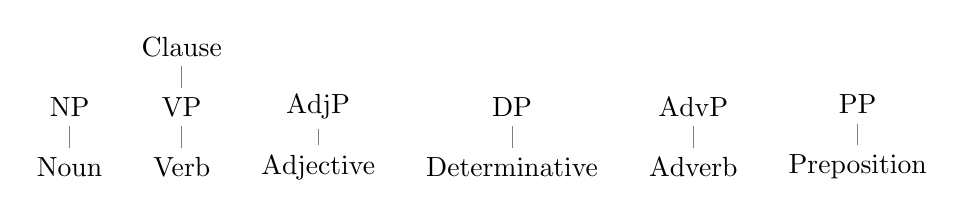
\begin{tikzpicture}[node distance=0.4cm]
        % Lexical row
        \node (noun) {Noun};
        \node[right=of noun] (verb) {Verb};
        \node[right=of verb] (adj) {Adjective};
        \node[right=of adj] (det) {Determinative};
        \node[right=of det] (adv) {Adverb};
        \node[right=of adv] (prep) {Preposition};
        
        % Phrasal row
        \node[above=of noun, anchor=base] (np) {NP};
        \node[above=of verb, anchor=base] (vp) {VP};
        \node[above=of adj, anchor=base] (adjp) {AdjP};
        \node[above=of det, anchor=base] (detp) {DP};
        \node[above=of adv, anchor=base] (advp) {AdvP};
        \node[above=of prep, anchor=base] (prepP) {PP};
        
        % Top row for Clause
        \node[above=of vp, anchor=base] (clause) {Clause};
        
        % Draw the light vertical lines
        \draw[gray, thin] (noun) -- (np);
        \draw[gray, thin] (verb) -- (vp);
        \draw[gray, thin] (adj) -- (adjp);
        \draw[gray, thin] (det) -- (detp);
        \draw[gray, thin] (adv) -- (advp);
        \draw[gray, thin] (prep) -- (prepP);
        \draw[gray, thin] (vp) -- (clause);
    \end{tikzpicture}
    \caption{Some lexical and phrasal categories}
    \label{fig:categories}
\end{figure}\label{fig:projections}

As we saw in chapter 1, the everyday meaning of \textit{phrase} happens to be ``a group of words that have a particular meaning when used together,'' but for our purposes, all we need is a head word. Often, this comes with dependents, but one-word phrases are also possible. This is another example of the difference between the everyday meaning and the technical definition. So, here, \textit{go to school} is a \textsc{VP}, but so is \textit{go} in \textit{please, go}. We can have a long NP such as \textit{all the very interesting people who I met yesterday}, but we can also have single-word NPs such as \textit{they} or \textit{water}.

\subsection{Syntactic functions}

\is{function, syntactic!defined}\textsc{Syntactic functions} (or just \textsc{functions}) are broadly split into \textsc{Head} and \textsc{Dependent}. There is only one kind of head, but we'll divide dependents into \textsc{Subject}, \textsc{Modifier}, \textsc{Determiner}, and \textsc{Complement}. We'll also include a special kind of complement called an \textsc{Object}. \is{function, syntactic!list of}There are some other functions that I'll introduce later, but we'll stick with these for now.

Once again, the following explanations may include terms that you're not yet familiar with. As I've said, because this is a system, this is difficult to avoid, but the terms will be explained soon, at which point, you may wish to review these definitions.

\subsubsection*{Head}\label{sec:head}

\is{head (function)}The head is the function of the most important element in a phrase. The phrase is almost always named after the lexical category of its head (e.g., an AdjP has an adjective as its head), and every phrase has a head. Heads are often the only element in a phrase. For instance, in \textit{rain fell}, the subject NP contains just the head noun \textit{rain} and the head VP contains just the head verb \textit{fell}.

I will often shorten \textsc{Head} to H.

\subsubsection*{Dependent}\label{sec:Dep}

\is{dependent (Dep)!defined}A dependent is any element in the structure of a phrase or clause other than the head: \textit{\uline{the} \uline{best} kind} (NP headed by \textit{kind} with two dependents); \textit{won \uline{an award}} (VP headed by \textit{won} with one dependent); \textit{\uline{more} important} (AdjP headed by \textit{important} with one dependent). Subjects, complements, modifiers, and determiners are all kinds of dependents.

I will often shorten \textsc{Dependent} to Dep.

\paragraph*{Subject} \label{sec:subjects} (a type of Dependent)

\begin{itemize}[noitemsep]
    \item \is{subject (Subj)!defined}The subject typically functions as the topic of the clause and is syntactically a dependent of the VP in a clause.
    \item It most often precedes the VP in declarative clauses (e.g., \textit{\uline{A sunny day}} [\textit{should be savoured}]).
    \item In questions with subject--auxiliary inversion, the subject follows the auxiliary (e.g., \textit{Could \uline{they} be right?}), a structure further explored in Section \ref{sec:basic-int}.
    \item Semantically, the subject often denotes the agent in active sentences, but this is not universally the case, setting the stage for exceptions discussed in Section \ref{sec:subjects2}.
    \item \is{agreement!subject--verb}Agreement with the verb in person and number is a key characteristic of the subject, particularly visible in present tense verbs (e.g., \textit{I like it} vs \textit{She like\uline{s} it}).
    \item While typically an NP, subjects can also be clauses, VPs, or even preposition phrases (PPs), highlighting the flexibility of this grammatical function.
\end{itemize}


I will often shorten \textsc{Subject} to Subj.

\paragraph*{Determiner} \label{sec:determine} (a type of Dependent)

\begin{itemize}[noitemsep]
    \item \is{determiner (Det)!defined}Determiners are found only in NPs.
    \item A Head noun will never have more than one determiner \\(e.g., \textit{*\uline{my} \uline{the} class}).
    \item Determiners are usually determinative phrases (DPs) or possessive NPs \\(e.g., \textit{the}, \textit{almost all}, \textit{ some},\textit{ each},\textit{ my},\textit{ Brett's}).
    \item A singular countable noun needs a determiner to form an NP \\(e.g., \textit{I need a}/\textit{the}/\textit{each}/\textit{every pen}, but not \textit{*I need pen}).
    \item Determiners come before modifiers in the NP \\(e.g., \textit{\uline{the} Trudeau government}).
\end{itemize}

I will often shorten \textsc{Determiner} to Det. \textsc{Determin\uline{er}} and \textsc{modifi\uline{er}} are syntactic functions. The \textit{--er} tells you it's a function. In contrast, \textsc{Determina\uline{tive}} and \textsc{adjec\uline{tive}} are lexical categories.

\paragraph*{Modifier} \label{sec:modifier}(a type of Dependent)

\begin{itemize}[noitemsep]
    \item \is{modification, modifier!defined}Most heads allow one or more modifiers.
    \item Typical modifiers are AdjPs and AdvPs, but almost any phrase can be a modifier.
    \item Modifiers can often move position \\(e.g., \textit{he \uline{quickly} jumped the fence}, \textit{he jumped the fence \uline{quickly}}).
    \item Modifiers can often be removed without drastic or unexpected changes of meaning (e.g., \textit{a \uline{nice, furry} dog was sitting there} $\rightarrow$ \textit{a dog was sitting there}).
    \item Similarly, modifiers can almost always be added or removed without affecting grammaticality.
    \item In theory, the number of modifiers is unlimited.
    \item Unfortunately, the boundary between complements and modifiers can be very fuzzy.
\end{itemize}

I will often shorten \textsc{Modifier} to Mod.

\paragraph*{Complement} \label{sec:complement}(a type of Dependent)

\begin{itemize}[noitemsep]
    \item \is{complement, complementation!defined}Complements ``complete'' a phrase. This meaning is reflected in the spelling \textit{compl\uline{e}ment}. (\textit{Compl\uline{i}ments}, in contrast, are nice things you say about somebody.)
    \item Almost any kind of phrase can be a complement, though AdvP and DP complements are very rare.
    \item Complements usually follow their head. In contrast, modifiers can often move around (e.g., the modifier \textit{quickly} can go at the beginning, middle, and end of \textit{she changed direction}).
    \item Complements are ``selected'' by a head \\(e.g., \textit{listen \uline{to the music}} not \textit{*listen \uline{about the music}}; \textit{listen} selects a \textit{to} PP.).
    \item If a phrase is indifferent about a head, it's not a complement. For example, \textit{on Monday} can go with almost any verb \\(e.g., \textit{eat}/\textit{play}/\textit{work}/\textit{think}/\textit{sit \uline{on Monday}}).
    \item There are zero, one, two, or sometimes three complements, but never four.\footnote{If you think of subjects as a kind of complement, then four is possible.}
    \item Unfortunately, the boundary between complements and modifiers can be very fuzzy.
\end{itemize}

I will often shorten \textsc{Complement} to Comp.

\paragraph*{Object} \label{sec:object} (a type of Complement)

\begin{itemize}[noitemsep]
    \item \is{object (Obj)!defined}Objects are a kind of complement.
    \item Objects are always dependents in VPs or in PPs \\(e.g., \textit{grab \uline{the bag}} or \textit{in \uline{the bag}}).
    \item Objects are almost always NPs.
    \item If there's an action, the object is usually what is acted upon \\(e.g., \textit{I threw \uline{the ball}).}
    \item The object of an active sentence is usually the subject of the related passive sentence (e.g., \textit{A friend made \uline{the cake}} $\rightarrow$ \textit{\uline{the cake} was made by a friend}).
    \item Verbs like \textit{be},\textit{ become},\textit{ seem},\textit{ appear},\textit{ feel} (e.g., \textit{I feel good}), \textit{look} (e.g., \textit{it looks easy}), etc. take complements, but not the special kind called objects.
\end{itemize}

I will often shorten \textsc{Object} to Obj.

\begin{tcolorbox}[title=Exercises, colback=white]
    Underline the whole subject in each quotation. If there is more than one subject, underline the first two. Ignore any further subjects.
    \begin{enumerate}[noitemsep]
        \item ``Undressing her was an act of recklessness, a kind of vandalism, like releasing a zoo full of animals, or blowing up a dam.'' \phantom{xxxxxxxxxxxxxx} \hfill--Michael~Chabon
       \item ``The war in Zagreb began over a pack of cigarettes.''\hfill--Sara Nović
       \item ``Jack put his arm out the window, waving his hat like a visiting dignitary, backed into the street, and floated away, gentling the gleaming dirigible through the shadows of arching elm trees, light dropping on it through their leaves like confetti as it made its ceremonious passage.'' \phantom{xxxxxxxx} \hfill--Marilynne~Robinson
     \item ``A sudden warm rainstorm washes down in sweet hyphens.''\phantom{xxxxxxxx} \hfill--J.~M.~Ledger
     \item ``And as the ax bites into the wood, be comforted in the fact that the ache in your heart and the confusion in your soul means that you are still alive, still human, and still open to the beauty of the world, even though you have done nothing to deserve it.''\hfill--Paul Harding
     \item ``Within seconds of that thought, the train entered Washington, where she was to come to her end more than sixty-eight years later, a mother to seven living and two dead, a grandmother to twenty-one living and three dead, a great-grandmother to twelve, a great-great grandmother to twins.''\hfill--Edward~P.~Jones
     \item ``We were all a little drunk with spring, like the fat bees reeling from flower to flower, and a strange insurrectionary current ran among us.''\hfill--Tobias Wolff
     \item ``When he was dry, he believed it was alcohol he needed, but when he had a few drinks in him, he knew it was something else, possibly a woman; and when he had it all~-- cash, booze, and a wife~-- he couldn't be distracted from the great emptiness that was always falling through him and never hit the ground.''\hfill--Denis Johnson
     \item ``Lizards skit like quick beige sticks.''\hfill--Richard Beard
    \end{enumerate}
\end{tcolorbox}
\newpage
\begin{tcolorbox}[title=Answer key, colback=white]

\begin{enumerate}[noitemsep]
    \item \textit{Undressing her}
    \item \textit{The war}
    \item \textit{Jack} \dots \textit{ it}
    \item \textit{A sudden warm rainstorm}
    \item \textit{the ax \dots~the ache in your heart and the confusion in your soul} 
    \item \textit{the train \dots~she}
    \item \textit{We \dots~a strange insurrectionary current}
    \item \textit{he \dots~he}
    \item \textit{Lizards}
\end{enumerate}
\end{tcolorbox}

\section{Adjectives and adjective phrases}\label{sec:adjs+adjPs}

Now that you have a better understanding of categories and verbs, it's time to look at the characteristics of \is{adjective, adjective phrase (AdjP)!characteristics of}adjectives and \is{adjective, adjective phrase (AdjP)!characteristics of}adjective phrases.

Before we start, I think it's useful to restate that these characteristics are often related to teaching points. For example, the issue of nouns being countable is actually an issue that causes a great deal of confusion for students. So, with that said, \dots

\begin{enumerate}[noitemsep]
    \item \is{adjective, adjective phrase (AdjP)!denotation of (properties, characteristics)}Adjectives typically denote properties or characteristics, but not objects or actions.
    \item \is{adjective, adjective phrase (AdjP)!head}Adjectives always head adjective phrases.
    \item \is{adjective, adjective phrase (AdjP)!as modifier (in NP and AdjP)}Adjective phrases typically function as modifiers in NPs (\textit{a \uline{nice} day}) and \is{adjective, adjective phrase (AdjP)!as complement (in VP and PP)}complements in VPs (\textit{was \uline{nice}}). Sometimes they also function as modifiers in AdjPs, though not in VPs or most other phrase types, and complements in PPs (\textit{for \uline{free}}).
    \item \is{adjective, adjective phrase (AdjP)!tests for (complement to \textit{be}, \textit{become}, \textit{seem})}Any phrase that can function as complement to all three of \textit{be}, and \textit{become}, and \textit{seem} is an adjective phrase.
    \item \is{adjective, adjective phrase (AdjP)!tests for (modification by very, too, so)}Any word that can be modified by all three of \textit{very}, and \textit{too}, and \textit{so} is an adjective (or an adverb).
    \item \is{adjective, adjective phrase (AdjP)!gradability of (-\textit{er}/-\textit{est}, \textit{more}/\textit{most})}Many adjectives can take \textit{--er} and \textit{--est} endings, but so can a number of commonly used adverbs.
    \item Many adjectives can be gradable with \textit{more} and \textit{less}, and \textit{most} and \textit{least}, but so can many adverbs.
    \item \is{adjective, adjective phrase (AdjP)!formation of adverb from (-\textit{ly})}Many adjectives can take an \textit{--ly} ending and become an adverbs.
\end{enumerate}

Here are some examples.

\subsection*{Denotation}

As in Section \ref{sec:nouns}, the terms used here are just everyday descriptions. They're not technical terms, nor are they meant to be exhaustive.

\begin{itemize}[noitemsep]
    \item \textbf{evaluative properties:} \textit{good}, \textit{great}, \textit{helpful}, \textit{interesting}
    \item \textbf{scalar properties:} \textit{big}, \textit{heavy}, \textit{high}, \textit{old}, \textit{thick}
    \item \textbf{relationship properties:} \textit{Canadian}, \textit{different}, \textit{mutual}, \textit{ninth}, \textit{other}
    \item \textbf{material properties:} \textit{ceramic}, \textit{metallic}, \textit{plastic}, \textit{wooden}, \textit{woolen}
    \item \textbf{state properties:} \textit{amorphous}, \textit{aqueous}, \textit{crystalline}, \textit{gaseous}, \textit{viscous}
    \item etc.
\end{itemize}

\subsection*{Heading adjective phrases}
\begin{itemize}[noitemsep]
    \item \textit{\uline{happy}}, \textit{very \uline{happy}}, \textit{very \uline{happy} with the outcome}
    \item \textit{\uline{nice}}, \textit{not \uline{nice}}, \textit{no \uline{nicer} than the other one}
    \item \textit{\uline{interesting}}, \textit{easily more \uline{interesting} than mine}
    \item \textit{slightly too \uline{big}}
\end{itemize}

\subsection*{AdjPs as modifiers in NPs}
\begin{itemize}[noitemsep]
    \item \uline{\textit{civil}} \textit{rights}, \textit{some \uline{quite good} news},  \uline{\textit{national}} \textit{security}, \textit{the \uline{whole} thing}, \uline{\textit{recent}} \textit{years}, \textit{our \uline{mental} health}, \textit{her \uline{very best} friend}, \textit{a \uline{really big} deal}, \textit{a \uline{supremely important} responsibility}
\end{itemize}

\subsection*{AdjPs as complements to \textit{be}, \textit{become}, and \textit{seem}}
\begin{itemize}[noitemsep]
    \item \textit{is}/\textit{became}/\textit{seems} \textit{clear},  \textit{aware}, \textit{available}, \textit{pregnant},  \textit{familiar to me},  \textit{popular with the ladies}, and \textit{very interested in the difference}
\end{itemize}

\subsection*{AdjPs with \textit{very}, \textit{too}, and \textit{so} as modifiers}
\begin{itemize}[noitemsep]
    \item \textit{very}/\textit{too}/\textit{so} \textit{good}, \textit{important}, \textit{late}, \textit{different}, \textit{difficult}, and \textit{nice}
    \item(Many adverbs work here too: \textit{well}, \textit{importantly}, \textit{differently}, \textit{nicely})
\end{itemize}

\subsection*{Taking \textit{--er} and \textit{--est} suffixes}
\begin{itemize}[noitemsep]
    \item \textit{bigger}, \textit{biggest}; \textit{greater}, \textit{greatest}; \textit{older}, \textit{oldest}; \textit{lower}, \textit{lowest}; \textit{yonger}, \textit{youngest}
    \item (A number of commonly used adverbs work here too: \textit{stay longer}, \textit{leave earlier}, \textit{run faster}, \textit{work harder}, \textit{jump higher})
\end{itemize}

\subsection*{Graded with \textit{more} and \textit{less}, and \textit{most} and \textit{least}}
\begin{itemize}[noitemsep]
    \item \textit{more}/\textit{less}/\textit{most}/\textit{least} \textit{likely}, \textit{expensive}, \textit{favourite}, \textit{important}, \textit{restrictive}, \textit{effective}, \textit{able}, \textit{possible}
    \item (Again, adverbs like \textit{frequently}, \textit{environmentally}, \textit{politically}, \textit{often}, etc. work here too)
\end{itemize}

\subsection*{Take \textit{--ly} to form adverbs}
\begin{itemize}[noitemsep]
    \item \textit{quick} $\rightarrow$ \textit{quickly}; \textit{real} $\rightarrow$ \textit{really}; \textit{actual} $\rightarrow$ \textit{actually}; \textit{probable} $\rightarrow$ \textit{probably}; \textit{final} $\rightarrow$ \textit{finally}; \textit{simple} $\rightarrow$ \textit{simply}; \textit{exact} $\rightarrow$ \textit{exactly}; \textit{certain} $\rightarrow$ \textit{certainly}
\end{itemize}

\subsection*{Exercise}
Apply the properties to identify the adjectives in this excerpt from ``A very old man with enormous wings'' by Gabriel García Márquez, translated by Gregory Rabassa. If you're not sure how to do this, have a look at the worked answers that follow.
\begin{quote}
On the following day, everyone knew that a flesh-and-blood angel was held captive in Pelayo's house. Against the judgment of the wise neighbor woman, for whom angels in those times were the fugitive survivors of a celestial conspiracy, they did not have the heart to club him to death. Pelayo watched over him all afternoon from the kitchen, armed with his bailiff's club, and before going to bed he dragged him out of the mud and locked him up with the hens in the wire chicken coop. In the middle of the night, when the rain stopped, Pelayo and Elisenda were still killing crabs. A short time afterward, the child woke up without a fever and with a desire to eat. Then they felt magnanimous and decided to put the angel on a raft with fresh water and provisions for three days and leave him to his fate on the high seas. But when they went out into the courtyard with the first light of dawn, they found the whole neighborhood in front of the chicken coop having fun with the angel, without the slightest reverence, tossing him things to eat through the openings in the wire as if he weren't a supernatural creature but a circus animal.
\end{quote}

\paragraph*{\textit{Following}}
\textit{On the \uline{following} day everyone knew that a flesh-and-blood angel was held captive in Pelayo's house.}

\begin{itemize}[noitemsep]
    \item \textit{Following} is a modifier in the noun phrase \textit{the following day}, but it is not modifiable by \textit{very}, \textit{so}, or \textit{too}.
    \item There is no \textit{more}/\textit{most}/\textit{less}/\textit{least following}.
    \item We cannot say something is \textit{the followingest}.
    \item There is no adverb \textit{followingly}.
    \item It cannot function as the complement of \textit{become} or \textit{seem} \\(e.g., \textit{the day became following}).
\end{itemize}
Therefore, \textit{following} is probably not an adjective, or at best it is a very bad example of an adjective. Since it ends in \textit{--ing} consider whether it might be a verb.

\paragraph*{\textit{Those}}
\textit{Against the judgement of the wise neighbor woman, for whom angels in \uline{those} times were the fugitive survivors of a celestial conspiracy, they did not have the heart to club him to death.}
\begin{itemize}[noitemsep]
    \item \textit{Those} comes before the noun \textit{times}, but it doesn't denote a property. Instead, it has a kind of pointing meaning.
    \item It is not gradable with \textit{--er}, \textit{more}, or \textit{less}.
    \item It cannot be modified by \textit{very}.
    \item It cannot function as complement of \textit{become} or \textit{seem}.
    \item There is no word \textit{*thosely}.
\end{itemize}
So, \textit{those} is probably not an adjective either.

\paragraph*{\textit{Wire}}
\textit{Pelayo watched over him all afternoon from the kitchen, armed with his bailiff's club, and before going to bed he dragged him out of the mud and locked him up with the hens in the \uline{wire} chicken coop.}

\begin{itemize}[noitemsep]
    \item \textit{Wire} functions as a modifier in the noun phrase \textit{the wire chicken coop}, but it denotes a physical object, not a property.
    \item We can say \textit{that seems like wire}, but not \textit{*that seems wire}.
    \item It has none of the other characteristics of an adjective.
    \item It can modify a verb (e.g., \textit{a \uline{wire wrapped} guitar string}).
\end{itemize}
Again, \textit{wire} is probably not an adjective. Given that it denotes a physical object, consider whether it might be a noun.

\paragraph*{\textit{Magnanimous}}
\textit{Then they felt \uline{magnanimous} and decided to put the angel on a raft with fresh water and provisions for three days and leave him to his fate on the high seas.}

\begin{itemize}[noitemsep]
    \item \textit{Magnanimous} doesn't modify a noun, but it functions as a complement in a VP headed by \textit{felt}.
    \item It denotes a characteristic of the people (they).
    \item There isn't a word \textit{*magnanimouser}, but we do have \textit{more} or \textit{less magnanimous}.
    \item It can be modified by \textit{very}.
    \item There is an adverb \textit{magnanimously}.
    \item There's nothing wrong with \textit{it seems magnanimous}.
\end{itemize}
So, \textit{magnanimous} seem to be an adjective.

\paragraph*{\textit{Fresh}}
\textit{Then they felt magnanimous and decided to put the angel on a raft with \uline{fresh} water and provisions for three days and leave him to his fate on the high seas.}

\begin{itemize}[noitemsep]
    \item \textit{Fresh} is a modifier in the noun phrase \textit{fresh water}.
    \item It denotes a scalar property.
    \item It can be graded (e.g., \textit{fresher}, \textit{freshest}, \textit{least fresh}).
    \item Something can be \textit{very fresh}.
    \item There is an adverb \textit{freshly}.
    \item Something can \textit{seem fresh}. And while it's kind of unusual for something to \textit{become fresh}, just because things tend to go from fresh to stale and not the other way around, there's no grammatical problem with \textit{become fresh}.
\end{itemize}
Clearly, \textit{fresh} is an adjective.

Now, have another look at the passage with these examples in mind.

\begin{tcolorbox}[title=Summary and review, colback=white]
    Fill in the gaps with \textit{noun}(\textit{s}), \textit{verb}(\textit{s}), or \textit{adjective}(\textit{s}).

    \phantom{a}

    \phantom{zzz}A word that denotes a person, place, or thing is a/an \uline{\hspace{1.5cm}}.
    \uline{\hspace{1.5cm}} It can typically follow \textit{the} or \textit{a}. A word that is countable is a/an \uline{\hspace{2cm}}.
    Almost every \uline{\hspace{2cm}} can follow the infinitive marker \textit{to}.
    A noun phrase is typically headed by a/an \uline{\hspace{2cm}}.
    An adjective phrase is always headed by a/an \uline{\hspace{2cm}}.
    \uline{\hspace{2cm}} phrases can perform a variety of functions, including subject and object. Any phrase that can function as complement to \textit{be}, and \textit{become}, \textbf{and} \textit{seem} is \\a/an \uline{\hspace{2cm}} phrase. Almost every \uline{\hspace{2cm}} has an \textit{--ing} form.
    \uline{\hspace{2cm}} commonly denote actions and states, and they do not denote physical objects.

    \phantom{zzz}Many \uline{\hspace{2cm}} can take \textit{--er} and \textit{--est} endings, but so can many adverbs.
    \uline{\hspace{2cm}} typically denote properties or characteristics, but not objects or actions.
    \uline{\hspace{1.4cm}}~phrases can typically be possessive. Typically,
    \uline{\hspace{2cm}} can be modified by adjective phrases. Many \uline{\hspace{2cm}} can take an \textit{--ly} ending and become an adverbs. Almost every \uline{\hspace{2cm}} has a third-person singular \textit{--s} form. A/an \uline{\hspace{2cm}} is often in an agreement relationship with a phrase functioning as its subject. A/an \uline{\hspace{2cm}} cannot be modified by an adjective phrase. The head of a clause is typically a/an \uline{\hspace{2cm}} phrase.
    \uline{\hspace{2cm}} can denote almost anything from objects to actions to characteristics.

    \phantom{zzz}Any word that can be modified by \textit{very}, \textit{too}, and \textit{so} is a/an \uline{\hspace{2cm}} (or an adverb).
    \uline{\hspace{2cm}} cannot typically be modified by adverb phrases. A word that has a past-tense form is a/an \uline{\hspace{2cm}}. Many \uline{\hspace{2cm}} can be gradable with \textit{less} and \textit{least}, and so can many adverbs.
    \uline{\hspace{2cm}} phrases modify nouns and \uline{\hspace{2cm}}, but not verbs. Almost any word that is plural is a/an \uline{\hspace{2cm}}.
    \uline{\hspace{2cm}} phrase must be headed by a verb.

    \phantom{a}

    \phantom{zzz}Keep working on recalling the properties of nouns and verbs, and add adjectives to your practice.
\end{tcolorbox}

\section{Pronouns, and determinatives and DPs}

\subsection{Pronouns}\label{sec:pronouns}
\begin{itemize}[noitemsep]
    \item Did you ever notice that we sometimes say things like, \textit{look at the baby. It's so cute}. but we'd never say, \textit{look at her boyfriend. *It's so cute}.
    \item Did you ever notice that plural \textit{they} is used to refer to anything from teachers to trees but singular \textit{they} is only for persons? If you doubt me, give it a try.
    \item Did you ever notice that in some uses, \textit{whose} is used to refer to anything from children to chambers (e.g., \textit{The chasm ran through a chamber whose ceiling was lost in the darkness above}), but \textit{who} is only for persons?
    \item Did you ever notice that in some cases \textit{which} can't be used for persons (e.g., *\textit{that's the guy which sold me the car})?
    \item Of course, everyone's aware of the masculine/feminine gender pronouns, but did you ever think about personal/non-personal gender pronouns?
\end{itemize}

\is{pronoun!defined}Pronouns are a special kind of noun. They typically refer to another noun phrase that has come before or that comes later (e.g., in \textit{Xi saw \uline{the egg} fall but caught \uline{it} before \uline{it} smashed}, the pronoun \textit{it} refers to the egg). There are only a small number of pronouns. The main ones are set out in Table \ref{tab:pronouns}.

\begin{sidewaystable}
\centering
\caption{The main pronouns in Modern English}
\label{tab:pronouns}
\begin{tabular}{l l l c c c c c}
\multicolumn{8}{c}{\textbf{Pronoun Forms}} \\
\hline
\textbf{Type} & \textbf{Number} & \textbf{Gender} & \textbf{Nom} & \textbf{Accusative} & \textbf{Reflexive} & \textbf{Ind Gen} & \textbf{Dep Gen} \\
\hline
1\textsuperscript{st}-per & Singular & Personal & \textit{I} & \textit{me} & \textit{myself} & \textit{mine} & \textit{my} \\
1\textsuperscript{st}-per & Plural & Personal & \textit{we} & \textit{us} & \textit{ourselves} & \textit{ours} & \textit{our} \\
2\textsuperscript{nd}-per & Singular & Personal & \textit{you} & \textit{you} & \textit{yourself} & \textit{yours} & \textit{your} \\
2\textsuperscript{nd}-per & Plural & Personal & \textit{you} & \textit{you} & \textit{yourselves} & \textit{yours} & \textit{your} \\
3\textsuperscript{rd}-per & Singular & Masculine & \textit{he} & \textit{him} & \textit{himself} & \textit{his} & \textit{his} \\
3\textsuperscript{rd}-per & Singular & Feminine & \textit{she} & \textit{her} & \textit{herself} & \textit{hers} & \textit{her} \\
3\textsuperscript{rd}-per & Singular & Impersonal & \textit{it} & \textit{it} & \textit{itself} & & \textit{its} \\
3\textsuperscript{rd}-per & Singular & Personal & \textit{they} & \textit{them} & \textit{themselves} & \textit{theirs} & \textit{their} \\
3\textsuperscript{rd}-per & Plural & Universal & \textit{they} & \textit{them} & \textit{themselves} & \textit{theirs} & \textit{their} \\
3\textsuperscript{rd}-per generic & Singular & Personal & \textit{one} & \textit{one} & \textit{oneself} & & \textit{one's} \\
Interrogative & Singular & Personal & \textit{who} & \textit{whom} & & \textit{whose} & \textit{whose} \\
Relative & Flexible & Personal & \textit{who} & \textit{whom} & &  & \textit{whose} \\
Reciprocal & Singular & Universal &  & \textit{each other} & & \textit{each other's} & \textit{each other's} \\
Reciprocal & Singular & Universal &  & \textit{one another} & & \textit{one another's} & \textit{one another's} \\
Dummy & Singular & Impersonal & \textit{it} & & & & \\
Dummy & Flexible & None & \textit{there} & & & & \\
\hline
\end{tabular}
\end{sidewaystable}

A \is{dummy pronoun!defined}\textsc{dummy pronoun} is one which does not refer, as in \textit{\uline{There} are two dummy pronouns} or \textit{\uline{It}'s windy today.}\label{sec:dummy} There is no semantic reason for \textit{there} and \textit{it} to appear in those sentences. Its role is purely grammatical, because English demands a subject in this context.

For discussion of interrogative and relative pronouns, see Sections \ref{sec:interrogative-phrases} and \ref{sec:focused-articulated}.

When it comes to the possessive pronouns, \is{agreement!pronoun-possessor (English vs French)}gender agreement can be an issue. In some languages, they agree in gender with the head noun, while in English, \textit{his}, \textit{her\op\textit{s}\cp}, and \textit{its} agree with the possessor. So, for the grandmother of a man, English would use the masculine \textit{his} because he is a man, while French\il{French} would use the feminine \textit{sa} because the grandmother is a woman.\is{cross-linguistic influence}

\ea \label{ex:his-grandmother}
    \ea[]{\textit{It's \uline{his} grandmother.} [masculine] \textit{C'est \uline{sa} grand-mère.}\hfill[feminine]}
    \ex[]{\textit{It's \uline{his} grandfather.} \phantom{..}[masculine] \textit{C'est \uline{son} grand-père.}\hfill[masculine]}
    \z
\ex \label{ex:her-grandmother}
    \ea[]{\textit{It's \uline{her} grandmother.} \phantom{..}[feminine] \textit{C'est \uline{sa} grand-mère.}\hfill[feminine]}
    \ex[]{\textit{It's \uline{her} grandfather.} \phantom{....}[feminine] \textit{C'est \uline{son} grand-père.}\hfill[masculine]}
    \z
\z

This can be a challenging concept to adjust to if the language you grew up speaking (L1) makes the opposite choice. Even for speakers whose L1 doesn't make any such grammatical distinction, it may be worth pointing out how English gender agreement works in such cases.

One interesting property of pronouns is that only a pronoun (but not all pronouns) can appear in a \textsc{tag question}, such as \textit{that's very interesting, \ob isn't \uline{it}\cb?} or \textit{there's more, \ob isn't \uline{there}\cb?}\is{tag question}\is{question!tag}

\subsection{Determinatives and DPs}\label{sec:DPs}\is{determinative, determinative phrase (DP)|(}\is{determinative, determinative phrase (DP)!vs determiner (function)}\is{category, linguistic!vs function}

There is a good deal of confusion about the terms \textit{determiner} and \textit{determinative}. The former is a function and the latter a category. Unfortunately, some books use them the other way around.\footnote{Those using them flipped around include \textit{A comprehensive grammar of English}, English and Simple English \textit{Wiktionary}, and \textit{Wikipedia}.} I will use  \textit{determin\uline{er}} as a function (like  \textit{modifi\uline{er}}) and \textit{determina\uline{tive}} as a category (like \textit{adjec\uline{tive}}). In general, a reliable dictionary for checking whether a word is a determinative is the \href{https://simple.wiktionary.org/wiki/Category:Determiners}{\textit{Simple English Wiktionary}}, although, confusingly, it calls them ``determiners''. It will help if you can keep the following terminological reminder in mind.

\begin{itemize}[noitemsep]
    \item \textsc{Determin\uline{er}} and \textsc{modifi\uline{er}} are syntactic functions. The \textit{--er} tells you it's a function.
    \item \textsc{Determina\uline{tive}} and \textsc{adjec\uline{tive}} are lexical categories.
\end{itemize}

For the most part, determinative phrases (DPs)\footnote{The term DP here refers simply to phrases headed by determinatives (e.g., \textit{some}, \textit{many more}, \textit{less than five}). This differs from how some linguists use ``DP" to refer to what we call noun phrases.} tend to be single-word phrases. Occasionally though, a DP includes a modifier. In the following examples, the modifier is underlined.

\begin{itemize}[noitemsep]
    \item \textit{\ob\uline{many} more{\cb} people},  \textit{\ob\uline{that} many{\cb} days},  \textit{\ob\uline{all} these{\cb} sandwiches}, \textit{\ob\uline{almost} every{\cb} time}, \textit{\ob\uline{at least} two{\cb} times}
\end{itemize}

The function that DPs typically perform is that of determiner. Only NPs have determiners, and a head noun may only have one determiner (\textit{the ball}) or none (\textit{balls}), never two or more (\textit{*the my ball}). A singular countable noun typically \textbf{requires} a determiner to be a full NP, and without one, it is usually ungrammatical (e.g., \textit{*she passed me ball}).

Determinatives also commonly function as modifiers as in \textit{I feel \ob\uline{much} better{\cb}}, \ob\textit{good \uline{enough}{\cb}}, \textit{\ob\uline{this} good{\cb}}, etc.

\subsubsection*{Determinatives vs Adjectives}\is{determinative, determinative phrase (DP)!vs adjective}

In traditional English grammar, there is no concept of determiner or determinative. There was a special category for \textit{the} and \textit{a} called articles, but all the other determinatives were just called ``adjectives'' when they preceded a noun. For instance, the word \textit{some} in \textit{some people} is categorized as an adjective in the \textit{Merriam-Webster dictionary}, even though it has none of the other characteristics of adjectives. There are two reasonably good ways to distinguish whether a word is a determinative or an adjective.

\begin{itemize}[noitemsep]
    \item \is{adjective, adjective phrase (AdjP)!vs determinative}Most adjectives are happy to follow \textit{the}, but it's quite rare for determinatives to do so.
    \item \is{determinative, determinative phrase (DP)!vs adjective}Most determinatives can function in the frame \_\_ \textit{of the} \textsc{Noun} (e.g., \textit{\uline{some} of the people}, \textit{\uline{all} of the time}, \textit{\uline{each} of the tests}, \textit{\uline{many} of the changes}), but adjectives never do.
\end{itemize}

And, of course, you can simply consult the list of determinatives in the \href{https://simple.wiktionary.org/wiki/Category:Determiners}{\textit{Simple English Wiktionary}} or the appendix \ref{ch:appendix} because there aren't very many. A sample is presented in Table \ref{tab:determinatives}.

\begin{table}
\centering
\caption{A sample of determinatives in Modern English}
\label{tab:determinatives}
\begin{tabular}{l l l l l}
\hline
\textbf{Determinative} & \textbf{Type} & \textbf{Number} & \textbf{Gender}\textsuperscript{\textdagger} & Definiteness \\
\hline
    \textit{a}/\textit{an}   & Article & Singular & & Indefinite \\
    \textit{the}   & Article & Flexible & & Definite \\
    \textit{this} & Demonstrative & Singular &Impersonal&  Definite \\
    \textit{these} & Demonstrative & Plural &Impersonal& Definite \\
    \textit{that} & Demonstrative & Singular &Impersonal& Definite \\
    \textit{those} & Demonstrative & Plural &Impersonal& Definite \\
    \textit{each} & Distributive & Singular && Definite \\
    \textit{every} & Distributive & Singular && Definite \\
    \textit{any} & Existential & Flexible && Indefinite \\
    \textit{some} & Distributive & Flexible && Indefinite \\
    \textit{either} & Disjunctive & Singular && Indefinite \\
    \textit{neither} & Disjunctive & Singular && Indefinite \\
    \textit{no} (\textit{none}) & negative & Flexible && Definite \\
    \textit{few}/\textit{fewer}/\textit{fewest} & Paucal & Plural & Impersonal & Indefinite\\
    \textit{a little} & Paucal & Singular & Impersonal &  Indefinite \\
    \textit{what} & Interrogative & Flexible & Impersonal &  \\
    \textit{which} & Interrogative & Flexible &  &  \\
    \textit{what} & Relative & Flexible & Impersonal & Definite\\
    \textit{which} & Relative & Flexible & Impersonal &  Definite \\
    \textit{one} & Numeral & Singular && Indefinite\\
    \textit{two} & Numeral & Plural &&  Indefinite \\
\hline
\multicolumn{5}{p{0.87\textwidth}}{\textsuperscript{\textdagger}Only when used without a head noun (e.g., \textit{What person is this?} but not \textit{What is this?} for a person.) The demonstratives are not always impersonal (e.g., \textit{This is my friend.} or \textit{Those who try win.})}
\end{tabular}
\end{table}


\subsubsection*{Determinatives vs Pronouns}\is{determinative, determinative phrase (DP)!vs pronoun}

Like pronouns, determinatives can often refer to NPs that appear elsewhere in the discourse (e.g., \textit{I bought \uline{a bag of chocolate chip cookies}, and I ate \uline{some} on the way home}). For this reason, they are often categorized as pronouns. For example, this use of the word \textit{some} is categorized as a pronoun in the \textit{Merriam-Webster dictionary}, even though it has none of the other characteristics of pronouns. For one thing, \is{determinative, determinative
phrase (DP)!vs pronoun}determinatives don't have the various forms that most pronouns have and, like adjectives, pronouns cannot appear in the frame \_\_ \textit{of the} \textsc{Noun}, shown above (e.g, \textit{*she of the students} or \textit{*us of the teachers}).

\subsection{Definite vs indefinite} \label{sec:definite-v-indef}\is{determinative, determinative phrase (DP)!and definiteness}

A given NP is either \is{definiteness!defined}\textsc{definite} or \textsc{indefinite}. In English, this is usually marked by the choice of determin\uline{er} (the function). Certain determinatives, such as \textit{the} and \textit{this} along with possessive (genitive) NPs, such as \textit{my} and \textit{Brett's}, mark the NP as definite. Other determinatives such as \textit{a}, \textit{any}, and \textit{some} mark the NP as indefinite, and most NPs without a determiner are also indefinite. The main exceptions here are proper names and most pronouns, which are definite.

\is{definiteness!test for}Definiteness is one of those concepts that seems obvious at first blush but which, on second thought, turns out to be less clear. A useful if somewhat simplified way to think about it is found in \textit{CGEL}, which says definiteness can be understood as pre-empting a question with \textit{which}? 

\begin{quote}
    Compare, for example:
    \begin{enumerate}
        \item 
        \begin{enumerate}
            \item \textit{Where did you park the car?}
            \item \textit{The father of one of my students rang me up last night.}
            \item \textit{The first person to run the mile in under four minutes was Roger Bannister.}
        \end{enumerate}
    \end{enumerate}
    Example (i) illustrates the frequent case where the addressee can be assumed to be familiar with the referent of the definite NP: you have been driving the car and presumably know a good deal more about it than that it is a car --what colour and make of car it is, and so on. You thus don't need to ask \textit{Which car?}: you know which one I'm referring to. \\\hfill\citep[368]{Huddleston2002}
\end{quote}

\noindent(If you did respond to my utterance of [2i] by asking \textit{Which one?}, it would indicate that there had been a breakdown in communication, that I had been mistaken in assuming that you'd be able to identify which car I was referring to.)

\is{definiteness!as issue for learners}Definiteness can be a trouble point for learners of English because definiteness in English is always marked (by a definite determiner or by virtue of being a pronoun or proper name), but only optionally marked in many languages. Moreover, the choice of determiner is only partially conditioned by definiteness. Countability, quantity, number, proximity, and possession all factor in.

\begin{figure}
    \centering
    \begin{forest}
for tree={grow'=0, parent anchor=east, child anchor=west, l=0cm, 
    anchor=west, calign=child edge, inner sep=0pt}
[D
    [definite
        [demonstrative
            [singular
                [\itshape this]
                [\itshape that]
            ]
            [plural
                [\itshape these]
                [\itshape those]
            ]
        ]
%        [personal
%            [2nd-person
%                [\itshape you]
%            ]
%            [1st-person
%                [\itshape us]
%                [\itshape we]
%            ]
%        ]
        [general
            [\itshape the]
        ]
        [temporal
            [\itshape next-(week)]
            [\itshape last-(week)]
        ]
    ]
    [quantificational
        [grade
            [abundant
                [basic
                    [\itshape many]
                    [\itshape much]
                ]
                [comparative
                    [\itshape more]
                    [\itshape most]
                ]
            ]
            [scarce
                [mass/non-count
                    [\itshape little]
                    [\itshape least]
                ]
                [unit/count
                    [\itshape few]
                    [\itshape fewer]
                    [\itshape fewest]
                ]
            ]
        ]
        [universal
            [\itshape all]
            [\itshape each]
            [\itshape every]
            [\itshape no]
        ]
        [dual
            [\itshape both]
        ]
        [singular
            [\itshape a/an]
            [\itshape another]
        ]
        [partial
            [positive
                [\itshape a little]
                [\itshape a few]
            ]
            [sufficing
                [\itshape enough]
                [\itshape sufficient]
            ]
            [dual
                [\itshape either]
                [\itshape neither]
            ]
            [existential
                [\itshape any]
                [\itshape some]
            ]
        ]
        [cardinal
            [singular
            [\itshape one]]
            [plural
                [\itshape zero]
                [\itshape two]
                [\itshape three]
                [etc.]
            ]
        ]
    ]
    [interrogative
        [\itshape what]
        [\itshape which]
    ]
]
\end{forest}
    \caption{The determinatives and their semantics}
    \label{fig:determinative-semantics}
\end{figure}\is{determinative, determinative phrase (DP)|)}

\begin{tcolorbox}[title=From ``The love of a good woman'' by Alice Munro, colback=white]

Each NP is in bracketed (there are some smaller NPs inside these, but we'll ignore them for now). If there is a phrase that functions as Det in an NP, underline it.

\phantom{a}

    [These women] aren't so much older than [Kath] and [Sonje]. But [they] 've reached [a stage in [life] that [Kath] and [Sonje] dread]. [They] turn [the whole beach] into [a platform]. [Their burdens], [their strung-out progeny and maternal poundage], [their authority], can annihilate [the bright water], [the perfect small cove with [the red-limbed arbutus trees]], [the cedars growing crookedly out of [the high rocks]]. [Kath] feels [their threat] particularly, since [she] 's [a mother] now [herself]. When [she] nurses [her baby] [she] often reads [a book], sometimes smokes [a cigarette], so as not to sink into [a sludge of [animal function]]. And [she]'s nursing so that [she] can shrink [her uterus] and flatten [her stomach], not just provide [the baby]---[Noelle]---with [precious maternal antibodies].

    \phantom{xxx}[Kath] and [Sonje] have [their own Thermos of [coffee]] and [their extra towels, rigged up as [a shelter] for [Noelle]]. [They] have [their cigarettes] and [their books]. [Sonje] has [a book by [Howard Fast]]. [Her husband] has told [her] that, if [she] has to read [fiction], [she] should read [Fast]. [Kath] is reading [the short stories of [Katherine Mansfield]] and [the short stories of [D. H. Lawrence]]. [Sonje] has got into [the habit of putting down [her own book] and picking up [whichever book of [Kath's] that [Kath] is not reading at [the moment]]]. [She] limits [herself] to [one story] and then goes back to [Howard Fast].
\end{tcolorbox}

\section{NPs as determiners}

examples such as \textit{my mother's sister}

\section{Summary}

This chapter introduced several fundamental concepts in English grammar:

\begin{itemize}[noitemsep]
    \item \textit{Categories} and \textit{functions} have a many-to-many relationship, complicating simplistic definitions of lexical categories.
    \item \textit{Lexical categories} include nouns, verbs, adjectives, determinatives, and others, while \textit{phrasal categories} are their expanded forms (e.g., noun phrases, verb phrases). But \textit{phrase} doesn't mean `more than one word'.
    \item Key \textit{syntactic functions} discussed were heads, subjects, modifiers, determiners, complements, and objects.
    \item \textit{Adjectives} and \textit{adjective phrases} were examined in detail, including their typical functions and distinguishing characteristics.
    \item \textit{Pronouns} were presented as a special class of nouns, with attention to their various forms and uses.
    \item \textit{Determinatives} and \textit{determinative phrases} were distinguished from adjectives and pronouns, with focus on their role in marking definiteness.
\end{itemize}

Teachers should be prepared for the challenge of explaining these concepts to learners clearly and simply but not simplistically. That doesn't mean we need to deal with all the exceptions and edge cases from the beginning, but it does mean that we shouldn't be setting traps for ourselves to fall into later.
\chapter{Adverbs and prepositions}\is{adverbs|(}\is{prepositions|(}

\epigraph{Slowly, carefully, precisely\\Between here and there}{}

\noindent
While traditional grammars\is{grammar, traditional} drew seemingly clear lines between prepositions and adverbs, this apparent simplicity masked significant complexity. The rigid classifications often led to contradictions and failed to capture important distinctions in how these elements actually function in English. This can be quite confusing.

Many dictionaries\is{dictionaries} and traditional grammars adhere to what we might call the ``NP-complement view''\is{NP-complement view} of prepositions~-- defining them primarily as words that must precede and govern a noun phrase. This often leads to categorizing words like \textit{before} or \textit{down} as adverbs when they appear without a following noun phrase (\textit{I've seen him before}, \textit{He fell down}) or as ``conjunctions''\is{conjunctions, subordinating} when followed by a clause (\textit{before you arrived}). But this approach just creates unnecessary complexity and often contradicts the dictionaries' own examples \autocite{reynolds2025}\ia{Reynolds, Brett}.

This chapter aims to untangle this confusion, to present a clearer framework, and to establish a more consistent ``flexible-complement view.''\is{flexible-complement view} This view recognizes prepositions as heads of prepositional phrases (PPs)\is{prepositional phrases (PPs)|(} that can take various types of complements\is{complements|(} (including Object:NPs, other PPs, clauses, or even no complement at all).  I argue that adopting this perspective aligns with evidence\is{evidence}, simplifies grammar, enables robustness, and enhances pedagogy\is{pedagogy} for ESL teachers\is{ESL/ELL}. We'll explore the characteristics and functions of adverbs and prepositions, examine the evidence for the flexible-complement view, address common misclassifications, and discuss specific challenges these categories present for language learners. My goal is to equip you with the tools to navigate this complex landscape with confidence.

\section{Adverbs and adverb phrases}\is{adverb phrases (AdvPs)|(}
The most typical adverbs are those like \textit{happily} where you begin with an adjective\is{adjectives} and end with \textit{--ly}. But there are many others. These include: \textit{again}, \textit{best}, \textit{due}, \textit{even}, \textit{far}, \textit{hard}, \textit{just}, \textit{long}, \textit{maybe}, \textit{never}, \textit{often}, \textit{pretty}, \textit{quite}, \textit{right}, \textit{seldom}, \textit{thus}, and \textit{very}.

\subsection{The characteristics of adverbs and adverb phrases}

\subsubsection*{What they denote}

The meanings of adverbs as a group are quite diverse.

\begin{itemize}
   \item \textbf{Manner:} \textit{easily}, \textit{quickly}, \textit{silently}
   \item \textbf{Time and frequency:} \textit{already}, \textit{always}, \textit{often}, \textit{rarely}, \textit{temporarily}
   \item \textbf{Degree:} \textit{almost}, \textit{thoroughly}, \textit{very}
   \item \textbf{Order:} \textit{initially}, \textit{last}, \textit{next}
   \item \textbf{Certainty:} \textit{definitely}, \textit{likely}, \textit{probably}
   \item \textbf{Domain:} \textit{politically}, \textit{scientifically}, \textit{technically}
   \item \textbf{Evaluation:} \textit{fortunately}, \textit{happily}, \textit{well}
   \item \textbf{Speech act:} \textit{confidentially}, \textit{frankly}, \textit{honestly}
   \item \textbf{Connective:} \textit{furthermore}, \textit{however}, \textit{thus}.
   \item etc.
\end{itemize}

\subsubsection*{Morphological characteristics}
Many adverbs share morphological properties with adjectives:
\begin{itemize}
   \item \textbf{Adjective + \textit{--ly}:} The following are quite common examples: \textit{exactly}, \textit{recently}, \textit{usually}, \textit{quickly}, \textit{clearly}, \textit{particularly}, \textit{completely}.
   \item \textbf{Grade:} Like adjectives, adverbs are often gradable: \textit{well}, \textit{better}, \textit{best}; \textit{fast}, \textit{faster}, \textit{fastest}; \textit{more skillfully}, \textit{least helpfully}, etc.
   \item \textbf{Modifiable by \textit{very}:} Also like adjectives, adverbs can often be modified\is{modification|(} by \textit{very}: \textit{very well}, \textit{very quickly}, \textit{very often}, \textit{very hard}, \textit{very long}, \textit{very soon}, etc.
\end{itemize}

\subsubsection*{Adverb phrases (AdvPs)} \label{sec:advps}

\begin{itemize}
   \item function as modifier of almost any constituent, including NP, but not noun
   \item rarely function as complements
   \item rarely take complements
   \item are headed by an adverb
\end{itemize}

The underlined adverbs are the heads of the following adverb phrases: \textit{\uline{clearly}}, \textit{\uline{very}}, \textit{very \uline{clearly}}, \textit{not so \uline{well}}, etc.

\subsubsection*{AdvPs as modifiers}

Most typically, AdvPs function as modifiers in a wide range of contexts:

\begin{itemize}
   \item \textbf{In VPs}: \textit{She sings \uline{beautifully}}. \textit{He ran \uline{quickly} to the store}.
   \item \textbf{In AdjPs}: \textit{The movie was \uline{incredibly} boring}. \textit{She is \uline{almost} ready}.
   \item \textbf{In other AdvPs}: \textit{He runs \uline{very} quickly}.  \textit{She sings \uline{quite} beautifully}.
   \item \textbf{In clauses}: \textit{\uline{Hopefully}, she will arrive soon.} \textit{\uline{Surprisingly}, he didn't enjoy the concert.}
   \item \textbf{In PPs}: \textit{He lives \uline{right} in the city center}. \textit{She sat \uline{just} behind the curtain}
   \item \textbf{Before NPs}: \textit{\uline{Even} the thought of it is frightening.} \textit{Everyone's presence was comforting, \uline{particularly} yours.}
   \item \textbf{But not in NPs:} *\textit{The \uline{quickly} runner won.} *\textit{She bought the \uline{beautifully} dress.}\footnote{\citet{payne2010}\ia{Payne, John} document rare exceptions such as \textit{the demand \uline{internationally} for lithium}.}
\end{itemize}

\subsubsection*{AdvPs and complements} \label{sec:AdvPs+Comps}
It's quite unusual for AdvPs to function as complements\is{complements|)}, but they do occur. \textit{She }[\textit{treated it \uline{carefully}}]\textit{.} \textit{He }[\textit{worded his response \uline{very precisely}}]\textit{.} \textit{Wait }[\textit{until \uline{later}}]\textit{.} \textit{{\ob}Before \uline{long}{\cb}, they were ready}

Similarly, AdvPs rarely allow complements of any kind, but there are some adverbs that do: [\textit{\uline{happily} for them}]\textit{ it had worked}; [\textit{\uline{independently} of his parents}]; [\textit{\uline{appropriately} for the situation}]. In some cases, the complements are indirect: \textit{\uline{more} important \uline{than that}}, \textit{\uline{as} good \uline{as you}}, \textit{\uline{so} bad \uline{that it's scary}}, \textit{\uline{too} late \uline{to change}}.


\subsection{Not actually adverbs}\is{adverb phrases (AdvPs)|)}\is{adverbs|)}
Unfortunately, almost all published dictionaries\is{dictionaries} and grammar books are quite confused about the distinction between adverbs and prepositions. They commonly categorize words like \textit{after}, \textit{away}, \textit{before}, \textit{here}, \textit{home}, \textit{now}, \textit{then}, \textit{there}, \textit{when}, \textit{where} as adverbs when they're really prepositions. The main discussion will be in Section \ref{sec:likebefore}, but for now, consider that in Standard English, typical adverbs don't allow modification by \textit{right}, though some other dialects do, so that \textit{she came right quickly} is easily identified as a non-Standard dialect (see Section \ref{sec:standard}). In contrast, \textit{right} commonly functions as a modifier in preposition phrases such as \textit{right into the hole}. Notably, it also does so in phrases headed by the list above. That's just one piece of evidence\is{evidence|(} that these are prepositions, not adverbs.


\section{Prepositions and preposition phrases (PPs)} \label{sec:prepositions}

So, what are prepositions then? Here's a sample (those marked with \textsubscript{o} have related words in other lexical categories):
\textit{about}, \textit{before}, \textit{concerning}\textsubscript{o}, \textit{during}, \textit{except}\textsubscript{o}, \textit{for}\textsubscript{o}, \textit{given}, \textit{home}\textsubscript{o}, \textit{in}\textsubscript{o}, \textit{like}\textsubscript{o}, \textit{minus}\textsubscript{o}, \textit{near}\textsubscript{o}, \textit{of}, \textit{plus}\textsubscript{o}, \textit{qua}, \textit{regarding}\textsubscript{o}, \textit{since}, \textit{there}, \textit{under}, \textit{versus}, \textit{with}, and \textit{yonder}. For a more thorough list, see Section \ref{sec:preps-list}.

%%%%%%%%%%%
%reference  to the appendix is numbered incorrectly
%%%%%%%%%%%

Prepositions are some of the most common words in English. Behind only \textit{the} and \textit{and}, \textit{of} occurs roughly once every 50 words. Other extremely common prepositions are \textit{in}, \textit{to}, \textit{for}, \textit{with}, \textit{on}, \textit{at}, \textit{from}, and \textit{by}, all of which are among the 30 most frequently used words in English. 

Part of the reason for this is that along with their basic meanings, they tend to have grammatical functions. For example, \textit{by} indicates the agent in passive constructions, like \textit{The book was written \uline {by her}}. Similarly, \textit{of} can denote possession, origin, or indeed any relationship, as in \textit{The sound \uline {of the waves}.} If we can say \textit{I gave her the note} or \textit{I gave the note \uline {to her}}, how much meaning can \textit{to} really be adding?

\subsection{The characteristics of prepositions}\label{sec:preps}

English prepositions have the following characteristics.

\begin{itemize}
   \item Prepositions typically denote relations in space, relations in time, and relations in logic.
   \item They functions as the head of a preposition phrase (PP). (Remember, our technical meaning of \textsc{phrase} allows for single-word phrases.)
   \item PPs often function as modifiers in NPs and VPs.
   \item PPs often function as complements\is{complements|(} in a range of phrases.
   \item Prepositions usually have no suffixes or prefixes.
   \item And they usually have only one form.
   \item Preposition phrases may include a Mod:AdvP, especially \textit{even}, \textit{just}, and \textit{almost}; and distinctively \textit{right}, \textit{straight}, \textit{clear}, and \textit{way}.
   \item They are almost never modified by degree modifiers like \textit{very}, \textit{too}, and \textit{pretty}.
   \item They most typically take Obj:NP complements.
   \item But they also take a variety of other complements, including PP (\textit{out \uline{of the box}}), Clause (\textit{before \uline{I arrived}}), and AdjP (\textit{for \uline{free}}), or no complement at all.
\end{itemize}

\subsubsection*{Denotation of Prepositions}

Prepositions primarily denote relations. These relations can be:

\begin{itemize}
   \item \textbf{Spatial:} \textit{in}, \textit{on}, \textit{under}, \textit{between}
   \item \textbf{Temporal:} \textit{before}, \textit{after}, \textit{during}, \textit{until}
   \item \textbf{Directional:} \textit{to}, \textit{from}, \textit{towards}, \textit{away}
   \item \textbf{Causal:} \textit{because}, \textit{due}, \textit{since},
   \item etc.
\end{itemize}

\noindent Often prepositions can denote different types of relations (e.g., \textit{before 6:00}; \textit{before the mirror}).

\subsubsection*{Functioning as the Head of a PP}

Every preposition phrase has a preposition at its head:

\begin{itemize}
   \item \textit{\uline{In} the park}, \textit{\uline{during} the movie}, \textit{\uline{under} the table}
\end{itemize}

\subsubsection*{PPs as Modifiers and Complements}

Preposition phrases function as modifiers in NPs and VPs:

\begin{itemize}
   \item Modifying NPs: \textit{the book \uline{on the shelf}}, \textit{the man \uline{with the hat}}
   \item Modifying VPs: \textit{slept \uline{beside a tree}}, \textit{studies \uline{during the day}}
\end{itemize}

They can also function as complements:

\begin{itemize}
   \item In VPs: \textit{She is \uline{in the garden}}. \textit{He talked \uline{to us}}. \textit{I received it \uline{from them}}. 
   \item In NPs: \textit{knowledge \uline{of finance}}, \textit{interest \uline{in movies}}, \textit{desire \uline{for love}}.
   \item In AdjPs: \textit{eager \uline{for work}}, \textit{happy \uline{about the change}}, \textit{proud \uline{of you}}.
   \item In PPs: \textit{down \uline{from the cottage}}, \textit{due \uline{to the time}}, \textit{except \uline{for that}}.
\end{itemize}

\subsubsection*{Form and Structure of Prepositions}

Most prepositions, like those in (\ref{ex:bareprep}), have only one form and lack prefixes or suffixes, but there are exceptions.

\ea 
   \ea \textit{at}, \textit{by}, \textit{from}, \textit{home}, \textit{in}, \textit{now}, \textit{on}, \textit{of}, \textit{over}, \textit{through}, \textit{to}, \textit{under}, \textit{where}, \textit{with} \label{ex:bareprep}
   \ex \textit{apart}, \textit{beside}, \textit{ceilingward}, \textit{depending} \label{ex:compoundprep}
   \ex \textit{in front}, \textit{on board}, \textit{so as} \label{ex:complexprep}
   \ex \textit{close}, \textit{far}, \textit{near} \label{ex:compareprep}
   \z
\z

\noindent Prepositions like those in (\ref{ex:compoundprep}) have internal structure. For example \textit{apart} is, historically \textit{a--} + \textit{part}. Sometimes, single prepositions are written with a space, like those in (\ref{ex:complexprep}). Despite the space, there's good reason (which I won't go into here; see \cite[622]{Huddleston2002}\ia{Huddleston, Rodney}\ia{Pullum, Geoffrey K.}) to think of these as single words. Finally, the three prepositions in (\ref{ex:compareprep}) are a little like adjectives\is{adjectives} and adverbs in that they have \textit{--er} and \textit{--est} forms. Again, there are good reasons to think they are prepositions, but for those, you should consult \textcite[609]{Huddleston2002}.

\subsubsection*{Modifiers in Preposition Phrases}

Preposition phrases can include modifiers, especially adverbs \textit{even}, \textit{just}, and \textit{almost}; and distinctively \textit{right}, \textit{straight}, \textit{clear}, and \textit{way}. They also include measure phrases like \textit{two metres} as modifiers, but rarely degree modifiers.

\begin{itemize}
   \item \textit{\uline{almost} to the door}, \textit{\uline{even} without it},  \textit{\uline{just} before noon}.
   \item \textit{\uline{right} in front of the house}, \textit{\uline{straight} up the tree}, \textit{\uline{clear} to the horizon}, \textit{\uline{way} out west}.
   \item \textit{\uline{two hours} before he arrived}, \textit{\uline{a kilometre} down the road}.
   \item *\textit{\uline{very} in the room}, *\textit{\uline{so} down the well}, *\textit{\uline{too} on the table}.
\end{itemize}

\subsubsection*{Complements of Prepositions}\label{sec:PP-complementation}

While Obj:NP is the most common complement in PPs, they can take various complements.

\begin{itemize}
   \item Obj:NP: \textit{on \uline{the table}}, \textit{with \uline{John}}
   \item Comp:VP \textit{before \uline{going to bed}}
   \item Comp:PP: \textit{out \uline{of the box}}, \textit{from \uline{behind the clock}}
   \item Comp:Clause: \textit{before \uline{I arrive}}, \textit{of \uline{whether it works or not}}
   \item Comp:AdjP: \textit{for \uline{free}}, \textit{as \uline{possible}}
   \item (no complement): \textit{above}, \textit{home}, \textit{here}, \textit{now}\, \textit{then}, \textit{where}
\end{itemize}

\subsection{Distinguishing PPs from AdvPs: Key syntactic differences}\label{sec:distinguishing-pps-advps}\is{tests, diagnostic|(}

The flexible-complement view\is{flexible-complement view|(} analyzes words traditionally called ``adverbs" (like \textit{before}, \textit{down}, \textit{in} when used alone) or ``conjunctions" (like \textit{before}, \textit{after}, \textit{since} when followed by a clause) as prepositions. A key justification for this comes from syntax: these words, and the phrases they head, consistently pattern with undisputed prepositions/PPs, and contrast sharply with undisputed adverbs/AdvPs. Here are four diagnostic tests that illustrate this distinction:

\subsubsection*{Test 1: Modification Patterns}\label{sec:test-modification}

As noted above, PPs accept modification by a specific set of AdvPs headed by words like \textit{right}, \textit{just}, \textit{straight}, \textit{clear}, and \textit{way}. Typical adverbs and AdvPs do not accept these modifiers\is{modification|)}. Contrast the acceptable PPs in (\ref{ex:pp-mods}) with the unacceptable AdvPs in (\ref{ex:advp-mods}).

\ea\label{ex:pp-mods} % PP modification
   \ea \textit{right before lunch}
   \ex \textit{just inside the house}
   \ex \textit{straight down the road}
   \ex \textit{way up the tree}
   \z
\z
\ea\label{ex:advp-mods} % AdvP modification (ungrammatical)
   \ea *\textit{right quickly}
   \ex *\textit{just carefully}
   \ex *\textit{straight locally}
   \ex *\textit{way often}
\z
\z

Conversely, typical adverbs and AdvPs readily accept degree modifiers like \textit{very}, \textit{too}, and \textit{so}, whereas PPs generally do not.

\ea\label{ex:advp-mods2} 
   \ea \textit{very quickly}
   \ex \textit{too carefully}
   \ex \textit{so locally}
   \z
\z
\ea\label{ex:pp-mods2} % PP modification (ungrammatical)
   \ea *\textit{very before lunch}
   \ex *\textit{too inside the house}
   \ex *\textit{so down the road}
   \z
\z

Words like \textit{before}, \textit{inside}, \textit{down}, etc.~-- even when used without an overt complement~-- pattern with prepositions in accepting modifiers like \textit{right} and rejecting modifiers like \textit{very}.

\subsubsection*{Test 2: Function as Predicative Complement}\label{sec:test-predcomp}

PPs frequently function as predicative complements, especially after verbs like \textit{be}, \textit{seem}, \textit{remain}. AdvPs typically can't function this way. Crucially, PPs headed by words often misclassified as ``adverbs" pattern with other PPs here.

\ea\label{ex:pp-predcomp} % PP as PredComp
   \ea \textit{The meeting is \uline{at noon}}.
   \ex \textit{Your keys are \uline{on the table}}.
   \ex \textit{The power remained \uline{off}}. % 'off' here patterns as PP
   \ex \textit{Is he \uline{in}}? % 'in' here patterns as PP
   \z
\z
\ea\label{ex:advp-predcomp} % AdvP as PredComp (ungrammatical)
   \ea *\textit{The meeting is \uline{easily}}.
   \ex *\textit{Your keys are \uline{quickly}}.
   \ex *\textit{The power remained \uline{locally}}.
   \ex *\textit{Is he \uline{carefully}}?
   \z
\z

\subsubsection*{Test 3: Coordination Patterns}\label{sec:test-coordination}

Constituents generally coordinate only with constituents of the same category performing the same function. PPs coordinate\is{coordination} readily with other PPs, but typically not with AdvPs. Again, words like \textit{up}, \textit{before}, \textit{in} pattern as PPs.

\ea\label{ex:pp-coord} % PP coordination
   \ea \textit{He looked \uline{down the street} and \uline{all around}}. (PP + PP)
   \ex \textit{Come \uline{before lunch} or \uline{after dinner}}. (PP + PP)
   \ex \textit{Is she \uline{in} or \uline{at lunch}}? (PP + PP)
   \z
\z
\ea\label{ex:advp-coord} % AdvP coordination
   \ea \textit{She works \uline{quickly} and \uline{efficiently}}. (AdvP + AdvP)
   \ex \textit{Speak \uline{too loudly} or \uline{too softly}}. (AdvP + AdvP)
   \z
\z
\ea\label{ex:mixed-coord} % Mixed coordination (ungrammatical)
   \ea *\textit{He looked \uline{up} and \uline{efficiently}}. (PP + AdvP)
   \ex *\textit{Come \uline{before lunch} or \uline{quickly}}. (PP + AdvP)
   \z
\z

\subsubsection*{Test 4: Modification within NPs}\label{sec:test-np-mod}

PPs commonly function as modifiers within NPs, appearing after the head noun (postmodifiers) or occasionally before (premodifiers). AdvPs can't function as modifiers in NPs except in very special circumstances.\footnote{One example is \textit{the changes globally}. See \textcite[]{payne2010}\ia{Payne, John}.} Words like \textit{in}, \textit{down}, \textit{abroad} pattern with PPs in this regard.

\ea\label{ex:pp-np-mod} % PP modifying N
   \ea \textit{the door \uline{in the wall}} (Postmodifier)
   \ex \textit{the \uline{down} escalator} (Premodifier)
   \ex \textit{his trip \uline{abroad}} (Postmodifier)
   \ex \textit{the people \uline{inside}} (Postmodifier)
   \z
\z
\ea\label{ex:advp-np-mod} % AdvP modifying N (ungrammatical)
   \ea *\textit{the \uline{door quickly}}
   \ex *\textit{the \uline{carefully escalator}}
   \ex *\textit{his \uline{trip beautifully}}
   \ex *\textit{the \uline{people locally}}
   \z
\z\is{tests, diagnostic|)}\is{evidence|)}

\subsection{PPs and their complements}

A major confusion in almost all discussions of prepositions is the mistaken idea that they obligatorily take Obj:NP complements. This oversimplified view, while pedagogically convenient, is at odds with the empirical data of the language.

Consult any standard dictionary and you will likely find inconsistency in the Obj:NP dogma \autocite{reynolds2025}\ia{Reynolds, Brett}. While their definitions of \textit{preposition} might suggest that prepositions exclusively take noun phrases as their complements, the very same dictionaries often provide counter-examples that defy this convention. Even the venerable \textit{Oxford English dictionary} falls into this trap. It defines \textit{preposition} as ``An indeclinable word or particle governing (and usually preceding) a noun, pronoun, etc.,'' But under the entry for \textit{for} (categorized as a preposition), you can find ``VI.18.a.ii. With an adjective as complement. Now chiefly in set expressions, as in \textit{to give a person up for lost}, \textit{to leave a person for dead}, \textit{to take for granted}, etc.'' But the problem goes well beyond this edge case.

\subsubsection*{The problem of words like \textit{before}} \label{sec:likebefore}

The word \textit{before} serves as a prime example of the challenges in categorizing prepositions. Traditional grammar\is{grammar, traditional} sometimes labels \textit{before} as an adverb in contexts like \textit{I've seen it \uline{before}} with no complement, as a preposition in \textit{before \uline{dinner}}, and as a so-called ``subordinating conjunction''\is{conjunctions, subordinating} in \textit{before \uline{he arrives}}, where there is a clausal complement. This tripartite classification is not only cumbersome but also conceptually problematic.

\begin{tcolorbox}[title=Words like \textit{before}, colback=white]
   There aren't actually that many  ``words like \textit{before}'', those allowing three types of complement: Obj:NP, clause, or none. Apart from \textit{before}, we have \textit{after} and \textit{since}. But the list of prepositions that take clausal complements is much larger. It includes: \textit{after}, \textit{although}, \textit{as}, \textit{assuming}, 
       \textit{because}, \textit{before}, 
       \textit{considering}, 
       \textit{despite} + \textit{that}, 
       \textit{except} + \textit{that}, 
       \textit{for},
       \textit{given}, 
       \textit{if}, \textit{in} + \textit{that}, \textit{in case}, \textit{in order} + \textit{that}, 
       \textit{lest}, \textit{notwithstanding} + \textit{that}, \textit{now} + \textit{that}, \textit{on condition}, \textit{once}, 
       \textit{provided}, \textit{seeing}, \textit{since}, \textit{so}, \textit{supposing}, 
       \textit{though}, \textit{till}, 
       \textit{unless}, \textit{until}, 
       \textit{when}, \textit{whenever}, \textit{where}, \textit{whereas}, and \textit{while}.

   ~~~The main preposition that allow no complement (at least some of the time) include:
   \textit{a priori}, \textit{aboard}, \textit{about}, \textit{above}, \textit{ago}, \textit{back}, \textit{below}, \textit{beneath}, \textit{down}, \textit{downstairs}, \textit{downtown}, \textit{east}, \textit{here}, \textit{home}, \textit{in}, \textit{indoors}, \textit{inside}, \textit{leftwards}, \textit{next}, \textit{overseas}, \textit{then}, \textit{there}, \textit{when}, \textit{where}, and \textit{within}.
\end{tcolorbox}

If we accept that prepositions can take various complements, including clauses, then there's no need to posit a long list of ``subordinating conjunctions''. We also keep the category of adverbs from becoming too unruly. Recall from Section \ref{sec:advps} that AdvPs rarely allow or function as complements. What then are we to make of \textit{before \uline{now}} if both \textit{before} and \textit{now} are adverbs? 

The core adverbs are the \textit{--ly} words like \textit{really}, \textit{probably}, \textit{actually}, and \textit{simply}. Such words almost never function as complements in \textit{be} VPs. For example, you can't say *\textit{that was probably} or *\textit{the concert is really}. But there's no problem with \textit{that was before} or \textit{the concert is now}. This requires some kind of extraordinary explanation if you think that \textit{before} and \textit{now} are adverbs in these examples. In contrast, if you understand that they're prepositions, then everything simply follows from that and no exceptional explanation is needed.

Most English teachers subscribe to the widespread view of prepositions being words that always take Obj:NP complements, and when they're exposed to the view of prepositions I'm explaining here, they typically reject it as ``difficult''. If you already have one way of looking at things, it is clearly difficult to change your mind. There's no question about that. But for English-language learners\is{ESL/ELL}, this is the simpler system. It dramatically reduces the number of ``exceptions'' and it's obviously easier for students to learn that \textit{after} is always a preposition than it is to try and understand when it's an adverb, when it's a preposition, and when it's a ``subordinating conjunction''. The choice then becomes: a system easier for teachers, or a system easier for students?\footnote{It's also hardly an innovation, being at least a quarter of a millennium old \citep{Hunter1784}\ia{Hunter, John}.}\is{pedagogy}\is{flexible-complement view|)}\is{complements|)}\is{prepositional phrases (PPs)|)}

\subsection{Prepositions present challenges for learners}\is{prepositions!challenges for learners|(}

Even if grammarians seem to have had a lot of difficulty analyzing prepositions,
learning to use them might not seem so hard. Unfortunately, it turns out to be
another aspect of English that is actually quite a minefield for learners.\is{ESL/ELL}\is{pedagogy|)}

\subsubsection*{Selecting the right preposition in a complement}

One problem is the selection of heads for PP complements.\is{complements!of prepositions|(}\is{prepositions!selection of (collocation)|(} For example, it may
seem obvious to you that one graduates \uline{from} a university, but the meaning and
structure associated with the verb \textit{graduate} has evolved over time. Originally,
\textit{graduate} meant `admit to a university degree' and took an Obj:NP denoting the
student(s) (\textit{The university graduated \uline{a large class} this year}). Later, \textit{graduate} came
to mean `complete a course of study at high school or college and obtain the qualification', and it licensed a \textit{from} PP complement denoting the school (\textit{I graduated
\uline{from high school} in 1989}). In its most recent usage, \textit{graduate} means `successfully
exit an educational institution upon completion of the course of study' and takes
an Obj:NP denoting the school (\textit{I graduated \uline{high school} in 1989}).

A speaker of English in the 1800s would find modern uses ungrammatical;
learners find them arbitrary; you just find them natural.


The verb \textit{listen} is another that has seen changes in its complementation patterns\is{verbs!complementation of|(} over time. In its earlier usage, \textit{listen} could take either a direct object (\ref{ex:listen}) or
a \textit{to} PP complement (\ref{ex:listento}).

\ea \textit{At which I ceas't, and listen'd \uline{them} a while.} (1634)\label{ex:listen}
\z
\ea \textit{The holy man lestned well \uline{to all hir confession}.} (c. 1450)\label{ex:listento}
\z
    
In contemporary usage, a direct object is no longer possible, and a \textit{to} PP complement has become essentially obligatory. But how did it change from a direct
object to a \textit{to} PP? The metaphorical\is{metaphor} reasoning behind the choice of \textit{to} can be seen
in the phrase \textit{give ear to}. It's obvious when you know it, but otherwise, it would
be very hard to guess. 

And a \textit{to} PP is only the most common complement. The following either were previously possible (marked with \textsuperscript{†}) or still are.

\begin{itemize}
    \item \textsuperscript{†}\textit{listen of}: `hear tell of'
    \item \textsuperscript{†}\textit{listen on}: equivalent to `listen to'
    \item \textit{listen {\op}out{\cp} for}, \textit{listen after}: `be eager or make an effort to catch the sound of', `endeavour to hear or hear of'
    \item \textit{listen in}: `listen to a broadcast program'
    \item \textit{listen up}: `listen carefully', `pay attention'
\end{itemize}

Even with very similar meanings, there is sometimes a choice between two or more valid options: while there may be very slight nuanced differences among
them, each of the following is possible \textit{speak about}/\textit{of}/\textit{on}/\textit{to prepositions}. But
other choices are more questionable or downright ungrammatical (e.g., *\textit{speak
above/at/in/towards/over prepositions}).

I hope it's becoming clear that it's not a simple thing to guess whether a Comp:PP is possible or which preposition might head it and that it's important
that you keep this in mind when teaching complementation\is{complements!of prepositions|)}\is{verbs!complementation of|)} (See Section \ref{sec:verb-complementation}).\is{prepositions!selection of (collocation)|)} Some folks will argue that the choice of preposition is ``motivated''. They're not
wrong, and understanding the motivation may (or may not) lead to better recall,
but it's wrongheaded to expect students to be able to work out the motivations.

At the same time, it's useful to consider that attempts like \textit{I'm happy on my grades}, while at best non-Standard, is still likely to convey the intended sense.

\subsubsection*{Meanings} \label{sec:preposition-meanings}

To understand how the choice of prepositions could be motivated, we need to
understand how their meanings expand through analogy.\footnote{For a deeper dive into this idea, see \citet{lakoff1980}\ia{Lakoff, George}\ia{Johnson, Mark} and \citet{tyler2003}\ia{Tyler, Andrea}\ia{Evans, Vyvyan}.}\is{metaphor|(} The basic meanings
are well covered by good learner dictionaries, like the \textit{Longman dictionary of
contemporary English}, and teachers should refer to these regularly. For extended
meanings, consider the following chain of analogy for \textit{up}.

The basic meaning of \textit{up} is `away from the ground', as in \textit{The balloon went up.}
This is extended to `a higher/larger amount or value', as in \textit{The price has gone up.}
From there, we get the idea of `conscious/functioning', presumably from amount
of function, as in \textit{The system's back up.} If something is functioning, then it is
`prepared/able', as in \textit{Are you feeling up to it.} And from being able to complete
something, we get the meaning of `completion/totality', as in \textit{They ate it up.} 

This chain of development may not be entirely historical, but when it's laid out
that way we can see how (possibly) one might get from `away from the ground'
to `completion/totality'. But the motivation is not one that a typical learner or
teacher of English could be expected to work out on their own. Prepositions can
be complex and confusing.

For \textit{to}, \citet{tyler2003} give the following meanings and examples:

\ea \label{ex:to-meanings}
    \ea \textbf{location:} \textit{In this picture, Diana is standing to my left.}
    \ex \textbf{contact:} \textit{Apply the soap directly to the stain for best results.}
    \ex \textbf{attachment:} \textit{He added a fence to the garden.}
    \ex \textbf{event:} \textit{The captain went to the boaters' rescue.}
    \ex \textbf{comparison:} \textit{The design of this sweater is inferior to that one.}
    \z
\z

\subsubsection*{Uses}

Even when the meaning of a preposition is the most basic one, the use of that
meaning depends on culturally-determined perspectives.\is{culture!and determination of preposition usage|(}

\begin{quote}
    In using the prepositions, we are concerned not so much with objective measurements, i.e., with the actual dimensions of the things to
    which we are referring, as with how we imagine them to be at the
    time of speaking. \citep{close1992}\ia{Close, R. A.}
\end{quote}

Consider \textit{at} meaning `something or someone's exact point'. We use this \textit{at} for
the following:\is{idiomaticity}

\begin{itemize}
    \item clock times: \textit{at 12:01} but not \textit{at January 8}
    \item weekends in the UK: \textit{at the weekend} (with the stress on \textit{end}), but not in
    North America, where we say \textit{on the weekend} (with the stress on \textit{week})
    \item nights, usually without a determiner: \textit{at night}, but not *\textit{at morning}
    \item meals, also without a determiner: \textit{at dinner}, but not *\textit{at rice}
    \item ages: \textit{at the age of 27}, but not *\textit{at 2023}
\end{itemize}
While these patterns appear idiomatic in modern English~-- with preposition selection often depending on syntactic factors like determiner presence rather than clear conceptual mapping~-- their historical development likely reflects cognitive\is{culture!and determination of preposition usage|)} metaphors of time as space.\is{metaphor|)}\is{prepositions!selection of (collocation)|(} The original metaphorical extension of spatial \textit{at} to temporal domains suggests early English speakers conceptualized certain temporal references (clock times, nights, meals) as points. This cognitive foundation helps explain why these particular temporal expressions crystalized with \textit{at}, even though modern speakers may no longer feel this metaphorical mapping.

The UK/US weekend distinction (\textit{at}/\textit{on}) particularly illustrates this process: while we might reconstruct the UK usage as reflecting a conceptualization of the weekend as the endpoint of a linear week, and the US usage as treating the weekend as a platform for activities, modern speakers likely use these prepositions conventionally rather than through active conceptual mapping.

Other things that are (at least sometimes) based on the metaphor of surfaces include: days (\textit{on Monday}, \textit{on the 12th}, \textit{on your birthday}), specified weeks (\textit{on the
week of January 5th}), and mornings, afternoons, and evenings of specified days
(\textit{on Monday morning}, \textit{on the evening of January 5th}). In contrast, we conceptualize
the following things as containers and use \textit{in} for them: mornings, afternoons, and
evenings generally (\textit{in the morning}), months and seasons (\textit{in January}, \textit{in }(\textit{the})\textit{ summer}), and years (\textit{in 2023}). There is little rhyme or reason to these choices.
They are just what we, the community of English speakers or some part of it,
have chosen.

The same confusion applies to physical places. We can arrive \textit{at} destination
cities for airline flights, transit stations and stops, places where we engage in
regular activities such as school or work, street addresses, beginnings and ends,
tops and bottoms, and levels and stages. In contrast, \textit{on} gets used for streets and
transit lines, sides and borders, tops (without a determiner; contrast \textit{on top} vs \textit{at
the top}), trips, journeys, and vacations. Where's the logic?

We think of provinces, states, and countries as containers, and so we use \textit{in}.
The same holds for destination cities for airline flights (even though we sometimes think of them as points), for individual buildings and rooms, and for doors,
windows, and mirrors.

Media also gets pulled in to this unsystematic system. Shows are \textit{on TV}, \textit{on
the radio}, and \textit{on the internet}. We hear interesting ideas \textit{on podcasts}. Text appears
\textit{on pages and screens}, and your photos are saved \textit{on your computer or your phone}.
But we see moving performances \textit{in movies, programs, and series}. We learn about
the world \textit{in books, magazines, newspapers, and emails}, and our images appear \textit{in
photographs and paintings}.

We contact people \emph{at} their phone number or email address, follow them \emph{at} a
distance, and look at them \emph{at} an angle. And we do things \emph{at} certain rates, frequencies, and prices. Are these all clearly points? When we are under medical
care, we may need to be \emph{on} medication. When we drive our cars run \emph{on} gasoline, diesel, or electricity. When we're relevant, we're \emph{on} topic, and when we're
organized, we're \emph{on} schedule. Are these all clearly surfaces? 

Anyone learning English would struggle to find systematicity in this hodgepodge. And the list goes \emph{on} and \emph{on}.\is{prepositions!selection of (collocation)|)}

\subsubsection*{\textit{In} in English and Italian}\il{Italian}

Even the core meanings of a central prepositions may differ across languages.
The preposition \textit{in} in English and its Italian counterpart (also \textit{in}) are used extensively in each language and share a core `container' meaning, `enclosed or
surrounded by something'.

\ea \label{ex:in-containment}
    \ea Physical location: \textit{in the house}/\textit{in casa}
    \ex Temporal context: \textit{in the morning}/\textit{in mattinata}
    \ex Abstract space: \textit{in linguistics}/\textit{in linguistica}
    \z
\z

But English \textit{in} has senses that are not shared with Italian. For instance, larger
locations like cities are usually \textit{in} in English but \textit{a} (`at') in Italian. English also
uses \textit{in} for smaller vehicles like cars, where Italian would use \textit{su} (`on'), as in buses
or boats for English. Conversely, Italian prefers \textit{in} for large vehicles that would
normally attract \textit{on} in English.\il{Italian}\is{prepositions!challenges for learners|)} These are issues of metaphor selection.

A more fundamental difference appears in (\ref{ex:in-vs-to}), showing the Italian use of \textit{in}
for movement over a path to a point.

\ea Movement towards a place: \textit{I'm going to the bank.}/\textit{Vado in banca.}\label{ex:in-vs-to}
\z

\subsubsection*{Salience}\is{salience}
To make matters worse, prepositions aren't very salient: they tend to be small words, often pronounced without stress. As a result, in both print and speech,
they get overlooked.

\begin{itemize}
    \item   \textit{Even \uline{if} I spend 10 hours, I can't fix it.} $\rightarrow$ \textit{Even I spend 10 hours, I can't fix it.}\footnote{Although this conditional  \textit{if} is a preposition, there is also a subordinator \textit{if} used in certain interrogatives clauses such as \textit{I wonder if she lives here.} See Chapter \ref{ch:subord-coord}.}
    \item \textit{That depends \uline{on} your ability.} $\rightarrow$ \textit{That depends your ability.}
\end{itemize}

\subsection{Phrasal verbs}\label{ssec:phrasal-verbs}\is{phrasal verbs|(}\is{idiomaticity|(}

One area that illustrates the difficulties of preposition choice and meaning is so-called ``phrasal verbs''.

\textsc{Phrasal verbs} include examples like \textit{break up}, \textit{run into}, \textit{give away}, \textit{take off},
\textit{put on}, \textit{look up}, \textit{come across}, and \textit{turn down}.\footnote{\textit{CGEL} \citep{Huddleston2002}\ia{Huddleston, Rodney}\ia{Pullum, Geoffrey K.} eschews the term \textsc{phrasal verbs} in favour of \textsc{prepositional verbs}.} These expressions consist of a verb
combined with one or more prepositions, and together they often express a distinct meaning.

To be clear, they're often not \textsc{phrases} in our technical sense. Nevertheless,
they're vocabulary items, the kinds of things you can look up in a dictionary,
and the term \textsc{phrasal verb} is so widely used in language teaching, that I'll use
it here too.

\subsubsection*{Characteristics of Phrasal Verbs}

\begin{itemize}
    \item The meaning of the phrasal verb often can't be deduced from the meanings
    of its individual parts.
    \item The preposition can often be separated from the verb, especially when the
    object is a pronoun: \textit{take \uline{them} off} vs. \textit{take off your shoes}.
    \item Phrasal verbs can be transitive (requiring an object) or intransitive (not
    requiring an object).
\end{itemize}

\subsubsection*{Idiomatic meanings}
Some phrasal verbs have meanings that are generally clear to anyone who knows
the basic meanings of the verb and the associated preposition. Consider \textit{look at
something}: there's a thing, it's at some point, and you have your gaze trained
on that point. There's no clear reason why you shouldn't just say \textit{look it}, but if
someone says \textit{look at it}, the meaning is not hard to perceive. 

On the other hand, if a plane takes off, it leaves the ground, which has very
little to do with taking. If you come across something, you find it by chance,
and you probably didn't move towards or across it. Carrying out a plan typically
involves no carrying, and, while looking up a word often involves looking, it's
hard to see how \textit{look} + \textit{up} becomes `check in a reference source'.

That said, many of these phrasal verbs need not take up much of your attention
because most are actually not all that frequent. They may feel quite common, but
if you check how often they appear in a relevant collection of text, you'll see that
very few individual phrasal verbs are particularly common.\is{idiomaticity|)} For more on word
frequency generally, see Section \ref{sec:word-frequency}.

\subsubsection*{Movable particles}\is{modification|(}\is{particles|(}

One aspect of objects in VP is that nothing can typically come between the head verb and the object, as shown in (\ref{ex:quicklycookies}).

\ea
    \ea[]{\textit{\uline{Quickly}, they ate the cookies.}}\label{ex:quicklycookiesa}
    \ex[]{\textit{They \uline {quickly} ate the cookies.}}\label{ex:quicklycookiesb}
    \ex[*]{\textit{They ate \uline {quickly} the cookies.}}\label{ex:quicklycookiesc}
    \ex[]{\textit{They ate the cookies \uline {quickly}.}}\label{ex:quicklycookiesd}
    \z\label{ex:quicklycookies}
\z

\noindent
This is true when the intervening constituent  is a PP, as in  (\ref{ex:morningcookies}), where (\ref{ex:morningcookiesb}) is, if anything, worse than (\ref{ex:quicklycookiesc}).

\ea
    \ea[]{\textit{\uline {In the morning}, they ate the cookies.}}\label{ex:morningcookiesa}
    \ex[*]{\textit{They ate \uline {in the morning} the cookies.}}\label{ex:morningcookiesb}
    \ex[]{\textit{They ate the cookies \uline {in the morning}.}}\label{ex:morningcookiesd}
    \z\label{ex:morningcookies}
\z

But there are quite a few phrasal verbs that either allow or require that a PP occur after the head but before the object. These PPs are usually among the most common prepositions like \textit{in}, \textit{on}, \textit{up}, etc. and they usually appear without any complement, as in (\ref{ex:pickup}). These PPs function as \textsc{particles} in the VP. The examples with the particle after the object are in (\ref{ex:pickupa}), and the examples with the particle before the object are in (\ref{ex:pickupb}).

\begin{multicols}{2}
\ea \label{ex:pickup}
    \ea \label{ex:pickupa}
        \ea[]{\textit{Pick the pen \uline {up}.}}
        \ex[]{\textit{Put the pen \uline {down}.}}
        \ex[]{\textit{Get the pen \uline {out}.}}
        \ex[]{\textit{Push the pen \uline {in}.}}
    \z
    \ex \label{ex:pickupb}
    \ea[]{\textit{Pick \uline {up} the pen.}}
        \ex[]{\textit{Put \uline {down} the pen.}}
        \ex[]{\textit{Get \uline {out} the pen.}}
        \ex[]{\textit{Push \uline {in} the pen.}}
        \z
    \z
\z
\end{multicols}
Interestingly, when the object is a pronoun, it can't typically undergo this alternation, as shown in (\ref{ex:pickit}).\footnote{This is another categorial test for pronouns.}

\begin{multicols}{2}
\ea \label{ex:pickit}
    \ea
        \ea[]{\textit{Pick it up.}}
        \ex[]{\textit{Put it down.}}
        \ex[]{\textit{Get it out.}}
        \ex[]{\textit{Push it in.}}
    \z
    \ex
    \ea[*]{\textit{Pick up it.}}
        \ex[*]{\textit{Put down it.}}
        \ex[*]{\textit{Get out it.}}
        \ex[*]{\textit{Push in it.}}
        \z
    \z
\z
\end{multicols}

The examples in (\ref{ex:chairoff}) are superficially similar to those in (\ref{ex:pickup}, \ref{ex:pickit}, \& \ref{ex:takeoff}), but \textit{off} functions as the head of the Mod:PP \textit{off your chair}, in this case, and not as a particle. That's why the preposition and the NP can't be reversed, as shown in (\ref{ex:chairoffb}).

\begin{multicols}{2}
\ea
    \ea \label{ex:takeoff}
        \ea[]{\textit{Take {\ob}off{\cb} {\ob}your jacket{\cb}.}}
        \ex[]{\textit{Take {\ob}your jacket{\cb} {\ob}off{\cb}.}}
    \z
    \ex \label{ex:chairoff}
    \ea[]{\textit{Fall }[\textit{off your chair}].}
        \ex[*]{\textit{Fall your chair off.}}\label{ex:chairoffb}
        \z
    \z
\z
\end{multicols}

Notice that you can only fall off your chair because you're on it, but you're not on your jacket, so \textit{off your jacket} is not a phrase in (\ref{ex:takeoff}i).\is{particles|)}\is{modification|)}\is{phrasal verbs|)}

\subsection{Fronting and stranding} \label{sec:preposition-stranding}\is{fronting|(}\is{stranding|(}

In Chapter \ref{ch:questions}, We'll consider \textsc{interrogative} clauses, and \textsc{relative} clauses are covered in Chapter \ref{ch:relatives}. It's hard to clearly address preposition \textsc{fronting} and \textsc{stranding} until you have at least some idea about these two structures, but fronting and stranding are too important to be left out of this chapter entirely.

\textsc{Fronting} refers to the process by which elements, often PPs or their objects, are moved to the beginning of a clause, while \textsc{stranding} is where part of the phrase is left behind. This is commonly seen in questions and relative clauses. For example, consider (\ref{ex:fronting}).

\ea \label{ex:fronting}
    \ea[]{\textit{You disagree }[\textit{about what}]\textit{?}\hfill [in situ]}\label{ex:frontinga}
    \ex[]{\textit{\uline{What} do you disagree }[\textit{about} \uline{\phantom{what}} ]\textit{?}\hfill [fronting with stranding]}\label{ex:frontingb}
    \ex[]{[\textit{About what}]\textit{ do you disagree \uline{\phantom{about what}}?}\hfill [fronting]}\label{ex:frontingc}
    \z
\z

(\ref{ex:frontinga}) is how you would ask this if you hadn't heard clearly, were asking a clarifying question, or were expressing surprise: the full \textit{about what} PP appears in the VP after the head verb. In (\ref{ex:frontingb}), which is the normal way to ask the question, the NP \textit{what} has been \textsc{fronted} and the preposition \textit{about} is \textsc{stranded}. In (\ref{ex:frontingc}), which is an awkwardly formal way of asking the question, the whole PP is fronted.

The structure of these phrases can be difficult to grasp when just written out in text, as in this chapter. That's why it's often useful to show them in a graphic format that linguists call \textsc{syntax trees} or just \textsc{trees}. Such trees are the focus of the next chapter.\is{fronting|)}\is{stranding|)}

\section{Summary}\is{ESL/ELL|(}\is{pedagogy|(}

This chapter explored the characteristics and functions of adverbs and prepositions:

\begin{itemize}
    \item \textit{Adverbs} typically denote manner, frequency, and degree. They often end in \textit{--ly} and can be modified by \textit{very}.
    \item \textit{Adverb phrases} (AdvPs) usually function as modifiers but rarely as complements.
    \item \textit{Prepositions} primarily denote spatial, temporal, and other relations. They head preposition phrases (PPs) which can function as both modifiers and complements.
    \item Many words traditionally classified as adverbs or ``conjunctions'' (e.g., \textit{before}, \textit{after}, \textit{while}) are actually prepositions.
    \item Prepositions can take various complements, not just noun phrases, challenging the traditional view.
    \item \textit{Phrasal verbs}\is{phrasal verbs} combine verbs with prepositions to create idiomatic\is{idiomaticity} meanings.
    \item Preposition choice and usage present significant challenges for English learners due to their often arbitrary nature and cultural determination.\is{culture!and determination of preposition usage}
\end{itemize}

The complexities of adverb and preposition usage in English often defy simple explanations. Teachers should be prepared to address learners' questions about these aspects of grammar without oversimplifying or promising easy solutions.

Still, taking a flexible-complement view\is{flexible-complement view|(} of prepositions, as we naturally do with verbs, will go a long way to eliminating most of the ``exceptions'' found in the traditional analysis and simplify the treatment of modification and complementation in clauses and other phrases.\is{flexible-complement view|)}\is{ESL/ELL|)}\is{pedagogy|)}

%–––––––– END-OF-CHAPTER EXERCISES ––––––––
\clearpage            % keep on a fresh page
\section*{Exercises}  % unnumbered to avoid ToC clutter

\begin{tcolorbox}[title={Adverbs \& Prepositions},colback=white]
\textbf{Part A: Recognition}\\
\small Identify \emph{all} adverbs and prepositions; label them \textsc{adv} / \textsc{prep}.
\begin{enumerate}[nosep]
  \item \textit{She spoke frankly to the committee.}
  \item \textit{The train arrived right before noon.}
  \item \textit{They stayed abroad for three weeks.}
  \item \textit{I left the key on the desk just inside the door.}
  \item \textit{Is he in yet, or still out?}
\end{enumerate}

\vspace{0.5em}
\textbf{Part B: Diagnostics}\\
\small For each word apply the named test and decide \textsc{adv} or \textsc{prep}.
\begin{enumerate}[nosep]
  \item \textit{since} (\textit{very}-modification)
  \item \textit{outside} (predicative-complement)
  \item \textit{downstairs} (coordination)
  \item \textit{likely} (modifier \textit{right})
\end{enumerate}

\vspace{0.5em}
\textbf{Part C: Production}\\
\small
\begin{enumerate}[nosep]
  \item Clause with a PP modified by \textit{just}.
  \item Sentence where \textit{before} has a clausal complement.
  \item List of three adverbs that cannot be modified by \textit{very}.
  \item Explain source of the error *\textit{She arrived for the station late}.
\end{enumerate}
\end{tcolorbox}

\vfill
{\scriptsize
\begin{tcolorbox}[title={Answer Key},colback=white]
\begin{multicols}{2}
\textbf{Part A}
\begin{enumerate}[nosep]
    \item \textit{frankly} \textsc{adv}; \textit{to} \textsc{prep}
    \item \textit{right} \textsc{adv}; \textit{before} \textsc{prep}
    \item \textit{abroad} \textsc{prep}; \textit{for} \textsc{prep}
    \item \textit{on} \textsc{prep}; \textit{just} \textsc{adv}; \textit{inside} \textsc{prep}
    \item \textit{in} \textsc{prep}; \textit{out} \textsc{prep}
\end{enumerate}

\medskip

\textbf{Part B}
\begin{enumerate}[nosep]
    \item \textsc{prep} (∗\textit{very since})
    \item \textsc{prep} (\textit{It's outside})
    \item \textsc{prep} (\textit{downstairs and along the hall})
    \item \textsc{adv} (∗\textit{right likely})
\end{enumerate}
\medskip
\textbf{Sample Part C}
\begin{enumerate}[nosep]
    \item \textit{We waited just until the bell}.
    \item \textit{Finish your work before you leave}.
    \item \textit{here}, \textit{now}, \textit{upstairs}.
    \item It should be \textit{She arrived at the station late}. The PP functions as a complement in the VP. The verb \textit{arrive} selects a PP headed by \textit{to}, not by \textit{for}.
\end{enumerate}

\end{multicols}
\end{tcolorbox}
}%scriptsize
%–––––––– END OF EXERCISES ––––––––
\chapter{Verbs, Tense, and Aspect}\is{verb, verb phrase (VP)|(}

\epigraph{Time's aspects bend, like light through water,\\\phantom{~}\hfill into dappled meanings}{}

If you've ever tried to explain to someone why we say \textit{I'm going to the store} instead of \textit{I go to the store}, or why \textit{I've lived here for five years} means something different from \textit{I lived here for five years}, you've grappled with the complexities of verbs, tense, and aspect.

In this chapter, we'll turn to the world of English verbs, exploring their syntax and semantics, along with the systems of tense and aspect that are so associated with them. We'll start by looking at the two basic verb types: lexical and auxiliary verbs\is{auxiliary verb|(}. We'll set out the special characteristics of the auxiliary verbs (the NICER properties and then consider the morphology~-- the different forms verbs take.

We'll also tackle the issue of tense (distinguishing between grammatical tense and semantic time\is{time (semantic concept vs. grammatical tense)}), aspect, and modality.

Finally, we'll deal with the issue of verb-phrase complementation~-- the various ways verbs combine with other elements to form complete VPs.

\section{Basic Verb Types}\label{sec:basic-verb-types}\is{modal auxiliary|(}\is{lexical verb (vs auxiliary)|(}

\begin{figure}[ht]
    \centering
    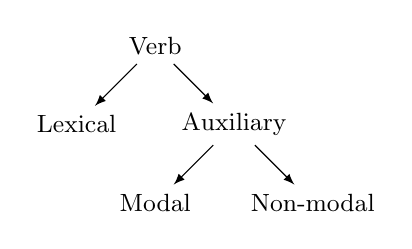
\begin{tikzpicture}[level distance=1cm,
                        sibling distance=2cm,
                        edge from parent/.style={draw, -latex},
                        every node/.style={font=\small, align=center}]

        % Root node
        \node {Verb}
            % First level of branching
            child {node {Lexical}}
            child {node {Auxiliary}
                % Second level of branching
                child {node {Modal}}
                child {node {Non-modal}}
            };

    \end{tikzpicture}
    \caption{Syntactic subclasses of verb}
    \label{fig:verb-structure}
\end{figure}

\noindent When we talk about verbs in English, we're dealing with two main types: lexical verbs and auxiliary verbs. Understanding the difference between them is helpful for grasping how English constructs clauses\is{clause} and conveys certain types of meaning~-- especially since this distinction is far more significant in English than in many other languages\is{cross-linguistic comparison}, such as Spanish\il{Spanish} or Japanese\il{Japanese}, and because auxiliary verbs are involved in a large number of grammatical constructions (e.g., question formation\is{inversion!(subject-auxiliary)} \& negation\is{negation!and auxiliaries|(}).

\textsc{Lexical verbs} make up the vast majority of different English verbs. With a conservative estimate of around 10,000 verbs in English, over 99\% are lexical. These words express actions (\textit{run},\textit{ eat},\textit{ write}), states\is{stative (verb, etc.)} (\textit{exist},\textit{ seem},\textit{ like}), changes (\textit{become},\textit{ grow},\textit{ turn}), and many other situations. In the sentence \textit{The cat sleeps on the couch}, \textit{sleeps} is the lexical verb, even though not much action is going on.

While lexical verbs carry the weight of meaning, \textsc{auxiliary verbs} often bear the burden of grammar. They help form negatives. They help express aspect\is{aspect|(}. They help construct questions and passive voice\is{passive (clause, etc.)!be-passive@\textit{be}-passive}
. No wonder they are often called ``helping verbs''. There are very few, but they are in heavy rotation, making up about 36\% of all verbs in a typical English text.

The auxiliary verbs can be further subdivided into: modal and non-modal auxiliaries. \textsc{Modal auxiliaries} express modality~-- notions like possibility, necessity, or obligation\is{modality!deontic}. The primary modal auxiliaries in English are \textit{will},\textit{ would},\textit{ can},\textit{ could},\textit{ may},\textit{ might},\textit{ shall},\textit{ should}, and \textit{must}. (See Table~\ref{tab:modal-auxiliary-forms} for their tensed forms.) For example, in \textit{I should study more}, \textit{should} is the modal auxiliary expressing obligation, while \textit{study} is the lexical verb.

Each individual modal auxiliary verb typically has a variety of modal meanings: \textit{can}, for instance, is often associated with ability\is{ability (modality)}, but it also expresses other meanings, as shown in (\ref{ex:can-meanings}).

\ea \label{ex:can-meanings}
\ea \textit{She \uline{can} speak three languages.} \hfill(ability)
\ex \textit{You \uline{can} leave early today.} \hfill(permission)
\ex \textit{It \uline{can} be quite cold here in winter.} \hfill(possibility)
\ex \textit{That \uline{can't} be true!} \hfill(logical conclusion)
\z\z

\noindent And though \textit{should} usually expresses obligation, it occasionally substitutes for conditional \textit{if} as in \textit{Should I be late, please go on without me.}

The primary non-modal auxiliaries are \textit{be}, \textit{have}, and \textit{do}.

\begin{itemize}[nosep]
    \item \textit{Be} is used to form the progressive aspect\is{progressive aspect} (\textit{I \uline{am} studying}) and passive voice (\textit{The book \uline{was} written}).
    \item \textit{Have} forms the perfect aspect\is{perfect} (\textit{I \uline{have} studied}).
    \item \textit{Do}\is{do-support@\textit{do}-support|(} is used for emphasis (\textit{I \uline{do} like it}) and in questions (\textit{\uline{Do} you like it?}) and negatives (\textit{No, I \uline{don't} like it}).
\end{itemize}

Few languages rely on auxiliary verbs to the extent that English does. This means that learners from many backgrounds may need extra support to grasp the importance of auxiliaries in forming questions, negatives, and expressing modal meaning in English.

The difference between auxiliaries and lexical verbs becomes clearer when we examine the NICER properties that set auxiliary verbs apart.

\section{The NICER Properties of Auxiliary Verbs}\label{sec:NICER}\is{auxiliary verb!NICER diagnostics|(}

As mentioned in Section \ref{sec:aux}, auxiliary verbs in English have some special properties that set them apart from lexical verbs. These properties are sometimes referred to as the NICER properties, an acronym that stands for Negation\is{negation!and auxiliaries}, Inversion\is{inversion!(subject-auxiliary)}, Contraction\is{contraction}, Ellipsis\is{ellipsis!VP ellipsis}, and Rebuttal. Let's look at each of these in turn.


\begin{table}[ht]
    \centering
    \renewcommand{\arraystretch}{1.5} % Increase general row height
    \begin{tabular}{>{\raggedright\arraybackslash}m{2cm}>{\raggedright\arraybackslash}m{4.5cm}>{\raggedright\arraybackslash}m{4.5cm}}
       
        \textbf{Property} & \textbf{Auxiliary Verb} & \textbf{Lexical Verb} \\
        \textbf{N}egation & \vspace{4pt}\textit{Lee will not eat apples.}\vspace{4pt} & \vspace{4pt}*\textit{Lee eats not apples.}\vspace{4pt} \\
        \textbf{I}nversion & \vspace{4pt}\textit{Has Lee eaten apples?}\vspace{4pt} & \vspace{4pt}*\textit{Eats Lee apples?}\vspace{4pt} \\
        \textbf{C}ontraction & \vspace{4pt}\textit{didn't, shouldn't, isn't}\vspace{4pt} & \vspace{4pt}*\textit{eatn't, gon't, maken't}\vspace{4pt} \\
        \textbf{E}llipsis & \vspace{4pt}\textit{Lee was eating and so was Kim.}\vspace{4pt} & \vspace{4pt}*\textit{Lee kept eating and so kept Kim.}\vspace{4pt} \\
        \textbf{R}ebuttal\is{rebuttal} & 
        \vspace{4pt}\parbox[tl]{4.5cm}{
            A: \textit{We shouldn't eat apples.} \\[0.3cm] 
            B: \textit{We should SO.}
        }\vspace{4pt} & 
        \vspace{4pt}\parbox[tl]{4.5cm}{
            A: \textit{We didn't try to eat apples.} \\[0.3cm] 
            B: *\textit{We tried SO.}
        }\vspace{4pt} \\
    \end{tabular}
    \caption{The NICER properties of auxiliary verbs.}
    \label{tab:nicer-properties}
\end{table}
\is{lexical verb (vs auxiliary)|)}

Negation in English is typically formed by adding \textit{not} after an auxiliary verb. Lexical verbs, on the other hand, require the auxiliary \textit{do} to form negatives\is{negation!with do}. This is called \textsc{do-support@\textit{do}-support}:

\ea
\ea \textit{Lee will not eat apples.}
\ex *\textit{Lee eats not apples.}\footnote{This would have been fine even as recently as Early Modern English\il{English!Early Modern} (the language of Shakespeare\ia{Shakespeare, William}), but not today.}
\ex \textit{Lee does not eat apples.}
\z\z

Inversion describes constructions where the auxiliary verb comes before the subject\is{subject!and auxiliaries}, such as certain types of questions\is{clause type!and inversion}. Again, lexical verbs need \textit{do} for this:

\protectedex{
\ea
\ea \textit{Has Lee eaten apples?}
\ex *\textit{Eats Lee apples?}
\ex \textit{Does Lee eat apples?}
\z\z}

Inversion for question formation is not a feature shared by a wide range of languages. English learners commonly omit \textit{do} in negation and inversion, likely because it contributes only syntactically, not semantically. For example, they might say \textit{I not like apples} or \textit{He eat apples?} without \textit{do}-support.

``Contraction'' allows \textit{not} to be shortened to \textit{n't} and suffixed to most auxiliary verbs. This isn't possible with lexical verbs:

\ea \textit{didn't}, \textit{shouldn't}, \textit{isn't}
\ex *\textit{eatn't}, *\textit{gon't}, *\textit{maken't}
\z

Ellipsis permits a verb phrase to be understood from the context instead of appearing overtly:

\ea \textit{Lee was eating apples, and Kim was {\op}eating them{\cp} too.}
\ex *\textit{Lee kept eating apples, and Kim kept {\op}eating them{\cp} too.}
\z

Rebuttal\is{rebuttal} uses auxiliary verbs along with \textit{so}, \textit{too}, or \textit{indeed}, to contradict a previous negative statement:

\ea A: \textit{We shouldn't eat apples.}\\
B: \textit{We should SO.}
\ex A: \textit{We didn't try to eat apples.}
\\ B: *\textit{We tried SO.}
\z

The NICER properties are not just helpful diagnostics, they actually identify many of the things about auxiliary verbs that make them challenging for our students. For example, it explains why we say \textit{Don't you like it?} instead of *\textit{You no like it?}, or why you might utter the assertion \textit{I do like it}.\is{negation!and auxiliaries|)}\is{do-support@\textit{do}-support|)}

In the next section, we'll look at the various forms that verbs can take in English, which will set us up to discuss tense and aspect.

\begin{tcolorbox}[title=Exercise: Basic Verb Types, colback=white, colframe=blue!75!black, fonttitle=\bfseries]
Identify whether the underlined verbs in the following sentences are lexical or auxiliary. If auxiliary, specify whether they are modal or non-modal. Remember that some auxiliary verbs have a matching lexical verb.

\begin{enumerate}[nosep]
    \item \textit{The cat \uline{sleeps} on the couch.}
    \item \textit{I \uline{will} attend the meeting tomorrow.}
    \item \textit{She \uline{has} a test tomorrow.}
    \item \textit{She \uline{has} finished her homework.}
    \item \textit{\uline{Did} she \uline{do} her homework?}
    \item \textit{They \uline{are} planning a surprise party.}
    \item \textit{It'\uline{s} at my house.}
    \item \textit{It \uline{is} not.}
    \item \textit{You \uline{must} complete the assignment by Friday.}
    \item \textit{I don't think I \uline{can}.}
\end{enumerate}
For each of the following sentences, apply one of the NICER properties (Negation, Inversion, Contraction, Ellipsis, or Rebuttal) to create a new, grammatically correct sentence. Identify which property you used.

\begin{enumerate}[nosep]
    \item \textit{She can swim very well.}
    \item \textit{They have finished the project.}
    \item \textit{We are having lunch.}
    \item \textit{You should try it.}
    \item \textit{Do you study grammar?}
\end{enumerate}

Example: \textit{He's Cambodian.} $\rightarrow$ \textit{He isn't Cambodian.} (Contraction)
\end{tcolorbox}
\is{NICER properties|)}\is{auxiliary verb!NICER diagnostics|)}

\section{Verb Forms}\label{sec:verb-forms}

English verbs, whether lexical or auxiliary, have several different forms. As a proficient English speaker, you already know their syntax, morphology, and spelling, but, as an English teacher, being able to identify them is useful for understanding and explaining clause structure and the English tense and aspect system.

The \textsc{plain form}\is{plain form of verb} is the simplest form of the verb. It's the ``dictionary form''.

\ea \textit{arrive}, \textit{be}, \textit{come}, \textit{do}, \textit{eat}, \textit{fall}, \textit{go}, \textit{have}, \textit{interrupt}
\z

\begin{table}[ht]
    \centering
    \begin{tabular}{ccccccc}
       
        \textbf{Plain} & \multicolumn{3}{c}{\textbf{Tensed}} & \multicolumn{2}{c}{\textbf{Participles}} \\
        & \multicolumn{2}{c}{\textbf{Present}} & \textbf{Past} & \textbf{Present} & \textbf{Past} \\
        & plain & 3rd pers sing & &  &  \\
        \textit{jump} & \textit{jump} & \textit{jumps} & \textit{jumped} & \textit{jumping} & \textit{jumped} \\
        \textit{go} & \textit{go} & \textit{goes} & \textit{went} & \textit{going} & \textit{gone} \\
        \textit{eat} & \textit{eat} & \textit{eats} & \textit{ate} & \textit{eating} & \textit{eaten} \\
        \textit{put} & \textit{put} & \textit{puts} & \textit{put} & \textit{putting} & \textit{put} \\
        \textit{keep} & \textit{keep} & \textit{keeps} & \textit{kept} & \textit{keeping} & \textit{kept} \\
    \end{tabular}
    \caption{Verb Forms: Plain, Tensed, and Participles}
    \label{tab:verb-forms}
\end{table}

The \textsc{plain present form}\is{present tense/non-past} is identical to the plain form for all verbs (see Table \ref{tab:verb-forms}) except \textit{be}, which has an unusual number of present forms: \textit{am}, \textit{is}, and \textit{are}.

\ea \textit{arrive}, \textit{come}, \textit{do}, \textit{eat}, \textit{fall}, \textit{go}, \textit{have}, \textit{interrupt}
\z
The \textit{-s} form\is{s form@-\textit{s} verb form}, or the \textsc{third-person singular present form}\is{third-person singular present form}, adds \textit{-{\op}e{\cp}s} to the plain form, with a few irregular forms, as in (\ref{ex:3sing-pres}).

\ea \textit{arrives}, \textit{is}, \textit{comes}, \textit{does}, \textit{eats}, \textit{falls}, \textit{goes}, \textit{has}, \textit{interrupts}\label{ex:3sing-pres}
\z
The \textsc{past form}\is{past tense} is used for the simple past tense. Regular verbs add \textit{-ed}, but many common verbs have irregular past forms:

\ea \textit{arrived}, \textit{was}/\textit{were}, \textit{came}, \textit{did}, \textit{ate}, \textit{fell}, \textit{went}, \textit{had}, \textit{interrupted}\label{ex:past-tense-forms}
\z
The \textit{-ing} form\is{ing form@-\textit{ing} verb form}, also known as the \textsc{present participle}\is{present participle}\label{sec:participles},\footnote{CGEL uses the term \textsc{gerund-participle}\is{gerund-participial (verb-form)} for this form.} is used to form the progressive aspect, among other things:

\ea \textit{arriving}, \textit{being}, \textit{coming}, \textit{doing}, \textit{eating}, \textit{falling}, \textit{going}, \textit{having}, \textit{interrupting}\label{ex:-ing}
\z

\begin{tcolorbox}[title=What about gerunds?\is{gerund}, colback=white]

You may have heard about \textsc{gerunds}~-- verbs in the \textit{-ing} form that ``function as nouns''~-- as in the underlined phrases in (\ref{ex:merely-looking} \& \ref{ex:making-dinner}).

\ea\textit{\uline{Merely looking} can make a difference.}\label{ex:merely-looking}
\ex\textit{I actually enjoy \uline{making dinner} after a long day,} \label{ex:making-dinner}
\z

~~~~The problem is that the idea of a verb functioning as a noun is as odd that of a goldfish functioning as a dog; while both species may function as pets, their fundamental natures remain distinct. Similarly, \textsc{subject}\is{subject} and \textsc{complement}\is{complement, complementation!in clause/VP} are functions, but \textsc{noun} is what a word intrinsically is. So, are \textit{looking} and \textit{making} fundamentally nouns or verbs?

~~~~In considering this question, you should return to the characteristics of nouns and verbs you encountered in Sections \ref{sec:nouns} and \ref{sec:verbs}. If the underlined phrases in (\ref{ex:merely-looking} \& \ref{ex:making-dinner}) were NPs, then we might expect them to allow plural forms and AdjP modifiers. They don't. Instead, they allow AdvP\is{adverb, adverb phrase (AdvP)} modifiers\is{modifier/modification} as in \textit{merely looking} and license objects\is{object!direct} as in \textit{making dinner}. These are the characteristics of VPs.

~~~~That's not to say that there aren't \textit{-ing} nouns, but they're not so common. They show up in examples like  (\ref{ex:the-opening} \& \ref{ex:building-of}).

\ea    \textit{The \uline{opening} of the new store attracted a large crowd.} \label{ex:the-opening}
\ex   \textit{The city funded the \uline{building} of the bridge.}\label{ex:building-of}
\z

In such cases, the \textit{-ing} words are true nouns:

\begin{itemize}[nosep]
    \item They can be pluralized: \\\textit{The \uline{openings} of the new stores were scheduled for next month.}
    \item They can be modified by adjectives: \\\textit{The \uline{grand opening} of the new store was a success.}
    \item They require a prepositional phrase with \textit{of} to introduce their complement: \textit{The building \uline{of} the bridge}, not *\textit{The building the bridge}.
\end{itemize}

These characteristics align with what we expect of nouns.

~~~~So what to do with the term ``gerund''. Personally, I don't find it useful for discussing the English of today. Instead, I would simply say that the subject of  (\ref{ex:merely-looking}) is a VP, as is the complement of \textit{enjoy} in (\ref{ex:making-dinner}).\footnote{\textit{CGEL} would call these clauses, not VPs.}

\end{tcolorbox}

The \textsc{past participle}\is{past participle} has various grammatical roles, including forming the perfect aspect and passive constructions. For regular verbs, it's identical to the past form (sometimes called the preterite), but many irregular verbs have distinct past participles:

\ea \textit{arrived}, \textit{been}, \textit{come}, \textit{done}, \textit{eaten}, \textit{fallen}, \textit{gone}, \textit{had}, \textit{interrupted}\label{ex:past-participles}
\z

Most lexical verbs\is{lexical verb (vs auxiliary)} have all six of these forms, but modal auxiliaries are \textsc{defective}\is{defective verbs}\is{modal auxiliaries!defectiveness}~-- they lack the plain form and participles.\label{sec:defective-modals}

\ea \textit{can}/\textit{could}, \textit{will}/\textit{would}, \textit{shall}/\textit{should}, \textit{may}/\textit{might}, \textit{must}/--
\z

\noindent The auxiliary verbs, modal or not, also have negative and contracted forms.\is{tense|(}

\begin{table}[ht]
    \centering
    \begin{tabular}{cccccc}
       
        \multicolumn{3}{c}{\textbf{Present Tense}} & \multicolumn{3}{c}{\textbf{Past Tense}} \\
         & Contracted & Negative &  & Contr. & Negative \\
        \textit{will} & \textit{'ll} & \textit{won't} & \textit{would} & \textit{'d} & \textit{wouldn't} \\ 
        \textit{may} & & & \textit{might} & & \textit{mightn't} \\ 
        \textit{can} & & \textit{can't}, \textit{cannot} & \textit{could} & & \textit{couldn't} \\ 
        \textit{shall} & \textit{'ll} & \textit{shan't} & \textit{should} & & \textit{shouldn't} \\ 
        \textit{must} & & \textit{mustn't} & & & \\
        \textit{do} & \textit{do}(\textit{es})\textit{n't} & & \textit{did} & \textit{didn't} & \\ 
        \textit{have} & \textit{'ve}/\textit{'s} & \textit{haven't}/\textit{hasn't} & \textit{had} & \textit{'d} & \textit{hadn't} \\ 
        \textit{be} & \textit{'m}/\textit{'re}/\textit{'s} & \textit{--}/\textit{aren't}/\textit{isn't} & \textit{was}/\textit{were} & & \textit{wasn't}/\textit{weren't} \\
    \end{tabular}
    \caption{Tensed auxiliary verb forms}
    \label{tab:modal-auxiliary-forms}
\end{table}
\is{modal auxiliary|)}

\noindent The non-modal auxiliaries~-- \textit{do}, \textit{have}, and \textit{be}~-- also have plain, present-participle, and past participle forms. It's also worth noting that these three verbs also have lexical-verb counterparts. In each case, we know they're not modal because the NICER properties don't apply.

\ea
\ea \textit{Don't \uline{be} late.}\label{ex:lexical-be}
\ex \textit{I \uline{have} a cat.}\label{ex:lexical-have}
\ex \textit{I \uline{do} my homework every day.}\label{ex:lexical-do}
\z\z
In (\ref{ex:lexical-be}), we can't have *\textit{Be not late} or even *\textit{ben't}. In (\ref{ex:lexical-have}), we have the verb of belonging, not the one that forms the perfect aspect. We don't ask \textit{Have you a cat?} or say \textit{I haven't a cat} (at least not in most present-day North American dialects). And if we want to ask about doing your homework, we need an auxiliary \textit{do} (underlined) to go with the lexical \textit{do}: \textit{\uline{Do} you do your homework?}

The verb \textit{be} is highly irregular, with more forms than any other English verb:

\ea
\ea \textit{be}, \textit{am}, \textit{is}, \textit{are}, \textit{was}, \textit{were}, \textit{being}, \textit{been}
\ex \textit{isn't}, \textit{aren't}, \textit{wasn't}, \textit{weren't}
\ex \textit{'m}, \textit{'s}, \textit{'re}
\z\z

The various verb forms combine with auxiliaries to create the tense and aspect system. For instance, the present perfect\is{present perfect} uses \textit{have} + the past-participle form:\footnote{In \cite{Huddleston2002}\ia{Huddleston, Rodney}\ia{Pullum, Geoffrey K.}, the perfect is a secondary past tense, but I don't find that analysis helpful here, and so I don't follow it.}

\ea \textit{I have eaten.}
\ex \textit{She has gone.}
\z

The past progressive combines the past of \textit{be} with the \textit{-ing} form:

\ea \textit{I was reading.}
\ex \textit{They were sleeping.}
\z\is{progressive aspect}\is{perfect}

\begin{tcolorbox}[title=Exercise: Verb Forms, colback=white, colframe=red!75!black, fonttitle=\bfseries]
Identify the verb form (1. plain, 2. plain present, 3. third-person singular present, 4. past, 5. present participle, or 6. past participle) for each underlined verb.

\begin{enumerate}[nosep]
    \item \textit{She \uline{sings} beautifully.} \hfill\uline{~~~~}
    \item \textit{They \uline{may} \uline{have} \uline{gone} to the store.} \hfill\uline{~~~~},  \uline{~~~~},  \uline{~~~~}
    \item \textit{We \uline{were} \uline{watching} a movie.} \hfill\uline{~~~~},  \uline{~~~~}
    \item \textit{The dog \uline{barked} all night.} \hfill\uline{~~~~}
    \item \textit{I \uline{write} in my journal every day.} \hfill\uline{~~~~}
    \item \textit{I'\uline{ll} \uline{try} again.} \hfill\uline{~~~~},  \uline{~~~~}
\end{enumerate}
\end{tcolorbox}
\is{auxiliary verb|)}\is{complement, complementation|)}\is{tense|)}\is{aspect|)}

\section{Aspect}\is{aspect|(}
If tense is primarily about when something happens, \textsc{aspect} is more about the temporal perspective we take on a situation. But what does that really mean?

\subsection{The progressive aspect}\is{progressive aspect|(}\label{sec:progressive-aspect}
Let's start with a seemingly simple question: what's the difference between these two sentences?

\ea
\ea \textit{I live in Mississauga.} \hfill(simple aspect) \label{ex:I-live}
\ex \textit{I'm living in Mississauga.} \hfill(progressive aspect) \label{ex:Im-living}
\z\z

At first glance, these sentences might appear identical~-- both state my city of residence and both are factually correct. But there's a subtle distinction: (\ref{ex:I-live}) suggests an indifference to the duration of the situation, while (\ref{ex:Im-living}) asserts the relevance of its temporariness. This difference in perspective is illustrated in Figure~\ref{fig:enter-label}.

\begin{figure}[ht]
    \centering
    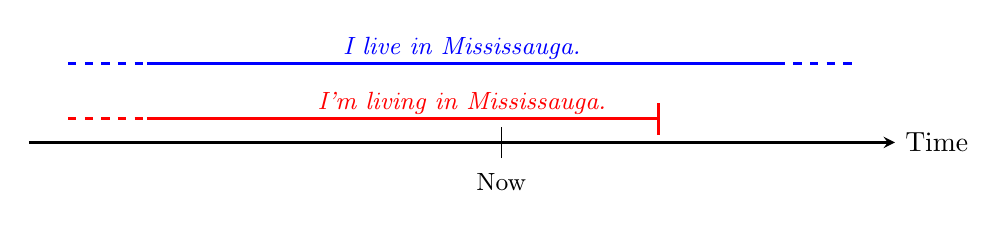
\begin{tikzpicture}[scale=1]
        % Define styles
        \tikzset{
            timeline/.style={->, >=stealth, thick},
            label/.style={font=\small}
        }
        % Draw the main timeline
        \draw[timeline] (-1,0) -- (10,0) node[right] {Time};
        % "Now" point on timeline
        \draw (5,-0.2) -- (5,0.2);
        \node[label] at (5,-0.5) {Now};
        % "I live in Mississauga" (Simple aspect)
        \draw[blue, very thick, dashed] (-0.5,1) -- (0.5,1);
        \draw[blue, very thick] (0.5,1) -- (8.5,1);
        \draw[blue, very thick, dashed] (8.5,1) -- (9.5,1);
        \node[label, blue] at (4.5,1.2) {\textit{I live in Mississauga.}};
        % "I'm living in Mississauga" (Progressive aspect)
        \draw[red, very thick, dashed] (-0.5,0.3) -- (0.5,0.3);
        \draw[red, very thick] (0.5,0.3) -- (7,0.3);
        \node[label, red] at (4.5,0.5) {\textit{I'm living in Mississauga.}};
        \draw[red, very thick] (7,0.5) -- (7,0.1);  % End vertical bar
    \end{tikzpicture}
    \caption{Comparison of the simple and progressive aspects for \textit{I live in Mississauga} on a timeline.}
    \label{fig:enter-label}
\end{figure}

Anyone might say (\ref{ex:I-live}) in the simple aspect, but only someone like an international student attending University of Toronto would choose the progressive aspect of (\ref{ex:Im-living}). While all situations are ultimately ephemeral, the progressive aspect, formed with $be+-ing$ expresses relevance not just to what continues but to its conclusion. The simple aspect, in contrast, draws no special attention to endings.

To illustrate this shift in viewpoint, consider the difference between paddling a river that flows into the sea vs paddling one that comes to a dam. It's the same body of water either way, but in the first, you're aware only of the water, while in the second, the dam requires your attention.

Unlike these paddlers, a speaker typically has a choice of how to portray the situation. The selection of one aspect or the other invites the audience to consider the situation from a particular vantage point, with neither being grammatically better.

\subsubsection{States often resist the progressive aspect}\label{sec:statives-resist}
Sometimes, though, one perspective really does seem wrong to certain groups of speakers. Consider, for instance, (\ref{ex:know-knowing}).

\ea \label{ex:know-knowing}
\ea \textit{I know that feeling.}
\ex *\textit{I'm knowing that feeling.}
\z\z

The progressive in (\ref{ex:know-knowing}b) implies that an endpoint to this knowledge is relevant, a perspective that feels unnatural. For many speakers of English, drawing attention to the potential cessation of knowing is odd, not because knowledge can't end~-- people do forget~-- but because it's so clearly not relevant. The simple aspect, by contrast, allows us to focus on the current state of knowing without unnecessary implications about its duration.\footnote{\ref{ex:know-knowing}b is, nevertheless, quite common in South Asian English\il{English!South Asian}, for example.}

The same applies to other verbs. Consider the stative\is{stative (verb, etc.)|(} examples in (\ref{ex:stative-verbs}). The (a) sentences with the simple aspect are fine, but the (b) examples in the progressive are ungrammatical.

\ea\label{ex:stative-verbs}
\ea \textnormal{i.} \textit{Birds have feathers.} \\ \textnormal{ii.} \textit{Earth is a planet.} \\ \textnormal{iii.} \textit{Honey tastes sweet.}
\ex \textnormal{i.} *\textit{Birds are having feathers.} \\ \textnormal{ii.} *\textit{Earth is being a planet.} \\ \textnormal{iii.} *\textit{Honey's tasting sweet.}
\z\z

The end of birds having feathers, of Earth being a planet, or of honey tasting sweet might be relevant in some peculiar context, but it's scarcely conceivable what that context might be. By asking us to take an irrelevant perspective with these \textsc{stative verbs}, the progressive aspect creates a linguistic mismatch and registers as ungrammatical.

And yet, sometimes it works, as in (\ref{ex:prog-statives}).

\ea\label{ex:prog-statives}
\ea \textit{We're having dinner.}
\ex \textit{He's being grumpy.}
\ex \textit{It's tasting sweeter.}
\z\z

In these cases, the progressive aspect fits because the impending end of the state matters. I can call you back when the meal is over, it would be better to talk to him when he's no longer grumpy, and presumably, the honey will soon return to its usual taste once the effect of whatever changed it has worn off. These examples demonstrate that the progressive aspect isn't inherently ungrammatical with stative verbs. It's just not usually a good fit.\is{stative (verb, etc.)|)}

\subsubsection{Progressive aspect for limited repetition}\is{progressive aspect|(}
While most actions take time, others are instantaneous: \textit{the light flashed, she sneezed, it popped, he blinked, the show ended}. In cases like these, the progressive aspect can still be used. But rather than inviting us to consider the end of a single situation, it asserts the relevance of the end of a series of events. \textit{I'm falling} may be a long drawn out descent, but \textit{She's sneezing} doesn't imply a super slow-mo spit-spraying expulsion of air. Instead it presents a set of sternutations for which an end is in sight.

This interpretation of the progressive aspect as indicating a limited series isn't restricted to momentary events. \textit{I'm going to the gym regularly} is the claim of a person who's not sure how long they can keep up the commitment or has a limited-term membership, as in Figure~\ref{fig:regular-gym-visits}.

\begin{figure}[ht]
    \centering
    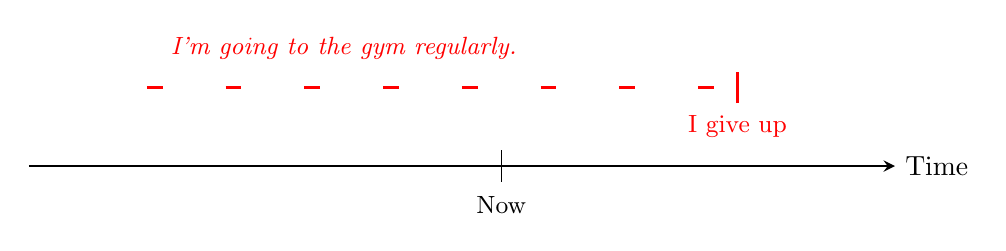
\begin{tikzpicture}[scale=1]
        % Define styles
        \tikzset{
            timeline/.style={->, >=stealth, thick},
            label/.style={font=\small}
        }
        % Draw the main timeline
        \draw[timeline] (-1,0) -- (10,0) node[right] {Time};
        % "Now" point on timeline
        \draw (5,-0.2) -- (5,0.2);
        \node[label] at (5,-0.5) {Now};
        % "end" point on timeline
        \draw[red, very thick] (8,0.8) -- (8,1.2);
        \node[label, red] at (8,0.5) {I give up};
        % Event instances (e.g., gym visits)
        \foreach \x in {0.5, 1.5, 2.5, 3.5, 4.5, 5.5, 6.5, 7.5}
            \draw[red, very thick] (\x,1) -- (\x+0.2,1);
        % Labels for periodic gym visits
        \node[label, red] at (3, 1.5) {\textit{I'm going to the gym regularly.}};
    \end{tikzpicture}
    \caption{Timeline for the progressive aspect in \textit{I'm going to the gym regularly}.}
    \label{fig:regular-gym-visits}
\end{figure}

Another illustrative example of this phenomenon is \textit{I'm eating at that new restaurant}. While eating a meal is not an instantaneous action, the use of the progressive aspect here doesn't necessarily imply that the speaker is currently in the middle of a meal at the restaurant. Instead, it suggests a series of visits until something new comes along.

In the gym example, the use of \textit{regularly} makes the repeated-temporary-action interpretation the only possible meaning of the progressive. The restaurant example, though, is ambiguous. If said outside the restaurant, then it implies serial patronage. If inside, perhaps it refers to a meal that will end before some other relevant event.

\subsubsection{The progressive for plans}
The progressive aspect has yet more uses. It can also express future plans, as it does in (\ref{ex:dinner-next-week}).

\ea \textit{The Smiths are having dinner with us this week.}\label{ex:dinner-next-week}
\z

This doesn't imply an ongoing, extended feast. Rather, it encapsulates the planning and anticipation of the event. This usage presupposes that the dinner has been arranged; the progressive aspect wouldn't be appropriate if the idea had just occurred and the Smiths hadn't been invited yet. The progressive here spans from the moment of agreement (the start) to the anticipated conclusion of the dinner (the end).
\is{progressive aspect|)}

\begin{figure}[ht]
    \centering
    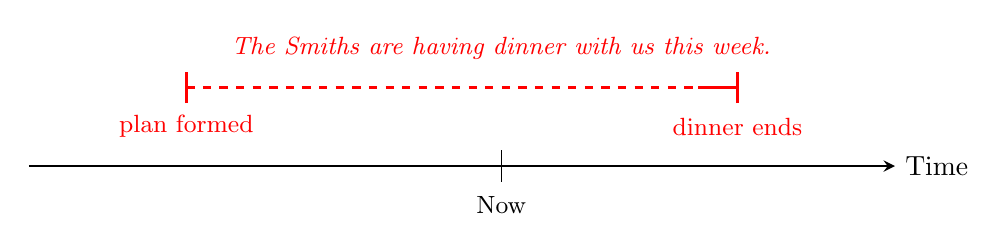
\begin{tikzpicture}[scale=1]
        % Define styles
        \tikzset{
            timeline/.style={->, >=stealth, thick},
            label/.style={font=\small}
        }
        % Draw the main timeline
        \draw[timeline] (-1,0) -- (10,0) node[right] {Time};
        % "Now" point on timeline
        \draw (5,-0.2) -- (5,0.2);
        \node[label] at (5,-0.5) {Now};
        % "We're having dinner with the Smiths next week" (Future Progressive aspect)
        \draw[red, very thick, dashed] (1,1) -- (7.5,1); % Planning phase - from now
        \draw[red, very thick] (7.5,1) -- (8,1); % Future event
        \draw[red, very thick] (1,0.8) -- (1,1.2); % Start boundary of event
        \draw[red, very thick] (8,0.8) -- (8,1.2); % End boundary of event
        \node[label, red] at (5,1.5) {\textit{The Smiths are having dinner with us this week.}};
        % Add "planned" below the planning phase
        \node[label, red] at (1, 0.5) {plan formed};
        % Add "dinner" below the planning phase
        \node[label, red] at (8, 0.5) {dinner ends};
    \end{tikzpicture}
    \caption{Representation of the ``planned future'' use of the progressive aspect for \textit{We're having dinner with the Smiths next week.}}
    \label{fig:futurate-progressive}
\end{figure}
\is{progressive aspect|)}

\subsection{The perfect aspect}\is{perfect|(}\label{sec:perfect-aspect}
While the progressive aspect focuses on the ongoing nature of a situation, English has another aspect that expresses a different temporal perspective: the perfect. The perfect aspect, formed with a form of have + past participle\is{past participle|(}, asserts the relevance of a previous situation (or action, etc) to a later time.

The reference time can be in the present, past, or even in the future, but let's start with the present perfect\is{present perfect|(}. This uses the present tense and has "now" as a reference time. Consider (\ref{ex:have-lived}).

\ea \textit{I've lived in Mississauga for five years.}\label{ex:have-lived}
\z

In its most salient sense, this sentence conveys a situation that began in the past and continues to be true in the present. It stretches back for five years and remains relevant now. To appreciate the nuance of the perfect aspect, let's compare it to the simple past\is{past tense}:

\ea \textit{I lived in Mississauga for five years.}\label{ex:lived}
\z

In (\ref{ex:lived}), I'm talking about a situation fully in the past. I no longer live there. The cases of the present-perfect (\ref{ex:have-lived}) case and the simple past (\ref{ex:lived}) are contrasted in Figure~\ref{fig:past-vs-present-perfect}. Non "now" reference times are shown in Figures~\ref{fig:past-perfect}--\ref{fig:timeless-perfect}. In each case, the perfect aspect connects two time points: the time of the situation itself and the subsequent reference time to which it's relevant. This allows speakers to express complex temporal relationships and emphasize the significance of past (or completed future) situations to other points in time.

\begin{figure}[ht]
    \centering
    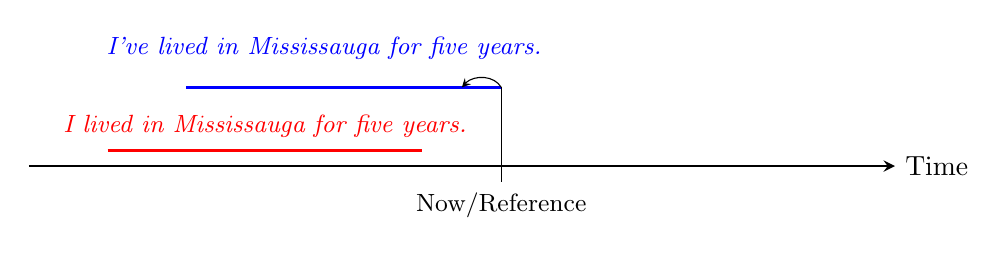
\begin{tikzpicture}[scale=1]
        % Define styles
        \tikzset{
            timeline/.style={->, >=stealth, thick},
            label/.style={font=\small}
        }
        % Draw the main timeline
        \draw[timeline] (-1,0) -- (10,0) node[right] {Time};
        % "Now" point on timeline
        \draw (5,-0.2) -- (5,1);
        \node[label] at (5,-0.5) {Now/Reference};
        % "I've lived in Mississauga for five years" (Present Perfect aspect)
        \draw[blue, very thick] (1,1) -- (5,1); % From past to now
        \node[label, blue] at (2.75,1.5) {\textit{I've lived in Mississauga for five years.}};
        % "I lived in Mississauga for five years" (Simple Past aspect)
        \draw[red, very thick] (0,0.2) -- (4,0.2); % A completed action in the past, same length but before now
        \node[label, red] at (2,0.5) {\textit{I lived in Mississauga for five years.}};
        % Arcing arrow
        \draw[->, >=stealth, bend right=60] (5,1) to (4.5,1);
    \end{tikzpicture}
    \caption{Comparison of the present perfect and simple past for \textit{I lived in Mississauga for five years.} The reference point is ``now''.}
    \label{fig:past-vs-present-perfect}
\end{figure}

\begin{figure}[ht]
    \centering
    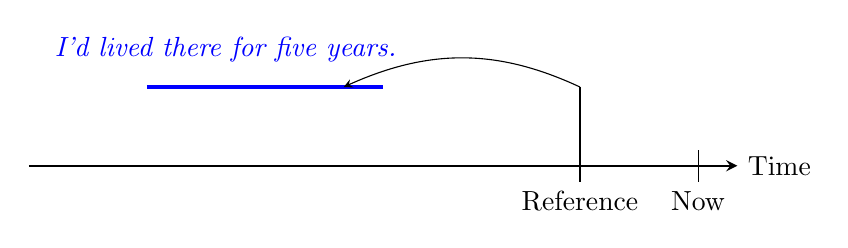
\begin{tikzpicture}
        % Timeline
        \draw[->, >=stealth, thick] (0,0) -- (9,0) node[right] {Time};
        % "Reference" point
        \draw (7,-0.2) -- (7,1);
        \node[below] at (7,-0.2) {Reference};
        % "Now" point
        \draw (8.5,-0.2) -- (8.5,0.2);
        \node[below] at (8.5,-0.2) {Now};
        % Past perfect duration
        \draw[blue, very thick] (1.5,1) -- (4.5,1);
        % Example text
        \node[blue, above] at (2.5,1.2) {\textit{I'd lived there for five years.}};
        % Arcing arrow
        \draw[->, >=stealth, bend right=25] (7,1) to (4,1);
    \end{tikzpicture}
    \caption{Representation of the past perfect: \textit{I'd lived there for five years.} The reference point is before ``now'', and the situation is fully before that point.}
    \label{fig:past-perfect}\is{past perfect}
\end{figure}

\begin{figure}[ht]
    \centering
    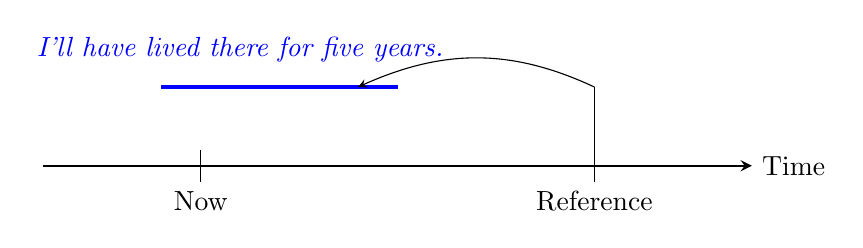
\begin{tikzpicture}
        % Timeline
        \draw[->, >=stealth, thick] (0,0) -- (9,0) node[right] {Time};
        % "Now" point
        \draw (2,-0.2) -- (2,0.2);
        \node[below] at (2,-0.2) {Now};
        % "reference" point
        \draw (7,-0.2) -- (7,1);
        \node[below] at (7,-0.2) {Reference};
        % Futurate perfect duration
        \draw[blue, very thick] (1.5,1) -- (4.5,1);
        % Example text
        \node[blue, above] at (2.5,1.2) {\textit{I'll have lived there for five years.}};
        % Arcing arrow
        \draw[->, >=stealth, bend right=25] (7,1) to (4,1);
    \end{tikzpicture}
    \caption{Representation of the futurate perfect: \textit{I'll have lived there for five years.} The reference point after ``now'' and the event is before that point. Note the ``now'' could be anywhere before the end of the blue line.}
    \label{fig:futurate-perfect}\is{futurate}
\end{figure}

\begin{figure}[ht]
    \centering
    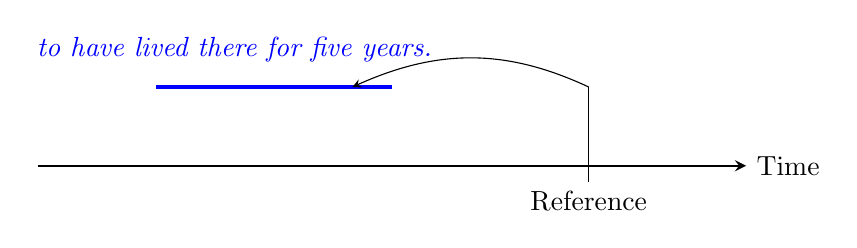
\begin{tikzpicture}
        % Timeline
        \draw[->, >=stealth, thick] (0,0) -- (9,0) node[right] {Time};
        % "reference" point
        \draw (7,-0.2) -- (7,1);
        \node[below] at (7,-0.2) {Reference};
        % Futurate perfect duration
        \draw[blue, very thick] (1.5,1) -- (4.5,1);
        % Example text
        \node[blue, above] at (2.5,1.2) {\textit{to have lived there for five years.}};
        % Arcing arrow
        \draw[->, >=stealth, bend right=25] (7,1) to (4,1);
    \end{tikzpicture}
    \caption{Representation of the timeless perfect: \textit{To have lived there for five years is quite an experience.} The reference point is any time.}
    \label{fig:timeless-perfect}
\end{figure}

The perfect aspect can sometimes lead to ambiguity. The situation must begin prior to the reference time, but whether or not it is complete at the reference time is open to interpretation. As a result, the red line in Figure~\ref{fig:present-perfect-simple-past} representing the simple past and the blue line immediately above it may refer to exactly the same period of time, just from different perspectives. The ambiguity can usually be resolved from the context, or from some modifier such as \textit{already} (completed).

\begin{figure}[ht]
    \centering
    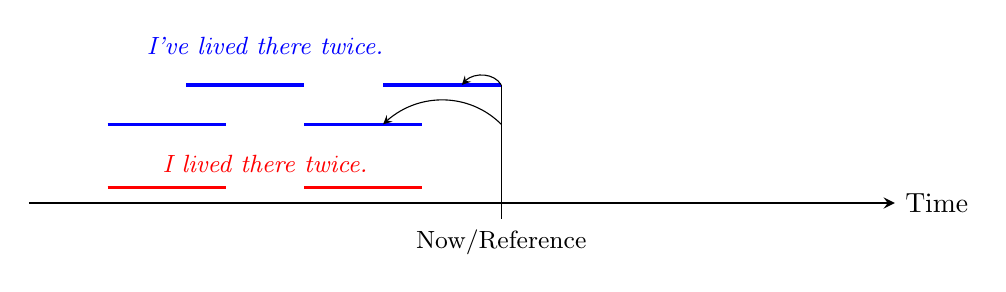
\begin{tikzpicture}[scale=1]
        % Define styles
        \tikzset{
            timeline/.style={->, >=stealth, thick},
            label/.style={font=\small}
        }
        % Draw the main timeline
        \draw[timeline] (-1,0) -- (10,0) node[right] {Time};
        % "Now" point on timeline
        \draw (5,-0.2) -- (5,1.5);
        \node[label] at (5,-0.5) {Now/Reference};
        % "I've lived in Mississauga for five years" (Present Perfect aspect)
        \draw[blue, very thick] (0,1) -- (1.5,1);
        \draw[blue, very thick] (2.5,1) -- (4,1); % From past to now
        % "I've lived in Mississauga for five years" (Present Perfect aspect)
        \draw[blue, very thick] (1,1.5) -- (2.5,1.5);
        \draw[blue, very thick] (3.5,1.5) -- (5,1.5); % From past to now
        \node[label, blue] at (2,2) {\textit{I've lived there twice.}};
        % "I lived in Mississauga for five years" (Simple Past aspect)
        \draw[red, very thick] (0,0.2) -- (1.5,0.2);
        \draw[red, very thick] (2.5,0.2) -- (4,0.2); % A completed action in the past, same length but before now
        \node[label, red] at (2,0.5) {\textit{I lived there twice.}};
        % Arcing arrow
        \draw[->, >=stealth, bend right=45] (5,1) to (3.5,1);
        % Arcing arrow
        \draw[->, >=stealth, bend right=60] (5,1.5) to (4.5,1.5);
    \end{tikzpicture}
    \caption{Comparison of the present perfect and simple past for two periods of residence. The reference point is ``now''.}
    \label{fig:present-perfect-simple-past}
\end{figure}

As you explain these distinctions to your students, you might find yourself grappling with questions like: Why does English need all these different ways of talking about time? How do other languages express these nuances? And how can we help our students not just understand these forms, but feel them intuitively?\is{present perfect|)}\is{perfect|)}

\begin{tcolorbox}[title=Exercise: Aspect, colback=white, colframe=purple!75!black, fonttitle=\bfseries]
Identify the aspect (simple, progressive, or perfect) in each sentence and explain the temporal perspective it conveys.

\begin{enumerate}[nosep]
    \item \textit{I've worked here for ten years.} \hfill\uline{\hspace{2cm}} tense
    \item \textit{She was reading when the phone rang.} \hfill\uline{\hspace{2cm}} tense~~\uline{\hspace{2cm}} tense
    \item \textit{We play tennis every Saturday.} \hfill\uline{\hspace{2cm}} tense
    \item \textit{They will have completed the course by June.} \hfill\uline{\hspace{2cm}} tense~~\uline{\hspace{2cm}} tense
    \item \textit{The sun is setting earlier these days.}  ~\hfill\uline{\hspace{2cm}} tense
\end{enumerate}
\end{tcolorbox}
\is{past participle|)}
\is{aspect|)}

\section{Tense Across Languages}\is{cross-linguistic comparison|(}

Imagine for a moment that you're learning a language where verbs don't change to show when something happened. No \textit{-ed} endings for past tense, no \textit{will}. How would you talk about time? It might seem impossible, but for speakers of many languages, this is perfectly normal.

In Mandarin Chinese\il{Chinese, Mandarin}, for instance, the verb form stays the same regardless of when the action occurs:

\ea \textit{Wǒ chī píngguǒ.} (I eat apple)\label{ex:chī}
\z
Example (\ref{ex:chī}) could mean `I eat apples', `I ate an apple', `I'm eating an apple', or `I will eat an apple', depending on the context. Time is often indicated by other words like the equivalent of \textit{tomorrow} or \textit{before}, or it's left to context.

As English speakers, we might find this mind-boggling. But before we get too comfortable with our own tense system, consider the Yimas\il{Yimas} language of Papua New Guinea. It has not two, not three, but seven distinct tenses:\footnote{Some Yimas forms encode both tense and aspect, making them better analyzed as tense--aspect amalgams rather than pure tenses.}

\ea
\ea \textit{wa-ntut} \hfill`went more than a few days ago'
\ex \textit{wa-kiantut} \hfill`went a few days ago'
\ex \textit{wa-nan} \hfill`went yesterday'
\ex \textit{wa-t} \hfill`went today'
\ex \textit{wa-n} \hfill`going now'
\ex \textit{wa-wat} \hfill`usually go'
\ex \textit{wa-kiak} \hfill`will go tomorrow'
\ex \textit{wa-kt} \hfill`will go after tomorrow'
\z\z

These examples highlight a crucial point: the way we conceptualize and express time is not universal. It's just the way each speech community has come to, and speakers of other languages have often arrived at different conventions.

So, given this diversity, how many tenses would you guess English has? Three? Sixteen? In fact, English has \dots

\begin{tcolorbox}[title=Exercise: Comparing Tense and Aspect Across Languages, colback=white, colframe=blue!75!black, fonttitle=\bfseries]

Often the elements that seem very important in one language are simply left out in another. English speakers learning French\il{French} often want to translate the progressive aspect directly, and French has a form for that: \textit{I'm doing it} can be translated as \textit{Je suis en train de le faire.} But even though you \textit{can} translate it like that, usually you wouldn't. You'd just say \textit{je le fais.} French speakers generally just don't care to have their attention brought to the potential end of the event. They don't find it relevant.

~~~~Conversely, some languages regularly mark distinctions that English speakers might not consider. For instance, in Quechua\il{Quechua}, speakers must indicate how they know what they're saying~-- whether they witnessed it themselves, heard it from someone else, or inferred it from evidence. This evidential marking can feel unusual for English speakers, who may not typically specify their information source unless it's directly relevant. In Quechua, however, saying something like \textit{the llama escaped} without indicating the knowledge source (e.g., sight, hearsay, or inference) would be incomplete or even misleading.

Reflect on the following:
\begin{itemize}[nosep]
    \item If you are proficient in another language, consider how it handles aspect. Can it mark the progressive aspect (as English does), for instance? And if it can, does it do so as much as English?
\end{itemize}

\end{tcolorbox}

\section{Tense and Time}\is{cross-linguistic comparison|)}\label{sec:tense-vs-time}\is{time!semantic concept vs. grammatical tense|(}

But, first, we need to make a crucial distinction: tense\is{tense!vs time} is not the same as time. Tense is a grammatical category, typically marked on the verb.\footnote{``Typically'' because Japanese\il{Japanese}, for example, has a class of adjectives that conjugate for tense.} Time, on the other hand, is a semantic concept~-- it's about when things happen. It refers to something that physicists are concerned with, something that can be measured.

So, if tense is simply a grammatical category, albeit one that generally has a time-based semantics, how many tenses does English actually have?

Only two: past\is{past tense|(} and non-past\is{present tense/non-past|(} (which we usually call ``present tense"). Don't believe me? Let's look at some examples:

\protectedex{
\ea\label{ex:walked-walk to school}
\ea \textit{I \uline{walked} to school yesterday.} \hfill(past tense) 
\ex \textit{I \uline{would} walk to school yesterday.} \hfill(past tense) 
\ex \textit{I \uline{walk} to school every day.} \hfill(present tense)
\ex \textit{I'\uline{m} walking to school right now.} \hfill(present tense)
\ex \textit{I'\uline{m} going to walk to school tomorrow.} \hfill(present tense)
\ex \textit{I'\uline{ll} walk to school tomorrow.} \hfill(present tense)
\z\z}
Notice anything strange? In (\ref{ex:walked-walk to school}c--f) the verbs are all present tense \textit{walk}, \textit{am}, and \textit{will}, even though they're talking about different times. The only past-tense forms are in (a \& b), where we use \textit{walked} and \textit{would}.

``But wait," I hear you say, ``Isn't \textit{I'll walk} in (f) the future tense?" Not quite. \textit{Will} is actually a modal auxiliary verb\is{modal auxiliary!as present tense} in the present tense. It expresses a high degree of certainty about an event, but it's not a tense in itself. It's not even necessarily about the future.

Consider the situation where your friend is coming to visit you. You're busy right now and haven't checked your phone, but the plane was supposed to arrive an hour ago. You have no reason to believe anything different, so, with a high degree of certainty you can say \textit{she'll have landed an hour ago}. Notice that you use \textit{will}, but an hour ago is not the future.

This might seem like a technicality, but it has real implications for how we teach and learn English. For one thing, it explains why English has so many ways of talking about the future\is{futurate|(}:

\ea\label{ex:futurate1} \textit{I\uline{'ll see} you tomorrow.} \hfill(\textit{will} + infinitival)\is{infinitival (clause, VP)}
\ex \textit{I\uline{'m seeing} the doctor next week.} \hfill(present progressive)
\ex \textit{My flight \uline{leaves} at 6pm.} \hfill(simple present)
\ex\label{ex:futurate4} \textit{I\uline{'m going to visit} my parents this weekend.} \hfill(\textit{be going to} + infinitival)
\z
Each of (\ref{ex:futurate1}--\ref{ex:futurate4}) is grammatically present tense, but, semantically, they're all talking about future time. There's no single English ``future tense" to learn~-- instead, there's a whole array of present-tense constructions that can refer to future time.\is{futurate|)}

But it's actually not limited to the present tense. Remember how we said tense is about grammar, not meaning? Well, sometimes English uses past tense forms to talk about present or future time:

\ea\label{ex:wish-I-knew} \textit{I wish I \uline{knew} the answer.}\hfill(present time, past tense form)
\ex\label{ex:I-won} \textit{If I \uline{won} the lottery, I'd buy a house.} \hfill(future possibility, past tense form)
\z
In (\ref{ex:wish-I-knew} \& \ref{ex:I-won}), the past tense isn't about time at all~-- it's expressing something about the speaker's perception of likelihood or reality.

As teachers, we often find ourselves grappling with how to explain these subtleties to our students. Do we stick with the familiar but inaccurate ``past, present, future tense" model because it seems logical? Or do we present the simpler yet somewhat less intuitive facts of tense in English?

A general difficulty that this brings up is that we want~-- even expect~-- there to be a one-to-one form-meaning relationship. But we've already seen that the situation is often quite the opposite: it's not only adjective phrases that function as modifiers in NPs; prepositions take a wide range of complements, not just NP objects; and the modal auxiliary verb \textit{can} isn't just for ability\is{ability (modality)}. So too do we find that neither tense is limited to a single meaning. In fact, as we will see later, the time meaning of tense has been almost entirely replaced in the modal auxiliary verbs with other meanings.\is{time (semantic concept vs. grammatical tense|)}\is{past tense|)}\is{present tense/non-past|)}

\begin{tcolorbox}[title=Exercise: Tense and Time, colback=white, colframe=orange!75!black, fonttitle=\bfseries]
For each underlined string, identify the grammatical tense (past or present) and the semantic time (past, present, or future) being expressed. Explain any discrepancies between grammatical tense and semantic time.

\begin{enumerate}[nosep]
    \item \textit{I \uline{wish} I \uline{knew} the answer.}
    \item \textit{The train \uline{leaves} at 5 PM tomorrow.}
    \item \textit{If I \uline{won} the lottery, I \uline{would} buy a house.}
    \item \textit{She \uline{has lived} here for ten years.}
    \item \textit{We \uline{are meeting} the client next week.}
\end{enumerate}

E.g., \textit{I'\uline{m going to visit} my dad this weekend.}  present tense, future time\\
(\textit{Am} is present tense, but the sentence refers to a future visit. It's also about a present plan though.)
\end{tcolorbox}

\section{The English tense/aspect system}\label{sec:tense-aspect}\is{tense!system of|(}\is{aspect!system of|(}

If you've ever tried to create a chart of all the possible English verb forms, you might have ended up with something that looks more like a complex subway map than a neat grammatical table. But it can actually be made quite simple if you are willing to let go of the traditional analysis of ``tenses''.

First, let's recap: we have the past and non-past (present) tenses, along with the simple, perfect, and progressive aspects. If we include the non-tensed infinitival forms\is{infinitival (clause, VP)}, the result is Table~\ref{tab:tense-aspect}.

\begin{table}[ht]
    \centering
    \begin{tabular}{ccccc}
        & \textbf{Simple} & \textbf{Progressive} & \textbf{Perfect} & \textbf{Perfect-Progressive} \\
        \textbf{Present} & 
        \textit{I try} & 
        \textit{I am trying} & 
        \textit{I have tried} & 
        \textit{I have been trying} \\
        \textbf{Past} & 
        \textit{I tried} & 
        \textit{I was trying} & 
        \textit{I had tried} & 
        \textit{I had been trying} \\
        \textbf{Infinitival} & 
        (\textit{to})\textit{ try} & 
        (\textit{to})\textit{ be trying} & 
        (\textit{to})\textit{ have tried} & 
        (\textit{to})\textit{ have been trying} \\
    \end{tabular}
    \caption{The tense/aspect system}
    \label{tab:tense-aspect}
\end{table}

Take the present perfect progressive\is{perfect-progressive (aspect)|(} example above, for instance. This construction conveys that:

\begin{itemize}[nosep]
    \item My reference point is now. \hfill(present)
    \item My efforts started before this point. \hfill(perfect)
    \item I think of them as being relevant to this point. \hfill(perfect)
    \item I think of them as being time limited. \hfill(progressive)
\end{itemize}
That's a lot of information packed into one construction! \is{perfect-progressive (aspect)|)}

\begin{tcolorbox}[title=No progressive perfect, colback=white, colframe=purple!75!black, fonttitle=\bfseries]


The perfect progressive (e.g., \textit{I've been trying}) is possible, but the progressive perfect (e.g., *\textit{I'm having tried}) isn't. This is because \textit{have} in the perfect doesn't describe a temporary situation. Instead, it marks the relevance of a past situation to the present. Using it with the progressive would oddly suggest an end to this relevance, rather than to the situation itself (see Section~\ref{sec:statives-resist}).
\end{tcolorbox}

Like the lexical verbs, the modals also have present and past-tense forms. (See Table~\ref{tab:modal-auxiliary-forms-tense}). In their case, though, tense has become almost entirely unmoored from time semantics. Instead, they typically express different degrees of likelihood, politeness, or hypotheticality. If we were to tie these things together, we might say that the past tense modals express remoteness\is{remoteness (modal)|(}.

\begin{table}[ht]
    \centering
    \begin{tabular}{cccccc}
        \textbf{Present} & \textit{will} & \textit{can} & \textit{may} & \textit{shall} & \textit{must} \\
        \textbf{Past} & \textit{would} & \textit{could} & \textit{might} & \textit{should} &~-- \\
    \end{tabular}
    \caption{Present and past-tense forms of modal auxiliary verbs}
    \label{tab:modal-auxiliary-forms-tense}
\end{table}
\noindent For instance, consider the difference between the two tenses in (\ref{ex:should-work}). Here, past tense doesn't mean past time but rather a more remote chance of success.
\ea\label{ex:should-work}
\ea \textit{It'll work.} \hfill(high likelihood)
\ex \textit{It should work.} \hfill(lower likelihood)
\z\z
The same concept applies to conditionality. In (\ref{ex:conditional-would}), the shift from \textit{will} to \textit{would} doesn't necessarily indicate a shift in time, but rather a shift in the speaker's level of commitment to the project.
\ea\label{ex:conditional-would}
\ea \textit{I'll help you.} \hfill(unconditional)
\ex \textit{I would help you.} \hfill(conditional)
\z\z

Similarly, (\ref{ex:intimate}) isn't about now and then but about expressing the informality of a family member or friend vs. the more formal kind of request you'd make of someone else.

\ea \label{ex:intimate}
\ea \textit{Will you get that for me?} \hfill(intimate)
\ex \textit{Would you get that for me?} \hfill(public)
\z
\z\is{remoteness (modal)|)}

While the past tense forms of modal verbs offer different ways to express remoteness in various contexts, they're limited in other ways. Recall that the modals are highly defective\is{defective verbs} (see Section~\ref{sec:defective-modals}). In particular, they lack present participle and past participle forms. Yet, these are exactly the forms needed to appear in the progressive or perfect aspect constructions. As a result, the modal auxiliary verbs occur only in the simple aspect.

Despite this limitation in their own forms, modal verbs have a way to express different aspects. They can license progressive or perfect VP complements, as illustrated with \textit{could} in Table~\ref{tab:tense-modal}, attaching modal meanings to these two aspects. In \textit{I could try}, \textit{could} has an infinitival\is{infinitival (clause, VP)} complement in the simple aspect; in \textit{I could be trying}, \textit{could} has an infinitival complement in the progressive aspect; and in \textit{They could have tried}, the complement is in the perfect aspect.

\begin{table}[ht]
    \centering
    \begin{tabular}{cccc}
       
        & \textbf{Simple} & \textbf{Progressive} & \textbf{Perfect} \\
        \textbf{\textit{Could} + infinitival} & 
        \textit{I could \uline{try}} & 
        \textit{I could \uline{be trying}} & 
        \textit{I could \uline{have tried}} \\
    \end{tabular}
    \caption{The aspect system in conjunction with modals}
    \label{tab:tense-modal}
\end{table}

All in all, the modal auxiliary verbs don't multiply the number of tenses. Rather they have present and past-tense forms and interact with aspects by combining with non-tensed verb forms to express different facets of time and modality.

\subsection{No tense}\is{finiteness (finite vs non-finite clause)|(}

While we've focused on tensed verb forms, English also has several non-tensed (or non-finite) verb forms. These include plain forms and participles.

\textsc{Infinitivals}\label{sec:infinitives}\is{infinitival (clause, VP)|(} use the plain form of the verb, often preceded by \textit{to}\is{infinitival marker/subordinator}:

\ea
\ea \textit{I want \uline{to sleep}.}
\ex \textit{She likes \uline{to dance}.}
\z\z

\noindent Some verbs (e.g., modals) license bare infinitival complements\is{bare infinitival} without \textit{to}:

\ea
\ea \textit{You should \uline{stay}.}
\ex \textit{I can \uline{swim well}.}
\ex \textit{How do I make it \uline{make sense}?}
\z\z

Semantically, infinitival VPs often have a timelessness or a futurate sense\is{futurate}. They do so in Hamlet's famous predicament \textit{to be or not to be} and Tennyson's\ia{Tennyson, Alfred, Lord} reflection that \textit{It is better to have loved and lost than never to have loved at all.} Occasionally, an infinitival VP functions as a subject, as in Alexander Pope's\ia{Pope, Alexander} \textit{To err is human; to forgive, divine,} where it again suggests an eternal truth.\is{infinitival (clause, VP)|)}

\bigskip

As we've seen, \textsc{participles}\is{participles|(} come in two forms: present participles (ending in \textit{-ing}) and past participles (often ending in \textit{-ed} for regular verbs). 

Apart from their role in the progressive aspect, present participial VPs also commonly function as subjects and complements.

\ea
\ea \textit{\uline{Swimming} is good exercise.} \hfill(VP as subject)
\ex \textit{I enjoy \uline{reading}.} \hfill(VP as complement)
\z\z

Semantically, present participles often convey a limited ongoing sense, while past participles typically indicate completion or a resultant state. This is reflected in their use in expressing aspects (\ref{ex:participials-in-aspects}) as well as in modifier function (\ref{ex:participials-as-modifiers}).

\ea \label{ex:participials-in-aspects}
\ea \textit{I am \uline{reading} a book.} \hfill(until the end)
\ex \textit{I have \uline{read} the book.} \hfill(complete)
\ex \textit{The book \uline{was read}.} \hfill(resultant/state)
\z\z

\protectedex{
\ea\label{ex:participials-as-modifiers}
\ea \textit{The \uline{sleeping} baby looks peaceful.} \hfill(for now)
\ex \textit{The \uline{broken} vase lay on the floor.} \hfill(resultant/state)
\z\z}\is{participles|)}\is{finiteness (finite vs non-finite clause)|)}

\begin{tcolorbox}[title=Exercise: The English tense/aspect system, colback=white, colframe=blue!75!black, fonttitle=\bfseries]

Refer to Table~\ref{tab:tense-aspect} for this exercise.

1. For each of the underlined strings, identify the tense and aspect:

   \begin{enumerate}[nosep]
      \item \textit{I \uline{have been} trying to reach you all day.} \hfill\uline{~~~~} tense \uline{~~~~} aspect
      \item \textit{They should \uline{have completed} it by next month.} \hfill\uline{~~~~} tense \uline{~~~~} aspect
      \item \textit{She \uline{was reading} when the phone rang.} \hfill\uline{~~~~} tense \uline{~~~~} aspect
      \item \textit{We \uline{are going} to visit them this weekend.} \hfill\uline{~~~~} tense \uline{~~~~} aspect
   \end{enumerate}

2. Explain the difference in meaning between these pairs of sentences:

   \begin{enumerate}[nosep]
      \item \textit{I'm reading that book.} / \textit{I started reading that book.}
      \item \textit{I'll go to the store later.} / \textit{I'm going to go to the store later.}
   \end{enumerate}

3. Identify the non-finite verb forms (plain form or participles) in the following sentences:

   \begin{enumerate}[nosep]
      \item \textit{To err is human; to forgive, divine.} \hfill\uline{~~~~} \uline{~~~~}
      \item \textit{Watching the sunset, we lost track of time.} \hfill\uline{~~~~}
      \item \textit{The broken vase lay on the floor.} \hfill\uline{~~~~}
      \item \textit{I want to sleep.} \hfill\uline{~~~~}
      \item \textit{Having finished her homework, she went to bed.} \hfill\uline{~~~~} \uline{~~~~}
   \end{enumerate}

\end{tcolorbox}\is{tense!system of|)}\is{aspect!system of|)}

\section{Verb Complementation}\label{sec:verb-complementation}\is{complement, complementation|(}\is{verb, verb phrase (VP)!complementation of|(}

The idea of complementation comes from completing a phrase. If you say, \textit{I make}, there's a sense in which we're left hanging: what is it that you make? This isn't a bad first approximation of what a complement is, but there are also optional complements, as in (\ref{ex:ti-verbs}). (a) doesn't have a complement, but nor does it leave us hanging. We understand from it that she is literate and that she engages in the process of reading from time to time. (b) does, in some way, complete the idea, so there's that. But, as we've seen before, labels aren't definitions, and simple semantic ideas about what things are rarely cover all cases. So we shouldn't expect this idea of ``completing'' to reliably identify complements.

\ea\label{ex:ti-verbs}
\ea \textit{She reads.}
\ex \textit{She reads \uline{blogs}.}
\z\z

Another characteristic of complements is that they are selected by the head\is{head (of a phrase)}, here the head verb. \textit{Read} can select NP objects, but, generally speaking, \textit{sleep} cannot. \textit{Read} doesn't select AdjP complements, but \textit{seem} does.

A verb may select a wide variety of complements, but it usually does so one at a time. In (\ref{ex:know-comps}), we see that \textit{know} selects an NP object (a) or a \textit{that} clause (b), but not both (c). So if you're wondering whether a PP, for instance, is a modifier\is{modifier/modification} or a complement, try adding another of the same type. If you can, then it's probably a modifier.

\ea\label{ex:know-comps}
\ea \textit{I know \uline{your name}.}\hfill(NP)
\ex \textit{I know \uline{that you study grammar}.}\hfill(\textit{that} clause)
\ex *\textit{I know \uline{your name} \uline{that you study grammar}.}\hfill(NP \& \textit{that} clause)
\z\z

But VPs do occasionally allow two complements, as \textit{make} does in (\ref{ex:make-comp}).

\ea\label{ex:make-comp}
\ea \textit{He made \uline{them} \uline{dinner}.}\hfill(two NPs)
\ex \textit{He made \uline{them} \uline{happy}.}\hfill(NP + AdjP)
\z\z

\noindent And, as (\ref{ex:bet-comp}) shows, verbs will even very occasionally license three complements. But this is quite unusual, and, as far as I know, three plus a subject is the limit.

\ea\label{ex:bet-comp}
\ea \textit{I bet \uline{him} \uline{\$3} \uline{that it wouldn't work}.}\hfill(three complements)
\z\z

Although they tend to license complements one at a time, verbs can be quite indiscriminate in what that complement may be. (\ref{ex:be-comps}) shows a selection of the complement types that \textit{be} licenses.\footnote{The complements in (\ref{ex:be-comps}d \& e) are \textsc{predicative complements}\is{predicative complement}. For more on predicative complements, see \citet{Huddleston2002}, pp. 251--272.}

\ea\label{ex:be-comps}
\ea \textit{I'm \uline{going}.} \hfill (present participial VP)
\ex \textit{It was \uline{broken by the sound of a truck}.} \hfill (past participial VP)
\ex \textit{It's \uline{to go back}.} \hfill (\textit{to} infinitival VP)
\ex \textit{It's \uline{a book}.} \hfill (NP)
\ex \textit{It's \uline{nice}.} \hfill (AdjP)
\ex \textit{It's \uline{on the table}.} \hfill (PP)
\ex \textit{The important thing is \uline{that you're here}.} \hfill (\textit{that} clause)
\z
\z

Unfortunately, guessing what complements a verb will license is often very difficult. The choices are motivated but fundamentally arbitrary at the same time. They can even change over time, as \textit{graduate} has done over the last hundred years or so (\ref{ex:graduate-comps}).

\ea\label{ex:graduate-comps}
\ea \textit{Humber graduated 100 students.}\hfill(old)
\ex \textit{I was graduated from Humber.}	\hfill(before 1900)
\ex \textit{I graduated from Humber.} 	\hfill(beginning in the 1930s)
\ex \textit{I graduated Humber.} 	\hfill(rare before the 1990s)
\z\z

A good learner's dictionary, such as the \textit{\href{https://www.ldoceonline.com/}{Longman Dictionary of Contemporary English}} is very useful if you want to know what kind of complements are licensed by a given verb. Here are some common verbs and their complements.

Verbs that often appear without a complement include \textit{arrive}, \textit{appear}, \textit{begin}, \textit{belong}, \textit{collapse}, \textit{come}, \textit{cry}, \textit{emerge}, \textit{exist}, and \textit{fade}. Such verbs are \textsc{intransitive}\is{transitivity!intransitive} (as introduced in Section~\ref{sec:basic-verb-types}).

Those that take NP objects are \textit{transitive}\is{transitivity!monotransitive}. Examples of transitive verbs with their objects include: \textit{build a fort}, \textit{buy groceries}, \textit{carry an infant}, \textit{eat dinner}, \textit{find a new idea}, \textit{give hope}, \textit{hear your name}, \textit{love someone}, \textit{make a great catch}, \textit{open a book}.

Verbs with two objects are called \textsc{ditransitive}\is{transitivity!ditransitive}\is{object!indirect}. Here, the first object is typically a recipient, while the second is the thing that is given/sent/transmitted/etc.

\ea \label{ex:ditransitive}
\ea\textit{give someone a gift}
\ex\textit{tell your friend a story}
\ex\textit{send them a letter}
\ex\textit{show the class a video}
\ex\textit{offer us advice}
\z\z

\noindent Some verbs license \textit{that}-clause complements\is{complement clause!that declarative}. These verbs tend to be related to speech or thought.
\ea \label{ex:that-comps}
\ea\textit{I hope that it works.}
\ex\textit{I heard that it works.}
\ex\textit{I know that it works.}
\ex\textit{I said that it works.}
\ex\textit{I like that it works.}
\ex\textit{I expect that it works.}
\z\z

\noindent Those that take AdjP complements are often stative\is{stative (verb, etc.)} and resist the progressive aspect as a result. (See Section~\ref{sec:statives-resist}.)
\ea \label{ex:AdjP-comps}
\ea\textit{I feel happy.}
\ex\textit{They seem happy.}
\ex\textit{They looked happy.}
\ex\textit{They appear happy.}
\ex\textit{They became happy.}
\z\z

\noindent Some verbs mix it up with an object + an AdjP complement.
\ea \label{ex:obj+AdjP-comps}
\ea\textit{I made it bigger.}
\ex\textit{I painted the room blue.}
\ex\textit{I left the door open.}
\ex\textit{She kept the audience happy.}
\ex\textit{They declared the area safe.}
\z\z

\noindent The great majority of verbs taking a PP complement limit the permissible prepositions, often to no more than one.
\ea \label{ex:PP-comps}
\ea\textit{I headed to school.}
\ex\textit{They stayed in school.}
\ex\textit{They listened to my teachers.}
\ex\textit{They spoke about school.}
\ex\textit{They apologized for my mistakes.}
\ex\textit{She laughed at the joke.}
\z\z

Like I said, it's arbitrary, and you just have to know.

\subsection{Auxiliary Verbs as Heads}\label{sec:Aux-as-head}\is{auxiliary verb!as head}

The idea that auxiliary verbs function as the heads\is{head (of a phrase)} of verb phrases might seem counter-intuitive at first. After all, we often call them ``helping verbs'', which makes them sound like dependents rather than heads. But let's look at this more closely:

\protectedex{
\ea \label{ex:sing-singing}
\ea \textit{She sings beautifully.}
\ex \textit{She can \uline{sing beautifully}.}
\ex \textit{She's \uline{singing beautifully}.}
\ex \textit{She has \uline{sung beautifully}.}
\z\z}

In (\ref{ex:sing-singing}a), there's no question: \textit{sings} is the head of the verb phrase; there's no other verb there to head it. In this example, \textit{sing} is intransitive and takes no complement. \textit{Beautifully} functions as a modifier.

But what about (b--d)? Traditionally, we might have said that \textit{sing}/\textit{singing}/\textit{sung} are still the heads, with the auxiliary verbs just ``helping out''. But recall that the head selects particular types of complements. Modal auxiliary verbs like \textit{can} in (b) select \textsc{bare infinitival}\is{bare infinitival} VP complements~-- ``bare'' because they've been stripped of the \textit{to} you'd find in infinitivals like the complements in \textit{she wants}/\textit{ought \uline{to sing beautifully}}. That's why we get the plain-form \textit{sing} in (b). In (c), \textit{be}~-- realized as \textit{'s}~-- selects a present participial VP as its complement, and so we find the present-participle form \textit{singing}. And in (d), \textit{have}~-- as \textit{has}~-- selects a past participial VP, which is headed here by the past-participle form \textit{sung}.

More importantly, auxiliary verbs don't always select VP complements. As we've seen in (\ref{ex:be-comps}), \textit{be} also selects a wide range of other phrase types. In fact, they don't need any complement at all \textit{Can you dig it? Yes, I can.}

\begin{tcolorbox}[title=Exercise: Verb Complementation Patterns, colback=white, colframe=red!75!black, fonttitle=\bfseries]

\begin{enumerate}[nosep]
\item For each of the following verbs, provide an example sentence demonstrating its typical complementation pattern(s). Then, speculate on why you think the verb takes this particular type of complement, considering factors such as the verb's meaning, the nature of the action it describes, or any semantic logic you can discern.

\begin{enumerate}[nosep]
    \item \textit{want}
    \item \textit{suggest}
    \item \textit{enjoy}
    \item \textit{seem}
    \item \textit{promise}
    \item \textit{avoid}
\end{enumerate}
\end{enumerate}

\noindent \textbf{Example:} \textit{I hope \uline{to finish my work early today.}} 
\textit{Hope} typically takes an infinitival complement because it expresses a desire for an unrealized, future action. \textit{To} plus the plain form (\textit{to finish}) captures this sense of potentiality.

\begin{enumerate}[nosep]

\item Identify the complement(s) in each sentence and specify their type (e.g., NP, AdjP, PP, \textit{that}-clause, infinitival VP):

   \begin{enumerate}[nosep]
   \item \textit{She seems happy.} \hfill\uline{~~~~~~~~~~~~~~~~~~~~} 
   \item \textit{I know that you study grammar.} \hfill\uline{~~~~~~~~~~~~~~~~~~~~}
   \item \textit{They stayed in school.} \hfill\uline{~~~~~~~~~~~~~~~~~~~~}
   \item \textit{He made them dinner.} \hfill\uline{~~~~~~~~~~~~~~~~~~~~} \uline{~~~~~~~~~~~~~~~~~~~~}
   \item \textit{I want to sleep.} \hfill\uline{~~~~~~~~~~~~~~~~~~~~}
   \end{enumerate}

\item For each verb, provide a sentence demonstrating its typical complementation pattern:

   \begin{enumerate}[nosep]
   \item \textit{become} \hfill\uline{~~~~~~~~~~~~~~~~~~~~~~~~~~~~~~~~~~~~~~~~}
   \item \textit{give} \hfill\uline{~~~~~~~~~~~~~~~~~~~~~~~~~~~~~~~~~~~~~~~~}
   \item \textit{hope} \hfill\uline{~~~~~~~~~~~~~~~~~~~~~~~~~~~~~~~~~~~~~~~~}
   \item \textit{put} \hfill\uline{~~~~~~~~~~~~~~~~~~~~~~~~~~~~~~~~~~~~~~~~}
   \end{enumerate}
\end{enumerate}
\end{tcolorbox}

\begin{tcolorbox}[title=Exercise: Verb Complementation Patterns (continued), colback=white, colframe=red!75!black, fonttitle=\bfseries]

\begin{enumerate}[nosep]
\item Explain why the following sentences are ungrammatical:

   \begin{enumerate}[nosep]
   \item *\textit{I rely of my phone.}
   \item *\textit{She went school already.}
   \item *\textit{I must to leave.}
   \end{enumerate}

\item Rewrite the following sentences to use a different complementation pattern:

   \begin{enumerate}[nosep]
   \item \textit{I heard that the concert was cancelled.}
   \item \textit{She painted the room blue.}
   \item \textit{They want to visit Paris.}
   \end{enumerate}

\item Create sentences for each complementation type:

   \begin{enumerate}[nosep]
   \item A verb with two NP complements
   \item A verb with an NP complement and an AdjP complement
   \item A verb with a PP complement
   \item A verb with a that-clause complement
   \end{enumerate}

\end{enumerate}
\end{tcolorbox}


\section{Summary}

This chapter explored the complex world of English verbs, tense, and aspect. We began by distinguishing between lexical and auxiliary verbs, noting their differing roles and the NICER properties that set auxiliaries apart. We then examined the various forms verbs can take, including tensed forms and participles.

The chapter emphasized the distinction between grammatical tense and semantic time. English has only two tenses~-- past and present~-- but the past tense isn't limited to past time or present tense to the present. We saw how tense can have a variety of meanings such as the remoteness of the past tense. 

The chapter described the system of aspect (simple, progressive, perfect, and perfect-progressive), used to assert the relevance of some element of the situation. We saw how this system interacts with modal auxiliaries though they themselves don't participate in aspect directly.

We also touched on non-tensed verb forms like plain forms and participles, exploring their roles in different constructions. The chapter concluded with a discussion of verb complementation, highlighting the often arbitrary nature of complement selection. We concluded that auxiliary verbs aren't just ``helping verbs'' but that they also head phrases and select complements.\is{complement, complementation|)}\is{verb, verb phrase (VP)!complementation of|)}\is{verb, verb phrase (VP)|)}
%\chapter{Syntax trees}

\epigraph{in the forest:\\
some trees reach up\\
some trees reach out\\
all trees reach}{}

\section{Introduction}
\is{syntax tree|(}

In previous chapters, we've explored the building blocks of English grammar: words, phrases, and their functions. Now, we'll introduce a useful tool for visualizing how these elements come together to form sentences: syntax trees.

\begin{wrapfigure}{r}{0.5\textwidth} % "r" for right alignment, "0.5\textwidth" for width of the figure
  \centering
  \includegraphics[width=0.8\textwidth]{figures/itisatree.pdf}
  \caption{A \textsc{syntax tree}}
  \label{fig:tree1}
\end{wrapfigure}

Syntax trees are diagrams that represent the hierarchical structure of sentences, showing how words combine into phrases, and phrases into larger units. While you likely won't use these diagrams directly in your ESL classroom, understanding them will deepen your grasp of English syntax and sharpen your ability to analyze language structures.


This chapter guides you through the basic principles of syntax trees. It will show you how to read and construct these diagrams, along with ways that trees can clarify ambiguous sentences. And it will lay out the pedagogical value of syntax trees for language teachers.

By the end of this chapter, you'll have a new perspective on sentence structure~-- one that will enhance your understanding of English grammar and, in turn, your effectiveness as an ESL teacher. Let's begin by exploring what these trees look like and why they're useful.




% the commands such as \Head don't seem to be working, so I'll include a PDF
%\begin{forest}
%where n children=0{% for each terminal node
%    font=\itshape, 			% italics
%    tier=word          			% align at the "word" tier (bottom)
%  }{%								% no false conditions, so empty
%  },
%[Clause
%	[Section ubj{NP}[\Head{N\textsubscript{\textsc{pro}}}[it]]]
%	[\Head{VP}
%		[\Head{V\textsubscript{\textsc{aux}}}[is]]
%		[\Comp{NP}
%			[\Det{DP}[\Head{D}[a]]]
%			[\Head{N}[tree]]
%		]
%	]
%]
%\end{forest}

\section{A first tree}
\is{syntax tree!how to read|(}

Figure \ref{fig:tree1} is a \textsc{syntax tree}. Starting at the bottom right, it tells you that there is a word \textit{tree}. Follow that branch up and you'll see Head:N, which means that this is a noun functioning as the head of something. If you follow that next branch up, you can see that it's the head of a noun phrase (NP). Back down at the bottom, the second last word is \textit{a}, which is labeled Head:D. D is short for determinative (the category). Following its branch upwards, we see it's the head of a determinative phrase (DP). This determinative phrase functions as the determiner (Det) for the NP with the head noun \textit{tree}.

Moving to the left, we encounter the verb \textit{is}, labeled as a verb with the subscript \textsc{aux}, indicating its special categorization as an auxiliary verb (one of the small group that has the NICER properties; see Section \ref{sec:aux}). This verb functions as the head of the verb phrase (VP). The VP also contains a complement (Comp), which is the noun phrase we discussed earlier (with the head noun \textit{tree}).

Further to the left, we have the pronoun \textit{it}. This word is labeled as a noun with the subscript \textsc{pro}, indicating it's a pronoun. Following its branch up, we find it's labeled as the head of an NP, and this NP functions as the subject (Subj) of the clause.

The entire structure is labeled as a clause, which is the highest level of this tree. This clause contains both a subject (the NP with the pronoun \textit{it}) and a predicate (the VP with the auxiliary verb \textit{is} and its complement).
\is{syntax tree!how to read|)}

\section{Syntax trees, a solar-system metaphor}\label{sec:trees}
\is{head (function)|(}\is{dependent (Dep)|(}\is{complement, complementation|(}\is{modification, modifier|(}\is{object (Obj)|(}\is{subject (Subj)!|(}

Consider the solar system as a metaphor to understand categories and functions in language, particularly the functions of \textit{head} and \textit{dependent}. In the solar system, the central entity is the Sun, which serves as the ``head'' of the system. Everything else, from planets to dust, depends on the Sun, making them ``dependents.'' We can draw this as the tree in Figure \ref{fig:solarsys}.

\begin{figure}
  \centering
  \includegraphics{figures/solarsys.pdf}
  \caption{A partial tree of the solar system}
  \label{fig:solarsys}
\end{figure}

Consider the categories and functions in the solar system:
\begin{itemize}[noitemsep]
    \item The Sun belongs to the \textsc{star} category. This star functions as the head of the \textsc{solar system}.
    \item Jupiter, Earth, Venus, etc. belong to the \textsc{planet} category. Each of these planets functions as the head of a \textsc{planetary system} (PlanSys), and those planetary systems are dependents (Dep) in the solar system.
    \item Within each planetary system:
    \begin{itemize}[noitemsep]
        \item The planet itself, such as Earth or Jupiter, is the head.
        \item Satellites around the planets are categorized as \textsc{Moon} or \textsc{Ring}. These function as dependents in their respective planetary systems.
    \end{itemize}
\end{itemize}


\begin{wrapfigure}{r}{0.5\textwidth} % "r" for right alignment, "0.5\textwidth" for width of the figure
  \centering
  \includegraphics[width=0.8\textwidth]{figures/dogdinner.pdf}
  \caption{Another syntax tree}
  \label{fig:tree2}
\end{wrapfigure}

This hierarchical structure of heads and dependents isn't limited to the solar system. For instance, our solar system is a dependent within the larger \textsc{galaxy}, which has its own head: a \textsc{supermassive black hole}.

Applying this metaphor to language, consider a verb phrase. Just as the Sun is the head of the solar system, the verb (e.g., \textit{give}) is the head of a verb phrase. Without the verb \textit{give}, the connection between \textit{the dog} and \textit{his dinner} is lost. Both \textit{the dog} and \textit{his dinner} are dependents in the VP. Specifically, they are objects, a sub-type of complement, which, in turn, is a kind of dependent. The tree is shown in Figure \ref{fig:tree2}.


Breaking it down further:
\begin{itemize}[noitemsep]
    \item \textit{Give} is the head of the VP.
    \item \textit{The dog} is an NP functioning as an object. 
    \item Within this NP, the noun \textit{dog} is the head, and the determinative \textit{the} is the determiner.
    \item \textit{His dinner} is another noun phrase object. Here, the noun \textit{dinner} is the head, and the pronoun \textit{his} is the determiner.
\end{itemize}

This structure showcases how different phrases in language have heads and dependents, similar to the entities in our solar system.
\is{head (function)|)}\is{dependent (Dep)|)}\is{complement, complementation|)}\is{modification, modifier|)}\is{object (Obj)|)}\is{subject (Subj)!|)}

\section{Why syntax trees?} \label{sec:why-trees}

Syntax trees are visual models of the relations between words and phrases in larger constructions. They are common in linguistics, but they are rarely used in language teaching. To be clear, I'm not employing trees in this book so that you can use them in your teaching. While a particularly academically oriented student may find trees useful in understanding the structure of sentences, the level of detail involved is generally not a level that students need.

So, why employ trees?

\begin{enumerate}[noitemsep]
    \item \textbf{Better learning through dual-encoding:} As I said, syntax trees provide a visual representation of the relations between words and phrases in larger constructions. There is good evidence that multi-modal learning is more effective than learning that takes place in a single modality \citep{ginns2005}. And so, it's likely that by employing syntax trees alongside other methods, you will be able to recall the ideas of phrase structures, categories, and functions.
    \item \textbf{Brevity and clarity:} As you can see above, it takes a paragraph or more to describe the information set out in a simple syntax tree, and the explanation is often much harder to understand.
    \item \textbf{Explicitness:} When you draw a tree, you take an explicit position on the categories of words and phrases, along with their functional relationships. This is much more difficult in prose, which means that prose descriptions tend to be vague. As a result, it's much easier in prose to fool yourself into thinking that you've understood when you haven't. With trees, it is obvious when the analysis is correct.
    \item \textbf{Practice with explicit feedback:} There is very strong evidence that mastery is achieved through deliberate practice \citep{ericsson1993}. Deliberate learning will be addressed in some depth in the vocabulary module (Section \ref{sec:delib}), but, simply put, it involves the following cycle: attempt $\rightarrow$ explicit feedback $\rightarrow$ reflection $\rightarrow$ attempt. Employing trees allows you to easily get quick, accurate feedback by comparing trees you draw to the answer key.
\end{enumerate}

\noindent In short, we are employing trees because they are an extremely effective tool for learning syntax and for demonstrating that learning.

\section{Composing your trees}

\subsection{Marking specific dependents}\label{sec:MardDeps}

\begin{wrapfigure}{r}{0.5\textwidth} % "r" for right alignment, "0.5\textwidth" for width of the figure
  \centering
  \includegraphics[width=0.8\textwidth]{figures/whohelpedyou.pdf}
  \caption{Tree for \textit{Who helped you?}}
  \label{fig:tree3}
\end{wrapfigure}

The tree diagram presented in Figure \ref{fig:tree3} can be interpreted as a single tree or as a combination of three smaller trees, distinguishable by their colors: one black, one orange, and another black.

Starting at the bottom of the rightmost black tree, there's the word \textit{you}. \textit{You} a pronoun, is a specific type of noun, so it's labeled with an N. This pronoun, \textit{you}, functions as the head of an NP.

Jumping to the leftmost black tree, \textit{who} is another pronoun and is similarly labeled. It functions as the head of its NP.

The orange tree is centered around the word \textit{helped}, a verb. Its verb status is evident from its past-tense form, a feature exclusive to verbs. This verb is the head of a VP, analogous to how the noun is the head of an NP. The VP, in turn, is the head of the whole clause.

Each of the NPs functions as a dependent; the \textit{who} NP is a dependent in the clause, while the \textit{you} NP is a dependent in the VP. But we can consult Section \ref{sec:Dep} to see more precisely what kind of dependent each is. \textit{You} is an NP in a VP, and it's you who is being helped, which is to say, being acted upon. And if we make the sentence passive (\textit{you were helped}), \textit{you} becomes the subject. All of which is to say, it has all the characteristics of an object.

We can go through the same process with \textit{who}. It's an NP at the start of a clause, and it denotes the person doing the helping. It's not really the topic, and we can't check agreement because the verb is not present tense, but it seems like \textit{who} must be the subject.

To ensure the accuracy of tree diagram, I'll apply the checks from Section \ref{sec:checkTrees}. The topmost label should be a phrasal category like \textit{Clause}, \textit{NP}, or \textit{VP} without any function \ding{51}. Each branch should culminate in a single word at its base \ding{51}. As we trace up a branch, we should encounter a label indicating \textit{head X}, where X is a lexical category \ding{51}. Continuing upwards, the next label should indicate a function and then a phrasal category \ding{51}. This pattern should persist until reaching the topmost label.

\paragraph*{A note on tree styles}

Linguists have many different ways to draw syntax trees. You can find trees of the style I present here in \textit{CGEL} or in \textit{A student's introduction to English grammar} \citep{huddleston2022}. If you want to search online for more examples, be sure to include \textit{CGEL} in your search query. Otherwise, you could end up with something rather different.

\subsection{A top-down example}
\is{syntax tree!building|(}

Let's try creating a syntax tree for the clause \textit{I had my breakfast}. We'll start at the top and work down and left to right. So, since this is a clause, we put that at the top:
\par
{
\centering
Clause
\par
}

Now, let work left to right. \textit{I} is a subject NP, so we add a branch sloping down and to the left from the Clause label. The function goes above the category, so Subj: on the first line and NP below it.

\begin{figure}[H]
    \centering
    \includegraphics{figures/ihadmybreakfast.pdf}
    \label{fig:breakfast1}
\end{figure}

This NP needs a head, so we add a branch going straight down and label it Head:N\textsubscript{\textsc{pro}}.

\begin{figure}[H]
    \centering
    \includegraphics{figures/ihadmybreakfast2.pdf}
    \label{fig:breakfast2}
\end{figure}

And finally, we add \textit{I}.

\begin{figure}[H]
    \centering
    \includegraphics{figures/ihadmybreakfast3.pdf}
    \label{fig:breakfast3}
\end{figure}

Next, we'll add the Head:VP on a rightwards sloping branch from the Clause.

\begin{figure}[H]
    \centering
    \includegraphics{figures/ihadmybreakfast4.pdf}
    \label{fig:breakfast4}
\end{figure}

This VP has a head:V, and terminates in \textit{helped}. There's also \textit{you}, so, the branch from the VP should slope leftwards.

\begin{figure}[H]
    \centering
    \includegraphics{figures/ihadmybreakfast5.pdf}
    \label{fig:breakfast5}
\end{figure}

Finally, we'll add the object:NP, with its head:N\textsubscript{\textsc{pro}} and its terminal \textit{you}.

\begin{figure}[H]
    \centering
    \includegraphics{figures/ihadmybreakfast6.pdf}
    \label{fig:breakfast6}
\end{figure}

Some people prefer to start with the sentence at the bottom of the page and work up through the lexical category head, the phrasal category and its function, etc. Play with both ways and see what works for you.





\subsection{Some trees}

Let's start with a very simple tree (\ref{tree:happy}). We'll start with a single-branching AdjP composed only of a Head.
\is{adjective, adjective phrase (AdjP)|(}
\begin{itemize}[noitemsep]
    \item As always, the top node is a phrasal category, in this case AdjP. There's no function because functions are relational, and this AdjP is not in a relation.
    \item The very bottom of our tree is a word node, in this case \textit{happy}.
    \item Immediately above \textit{happy} is a node with a function labeled Head. This is the function of \textit{happy} in the AdjP. It also has the category label Adj, which tells us that \textit{happy} is an adjective.
\end{itemize}

\ea \raisebox{-0.8\height}{\includegraphics{figures/happy.pdf}}\label{tree:happy}
\z


Let's try another one (\ref{tree:very}). This time we have a single-branching AdvP.
\is{adverb, adverb phrase (AdvP)|(}
\begin{itemize}[noitemsep]
    \item As always, the top node is a phrasal category, in this case AdvP. There's no function because functions are relational, and this AdvP is not in a relation.
    \item The very bottom of our tree is a word node, in this case \textit{very}.
    \item Immediately above \textit{very} is a node with a function labeled Head. This is the function of \textit{very} in the AdvP. It also has the category label Adv, which tells us that \textit{very} is an adverb.
\end{itemize}

\ea \raisebox{-0.8\height}{\includegraphics{figures/very.pdf}}\label{tree:very}
\z



Let's put these together in (\ref{tree:veryhappy}). This time we have a double-branching AdjP.
\begin{itemize}[noitemsep]
    \item As always, the top node is a phrasal category, in this case AdjP. There's no function because functions are relational, and this AdjP is not in a relation.
    \item If you start at the top and follow the right-hand branch, you see we have simply reproduced the AdjP from (\ref{tree:happy}).
    \item On the left, though, we have the AdvP from (\ref{tree:very}), but this time it's in a relation in the AdjP, so it has a function. Its function in the AdjP is Modifier.
\end{itemize}

\ea \raisebox{-0.8\height}{\includegraphics{figures/veryhappy.pdf}}\label{tree:veryhappy}
\z
\is{adverb, adverb phrase (AdvP)|)}

This is the basis of all trees. Below the picture, we'll repeat this with the PP \textit{about it}. Before scrolling down, try drawing trees like (\ref{tree:happy}--\ref{tree:veryhappy}) for \textit{about}, \textit{it}, and \textit{about it}.

We'll try that again in (\ref{tree:about}). We start with a single-branching PP.
\is{preposition, preposition phrase (PP)|(}
\begin{itemize}[noitemsep]
    \item As always, the top node is a phrasal category, in this case PP. There's no function because functions are relational, and this PP is not in a relation.
    \item The very bottom of our tree is a word node, in this case \textit{about}.
    \item Immediately above \textit{about} is a node with a function labeled Head. This is the function of \textit{about} in the PP. It also has the category label P, which tells us that \textit{about} is a preposition.
\end{itemize}

\ea \raisebox{-0.8\height}{\includegraphics{figures/about.pdf}}\label{tree:about}
\z

This time we have a single-branching NP (\ref{tree:it}). Remember that pronouns are a special kind of noun.
\is{noun, noun phrase (NP)|(}
\begin{itemize}[noitemsep]
    \item As always, the top node is a phrasal category, in this case NP. There's no function because functions are relational, and this NP is not in a relation.
    \item The very bottom of our tree is a word node, in this case \textit{it}.
    \item Immediately above \textit{it} is a node with a function labeled Head. This is the function of \textit{it} in the NP. It also has the category label N, which tells us that \textit{it} is a noun (specifically a pronoun).
\end{itemize}

\ea \raisebox{-0.8\height}{\includegraphics{figures/it.pdf}}\label{tree:it}
\z

This time we have a double-branching PP.
\begin{itemize}[noitemsep]
    \item As always, the top node in \ref{tree:aboutit} is a phrasal category, in this case PP. There's no function because functions are relational, and this PP is not in a relation.
    \item If you start at the top and follow the left-hand branch, you see we have simply reproduced the PP from (\ref{tree:about}). Note that in (\ref{tree:veryhappy}) the Head was on the right and here it's on the left. There's no rule about which side the Head goes on. It depends on which dependents we find.
    \item On the right, though, we have the NP from (\ref{tree:it}), but this time it's in a relation in the PP, so it has a function. Its function in the PP is Complement. (More specifically, it is an object.)
\end{itemize}

\ea \raisebox{-0.8\height}{\includegraphics{figures/aboutit.pdf}}\label{tree:aboutit}
\z
\is{preposition, preposition phrase (PP)|)}\is{noun, noun phrase (NP)|)}

Now we'll try putting (\ref{tree:veryhappy}) and (\ref{tree:aboutit}) together in the AdjP \textit{very happy about it} (\ref{tree:veryhappyaboutit}). Try drawing this before scrolling down to check. Here's our final tree, the AdjP \textit{very happy about it}.
\begin{itemize}[noitemsep]
    \item As always, the top node is a phrasal category, in this case AdjP. There's no function because functions are relational, and this AdjP is not in a relation.
    \item If you start at the top and follow the middle branch, you see we have simply reproduced the AdjP from (\ref{tree:happy}), and the leftmost two branches are just the AdjP from (\ref{tree:veryhappy}).
    \item The right-hand branch is the PP from (\ref{tree:aboutit}). But this time it's in a relation in the AdjP, so it has a function. Its function in the AdjP is Complement.
    \item Notice that there is a complement inside a complement. This property of being able to put one thing inside a thing of the same kind is called \textsc{recursion} (or ``nesting''). \is{recursion|(}
\end{itemize}

\ea \raisebox{-0.8\height}{\includegraphics{figures/veryhappyaboutit.pdf}}\label{tree:veryhappyaboutit}
\z
\is{recursion|)}\is{syntax tree!building|)}
\is{adjective, adjective phrase (AdjP)|)}

\subsection{Identifying constituents}\label{sec:identifying_constituents}
\is{constituency tests|(}

When drawing more complex syntax trees, it can be challenging to identify the \textbf{constituents} of your sentence. Constituents are groups of words that function as a single unit within the phrase structure. Determining what constitutes a constituent is crucial because it informs how you will structure your tree.

To identify constituents, you can use several \textbf{constituency tests}. Here are the four primary tests you can apply:

\begin{enumerate}[noitemsep]
    \item \textbf{Coordination Test}
    \is{coordination!test|(}
    \begin{itemize}[noitemsep]
        \item \textbf{Explanation}: If a group of words can be coordinated (joined with a conjunction like \textit{and} or \textit{or}) with a similar group, it's likely a constituent.
        \item \textbf{Example}:
        \begin{itemize}[noitemsep]
            \item Original: \textit{My well-meaning aunt gave all her loyalty cards \underline{to the} \underline{kind man who helped you}.}
            \item Coordination: \textit{My well-meaning aunt gave all her loyalty cards \underline{to the kind man who helped you} and \underline{to the woman at the counter}.}
        \end{itemize}
        \item \textbf{Analysis}: The ability to coordinate \textit{to the kind man who helped you} with \textit{to the woman at the counter} suggests that it's a constituent.
    \end{itemize}
    \is{coordination!test|)}
    
    \item \textbf{Pro-form Replacement Test}
    \is{pro-form!replacement test|(}
    \begin{itemize}[noitemsep]
        \item \textbf{Explanation}: If a group of words can be replaced by a single pro-form (like \textit{he}, \textit{it}, \textit{there}), or \textit{do so}, it's likely a constituent.
        \item \textbf{Example}:
        \begin{itemize}[noitemsep]
            \item Original: \textit{My well-meaning aunt gave \underline{all her loyalty cards} to the kind man who helped you.}
            \item Replacement: \textit{My well-meaning aunt gave \underline{them} to the kind man who helped you.}
        \end{itemize}
        \item \textbf{Analysis}: Replacing \textit{all her loyalty cards} with \textit{them} indicates that it's a constituent.
    \end{itemize}
    \is{pro-form!replacement test|)}
    
    \item \textbf{Ellipsis Test}
    \is{ellipsis!test|(}
    \begin{itemize}[noitemsep]
        \item \textbf{Explanation}: If a group of words can be omitted without making the sentence ungrammatical (and the meaning remains clear), it's likely a constituent.
        \item \textbf{Example}:
        \begin{itemize}[noitemsep]
            \item Original: \textit{My well-meaning aunt gave all her loyalty cards to the kind man who helped you, and her friend did too.}
            \item Ellipsis: The omitted portion corresponds to \textit{gave all her loyalty cards to the kind man who helped you}.
        \end{itemize}
        \item \textbf{Analysis}: The omission of the repeated phrase suggests that it functions as a constituent.
    \end{itemize}
    \is{ellipsis!test|)}
    
    \item \textbf{Dislocation (Preposing) Test}
    \is{preposing|(}
    \begin{itemize}[noitemsep]
        \item \textbf{Explanation}: If a group of words can be moved to the beginning of a sentence without rendering it ungrammatical, it's likely a constituent.
        \item \textbf{Example}:
        \begin{itemize}[noitemsep]
            \item Original: \textit{My well-meaning aunt gave all her loyalty cards \underline{to the kind man who helped you}.}
            \item Dislocation: \textit{\underline{To the kind man who helped you}, my well-meaning aunt gave all her loyalty cards.}
        \end{itemize}
        \item \textbf{Analysis}: Moving \textit{to the kind man who helped you} to the front of the sentence suggests it's a constituent.
    \end{itemize}
    \is{preposing|)}
\end{enumerate}

By applying these tests, you can determine how to break down the sentence into its constituent parts before drawing your syntax tree.
\is{constituency tests|)}

\subsection{Checking your trees}\label{sec:checkTrees}
\is{syntax tree!well-formedness checks|(}

After you draw a tree, you should complete the following seven checks.

\begin{enumerate}[noitemsep]
    \item The very top label is a phrasal category (e.g., Clause, VP, NP, etc.) with no function.
    \item No matter how many branches go down from that label, one and only one is labeled Head.
    \item At the very bottom of each branch, there is a single word (e.g., \textit{jump}, \textit{ball}, \textit{the}, etc.).
    \item If you trace that branch up from that word, you run into a label that says Head:X.
    \item That X is a lexical category (e.g., N, V, Adj, D, etc.), not a phrasal category.
    \item If you follow that branch up, the next label is \textsc{Function}:XP (e.g., Subj:NP, Mod:AdvP, Head:VP, etc.).
    \item This is true all the way up until the very top label, which doesn't include a function (see 1.).
\end{enumerate}

Try these checks on Figures \ref{fig:tree1} and \ref{fig:tree2}. It's possible, though unlikely, that I introduced an error there.
\is{syntax tree!well-formedness checks|)}

\section{More trees}\label{sec:more trees}

We'll now try some slightly more complex trees, using \textit{very happy about it}. First, we'll look at a simple clause: \textit{We won} (\ref{tree:wewon}).
\begin{itemize}[noitemsep]
    \item At the top, as always, we have a phrasal category label, in this case, Clause. Despite not calling it a ``Clause Phrase'', it is still a phrasal unit, consisting of a Head and any dependents.
    \item The Head of the clause is the VP, which, in turn, has the verb \textit{won} as its Head.
    \item The dependent in the Clause is the Subject, on the left. It's an NP headed by the (pro)noun \textit{we}.
\end{itemize}

\ea \raisebox{-0.8\height}{\includegraphics{figures/wewon.pdf}}\label{tree:wewon}
\z

Next, we will change \textit{won} to the auxiliary verb \textit{are}, and add the complement \textit{very happy about it}.
\begin{itemize}[noitemsep]
    \item This tree takes the basic form of (\ref{tree:happy}). The verb has changed from \textit{won} to \textit{are}, and we have added a complement.
    \item The complement is simply the AdjP from the previous section \textit{very happy about it}. The only difference is that there it wasn't in a relation, so it had no function label. Now it is the Complement of the VP, and its label reflects that.
\end{itemize}

\ea \raisebox{-0.8\height}{\includegraphics{figures/weareveryhappyaboutit.pdf}}\label{tree:weareveryhappyaboutit}
\z

Sometimes, linguists will use a triangle (or a ``coat hanger'') when they don't want to show the internal detail, usually because they don't have room on the page or because they want to focus on something else in the tree. We could, for example, replace the AdjP tree from (\ref{tree:weareveryhappyaboutit}) with a triangle, as in (\ref{tree:weareveryhappyaboutit2}).

\ea \raisebox{-0.8\height}{\includegraphics{figures/weareveryhappyaboutit2.pdf}}\label{tree:weareveryhappyaboutit2}
\z

\section{Disambiguating with trees}
\is{ambiguity resolution with trees|(}\is{attachment ambiguity|(}

A clause can be ambiguous, but a tree will usually disambiguate it by showing the structure. Consider \textit{Sherlock saw the man with the binoculars} in Figure \ref{fig:binoculars}. Out of context, this is ambiguous between a sighting via the binoculars or that of a man equipped with the binoculars.

\begin{figure}[h]
    \centering
    \includegraphics[width=0.8\textwidth]{figures/binoculars.png}
    \caption{Sherlock using binoculars to look at a man and Sherlock looking at a man who has binoculars}
    \label{fig:binoculars}
\end{figure}

We can show the two meanings with trees. In (\ref{tree:binoculars1}), the PP \textit{with the binoculars} is a modifier in the VP; it explains how the seeing was accomplished. In (\ref{tree:binoculars2}), the PP \textit{with the binoculars} is a modifier in the NP; it tells us about the man.

\ea
    \ea \raisebox{-0.8\height}{\includegraphics{figures/binoculars1.pdf}} \label{tree:binoculars1}
    \ex \raisebox{-0.8\height}{\includegraphics{figures/binoculars2.pdf}} \label{tree:binoculars2}
    \z
\z
\is{attachment ambiguity|)}\is{ambiguity resolution with trees|)}

\section{Do we need the function labels?}
\is{function, syntactic!labels in trees|(}\is{adjunct|(}

Many linguists label only the categories, not the functions. This certainly produces less cluttered trees, but for language teachers, it's useful to be able to state the function of each constituent. It's also less clear if we omit the functions. Consider the difference between \textit{Brett and Michael, try harder} and \textit{Brett and Michael try harder}. The first one is an instruction to Brett and Michael, who have, it seems, been slacking off. The second is a positive statement about Brett and Michael's work ethic. If you avoid the function labels, the two sentences would have the same tree (\ref{tree:b+mtryharder}).

\ea\raisebox{-0.8\height}{\includegraphics{figures/b+mtryharder.pdf}} \label{tree:b+mtryharder}
\z

But when we add function labels, we can identify whether Brett and Michael is a subject (\textit{Brett and Michael try harder} \ref{tree:b+mtryharder1}) or an adjunct (\textit{Brett and Michael, try harder} \ref{tree:b+mtryharder2}).\footnote{Adjunct is a function we haven't talked about yet, but it means roughly something that is stuck on. In this case it's calling out to Brett and Michael, like saying ``hey''.}

\ea
    \ea\raisebox{-0.8\height}{\includegraphics{figures/b+mtryharder1.pdf}} \label{tree:b+mtryharder1}
    \ex\raisebox{-0.8\height}{\includegraphics{figures/b+mtryharder2.pdf}} \label{tree:b+mtryharder2}
    \z
\z
\is{adjunct|)}\is{function, syntactic!labels in trees|)}

\section{Some terminological issues} \label{sec:terminology}
\is{category, linguistic!vs function|(}\is{adverbial (terminology)|(}

You will often see expressions like ``adverbial'', ``adverb phrase'', or ``adverb clause'' used when there isn't a single adverb to be found. This is based on an entirely semantic idea of what it means to be ``adverbial''. Specifically, if something answers the questions ``when'', ``where'', ``why'', or ``how'', then many grammarians use the term \textsc{adverbial}.

They're not wrong.

Terminology is arbitrary. There's no inherently correct term. We could use a different term for what we're calling \textsc{determiners}. We could call them \textsc{specifiers} instead. Or we could call them \textsc{articles} or \textsc{markers} or \textsc{spoons} or \textsc{category 6}. In principle, any label should do.

We could even call them \textsc{Steve}.\footnote{\href{https://www.youtube.com/embed/CiGFRLCC-Ao}{Let's call it ``Steve''.}}

BUT.

While the label does not matter, the way we constitute the category does. And a category of things that ``answer the question `when', `where', `why', or `how''', based entirely on semantics, is not a useful syntactic category. By this definition, \textit{my birthday} is ``adverbial''. So is \textit{Toronto}, \textit{reasons}, and \textit{with binoculars}. But these things just don't go together. They don't make a coherent set, and you can't teach anybody anything useful about grammar by lumping them together.

Terms are just labels, and any label will work in principle.\footnote{In practice, if you use a highly eccentric label, obviously you will not be understood by many people. Recall the discussion of standards in Section \ref{sec:standards}.} But categories matter. They tell us about the world. And trying to make sense of badly constructed categories just makes life harder for everyone.
\is{adverbial (terminology)|)}\is{category, linguistic!vs function|)}

\section{Summary}
The main value of drawing syntax trees is to ensure you have a clear understanding of what each of the elements in sentence or phrase is and how they interrelate. You probably won't be showing syntax trees to students who are learning English, but they are useful tools for teachers who want to have a clear understanding of how English works.

At this point, we've only touched on a subset of the lexical and phrasal categories in very simple constructions. There is more to learn. In later chapters, we will look at coordination, subordination, and interrogatives. In the meantime, you should practice drawing very simple trees until you feel comfortable with them.

For now, we will shift focus to the English sound system.
\is{syntax tree|)}
%\chapter{Speech and the sound system}\label{ch:sound}

\epigraph{My mother's mouth opens --\\
one sound pulls out another\\
like winter scarves from a drawer\\
until the whole language\\
tumbles between us.}{}

\section{Introduction}

As English language teachers, we often focus on grammar and vocabulary, along with reading, writing, listening, and speaking. Underpinning all of these, though, is a fundamental aspect of language: pronunciation. This chapter introduces English speech and its sound system, providing you with the knowledge and tools to effectively teach reading, listening, and pronunciation to your students.

We'll begin by exploring the complexity of speech production, from the precise control of breathing to the intricate coordination of articulators. Then, we'll examine the sound system of English, considering phonemes, allophones, and the challenges they present for learners. We'll discuss:

\begin{itemize}[noitemsep]
    \item Setting realistic pronunciation goals for learners
    \item The distinction between phonemes and allophones
    \item Vowel length and quality
    \item Syllable structure and phonotactics
    \item Suprasegmental features like stress, intonation, and rhythm
    \item Connected speech processes
\end{itemize}

\section{Speech production}
Speaking is one of the most complicated things we do. Even when we put aside all the linguistic processing that's completely invisible, the physical act of speech itself remains a feat of remarkable intricacy.

Start with the breath. As we speak, we push an exquisitely controlled stream of air from our lungs, up our windpipe, past our vocal chords, and then out, through the mouth, the nose, or both. This is surprising. While breathing typically occurs automatically, speaking requires voluntary control over the breathing apparatus. Speakers often inhale quickly and deeply, and exhale more slowly to prolong phonation (making speech sounds). This pattern is crucial for long sentences or when emphasis is needed on particular words or phrases.

The muscles of the trunk, which include the abdominal and back muscles, play a supporting role in breathing and speech. These muscles help regulate the pressure within the abdominal and thoracic cavities, enhancing control over the air expelled during speech. There's a feedback loop between trunk stability and breath control.

But what of the mouth, the tongue, the lips, the jaw, the soft palate? The level of precision they achieve rivals that of a fine orchestra, the placement of each articulator shaping the fundamental frequencies and various overtones that characterize the various vowels and consonants. 

The brain has to send signals to each of these structures in a precise sequence and timing. Due to the varying distances between the brain and the different articulators, the neural impulses need careful orchestration. Speech production isn't a simple sequence of brain signals matching the order of sounds. The brain issues motor commands in complex patterns that may not follow the phonological order of words, constantly adjusting for varying articulator positions in different sound contexts \citep[108]{Tatham2006speech}.

\subsection{Articulatory organs and their roles}

Speech production involves a coordinated effort of several organs, each contributing to the formation of sounds. Figure \ref{fig:articulation} illustrates various places of articulation, which we'll explore in this section.

\begin{figure}
    \centering
    \includegraphics[width=0.5\linewidth]{figures/Places_of_articulation.svg.png}
    \caption{Passive and active places of articulation: (1 \& 2) Labial; (3) Dental; (4) Alveolar; (7) Palatal; (8) Velar; (9) Uvular; (11) Glottal. By User:ish shwar (original .png deleted), .svg by Rohieb, \href{http://creativecommons.org/licenses/by-sa/3.0/}{CC BY-SA 3.0}, via Wikimedia Commons}
    \label{fig:articulation}
\end{figure}

A \textsc{place of articulation} is a location in the vocal tract where the tongue, lips, or other organ can form a constriction or closure to produce a speech sound. We'll focus on those most relevant to English.

\paragraph*{Lungs} The lungs provide the airstream for most speech sounds. During speech, we control this airflow, using it to generate different sounds as it passes through the vocal tract.

\paragraph*{Larynx and vocal folds (11)} The larynx houses the vocal folds. When these folds vibrate as air passes through, they produce voicing, forming vowels and voiced consonants like /b/, /d/, /g/, /n/, /m/, /r/, and /l/. Holding the folds apart results in voiceless sounds like /p/, /t/, and /k/.

\paragraph*{Glottis (11)} The space between the vocal folds is called the glottis. When the vocal folds are brought together abruptly, they produce a glottal stop, heard in expressions like \textit{uh-oh} and other words in various dialects.

\paragraph*{Velum (8)} The velum (soft palate) controls nasal airflow. A lowered velum creates nasal sounds like /m/, /n/, and /ŋ/ (the $\langle$ng$\rangle$ in \textit{sing}), while a raised velum produces oral sounds. (Try saying \textit{murmur} or \textit{nanny} while firmly holding your nose.) The velum also serves as a place of articulation for velar consonants such as /k/, /g/, and /ŋ/.

\paragraph*{Uvula (9)} Some languages use the uvula as a place of articulation. This is uncommon in English, though it occurs in some dialects. An example of a uvular sound is the French /ʁ/ in \textit{rouge}.


\paragraph*{Teeth (3) and alveolar ridge (4)} These serve as points of contact for the tongue for many sounds, including /t/, /d/, /s/, and /z/.

\paragraph*{Tongue} The tongue's versatility allows for a wide range of sound productions:
\begin{itemize}[noitemsep]
    \item \textit{Tip (17) and blade (16)}: For alveolar sounds like /t/, /d/, /s/, and /z/.
    \item \textit{Front (15)}: For palatal sounds like /ʃ/ (the $\langle$sh$\rangle$ in \textit{ship}).
    \item \textit{Back (14)}: For velar sounds like /k/ and /g/.
\end{itemize}

\paragraph*{Lips (2)} The lips shape sounds in various ways:
\begin{itemize}[noitemsep]
    \item Rounded: As in /u/ (the vowel sound in \textit{boot})
    \item Spread: As in /i/ (the vowel sound in \textit{beet})
    \item Brought together: For bilabial sounds like /p/ and /b/
\end{itemize}

\section{The sound system}
English pronunciation varies from place to place and time to time. These is no universal standard, so I will describe the English that I speak, a somewhat conservative variety found in and around Toronto. When I say conservative, I mean that I don't have a number of the sound changes that many folks I grew up with. When I say \textit{which}, for instance, it doesn't sound like \textit{witch}: it starts /hw/, not /w/. 

I can't emphasize enough that there is no single correct pronunciation. There is no way to adjudicate between those who say /ˈɑftən/ and those who say /ˈɑfən/, those who say /ˈnu.kli.ɚ/ and those who say /ˈnju.kli.ɚ/ or /ˈnu.kjə.lɚ/, those who apologize with /ˈsɑɹ.i/ and those who use /ˈsɔɹ.i/, etc. Even if you've never learned the international phonetic alphabet (IPA), I expect you can work out that those words are \textit{often}, \textit{nuclear}, and \textit{sorry}. 

But it's time to go through the symbols of the International Phonetic Alphabet (IPA) one by one. Most of these are just what you'd expect: /m/ as in \textit{mom}, /d/ as in \textit{dad}, etc. Only a few are unfamiliar (/ð/, /ʒ/, /d͡ʒ/, /ŋ/, /θ/, /ʃ/, \& /t͡ʃ/) or confusing (/j/ is the ``y sound" in \textit{yellow}).

\subsection{Consonants}

I have roughly 24 \textsc{consonant} phonemes in my dialect (depending on whether you count things like the glottal stop in \textit{uh-oh}), each characterized by its place and manner of articulation, and voicing. Let's explore these features:

\subsubsection{Place of Articulation}

The place of articulation refers to where in the vocal tract the airflow is obstructed. English uses these main places:

\begin{itemize}[noitemsep]
    \item \textit{Bilabial} (2): Both lips come together. Examples: /p/, /b/, /m/, \& /w/
    \item \textit{Labiodental} (2 \& 3): Lower lip touches upper teeth. Examples: /f/ \& /v/
    \item \textit{Dental} (3): Tongue tip behind or between teeth. Examples: /θ/ (as in \textit{thin}), /ð/ (as in \textit{this})
    \item \textit{Alveolar} (4): Tongue tip or blade on the alveolar ridge. Examples: /t/, /d/, /s/, /z/, /n/, \& /l/
    \item \textit{Post-alveolar} (5): Tongue blade behind the alveolar ridge. Examples: /r/, /ʃ/ (as in \textit{ship}), /ʒ/ (as in \textit{measure}), /t͡ʃ/ (as in \textit{chip}), \& /d͡ʒ/ (as in \textit{judge}). Here, /t͡ʃ/ and /d͡ʒ/ are single phonemes, even though they're represented in the IPA with two symbols each.
    \item \textit{Palatal} (7): Tongue body against the hard palate. Example: /j/ (as in \textit{yes})
    \item \textit{Velar} (8): Tongue body against the soft palate. Examples: /k/, /g/, \& /ŋ/ (as in \textit{sing})
    \item \textit{Glottal} (11): Constriction at the vocal folds. Example: /h/
\end{itemize}

\subsubsection{Manner of Articulation}

The \textsc{manner of articulation} describes how the airflow is obstructed. English uses these manners:

\begin{itemize}[noitemsep]
    \item \textit{Plosives} (also called \textit{stops}): Complete closure followed by sudden release. Examples: /p/, /b/, /t/, /d/, /k/, \& /g/
    \item \textit{Nasals}: Velum lowered, air escapes through nose. Examples: /m/, /n/, \& /ŋ/
    \item \textit{Fricatives}: Close approximation of articulators, turbulent airflow. Examples: /f/, /v/, /θ/, /ð/, /s/, /z/, /ʃ/, /ʒ/, \& /h/
    \item \textit{Affricates}: A plosive beginning and a fricative end. Examples: /t͡ʃ/ \& /d͡ʒ/
    \item \textit{Approximants}: Articulators approach each other but don't cause turbulence. Examples: /r/, /j/, \& /w/
    \item \textit{Lateral}: Air escapes around sides of tongue. Example: /l/
\end{itemize}

\subsubsection{Voicing}

\textsc{Voicing} refers to whether the vocal folds vibrate during the production of a sound. English consonants come in voiced-voiceless pairs for many places and manners of articulation:

\begin{itemize}[noitemsep]
    \item \textit{Voiced}: /b/, /d/, /g/, /v/, /ð/, /z/, /ʒ/, /d͡ʒ/, /m/, /n/, /ŋ/, /l/, /r/, /j/, \& /w/
    \item \textit{Voiceless}: /p/, /t/, /k/, /f/, /θ/, /s/, /ʃ/, /t͡ʃ/, \& /h/
\end{itemize}

Understanding these features helps in identifying why certain sounds might be challenging for ESL learners. For instance, a native speaker of a language without the /θ/ sound might substitute it with /s/ or /t/, as these are the closest sounds in their phonetic inventory.

\subsection{Vowels}

My dialect has about nine main vowel phonemes and seven diphthongs. \textsc{Vowels} are characterized by the position of the tongue, the shape of the lips, and their length. The vowels in my dialect are shown in Figure \ref{fig:Toronto-vowels}.

\begin{figure}
\begin{center}
\begin{tikzpicture}[scale=5]
  % Draw the vowel trapezoid
  \draw (0.42,0) -- (0.9,0) -- (0.9,1) -- (0,1) -- cycle;
  \draw (0.66,0) -- (0.45,1);
  \draw (0.28,0.3333) -- (0.9,0.3333);
  \draw (0.14,0.6666) -- (0.9,0.6666);


  % Place vowel symbols at appropriate positions
  % Close vowels
  \node at (0.1, 0.95) {i};
  \node at (0.6, 0.90) {u};
  \node at (0.46, 0.7) {ɪ};
  \node at (0.7, 0.72) {\textupsilon};
  

  % Mid vowels
  \node at (0.46, 0.36) {\textepsilon}; 
  \node at (0.56, 0.5) {\textschwa}; 
  \node at (0.2, 0.6) {e};
  \node at (0.8, 0.58) {o};

  % Open vowels
  \node at (0.55, 0.05) {æ};
  \node at (0.85, 0.1) {\textscripta}; 
  \node at (0.44, 0.03) {a}; 
  \node at (0.65, 0.3) {ʌ};
  \node at (0.75, 0.4) {ɔ};
\end{tikzpicture}
\end{center}




    \caption{Vowel chart of Canadian English. This diagram represents the position of the tongue in the mouth for selected vowels. The horizontal axis shows tongue position from front (left) to back (right), while the vertical axis represents tongue height from close/high (top) to open/low (bottom).}
    \label{fig:Toronto-vowels}
\end{figure}
%Figure 7.2 shows the place of articulation of /ɒ/, which I don’t list as among the phoneme repertory; but not that of /ɑ/, which I do; or those of /a/ or /e/, which I also do (as diphthong ingredients).

\subsubsection{Tongue Position}

The tongue position is described in terms of height (high, mid, low) and frontness (front, central, back).

\begin{figure}
    \centering
    \includegraphics[width=0.25\linewidth]{figures/Cardinal_vowel_tongue_position-front.png}
    \caption{Cross-section of the mouth showing tongue positions for selected vowels. The diagram illustrates how the tongue's height and frontness in the mouth correspond to different vowel sounds. \\\hfill By Ishwar \href{http://creativecommons.org/licenses/by-sa/3.0/}{CC BY-SA 3.0}, via Wikimedia Commons.}
    \label{fig:cardinal-vowels}
\end{figure}

\begin{itemize}[noitemsep]
    \item \textit{High front}: /i/ (as in \textit{beet}), /ɪ/ (as in \textit{bit})
    \item \textit{High back}: /u/ (as in \textit{boot}), /ʊ/ (as in \textit{book})
    \item \textit{Mid front}: /ɛ/ (as in \textit{bet})
    \item \textit{Mid central}: /ə/ (as in the first syllable of \textit{about})
    \item \textit{Mid back}: /ʌ/ (as in \textit{but})
    \item \textit{Low front}: /æ/ (as in \textit{bat})
    \item \textit{Low back}: /ɑ/ (as in \textit{bot})
\end{itemize}

\subsubsection{Lip Rounding}

Vowels can be rounded or unrounded:

\begin{itemize}[noitemsep]
    \item \textit{Rounded}: /u/, /ʊ/, /o/
    \item \textit{Unrounded}: All others
\end{itemize}

\subsubsection{Diphthongs}

\textsc{Diphthongs} are vowel sounds that involve a change in quality during their production (from Greek \textit{diphthongos} `having two sounds'). For example, \textit{ride} starts at /a/ and ``glides'' to /ɪ/. My dialect includes the following diphthongs.

\begin{itemize}[noitemsep]
    \item /aɪ/ (as in \textit{ride} before voiced consonants)
    \item /ʌɪ/ (as in \textit{write} before voiceless consonants)
    \item /aʊ/ (as in \textit{loud} before voiced consonants)
    \item /ʌʊ/ (as in \textit{out} before voiceless consonants)
    \item /ɔɪ/ (as in \textit{boy})
    \item /eɪ/ (as in \textit{bait})
    \item /oʊ/ (as in \textit{boat})
\end{itemize}


Many languages have fewer vowel distinctions than English, making vowel production and discrimination a common challenge for learners. For instance, speakers of languages with a five-vowel system (/a/, /e/, /i/, /o/, /u/) may struggle to differentiate between pairs like /i/ \& /ɪ/ or /u/ \& /ʊ/.






\section{Setting pronunciation goals}

When learning a new language, setting realistic and achievable pronunciation goals is crucial for both learners and educators. However, determining what constitutes an appropriate pronunciation goal can be a complex and sometimes controversial issue, particularly in the context of English language learning.

One perspective on pronunciation goals is the idea of ``native-like'' pronunciation. From this viewpoint, the ultimate aim of pronunciation instruction is to help learners achieve a level of proficiency that is indistinguishable from that of a native speaker. This goal is often motivated by the belief that native-like pronunciation is necessary for effective communication and social acceptance within the target language community. It's also the goal that many students have, at least implicitly.

But the concept of native-like pronunciation has been challenged on several grounds. First, the very notion of a ``native speaker'' is very hard to pin down, given the wide variety of accents and dialects that exist within any language community, especially in a global language like English. Second, research has shown that even highly proficient English speakers who did not grow up speaking English typically retain some degree of foreign accent, and that this accent does not necessarily impede communication or social integration \citep{DerwingMunro2009}. Third, the pursuit of native-like pronunciation can be demotivating for learners, as it sets an unrealistic standard that may be difficult or impossible to achieve.

An alternative perspective on pronunciation goals emphasizes intelligibility and comprehensibility over native-likeness. Intelligibility refers to the extent to which a listener can accurately decode the words and utterances produced by a speaker, while comprehensibility refers to the ease with which a listener can understand the meaning of those utterances \citep{DerwingMunro2015}. From this viewpoint, the primary aim of pronunciation instruction is to help learners develop the skills and strategies needed to communicate effectively and efficiently in the target language, even if their pronunciation retains some non-native characteristics.

Research has provided support for the intelligibility and comprehensibility perspective on pronunciation goals. Studies have shown that even speech with noticeable accents~-- typically we don't notice our own accents or those like them~-- can be highly intelligible and comprehensible, and that factors such as speech rate, fluency, and lexical and grammatical accuracy often play a more significant role in communication success than accent \citep{MunroDerwing1995}. Moreover, a focus on intelligibility and comprehensibility can be more motivating for learners, as it emphasizes the communicative value of their language skills rather than their ability to conform to some idealized native-speaker norm.

Another factor to consider when setting pronunciation goals is the role of identity and individual differences. For some learners, developing a native-like accent may be an important personal or professional goal, reflecting their desire to fully integrate into the target language community or to project a particular social or cultural identity. For others, retaining some degree of foreign accent may be a way of asserting their linguistic and cultural heritage or of expressing their unique personality and style. Ultimately, the choice of pronunciation goals should be informed by a learner's individual needs, motivations, and contexts of language use.

In setting pronunciation goals, it is also important to consider the potential for accent discrimination and bias. Everyday experience shows that non-local accents can sometimes trigger negative stereotypes or prejudices, and this can lead to social, educational, or professional barriers for speakers \citep{LippiGreen2012accent}. While the ultimate solution to this problem is greater linguistic diversity and inclusion, language teachers can both help learners surmount accent bias and urge a greater acceptance of non-native speech.

Ultimately, the key to setting effective pronunciation goals is to strike a balance between aspirational and realistic expectations. While the goal of native-like pronunciation may be appropriate for some learners in some contexts, a more broadly applicable and achievable goal is the development of intelligible, comprehensible, and confident speech that allows learners to communicate successfully in a variety of social and professional settings. By prioritizing these communicative outcomes over a narrow focus on accent reduction, language educators can help learners develop the skills and strategies needed to become effective and empowered users of the English language.

\section{Phonemes and Allophones} \label{sec:allophones}

The human capacity for language is remarkable.

Not only can we produce and understand complex sounds, but our brains can also categorize these sounds in ways that create meaning. Those sound categories, the smallest ones, the building blocks of spoken English, are \textsc{phonemes} and \textsc{allophones}.

Now, consider, for a moment, the strawberries in Figure \ref{fig:strawberries}. At first glance, they likely appear red to you, a colour universally associated with ripeness in this fruit. But the wavelength of the light from the berries nowhere near the \textcolor{red}{650nm that we typically perceive as red}. In fact, in most contexts, the same wavelengths would typically appear gray with a tinge of cyan (with a peak close to 490nm). Instead, `red' is a process in your brain that guesses at what you must be percieving, given the cyan background, and then serves that up to your conscious experience. It's an optical illusion, nothing more.

\begin{figure}[ht]
    \centering
    \includegraphics[width=0.5\textwidth]{figures/strawberries.jpg}
    \caption{Are the strawberries red? Image by Akiyoshi Kitaoka.}
    \label{fig:strawberries}
\end{figure}

\textsc{Phonemes} function in a similar way. They are useful illusions that our brains serve up to our conscious experience, mental categories used to group similar sounding speech units in particular contexts. They're how we tell \textit{cat} from \textit{cot}, \textit{fan} from \textit{van}, \textit{ducks} from \textit{Doug's}, and \textit{ripe} from \textit{wipe}. They're the smallest sounds that make a difference in a language, the colours of words, the psychological experience of speech atoms.

But, just as the redness of the strawberries in Figure \ref{fig:strawberries} depends on the background colour (cyan), the specific sounds that make up a phoneme can vary depending on the language background of the speaker and the surrounding sounds in a word. Red is a mental category, not a physical property of the world. Similarly, the /m/ phoneme~-- the one at both ends of \textit{mom}~-- is a mental category, not a physical property of the world.

As /m/ illustrates, we write phonemes in between slashes. For instance, the phoneme that starts the word \textit{top} is /t/, and so is the one that comes after /s/ in \textit{stop}. 

Recall that phonemes are the smallest speech sounds \uline{that make a difference in a language}. The /t/ phonemes in \textit{top} and \textit{stop} each have even sonic aspects that distinguish them from one another, but not in a way that makes a difference to English speakers.  These different versions of the same phoneme are called \textsc{allophones}. Allophones are simply different ways to pronounce the same sound, without changing the meaning of a word.

For example, the first /t/ in  \textit{top} is aspirated~-- it's accompanied by a puff of air, which we show like this [t\textsuperscript{h}]. The second /t/ in \textit{stop} is not; it's just plain old [t]. [t\textsuperscript{h}] and [t] are allophones of the /t/ phoneme.

If you're sure that those two sounds are, in fact, identical~-- as I did the first time I was told that they were different~-- then you should hold a tissue or a flame in front of your mouth and say the two words. Because the /t/ in \textit{top} is aspirated, the tissue or flame will jump (see Figure \ref{fig:top-stop-flame}), something it won't do for the /t/ in \textit{stop}. Give it a try.

\begin{figure}
    \centering
    \includegraphics[width=0.4\textwidth]{figures/stop.jpg}
    \includegraphics[width=0.4\textwidth]{figures/top.jpg}
    \caption{The flame reacts to the aspirated /t/ in \textit{top}, but not to the unaspirated /t/ in \textit{stop}.}
    \label{fig:top-stop-flame}
\end{figure}

If you speak a language such as Hindi/Urdu, then you don't need a flame to perceive this difference. It's obvious to you, because /t\textsuperscript{h}/ and /t/ are different phonemes. They seem as different as /t/ and /d/ do to English speakers or as red and cyan.

So, to review, a phoneme is the smallest language sound that makes a difference in a \strong{particular} language. Phonemes are written in slashes, like /ðɪs/. By contrast, phones are the smallest language sounds that make a difference in human language, and they're written in brackets, like \ob ðɪs{\cb}. While we're at it, spellings are written like $\langle$this$\rangle$.

%Incidentally, do you any¬where explain how phone differs from allophone?

\begin{tcolorbox}[title=Vowels and consonants] \label{sec:vowels-and-consonants}
    We often say that the English vowels are $\langle$a$\rangle$, $\langle$e$\rangle$, $\langle$i$\rangle$, $\langle$o$\rangle$, $\langle$u$\rangle$, and sometimes $\langle$y$\rangle$. But linguists prefer \textsc{vowel} for phonemes, not for graphemes (individual letters or groups thereof represent a sound like $\langle$t$\rangle$ = /t/ and $\langle$th$\rangle$ = /θ/ are called \textsc{graphemes}.) When I use \textsc{vowel}, here, that's what I mean: a phoneme, not a letter/grapheme. Same thing for \textsc{consonant}. So English doesn't have five or six vowels. It's got more than 20, depending on the dialect.
\end{tcolorbox}

Two different phones may make no phonemic difference in one language~-- like [t] and [tʰ] in English~-- while being distinct in another. If you said \textit{stop} with an aspirated [tʰ], it would still be /stɒp/. On the other hand, if you changed a [t] in the Hindi word /tɑl/ `rhythm' to [tʰ], it would become /tʰɑl/ `plate'.

Here, English has one phoneme where Hindi has two. But cases where English has two for one in another language are also common. Japanese speakers, for instance, somewhat famously perceive both English /r/ and /l/ as one phoneme.

In fact, there are even differences among English dialects. In my Ontario English, the vowels in \textit{cot} and \textit{caught} are the same, but many people perceive \textit{cot} with /ɑ/ and \textit{cought} with /ɔ/. For them, these words are as perceptually distinct as \textit{pin} and \textit{pen} or \textit{ban} and \textit{bun}.

So why does this phoneme/allophone business matter for ESL teachers? For one thing, it helps us understand the nature of pronunciation errors. If a Spanish speaker says \textit{berry} instead of \textit{very}, they're not messing up the phonemes~-- they're applying Spanish allophonic rules to English. In Spanish, [b] and [β] are allophones of the same phoneme, with [β] occurring between vowels and sounding to English speakers half-way between a /b/ and a /v/. But in English, /b/ and /v/ can change meaning. Recognizing this can help us give more targeted, meaningful feedback.

It also matters because if students sometimes perceive us as saying the ``clear [l]'' in \textit{love} and other times the ``dark [ɫ]'' in \textit{ball}, but we think they're always hearing only the English /l/, then there's a good deal of possibility for miscommunication.

So as ESL teachers, we need a solid grasp of the phoneme/allophone distinction. We need to know which sound differences are phonemic in English (and thus essential for meaning) and which are allophonic (and thus more flexible). We need this knowledge to prioritize our teaching, to troubleshoot learner difficulties, and to make informed choices about pronunciation models and targets.

Luckily, you don't need to be a trained linguist to develop this kind of phonemic awareness. A good place to start is simply by studying a phonemic chart of English, like the ones provided by the International Phonetic Association. Get familiar with the symbols, the articulatory descriptions, and the example words. Train your ear to hear the contrasts through minimal pair activities and transcription practice. 

And crucially, start listening to English with ``phonetic ears''. When you hear a learner's pronunciation error, ask yourself: are they mixing up phonemes, or just using non-native allophones? When you listen to regional accents, try to consider precisely how they vary. When you teach new vocabulary, think about how to highlight the phonemic contrasts and relationships.

\section{Vowel Length and Quality} \label{sec:long-vowels}

One area of confusion for ESL learners and teachers alike is the concept of ``long'' and ``short'' vowels in English. This terminology, while widely used, can be misleading, as it conflates two distinct aspects of vowel sounds: duration and quality.

In everyday language, we often describe the vowel in words like \textit{mate} /meɪt/ as being ``long'' and the vowel in words like \textit{mat} /mæt/ as ``short''. But from a phonological perspective, the primary difference between these vowels is not one of length, but of quality. The two vowels are simply distinct sounds, /eɪ/ vs. /æ/. But, generally speaking, they have very similar durations.

That said, vowel duration does play a role in English pronunciation, but in a different way. In many varieties of English, vowels tend to be phonetically longer before voiced consonants than before voiceless consonants.

\begin{tcolorbox}[title=Consonant Voicing]
Consonants in English can be either voiced or voiceless. Voiced consonants involve vibration of the vocal cords during production, while voiceless consonants do not. For example, /b/ is the voiced counterpart to voiceless /p/, /d/ to /t/, and /g/ to /k/. If that's not clear, try putting your finger tips to your throat and alternating between /p/ and /b/. You'll feel the vibrations with /b/.
\end{tcolorbox}

For example, the /æ/ vowel in \textit{mad} /mæd/ is typically slightly longer than the /æ/ in \textit{mat} /mæt/, something we can mark with \ob ː{\cb}~as \ob mæt{\cb}~vs \ob mæːd{\cb}. This is because the vibration of the vocal cords during the production of /d/ allows the vowel to be sustained for a bit longer than before the voiceless /t/.

This durational difference is a phonetic detail, though, not a phonological contrast, at least not in English. It doesn't change the identity of the vowel in the same way that the quality difference between /æ/ and /eɪ/ does. In other words, /æ/ in \textit{mad} and /æ/ in \textit{mat} are allophones of the same phoneme, while /æ/ and /eɪ/ are separate phonemes.

For students who have production difficulty with voiced vs unvoiced distinction after vowels (\textit{ba\uline{g}} vs \textit{ba\uline{ck}}, \textit{hi\uline{d}} vs \textit{hi\uline{t}}, etc.), it is sometimes helpful to try ``holding'' the preceding vowels a bit longer, especially if they speak a language in which vowel length is phonemic, that is where /ti/ and /tiː/ could be different words.

\subsection{The pronunciations of \textit{--\op e\cp s} and \textit{--ed}}

Two of the most common inflectional endings in English are \textit{--\op e\cp s}, used for plural nouns and third-person singular present tense verbs, and \textit{--ed}, used for past tense and past participle forms of regular verbs. Despite their simple spellings, these endings can be pronounced in multiple ways depending on the phonological context in which they appear.

The \textit{--\op e\cp s} ending has three possible pronunciations:

\begin{enumerate}[noitemsep]
    \item /s/ after voiceless consonants (except /s/, /ʃ/, /t͡ʃ/): \\\textit{cats} /kæts/, \textit{books} /bʊks/, \textit{laughs} /læfs/
    \item /z/ after vowels and voiced consonants (except /z/, /ʒ/, /d͡ʒ/): \\\textit{dogs} /dɒɡz/, \textit{rooms} /rumz/, \textit{cars} /kɑrz/
    \item /ɪz/ after sibilants (hissing or buzzing sounds) (/s/, /z/, /ʃ/, /ʒ/, /t͡ʃ/, /d͡ʒ/): \textit{buses} /bʌsɪz/, \textit{garages} /ɡærɑʒɪz/, \textit{watches} /wɒt͡ʃɪz/
\end{enumerate}

Similarly, the \textit{--ed} ending has three possible pronunciations:

\begin{enumerate}[noitemsep]
    \item /t/ after voiceless consonants (except /t/): \\\textit{walked} /wɔkt/, \textit{helped} /helpt/, \textit{laughed} /læft/
    \item /d/ after vowels and voiced consonants (except /d/): \\\textit{played} /pleɪd/, \textit{showed} /ʃəʊd/, \textit{loved} /lʌvd/
    \item /ɪd/ after /t/ and /d/: \textit{wanted} /wɒntɪd/, \textit{headed} /hedɪd/, \textit{guarded} /ɡɑ:dɪd/
\end{enumerate}

These pronunciation patterns are not random but rather reflect a process called progressive assimilation, where the voicing of the final consonant of the base word influences the voicing of the inflectional ending. In other words, voiceless consonants trigger voiceless pronunciations (/s/ and /t/), while voiced consonants and vowels trigger voiced pronunciations (/z/ and /d/). The /ɪz/ and /ɪd/ pronunciations occur when the base word ends in a sound that is phonetically similar to the inflectional ending, in order to maintain the contrast between the two sounds.

The past tense/participle \textit{--ed} ending often causes problems for students who speak particular languages. Such students default to the /ɪd/ ending, even where /t/ or /d/ would typically be preferred. This usually has to do with limits on what and where consonant clusters are allowed to occur in the first language. These are called \textsc{phonotactic} limits and are the topic of the next section.

\section{Syllable Structure and Phonotactics} \label{sec:phonotactics}

If phonemes are the fundamental sound units of English pronunciation, \textsc{syllables} are the fundamental rhythmic units. Every word is composed of one or more syllables, each with its own internal structure and rules for which sounds can go where. This structure underpins everything from word stress to connected speech processes to pronunciation teaching strategies.

At its most basic, a syllable consists of a vowel sound (the \textsc{nucleus}), optionally preceded by one or more consonants (the \textsc{onset}) and optionally followed by one or more consonants (the \textsc{coda}). The nucleus is the peak of sonority, the loudest and most prominent part of the syllable. The onset and coda are the margins, the consonantal bookends that shape the syllable's identity.

Another useful unit of analysis in the syllable is the rime~-- the nucleus $+$ the coda, which is the part that matters for rhyming. The rime in a word like \textit{teach} is /it͡ʃ/ spelled $\langle$each$\rangle$. Another example is /eɪt/ in \textit{plate}, spelled $\langle$ate$\rangle$.

To put these syllable parts all together, consider the word \textit{cats} /kæts/. It's a straightforward monosyllabic word, consisting of a single syllable. The /æ/ vowel is the nucleus, the /k/ is the onset, and the /ts/ cluster is the coda. All together, they form a tidy syllabic package: onset + nucleus + coda.

But of course, English doesn't always opt for tidy. One of the delightful (and devilish) things about English syllable structure is its sheer variety. English allows for all sorts of syllable types: from the simple V (vowel) of a word like \textit{eye} /aɪ/, to the complex CCCVCCCC of a word like \textit{strengths} /stɹɛŋkθs/. These long consonant clusters are actually quite uncommon across languages, and they can be hard to produce if you're not used to them. In fact, many language allow only V and CV, with nary a coda in sight.

Depending on the first language, sometimes this difficulty is somewhat circumvented by inserting extra vowels in between consonants. For example, a Japanese speaker saying \textit{McDonalds} will produce /makudonarudo/, and an English speaker might produce Russian /vzgljad/ `look' as /vəzgljad/. In other cases, some of the consonants simply disappear. Vietnamese speakers will often produce \textit{problem} /prɒbləm/ as /pɒbəm/, not because they can't say /r/ or /l/, but because they can't say /pr/ and /bl/.

Both coping mechanisms can cause confusion for listeners, but it seems that deletion is generally more confusing than insertion.

And yet, even in this wild variety, there are patterns and constraints. Enter \textsc{phonotactics}: the permissible and impermissible combinations of sounds in a language. Phonotactics determines both which sound sequences are allowed and which positions they can occupy within syllables (onset, nucleus, coda).

For instance, English is happy to have /sl/ as an onset cluster, as in \textit{slide}, \textit{slap}, \textit{slip}. But it categorically rejects /sl/ as a coda. There are no English words that end with /sl/. Similarly, English allows /nd/ as a coda cluster in words like \textit{hand} and \textit{pond}, but it doesn't allow is as an onset~-- /nda/ and /ndi/ are not well-formed English syllables.

These aren't just random quirks, but deeply ingrained patterns in the language. And they can vary across varieties of English. Many British and American speakers, for example, happily produce syllabic /l/ in words like \textit{bottle} /bɒtl̩/, with the /l/ functioning as a nucleus. But for some New Zealand speakers, this syllable type is illicit, and \textit{bottle} becomes /bɒtʌl/.

The /ŋ/ sound (as in \textit{sing}) is the one found at the beginning of the Vietnamese name Nguyen. But English doesn't allow syllable-initial /ŋ/, which is why most English speakers mangle that name so badly. To be clear we can all say /ŋ/ perfectly well. But our brains balk when asked to do it at the beginning of a syllable.

For ESL teachers, phonotactic awareness is just as important as phonemic awareness. It helps us understand why certain pronunciations are difficult for learners (they might be trying to map L1 phonotactics onto English), and it gives us a basis for providing targeted, principled feedback. If a Spanish speaker consistently adds a vowel before initial /st/ clusters, saying ``estop'' for \textit{stop}, we can recognize this as a phonotactic issue~-- /st/, /sp/, /sk/ etc. are not possible onsets in Spanish~-- and deak with it accordingly.

Phonotactics also has implications for syllabus design and materials development. When creating word lists or pronunciation activities, we need to consider syllable structure and sequence consonant clusters in a way that builds complexity gradually. Starting with simple CV and CVC syllables, then moving on to more complex onsets and codas, can help learners build phonotactic competence in a systematic way.

And of course, phonotactics interacts with other aspects of pronunciation in crucial ways. Syllable structure is the foundation for word stress patterns, with stressed syllables attracting more complex onsets and codas. Phonotactics also plays a key role in connected speech processes like linking and elision, as sounds adjust to maintain well-formedness across word boundaries.

As ESL teachers, we need to have a mental map of English syllable structure and phonotactics. We need to know not just what's possible, but what's probable~-- which syllable types and sound sequences are most common and productive in the language. This knowledge allows us to prioritize our teaching, to anticipate learner challenges, and to provide authentic, relevant input and practice.

So how can we develop this mental map? Again, it starts with self-study and reflection. Analyze the syllable structure of words you encounter, breaking them down into onset, nucleus, and coda. Notice patterns in the distribution of consonant clusters. Consult phonotactic descriptions in pronunciation resources and linguistics textbooks.
%suggest some options here

But also, crucially, start listening to English with ``syllabic ears''. Tune into the rhythmic ebb and flow of the language, the way sounds group and divide themselves into syllabic units. Pay attention to how syllable structure shapes stress, intonation, and connected speech. And when you hear learner errors, consider whether they might have a phonotactic basis.

Above all, remember that syllables and phonotactics are not just abstract linguistic concepts, but fundamental organizational principles of English pronunciation. By grasping these principles, we gain a powerful framework for understanding and teaching the sound system holistically. We can help our learners not just to pronounce individual sounds, but to internalize the rhythmic architecture of the language.

\section{Suprasegmentals}

Suprasegmental features extend over more than one sound segment in an utterance. They play a crucial role in the rhythm, melody, and overall sound of a language.

\subsection{Stress}\label{sec:stress}

\subsubsection{Word stress}

Word stress refers to the emphasis placed on a particular syllable within a word. In English, stress can distinguish meaning:

\begin{itemize}[noitemsep]
    \item REcord (noun) vs reCORD (verb)
    \item DEsert (arid land) vs deSERT (to abandon)
\end{itemize}

English word stress patterns are complex and often unpredictable, though some general tendencies exist:

\begin{itemize}[noitemsep]
    \item Two-syllable nouns often stress the first syllable
    \item Two-syllable verbs often stress the second syllable
    \item Words ending in \textit{-tion} or \textit{-sion} typically stress the penultimate syllable
\end{itemize}

\subsubsection{Sentence stress}

In connected speech, not all words receive equal stress. Content words (nouns, lexical verbs, adjectives, adverbs) are typically stressed, while function words (articles, prepositions, auxiliary verbs) are often unstressed:

\ea \textit{The ˈCAT sat on the ˈMAT.}
\z

This pattern of emphasizing content words contributes significantly to the rhythm of English speech.

\subsection{Intonation}\label{sec:intonation}

Intonation refers to the rise and fall of voice pitch over the course of an utterance. It serves several functions in English:

\begin{itemize}[noitemsep]
    \item Distinguishing between statements and questions:
        \ea
        You're going. \hfill(falling intonation)\\
        You're going? \hfill(rising intonation)
        \z
    \item Expressing emotions or attitudes:
        \ea
        Really. \hfill(falling intonation: agreement or boredom)\\
        Really? \hfill(rising intonation: surprise or disbelief)
        \z
    \item Indicating whether a speaker has finished or is continuing:
        \ea
        I bought apples, pears, and bananas. \\\hfill(falling intonation on \textit{bananas} indicates the list is complete)\\
        I bought apples, pears, bananas... \\\hfill(level or slightly rising intonation suggests the list continues)
        \z
\end{itemize}

\subsection{Rhythm}

\subsubsection{Stress-timed vs. syllable-timed languages}

Languages are often categorized as stress-timed or syllable-timed, though this distinction is more of a continuum than a binary classification.

In stress-timed languages like English, the time between stressed syllables tends to be roughly equal, regardless of the number of unstressed syllables in between. This leads to the compression or reduction of unstressed syllables in rapid speech:

\ea
The ˈcat \phantom{has} ˈate\phantom{en} the ˈrat. \hfill(5 syllables)\\
The ˈcat has ˈeaten the ˈrat. \hfill(7 syllables)
\z

Both sentences take approximately the same time to say, despite the different number of syllables.

Syllable-timed languages, like Malayalam or Spanish, tend to give each syllable roughly equal duration and stress. In these languages, the duration of an utterance is more directly related to the number of syllables it contains.

This rhythmic difference contributes to the characteristic ``sound'' of English.

\section{Connected Speech}

In the previous sections, we've looked at English pronunciation as a system of discrete parts~-- phonemes, allophones, syllables, stress, intonation. But in real-life language use, these parts are rarely produced in isolation. Instead, they flow and blend together in the stream of connected speech, undergoing all sorts of modifications and transformations in the process.

These connected speech processes aren't just linguistic trivia, but fundamental features of natural, fluent English. When learners can comprehend and produce connected speech, they can engage more effectively in real-time communication, with all its speed, variability, and spontaneity.

So what exactly happens in connected speech? At a broad level, we can identify three main types of processes: linking, assimilation, and reduction.

\begin{figure}[ht]
    \centering
    \includegraphics[width=0.8\textwidth]{figures/fluid_speech_2x.png}
    \caption{Illustration of phonetic reduction in the phrase \textit{going to}. The figure humorously shows the progression from the fully articulated form to an extremely reduced form in rapid speech. By Randall Munroe. Source: \texttt{https://xkcd.com/2942/}.}
    \label{fig:phonetic_reduction}
\end{figure}

\textsc{Linking} refers to the way sounds are joined together across word boundaries. In English, like all languages, there's a tendency to ``glue'' words together, to create smooth, continuous transitions rather than choppy, staccato breaks. This can involve linking consonants to vowels (as in \textit{an apple} /ən æpəl/), vowels to vowels (as in \textit{go in} /gəʊ ɪn/), or even consonants to consonants (as in \textit{top piece} /tɒp piːs/).

\textsc{Assimilation} is when a sound takes on characteristics of a neighboring sound, becoming more similar to it in place or manner of articulation. This can happen within words (like the /n/ becoming /m/ before /p/ in \textit{input}), but it's especially common across word boundaries. The phrase \textit{ten books} might be pronounced [ˈtʰɛmˈbʊks] because the /n/ assimilates to the bilabial place of articulation of /b/.

\textsc{Reduction}, as illustrated in Figure \ref{fig:phonetic_reduction}, involves the simplification of sounds, often resulting in the omission or weakening of sounds. This process is particularly prominent in rapid, casual speech. For example, the phrase \textit{going to} might be pronounced as \textit{gonna} /ɡʌnə/, or even further reduced to something approximating /g\~ə/ (where the tilde indicates a nasalized vowel). This reduction process helps in making speech more fluid and less effortful for the speaker, but it can pose significant challenges for language learners who are accustomed to more deliberate, articulated forms of speech.

These processes are not random but follow predictable patterns that can be taught and practiced. Understanding the principles behind linking, assimilation, and reduction helps not only in producing more natural-sounding speech but also in better understanding native speakers, who naturally employ these processes in everyday conversation.

\section{Conclusion}

Speech isn't just about making individual sounds. It's the result of a chain of articulators, from the lungs to the lips, all coordinated with split-second timing.

English has about 24 consonant phonemes and 14 vowel phonemes (including diphthongs), but these numbers can vary depending on the dialect. Each of these sounds is characterized by specific features like place and manner of articulation, voicing, and tongue position.

Phonemes are the mental categories we use to distinguish meaning in language, while allophones are the various physical realizations that we perceive as belonging to a given phoneme. This distinction is crucial for understanding both the perceptual and production aspects of pronunciation.

English syllable structure can be quite complex, allowing for consonant clusters that many languages don't permit. This complexity is governed by phonotactic rules specific to English, but all languages have phonotactic rules.

Beyond individual sounds, suprasegmental features like stress, intonation, and rhythm play a huge role in English pronunciation.

Finally, in speech, sounds don't exist in isolation. They blend and change through processes like linking, assimilation, and reduction. These connected-speech phenomena are part of what make any language's pronunciation so distinctive.

%	Linking: How does the phonetic script illustrate linking?
%	Phonotactics: Has there been any mention of the phonotactics of vowels? For example, that /æ/ must be followed by a consonant:  /æt/, /bæt/, */bæ/
%	Suprasegmental: Defined in terms of segments, but segment is unexplained.


\section{Glossary}

\begin{description}
    \item[Allophone] A variant of a phoneme that doesn't change meaning in a given language. For example, the aspirated [tʰ] in \textit{top} and unaspirated [t] in \textit{stop} are allophones of /t/ in English.
    
    \item[Assimilation] A process in connected speech where a sound becomes more like a neighboring sound. For instance, \textit{ten books} may be pronounced as [tem bʊks].
    
    \item[Coda] The consonant(s) following the (vowel) nucleus in a syllable. In \textit{cat} /kæt/, /t/ is the coda.
    
    \item[Connected speech] The continuous flow of sounds in natural speech, often involving processes that modify individual word pronunciations.
    
    \item[Intonation] The rise and fall of voice pitch over phrases and sentences, conveying various linguistic and paralinguistic meanings.
    
    \item[Linking] The connection of sounds across word boundaries in connected speech, as in \textit{an apple} [ən æpl].
    
    \item[Nucleus] The core of a syllable, typically a vowel. In \textit{cat} /kæt/, /æ/ is the nucleus.
    
    \item[Onset] The consonant(s) preceding the nucleus in a syllable. In \textit{cat} /kæt/, /k/ is the onset.
    
    \item[Phoneme] The smallest unit of sound that can distinguish meaning in a language. Changing /b/ to /p/ turns \textit{bat} into \textit{pat}.
    
    \item[Phonotactics] The rules governing possible sound combinations in a language. English allows /sl/ as an onset (e.g., \textit{slide}) but not as a coda.
    
    \item[Reduction] The weakening or omission of sounds in connected speech, often in unstressed syllables. For example, \textit{going to} may be pronounced as \textit{gonna}.
    
    \item[Rhythm] The timing pattern of stressed and unstressed syllables in speech.

    \item[Sibilant] A type of fricative or affricate consonant characterized by a high-pitched hissing sound, produced when air is forced through a narrow channel between the tongue and the roof of the mouth or teeth. In English, sibilants include the fricatives /s/, /z/, /ʃ/ (as in \textit{sh}ip), /ʒ/ (as in mea\textit{s}ure), and the affricates /t͡ʃ/ (as in \textit{ch}ip) and /d͡ʒ/ (as in \textit{j}ump).

    \item[Stress] The relative prominence given to certain syllables or words, through a combination of pitch, length, and loudness.
    
    \item[Suprasegmental] Features of speech that extend over more than one sound segment, including stress, intonation, and rhythm.
    
    \item[Syllable] A unit of pronunciation typically consisting of a vowel (nucleus) with optional consonants before (onset) and after (coda).
    
    \item[Voicing] The vibration of the vocal cords during the production of a speech sound. Voiced sounds (like /b/, /d/, /g/, /v/, /z/, /ð/ as in \textit{th}is) involve this vibration, while voiceless sounds (like /p/, /t/, /k/, /f/, /s/, /θ/ as in \textit{th}in) do not. Voicing is a key feature distinguishing many consonant pairs in English.
\end{description}

Note: These definitions are simplified for accessibility and may not capture all nuances or exceptions. In practice, many of these concepts have complex interactions and variations across different contexts and varieties of English.
%\chapter{Analyzing vocabulary} \label{ch:vocabulary}

\epigraph{Language is unfinished business. Words come, words go, taking their chances like everyone else.}{}

\section{Introduction} \label{sec:intro}

For many people, language is all about words. It's not that they discount grammar, but words are just so salient, and there are so very many of them. Grammar provides the architecture; vocabulary furnishes the rooms.

This chapter examines vocabulary as a linguistic phenomenon:

\begin{itemize}[noitemsep]
\item How words are constructed (morphology)
\item What constitutes a ``word'' and different ways to count vocabulary
\item The frequency distribution of words in English
\item How vocabulary size relates to text coverage
\item The relationship between vocabulary and other aspects of language
\item Common misconceptions that can derail vocabulary instruction
\end{itemize}

We begin by examining the building blocks of vocabulary: morphemes and word formation. This foundation will inform our subsequent discussions on vocabulary size, frequency, and the various ways linguists conceptualize and count words.

\section{What's a word}\label{sec:what-is-a-word}

Defining exactly what constitutes a ``word'' is trickier than it might seem at first glance. The complexity arises from multiple perspectives on what counts as a word and how words relate to each other through morphological processes.

In this section, we'll consider:

\begin{itemize}[noitemsep]
   \item Semantic vs syntactic notions of a word
   \item How words are formed and change (morphology)
   \item Different ways of conceptualizing words for various purposes
   \item The relationship between word forms and word families
\end{itemize}

\subsection{Semantic and syntactic notions of words}

When discussing words, it's useful to distinguish between the semantic and syntactic perspectives. They don't always coincide, and sometimes misunderstandings are simply due to a lack of a shared perspective.

From a semantic standpoint, a word is a unit of meaning. This view focuses on the conceptual content rather than grammatical behaviour. Dictionaries typically reflect this perspective, treating semantically unified strings such as \href{https://www.ldoceonline.com/dictionary/at-the-moment}{\textit{at the moment}}, meaning `now' as single entries even when they consist of multiple syntactic parts. A prime example of this is the treatment of so-called ``phrasal verbs'' (See \ref{ssec:phrasal-verbs}).\footnote{Phrasal verbs like \textit{put up with} are often only phrases in the traditional sense of `a group of words' and not in the technical sense of a `a syntactic head and its dependents'.} Consider the case of \textit{give up}:

\ea \textit{I decided to \uline{give up} smoking.}
\z

\noindent Semantically and lexicographically, \textit{give up} functions as a single unit of meaning `stop doing or trying something'. You'd find it as one entry in a dictionary, despite its two-part composition.

Syntactically, though, we often need to treat the components of such expressions as separate words. This is the view we've been employing in our discussions of lexical categories in earlier chapters. From this angle, \textit{give} and \textit{up} are distinct syntactic units, a verb and a preposition, as evidenced by their ability to be separated in certain constructions:

\ea
\ea \textit{I \uline{gave up} smoking last year.}
\ex \textit{I \uline{gave} it \uline{up} last year.}
\z\z

This syntactic flexibility demonstrates why, grammatically, we often need to consider \textit{give} and \textit{up} as separate words, even when it takes both to convey the intended meaning.

Both perspectives are valid: semantics asks what words mean, syntax asks how meanings work as words. Pay attention to which perspective is in play.

While these different notions of words help us understand their behaviour in phrases and sentences, there's another crucial aspect to consider: how words themselves are formed and how they change. This brings us to the study of morphology.

\subsection{Morphology} \label{sec:morphology}

\textsc{Morphology} is the study of how words change their form or category, how they morph. For example, the fact that you can add \textit{-ly} to the adjective \textit{happy} and get the adverb \textit{happily} is a morphological fact. As is the fact that you can get the noun \textit{run} from the verb \textit{run} without changing anything at all. Some languages are rich in morphology, but English is relatively impoverished in this regard.

Words can be formed of \textsc{bases} and \textsc{affixes}\is{affix, affixation}. All words contain at least one base\is{base (morphological)}, and most bases are words in their own right. For example, the base of \textit{happiness} is \textit{happy}, which is obviously a word. In contrast, \textit{-ness} is an affix, which depends on a base. This is very much like the syntactic idea of heads (Section \ref{sec:head}) and dependents (Section \ref{sec:Dep}). But just as some syntactic heads, such as the verb \textit{helped}, can't form a sentence on their own, some bases cannot stand alone as words. One example is \textit{dur}, as in \textit{durable} or \textit{duration}. \textit{Dur} is never a word on its own, but nor does it combine with any free bases.

There are also special bases called \textsc{combining forms}\is{combining form}. These include examples such as \textit{bio} and \textit{ology}, which combine to form words such as \textit{biology}. Combining forms usually combine with each other, but sometimes they can combine with a free base, as in \textit{bio-mechanical}. The distinction between combining forms and affixes isn't always clear-cut. Elements like \textit{tele-} (as in \textit{television}) or \textit{mini-} (as in \textit{miniskirt}) started as combining forms but now function more like prefixes. The key difference is that true combining forms typically derive from Greek\il{Greek} or Latin\il{Latin} roots and often combine with other bound forms, while affixes attach to existing words.\footnote{For a detailed discussion of the combining form/affix boundary, see \citet{Bauer1983}.}

\subsection{Derivation and inflection} \label{sec:derivation}\is{derivation, derivative|(}\is{inflection|(}

English employs two types of morphological processes: derivation and inflection. \textsc{Derivational morphology} creates new words or changes a word's lexical category. \textsc{Inflectional morphology} marks grammatical distinctions without creating new words.

\subsubsection*{Derivational affixes}

According to \textit{The Longman grammar of spoken and written English} \citep[401]{Biber1999}, certain affixes stand head and shoulders above others in terms of their frequency in a 40-million-word corpus.

\paragraph*{Verb-forming suffixes} These suffixes change words into verbs. For example, to describe somebody's character is to \textit{characterize} them. The verb \textit{characterize} is formed by adding the verb-forming suffix \textit{-ize} to the noun \textit{character}. The most common verb-forming suffixes, occurring in roughly 20--170 verbs each, are: \textit{-ize}/\textit{-ise}, \textit{-en}, \textit{-ate}, and \textit{-}(\textit{i})\textit{fy}.

\paragraph*{Verb-changing prefixes} These prefixes change the meaning of the verb without changing its lexical category. For example, if you \textit{overdo} something, you do it too much. But both \textit{do} and \textit{overdo} are verbs. The most common of these prefixes are: \textit{re-}, \textit{over-}, \textit{un-}, \textit{mis-}, and \textit{out-} \citep[400]{Biber1999}.

\paragraph*{Noun-forming suffixes} These suffixes change adjectives and verbs into nouns. For example, \textit{openness} is the adjective \textit{open} + the suffix \textit{-ness}. The most productive are: \textit{-tion}, \textit{-ism}, \textit{-ity}, \textit{-ness}, \textit{-ment}, \textit{-ant}, \textit{-ship}, \textit{-age}, and \textit{-ery}.

There are about 2,000 nouns ending in \textit{-tion} in the Longman grammar's corpus, and only about 50 ending in \textit{-ery}. This dramatic difference in frequency between the most frequent and even slightly less frequent elements is a fundamental pattern we'll see repeated across various aspects of vocabulary (e.g., in Section \ref{sec:word-frequency}).\is{derivation, derivative|)}

\subsubsection*{Inflectional suffixes}

English has a limited set of inflectional suffixes that mark grammatical systems: tense, number, and comparison. These include: the possessive \textit{'s}, the verbal suffixes \textit{-s}, \textit{-ed}, and \textit{-ing} (see Section \ref{sec:verb-forms}), the plural \textit{-s} on nouns, and the comparative \textit{-er} and superlative \textit{-est} on adjectives and adverbs. Unlike derivational morphology, inflectional morphology doesn't create new words or lexical categories.

\begin{tcolorbox}[title=Exercise: Understanding Word Structure, colback=white, colframe=blue!75!black, fonttitle=\bfseries]
1. The words \textit{biology}, \textit{biography}, and \textit{biodegradable} all begin with \textit{bio-}. 
 \begin{enumerate}[nosep]
 \item What does this element mean, and why might it combine with both Greek\il{Greek}-origin elements (like \textit{-logy}) and English words (like \textit{degradable})?
 \item How does this differ from a prefix like \textit{un-}, which attaches to existing English words?
 \end{enumerate}

2. Consider the verb \textit{sing}: \textit{sing}, \textit{sings}, \textit{singing}, \textit{sang}, \textit{sung}.
 \begin{enumerate}[nosep]
 \item Why do dictionaries list all these forms under one entry?
 \item How does this help explain why English dictionaries have fewer entries than the total number of word forms in English?
 \end{enumerate}

3. A student writes: ``I looked it up in the dictionary but couldn't find \textit{happily}.'' 
 What linguistic knowledge would help them find this word, and what does this tell us about how dictionaries organize information?
\end{tcolorbox}

\subsection{Word families, lemmas, shapes, and tokens}\label{sec:family-lemma-shape-token}\is{derivation, derivative|(}

The variability of word forms through inflection and derivation makes counting words surprisingly complex. How do we account for words like \textit{wide}, \textit{wider}, and \textit{width}? Are they separate words, or just variations of the same word? Linguists use several different ways of grouping and counting words, each serving different purposes. See Figure \ref{fig:wide-family-tree}.

\paragraph*{Word families} A \textsc{word family} includes a base word and all its inflectionally and derivationally related words. All the words in the following list belong to a single word family, the \textit{wide} family: \textit{wide}, \textit{wider}, \textit{widest}, \textit{widely}, \textit{widen}, \textit{widens}, \textit{widened}, \textit{widening}, \textit{wideness}, \textit{widener}, \textit{wideners}, and \textit{width}.\footnote{You could add \textit{widespread}, \textit{wide-ranging}, \textit{wide-eyed}, etc.}

The size and composition of word families isn't fixed but relates to morphological transparency. A word family includes a base word plus its inflected and derived forms, but which derived forms belong to a family depends on how transparent the morphological relationship is. For instance, \textit{industry} and \textit{industrious} clearly belong to the same family, while etymologically\is{etymology} related pairs like \textit{abyss}/\textit{abysmal} may not be recognized as related by most speakers.

\paragraph*{Lemmas} The inflectionally related words belong to a single \textsc{lemma}. For example, the verb lemma \textit{widen} includes \textit{widen}, \textit{widens}, \textit{widened} (past tense), \textit{widened} (past participle), and \textit{widening}. The \textit{wide} family includes several lemmas: an adjective \textit{wide}, an adverb \textit{widely}, a verb \textit{widen}, and two nouns \textit{widener} and \textit{width}. Generally, a lemma is what you look up in the dictionary.

\paragraph*{Word shapes} Each inflectional or derivational word form is a different \textsc{shape} (\textit{type} is another commonly used term).\footnote{The term \textsc{shape} is often preferred by syntacticians; \textsc{type} is more common in philosophy.} In the \textit{wide} lemma, there are three shapes: \textit{wide}, \textit{wider}, and \textit{widest}.\is{inflection|)}\is{derivation, derivative|)}

\paragraph*{Word tokens} A \textsc{word token} is a single instance or occurrence of a word in a text or utterance. If an article is 800 words long, it has 800 tokens, even if 56 of those tokens are \textit{the}.

\begin{figure}[htbp]
\centering
\begin{forest}
for tree={
 grow=east,           % Tree grows downwards
 l sep=8mm,            % Reduced vertical spacing between levels
 s sep=5mm,            % Reduced horizontal spacing between siblings
 anchor=center,
 edge={-stealth},
 inner sep=1pt,        % Minimal padding around text
}
[\texttt{family}\\wide, align=center
 [\texttt{lemma}\\wide (adj), align=center
   [\texttt{shape}\\wide, align=center
     [\texttt{token}\\\textit{a \uline{wide} river}, align=center]
   ]
   [\texttt{shape}\\wider, align=center
     [\texttt{token}\\\textit{a \uline{wider} river}, align=center]
   ]
   [\texttt{shape}\\widest, align=center
     [\texttt{token}\\\textit{the \uline{widest} river}, align=center]
   ]
 ]
 [\texttt{lemma}\\widen (verb), align=center
   [\texttt{shape}\\widen, align=center
     [\texttt{token}\\\textit{to \uline{widen} the gap}, align=center]
   ]
   [\texttt{shape}\\widens, align=center
     [\texttt{token}\\\textit{the gap \uline{widens}}, align=center]
   ]
   [\texttt{shape}\\widened, align=center
     [\texttt{token}\\\textit{they \uline{widened} it}, align=center]
   ]
 ]
 [\texttt{lemma}\\width (noun), align=center
   [\texttt{shape}\\width, align=center
     [\texttt{token}\\\textit{the \uline{width} of}, align=center]
   ]
 ]
]
\end{forest}
\caption{A tree diagram illustrating the relationship between a word family, its lemmas (with part-of-speech), types (inflected forms), and contextual tokens. The diagram uses the \textit{wide} family as an example.}
\label{fig:wide-family-tree}
\end{figure}

These different conceptualizations of words serve different purposes. Dictionaries typically count lemmas. Researchers studying a person's vocabulary size often work with word families. Text length is measured in tokens. Interpreting linguistic data and research correctly requires an understanding of these distinctions.

\begin{tcolorbox}[title=Exercise: Word Families and Lemmas, colback=white, colframe=blue!75!black, fonttitle=\bfseries]
1. For each of the following, list at least three other words that belong to the same word family:

\begin{enumerate}[nosep]
   \item \textit{happy}
   \item \textit{create}
   \item \textit{science}
   \item \textit{electric}
   \item \textit{politics}
\end{enumerate}
\medskip
2. Identify the lemma(s) for each of the following words:

\begin{enumerate}[nosep]
   \item \textit{running}
   \item \textit{better}
   \item \textit{mice}
   \item \textit{went}
   \item \textit{lives}
\end{enumerate}
\medskip
3. Explain the difference between a word family and a lemma, using examples from your answers above.
\end{tcolorbox}

\section{Word frequency and distribution} \label{sec:word-frequency}

Having established how words can be analyzed and counted, we can now examine how these different word forms are distributed in actual use. Word frequency plays a fundamental role in understanding how vocabulary functions in English. Corpus linguistics research demonstrates that a relatively small number of high-frequency words account for a large percentage of tokens in typical texts.

\subsection{The frequency distribution}

Word frequency in English (in fact in all human languages) follows a stark pattern: a few words dominate, most languish. The most frequent word (\textit{the}) occurs about 60,800 times per million words, while the 100th most frequent word (\textit{such}) occurs only about 900 times per million. By the time we reach the 1,000th most frequent word (\textit{purchase}), frequency has dropped to about 90 occurrences per million words. This pattern~-- where a few items account for most occurrences~-- is known as a Zipfian distribution, and it has implications for vocabulary coverage and comprehension.

\begin{table}[ht]
\centering
\caption{Word frequency drop-off}
\label{tab:word-frequency}
\begin{tabular}{lrr}
\toprule
\textbf{Word family} & \textbf{Rank} & \textbf{Frequency per million words} \\
\midrule
\textit{the} & 1 & 60,800 \\
\textit{you} & 10 & 12,800 \\
\textit{such} & 100 & 900 \\
\textit{purchase} & 1,000 & 90 \\
\textit{negotiate} & 2,000 & 35 \\
\bottomrule
\end{tabular}
\end{table}
These frequencies are based on the Corpus of Contemporary American English (COCA)\is{corpus!COCA}, using word family counts following \citet{nation2013}. Different corpora and counting methods will yield somewhat different figures, but the general pattern of dramatic frequency drop-off remains consistent across sources.

\subsection{Vocabulary size and text coverage} \label{sec:vocab-size-coverage}

Very roughly, beginning learners typically know fewer than 1,000 word families, which provides basic communication ability but requires extensive circumlocution.\footnote{See Appendix \ref{ch:proficiency} for a discussion of proficiency levels.} Intermediate learners (B1--B2 in the Common European Framework) typically know up to 5,000 families, enabling participation in everyday conversations and comprehension of simplified texts. Advanced learners may know up to 8,000 families, approaching the threshold for comfortable comprehension of unsimplified texts. Proficient adult speakers of English typically know 20,000--35,000 word families, with university-educated speakers often knowing more. See Figure \ref{fig:voc-size-est}.

\begin{figure}
   \centering
   \includegraphics[width=0.8\linewidth]{figures/vocab-size-est.png}
   \caption{Vocabulary size estimates across proficiency and demographic levels based on cumulative word families \citep{brysbaert2016, capel2010, capel2012}.}
   \label{fig:voc-size-est}
\end{figure}

The relationship between vocabulary size and text coverage follows a predictable pattern shown in Figure \ref{fig:coverage-curve}. The most frequent 1,000 word families in English cover approximately 80\% of written text. The next 1,000 families add only about 6\% more coverage, and the curve continues to flatten.

\begin{figure}
\centering
\includegraphics[width=0.8\linewidth]{figures/cumulative-families.png}
\caption{Cumulative token coverage by number of word families known}
\label{fig:coverage-curve}
\end{figure}

Research suggests that readers need to know about 98\% of the words in a text for comfortable comprehension \citep{Hu2000}. For typical reading materials like newspapers, books, and emails, this means knowing about 8,000--9,000 word families. But proper nouns (names of people, places, companies) often make up about 4\% of text \citep[29]{Nation2022}, reducing the actual vocabulary burden to about 7,800 word families.

Spoken English tends to use fewer word families than written texts. Just 2,000 families make up most words in everyday English conversation.

These figures help contextualize frequency and coverage data. When we note that the most frequent 2,000 families provide about 86\% text coverage, we can see why intermediate learners often struggle with authentic texts: knowing 86\% of words falls well short of the 98\% needed for comfortable comprehension.

\subsection{Specialized vocabulary}

Certain genres have particular sub-groups of words that occur with high frequency within those contexts. Academic English, for example, contains a core set of words that appear frequently across disciplines. The Academic Word List \citep{coxhead2000academic} identifies 570 word families that are particularly common in academic texts but less frequent in general English. Knowledge of the 2,000 most frequent general word families plus the Academic Word List provides approximately 93\% coverage of academic texts.

\begin{tcolorbox}[title=Exercise: Frequency and Comprehension, colback=white, colframe=green!75!black, fonttitle=\bfseries]
1. Here's a sentence with some words replaced by nonsense words:
 ``The scientist \textit{vexored} that the \textit{blentic} samples showed unusual \textit{tripheration} patterns.''
 \begin{enumerate}[nosep]
 \item Even without knowing the nonsense words, what can you infer about their meanings? How?
 \item What does this tell us about the relationship between high-frequency words (like \textit{the}, \textit{that}, \textit{showed}) and comprehension?
 \end{enumerate}

2. Research shows that \textit{the} appears about 60,800 times per million words, while \textit{purchase} appears three orders of magnitude less frequently.
 \begin{enumerate}[nosep]
 \item Calculate roughly how many pages you'd have to read before encountering them in a 300-page novel (assume 100,000 words).
 \item What does this dramatic difference tell us about how vocabulary is distributed in English?
 \end{enumerate}

3. An advanced learner knows 5,000 word families but struggles with newspaper articles. Using the coverage data from this chapter, explain why 5,000 families might be insufficient for comfortable reading.
\end{tcolorbox}

\section{Form, meaning, and use} \label{sec:form-meaning-use}

Understanding a word involves knowing not just its basic form and meaning but also the relational complexities among form, meaning, and use.

\subsection{Polysemy and monosemy} \label{sec:polysemy}\is{homonymy}\is{polysemy}\is{monosemy}

Most common words in English have multiple related meanings; they're \textsc{polysemous}. The word \textit{head}, for instance, can refer to the body part, the leader of an organization, the foam on beer, or the front of a line, and those are just the nouns. These meanings are related through metaphorical extension of `the top or front part of something'. (Recall the fallacy of monosomy from Section \ref{sec:fallacy-of-monosemy}.)\is{fallacy of monosemy}

Polysemy differs from \textsc{homonymy}, where unrelated words happen to share the same form. \textit{Bank} (financial institution) and \textit{bank} (river's edge) are homonyms, historically unrelated words that coincidentally have the same form.

The prevalence of polysemy in high-frequency words reflects a general pattern: common words tend to develop multiple meanings through metaphorical and metonymic extension. Less frequent words are more likely to be \textsc{monosemous}, having a single, specific meaning.

\subsection{Collocations} \label{sec:collocations}\is{collocation|(}

Words often occur in predictable combinations called \textsc{collocations}. In English, we \textit{make} a decision but \textit{take} a break (not \textit{*take a decision} or \textit{*make a break} in most varieties). We say \textit{heavy rain} (not \textit{*strong rain}) but \textit{strong wind} (not \textit{*heavy wind}). The existence of collocations reflects the partially formulaic nature of language. While syntax provides the structure for combining words, usage patterns create preferences for certain combinations over others. Corpus linguists use statistical methods to identify these patterns, finding word combinations that occur together more often than we'd expect by chance.\footnote{Common statistical measures include mutual information (MI) and t-scores, which quantify the strength of word associations.}

Collocations exist on a continuum from completely free combinations to fixed expressions. At one end, combinations like \textit{red car} are entirely compositional: any colour can modify \textit{car}. At the other end, expressions like \textit{kick the bucket} (meaning `die') are fully fixed idioms. Most collocations fall somewhere in between, showing preferences rather than absolute restrictions.\is{collocation|)}

\subsection{Idioms and formulaic language}\is{idiom|(}\is{formulaic language|(}

\textsc{Idioms} are expressions whose meaning cannot be derived from the meanings of their component words. Examples include \textit{spill the beans} (`reveal a secret'), \textit{under the weather} (`ill'), and \textit{a piece of cake} (`something easy').

Corpus studies show that individual idioms occur relatively infrequently. Even seemingly common idioms like \textit{hit the jackpot} appear rarely. This low frequency, combined with their cultural specificity and semantic opacity, makes idioms a high-investment, low-payoff aspect of vocabulary. The cultural and contextual factors that influence idiom interpretation connect to broader issues of pragmatic competence discussed in Chapter \ref{ch:pragmatics}.

Idioms represent just one type of formulaic language. Other types include:
\begin{itemize}[noitemsep]
\item Phrasal verbs (\textit{give up}, \textit{look after}), though note that not all phrasal verbs are idiomatic; some like \textit{put down} can be semantically transparent
\item Pragmatic formulas (\textit{how do you do}, \textit{nice to meet you})
\item Discourse markers (\textit{on the other hand}, \textit{as a matter of fact})
\end{itemize}

These examples highlight how much of language consists of multi-word patterns. \textsc{Construction grammar}\is{Construction Grammar} (see Section \ref{sec:constructions}) views these not as special cases but as part of how all language works: everything~-- from single morphemes to sentence patterns~-- counts as a construction, a learned pairing of form and meaning. In this view, \textit{kick the bucket}, the V + \textit{up} pattern, the word \textit{dog}, and even the plural \textit{-s} are all constructions. From this perspective, language knowledge consists of thousands of these constructions rather than words plus rules for combining them, and vocabulary isn't just individual words but all these stored form-meaning pairings, regardless of their size or complexity.\is{idiom|)}\is{formulaic language|)}

\begin{tcolorbox}[title=Exercise: Meaning and Use, colback=white, colframe=purple!75!black, fonttitle=\bfseries]
1. The lemma \textit{head} (noun) can refer to: the body part, the leader of an organization, the foam on beer, and the front of a line. Explain how these meanings might be related to the lemma \textit{head} (verb). What does this tell us about how word meanings develop over time?

2. We say \textit{heavy rain} but \textit{strong wind}, not the reverse. 
 \begin{enumerate}[nosep]
 \item What does this tell us about how words combine in English?
 \item Why might corpus linguists be interested in these patterns?
 \item How is this different from grammatical principles like word order?
 \end{enumerate}

3. Compare these two sentences: ``I need to make a decision,'' and ``I need to decide.'' Since both convey essentially the same meaning, what does the existence of two forms tell us about the nature of English vocabulary?
\end{tcolorbox}

\section{Vocabulary and syntax} \label{sec:vocab-syntax}

Vocabulary and syntax interact in several important ways. Words carry information about their syntactic behaviour, and syntactic structures constrain which words can appear where.

\subsection{Complementation}\label{ssec:complementation}

As we saw in Section \ref{sec:verb-complementation}, verbs specify what kinds of complements they can take. For example:
\begin{itemize}[noitemsep]
\item \textit{Sleep} is intransitive: \textit{The baby slept} (*\textit{The baby slept the bed})
\item \textit{Devour} is transitive: \textit{The lion devoured the antelope} (*\textit{The lion devoured})
\item \textit{Give} is ditransitive: \textit{She gave him a book} or \textit{She gave a book to him}
\end{itemize}
Knowledge of complementation patterns is vocabulary knowledge, and it's not limited to verbs.

\subsection{Selectional restrictions}

Words also have \textsc{selectional restrictions}, semantic constraints on what can fill their argument positions. The verb \textit{elapse}, for instance, requires a time period as its subject:

\ea
\ea \textit{Three hours elapsed before the rescue team arrived.}
\ex *\textit{The committee elapsed before the rescue team arrived.}
\z\z
These restrictions reflect the semantic requirements of predicates and contribute to the overall well-formedness of sentences.

\section{Pedagogical implications and common pitfalls}

While this book focuses on linguistic analysis rather than teaching methods, understanding vocabulary structure helps avoid common instructional pitfalls that can hinder learning.

\subsection{The semantic set trap}

One widespread practice is teaching words in semantic sets: colours, kitchen utensils, zoo animals, emotions. While this seems logical, research consistently shows it actually impedes learning \citep{finkbeiner2003semantic, waring1997negative}. When you teach \textit{red}, \textit{blue}, \textit{green}, and \textit{purple} together, learners often remember ``it was a colour'' but struggle to recall which colour. The similar meanings create interference rather than reinforcement.

This problem extends beyond simple vocabulary. Teaching \textit{make}/\textit{do} collocations\is{collocation} together (\textit{make a decision}, \textit{do homework}) often results in more errors than teaching them separately. The cognitive load of distinguishing between similar items outweighs any organizational benefits.\is{cognitive load}

\subsection{The frequency blindness problem}

Many instructional materials ignore frequency data entirely. Textbooks routinely include words like \textit{archipelago} or \textit{obsequious} alongside genuinely useful vocabulary. Even seemingly ``common'' words can be deceptive~-- \textit{humble} feels familiar to proficient speakers but falls outside the most frequent 5,000 words.

Consider the opportunity cost: every minute spent on \textit{humble} is a minute not spent on words from the most frequent 2,000 families that learners will encounter constantly. The dramatic frequency drop-off we've seen means focusing on less frequent words provides diminishing returns.\is{opportunity cost}

\subsection{The idiom fixation}\is{idiom}

Native speakers often overestimate how much idiomatic language appears in everyday communication. While idioms as a class are common, individual idioms are vanishingly rare. Teaching \textit{kick the bucket} or \textit{spill the beans} might feel culturally authentic, but learners might never encounter these specific expressions in years of English use.

The same applies to many phrasal verbs. While some like \textit{get up} or \textit{look for} are genuinely high-frequency, others like \textit{come across as} or \textit{come down with} are so rare that teaching them represents poor use of limited instructional time.

\subsection{What helps instead}

The most important advice is quite simply and boringly this: learning the most common meaning of the most common vocabulary has a shockingly good return on study time. The frequency data in this chapter provides a principled basis for vocabulary selection.
Understanding morphology~-- in particular the most common affixes\is{affix, affixation} and their relationship to word families (see Section \ref{sec:morphology})~-- provides additional leverage. If learners know the most common prefixes and suffixes, they can decode thousands of words they've never seen before. Knowing that \textit{-tion} creates nouns from verbs is infinitely more useful than knowing a dozen rare idioms.

\begin{tcolorbox}[title=Exercise: Avoiding Common Pitfalls, colback=white, colframe=red!75!black, fonttitle=\bfseries]
1. A textbook presents these words together in a unit on ``emotions'': \textit{happy}, \textit{sad}, \textit{angry}, \textit{frustrated}, \textit{elated}, \textit{melancholy}.
  \begin{enumerate}[nosep]
  \item What problems might learners face with this grouping?
  \item Which of these words would frequency data suggest are worth focusing on?
  \item How might you reorganize this vocabulary for more effective learning?
  \end{enumerate}

2. A teacher spends 20 minutes explaining the idiom \textit{barking up the wrong tree}.
  \begin{enumerate}[nosep]
  \item What's the opportunity cost of this instructional choice?
  \item What morphological knowledge could be taught in the same time?
  \item How would you decide whether an idiom is worth teaching?
  \end{enumerate}

3. A student asks about the difference between \textit{big} and \textit{large}.
  \begin{enumerate}[nosep]
  \item Why might teaching these together cause problems?
  \item How do their frequencies compare?
  \item What does this suggest about when to introduce each word?
  \end{enumerate}
\end{tcolorbox}

\section{Summary}

This chapter has examined vocabulary as a linguistic phenomenon, exploring how words are formed, counted, distributed, and used in English.

Key points include:

\begin{itemize}[noitemsep]
\item Words can be analyzed from multiple perspectives: semantic and syntactic, or through various counting methods (families, lemmas, shapes, tokens)
\item English morphology creates words through derivation and inflection, with certain affixes being far more productive than others
\item Word frequency follows a Zipfian distribution, with dramatic drop-offs in frequency
\item Text coverage relates predictably to vocabulary size, with about 8,000--9,000 word families needed for 98\% coverage of typical texts
\item Most common words are polysemous, gaining multiple related meanings
\item Words combine in partially predictable patterns (collocations) and sometimes in non-compositional ways (idioms)
\item Knowledge of syntactical complementation and selectional restrictions is part of vocabulary knowledge
\item Common instructional practices like teaching semantic sets together can actually impede learning
\end{itemize}

For many people, language is all about words. This chapter has shown that even defining \textit{word} requires multiple perspectives~-- and that vocabulary knowledge encompasses not just individual items but patterns of combination, complementation, and semantic extension. Understanding these linguistic facts about vocabulary can help teachers make more informed decisions about what to teach and what to avoid.

\begin{tcolorbox}[title=Advanced Exercises, colback=white, colframe=red!75!black, fonttitle=\bfseries, breakable]
1. \textbf{The complexity of counting words}
 
 A corpus analysis of a news website shows:
 \begin{itemize}[nosep]
 \item 15 million word tokens
 \item 95,000 word types (shapes)
 \item 35,000 lemmas
 \item 18,000 word families
 \end{itemize}
 
 \begin{enumerate}[nosep]
 \item Explain what each of these counts tells us about the vocabulary in this corpus. Why are they all useful for different purposes?
 \item The ratio of tokens to types is about 158:1. What does this tell us about vocabulary distribution?
 \item Why is the jump from 95,000 types to only 18,000 families so dramatic? What linguistic knowledge allows this reduction?
 \end{enumerate}

2. \textbf{Morphological productivity and frequency}
 
 The suffix \textit{-ness} can attach to almost any adjective (\textit{happiness}, \textit{redness}, \textit{interestingness}), while \textit{-th} appears in only a few words.
 \begin{enumerate}[nosep]
 \item What does this tell us about morphological productivity?
 \item How might this relate to the frequency patterns we see in vocabulary more generally?
 \item Why might some affixes stop being productive while others remain so?
 \end{enumerate}

3. \textbf{The linguistics of ``knowing a word''}
 
 Consider these sentences:
 \begin{enumerate}[nosep]
 \item *\textit{The child slept the bed.}
 \item *\textit{Three hours elapsed the meeting.}
 \end{enumerate}
 
 Each contains a grammatical error related to how the verb combines with other elements. What different types of knowledge about words do these errors reveal? How does this complicate our notion of what it means to ``know'' a word?

4. \textbf{Frequency, coverage, and genre}
 
 The Academic Word List provides roughly 10\% coverage of academic texts but only about 2\% of fiction. Meanwhile, the 2,000 most frequent word families provide about 90\% coverage of conversation but only 80\% of academic writing.
 \begin{enumerate}[nosep]
 \item What does this tell us about how vocabulary is distributed across different text types?
 \item How might this affect our interpretation of ``general'' frequency lists?
 \item What implications does this have for claims about vocabulary size and comprehension?
 \end{enumerate}

5. \textbf{Word families across speakers}
 
 Consider the word family containing \textit{electric}: \textit{electric}, \textit{electrical}, \textit{electrician}, \textit{electricity}, \textit{electrify}, \textit{electrification}.
 \begin{enumerate}[nosep]
 \item Would all speakers necessarily recognize these as related? Why or why not?
 \item How does this complicate research on vocabulary size?
 \item Find another word family where the morphological relationships might be opaque to some speakers.
 \end{enumerate}

6. \textbf{Construction grammar perspective}\is{Construction Grammar}
 
 If we view expressions like \textit{kick the bucket}, the V + \textit{up} pattern (meaning completion, e.g., \textit{ate it up}), individual words, and even bound morphemes as different-sized constructions:
 \begin{enumerate}[nosep]
 \item How does this change our understanding of what constitutes ``vocabulary''?
 \item What problems does this solve that traditional word-based approaches struggle with?
 \item How might this affect how we think about vocabulary size and frequency counts?
 \end{enumerate}
\end{tcolorbox}
%\chapter{The writing system}

\epigraph{What remains\\
is not what was there\\
but what persisted.}{}

\is{writing!system|(}Chapter \ref{ch:vocabulary} dealt with language at the word level, and Chapter \ref{ch:sound} dealt with the syllable\is{syllable|(} and phoneme\is{phoneme|(} levels. These levels are progressively less accessible to our conscious attention. Most pre-literate English-speaking children have no trouble identifying and counting words (assuming they can count). Syllables are less natural and take a little bit of practice. It helps to sing and clap along. 

Phonemes, on the other hand, are deeply inaccessible to our conscious awareness. No pre-literate child could tell you that \textit{cat} has three ``sounds'' or that \textit{jump} has four. In fact, it seems that there is a reciprocal causal relationship between learning to read an alphabet\is{alphabet|(} like the one English uses and \textsc{phonemic awareness}\is{phonemic awareness}: you can't develop it without exposure to an alphabet and you can't successfully learn to read an alphabet without phonemic awareness.

But not all writing is alphabetic, and not all writing systems require phonemic awareness, meaning that some students may arrive in your class with un- or underdeveloped phonemic awareness\is{phonemic awareness}.

\section{Writing systems}
Simplifying somewhat, we can say that there are three major types of writing systems in the world. The first is logographic\is{writing!system|(}. Chinese is an example of a logographic writing system. The word for `outside' in Mandarin\il{Chinese!Mandarin} is \textit{wài}, and it's written ⟨外⟩. The character ⟨外⟩ doesn't represent the phonemes or the syllable. Instead, it represents a whole word. In Cantonese\il{Chinese!Cantonese}, this same character represents \textit{ngoi}, while still meaning `outside'.

If this seems a little mysterious, it may be easier to understand the concept with the Arabic numerals, which are also logographic. For instance \textit{7}, as in \textit{7:00}, doesn't encode the phonemes /sɛvən/. Nor does it encode the syllables se-ven. \textit{7} represents a whole word, as do ⟨3⟩ in \textit{\$3} or ⟨0⟩ in \textit{0 degrees}. But while it's \textit{seven} for an English speaker, it's \textit{efta} for a Greek\il{Greek} speaker and \textit{saba} in Swahili.\il{Swahili}

Logographic systems like these are the easiest to learn in terms of individual characters. All you have to do is associate the word with a character. They have the drawback, though, of typically having thousands of characters to learn.

The next easiest system is syllabic\is{writing!system|(}. A good example is the Japanese\il{Japanese} kana. Remember that consonant clusters are not possible in Japanese, so McDonald's is pronounced with a bunch of extra vowels as /ma.ku.do.na.ru.do/. Each CV there is a syllable and each one has its own character: ⟨マクドナルド⟩. Such systems are also relatively easy to learn because syllabic awareness is fairly easy to develop. If you have a limited syllable inventory, as Japanese does, then there aren't even that many characters to learn. English, though, has thousands of syllables, so this makes syllabic writing a poor choice for us.

You're, of course, familiar with the English alphabet, which is based on the Roman alphabet\is{alphabet!Roman|(}. You may not realize that \textit{alphabet} does not denote the specific set of symbols you're reading right now. Russian\il{Russian} is written in the Russian Cyrillic alphabet\is{alphabet!Cyrillic} ⟨русский⟩, and Kurdish\il{Kurdish} in the Kurdish Arabic alphabet\is{alphabet!Arabic} ⟨کوردی⟩.

What distinguishes alphabets from other writing systems is that they (primarily) represent individual phonemes. They do this better in some languages, like Finnish\il{Finnish} and Greek\il{Greek}, and worse in others like English and French\il{French}. Finnish has more or less a one-to-one relationship between letters and phonemes, making it extremely easy to learn to decode Finnish words. English, sadly, has a many-to-many relationship, even if you ignore allophones (Section \ref{sec:allophones}). 

Multiple graphemes\is{grapheme|(} may represent the same phoneme:

\begin{itemize}[noitemsep]
    \item /f/ can be spelled as ⟨f⟩ \textit{\uline{f}ar}, ⟨ph⟩ \textit{\uline{ph}one}, or ⟨gh⟩ \textit{enou\uline{gh}}.
    \item /k/ can be ⟨c⟩ \textit{\uline{c}at}, ⟨k⟩ \textit{\uline{k}ite}, ⟨ck⟩ \textit{ba\uline{ck}}, ⟨ch⟩ \textit{\uline{ch}orus}, or ⟨que⟩ \textit{uni\uline{que}}.
\end{itemize}
        
Conversely, a single grapheme may represent multiple phonemes:
\begin{itemize}[noitemsep]
    \item ⟨c⟩ can represent /s/ as in \textit{\uline{c}ity}, or /k/ as in \textit{\uline{c}at}.
    \item ⟨g⟩ can represent /g/ as in \textit{\uline{g}o}, or /d͡ʒ/ as in \textit{\uline{g}iant}.
\end{itemize}
        
And, of course, there are various silent letters\is{silent letters|(}.

\begin{itemize}[noitemsep]
    \item ⟨k⟩ is silent in \textit{\uline{k}night} and \textit{\uline{k}nife}, pronounced /nʌɪt/ and /nʌɪf/ respectively.
    \item ⟨w⟩ is silent in \textit{\uline{w}rite} and \textit{\uline{w}rong}, pronounced /rʌɪt/ and /rɒŋ/.
    \item ⟨b⟩ is silent in \textit{dou\uline{b}t} and \textit{su\uline{b}tle}, pronounced /daʊt/ and /sʌtəl/.
    \item ⟨h⟩ is silent in \textit{\uline{h}onest} and \textit{g\uline{h}ost}, pronounced /ɒnɪst/ and /ɡoʊst/.
    \item ⟨e⟩ is silent in \textit{cak\uline{e}} and \textit{bit\uline{e}}, making the vowels ``long'',\footnote{I'll note again that ``long'' vowels are not necessarily longer in duration than other vowels. See the discussion in Section \ref{sec:long-vowels}.} pronounced /keɪk/ and /baɪt/.
\end{itemize}

So, the very fact that English is alphabetic\is{writing!system} makes it difficult to learn \strong{if you haven't already learned to read an alphabet}, in other words, if you're illiterate or if you are literate only in a logographic\is{writing!system|)} or syllabic\is{writing!system|)} script. But very few people these days fall into those groups. Even Chinese speakers typically learn ``pinyin'' a way to write their language with the Roman alphabet. Beyond that, though, even if you come to English with phonemic awareness, the weak correspondences between spelling and pronunciation, between graphemes and phonemes, makes it much more difficult to learn to read and write than a language like Finnish\il{Finnish}, Italian\il{Italian}, or Greek\il{Greek}, where the correspondences are quite robust.

Reading\is{reading|(} well is so much more than being able to read words, but without being able to read words, no one can read well. One method that has proven very helpful in overcoming the kinds of word-reading difficulties faced by young children and some adults learning English is phonics\is{phonics|(}.

\section{Phonics} \label{sec:phonics}

While writing systems provide the framework for representing language visually, teaching methods like phonics help bridge the gap between alphabetic written symbols and spoken language. \textsc{Phonics} is a method of teaching reading that focuses on the relationship between the sounds (phonemes) of spoken language and the letters (graphemes) used to represent those sounds in written language. It is a crucial component of early literacy instruction, as it helps learners develop the skills to decode\is{decoding|(} unfamiliar words by sounding them out.

If you've learned to read through phonics or have taught your own children using this method, you're likely familiar with its basic principles and effectiveness for children. But it can also be a valuable way for adult English language learners to improve word reading skills, also known as decoding. When an adult struggles to read individual words in English, despite having adequate oral language proficiency, phonics instruction is often the most effective and efficient way to address this issue.

It's important to note that difficulty in reading individual words (\textsc{decoding}) is distinct from poor reading comprehension\is{reading!comprehension|(}. While both can impact overall reading proficiency, comprehension issues are more likely to stem from a lack of vocabulary knowledge rather than decoding skills. But decoding is a prerequisite for comprehension; if a learner can't accurately read the words on the page, their understanding of the text as a whole will be compromised.

Phonics focuses on the relationship between the sounds (phonemes) of spoken language and the letters (graphemes) used to represent those sounds in written language. The goal of phonics instruction is to help learners develop the ability to decode unfamiliar words by applying their knowledge of letter--sound correspondences.

Unfortunately, as we've seen, the grapheme--phoneme correspondences\is{grapheme!grapheme--phoneme correspondence|(} can be unreliable, especially with vowels. A digraph\is{digraph} like ⟨ea⟩, for instance, may be /i/ as in \textit{teach}, /iə/ as in \textit{real}, /ɛ/ as in \textit{head}, /e/ as in \textit{great}. Greater consistency can be achieved here by considering the vowel along with the coda, in other words the part of the word that's important for rhyming, often called the \textsc{rime}\is{rime}. For example, ⟨each⟩~is consistently /it͡ʃ/ whether the word be \textit{each}, \textit{teach}, \textit{reach}, \textit{beach}, \textit{peach}, or \textit{bleach}. Another example is ⟨ate⟩, which is quite consistently /eɪt/ in stressed\is{stress} syllables. (For a list of teachable grapheme--phoneme correspondences, see Section \ref{sec:gpcs-list}.)

It must be admitted that there are exceptions, such as \textit{water} for ⟨ate⟩~and \textit{treachery} for ⟨each⟩~, but the use of rimes as a spelling unit is generally more useful than focusing on individual vowel spellings.

The key principles and techniques of phonics\is{phonics!principles and techniques} include:

\begin{itemize}[noitemsep]
    \item Letter-sound correspondence: Learners are taught the most common correspondences (e.g., ⟨sh$\rangle=$~/ʃ/, ⟨ch$\rangle=$~/t͡ʃ/, ⟨th$\rangle=$~/θ/ or /ð/, ⟨ough$\rangle=$~/oʊ/, ⟨ate$\rangle=$~/eɪt/, etc.).
    \item Segmenting: Learners break words down into their syllables, rimes, and phonemes (e.g., \textit{attack}~=~/æ/~+~/tæk/, \textit{tack}~=~/t/~+~/æk/, \textit{ack}~=~/æ/~+~/k/).
    \item Blending: Learners practice combining syllables, rimes, and phonemes.
    \item Phoneme manipulation: Learners engage in activities that involve adding, deleting, or substituting syllables, rimes, and phonemes within words (e.g., changing \textit{cat} to \textit{hat} by replacing /k/ with /h/).
    \item Systematic progression: Phonics instruction typically follows a structured sequence, starting with simple, regular, high-frequency, correspondences and progressing to more complex, less regular, and less common patterns.
\end{itemize}

The goal is not to cover every possible grapheme--phoneme correspondence, but to get enough high-frequency ones that learners can start to work out the others.

Common materials used in phonics instruction include:

\begin{itemize}[noitemsep]
    \item Alphabet charts and flashcards: Visual aids that help learners associate letters with their corresponding sounds.
    \item Decodable texts: Books or passages that are carefully designed to feature words that can be sounded out using the letter-sound correspondences learned so far.
    \item Word lists and word families: Groups of words that share similar spelling patterns or rhymes, helping learners recognize common sound-spelling relationships.
    \item Manipulatives: Physical objects like letter tiles or magnetic letters that allow learners to actively engage with the process of blending and segmenting sounds.
    \item Multimedia resources: Digital tools, such as educational software or online games, that provide interactive practice with letter-sound correspondences and word decoding.
\end{itemize}

The ultimate goal of phonics instruction is to help learners become fluent and accurate readers who can independently decode unfamiliar words and comprehend written text. By developing a strong foundation in phonics, learners can recognize familiar words quickly and automatically, freeing up cognitive resources for comprehension. They can decode unfamiliar words by applying their knowledge of letter-sound relationships. And they can engage more confidently with a wide range of written texts, from basic instructions to complex academic or professional materials.

When incorporating phonics into an adult ESL curriculum, teachers should:

\begin{itemize}[noitemsep]
    \item Assess learners' current decoding skills to identify specific areas of need.
    \item Select or create phonics materials that are engaging, relevant, and appropriate for adult learners.
    \item Integrate phonics instruction with other language skills, such as vocabulary development, oral language practice, and comprehension strategies.
    \item Provide ample opportunities for learners to apply their phonics knowledge in authentic reading tasks that are meaningful and purposeful.
    \item Continuously monitor learners' progress and adjust instruction as needed to ensure that they are developing fluency and confidence in their reading skills.
\end{itemize}

Unfortunately, finding appropriate phonics materials for adult English language learners\is{phonics!for adult ESL learners} can be a challenge. Many resources are designed for young native speakers of English and may feature words and concepts that are unfamiliar or irrelevant to adult learners from different cultural backgrounds. For example, a typical children's phonics book might focus on words like \textit{frog,} \textit{log,} \textit{mop,} and \textit{cape}~-- words that are usually in the vocabulary of English-speaking children but may be unknown to adult learners.

Another difference is that most English-speaking children will recognize a word once decoded, or occasionally be able to guess what a word will be from context. Adults learning English will often not know the word at all. When a grapheme has multiple possible phonemic realizations, this leaves them with no way to know whether \textit{instead}, for example, should be read as /ɪnstɛd/ or /ɪnstid/. This is another reason why it's crucial to build vocabulary as quickly as possible.

\section{Spelling}

For centuries, spelling\is{spelling|(} has been the backbone of written English. It's the code that lets readers unlock the meaning hidden in squiggles on a page. Good spelling has long been a sign of education and professionalism, and it still matters in formal writing.

But the digital revolution has shaken up the spelling world. Now we have Claude 3, ChatGPT, and Google Assistant taking our spoken words and turning them into text. Our phones and computers finish our words for us and fix our typos on the fly. Web browsers and word processors underline our mistakes and offer one-click fixes.

These digital helpers have made it easier than ever to write without errors. But they've also sparked worries. Are we losing our ability to spell? Will we become helpless without our silicon spelling crutches?

These concerns might sound familiar. They echo the hand-wringing that happens whenever technology changes how we do things. Remember when calculators were going to destroy our ability to do mental math?

I like to think about it this way: Are we sad that most of us can't knap flint anymore? Probably not. Our ancestors needed that skill to survive, using sharp stone tools to hunt and prepare food. But now we have steel knives, and flint knapping has become a niche hobby. We don't mourn its loss~-- we celebrate the progress it represents.

Spelling is going through a similar transformation. It used to be a make-or-break skill for writers. Now it's becoming less critical, thanks to our digital assistants. And that's not necessarily bad news.

Think about the mental energy we used to pour into memorizing spellings. Now we can redirect that brainpower to other aspects of writing~-- crafting clearer arguments, finding the perfect word, or structuring our thoughts more effectively. Our writing might actually improve as we fret less about spelling.

But let's put spelling in perspective. It's one piece of the language puzzle, and not the most important one. Reading, for example, is far more crucial. When we read, we soak up vocabulary, grammar, and ideas. We encounter words in context, which helps us understand and remember them. We absorb the rhythms and patterns of language.

Spelling, on the other hand, is a narrower skill. Being a great speller doesn't automatically make you a great writer or boost your reading comprehension. It's a useful tool, but it's not a whole toolbox.

So how should we teach spelling in this new digital landscape? Here are some ideas:

\begin{enumerate}[noitemsep]
    \item Teach spelling as a tool for clear communication, not as an end in itself. Show how it works alongside digital aids.

    \item Focus on patterns and rules, not on memorizing long lists of words. Use different senses~-- sight, sound, touch~-- to reinforce these patterns.

    \item If they don't already know how~-- and they likely do~-- teach students to use spell-checkers\is{spell-check} and autocorrect\is{autocorrect} wisely. Show them the limitations of these tools and how to double-check their suggestions. Or ask them to show you.

    \item Weave spelling into broader language lessons. Connect it to vocabulary, reading, and writing practice.

    \item Give students chances to use their spelling skills in real-world writing, both with and without digital help.
\end{enumerate}

The key is balance. We shouldn't abandon spelling lessons entirely~-- at least, not yet~-- but we shouldn't obsess over them either. The main goal should be building strong reading skills. Reading is the foundation that supports all other language skills. Spelling can play a supporting role, focusing on understanding patterns rather than memorizing endless exceptions.

As spelling's role evolves in the digital age, we have a chance to rethink how we teach language. By shifting our focus to reading and overall communication skills, we can help people become more versatile and proficient in English. Spelling becomes one component of language mastery, rather than its central measure.

In the end, our goal should be nurturing well-rounded language users. People who can read widely, write clearly, and yes, spell competently~-- with or without a little help from their digital friends.

Understanding the history of spelling\is{spelling!history of|(} can help us appreciate its role and evolution. Take the word \textit{knight}, for example. Its spelling might seem bizarre to modern eyes, but it holds clues to the language's past.

\subsection{Why \textit{knight}?}

How did we ever get ⟨knight⟩ for /nʌɪt/? This seems like a reasonable question, but it gets things backwards. Instead we should ask, how we got /nʌɪt/ for ⟨knight⟩. Because, when \textit{knight} was first spelled ⟨knight⟩, that was a good match for the way it was pronounced.

This example illustrates how spelling often preserves older pronunciations\is{pronunciation!and spelling|(}, even as spoken language changes. It's a window into the evolution of English, showing us how our language has shifted over time. By teaching spelling with this historical context, we can turn it from a rote memorization task into a fascinating exploration of language change. This approach aligns with our goal of creating well-rounded language users who understand not just the ``what'' of spelling, but also the ``why''.

It really did start with /kn/. That strikes most English speakers today as very odd and hard to say.\is{phonotactics} But that's not due to any physical barrier to pronouncing /kn/. We say it all the time, in words like \textit{acknowledge} /əknɒlɪdʒ/, \textit{acne} /ækni/, \textit{technician} /tɛknɪʃən/, \textit{picnic} /pɪknɪk/, \textit{banknote} /bæŋknəʊt/, etc. What makes it appear difficult to us is that Modern English has a phonotactic prohibition against syllable-initial /kn/ (see Section \ref{sec:phonotactics}). If you look again, you'll notice that in all the words above, the /k/ is at the end of one syllable and the /n/ is at the beginning of another.

The ⟨i⟩ was pronounced /i/, as in \textit{machine} or \textit{police}. The ⟨gh⟩ was pronounced /x/ (the sound at the end of Scottish \textit{loch} or German \textit{Bach}). This sound, a voiceless velar fricative, was once common in English but has since been lost in most dialects. Words like \textit{light}, \textit{night}, and \textit{right} all contained this /x/ sound, spelled as ⟨gh⟩. And the ⟨t⟩ was pronounced /t/. So the whole word was pronounced /knixt/.

Over time, the pronunciation\is{pronunciation!historical changes in|(} changed. The /k/ was lost before /n/ in all words. The /i/ became /ɪ/ and then diphthongized to /aɪ/ as part of the Great Vowel Shift\is{Great Vowel Shift|(} (see Section \ref{sec:great-vowel-shift}). The /x/ weakened to /h/ and then disappeared entirely, leaving behind a lengthening effect on the preceding vowel. These are all regular sound changes that affected many words in the language.

Interestingly, in some dialects of English, particularly Canadian English and some Northern U.S. dialects, a phenomenon called Canadian Raising\is{Canadian Raising|(} occurs. In this process, the /aɪ/ diphthong is raised to [ʌɪ] before voiceless consonants. This means that while \textit{ride} is pronounced /raɪd/, \textit{right} becomes /rʌɪt/. The same applies to our word \textit{knight}, which in these dialects is pronounced /nʌɪt/ rather than /naɪt/.

This raising is thought to be a recent development, occurring long after the loss of the /x/ sound. It shows how pronunciation continues to evolve even in modern times, adding another layer to the complex history of words like \textit{knight}.

The spelling didn't change. It stayed the same, frozen in time, preserving the pronunciation from centuries ago. This is why English spelling often differs from pronunciation. It's not (usually) because someone decided to make spelling difficult. It's because pronunciation changed while spelling didn't.

Many words with ``silent letters\is{silent letters|)}'' tell a similar story. \textit{Knife}, \textit{gnat}, \textit{pneumonia}, \textit{psychology}, \textit{debt}, \textit{salmon}, and others all preserve pronunciations from long ago. Some spellings even preserve pronunciations from other languages~-- \textit{ballet} and \textit{coup} keep their French\il{French} spellings, while \textit{fjord} keeps its Norwegian spelling.

Understanding these historical patterns can sometimes help us guess the meanings of unfamiliar words. Words beginning with ⟨kn⟩ might relate to joints or sudden movements, like \textit{knee}, \textit{knuckle}, or \textit{knock}. Words starting with ⟨ps⟩ often relate to the mind, like \textit{psychology}, \textit{psychic}, or \textit{psychosomatic}.

But this approach has limits. English is full of exceptions, and these patterns aren't reliable. Many words don't follow expected patterns, and some that do aren't semantically related. \textit{Knit} and \textit{knife} share a spelling pattern but not a meaning. Relying too heavily on spelling for meaning can mislead. Consider \textit{phone} (from Greek\il{Greek} \textit{phōnē}, meaning voice) or \textit{island} (which gained its ⟨s⟩ through a mistaken connection to the unrelated word \textit{isle}).

Context and extensive reading remain more reliable for understanding new words than spelling alone. For language lovers, though, these spelling quirks offer glimpses into English's winding history.

\section{The evolution of English orthography}

The English writing system is a palimpsest, with layers of history visible in its quirks and inconsistencies. To understand why English is written the way it is, we need to peel back these layers, examining how different influences shaped the language over time.

\subsection{From runes to Roman letters}

The story of English writing begins not with the familiar Roman alphabet, but with runes\is{runes|(}. The Anglo-Saxons brought their runic alphabet, called the futhorc\is{runes|(}, when they settled in Britain in the 5th century CE.

\begin{figure}[h]
\centering
\includegraphics[width=0.8\textwidth]{figures/Futhorc_Rune_Chart.png}
\caption{The Anglo-Saxon futhorc (runic alphabet). Each rune is shown with its name, transliteration, and meaning. Source: By Blodcyning - Own work, CC BY-SA 4.0, \url{https://commons.wikimedia.org/w/index.php?curid=76035366}}
\label{fig:futhorc}
\end{figure}

Figure \ref{fig:futhorc} shows the Anglo-Saxon futhorc. Each rune represented a phoneme and had a name, often related to its shape or cultural significance. For example, the first rune, \textit{feoh} ⟨ᚠ⟩, meant `wealth' and represented /f/. 

The futhorc included runes for sounds not found in the Latin alphabet. Of particular interest is ⟨þ⟩, which represented the ``th sounds'' in Old English\il{English!Old}, as in \textit{thorn}, which was its name. It appears in the third position of the futhorc.

Runic writing served various purposes, from short inscriptions on objects to longer texts carved in wood or stone. While often associated with epigraphic uses, runes were also employed in manuscript writing before the widespread adoption of the Roman alphabet.

The Roman alphabet arrived in Britain with Christian missionaries in the late 6th century, most famously with Augustine's mission in 597 CE. But it didn't immediately replace the runic system. Instead, the two writing systems coexisted for several centuries, with the Roman alphabet gradually becoming dominant.

As the Anglo-Saxons adopted the Roman alphabet to write Old English, they faced a challenge: the Latin alphabet lacked symbols for some Old English sounds. To solve this, they repurposed some Latin letters, created new ones, and even borrowed from their runic heritage:

\begin{enumerate}[noitemsep]
    \item They created the letter ⟨æ⟩ (ash) to represent a vowel sound between /a/ and /e/.

    \item They used ⟨þ⟩ from the futhorc for the unvoiced /θ/ and introduced ⟨ð⟩ (eth) for voiced /ð/ (as in \textit{though)}.

    \item They used the runic wynn ⟨ƿ⟩ for the /w/ sound, before eventually replacing it with the double-u (⟨uu⟩, which became ⟨w⟩).

    \item The reason the double-u looks like two ⟨v⟩s instead of two ⟨u⟩s is that initially the vowel was written with the sharp shape ⟨v⟩ and the consonant as the rounded ⟨u⟩. While they switched placed in Middle English, the ``sharp u'' continued to be used for ⟨w⟩.
\end{enumerate}

Here's an example from the 8th century poem ``Cædmon's Hymn'', showing Old English\il{English!Old} written in the adapted Roman alphabet:

\begin{quote}
Nu sculon herigean heofonrices weard,\\
meotodes meahte and his modgeþanc,\\
weorc wuldorfæder, swa he wundra gehwæs,\\
ece drihten, or onstealde.
\end{quote}

\begin{quote}
    Now we must praise the Guardian of heaven,\\
    the Creator's might and His mind's plan,\\
    the work of the Glory-Father, as He for each wonder,\\
    eternal Lord, established the beginning.
\end{quote}

Notice the use of ⟨þ⟩ in \textit{modgeþanc} and ⟨æ⟩ in \textit{fæder} (father) and \textit{wæs} (was). This text shows how the Anglo-Saxons had adapted the Roman alphabet to their language while retaining some elements inspired by their runic heritage.

So, the transition to the Roman alphabet was a gradual process of adaptation rather than a simple replacement. It reflects the blending of Anglo-Saxon and Latin-based Christian cultures in early medieval England, a process that would profoundly shape the development of the English language and its writing system.

\subsection{The Norman Conquest and the Great Vowel Shift}\label{sec:great-vowel-shift}

The Norman Conquest\is{Norman Conquest|(} of 1066 brought profound changes. French\il{French} became the language of the nobility, while English continued among the common people. When English re-emerged as a written language in the 14th century, it had absorbed a wealth of French vocabulary~-- and French spelling conventions.

For instance, the Old English\il{English!Old} ⟨cwen⟩ became ⟨queen⟩, adopting the French ⟨qu⟩ for the /kw/ sound. The Old English ⟨scip⟩ became ⟨ship⟩, using ⟨sh⟩ to represent /ʃ/, a convention borrowed from French scribes.

Around the same time, English pronunciation was undergoing a major change known as the Great Vowel Shift\il{English!Middle|(}\is{Great Vowel Shift|(}. Over a period of several centuries, the pronunciation of most long vowels shifted upwards in the mouth, with the highest vowels becoming diphthongs\is{diphthong}. Figure \ref{fig:great-vowel-shift} illustrates these changes:

\begin{itemize}[noitemsep]
    \item \textit{bite}: Middle English /biː.tə/ became Modern English\il{English!Modern} /baɪt/
    \item \textit{beet} Middle English /beːt/ shifted to Modern English /biːt/
    \item \textit{beat}: Middle English /bɛːt/ moved to Modern English /biːt/
    \item \textit{bate}: Middle English /baː.tə/ shifted to Modern English /beɪt/
\end{itemize}

\begin{figure}[h]
    \centering
    \includegraphics[width=0.8\textwidth]{figures/Great_Vowel_Shift2c.png}
    \caption{The Great Vowel Shift in English. This diagram shows the changes in pronunciation of long vowels from Middle English to Modern English. Source: Goran tek-en, CC BY-SA 4.0 \url{https://creativecommons.org/licenses/by-sa/4.0}, via Wikimedia Commons}
    \label{fig:great-vowel-shift}
\end{figure}

The Great Vowel Shift explains many seeming irregularities in English spelling and pronunciation. Here's an illustrative example:

\textit{Please} and \textit{pleasant}:
\begin{itemize}[noitemsep]
  \item In Middle English, \textit{please} was pronounced /plɛːzə/ (with a long /ɛː/), and \textit{pleasant} was /plɛzənt/ (with a short /ɛ/). The ⟨pleas⟩ sounded the same, other than that the ⟨ea⟩ of \textit{please} was drawn out longer than was that of \textit{pleasant}.
  \item The long /ɛː/ in \textit{please} shifted~-- along with the other long vowels. It went through /eː/ to become /i/, giving us Modern English /pliz/.
  \item The short /ɛ/ in \textit{pleasant} was unaffected, being short, resulting in Modern English /plɛzənt/.
  \item This shift caused these words that once shared their first vowel to diverge in pronunciation.
\end{itemize}

This example demonstrates how the Great Vowel Shift created discrepancies between spelling and pronunciation, and between related words. It also shows how other factors, such as vowel length, interacted with the shift to shape Modern English pronunciation.

The ``silent e'' in Modern English spelling is another fossil left by the Great Vowel Shift. Back in Middle English, that ⟨e⟩ wasn't silent at all~-- it was pronounced as a schwa /ə/ (like the last vowel in \textit{sofa}). So ⟨name⟩ wasn't just /neɪm/, but /naːmə/.

When the Great Vowel Shift hit, it mainly affected long vowels. Here's what happened: The vowel in the first syllable got longer and changed quality: /aː/ shifted to /eː/ and eventually to /eɪ/. That final /ə/ gradually disappeared, and the /m/ attached itself to the first syllable.

But the spelling stuck around, like a vestigial tail. Now that ⟨e⟩ serves a new purpose: it's a signal that the preceding vowel is ``long''. But remember, today's ``long'' vowels aren't really prolonged; they're just diphthongs in many cases.

\begin{itemize}[noitemsep]
    \item ⟨bite⟩: Middle English /biː.tə/ → Modern English /baɪt/
    \item ⟨name⟩: Middle English /naː.mə/ → Modern English /neɪm/
    \item ⟨rose⟩: Middle English /rɔː.zə/ → Modern English /roʊz/
\end{itemize}

In each case, that final ⟨e⟩ used to be its own syllable. Now it's just hanging out, reminding us of a pronunciation long gone.

This ``silent e'' rule isn't foolproof~-- English loves its exceptions. But it's a handy fossil, showing us how the Great Vowel Shift left its mark not just on our pronunciation, but on our spelling too.\il{English!Middle|)}\is{Great Vowel Shift|)}

\subsection{The impact of printing and classical learning}

The printing press\is{printing press|(} arrived in England in 1476, brought by William Caxton. This new technology changed how books were made and, over time, influenced English spelling.

Before the printing press, scribes wrote books by hand, often spelling words based on their local dialects. Caxton and other early printers faced a challenge: which spellings to use? They made choices that would influence English orthography\is{orthography|(} for centuries.

Caxton often chose spellings from his native Kent dialect. For example, he preferred ⟨gh⟩ in words like ⟨right⟩ over the northern ⟨rigt⟩. At the same time, a renewed interest in classical learning led printers and scholars to modify spellings to reflect (often erroneously) Latin or Greek origins:

   \begin{itemize}[noitemsep]
     \item The silent ⟨b⟩ in ⟨doubt⟩ and ⟨debt⟩ was added to echo Latin\il{Latin} \textit{dubitare} and \textit{debitum}.
     \item The ⟨s⟩ in ⟨island⟩ was added due to a mistaken connection with Latin \textit{insula}, though the word actually comes from Old English\il{English!Old} \textit{igland}.
   \end{itemize}

These printed spellings spread as books became more common, but standardization was a gradual process. Even in Shakespeare's time, a century after Caxton, spelling remained quite flexible.

The printing press thus set in motion a long process of change. It didn't create a uniform spelling system overnight, but it did provide a mechanism for certain spellings to become more widespread and eventually standard.

\subsection{Dictionaries and standardization}

You might think dictionaries\is{dictionary|(} have been around forever, recording the ``correct'' spellings of words. But they're a relatively recent invention. The first English dictionary, Robert Cawdrey's \textit{A Table Alphabeticall}, didn't appear until 1604. And it was a far cry from the hefty tomes we know today. Cawdrey's book listed just 2,543 words, mainly those he thought would be unfamiliar to the average reader.

For centuries after Cawdrey, English spelling remained a bit of a free-for-all. Even great writers like Shakespeare weren't consistent. The Bard spelled his own name several ways, including ⟨Shakespeare⟩, ⟨Shakespear⟩, and ⟨Shakspere⟩.

But as the idea that English could be a language of books and learning began to take hold, there was a concurrent push for standardization. In 1755, Samuel Johnson published his \textit{A Dictionary of the English Language}. It was a massive undertaking, with 42,773 entries. Johnson didn't just list words; he included quotations showing how they were used. He also made choices about spelling, helping to establish norms.

But Johnson's dictionary wasn't the final word. Across the Atlantic in the U.S.A., Noah Webster was working on an American dictionary. Published in 1828, Webster's \textit{An American Dictionary of the English Language} aimed to standardize American English spelling. He's the reason Americans write ⟨color⟩ while Brits write ⟨colour⟩.

Webster argued for spellings that reflected pronunciation. He succeeded with words like ⟨center⟩~-- instead of ⟨centre⟩~-- and ⟨defense⟩~-- instead of ⟨defence⟩. But some of his more radical ideas, like spelling ⟨women⟩ as ⟨wimmen⟩, didn't catch on.

These dictionaries played a crucial role in standardizing English spelling\is{spelling!standardization of|}. They became authorities that people could turn to for the ``correct'' spelling. Schools started teaching these standardized spellings, and printing presses used them consistently. And today, that consistency is maintained through spell-check and other automatic tools.

But there's still variation. British and American English maintain their spelling differences. Spellings like ⟨realize⟩ and ⟨realise⟩ coexist. Some words have multiple accepted spellings even within the same variety of English. Is it ⟨judgement⟩ or ⟨judgment⟩? Both are accepted.

\section{From reading words to really reading}

It's worth acknowledging that the main point of reading is not decoding words but understanding texts. Be that as it may, once you're able to decode words well, then reading isn't all that much different from listening. In both cases, it's mainly language comprehension. This is called the ``Simple View of Reading\is{Simple View of Reading|(}'' and can be expressed as the formula:
\[
\text{Decoding}~D \times \text{Language Comprehension}~LC = \text{Reading Comprehension}~RC
\]

If you're reading this textbook, then you might be very close to $D=1$ and $LC=1$, where 1 is perfect. Since, $1\times1=1$, it means your reading comprehension is excellent. 

On the flip side, if you were to try to read Italian or Indonesian  your decoding might be 0.95, but your language comprehension would be basically zero~-- assuming you don't speak those languages or any of their close relations. And since anything multiplied by zero is zero, you'd understand almost nothing at all of what you'd read: $RC=0$. This is a situation known as \textsc{hyperlexia}\is{hyperlexia|(}. There are disabilities that can lead to hyperlexia in one's ``mother tongue'', but it's quite rare and not something language teachers typically encounter.

Much more common are dyslexia\is{dyslexia|(} and other reading disabilities\is{reading!disabilities|(}.

\subsection{Dyslexia and other reading disabilities}

Dyslexia and other reading disabilities are not as rare as you might think. Some experts say up to one in five people might have some degree of dyslexia. That's like having six dyslexic students in a class of 30 adult learners.

An illiterate adult~-- either because of lack of opportunity or because of a reading disability~-- might be more like $0.2\times1=0.2$. In other words, even though this person can understand language (near) perfectly, their reading is only as good as their decoding skill, which is to say very poor.

Finally, someone who has trouble both with decoding words and with general language comprehension may have a general reading disability. Or they may just be a beginning language learner.

The Simple View of Reading places each of these different cases in one of the four quadrants shown in Figure \ref{fig:simple-view-quadrants}.

\begin{figure}
    \centering
    \includegraphics[width=0.8\linewidth]{figures/Simple_View_of_Reading_quadrant_visualisation.jpg}
    \caption{The four categories of readers predicted by the Simple View of Reading. By Smilingpolitely, \href{https://creativecommons.org/licenses/by-sa/4.0}{CC BY-SA 4.0}, via Wikimedia Commons}
    \label{fig:simple-view-quadrants}
\end{figure}

This overlap between language learning difficulties and reading disabilities can create significant challenges for English teachers. It becomes particularly difficult to distinguish between typical beginner-level struggles and potential reading disabilities in low-proficiency students. The situation is further complicated by several factors:

\begin{enumerate}[noitemsep]
    \item In many countries, awareness of dyslexia and other reading disabilities is limited, leading to underdiagnosis and lack of support.

    \item In the context of second language learning, reading difficulties are often attributed solely to the challenges of acquiring a new language.
    
    \item Most adult English learners with reading disabilities have likely never been diagnosed.
\end{enumerate}

As a result, English teachers need to be aware of the possibility of reading disabilities among their students, especially when learners show persistent difficulties that seem disproportionate to their overall language progress.

\bigskip

You've probably heard that dyslexia is about seeing letters backwards, mixing up ⟨b⟩ and ⟨d⟩, or reading ⟨form⟩ as ⟨from⟩. That's mostly a myth. Dyslexia is typically a phonological processing problem, a result of a brain struggling with the sounds of language \citep{lyon2003definition}. An adult with dyslexia might know exactly what a resume is, but struggle to identify each of the individual phonemes in /rɛzjumeɪ/. This makes it very hard to connect them to the individual letters ⟨r-e-s-u-m-e⟩.

Phonological processing difficulties offer one reason why it's so important to teach decoding skills explicitly. For many adults, especially those with dyslexia, these skills don't just develop naturally. They need systematic instruction and lots of practice. They might need extra help learning that ⟨ough⟩ can make different sounds in ⟨tough⟩, ⟨through⟩, ⟨though⟩, ⟨bough⟩ and ⟨cough⟩.

So where does this leave us? Sure, the ultimate goal of reading is understanding. But to get there, we've got to nail the basics. Decoding matters. And for some readers, it matters a whole lot more than for others.

\subsection{Teaching decoding}

When it comes to learning English, almost every interaction with the language is going to improve language comprehension. Even just having a conversation may be useful for lower-level students. Decoding, on the other hand, requires more focused attention. While it's true that some learners will pick up decoding skills naturally through exposure, many won't. This is especially true for adult learners who may have struggled with reading in their first language or who are coming from a language with a very different writing system.

Decoding isn't just about recognizing individual letters. It's about understanding how letters combine to represent sounds in English. Take the word ⟨thought⟩. A learner needs to recognize that ⟨th⟩ represents /θ/, ⟨ough⟩ represents /ɔ/, and ⟨t⟩ represents /t/. And that's a tricky word~-- there are plenty of others where ⟨ough⟩ represents different sounds entirely.

Two mistakes often crop up here. The first is when we work on decoding to the exclusion of other aspects of English. This can be very frustrating, especially if students are working on words they don't know. This has been derisively called ``teaching students to bark at print,'' and not entirely without reason. A somewhat related issue comes up  when students are already quite competent at decoding but teachers continue to put a lot of focus on decoding. Such a situation can be a frustrating waste of time, but fortunately I have rarely run into this.

The second mistake is to ignore decoding skills. There are various reasons they might be set aside. One is simply that working on these skills is rarely interesting or easy. In fact, it's often hard and boring for both the student(s) and the instructor. People quite reasonably want to get into the more meaningful (literally) activities. This is understandable but should be resisted.

A final reason is that many TESL programs don't address decoding skills. This means that the prospective teachers either aren't aware of decoding as an issue or don't know how to teach it. This chapter can't train you to teach decoding (though see Section \ref{sec:phonics}), but at least it should provide you with some awareness of the issue.

Decoding, like many things, is something that becomes easier with time and practice. At some point, it becomes automatic, you might even call it ballistic: once it has started, you can't stop it. You simply cannot look at a word on this page and NOT decode it. This level of automaticity is reached typically with some instruction on decoding and a lot of practice reading or being read to. Listening and reading at the same time can be particularly helpful.

\subsection{Teaching real reading}

At the same time that students are learning to decode, they should also be given lots of opportunities to listen, read, talk, and generally interact with language. The process of really reading is often cognitively indistinguishable from the process of listening. But there are a few distinctions that are worth pointing out.

One way that reading is easier is that, when you're reading, you're in charge. You can slow down, speed up, or go back. Imagine an adult learner comes across the word \textit{copacetic}. They can pause, sound out /kəʊpəsɛtɪk/, maybe even look it up. That kind of flexibility isn't available when listening to the radio, for example.

But reading presents its own challenges too. Written language often uses more complex words and longer sentences than spoken language. A business email might say, \textit{Please find attached the quarterly financial projections for your perusal,} a kind of language you'd rarely hear in the break room.

There's another big difference between reading and listening. When your colleague explains a new procedure, you're not just hearing words. You're seeing their gestures, where they're looking, and what they're holding. You're also hearing their tone of voice, and you can ask them to explain if something's not clear. At the same time, your colleague is able to see your expression and judge how well you're following.

But when you're reading a manual, it's just you and the words. The language lacks extra-linguistic context, and that can make reading more challenging than listening. But this is the kind of challenge that most adult learners of English will have already faced and overcome in another language.

Once they're up and reading in English, then, the challenge is achieving fluency, in both decoding and language comprehension. Fluency is the topic of Chapter \ref{ch:fluency}. For now, we turn our attention back to syntax, looking at questions and interrogatives\is{alphabet!Roman|)}\is{alphabet|)}\is{runes|)}\is{runes|)}\is{Norman Conquest|)}\is{Great Vowel Shift|)}\is{Canadian Raising|)}\is{pronunciation!historical changes in|)}\is{pronunciation!and spelling|)}\is{spelling!history of|)}\is{printing press|)}\is{orthography|)}\is{dictionary|)}\is{Simple View of Reading|)}\is{hyperlexia|)}\is{dyslexia|)}\is{reading!disabilities|)}\is{decoding!and dyslexia}\is{decoding!and comprehension}\is{decoding!definition of}\is{decoding!teaching of|)}\is{decoding|)}\is{reading!comprehension|)}\is{reading!teaching of}\is{reading|)}\is{phonics!for adult ESL learners|)}\is{phonics|)}\is{grapheme!grapheme--phoneme correspondence|)}\is{grapheme|)}\is{phoneme|)}\is{syllable|)}\is{writing!system|)}.
%\chapter{Questions and interrogatives} \label{ch:questions}

\epigraph{every answer\\
carries within it\\
the ghost of its question}{}

Questions feature prominently in education, no less so in language learning classrooms. Most of them are asked by teachers to students, and many are experienced as awkward by students because of a feeling that the answer is obvious. Consider the following interaction reproduced from \citet[23]{nunn1999purposes}.

\ea
\textbf{T:} \textit{And then we know that Mr Archer came on his own before... without
anybody. He left his family in England and he came on his own to the
Gulf. So he had to look for a house to live in first before he starts
anything else and as you know he has found a house. And this
house... who can tell me something about this house?
What does does this house consist of? Tell me about this house.
Yes, Mohanned.}\\
\textbf{S:} \textit{It's a villa with a large garden.}\\
\textbf{T:} \textit{Yes. It's a villa with a large garden. That's right.}\\
\z

I don't know about you, but I find this painful to read. Good on Mohanned for helping everyone get on with things, but yeesh! What was the teacher thinking? To be frank, it was probably something like, ``I've been talking a lot. Maybe I should give the students a chance,'' at which point, the question just popped out. 

But what was achieved? If the goal was to offer the students an opportunity to practice speaking, this seems wholly insufficient. In a class of who knows how many students, one said an eight-word (eight-token, see Section \ref{sec:family-lemma-shape-token}) sentence that took all of, perhaps, three seconds, before the speaking turn reverted to the teacher. Nor was it likely to clarify the meaning of the text; the teacher even says, ``as you know,'' so, was anyone even confused about the nature of the house?  And, really, did it matter if they were? It could have been a bungalow or an apartment for all the difference it made to the educational value of the interaction.

As John \citet{searle1969} observed, we do things with language, and questioning is one kind of thing we do. But in this case, it's akin to asking a guest if they would like a seat when they are already comfortably seated. Such a question is not just redundant but also disrupts the flow of social interaction, highlighting a disconnect between the speaker's intention and the situation. Similarly, in the classroom, the teacher's question, though well-intentioned, ends up creating an awkward moment that does little to advance the educational or social dynamics of the setting.

Of course, it's not quite as cringe-worthy as the seat offer would be. There's a script playing out here, and both the students and the teacher know how it's supposed to go. But that only goes some way to reducing the awkwardness of this meaningless question, and it doesn't mean that anybody needs to be happy about their role in the farce.

A key insight about the language landscape is that, in focusing on language forms, we risk overlooking the crux of communication: its purpose. Different forms have different purposes; in Searle's words, they perform \textsc{speech acts}. Fostering a classroom environment where students partake in genuine and natural speech acts leads to a more positive and comfortable learning experience.

\section{Questions vs interrogatives}

A \textsc{question} is something that asks for an answer, whether it gets one or not. But questions are not all linguistic. Sure, they're typically speech acts, or things we do with language, but they don't have to be. If you walk into your kitchen and find a gift on your table, this might pose a number of questions, questions about its source and contents, perhaps about the intended recipient or even about the method of delivery. These don't even have to be formulated into language, let alone uttered to be questions.

Of course we often do use language to ask questions. The most common way to do so is through the use of an \textsc{interrogative clause} such as \textit{What's that gift doing there?} and \textit{Is it for me?} (Later in the book we'll deal with subordinate clauses~-- those that appear inside larger clauses~-- but for now, we'll focus on main-clause interrogatives.) Recalling the discussion of the many-to-many relationships between categories and functions in Section \ref{sec:many-to-many}, we find the same kind of relationship with interrogatives and questions. As the gift example illustrates, questions don't have to be in the form of interrogatives; they don't even have to be linguistic. But, even if they are expressed in language, they can take non-interrogative forms. \textit{That's for me?} is a question (hence the question mark), but not an interrogative clause. You could even just ask \textit{for me?} which isn't even a clause, let alone an interrogative.

Conversely, an interrogative doesn't have to be a question. It could be a threat (\textit{do you want to try that again?}), an offer (\textit{how would you like some help?}), an instruction (\textit{why don't you try again?}), an evaluation (\textit{is that the best you can do?}), or any number of other speech acts.

\begin{tcolorbox}[title=Terminological hygiene, colback=white, parbox]\label{box:terminology-hygiene}
\setlength{\parindent}{1.5em}
    \noindent As I've pointed out a number of times, words (almost) never have a single correct meaning. Obviously, \textit{cookie} does not mean `in an upwards direction', but it does mean `a small file stored on a user's computer by a web browser for tracking or data retrieval purposes' as well as `a sweet baked treat, often containing ingredients such as chocolate, nuts, or raisins'. I've also taken pains to make clear that just because a term such as \textsc{phrase} has a technical meaning along with non-technical meanings, it's not true that the non-technical meaning is generally wrong. It just depends on what one means: In the appropriate technical environment, the technical meaning should take priority.
    
    That said, careless use of terminology often leads to confusion. One common problem in discussions of language is re-using terms dealing with diverse aspects of language. For instance, in the field of semantics, \textit{subject} means `the main topic or the primary entity that the statement is about', but for the syntactician it means `the function of a constituent in a clause that normally precedes the verb and, in active clauses, normally denotes the actor (if there is one) but in passive clauses, normally denotes whatever is acted upon'. This can be a problem.
    
    Technical terms are often drawn from existing words. Instead of making up a totally new one like \textit{predicore} or \textit{maintent} to denote the technical meaning that syntacticians and semanticists have in mind when they use \textit{subject}, both fields draw on the same non-technical vocabulary. The result is that many people coming to linguistics or language teaching for the first time are confused.
    
    Another example of such confusing teminological overlap is \textsc{predicate}, which, in syntax refers to `the VP that is the \textsf{Head} of the clause', while in semantics, means `a relation or property that is ascribed to one or more entities'.\footnote{It's the conceptual meaning or function that links the semantic subject to some assertion or description about it. In the example \textit{the cat sleeps}, the semantic predicate is the concept of sleeping that is attributed to the entity cat.}

    I've avoided this kind of overlapping terminology here, and I encourage you to do so in your teaching too, within reason. This is just to avoid confusion, not because certain uses of terms are correct or incorrect. So, whenever I use the term \textsc{question}, for example, I mean it semantically, and whenever I used \textsc{interrogative}, I mean it syntactically.
\end{tcolorbox}

\section{Main-clause interrogatives}

Main-clause interrogatives\footnote{As I mentioned, subordinate interrogative clauses, like \textit{I wonder \uline{who it could be}}, will be dealt with in a later chapter.} can be broadly divided into those with an interrogative word (e.g., \textit{\uline{What} is it?}) and those without (\textit{Could it be a platypus?}). I'll use the terms \textsc{focused} for those that include an interrogative word and \textsc{basic} for the others that start with an auxiliary verb.\footnote{\textit{CGEL} uses \textsc{open} and \textsc{closed} for these interrogative types, but since those terms describe semantic question types (see Section \ref{sec:question-semantics}), applying them to syntactic forms can be misleading. This chapter therefore uses \textsc{basic} and \textsc{focused} to describe the form of the clauses.}

\section{Basic interrogatives}\label{sec:basic-int}

Basic interrogatives invert the typical subject--verb order: The declarative \textit{Today is a lovely day} becomes the basic interrogative \textit{Is today a lovely day?} 

\begin{figure}
    \centering
    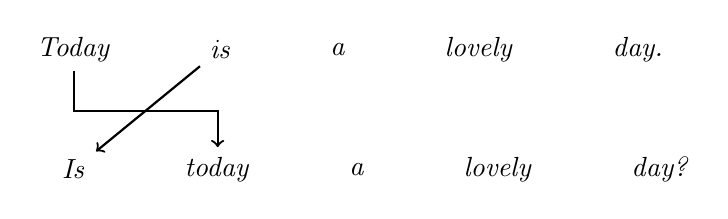
\begin{tikzpicture}[node distance=1cm]
    % Nodes for the declarative sentence
    \node (today1) {\textit{Today}};
    \node[right=of today1] (is1) {\textit{is}};
    \node[right=of is1] (a1) {\textit{a}};
    \node[right=of a1] (lovely1) {\textit{lovely}};
    \node[right=of lovely1] (day1) {\textit{day.}};

    % Nodes for the interrogative sentence
    \node[below=of today1] (is2) {\textit{Is}};
    \node[right=of is2] (today2) {\textit{today}};
    \node[right=of today2] (a2) {\textit{a}};
    \node[right=of a2] (lovely2) {\textit{lovely}};
    \node[right=of lovely2] (day2) {\textit{day?}};

    % Arrows
    \draw[->, thick] (is1) -- (is2) node [pos=0.5,left] {};
    \draw[->, thick] (today1.south) -- ++(0,-0.5) -| (today2.north);

\end{tikzpicture}
    \caption{The subject and the auxiliary verb \textit{is} switch places in the basic interrogative.}
    \label{fig:subj-aux-inversion}
\end{figure}

Not just any verb can participate in this inversion, only auxiliary verbs. In contemporary English, you can ask \textit{Are they going?} with the auxiliary verb \textit{are} in front of the subject \textit{they} but not *\textit{Go they?} with the lexical verb \textit{go} in front.\footnote{\textit{Go they} was possible until the end of the eighteenth century \citep[239]{Lass1999}.}

I introduced the auxiliary verbs in Section \ref{sec:aux} as those that have the NICER properties, and this kind of inversion is the \textit{I} in NICER (see Table \ref{tab:NICER2}).

\begin{table}
    \centering
    \begin{tabularx}{0.80\textwidth}{@{} >{\centering\arraybackslash\hsize=.03\hsize}X >{\hsize=.21\hsize}X >{\hsize=.38\hsize}X >{\hsize=.38\hsize}X @{}}
    \multicolumn{2}{>{\hsize=.24\hsize}X}{\textbf{Feature}} & \textbf{Examples} & \textbf{Counter-Examples} \\
    \hline
    \textbf{N} & egation:& \textit{Lee \uline{will} not eat.} & *\textit{Lee eats not.} \\
    \rowcolor{gray!20} % Apply background color here
    \textbf{I} & nversion:& \textit{Lee \uline{has} eaten.} \(\rightarrow\) \newline \textit{\uline{Has} Lee eaten?} & *\textit{Eats Lee?} \\
    \textbf{C} & ontraction:& \textit{didn't}, \textit{shouldn't} & *\textit{eatn't}, *\textit{keptn't} \\
    \textbf{E} & llipsis:& \textit{Kim \uline{was} eating, and \newline Lee \uline{was} ..., too.} & *\textit{Kim kept eating, and \newline Lee kept ..., too.} \\
    \textbf{R} & ebuttal:& \textit{I did tóo}/\textit{só read it.} \newline (\textit{Did not!}) & *\textit{I tried tóo}/\textit{só to read it.} (\textit{Tried not!}) \\
\end{tabularx}
\caption{The NICER properties}\label{tab:NICER2}
\end{table}

The other part of the inversion is the subject, which is introduced in Section \ref{sec:subjects}. There, I mentioned that \textsf{Subjects} typically precede the \textsf{Head} VP, but that in a basic interrogative (\textit{Could \uline{they} be right?}), the subject comes immediately after an auxiliary verb. \textsf{Subject}--auxiliary inversion is a key aspect of basic interrogatives, and that's actually kinda weird. Most languages don't make questions this way, and many English-language learners struggle with it. Instead of asking \textit{Is this right?} they'll ask \textit{This is right?} And of course, that's perfectly clear in most contexts, though, by default, it has the pragmatic force of requesting a clarification or expressing a doubt, rather than that of questioning.

\begin{tcolorbox}[title=Identifying the subject, colback=white, parbox]\label{box:finding-subject}
\setlength{\parindent}{1.5em}
    \noindent Sometimes, it's hard to find the subject. When you're stuck, alternating between a declarative and a basic interrogative can be helpful. Consider (\ref{ex:finding-subjects1} \& \ref{ex:finding-subjects2}).

    \ea \label{ex:finding-subjects1}
    \ea \textit{\uline{Tuesday} could be a good day to fly to Paris.}
        \ex \textit{Could \uline{Tuesday} be a good day to fly to Paris?}
        \z
    \z
    \ea \label{ex:finding-subjects2}
        \ea \textit{Tuesday, if things work out, \uline{you} could fly to Paris.}
        \ex \textit{Tuesday, if things work out, could \uline{you} fly to Paris?}
        \z
    \z

    In (\ref{ex:finding-subjects1}a), the first verb is the past-tense modal auxiliary \textit{could}. Modal auxiliaries don't have third-person singular forms, even in the present, and this is the past. As a result, agreement provides no clues about the subject. But in the basic interrogative in (\ref{ex:finding-subjects1}b), \textit{could} has moved in front of \textit{Tuesday}, which almost certainly means that \textit{Tuesday} is the subject.
    
    (\ref{ex:finding-subjects2}a) also lacks any agreement signals about the subject. But in the basic interrogative in (\ref{ex:finding-subjects2}b), \textit{could} is in front of \textit{you}, which means that \textit{Tuesday} \uline{cannot} be the subject; it must be \textit{you}.
    
\end{tcolorbox}

Here are some more examples with the auxiliary double underlined and the subject underlined. Those in (\ref{ex:befirstinterrogatives}) show different forms of auxiliary \textit{be}, those in (\ref{ex:modalfirstinterrogatives}) show different modal auxiliary verbs, and those in (\ref{ex:havefirstinterrogatives}) show two forms of auxiliary \textit{have} (as opposed to the lexical verb \textit{have}).
\ea \label{ex:befirstinterrogatives}
    \ea \textit{\uuline{Is} \uline{rain} ever warm?}
        \ex \textit{\uuline{Are} \uline{the evenings} sometimes too bright?}
        \ex \textit{\uuline{Am} \uline{I} functioning normally?}
        \ex \textit{Last night, \uuline{was} \uline{the moon}, perhaps, broken?}
    \z
\z
\ea \label{ex:modalfirstinterrogatives}
    \ea \textit{\uuline{Will} \uline{mornings} ever surprise you?}
        \ex \textit{\uuline{Could} \uline{silence} be too loud?}
    \z
\z
\ea\label{ex:havefirstinterrogatives}
    \ea \textit{In your experience, \uuline{have} \uline{dreams} lost their way?} 
    \ex \textit{\uuline{Had} \uline{the silent night} revealed its secrets before?} 
    \z
\z

You can see from these examples that, even with inversion, the auxiliary verb still agrees with the person and number of the subject, when possible: \textit{is} is the right form to agree with singular \textit{rain}, \textit{are} for plural \textit{the evenings}, and \textit{am} for first-person singular \textit{I}. 

I included (\ref{ex:befirstinterrogatives}d) to show that the auxiliary verb doesn't necessarily appear as the first element of the clause; other elements~-- the NP \textit{last night}, in this case~-- may come before it. The the auxiliary verb appears before the subject, but not always before everything. The same is true in (\ref{ex:havefirstinterrogatives}a): the auxiliary precedes the subject, but it still follows the PP \textit{in your experience}.


\subsection{\textit{Do} support}\label{sec:basic-do-support}

In all the examples so far, both the interrogative clauses and their corresponding declaratives would have an auxiliary verb. For example, the declarative counterpart of (\ref{ex:modalfirstinterrogatives}a) is \textit{Mornings \uline{will} {\op}sometimes{\cp} surprise you}, with the modal auxiliary verb \textit{will}. But lots of declarative clauses~-- perhaps most~-- don't have an auxiliary verb available for subject--auxiliary inversion. In such cases, we recruit \textit{do}, in its appropriate form. This is called \textsc{\textit{do} support}. 

If inverting the subject and the auxiliary to form a question is a bit odd, magically pulling some form of \textit{do} out of thin air and having it appear in front of the subject seems even stranger. It's no wonder language learners have problems with this. Nevertheless, it is the way we do it in Standard English, as you can see in (\ref{ex:basic-do-support}).

\ea \label{ex:basic-do-support}
    \ea \textit{\uuline{Do} \uline{coconuts} migrate?}
        \ex \textit{\uuline{Does} \uline{the Holy Grail} actually exist?}
        \ex \textit{\uuline{Did} \uline{Sir Robin} bravely run away?}
        \ex \textit{\uuline{Do} \uline{knights} prefer saying ``Ni'' to ``Hello''?}
        \ex \textit{\uuline{Does} \uline{the Norwegian Blue} pine for the fjords?}
    \z
\z

There's an extra step to watch out for here. The declarative counterpart of (\ref{ex:basic-do-support}b) would be \textit{The Holy Grail actually exist\uline{s}} with that third-person singular \textit{--s} on the present-tense verb. But in the basic interrogative, it's present-tense \textit{do} that agrees with the third-person singular, so \textit{do} \rightarrow \textit{does} and \textit{exist\uline{s}} \rightarrow \textit{exist}. Figure \ref{fig:do-support-s} shows this change under \textit{do} support with third-person, singular, present tense.

\begin{figure}
    \centering
    \begin{tikzpicture}[node distance=1cm]
    % Nodes for the declarative sentence
    \node (does1) {\phantom{does}};
    \node[right=of does1] (the1) {\textit{The}};
    \node[right=of the1] (holyGrail1) {\textit{Holy Grail}};
    \node[right=of holyGrail1] (actually1) {\textit{actually}};
    \node[right=of actually1] (exists1) {\textit{exist\uline{s}}};

    % Nodes for the interrogative sentence
    \node[below=of does1] (does2) {\textit{Do\uline{es}}};
    \node[below=of the1] (the2) {\textit{the}};
    \node[below=of holyGrail1] (holyGrail2) {\textit{Holy Grail}};
    \node[below=of actually1] (actually2) {\textit{actually}};
    \node[below=of exists1] (exist2) {\textit{exist}};

    % Arrows
    \draw[-{Latex[length=2mm]}] ([xshift=-1mm]does1.south) -- ([xshift=-1mm]does2.north) node[midway, right] {};
    \draw[-{Latex[length=2mm]}] ([xshift=3mm]exists1.south) -- ([xshift=5mm]does2.mid) node[midway, right] {};

\end{tikzpicture}
    \caption{\textit{Do} support with third-person, singular, present-tense.}
    \label{fig:do-support-s}
\end{figure}

\noindent Figure \ref{fig:do-support-d} shows \textit{do} support with past tense. Again, the tense is marked on \textit{do} and not on the lexical verb.

\begin{figure}
    \centering
    \begin{tikzpicture}[node distance=1cm]
    % Nodes for the declarative sentence
    \node (does1) {\phantom{does}};
    \node[right=of does1] (the1) {\textit{The}};
    \node[right=of the1] (holyGrail1) {\textit{Holy Grail}};
    \node[right=of holyGrail1] (actually1) {\textit{actually}};
    \node[right=of actually1] (exists1) {\textit{exist\uline{ed}}};

    % Nodes for the interrogative sentence
    \node[below=of does1] (does2) {\textit{Di\uline{d}}};
    \node[below=of the1] (the2) {\textit{the}};
    \node[below=of holyGrail1] (holyGrail2) {\textit{Holy Grail}};
    \node[below=of actually1] (actually2) {\textit{actually}};
    \node[below=of exists1] (exist2) {\textit{exist}};

    % Arrows
    \draw[-{Latex[length=2mm]}] ([xshift=-1mm]does1.south) -- ([xshift=-1mm]does2.north) node[midway, right] {};
    \draw[-{Latex[length=2mm]}] ([xshift=3mm]exists1.south) -- ([xshift=5mm]does2.mid) node[midway, right] {};

\end{tikzpicture}
    \caption{\textit{Do} support with past tense.}
    \label{fig:do-support-d}
\end{figure}

\begin{tcolorbox}[title=A verb-form puzzle, colback=white, parbox]\label{box:puzzle-1}
\setlength{\parindent}{1.5em}
    \noindent 
    In \textit{Does the Holy Grail actually exist}, isn't \textit{exist} also present tense? So, shouldn't it also agree? In fact, \textit{exist} is the plain form of the verb: there is only one tensed verb in this clause and that's \textit{do}(\textit{es}). This is surprisingly difficult to show, and I can't think of a way to do it with a basic interrogative, but I'll return to the issue after discussing focused interrogatives (Section \ref{box:puzzle-2}). In the mean time, try to think it through.
\end{tcolorbox}

\subsection{Semantics}\label{sec:question-semantics}

Basic interrogatives are usually used to ask closed questions.\footnote{Again, \textit{CGEL} uses \textsc{closed interrogative} for the syntactic construction I'm calling the \textsc{basic interrogative}.} One kind of closed question is the \textit{yes}/\textit{no} question. If I ask you, \textit{Is rain ever warm?} then I basically expect you to either confirm or deny that rain is at least sometimes warm. You could say, \textit{Yes, it is}, or \textit{Sometimes}, or \textit{I think so}, but \textit{Aardvark} is not an answer. \textit{I don't know} may be a valid \textsc{response}, but it too doesn't qualify as a \textsc{answer}. So, such a question has a \textbf{closed} set of answers that, specific wording aside, boil down to `yes' or `no'. 

Another kind of closed question offers a set of alternatives. For example, \textit{Would you like to eat at 5:30, 7:00, or 7:30?} closes the set of answers to one of those three times. Pragmatically, you could respond with indifference, express a love for food, comment on other obligations you have, suggest another time, or decline the offer of dinner altogether. But strictly within the semantic framework, none of those responses qualify as direct answers. The only ones that count as answers are those that state or imply a preference for one of the three times.

\begin{figure}
    \centering
    \includegraphics[width=0.5\linewidth]{figures/closedInterrogativesMeme.jpg}
    \caption{Two types of closed questions.}
    \label{fig:closed-int-meme}
\end{figure}

And on the topic of semantics, I would remind you that, syntactically, basic \uline{interrogative} clauses are not always semantically \uline{questions}. They can also be exclamations (\textit{Isn't this the best cake you've ever tasted?}), expressions of surprise (\textit{Are you serious?}), insults (\textit{Did an infant dress you?}), advice (\textit{Wouldn't it be better to read the instructions?}), and so on. So, while the structure may be interrogative, the intended meaning can diverge from straightforward questioning.

\subsection{Intonation}

In most Standard English dialects, yes/no questions typically have a rising intonation, while alternative questions fall on the final alternative after rising on each previous one, as shown in Figure \ref{fig:question-intonation}.

\begin{figure}
    \centering
    \begin{tikzpicture}
    % Yes/No Question
    \node[align=left] (ynq) {\textit{Is rain ever warm?}};
    \draw[thick, -{Latex[bend]}] (ynq.east) to [bend right] ++(0.3,0.5);

    % Alternative Question
    \node[align=right, below=0.5cm of ynq] (aq) {\phantom{Woul}\textit{Would you like to eat at}};
    \node[align=center, right=-6pt of aq] (time1) {\textit{5:30,}};
    \node[align=center, right=0pt of time1] (time2) {\textit{7:00,}};
    \node[align=center, right=0pt of time2] (time3) {\textit{or 7:30?}};
    
    % Arrows for alternative question
    \draw[thick, -{Latex[bend]}] ([xshift=-2pt]time1.east) to [bend right] ++(0.3,0.5);
    \draw[thick, -{Latex[bend]}] ([xshift=-2pt]time2.east) to [bend right] ++(0.3,0.5);
    \draw[thick, -{Latex[bend]}] ([xshift=-2pt]time3.east) to [bend left] ++(0.3,-0.5);
    
\end{tikzpicture}
    \caption{Typical intonation in \textit{yes}/\textit{no} and alternative questions.}
    \label{fig:question-intonation}
\end{figure}

This can vary quite a bit though, depending on the attitude behind the question (mere curiosity, doubt, anger, etc.), whether it is said in isolation or as one a series of questions, and various other factors \citep{Bartels1999}.

\section{Focused interrogative clauses}\label{sec:focused interrogatives}

Focused interrogatives typically start with an \textsc{interrogative word}: \textit{who} (including \textit{whose} and with decreasing frequency \textit{whom}), \textit{what}, \textit{which}, \textit{when}, \textit{where}, \textit{why}, or \textit{how}.\footnote{There are also some older or archaic words that students don't need to learn, including \textit{whence}, \textit{whither}, and some compound prepositions such as \textit{whereby} and \textit{wherein}.} This is an important group of words, a group that has a central syntactic role in forming interrogative phrases and clauses and a central semantic role in asking questions. But \textsc{interrogative word} isn't a lexical category like pronoun or auxiliary verb; interrogative words belong to many different lexical categories, as shown in Table \ref{tab:q-words}. (Did you notice which category/ies is/are not represented?)

\begin{table}[h]
    \centering
    \begin{tabular}{ll}
        \hline
        \textbf{Lexical Category} & \textbf{Interrogative words} \\
        \hline
        Pronoun & \textit{who}/\textit{whose}/\textit{whom} \\
        Determinative & \textit{what} \& \textit{which} \\
        Preposition & \textit{where} \& \textit{when} \\
        Adverb & \textit{why} \& \textit{how}\\
        Adjective & \textit{how}   \\
        \hline
        \end{tabular}
    \caption{Lexical categories of interrogative words (based on \textit{CGEL})} \label{tab:q-words}
\end{table}

\subsection{Interrogative phrases} \label{sec:interrogative-phrases}
The interrogative words appear in \textsc{interrogative phrases}, such as those underlined in (\ref{ex:int-phrases}). Sometimes they're the \textsf{Head} and the only word in the phrase, as in (\ref{ex:who-s-the-kid}), where \textit{who} is the \textsf{Head} of an NP. Sometimes they're the \textsf{Head} along with one or more \textsf{Dependents}, as in (\ref{ex:precisely-who}). And sometimes, they are a \textsf{Dependent} somewhere in a larger phrase, as in (\ref{ex:what-time}) and (\ref{ex:at-what-time}). In both, \textit{what} functions as the \textsf{Determiner} in the NP \textit{what time}, but in (\ref{ex:at-what-time}), the interrogative phrase is the whole \textit{at} PP, which includes the NP, which, in turn, includes \textit{what}.

\ea
    \ea{\textit{\uline{Who}'s the kid?}}\label{ex:who-s-the-kid}
    \ex{\textit{\uline{Precisely who} called you?}}\label{ex:precisely-who}
    \ex{\textit{\uline{What time} did they arrive?}}\label{ex:what-time}
    \ex{\textit{\uline{At what time} did they arrive?}}\label{ex:at-what-time}
    \z\label{ex:int-phrases}
\z

Common interrogative phrases, apart from the individual words already listed include \textit{how many}, \textit{how often}, \textit{how long}, \textit{what day}, and \textit{since when}. There are also a number with \textit{how} that are semantically interrogative but function syntactically unlike the others. These include \textit{\uline{How come} you did that?}, \textit{\uline{How about} if we take a break?}, \textit{\uline{What about} this one?} 

Interrogative phrases work very well as questions all on their own, given the right context. If somebody says, ``they're arriving tomorrow,'' then \textit{What time?} is a perfectly reasonable way to ask what time they are arriving.

\subsection{Interrogative phrase subjects}\label{sec:focussed-subj}

Cases like (\ref{ex:he->who}) are the easiest. \textit{Who} is a pronoun that is the \textsf{Head} of an NP, and that NP functions as the subject of the focused interrogative clause. Starting with \textit{He's the kid}, we just replace \textit{he} with \textit{who}, and we're done.

    \ea{\textit{\uline{He}'s the kid.} \rightarrow~\textit{\uline{Who}'s the kid?}}\label{ex:he->who}
    \z
And, as long as the interrogative phrase is the subject, then focused interrogative clauses work like this. (\ref{ex:int-phr-subj}) shows various such examples.

\begin{exe}
    \ex
    \begin{xlist}
        \ex 
        \begin{tabular}[t]{@{}p{4.1cm}@{}p{6cm}@{}}
            \textit{\uline{That} smells.} & \(\rightarrow\) \textit{\uline{What} smells?}
        \end{tabular}
        
        \ex 
        \begin{tabular}[t]{@{}p{4.1cm}@{}p{6cm}@{}}
            \textit{\uline{This time} works for me.} & \(\rightarrow\) \textit{\uline{Roughly what time} works for you?}
        \end{tabular}
        
        \ex 
        \begin{tabular}[t]{@{}p{4.1cm}@{}p{6cm}@{}}
            \textit{\uline{Nobody} can come.} & \(\rightarrow\) \textit{\uline{Which of your friends} can come?}
        \end{tabular}
        
        \ex \label{ex:person-people}
        \begin{tabular}[t]{@{}p{4.1cm}@{}p{6cm}@{}}
            \textit{\uline{One person} was there.} & \(\rightarrow\) \textit{\uline{How many people} were there?}
        \end{tabular}
    \end{xlist}
    \label{ex:int-phr-subj}
\end{exe}

Notice that in (\ref{ex:person-people}), the question is asked in the plural.

\subsection{Subject--auxiliary inversion and fronting} \label{sec:subj-aux-inversion-and-fronting}

But it's not always the case that the interrogative phrase is the subject. When it's not, we're back to subject--auxiliary inversion and sometimes \textit{do} support, as with the basic interrogatives. And again, this can cause difficulties for students, who often produce uninverted clauses. The inversion is shown in (\ref{ex:when-was-it-there}).

\ea \label{ex:when-was-it-there}
    \ea{\textit{\phantom{Wh is it }\textbf{It} is \uline{a pen}.}}\label{ex:when-was-it-there-a}
    \ex{\textit{\phantom{Wh is it }\textbf{It} is \uline{what}?}}\label{ex:when-was-it-there-b}
    \ex{\textit{\uline{What} is \textbf{it} \phantom{ is}  \uline{\phantom{what}}?}\hfill[fronted]}\label{ex:when-was-it-there-c}
    \z
\z

There are a few things to observe here. First, \textit{it} functions as the subject in all three examples, even when it's the last word in the clause. Second, \textit{a pen} functions as a complement in the VP in the declarative (\ref{ex:when-was-it-there-a}), as does \textit{what} in (\ref{ex:when-was-it-there-b}). And then there's the fronted interrogative phrase in (\ref{ex:when-was-it-there-c}).\footnote{I mentioned fronting and stranding back in Section \ref{sec:preposition-stranding}.} That phrase is now in what we'll call \textsc{Pre function} (see Section \ref{sec:phrase-structure}), the auxiliary verb is before the subject, and there's just an empty space where the complement in the VP used to be. I'm going to claim that there really is a gap there, and its function really is the same as that of \textit{a pen} in (a): it's still a complement. See (\ref{ex:int-phr-inversion}) for a few more examples.

\begin{exe}
    \ex
    \begin{xlist}
        \ex 
        \begin{tabular}[t]{@{}p{4.4cm}@{}p{6cm}@{}}
            \textit{They can't smell \uline{it}.} & \(\rightarrow\) \textit{\uline{What} can't they smell \uline{\phantom{it}}?}
        \end{tabular}
        
        \ex 
        \begin{tabular}[t]{@{}p{4.4cm}@{}p{6cm}@{}}
            \textit{I'm free \uline{until 5:00}.} & \(\rightarrow\) \textit{\uline{Until when} are you free \uline{\phantom{until 5:00}}?}
        \end{tabular}
        
        \ex 
        \begin{tabular}[t]{@{}p{4.4cm}@{}p{6cm}@{}}
            \textit{I should see \uline{these} then.} & \(\rightarrow\) \textit{\uline{Which} should you see \uline{\phantom{them}} then?}
        \end{tabular}
        
        \ex 
        \begin{tabular}[t]{@{}p{4.4cm}@{}p{6cm}@{}}
            \textit{It might be bad \uline{since I lost}.} & \(\rightarrow\) \textit{\uline{Why} might it be bad \uline{\phantom{since I lost}}?}
        \end{tabular}

        \ex 
        \begin{tabular}[t]{@{}p{4.4cm}@{}p{6cm}@{}}
            \textit{I will want \uline{you} to do it.} & \(\rightarrow\) \textit{\uline{Who} will you want \uline{\phantom{you}} to do it?}
        \end{tabular}

        \ex \label{ex:how-can-I}
        \begin{tabular}[t]{@{}p{4.4cm}@{}p{6cm}@{}}
            \textit{You can do it \uline{like this}.} & \(\rightarrow\) \textit{\uline{How} can I do it \uline{\phantom{like this}}?}
        \end{tabular}

        \ex \label{ex:about-what}
        \begin{tabular}[t]{@{}p{4.4cm}@{}p{6cm}@{}}
            \textit{I was speaking \uline{to him}.} & \(\rightarrow\) \textit{Uh, \uline{who} was I speaking to \uline{\phantom{him}}?}
        \end{tabular}
    \end{xlist}
    \label{ex:int-phr-inversion}
\end{exe}

As exemplified in (\ref{ex:how-can-I}), when using singular \textit{you} or \textit{I}, the declarative and the interrogative typically have contrasting pronouns: I ask about you and you answer \textit{I}, I ask about myself and you answer \textit{you}. For this reason, unless you're making this specific point, I avoid \textit{you}/\textit{I} examples when explaining interrogatives. That said, as (\ref{ex:about-what}) shows, sometimes we speak to ourselves.

(\ref{ex:about-what}) is also another example of PP fronting. Notice that all the other examples in (\ref{ex:int-phr-inversion}) have interrogative phrases that start with (and are limited to) an interrogative word. Only the interrogative PP \textit{about what} starts with a non-interrogative word.

    \begin{tcolorbox}[title=Practice, colback=white, parbox]
        \setlength{\parindent}{1.5em}
        \noindent 
        Identify an interrogative phrase that would result in the given answer, and state its function in the interrogative clause. See the example.

        \phantom{x}

        Example: \textit{Brett wrote it.}\\
        \phantom{xxx}Interrogative phrase: \uline{\textsf{\textit{who}}}, function: \uline{\textsf{\textit{Subject}}}\\
        \phantom{xxx}Explanation: One likely question is \textit{\uline{Who} wrote this book?} (See Section \ref{sec:focussed-subj})

        \begin{enumerate}[noitemsep]
            \item Answer: \textit{I'm from Toronto.}\\
            Interrogative phrase: \uline{\phantom{xxxxxxxxxx}}, function: \uline{\phantom{xxxxxxxxxx}}
            
            \item Answer: \textit{I usually go to bed around 11 PM.}\\
            Interrogative phrase: \uline{\phantom{xxxxxxxxxx}}, function: \uline{\phantom{xxxxxxxxxx}}

            \item Answer: \textit{Taylor did.}\\
            Interrogative phrase: \uline{\phantom{xxxxxxxxxx}}, function: \uline{\phantom{xxxxxxxxxx}}

            \item Answer: \textit{I bought it last week.}\\
            Interrogative phrase: \uline{\phantom{xxxxxxxxxx}}, function: \uline{\phantom{xxxxxxxxxx}}

            \item Answer: \textit{She went to the library.}\\
            Interrogative phrase: \uline{\phantom{xxxxxxxxxx}}, function: \uline{\phantom{xxxxxxxxxx}}

            \item Answer: \textit{He's feeling much better now.}\\
            Interrogative phrase: \uline{\phantom{xxxxxxxxxx}}, function: \uline{\phantom{xxxxxxxxxx}}

            \item Answer: \textit{I gave it to Jean.}\\
            Interrogative phrase: \uline{\phantom{xxxxxxxxxx}}, function: \uline{\phantom{xxxxxxxxxx}}

            \item Answer: \textit{The tickets were \$20.}\\
            Interrogative phrase: \uline{\phantom{xxxxxxxxxx}}, function: \uline{\phantom{xxxxxxxxxx}}

            \item Answer: \textit{Don't worry, it's my phone}.\\
            Interrogative phrase: \uline{\phantom{xxxxxxxxxx}}, function: \uline{\phantom{xxxxxxxxxx}}

            \item Answer: \textit{She's an architect.}\\
            Interrogative phrase: \uline{\phantom{xxxxxxxxxx}}, function: \uline{\phantom{xxxxxxxxxx}}

            \item Answer: \textit{They visited Paris last summer.}\\
            Interrogative phrase: \uline{\phantom{xxxxxxxxxx}}, function: \uline{\phantom{xxxxxxxxxx}}

            \item Answer: \textit{I read about it in the newspaper.}\\
            Interrogative phrase: \uline{\phantom{xxxxxxxxxx}}, function: \uline{\phantom{xxxxxxxxxx}}


        \end{enumerate}
    \end{tcolorbox}

\subsection{\textit{Do} support inversion}\label{sec:focused-do-support}

Just as with basic interrogatives, subject--auxiliary inversion works fine with focused interrogatives when there is an auxiliary in the corresponding declarative. But when there isn't, then we once again lean on \textit{do} for support. See (\ref{ex:int-phr-do}) for a few more examples.

\begin{exe}
    \ex
    \begin{xlist}
        \ex \label{ex:int-phr-do-a}
        \begin{tabular}[t]{@{}p{4.3cm}@{}p{6cm}@{}}
            \textit{They smelled \uline{it}.} & \(\rightarrow\) \textit{\uline{What} \textbf{did} they smell \uline{\phantom{it}}?}
        \end{tabular}
        
        \ex \label{ex:int-phr-do-b}
        \begin{tabular}[t]{@{}p{4.3cm}@{}p{6cm}@{}}
            \textit{I get free \uline{after 5:00}.} & \(\rightarrow\) \textit{\uline{When} \textbf{do} you get free \uline{\phantom{after 5:00}}?}
        \end{tabular}
        
        \ex 
        \begin{tabular}[t]{@{}p{4.3cm}@{}p{6cm}@{}}
            \textit{I see \uline{them} then.} & \(\rightarrow\) \textit{\uline{Who} \textbf{do} you see \uline{\phantom{them}} then?}
        \end{tabular}
        
        \ex 
        \begin{tabular}[t]{@{}p{4.3cm}@{}p{6cm}@{}}
            \textit{It seems bad \uline{since I lost}.} & \(\rightarrow\) \textit{\uline{Why} \textbf{does} it seem bad \uline{\phantom{since I lost}}?}
        \end{tabular}

        \ex 
        \begin{tabular}[t]{@{}p{4.3cm}@{}p{6cm}@{}}
            \textit{It looks \uline{good}.} & \(\rightarrow\) \textit{\uline{How} \textbf{does} it look \uline{\phantom{good}}?}
        \end{tabular}
    \end{xlist}
    \label{ex:int-phr-do}
\end{exe}

And, just like before, the tense moves from the lexical verb to \textit{do}, and the lexical verb appears in the plain form. For example, in (\ref{ex:int-phr-do-a}), past-tense \textit{smelled} becomes plain-form \textit{smell}, and past-tense \textit{did} is used. Similarly, in (\ref{ex:int-phr-do-b}), present-tense \textit{get} becomes plain-form \textit{get}, only this time, the forms share a shape, so the change is surreptitious.


\begin{tcolorbox}[title=A verb-form puzzle, colback=white, parbox] \label{box:puzzle-2}
\setlength{\parindent}{1.5em}
    \noindent 
Earlier (Section \ref{box:puzzle-1}), I brought up the question of whether or not \textit{exist} is present tense in \textit{Does the Holy Grail actually exist?} Now, I can use an interrogative to show you that it's clearly the plain form.

\ea \label{ex:WDYbe}
    \ea[]{\textit{The cat's \uline{is} very loud.}}
        \ex[*]{\textit{Does it ever just \uline{is} quiet?}}
        \ex[]{\textit{Does it ever just \uline{be} quiet?}}
    \z
\z

If we try to use the present-tense form of \textit{be}, the result is the ungrammatical (\ref{ex:WDYbe}b). It's the plain-form \textit{be} in (c) that is correct. The reason this is so difficult to show is that \textit{be} is the only verb that has a plain form that is distinct from the plain present-tense form.

\end{tcolorbox}


Finally, there's the special case of asking about an activity, as in (\ref{ex:activity-question}). In such cases, since the speaker, who may or may not know what the activity is/was, assumes that the listener knows, we use lexical~-- not auxiliary~-- \textit{do} as a stand-in for the activity. The structure, though, is the same. (\ref{ex:what-did}) exhibits \textit{do} support~-- auxiliary \textit{did} together with lexical \textit{do}~-- (\ref{ex:what-modal}) shows subject--auxiliary inversion with modal auxiliaries, and (\ref{ex:what-are}) does the same but with the progressive aspect, as does (\ref{ex:what-have}) with perfect aspect.

\ea\label{ex:activity-question}
    \ea{\textit{What did you \uline{do}?}}\label{ex:what-did}
    \ex{\textit{What might}/\textit{can}/\textit{will you \uline{do}?}}\label{ex:what-modal}
    \ex{\textit{What are}/\textit{were you \uline{doing}?}}\label{ex:what-are}
    \ex{\textit{What have}/\textit{had you \uline{done}?}}\label{ex:what-have}
    \z
\z

\subsection{Summary}
So in sum, there are three different types of interrogatives. A decision tree is set out in Figure \ref{fig:decision-tree}.

\begin{figure}
    \centering
    \begin{forest}
        for tree={align=center, parent anchor=south, child anchor=north, l=1.25cm, s sep=1cm, edge={->,thick}}
        [Is there an interrogative phrase?
            [Yes \\\textit{Focused}\\ Is the interrogative phrase the subject?
                [Yes \\ \textit{Non-inverting}]
                [No \\ \textit{Inverting} \\ Does the declarative have an auxiliary verb?, name=does
                    [Yes \\ \textit{Use subject--auxiliary inversion}]
                    [No \\ \textit{Use \textsc{\textit{do}} support}]
                ]
            ]
            [No \\\textit{Basic}, name=auxfirst
            ]
        ]
        % Drawing an arrow from "No basic" to a new node
        % Adding options below the new node
        %\node [below left=of auxverb, align=center] (yesaux) {Yes \\ \textit{Use subject--auxiliary inversion}};
        %\node [below right=of auxverb, align=center] (noaux) {No \\ \textit{Use \textit{do} support}};
        %\draw[->, thick] (auxverb.south) -- (yesaux.north);
        %\draw[->, thick] (auxverb.south) -- (noaux.north);
    \end{forest}
    \caption{The choice between interrogative structures.}
    \label{fig:decision-tree}
\end{figure}

\subsection{Semantics}

It will be familiar by now that interrogatives can do more than ask questions, but, in general, the focused interrogatives are used to ask \textsc{open questions}.\footnote{CGEL uses the term \textit{open interrogatives} for focused interrogatives, which typically ask open questions.} These are open in that, when you ask, \textit{who did you see?} for example, the answer is limited only by the requirement that it be a person or persons. Otherwise, the possibilities are open. The main exception to this is \textit{which}, which expects answers from a closed set, sometimes explicit (e.g., \textit{Which would you like, small, medium, or large?}) and sometimes inferrable from the context (e.g., \textit{Which one looks best?}).

\subsection{Intonation}

In general, open questions (and therefore most focused interrogative clauses) end with falling intonation.

\section{Questions in the classroom and classroom questions}

Even before students start learning the ins and outs of English interrogative clauses, they're able to ask questions: simple interrogative phrases, like \textit{how long?} for \textit{How long will it take?} or declarative clauses with rising intonation, such as \textit{We have a test?} for \textit{Do we have a test?} 

The first is perfectly natural and accurate, and should not be met with an injunction to ``use complete sentences.'' Usually, if the student has chosen an interrogative-phrase question, a complete sentence would contain awkward redundancy, making the asker appear stiff and foreign. In the second case though, the student's high-terminal declarative is inappropriate, unless the teacher has already said something about a test. That's because the speech act evoked from such a clause is not a straight-forward closed question. Rather, it's a request for confirmation, clarification, or restatement. The distinction is subtle, but consider Person A's second turn in (\ref{ex:confirmation-questions}).

\ea \label{ex:confirmation-questions}
    \textbf{Person A}: \textit{I saw a poster about that concert you mentioned last week.} \\
    \textbf{Person B}: \textit{Oh, the one at the park? Yeah, the whole team's going.} \\
    \textbf{Person A}: \textit{You're going?} \\
    \textbf{Person B}: \textit{Yeah, do you want to come?} \\
\z

 \textit{You're going?} is a request to clarify whether `the team' includes Person B. The question \textit{Are you going?} might suggest A wasn't paying attention because, from Person B's viewpoint, they've just told A they're going. By framing the question as a declarative, A acknowledges this possibility while asking for clarification. In other words, high-terminal declaratives have their place, but it's not a general question-asking form, and students should understand the difference.

 There's one more common questioning strategy that students use. The clauses covered in this chapter are main clauses, but students sometimes employ subordinate interrogative clauses (See Section  ?????) as questions. For example, a student may ask, pointing, \textit{how to say this word?} This is a subordinate interrogative clause, and as such, it's perfectly fine inside another clause~-- \textit{Could you tell me~\uline{how to say this word}?} or \textit{I wonder~\uline{how to say this word}.}~-- but it's not Standard to use such clauses on their own to ask questions. Instead we'd use a focused interrogative with \textit{do} support: \textit{How do you say this word?}

\begin{tcolorbox}[title=Classroom Questions, colback=white, parbox]
\setlength{\parindent}{1.5em}
    \noindent A good way to start learning how to ask questions is to memorize some, and a good set to memorize is the set of questions that come up in the language classroom regularly. Here are some ideas, but I'm sure you can think of others.

 \begin{enumerate}[noitemsep]
    \item \textit{What does \uline{\phantom{MMM}} mean?}
    \item \textit{How do you spell \uline{\phantom{MMM}}?}
    \item \textit{How do you say this/that word?} (pointing)
    \item \textit{How do you say }[first-language word]\textit{ in English?}
    \item \textit{Can you give me an example?}
    \item \textit{Is this OK?}
    \item \textit{Can I say \uline{\phantom{MMM}}?}
    \item \textit{Do you have a \uline{\phantom{MMM}}?}
    \item \textit{Can I borrow a \uline{\phantom{MMM}}?}
    \item \textit{Do we have any homework?}
    \item \textit{When is it due?}
    \item \textit{Did I spell this right?}
    \item \textit{Why do we use this tense here?}
    \item \textit{What's the past tense of \uline{\phantom{MMM}}?}
    \item \textit{What's your email address?}
    \item \textit{When do we use \uline{\phantom{MMM}}?}
    \item \textit{Could you repeat that, please?}
    \item \textit{What's the difference between \uline{\phantom{MMM}} and \uline{\phantom{MMM}}?}
    \item \textit{Where can I find out more about \uline{\phantom{MMM}}?}
    \item \textit{What should we do next?}
\end{enumerate}
\end{tcolorbox}

\section{Phrase structure}\label{sec:phrase-structure}

\subsection{Basic interrogatives with subject--auxiliary inversion}
Trees may help you think about the structure of basic interrogatives. The tree for the basic interrogative clause \textit{Could they be right?} is shown in Figure \ref{fig:tree-theycouldberight}.

\begin{figure}[htb]
  \centering
  \begin{subfigure}[b]{0.48\textwidth}
    \centering
    \includegraphics[width=\textwidth]{figures/couldtheyberight.pdf}
    \caption{\textit{Could they be right}: \textsf{Subj}--aux inversion.}
    \label{fig:tree-theycouldberight}
  \end{subfigure}
  \hfill
  \begin{subfigure}[b]{0.48\textwidth}
    \centering
    \includegraphics[width=.91\textwidth]{figures/do-you-like-tree.pdf}
    \caption{\textit{Do you like pizza}, with \textit{do} support.}
    \label{fig:do-you-like}
  \end{subfigure}
  \caption{Syntax trees for basic interrogatives.}
  \label{fig:combined-trees}
\end{figure}
%\begin{forest}
%where n children=0{% for each terminal node
%    font=\itshape, 			% italics
%    tier=word          			% align at the "word" tier (bottom)
%  }{%								% no false conditions, so empty
%  },
%[Clause
%	[\Node{Prenucleus}{V\textsubscript{\textsc{aux }x}}[could]]
%	[\Head{Clause}
%		[Section ubj{NP}[they, roof]]
%		[\Head{VP}
%			[\Head{GAP\textsubscript{x}}[--]]
%			[\Comp{Clause}[be right, roof]]
%		]
%	]
%]
%\end{forest}

The first thing to notice about the trees is the \textit{x} subscripts after V\textsubscript{\textsc{aux}} and GAP. Linguists call such a mark a \textsc{co-index}. It's called a \uline{co-}index because it's shared between two (or more) elements, and it's called a co-\uline{index} because, like an index in the back of the book, it points you to something you want to find: if you're wondering where \textit{could} came from, you check the index, and it tells you it came from the position that now says GAP.

The next notable element is the GAP itself, which is a placeholder. The VP, like all phrases, needs a \textsf{Head}, but in this case, the \textsf{Head} is the GAP that's co-indexed to \textit{could}, rather than being a verb, as we would usually expect for the \textsf{Head} of a VP. Such GAPs are more important for linguistic theory than for language teaching, but as we see more gaps in this chapter and others that follow, I expect you'll come to see them as important and useful tools for your own thinking about phrase structure.

Having looked at these two crucial elements, let's go through the tree on the left as a review. Starting at the top, we see that it has an auxiliary verb \textit{could} in \textsf{Prenucleus} function, which is the key element of the basic interrogative clause type. Since \textit{prenucleus} is an ugly, ponderous word used by virtually nobody outside the \textit{CGEL} framework, I will simply call it \textsc{Pre} from now on (there will be a \textsc{Post} later). Be sure to understand that subject--auxiliary inversion does not mean that the subject somehow becomes the auxiliary and vice versa. As the tree shows, the subject remains the subject, and the auxiliary verb appears in the \textsf{Pre} function.

%make sure to introduce Post or remove this

Next, there is the \textsf{Head} clause \textit{they~-- be right}. At first glance, it may seem strange to have a clause as the \textsf{Head} of another clause. But this is an essential aspect of understanding basic interrogatives. In our example, the main clause functions as the \textsf{Head} of the overall interrogative structure. This arrangement is due to the unique positioning of \textit{could} in \textsf{Pre} function. It has to be pre-something, and this shows it as preceding the central clause.

In the tree, the \textsf{Head} clause includes a subject NP (\textit{they}) and a \textsf{Head} VP, represented by the GAP (--) where \textit{could} would normally be. The clause \textit{be right} acts as a \textsf{Complement}, and its internal structure is simplified as a triangle here. I encourage you to sketch this tree yourself to grasp its structure fully. Compare your version with Figure \ref{fig:tree-theycouldberight}, and don't be discouraged if you miss some elements initially. Practice will help you capture all the components accurately.

\subsection{Basic interrogatives with \textit{do} support}

A tree with \textit{do} support looks, structurally, just like one with subject-auxiliary inversion, such as the tree in Figure \ref{fig:tree-theycouldberight}. The tree for the basic interrogative \textit{Do you like pizza?} is shown in Figure \ref{fig:do-you-like}. Again, the auxiliary verb \textit{do} is in \textsf{Pre} function, again the rest of the clause follows as the \textsf{Head}, and again, there's a GAP in the VP.



\subsection{Focused interrogatives with subject focus}

Next is the focused interrogative. Again, we'll start with the easiest case, the one with the interrogative phrase as the subject. The example in Figure \ref{fig:who-plays} is \textit{Who plays the piano?} There's no \textsf{Pre} and no gap, just \textit{who} functioning as the subject. It couldn't be easier, and English language learners rarely make mistakes with this clause structure.


\begin{figure}[htbp]
  \centering
  \begin{subfigure}[b]{0.48\textwidth}
    \centering
    \includegraphics[width=.75\textwidth]{figures/who-plays-tree.pdf}
    \caption{Tree for \textit{who plays the piano}.}
    \label{fig:who-plays}
  \end{subfigure}
  \hfill
  \begin{subfigure}[b]{0.48\textwidth}
    \centering
    \includegraphics[width=\textwidth]{figures/what-can-you-tree.pdf}
    \caption{Tree for \textit{what can you play}.}
    \label{fig:what-can-you}
  \end{subfigure}
  \caption{Syntax trees for focused interrogatives.}
  \label{fig:combined-trees2}
\end{figure}


%\begin{forest}
%  for tree={
%    l=0.5cm, % Adjusts the level distance
%    s=12cm, % Adjusts the sibling distance
%  },
%where n children=0{% for each terminal node
%    font=\itshape, 			% italics
%    tier=word          			% align at the "word" tier (bottom)
%  }{%								% no false conditions, so empty
%  },
%[Clause
%	[\Node{Pre}{NP\textsubscript{x}}[what, roof]]
%	[\Head{Clause}
%		[\Node{Pre}{V\textsubscript{\textsc{aux }y}}[can]]
%		[\Head{Clause}
%			[Section ubj{NP}[you, roof]]
%			[\Head{VP}
%				[\Head{GAP\textsubscript{y}}[--]]
%				[\Comp{Clause}
%					[\Head{VP}
%						[\Head{v}[play]]
%						[\Obj{GAP\textsubscript{x}}[--]]
%					]
%				]	
%			]
%		]
%	]
%]
%\end{forest}

\subsection{Focused interrogatives with non-subject focus}

When the interrogative phrase (i.e, the focus) is not the subject, then things get more complex and language learners are much more likely to form questions lacking inversion, like \textit{What you can play?} In \textit{What can you play?} in Figure \ref{fig:what-can-you}, there are two constituents in \textsf{Pre} function, two gaps, and two different co-indices \textit{x} and \textit{y}. Each co-index connects the \textsf{Pre} to its relevant gap. 

The functions of the gaps are clearer here. \textit{Play} is a transitive verb, the kind that takes an \textsf{Object}, so there's an \textsf{Object} gap. While we might say informally that \textit{what} is the \textsf{Object} of \textit{play}, that would go against the idea that an \textsf{Object} is a \textsf{Dependent} in the VP, so we give \textit{what} a different function (\textsf{Pre}) but connect it back to the \textsf{Object} through the \textit{x} co-index.

%\chapter{Negation}

\epigraph{We would not say, ``I don't have it.''
Instead, we say, ``It hasn't yet come to me.'' That difference
is everything.}{}

\is{negation|(}Negation is a topic that seems extremely simple on the surface, but its underlying complexity makes it a great vehicle for understanding so many areas of the language landscape: \is{scope|(}scope, \is{polarity (positive vs negative)|(}polarity, \is{language change|(}language change, \is{grammaticalization|(}grammaticalization, and \is{exaptation}exaptation.

\section{Language change, grammaticalization, and exaptation}

``I heard not of it before,'' says Bertram in Shakespeare's \textit{All's well that ends well}. You and I would say \textit{I have not heard of it before}.

Language~-- as you can clearly see~-- changes. But the changes are often surprisingly systematic.

\il{English!Old|(}Old English (450--1150 CE) used \textit{ne}, simply placed before the verb, for negation. Take (\ref{ex:ne-habbe}) for example.

\ea \label{ex:ne-habbe}
    \gll \textit{Ne} \textit{hæbbe} \textit{ic} \textit{hit} \textit{ær} \textit{gehīered} \\ no(t) have I it before {heard of} \\
    \trans `I have not heard of it before.'
\z

If things had stayed this way,\footnote{Actually, there is a construction in which things more or less have: \textit{Never have I \dots}} then the language-learner strategy of putting \textit{no} before the relevant verb (\textit{I no put it there}) would be basically the right one. It's simple, and many of the world's languages do essentially this.

But this is just one stage in what's known as \is{Jespersen's cycle|(}Jespersen's cycle.\footnote{I derive most of the following stylized description from Chapter 1 of \ia{Jespersen, Otto}\citet{Jespersen1917}.} Here's how it goes (see Figure~\ref{fig:Jesp-cycle}).

\subsection{Jespersen's cycle}

\paragraph*{Stage one}
There's a problem with \textit{no} (or \textit{ne}, or \textit{non}, etc.) hanging out there on its own before the verb: that initial negator often gets swallowed up when your speech apparatus fails to engage quite in time. Think about saying \textit{Good morning!} That \textit{good} is often hardly voiced at all: \textit{G'morning!}. Do people reliably say \textit{I'm afraid not} with the subject \textit{I}, \textit{am}, and first syllable of the next word? \textit{'fraid not}. \textit{See you later} is missing \textit{I} and \textit{will} in their entirety, and \textit{'kay} is short for \textit{OK}, itself a slangy shortening of \textit{oll korrect} (`all correct'), from a brief Bostonian fad of humorous initialisms in the early 1800s \citep{OK}. The start of a phrase is a perilous place for words to find themselves if they want to stick around.

Phrase-initial \textit{ne} was at risk of erosion. And in due course, the stressed version in Old English gave way to unstressed, which, in turn, simply gave way. But not quite yet.

\paragraph*{Stage two}

The gradual erosion of phrase-initial elements creates little problem for cases like \textit{Morning!} or \textit{Afraid not.} But phrase initial \textit{ne} carries a meaning fundamentally different from the same sentence without it. Without a clear, reliable marker of negation, the negative meaning is often lost entirely.

To compensate for a degraded \textit{ne}, even before it had edged its way out of English entirely, we began adding extra elements to ensure the negative meaning wasn't missed. For example, the Old English \textit{nā} in (\ref{ex:ne-sceal}) directly negated nouns or adjectives, as in \textit{nā good} meaning `no(t) good'. And it was used together with \textit{ne}.

\ea \label{ex:ne-sceal}
    \gll \uline{\textit{Ne}} \textit{sceal} \uline{\textit{nā}} \textit{man} \textit{mid} \textit{worde} \uline{\textit{nē}} \textit{mid} \textit{dǣde} \uline{\textit{nān}} \textit{yfel} \textit{dōn}  \\ no(t) schall no man with word nor with deed no evil do \\
    \trans `No man shall do any evil, neither in words nor in deeds.'
\z

Today, \textit{\uline{no} man shall \uline{not} do any evil} would mean that every man will do some evil. In Old English, though, that particular phrasing was emphatically negative. Of course, the same strategy in \textit{I \uline{don't} do \uline{no} evil} is perfectly clear to \is{Standard English}Standard English speakers today, and anybody claiming those two negatives make a positive is, in fact, doing evil with words. The contemporary \textit{\uline{No} man shall do any evil, \uline{neither} in words \uline{nor} in deeds} has three negatives, each propping up the next. So-called ``\is{negation!double negation}double negatives'' are still with us in some form, even in Standard English.

This is the birth of today's \textit{not}, which comes from \textit{noht} (from \textit{nought}/\textit{nowiht}, meaning `nothing').  \textit{Ic ne secge} `I no say' was strengthened by adding this word, as in \textit{ic ne secge nowiht} `I no say nothing.' But this  strategy to reinforce the meaning made the word \textit{ne} even more vulnerable to disappearance, and disappear it did. 

\paragraph*{Stage three}

The decline and eventual disappearance of \textit{ne} continued through \il{English!Middle}Middle English (1150--1500~CE), making way for the rise of \textit{not}. Consider the phrase \textit{I ne knowe not} `I no know not(hing)', a linguistic crossroads of sorts. In a process called \textsc{grammaticalization}, \textit{not} was being bleached of its `nothing' meaning and becoming simply a marker of negation, equivalent to \textit{ne}. For a time, it could be understood as either `I know nothing' or simply as `I know not', but eventually, new generations of speakers forgot the `nothing' meaning or never learned it in the first place.

Late in stage 2, this new \textit{not} was even obligatorily paired with \textit{ne}, as in the \il{French}French \textit{Je \uline{ne} sais \uline{pas}}, propelled by the evolving sound patterns of English, coupled with the desire for clear and unambiguous communication.

As Old English\il{English!Old} segued into Early Modern English\il{English!Early Modern} (1500--1700 CE), with the devoicing of \textit{ne} and the redundancy of two negators on opposite sides of the verb, \textit{ne} completed its disappearing act, and double negatives lost favour. The early grammarians of Late Modern English (1700--Present) seem to have thought them obsolete by 1762 \citep[365]{Gilman1989}.

But that's only half the story.

\paragraph*{Stage four}

\textit{Not} arrived late in English and it was positioned late in the sentence, which caused a bit of a problem. In \il{German}German, where a similar process occurred, the negator \textit{nicht} can be delayed a lot, isolating it from the much earlier verb location,

\begin{quote}
    the result being that the hearer or reader is sometimes bewildered at first and thinks that the sentence is to be understood in a positive sense, till suddenly he comes upon the \textit{nicht}, which changes everything. \\ \citep[10]{Jespersen1917}
\end{quote}

English was saved from this kind of confusion by another change that was going on around the same time, a proliferation of uses of \textit{do}.\footnote{For a less stylized account of \textit{do}, see \citet{Denison1985}.}

One thing that \textit{do} did was to add emphasis: \textit{do come and see us, darling} may not have been any more sincere then than it is now, but at least it \strong{sounds} emphatic. It was also stressed. And there were already other auxiliary verbs which were followed by \textit{not}: \textit{I could not go}, \textit{it might not rain}, etc. This emphatic \textit{do}, with its exaggerated stress, was a perfect candidate for hosting the negator. The end result was \is{do-support@\textit{do}-support|(}\hyperref[sec:sec:basic-do-support]{\textit{do} support}, where the auxiliary \textit{do} serves as a solid anchor for \textit{not}, preventing any ambiguity about the presence of negation.\is{auxiliary do@auxiliary \textit{do}|(}

\textit{Do} started out as a mere helper but quickly became an indispensable part of English negation. By the time of Early Modern English, constructions without \textit{do}, like \textit{I know not}, became increasingly rare and marked as formal or archaic. The rise of \textit{do} in negation coincided with its spread in other constructions as well, such as \is{interrogative clause|(}interrogatives (\textit{Do you know?}) and emphatics (\textit{I do want that}). \textit{Do}-support is unique to English among the Germanic languages.

\paragraph*{Stage five}

With the establishment of \textit{do} as a crucial part of negation, \textit{not} once more became dispensable, or at least reducible. A new variation emerged: \is{contraction|(}contraction with \textit{do not} naturally evolving into \textit{don't}. Other forms followed suit: \textit{does not} \rightarrow ~\textit{doesn't}, \textit{did not} \rightarrow ~\textit{didn't}. And contracted forms of other auxiliary verbs cropped up: \textit{can't}, \textit{won't}, \textit{isn't}, even \textit{amn't} for a while.

These contractions (now \is{negative!inflection in modal auxiliaries}negative inflections) have become so ingrained in the language that the uncontracted forms can sound overly formal, even pedantic, in everyday conversation.

\begin{tcolorbox}[title=\is{auxiliary verb!negative form}Negative auxiliary verbs, colback=white]\is{contraction}

You may have been told to write \textit{do not} instead of \textit{don't}, \textit{is not} instead of \textit{isn't}, \textit{will not} instead of \textit{won't}, etc. If so, you were misguided. 

\phantom{fri}Prior to the 1600s, \textit{not} was obligatorily stressed, but in the early 1600s, it started to lose that requirement. In writing, the new unstressed form was sometimes spelled \textit{--n't}, especially in comedic plays and when characters with country accents or nonstandard dialects spoke \citep{Brainerd1989}. This is the origin of the stigma and the subsequent avoidance.

\phantom{fri}Fast forward to the 19th and 20th centuries and you'll find \textit{--n't} popping up everywhere in writing~-- not just in plays and novels, but also in personal letters, newspapers, and various descriptions. In the 21st century, \textit{--n't} is ubiquitous. Proscribing its use in formal writing is a pedantic and outdated view. In reality, these forms are not only efficient but also reflect the natural rhythm of today's language. Their use should be embraced, not shunned

\end{tcolorbox}

\paragraph*{Stages six and seven}

\begin{figure}
    \centering
\begin{tikzpicture}[
  node distance=1cm,
  arrow/.style={-{Triangle[length=3mm, width=2mm]}, line width=1mm},
  faded/.style={arrow, red!40},
  dropped/.style={arrow, gray},
  solid/.style={arrow, black},
  align=center
]



  % Nodes
  \node (i1) {1.~~~Ic};
  \node[right=10pt of i1] (ne1) {ˈne\phantom{I}};
  \node[right=10pt of ne1] (know1) {wat\phantom{I}};
  \node[right=10pt of know1] (donot1) {\phantom{do notI}};
  
  \node[below=of i1] (i2) {2.~~~I};
  \node[below=of ne1] (ne2) {ne\phantom{I}};
  \node[below=of know1] (know2) {know\phantom{I}};
  \node[below=of donot1] (not2) {noht\phantom{I}};
  
  \node[below=of i2] (i3) {3.~~~I};
  \node[below=of ne2] (ne3) {\phantom{netI}};
  \node[below=of know2] (know3) {know\phantom{I}};
  \node[below=of not2] (not3) {not\phantom{I}};
  
  \node[below=of i3] (i4) {4.~~~I};
  \node[below=of ne3] (do4) {\phantom{neI}};
  \node[below=of know3] (not4) {do\phantom{I}};
  \node[below=of not3] (know4) {not\phantom{I}};
  \node[right=10pt of know4] (new4) {know\phantom{I}};
  \node[right=10pt of new4] (any4) {\phantom{anythingI}};

  
  \node[below=of i4] (i5) {5.~~~I};
  \node[below=of do4] (do5) {\phantom{neI}};
  \node[below=of not4] (not5) {don't\phantom{I}};
  \node[below=of know4] (know5) {\phantom{notI}};
  \node[below=of new4] (new5) {know\phantom{I}};

  
  \node[below=of i5] (i6) {6.~~~I};
  \node[below=of do5] (do6) {\phantom{neI}};
  \node[below=of not5] (not6) {dunno\phantom{I}};
  \node[below=of know5] (know6) {anythin'\phantom{I}};
  \node[below=of new5] (new6) {\phantom{knowI}};
  \node[right=10pt of new5] (any6) {anything\phantom{I}};

  \node[below=of i6] (i7) {7.~~~I};
  \node[below=of do6] (do7) {\phantom{neI}};
  \node[below=of not6] (not7) {know\phantom{I}};
  \node[below=of know6] (know7) {\uline{\textit{en}}\phantom{t}};
  \node[below=of new6] (new7) {\phantom{knowI}};

  
  % Arrows
  \draw[solid] (ne1) -- (ne2);
  \draw[dropped] (ne2) -- (ne3);
  %\draw[faded] (ne3.center) -- (do4);
  \draw[solid] (know1) -- (know2);
  \draw[solid] (know2) -- (know3);
  \draw[solid] (know3) -- (new4);
  \draw[faded] (donot1) -- (not2);
  \draw[solid] (not2) -- (not3);
  \draw[solid] (not3) -- (know4);
  \draw[faded] (ne3) -- (not4);
  \draw[solid] (not4) -- (not5);
  \draw[solid] (know4) -- (not5);
  \draw[solid] (new4) -- (new5);
  \draw[solid] (new5) -- (not6);
  \draw[solid] (not5) -- (not6);
  \draw[solid] (any6) -- (know6);
  \draw[solid] (know6) -- (know7);
  \draw[solid] (not6) -- (not7);
  \draw[faded] (any4) -- (any6);

\end{tikzpicture}
    \caption{Stylized illustration of Jespersen's cycle from Old English to a possible future English.}
    \label{fig:Jesp-cycle}
\end{figure}

And still the contractions keep contracting. The /t/ on the end of \textit{can't} is hardly audible most of the time, and the only way to distinguish between it and its positive form is the difference in their vowels (/kən/ vs /kæn/). \textit{Don't} with \textit{wanna} is a truncated /doʊ/, and, together with \textit{know}, we get \textit{I dunno}, the negator and verb fused into a single word, \textit{don't} little more than a prepended \textit{d} sound.\footnote{In fact, you can just sort of intone the standard pitches of \textit{I don't know} without so much as moving your lips and you'll usually be understood.}

This brings up the possibility that we've cycled back to stage 2, where we're reaching for another element to shore up the negative. It could be anything, but perhaps, this time it \strong{will} be \textit{anything}. It's possible to imagine a future English in which \textit{don't} is diminished to the point where people start using \textit{anything} obligatorily, where it starts to have its central meaning bleached away, and where it becomes the new negator.

The stressed syllable in \textit{anything} is /ˈɛ/, so perhaps, this new `not' is reduced to \textit{en}. Is it likely? I think en, but we'll have to wait and see.


%Since Old English, \textit{do} had had a causative meaning, so that \textit{did down fell} could mean `felled' or `caused to be felled'. But \textit{fell} itself has a causative meaning: if you fell a try, you cause it to fall down by cutting it. And so \textit{did} can be understood as having no real meaning but simply marking the past tense (semantic bleaching leading to grammaticalization). 

%\ea \label{ex:did-doun-felle}
%    \gll \textit{Henry...} \textit{þe} \textit{walles} \textit{did} \textit{doun} \textit{felle}, \textit{þe} \textit{tours} \textit{bette} \textit{he} \textit{doun}. \\ Henry the walls did down fell, the towers beat he down \\ \trans `Henry made the walls fall, the towers he beat down.'
%\z

%Employing \textit{do} like this was particularly useful in poetry. Here, it allows \textit{walles} to rhyme with \textit{felle} (both of which have two syllables), and it adds padding to preserve the meter of the line. It was handy, giving the poet had the option to use \textit{do} + \textsf{verb} or just \textsf{verb}, depending on rhyming and metrical needs. \footnote{Indeed, we see the same thing in Modern English poetry, as in \textit{The ice did split with a thunder-fit; The helmsman steered us through!} from The Rime of the Ancient Mariner by Samuel Taylor Coleridge.}

%But this poetic ``periphrastic \textit{do}''~-- so called because it's a paraphrase of the simple verb~-- sparks a fashion for periphrastic \textit{do} in prose and general use.



%Initially, negation in English did not require an auxiliary verb. Sentences like \textit{I know not} or \textit{He comes not} were standard. However, as the language evolved, the auxiliary \textit{do} began to appear in negative constructions, a phenomenon not observed in most other Germanic languages.

%\textit{Do-support} became especially prominent in the \textit{Early Modern English} period. The syntax of negation shifted from simply placing \textit{not} after the main verb, to using \textit{do} as a necessary component in forming negatives. For example, \textit{I know not} transitioned into \textit{I do not know}, and \textit{He comes not} became \textit{He does not come}.

%This shift can be attributed to several factors. One theory suggests that the rise of \textit{do-support} was a means to disambiguate sentences where the initial negation particle, like \textit{ne}, was being phonetically reduced and less discernible. By introducing \textit{do}, the negation was made clearer and more emphatic.

%Another perspective links this change to the broader simplification of verb forms in English. As the language shed much of its inflectional morphology, the auxiliary \textit{do} provided a way to maintain syntactic distinctions that were previously marked by verb endings.

%\textit{Do-support} in negation also aligns with the general trend of English becoming more analytic, moving away from a reliance on inflectional forms to express grammatical relationships. The auxiliary \textit{do} in negative constructions exemplifies this analytical tendency, marking a significant departure from the synthetic structures of Old and Middle English.

%By the time of Shakespeare and beyond, \textit{do-support} in negation had become firmly established in English. This syntactic innovation was not merely a grammatical quirk but reflected deeper changes in the language's structure and its speakers' communicative needs.

\paragraph*{Summary}

We all know that language changes. Some of us may have the pre-modern idea that we speak a fallen language, an idea rooted in the concept of a golden age or a primordial state of grace from which English has since degenerated, though no one is really sure what that was or when it presided. I hope this stylized history and weak attempt at prognostication suggest to you that language change too is rule governed, natural, and eternal, not simply the accumulated rust of a once gleaming metal exposed to the elements. It is decidedly not the case that one can simply look at the way English is today and discern some kind of logical structure, but the structure is there, and the logic behind it can be uncovered.

I've seen many teachers say that English is crazy or illogical. It isn't. Like any language, it's a wonderful, complex, massively-multi-player game with many interacting logics. Moreover, suggesting that English is crazy or arbitrary to folks who are learning it~-- whether learning to speak it or learning to teach it~-- is counterproductive. Telling learners that English is illogical can foster unnecessary apprehension or even disillusionment. Students don't have to know the history of every word and grammatical system, but, for teachers, understanding something about the structure of language change and the forces driving it reveals that there are reasons and explanations if we're interested in looking for them. It helps us to approach teaching and learning with a sense of curiosity and discovery, rather than frustration and confusion.

The most important idea behind this potted history and projected future of negation is that forms come and go for reasons. Many of the errors that English-language learners make stem from those same reasons, and the mistakes often recapitulate plausible past or future forms of the language; they follow the logic that drives language change. Recall how \textit{pease} became \textit{peas} (Section \ref{sec:count})? It was a mistake, but it made so much sense to so many that it overwhelmed the original form. Likewise, students' mistakes are often insightful and motivated, not foolish or risible.

This is not an attempt to justify an anything-goes attitude. \href{ch:standards}{Standard English} is real, and students of English will mostly want to learn the Standard variety. Patterns like \textit{I no go} should be recognized as the mistakes they are, but they should not be cause for frustration or distress on your part or your students'. And again, I ask you to recall that when language learners make the correct choice, you should respect them for their insight into the peculiar way of looking at the world shared by English speakers. For your part, understanding how the language works often provides insight into where the confusion is coming from. It allow teachers to point out analogous aspects that are already familiar or that may be next points of departure, and to suggest ways to improve.
\is{Jespersen's cycle|)}
\is{language change|)}


\section{Scope}
The scope of a problem is how big it is, how many things it impacts. A small-scope project might involve developing a single mobile application for a local business, while a large-scope project could be constructing a multi-functional smart city infrastructure. The scope of an investigation is the breadth and diversity of the questions asked, while a law's scope refers to the range of activities, individuals, or situations it covers. In $5\times3+2$, the multiplication operator has scope only over $5$ and $3$, while in $5 \times (3 + 2)$, it has scope over $5$ and $3+2$. In the realm of programming, the scope of a variable dictates where the variable can be accessed or modified within the code.

\textsc{Scope} is like that in linguistics too. If one element has scope over some part of a clause or phrase, then it has a semantic effect on that part. Take the negative sentence \textit{I didn't finish my homework because I was at the park}. What is within the scope of negation? In the most obvious reading, the homework was not completed, and the reason for my failure to do so was that I was at the park. Here the scope of negation includes only \textit{finish my homework}. That's what didn't happen. But there is a second reading in which everything after \textit{didn't} is in the scope of negation. Under this reading, I'm negating the whole claim that I finished my homework \strong{because I was at the park}. In other words, it was not being at the park that resulted in my homework getting finished.

Or consider (\ref{ex:not-many}). In (a) \textit{many} is within the scope of negation: the number of friends who came is small. In (b) \textit{many} is outside the scope of negation: the number of friends who did not come is large.

\ea \label{ex:not-many}
    \ea[]{\textit{Not many friends came.}}
    \ex[]{\textit{Many friends didn't come.}}
    \z
\z

\noindent These may seem like the same thing, but if you have only a few friends, then (a) could be true while (b) would be false, a semantic difference.

%Scope is not limited to negation. Quantifiers like \textit{all}, \textit{some}, and \textit{none} also have scope implications. In the sentence \textit{All students read some books}, the scope of \textit{all} and \textit{some} determines whether the sentence means each student reads some (possibly different) books, or there are specific books that all students read. This ambiguity arises from the different possible scopes of the quantifiers.

\subsection{Scope and modal auxiliary verbs}

Interestingly, \is{modal auxiliary verb|(}modal auxiliary verbs have different implications for scope of negation. Consider (\ref{ex:can-vs-must}).

\begin{multicols}{2}
\ea \label{ex:can-vs-must}
    \ea \label{ex:can}
        \ea[]{\textit{You can do it.}}{`you're able to'}
        \ex[]{\textit{You can't do it.}}{`you're \uline{un}able to'}
    \z
    \ex \label{ex:must}
        \ea[]{\textit{You must do it.}}{`you're obliged to'}
        \ex[]{\textit{You mustn't do it.}}{`you're obliged to \uline{not}'}
        \z
    \z
\z
\end{multicols}

If you can do something, you're able to do it. There are two ways to negate this: 1) you are unable to do it, and 2) you're able not to do it, to avoid doing it. The only way to read \textit{can't} in (\ref{ex:can}) is the first way, with ability negated. So here we say that negation has scope over the modal; \textit{can do it} is negated.

In the rare case that you want to use \textit{can} to say you're able to avoid doing it, then the normal way is to say \textit{you can not do it} (e.g., \textit{It's OK, you can not go to school today.}), with a deliberate pause before \textit{not}. 

When we go through the same analysis with \textit{must}, we get a different result. If you must do something, you're obliged to do it. There are again two ways to negate this: 1) you are not obliged to do it, a lack of obligation, and 2) you're obliged not to do it, a prohibition. The only way to read \textit{mustn't} in (\ref{ex:must}) is the second way, as a prohibition. So here we say that negation does not have scope over the modal; only \textit{do it} is negated, not \textit{must}.

Here, there is no simple way to negate \textit{must} without resorting to completely different constructions or vocabulary, such as \textit{it is not the case that you must do that} or more simply \textit{you're not obliged to}.

\textit{Mustn't} (or \textit{must not}) and  is unusual here. Most of the negative modal auxiliary verbs are like \textit{can't}, which is to say their modal meaning falls within the scope of negation.
\is{modal auxiliary verb|)}

\section{Types of negation} \label{sec:types-of-negation}

There is an appealing, but ultimately incorrect sense that scope of negation is related to types of negation: clausal (including verbal \& non-verbal) negation, sub-clausal negation, and affixal negation. But it is not the case that clausal negation has scope over the whole clause or that affixal negation has scope only over a word.\footnote{See Chapter \ref{ch:vocabulary} for more on affixation and morphology.} Nevertheless, it's useful to understand the different types of negation because of how it affects other parts of the sentence.

The seeming relationship is due to the intuition that, if a negative marker lacks scope over a verb, the verb, and therefore the clause, is not negative. And yet we've already seen that \textit{can't} and \textit{mustn't} scope differently. I assure you that both of the (i) examples in (\ref{ex:can-vs-must}) are examples of verbal negation, which means they're examples of clausal negation even though their scope is quite different.

How can this be? Once again, it's because of the difference between \is{syntax vs semantics}syntax and semantics. Scope is a semantic concept, while the different types of negation are syntactic types. Semantically, \textit{can't} and \textit{mustn't} are different. Syntactically, they're the same.

To the types of negation listed above (clausal, including verbal \& non-verbal, sub-clausal, and affixal), we can add various constructions that result in pragmatic negation. See Figure~\ref{fig:neg-types}.

\begin{figure}
    \centering
    \begin{tikzpicture}[
      node distance=2cm,
      mynode/.style={
        ellipse,
        draw,
        align=center
      },
      myarrow/.style={
        -Stealth
      }
    ]

    % Nodes
    \node[mynode] (neg) {Negation};
    \node[mynode, below left=of neg] (clausal) {Clausal};
    \node[mynode, below=of neg] (subclausal) {Sub-Clausal};
    \node[mynode, right=of subclausal] (affixal) {Affixal};
    \node[mynode, below=of clausal] (verbal) {Verbal};
    \node[mynode] (nonverbal) at ($(subclausal.south)!0.5!(verbal.east) + (1cm, -1cm)$) {Non-Verbal};

    % Adjusted implicit node positioning and dimension with rotated text
    \node[mynode, minimum height=3cm, minimum width=0.8cm, text width=0.8cm, right=of clausal, yshift=-2cm, xshift=1cm] (implicit) {\rotatebox{270}{Pragmatic}};

    % Lines
    \draw[myarrow] (neg) -- (clausal);
    \draw[myarrow] (neg) -- (subclausal);
    \draw[myarrow] (neg) -- (affixal);
    \draw[myarrow] (clausal) -- (verbal);
    \draw[myarrow] (clausal) -- (nonverbal);

    \end{tikzpicture}
    \caption{Types of negation}
    \label{fig:neg-types}
\end{figure}




\subsection{Clausal negation} \label{sec:clausal-negation}
\nopagebreak[4]
\is{negation!clausal|(}\textsc{Clausal Negation} applies, as its name suggests, to the whole clause and is realized as \textsc{verbal negation}, as in the examples in (\ref{ex:verbal-negation}),

\ea \label{ex:verbal-negation}
    \ea[]{\textit{It isn't good.}\hfill[negative form of auxiliary]}
    \ex[]{\textit{It doesn't look good.}\hfill[negative form of auxiliary]}
    \ex[]{\textit{It is not good.}\hfill[adverb]}
    \ex[]{\textit{It is never good.}\hfill[adverb]}
    \ex[]{\textit{It is rarely good.}\hfill[adverb]}
    \z
\z

\noindent or \textsc{non-verbal negation}, as in the examples in (\ref{ex:non-verbal-negation}).

\ea \label{ex:non-verbal-negation}
    \ea[]{\textit{No illness is good.}\hfill[determinative]}\label{ex:non-verbal-negation-i}
    \ex[]{\textit{I know neither manager.}\hfill[determinative]}\label{ex:non-verbal-negation-ii}
    \z
\z

A key syntactic difference emerges when there is no auxiliary verb present. Verbal negation requires \is{do-support@\textit{do}-support!and negation}\textit{do} support in such cases (\ref{ex:verbal-negation}b), while non-verbal negation does not (\ref{ex:non-verbal-negation-ii}). In other words, the difference results in different syntax.

Returning to the idea of scope, the negative markers in (\ref{ex:non-verbal-negation}) have scope only over the NP in which they function as a determiner: \textit{no illness} and \textit{neither manager}. They don't have scope over the verb, let alone the whole clause. And yet, the clauses are still syntactically negative. The reason isn't clear yet, but I'll explain in Section \ref{sec:polarity-items} after dealing with the other types of negation.
\is{negation!clausal|)}

\subsection{Sub-clausal negation}

\is{negation!sub-clausal|(}\textsc{Sub-clausal} negation refers to positive clauses that include negation, as in (\ref{ex:sub-clausal-negation}).

\ea \label{ex:sub-clausal-negation}
    \ea[]{\textit{I saw him \uline{not for the first time}.}}
    \ex[]{\textit{\uline{Not coincidentally}, they won.}}
    \ex[]{\textit{We ended up going \uline{nowhere}.}}
    \z
\z

In (\ref{ex:sub-clausal-negation}a), this is quite clear: I did indeed see him, and it wasn't the first time. Similarly, in (b), they did indeed win, and it wasn't coincidental. (c), though, seems negative: In the end, we didn't go anywhere. But the main clause of (c) is not about going but about ending up, and we did indeed end up with some result, even if it was a non-peripatetic one. Though it might seem like clausal negation, it is sub-clausal.

Sub-clausal negation may be confused with \textsc{non-verbal negation}. After all, the negated elements in (\ref{ex:sub-clausal-negation}) are not VPs. But, in non-verbal negation, the clause is negative. In sub-clausal negation, it is positive. Again, I'll explain this claim in Section \ref{sec:polarity-items}.

In case you were wondering, clausal and sub-clausal negation can be combined, as in (\ref{ex:sub+clausal-negation}).

\ea[]{\textit{Not coincidentally, they didn't win.}} \label{ex:sub+clausal-negation}
\z

\textit{Not coincidentally} exhibits sub-clausal negation, and \textit{they didn't win} is clausal negation of the verbal subtype.
\is{negation!sub-clausal|)}

\subsection{Affixal Negation}

\is{negation!affixal|(}\is{affix, affixation|(}Unlike clausal or sub-clausal negation, which modify the meaning of clauses or phrases, \textsc{affixal negation} directly alters individual words. Affixal negation represents a morphological process (see Section \ref{sec:morphology}) where prefixes are attached to words, particularly adjectives and nouns, to negate their original meanings. Common prefixes used in affixal negation include \textit{un--} (\textit{unfortunately}, \textit{unidentified}, \textit{unlike}, \textit{unable}, etc.), \textit{in--} (\textit{independent}, \textit{inevitable}, \textit{invisible}, \textit{insane}, etc.), and \textit{non--} (\textit{non-profit}, \textit{nonfiction}, \textit{non-stop}, \textit{nonexistent}, etc.). Negative suffixes are rare but include \textit{--less} (\textit{homeless}, \textit{endless}, \textit{useless}, etc.), \textit{--free} (\textit{carefree}, \textit{tax-free}, \textit{fat-free}, etc.), and \textit{--proof} (\textit{waterproof}, \textit{bulletproof}, \textit{foolproof}, etc.).
\is{affix, affixation|)}
\is{negation!affixal|)}

\subsection{Pragmatic negation}

\is{negation!pragmatic}Lastly, pragmatic negation conveys its meaning indirectly, as seen in \textit{She finished the race, \uline{albeit slowly},} where the slowness implies she was \strong{not} fast. Other constructions like this are given in (\ref{ex:ironic-neg}). These are not typically the stuff of English-language classes. Perhaps, they should be, but I would want to look at the frequencies of each form and consider the opportunity costs (Section \ref{sec:opportunity-cost}) before I invested my students' precious time in them.\footnote{For more on how expressions convey meaning beyond their literal content, see Chapter \ref{ch:pragmatics} on pragmatics.}

\ea \label{ex:ironic-neg}
    \ea \textit{\uline{Like hell} we will.}
    \ex \textit{\uline{Fat chance} that will happen.}
    \ex \textit{You'll take it \uline{over my dead body}.}
    \ex \textit{He'll clean his room \uline{when pigs fly}.}
    \ex \textit{\uline{In your dreams} will I ever lend you the car again.}
    \ex \textit{\uline{As if} I would ever trust him.}
    \ex \textit{\uline{Yeah, right, like} you're going to start working out every day.}
    \ex \textit{\uline{Good luck} with getting that proposal approved by tomorrow.}
    \z
\z

\section{Polarity items} \label{sec:polarity-items}

\subsection{Non-affirmative items}

We're now ready to answer the question raised in Section \ref{sec:clausal-negation}: how do we tell if a clause is positive or negative? One way is through syntactic tests using \is{non-affirmative (context, etc.)!items|(}textsc{non-affirmative items}. These items work in interrogative and negative environments, but they're often ungrammatical in \is{affirmative (context, etc.)}affirmative environments. See (\ref{ex:NPI-environments}).

\ea \label{ex:NPI-environments}
    \ea
        \ea[]{\textit{Does that make sense \uline{at all}?}\hfill[interrogative]} \label{ex:at-all-interrogative}
        \ex[]{\textit{That doesn't make sense \uline{at all}.}\hfill[negative]} \label{ex:at-all-neg}
        \ex[*]{\textit{That makes sense \uline{at all}.}\hfill[positive]} \label{ex:at-all-pos}
        \z
    \ex
        \ea[]{\textit{Does that \uline{ever} make sense?}\hfill[interrogative]} \label{ex:ever-interrogative}
        \ex[]{\textit{That doesn't \uline{ever} make sense.}\hfill[negative]} \label{ex:ever-neg}
        \ex[*]{\textit{That \uline{ever} makes sense.}\hfill[positive]} \label{ex:ever-pos}
        \z
    \ex
        \ea[]{\textit{Does that make sense \uline{yet}?}\hfill[interrogative]} \label{ex:yet-interrogative}
        \ex[]{\textit{That doesn't make sense \uline{yet}.}\hfill[negative]} \label{ex:yet-neg}
        \ex[*]{\textit{That makes sense \uline{yet}.}\hfill[positive]} \label{ex:yet-pos}
        \z
    \z
\z

\begin{tcolorbox}[title=Overlap between interrogatives and negatives, colback=white]
    If it hasn't already hit you, take a moment to think about how negation and interrogatives may be connected before going on.

    ~~~Just as most interrogative clauses need \textit{do} support without an auxiliary in the corresponding declarative (e.g., \textit{They speak English.} \rightarrow ~\textit{Do they speak English?}), a negative clause needs \textit{do} support if there's no auxiliary in the corresponding affirmative clause (e.g., \textit{They speak English.} \rightarrow ~\textit{They do not speak English?}).

    ~~~Now, we've see another area of overlap: non-affirmative items are natural in both negative and interrogative clauses.
\end{tcolorbox}

\noindent So, if you can add \textit{at all}, \textit{ever}, or \textit{yet}, you are unlikely to have a \is{positive clause}positive clause. Let's apply these tests to the examples from Section \ref{sec:clausal-negation}:

\ea \label{ex:clausal-reprise1}
    \ea[]{\textit{Not many friends came \uline{yet}.}\hfill [\is{negative!clause}negative]}
    \ex[]{\textit{Many friends didn't come \uline{at all}.}\hfill [negative]}
    \z
\z

As you can see, this applies both to verbal negation (\ref{ex:verbal-reprise}) and non-verbal negation (\ref{ex:non-verbal-reprise}).

\ea \label{ex:verbal-reprise}
    \ea
        \ea[]{\textit{It isn't \uline{ever} good.}\hfill [negative]}
        \ex[]{\textit{It isn't \uline{any} good \uline{at all}.}\hfill [negative]}
        \z
    \ex
        \ea[*]{\textit{It is \uline{ever} good.}\hfill [positive]}
        \ex[*]{\textit{It is \uline{any} good \uline{at all}.}\hfill [positive]}
        \z
    \z
\z


\ea \label{ex:non-verbal-reprise}
    \ea
        \ea[]{\textit{No illness is \uline{ever} good.}\hfill [negative]}
        \ex[*]{\textit{An illness is \uline{ever} good.}\hfill [positive]}
        \z
    \ex
        \ea[]{\textit{I know neither manager \uline{yet}.}\hfill [negative]}
        \ex[*]{\textit{I know both managers \uline{yet}.}\hfill [positive]}
        \z
    \z
\z

Perhaps surprisingly, this holds even for approximate negators like the adverb \textit{rarely} and the determinative \textit{few}, as (\ref{ex:approximate-negators}) shows.

\ea \label{ex:approximate-negators}
    \ea
        \ea[]{\textit{I rarely \uline{ever} go.}\hfill [negative]}
        \ex[*]{\textit{I \uline{ever} go.}\hfill [positive]}
        \z
    \ex
        \ea[]{\textit{Few problems \uline{ever} persist.}\hfill [negative]}
        \ex[*]{\textit{Many problems \uline{ever} persist.}\hfill [positive]}
        \z
    \z
\z


\textit{At all}, \textit{even}, and \textit{yet} are by no means the only non-affirmative items. Others include the underlined words in (\ref{ex:other-NPIs}).

\ea \label{ex:other-NPIs}
    \ea
        \ea[]{\textit{I haven't tried \uline{much}.}\hfill [negative]}
        \ex[*]{\textit{I have tried \uline{much}.}\hfill [positive]}
        \z
    \ex 
        \ea[]{\textit{I haven't had \uline{anything} to drink.}\hfill [negative]}
        \ex[*]{\textit{I have had \uline{anything} to drink.}\hfill [positive]}
        \z
    \ex 
        \ea[]{\textit{She didn't touch \uline{a drop}.}\hfill [negative]}
        \ex[\textsuperscript{?}]{\textit{She touched \uline{a drop}.}\hfill [positive]} \label{ex:pos-a-drop}
        \z
    \ex 
        \ea[]{\textit{He wouldn't \uline{lift a finger to} help.}\hfill [negative]}
        \ex[\textsuperscript{?}]{\textit{He would \uline{lift a finger to} help.}\hfill [positive]} \label{ex:pos-a-finger}
        \z
    \z
\z

To be clear, non-affirmative items are not ungrammatical in \strong{all} positive environments,\footnote{\citet[3--4]{Israel2011} argues that sentences like  (\ref{ex:pos-a-drop} \& \ref{ex:pos-a-finger}) are ungrammatical. Me, I'm not so sure.} as (\ref{ex:positive-much}) shows. It's just that there are limits, certain constructions, environments, and meanings for which they won't work.

\ea \label{ex:positive-much}
    \ea[]{\textit{I think literally \uline{anything} would please her.}\hfill [positive]}
    \ex[]{\textit{That's \uline{much} better.}\hfill [positive]}
    \z
\z

\begin{tcolorbox}[title=Non-affirmative items in other languages, colback=white]
If you find the concept of non-affirmative items intriguing, it's worth noting that such linguistic features are by no means limited to English. In fact, it's likely that they occur in most languages. Here's a range of examples.

\ea \textsc{\il{Japanese}Japanese}\\
\gll \textit{\uline{Hitokoto}} \textit{mo} \textit{ittenai}\\
     one.word even say-\textsc{neg.pst} \\
\glt `I didn't say a single word.'
\z

\ea \textsc{\il{Nishnaabemwin}Nishnaabemwin} \citep[843]{Valentine2001}\\
\gll \textit{Gaa} \textit{wii} \textit{gnabaj} \textit{\uline{maamda}}\\
     maybe \textsc{fut} be.done {at all}\\
\glt `Perhaps nothing at all can be done.'
\z

\ea \textsc{\il{Shilluk}Shilluk} (p.c. Bert Remijsen \& Otto Gwado, 16 Dec. 2024)\\
\gll \textit{Já} \textit{pāa} \textit{pwốt̪} \textit{ɪ̀ɪ} \textit{ɛ́n} \textit{kɪ̂nɪ̀} \textit{\uline{tɛ́k}}\\
     \textsc{pr.1sg} \textsc{nge.pres} beat:\textsc{pass} \textsc{prp} \textsc{pr.3sg} \textit{quot} {at all}\\
\glt `He is definitely not beating me.'
\z

\ea \textsc{\il{Persian}Persian}\\
\gll \textit{\uline{Yek}} \textit{kalame} \textit{\uline{ham}} \textit{nagoft}\\
     one word even \textsc{neg}.say.\textsc{pst.3sg}\\
\glt `He didn't say even one word.'
\z

\ea \textsc{\il{Amharic}Amharic}\\
\gll \textit{\uline{t'ɨqit-ɨm}} \textit{al-särra-m}\\
     little-\textsc{foc} \textsc{neg}-work.\textsc{pst-foc}\\
\glt `He didn't work at all.'
\z

\ea \textsc{\il{Czech}Czech}\\
\gll \textit{Nechtěl} \textit{jsem} \textit{promarnit} \textit{\uline{sebemenší}} \textit{šanci}\\
     \textsc{neg}.want.\textsc{pst.1sg} \textsc{aux.1sg} waste self.smallest chance\\
\glt `I didn't want to waste even the slightest chance.'
\z

\ea \textsc{\il{Irish}Irish}\\
\gll \textit{Ní} \textit{fhaca} \textit{sí} \textit{\uline{solas ná solas}}\\
     \textsc{neg} see.\textsc{pst} \textsc{3sg.f} {light or light}\\
\glt `She saw no light whatsoever.'
\z

    
\end{tcolorbox}
\is{non-affirmative (context, etc.)!items|)}


\subsection{Positive polarity items}

\is{positive polarity item (PPI)|(}\textsc{Positive polarity items} are the yin to the yang of non-affirmative items. While non-affirmative items flourish in negative and interrogative environments, positive polarity items find their natural habitat in positive, affirmative contexts. These items, such as \textit{some}, \textit{already}, and \textit{somewhat}, sound odd or are outright ungrammatical in negative sentences. Consider (\ref{ex:PPI-environments}), where \textit{a fair chance} is intended as roughly `good odds'.

\ea \label{ex:PPI-environments}
    \ea
        \ea[]{\textit{I \uline{already} know \uline{some} of the answers.}\hfill[positive]}
        \ex[\textsuperscript{?}]{\textit{I don't \uline{already} know \uline{some} of the answers.}\hfill[negative]}
        \z
    \ex
        \ea[]{\textit{She has \uline{a fair chance} of winning.}\hfill[positive]}
        \ex[\textsuperscript{?}]{\textit{She doesn't have \uline{a fair chance} of winning.} \hfill[negative]}
        \z
    \z
\z

In the positive examples, the positive polarity items are perfectly at home, but they are far less natural with negation. Yet, just like non-affirmative items, these items aren't entirely limited to one environment; they can sometimes appear in negative clauses (e.g., \textit{\uline{Before you know it,} there won't be any left.}).

In fact, if anything, they're less \is{polarity (positive vs negative)!sensitivity}polarity sensitive than the negative items. ``While the licensing conditions for [non-affirmative items] are overt, those for [positive polarity items] are not: [non-affirmative items] must be triggered; [positive polarity items] need only avoid being anti-triggered'' \citep[28]{Israel2011}. To be sure, though, they are more likely in positive environments.

Other positive polarity items include:\footnote{From \citet[258--265]{Israel2011}.}

\ea \textit{a couple of}, \textit{a little bit}, \textit{a thing or two}, \textit{a whole shitload}, \textit{also}, \textit{before you know it}, \textit{by far}, \textit{dribs and drabs}, \textit{galore}, \textit{scads}, \textit{so}, \textit{some}, \textit{the whole shebang}, \textit{too}, \textit{utterly}, etc.
\z
\is{positive polarity item (PPI)|)}

\section{The meaning of negatives} \label{sec:meaning-of-negatives}

\subsection{Asymmetries}\is{asymmetries!in negative meaning}
\textit{He's not third in line} means just that, plain and simple: `he is anything but number three'. He could be first or second, he could be 512th. In contrast, \textit{not ten meters from me} means `\strong{less than} 10m from me' \citep[81]{Jespersen1917}. There is an \is{asymmetries!scalar vs non-scalar contexts}asymmetry there, that is bound up with the structure of the scale. \textit{He spends \$4,000 a year} and \textit{He lives on \$4,000 a year} have almost the same meaning, but \textit{He doesn't spend \$4,000 a year} suggests he's thrifty, while \textit{He doesn't live on \$4,000 a year} suggests that \$4,000 wouldn't be enough.

\begin{tcolorbox}[title=The meaning of \is{no (meaning of)@\textit{no} (meaning of)}\textit{no}, colback=white]
    Recall the meaning of \textit{singular} from Section \ref{sec:plural-meaning} (`exactly one or minus one'). And then recall the case of \textit{no}. There, we saw that \textit{no way} seemed to be a singular that did not mean `exactly one'. But I suggested that the etymology of \textit{no} allowed for the meaning \textit{not one}. With that in mind here are two interesting cases (presented without further comment) to consider.
    
    \ea
        \ea[]{\textit{There is no way to do it.}}\phantom{[]}`It can't be done.'
        \ex[]{\textit{There is no one way to do it.}}\phantom{[]}`It can be done in many ways.'
        \z
    \z
    \ea
        \ea[]{\textit{There's no two ways about it.}}
        \ex[]{\textit{There are no two ways about it.}}
        \z
    \z
\end{tcolorbox}

\subsection{Polarity interpretation}\is{polarity (positive vs negative)!interpretation|(}

You've gone home from your job in Tokyo, and you realize you don't have your wallet with you. You call your Japanese co-worker, and explain your situation, but you're told nobody knows anything about the wallet. In desperation, you ask 机の上に無い? (\textit{tsukue no ue ni nai?}, `Isn't it on my desk?'), to which you get a crisp {はい} (\textit{hai}). \textit{Hai} is affirmative, approximating `yes', but what does `yes' mean here? What is being affirmed?

In English, whether you ask the question in the positive \textit{Is it on my desk?} or negative \textit{Isn't it on my desk?} \textit{yes} is normally interpreted the same way: as an affirmation that the wallet is there. 

In \il{Japanese}Japanese, on the other hand, the negatively posed 机の上に無い? and the positively posed 机の上にある? (\textit{tsukue no ue ni aru?}, `Is it on my desk?') require opposite responses affirming or denying the polarity of the question. Responding with はい to the negative formulation 机の上に無い? means agreeing with the negative polarity of the question: \textit{hai} means, `Yes, it is \strong{not} there.' In contrast, if you ask without the negative 机の上にある? \textit{hai} means, `Yes, it \strong{is} there.'

This shows that the meaning of a response isn't predictable from language alone, but partly determined by cultural expectations. And this isn't a uniquely English--Japanese difference. There are many languages that follow the English approach (e.g., \il{French}French and \il{German}German) and many that follow the Japanese (e.g., \il{Irish}Irish and \il{Hungarian}Hungarian).
%needs confirmation
In other cases, an affirmative response could mean, `I see why you're asking that,' `that's an interesting observation,' `let me think about it,' or `that might be so.' Even within English, a drawn out \textit{yes} or \textit{yeah} could just mean `Good idea, I'll go and check your desk.'

For these reasons, it's often useful, in situations where at least one party is not reasonably familiar with these potential quagmires, to avoid negatively phrased questions and to respond unambiguously. An answer like \textit{I see it} or \textit{it's not there} isn't susceptible to misunderstanding the way a simple \textit{yes} or \textit{no} is.
\is{polarity (positive vs negative)!interpretation|)}

\subsection{Beyond simple polarity}
\is{abduction (inference)}\is{counterexample}

At this point, you might have formed a tidy generalization: ``Non-affirmative items like \textit{any} and \textit{ever} only appear in negative and interrogative contexts.'' But remember the counterexample habit from Chapter 1. When faced with such a clean rule, start hunting for exceptions.

Look again at Section \ref{sec:polarity-items}. We saw that \textit{I think literally anything would please her} is perfectly grammatical despite being positive. Why? The verb \textit{think} isn't negative, the clause isn't interrogative, yet \textit{anything} is licensed. Search for more patterns:

\begin{itemize}[noitemsep]
   \item \textit{If you see anything suspicious, call me.} (conditional)
   \item \textit{She's the smartest person I've ever met.} (superlative)
   \item \textit{I doubt he'll ever understand.} (inherently negative predicate)
   \item \textit{Few people have ever climbed that mountain.} (approximate negator)
   \item \textit{That's the last thing I'd ever do.} (extremity expression)
\end{itemize}

These environments~-- conditionals, superlatives, inherently negative predicates like \textit{doubt} and \textit{deny}, approximate negators, and extremity expressions~-- all license non-affirmative items despite not being syntactically negative or interrogative. What unites them? They're all ``downward entailing'' contexts: if few people have climbed Mount Everest, then even fewer have climbed it barefoot. If that's the smartest person you've met, then it's also the smartest blonde person you've met.

The revised generalization: ``Non-affirmative items tend to appear in downward-entailing contexts, which include but aren't limited to negation and questions.'' This more sophisticated understanding explains both the core cases and the apparent exceptions.

Now test this with \textit{yes}/\textit{no} responses across languages. Ask speakers of French, Japanese, or Mandarin how they'd answer negative questions. You'll discover that the English pattern of ignoring question polarity (\textit{yes} = `it is there' regardless of how asked) is far from universal. Some languages have three-way systems, others have special words for agreeing with negative propositions. Each discovery refines our understanding of how polarity works across human language.


\begin{tcolorbox}[title=Appropriate polarity items, colback=white]
\begin{enumerate}[noitemsep]
    \item Choose a CEFR or CLP level and use the ideas from Chapter \ref{ch:vocabulary} to identify three negative and three positive polarity items that are worth your students' time and attention. Identify three of each which are not.
\end{enumerate}
\end{tcolorbox}

\section{Phrase structure}\is{phrase structure|(}

\subsection{Verbal negation}

The phrase structures for clausal negation are very similar to those for positive constructions. Let's start with verbal negation with a nice simple clause: \textit{I can't wait} in Figure~\ref{tree:icantwait}.

\begin{figure}
    \begin{multicols}{2}
    \centering
    \includegraphics{figures/icantwait.pdf}
    \caption{Syntax trees for \textit{I can't wait} and \textit{I do not ski.}}
    \label{tree:icantwait}

    \centering
    \includegraphics{figures/idonotski.pdf}
%    \label{tree:idonotski}
    \end{multicols}
\end{figure}

This is exactly the same phrase structure as the positive clause \textit{I can wait}, or \textit{she won't fail}, or \textit{you should try}. That's because \textit{can't} is simply the negative form of \textit{can}, \textit{won't} of will, etc.\footnote{In the \textit{CGEL} framework, the complement of the VP is not just a VP but a whole clause, so that \textit{wait} is a verb, which is the head of a VP, which is the head of a clause, and that clause is the complement. This is a better theoretical analysis for reasons I won't go into, but to keep things simple, I'm going to fudge and just call it a VP in this book.} In fact, any clause with a pronoun + auxiliary verb + lexical verb would have this structure.

Similarly, there's nothing at all special about \textit{do} support for negation. A clause like \textit{I do not ski} has exactly the same structure (Figure~\ref{tree:icantwait} again) as \textit{she is always skiing} or \textit{you should really come}.

The only slightly odd structure is negative \is{negation!and imperatives}\textsc{imperatives}, such as \textit{don't worry}, \textit{don't go away}, \textit{don't tell me what to do}, \textit{don't be afraid}, etc. These all require \textit{do} support. Most auxiliary verbs are impossible here, and \textit{be}, while possible, still requires \textit{do} support (Figure~\ref{tree:dontbe}).

\begin{figure}
    \centering
    \includegraphics{figures/dontbe.pdf}
    \caption{Syntax tree for \textit{Don't be afraid.}}
    \label{tree:dontbe}
\end{figure}

\subsection{Non-verbal negation}

This is the other kind of clausal negation, but again, there's no special structure. \textit{No} and \textit{neither} are just determiners. The fact that they are negative has no bearing on the phrase structure. The clauses in Figure~\ref{tree:noinjuries} could just as easily be for positive determiners like \textit{some}, \textit{many}, or \textit{all}. Nor would it change for approximate negators like \textit{few}, \textit{a few}, or \textit{hardly any}.

\begin{figure}
    \begin{multicols}{2}
    \centering
    \includegraphics[width=\linewidth]{figures/noinjuries.pdf}
    \caption{Syntax trees for \textit{No injuries were reported} and \textit{Neither side has all the answers.}}
    \label{tree:noinjuries}

    \centering
    \includegraphics[width=\linewidth]{figures/neitherside.pdf}
    \end{multicols}
\end{figure}

That's not to say there are no interesting constructions at all. There is a slightly older construction~-- COHA suggests its use is fading, while Google Books Ngrams Viewer shows a strong resurgence starting around 2000~-- the \textit{never} + auxiliary verb + subject construction (e.g., \textit{never did he try}. Here \textit{never} has been fronted (like an interrogative phrase, see \ref{sec:subj-aux-inversion-and-fronting}), and this fronting has triggered \is{subject--auxiliary inversion}\is{inversion!subject--auxiliary}subject--auxiliary inversion. As a result, we can expect a structure similar to that in Figure~\ref{fig:what-can-you}. The actual tree structure is shown in Figure~\ref{tree:neverdidhe}\footnote{\textit{Nor did he have any idea}, is a similar example but with a \textsc{coordinator}. See Section \ref{sec:coordination}.}

\begin{figure}
    \centering
    \includegraphics{figures/neverdidhe.pdf}
    \caption{Syntax tree for \textit{Never did he try} with subject--auxiliary inversion.}
    \label{tree:neverdidhe}
\end{figure}

\subsection{Sub-clausal and affixal negation}

I expect you're getting the idea by now that negation poses very few phrase-structure issues. That happy situation continues to hold with sub-clausal negation. Consider the example in Figure~\ref{tree:notforthefirsttime} from (\ref{ex:sub-clausal-negation}). Nothing notable comes of adding the adverb \textit{not}.

\begin{figure}
    \centering
    \includegraphics{figures/notforthefirsttime.pdf}
    \caption{Syntax tree for \textit{I saw him not for the first time.}}
    \label{tree:notforthefirsttime}
\end{figure}

And, of course, affixal negation only changes the internal structure of various words; phrase structure is not affected.

\subsection{Summary}

The purpose of the trees, as I've said, is to help you see the syntax at a glance. The trees in this section all recapitulate structures you've seen in previous chapters, providing a good opportunity for review. Deliberate practice (Section \ref{sec:delib}) with drawing trees will be invaluable to you in improving your ability to categorize words and phrases and to understanding phrase structure.
\is{phrase structure|)}
\is{scope|)}
\is{grammaticalization|)}
\is{interrogative clause|)}
\is{contraction|)}
\is{do-support@\textit{do}-support|)}\is{auxiliary do@auxiliary \textit{do}|)}
\is{polarity (positive vs negative)|)}
\is{negation|)}
%\chapter{Categories, functions, and constructions}


\epigraph{Watch how children play\\
with blocks: subject, verb, object --\\
towers built on trust.}{}

\section{Subjects} \label{sec:subjects2}
In everyday discourse, the term \textsc{subject}\is{subject (Subj)!characteristics of|(}\is{subject (Subj)!position relative to verb|(}\is{subject (Subj)!denotation}\is{subject (Subj)!and active vs passive}\is{subject (Subj)!pronoun case} refers to topics\is{topic!vs subject (syntactic)} of discussion, areas of study, focal points in visual arts, and even roles in sociopolitical contexts. However, within the realm of syntax, subjects take on a specialized technical meaning denoting one kind of function of a phrase (remember that one-word phrases are common), a special sub-type of complement\is{complement, complementation}.

At the risk of sounding repetitive, I will reiterate that there are no perfect definitions (see Section \ref{sec:conditions}), but we can provide a set of characteristics.

While Section \ref{sec:subjects} introduced the basic syntactic roles and behaviors of subjects, here we'll consider some exceptions and variations. The subject function in a clause typically exhibits the following characteristics:

\begin{itemize}[noitemsep]
    \item The subject is a phrase (often an NP, but can also be a clause, VP, or even PP) that occurs before the head verb in a standard declarative clause.
    \item It appears after an auxiliary verb in most interrogative clauses.
    \item Semantically, the subject often denotes the agent/actor\is{subject (Subj)!denotation!agent/actor} in active clauses, but can also represent the patient/recipient\is{subject (Subj)!denotation!patient/recipient} in passive\is{passive!and subject--object alternation} constructions or an instrument\is{subject (Subj)!denotation!instrument} or other role.\footnote{A \textsc{patient} is the entity that undergoes an action or is affected by it, as opposed to the agent who performs the action. For example, in \textit{The dog chased the cat}, the cat is the patient.}
    \item It's omitted or found in the \textit{by}-phrase of any related passive clause.
    \item If the subject is a pronoun, it's typically in the nominative case\is{case!and subjects}\is{case!nominative case} (see Table \ref{tab:pronouns}).
    \item The subject is licensed by the head verb, with different verbs allowing different types of subjects based on their semantic properties.
    \item It usually controls the person and number agreement\is{agreement!subject--verb|(}\is{subject (Subj)!subject--verb agreement|(} of a present-tense verb, though features like collective vs plural interpretation can impact agreement patterns.
\end{itemize}

To illustrate these characteristics more concretely, consider the following examples.

\subsection{Some examples}

\subsubsection*{Position of subjects relative to verbs}
In each example, the subject is underlined and its verb is double underlined. 

\ea
    \ea[]{\textit{\uline{They} \uuline{greeted} us.}}
    \ex[]{\textit{\uline{The cat} \uuline{sleeps} on the porch.}}
    \ex[]{\textit{In the garden, \uline{the flowers} \uuline{bloom} brightly.}}
    \ex[]{\textit{Quickly, \uline{I} \uuline{need} to go to the store.}}
    \ex[]{\textit{\uline{Water} \uuline{is} boiling on the stove.}}
    \ex[]{\textit{\uuline{Did} \uline{you} meet him at noon?}}
    \ex[]{\textit{Without delay, \uline{the meeting} \uuline{was} adjourned.}}
    \ex[]{\textit{\uline{The book} \uuline{lies} forgotten on the shelf.}}
    \ex[]{\textit{Quietly, \uline{the night} \uuline{falls}.}}
    \ex[]{\textit{Guys, \uuline{can} \uline{you} help me?}}
    \ex[]{\textit{If \uline{it} \uuline{works}, \uline{I}'\uuline{ll} be pleased.}}
    \ex[]{\textit{\uline{She} \uuline{likes} it when \uline{everything} \uuline{works} out.}}
    \z
\z

Consider, though, the following constructions (discussed in Section \ref{sec:preposing}).

\ea
    \ea[]{\textit{Up \uuline{popped} \uline{the toast}}}
    \ex[]{\textit{In the pond \uuline{live} \uline{thousands of tadpoles}.}}
    \z
\z

\subsubsection*{Category of subjects}\is{subject (Subj)!characteristics of|)}\is{subject (Subj)!position relative to verb|)}\is{subject (Subj)!categories functioning as|(}
In the examples above, all the subjects are regular NPs\is{noun, noun phrase (NP)!functions of NP!subject}. Here are some other. 

\ea
    \ea[]{\textit{\uline{Whether it does} is unclear.}\hfill[Clause]}
    \ex[]{\textit{\uline{That the stars are visible} surprises me.}\hfill[Clause]}
    \ex[]{\textit{Here, \uline{to believe wholeheartedly} is not always a virtue.}\hfill[Infinitival VP]\is{verb, verb phrase (VP)!as subject}}
    \ex[]{\textit{\uline{Studying grammar} seems useful.}\hfill[Participial VP]}
    \ex[]{\textit{In the library, \uline{reading quietly} is expected.}\hfill[Participial VP]}
    \ex[]{\textit{\uline{What you know} can help.}\hfill[Relative NP]}
    \ex[]{\textit{\uline{Who you see} isn't our concern.}\hfill[Relative NP]}
    \ex[]{\textit{\uline{Eager} is good.}\hfill[AdjP]\is{adjective, adjective phrase (AdjP)!as subject}}
    \ex[]{\textit{\uline{After 2:00} is too late.}\hfill[PP]\is{preposition, preposition phrase (PP)!functions of PP!subject}}
    \z
\z

\subsubsection*{Denotation} \label{sec:subject-denotation}
Although the (syntactic) subject is typically the (semantic) topic\is{topic!how to nominate}, it needn't be. We can nominate other topics with phrases such as \textit{when it comes to~\dots}, \textit{as for~\dots}, \textit{as far as~\dots~goes}, \textit{speaking of~\dots}, etc., in which cases, the topic of the sentence would not be its subject unless they happen to refer to the same thing (e.g., \textit{As for \uuline{me}, \uline{I} hadn't thought about it}).

\ea
    \ea Subjects denoting actors/agents:
        \ea[]{\textit{As for the rest, \uline{I}'ll leave them here.}}
        \ex[]{\textit{\uline{Who} cooked dinner?}}
        \ex[]{\textit{\uline{The driver} got up and opened the window.}}
        \z
    \ex Subjects denoting patients/recipients:
        \ea[]{\textit{\uline{The ball} was hit over the fence, and \uline{the window} got smashed.}\is{passive!be vs get@\textit{be} vs \textit{get}}}
        \ex[]{\textit{\uline{We} were given a choice.}}
        \ex[]{\textit{\uline{They} got a package.}}
        \z
    \ex Subjects denoting instruments and other roles:
        \ea[]{\textit{\uline{The computer} helped me speed up the analysis.}}
        \ex[]{\textit{\uline{Grammar} is part of language.}}
        \ex[]{\textit{\uline{Studying grammar} seems useful.}}
        \ex[]{\textit{\uline{These things} can hurt.}}
        \ex[]{\textit{\uline{Who you're friends with} isn't our concern.}}
        \ex[]{\textit{Here, \uline{to believe wholeheartedly} is not always a virtue.}}
        \ex[]{\textit{\uline{That the stars are visible} surprises me.}}
        \ex[]{\textit{\uline{They}'re at school.}}
        \ex[]{\textit{\uline{The broom} fell over.}}
        \ex[]{\textit{\uline{It} always surprises me that I can see the stars here.}}
        \z
    \z
\z\is{subject (Subj)!categories functioning as|)}

\subsubsection*{Active vs passive}
Not every active clause has a passive counterpart, but when one exists, the subject of the active clause is typically omitted in the passive, though it can appear in an optional \textit{by} PP. 

\ea\label{ex:passive-no-by}
    \ea[]{\textit{\uline{I} dropped it.} \rightarrow~\textit{It was dropped.}}
    \ex[]{\textit{\uline{We} told them.} \rightarrow~\textit{They were told.}}
    \ex[]{\textit{\uline{Anybody} can use the room.} \rightarrow~\textit{The room can be used by anybody.}}
    \z
\z

In (\ref{ex:passive-no-by}c), don't think that \textit{anybody} remains the subject in the passive clause. Instead, \textit{the room} becomes the subject, and \textit{anybody} is the object in the \textit{by} PP.

\subsubsection*{Pronoun case}
Pronoun subjects are overwhelmingly nominative case: \textit{I}, \textit{you}, \textit{he}, \textit{she}, \textit{we}, \textit{they}\is{case!accusative case}\is{case!genitive case}. See the examples above. In a more formal participial constructions, the possessive may be used; the accusative is now commoner, but may sound too informal:  

\ea
    \ea[]{\textit{\ob \uline{Their}/\uline{Them} asking us\cb~is a huge honor.}}
    \ex[]{\textit{\ob \uline{His}/\uline{Him} hiding it\cb~was a problem.}}
    \ex[]{\textit{\ob \uline{Your}/\uline{You} saying so\cb~does not make it true.}}
    \z
\z

In a \textit{to} infinitival VP, the subject appears in the accusative case after \textit{for}. \textit{It's not for \uline{me} to say.} \textit{It's time for \uline{us} to go.} \textit{I've been waiting for \uline{them} to ask.} \textit{Is there a way for \uline{him} to try again.}

\subsubsection*{Licensing}\is{subject (Subj)!licensing|(}
The subject is a kind of complement licensed by the head verb\is{licensing!of subjects by verb|(}, but instead of following the verb inside the VP, as most such complements do, it typically appears inside the clause but outside of the VP: Subject $+$ Head VP.

Verbs almost universally license NP subjects. The other types of subjects are sensitive to selection by the licensing verbs, and only a few verbs license those subjects.

A \textit{whether} clause is licensed as the subject by only a few lexical verbs such as \textit{affect}, \textit{bother}, \textit{concern}, \textit{depend}, \textit{influence}, \textit{interest}, \textit{matter}, and \textit{worry}\is{polarity (positive vs negative)!of \textit{whether}-clause subjects}. Moreover, this construction is mildly polarity sensitive, preferring negative contexts (see \ref{sec:polarity-items}). Compare 

\ea
    \ea[]{\textit{\uline{Whether it is true or not} doesn't worry me much.}\hfill[negative]}
    \ex[\textsuperscript{?}]{\textit{\uline{Whether it is true or not} worries me.}\hfill[positive]}
    \ex[*]{\textit{\uline{Whether it rained last night} explains the flood.}\hfill[unlicensed]}
    \z
\z
    
Weather verbs, along with {\textit{be}} in weather contexts, license dummy \textit{it}\is{dummy pronoun} (see Section \ref{sec:dummy}). 

\ea
    \ea[]{\textit{It snows here most of the time.}}
    \ex[]{\textit{It's raining.}}
    \ex[]{\textit{It should be sunny tomorrow.}}
    \z
\z

Verbs of appearance and existence license dummy \textit{there}: 

\ea
    \ea[]{\textit{There's a pen in the drawer.}}
    \ex[]{\textit{There seem to be three options.}}
    \ex[]{\textit{There appeared a gossamer web.}}
    \ex[*]{\textit{There disappeared a gossamer web.}}
    \z
\z\is{licensing!of subjects by verb|)}\is{subject (Subj)!licensing|)}

\subsubsection*{subject--verb agreement for number and person}
Agreement is mainly an issue with present-tense verbs for third-person singular subjects. It also affects the various forms of \textit{be} in both the present and past tenses. 

\ea
    \ea[]{\textit{\uline{I}'m here.}}
    \ex[]{\textit{\uline{We}'re here.}}
    \ex[]{\textit{\uline{She}'s here.}}
    \ex[]{\textit{\uline{You} seem kind.}}
    \ex[]{\textit{\uline{It} seems good.}}
    \ex[]{\textit{\uline{The change} works well.}}
    \ex[]{\textit{\uline{The changes} work well.}}
    \ex[]{\textit{\uline{Mia and Iman} go to U of T.}\is{agreement!and coordination}}
    \z
\z

If you're wondering whether a particular NP is the subject, try changing its number and person\is{agreement!as a test for subjecthood} (see also Box \ref{box:finding-subject}). For example, let's say you're wondering about the subject in \textit{of all the girls who I have loved, \dots}. You've decided it could be \textit{all the girls} (third-person plural), \textit{who} (third-person singular), or \textit{I} (first-person singular). You can try the following: \textit{of the girl who I have loved} (no change in agreement), \textit{of all the girls I have loved} (no change in agreement), and \textit{of all the girls who he has loved} (\textit{have} changes to \textit{has}). This is good evidence that the subject is \textit{I}.

Unfortunately, it's not a perfect test. Other elements may control agreement\is{agreement!complications and exceptions}. This can be some dependent in the subject, as in \textit{\uline{A number of }\uuline{people} have arrived.} Or with dummy \textit{there}\is{dummy pronoun!and subject--verb agreement}, it's the complement of the head verb: \textit{\uline{There} was \uline{something} on the floor.} \textit{\uline{There} were \uline{some things} on the floor.}\is{agreement!subject--verb|)}\is{subject (Subj)!subject--verb agreement|)}

\subsection{Subject dropping}\label{sec:subject-dropping}\is{subject (Subj)!dropping|(}\is{cross-linguistic influence}
In many languages it is common, and even sometimes obligatory, to omit the subject. For instance, Italian\il{Italian} examples like (\ref{ex:abbiamo}) lack a subject, but the verb form tells you that it's first-person plural\is{subject (Subj)!dropping!in other languages (Italian, Japanese)}.

\ea \label{ex:abbiamo}
    \gll \textit{Abbiamo} \textit{iniziato} \textit{a} \textit{studiare} \textit{la} \textit{grammatica} \\
    have-\textsc{1st-pl} started to study the grammar \\
        \glt `We started studying grammar'
\z
    
Japanese\il{Japanese} often omits a subject, and without either number or person marking on the verb, the interpretation is entirely contextual.

\ea
    \ea \label{ex:tabeta}
    \glll \textit{食べた} \\
    tabeta \\
    eat-\textsc{past} \\
    \glt `(I) Ate' (or somebody else)
    \ex \label{ex:ikitai}
    \glll \textit{行きたい?} \\
    ikitai \\
    go-\textsc{pres-desirative} \\
    \glt `Do (you) want to go?' (or somebody else)
    \z
\z

English subjects, though, are generally considered to be obligatory. Certainly, in formal writing, every main clause~-- apart from imperatives~-- has a subject. But in speech, even if the verb doesn't tell you who the subject is, it's often clear that it's the speaker or the addressee. In such cases, it's common to drop the subject \textit{I} in English too, as in (\ref{ex:first-person-drop})\is{subject (Subj)!dropping!in English}.

\ea  \label{ex:first-person-drop}
    \ea[]{\textit{Hope not.}}
    \ex[]{\textit{Think so.}}
    \ex[]{\textit{Dunno.}}
    \ex[]{\textit{Got it.}}
    \ex[]{\textit{Can't find my keys.}}
    \ex[]{\textit{Love this song.}}
    \ex[]{\textit{Went to the store earlier.}}
    \ex[]{\textit{Oh! See what you mean.}}
    \ex[]{\textit{Woke up late, ran out the door, and missed the bus.}}
    \z
\z

For the addressee, it's also common to drop the subject in aux-first interrogatives, although it's not exactly the same thing because you can't drop \textit{you} without also dropping the auxiliary verb, as in (\ref{ex:second-person-drop}).

\ea  \label{ex:second-person-drop}
    \ea[]{\textit{Feeling OK?}}
    \ex[]{\textit{Think this looks good?}}
    \ex[]{\textit{Ever been to Paris?}}
    \ex[]{\textit{Know what I mean?}}
    \ex[]{\textit{Want some coffee?}}
    \ex[]{\textit{Need a hand with that?}}
    \z
\z

In fact, it's possible to drop just the auxiliary and use \textit{you} in each example in (\ref{ex:second-person-drop}).

Even third-person examples can work if the context is right, as in (\ref{ex:third-person-drop}).
\ea  \label{ex:third-person-drop}
    \ea[]{A: \textit{Where did Ying go?} B: \textit{Went to the store.}}
    \ex[]{A: \textit{Why isn't Patel playing today?} B: \textit{Got injured during practice.}}
    \ex[]{A: \textit{Did the kids finish their homework?} B: \textit{Finished it ages ago.}}
    \z
\z

Even in main clauses, third-person subjects are regularly dropped when the clause is the second or subsequent coordinate in a coordination\is{coordination}, although these are arguably coordinated VPs. However you think about it, constructions like those in (\ref{sec:coord-drop}) are very common in English.

\ea \label{sec:coord-drop}
    \ea[]{\textit{They turned around and \ob they \cb~made their way back.}}
    \ex[]{\textit{I opened it and \ob I \cb~took a look.}}
    \ex[]{\textit{A nurse came into the room and \ob she \cb~asked Bill how he was doing}}
    \z
\z

What this shows is that subject dropping is actually quite common when the subject is easily understood. In some languages, like Italian\il{Italian}, it's easier because of verb endings. In others, like Japanese\il{Japanese} and Korean\il{Korean}, it's just expected that the listener will follow the topic closely and work it out. There's more about this in  Section \ref{sec:ellipsis}.

It's common for English-language teachers to insist that their students produce ``full sentences.'' This is misguided and can be confusing. It gives many students the idea that, to be polite, their English needs to sound stiff, natural, and disconnected. If they follow their teachers' admonishments, they may end up seeming more alien than if they used the drop forms\is{subject (Subj)!dropping}.

That said, students commonly drop subjects where no expert English speaker would. This kind of subject dropping is ungrammatical and can be quite confusing to the audience. It should be discouraged when there is an appropriate opportunity for form-focused feedback.

\subsection{Conclusion}
Subjects exhibit a range of characteristics, including their position relative to verbs, the categories that can function as subjects, their typical denotation, their behavior in active and passive constructions, and their role in subject--verb agreement. The topic of subject dropping highlights the differences between English and many other languages, while also showcasing the often-unacknowledged flexibility of subject omission in informal English speech. By examining these properties and considering counter-examples, we can better anticipate the kinds of problems our students will face.\is{subject (Subj)!dropping|)}

\section{Determiners}\is{determiner (Det)|(}\is{determiner (Det)!position in NP|(}
It's time to flip things around. For this section, we'll start with a bunch of examples, and then it will be up to you to draw out the characteristics.

Before we start, though, a quick reminder: \textsc{determinative}\is{determiner (Det)!vs determinative (category)}, like \textsc{adjective}, is a lexical category. \textsc{Determiner}, like \textsc{modifier}, is a syntactic function.

\ea \label{ex:determiners}
    \ea\textit{Hardly \uline{a} day goes by without progress.}
    \ex\textit{I saw him only \uline{a few} days ago.}
    \ex\textit{We've only got \uline{a little} time.} 
    \ex\textit{\uline{All} good people are welcome.} 
    \ex\textit{Do you want \uline{any} fresh coffee?} 
    \ex\textit{\uline{The} other two rooms had windows at \uline{both} ends.} 
    \ex\textit{It happened \uline{each} year.} 
    \ex\textit{\uline{Most} people work about \uline{eight} hours a day.} 
    \ex\textit{\uline{My} new job takes \uline{far less than 40} hours per week.} 
    \ex\textit{\uline{How many} times have I walked down \uline{this} street where you lived?} 
    \ex\textit{\uline{Many more} changes are coming.} 
    \ex\textit{\uline{Neither} definition seems correct.} 
    \ex\textit{There is \uline{almost no} water left.} 
    \ex\textit{Give me \uline{that} book, not \uline{this} one.} 
    \ex\textit{I'm going to take \uline{these} sandwiches for \uline{my} lunch.} 
    \ex\textit{It's different for \uline{us} women.} 
    \ex\textit{\uline{Which} ones do you like?} 
    \ex\textit{Even \uline{your} critics say you're right \uline{this} time.}
    \ex\textit{\uline{Canada's} population is growing quickly.} 
    \ex\textit{He's head of \uline{the World Health Organization's} AIDS program.}
    \z
\z

\begin{enumerate}[noitemsep]
    \item In which phrasal category/ies are determiners dependents?
    \item Where do determiners appear relative to the head?
    \item Where do determiners appear relative to modifiers?
    \item How does number and countability impact the need for a determiner?
    \item What is the role of determiners regarding definiteness?
    \item What kind of agreement do we find for determiners?
    \item What are the phrase types that most commonly function as determiners?
\end{enumerate}

\begin{tcolorbox}[title=Determiners: A brief history\is{determiner (Det)!history of the term}, colback=white]

The very idea that determiners are something distinct from modifiers wasn't recognized until about 1933, at least, not as it applies to English. In his seminal 1933 work \textit{Language}, Leonard Bloomfield\ia{Bloomfield, Leonard} introduced the term \textsc{determiner} to refer to a specific syntactic function performed by what he called ``limiting adjectives.''

~~~~Bloomfield observed that certain noun expressions, such as \textit{house} or \textit{big house}, are ``always accompanied by a determiner'' \citep[203]{bloomfield1984language}. Modifiers, in contrast are optional. This is sort of like an anthropologist realizing that some of these ancient arrowheads they'd known about for hundreds of years were actually spear points.

~~~~Despite almost 100 years having passed since Bloomfield's recognition of determiner as a distinct syntactic function, most pedagogical grammars remain confused on the point. If they use the term, they apply it indistinctly both to the category of determinatives and the function of determiners. It doesn't really matter what terms you use, but it seems very useful to me to maintain terminological hygiene\is{terminological hygiene!as a guiding principle}, which is to say not to use one term for two distinct concepts.

\end{tcolorbox}

\subsection{Position and Ordering within NP}

Determiners appear only in NPs, typically preceding all other dependents within the NP. For example:

\begin{itemize}[noitemsep]
   \item \textit{\uline{the} big red ball}
   \item \textit{\uline{some} really interesting books}
   \item \textit{\uline{every} student in the class}
\end{itemize}\is{determiner (Det)!position in NP|)}

There are cases where there is a predeterminer modifier, but these are rare and I've never been asked about them by ESL students. Nevertheless, if only for the sake of completeness, it's worth mentioning that \textit{all} functions as just such a predeterminer modifier in \textit{all the books}, with \textit{the} functioning as the determiner.

\subsection{Categories functioning as determiners}\is{determiner (Det)!categories functioning as determiners|(}

The determiner function is a determinative phrase (DP)\is{determinative, determinative phrase (DP)!as determiner} in the vast majority of cases. The remaining cases are almost all possessive NPs\is{determiner (Det)!categories functioning as determiners!possessive NP}, either pronouns like \textit{my}, \textit{their}, \textit{whose}, etc. or NPs headed by common or proper nouns, such as the last two examples in (\ref{ex:determiners}).

A possessive NP often includes its own determiner, as in the two examples in Figure \ref{fig:det-det}. \textit{My uncle's dog} has \textit{my} as the determiner in the NP \textit{my uncle's}, which, in turn, functions as determiner in the larger NP. In \textit{this morning's headlines}, singular \textit{this} is the determiner in the singular NP \textit{this morning's}, not in the plural NP *\textit{this headlines}.

\begin{figure}
    \centering
    \includegraphics[width=0.315\linewidth]{figures/my-uncles-dog.pdf}
    \includegraphics[width=0.4\linewidth]{figures/this-mornings-headlines.pdf}
    \caption{Tree diagrams showing nested determiner structures in \textit{my uncle's dog} and \textit{this morning's headlines}.}
    \label{fig:det-det}
\end{figure}

Beyond these possessive structures, certain interrogative and relative words~-- the determinatives \textit{which} and \textit{what}, and the pronoun \textit{whose}~-- can also function as determiners (See Sections \ref{sec:interrogative-phrases} \& \ref{sec:focused-articulated}).\is{determiner (Det)!categories functioning as determiners|)}

\subsection{Agreement and Concord}\is{agreement!determiner--head}\is{determiner (Det)!agreement and concord|(}

Determiners often exhibit agreement with the head noun in terms of number and, in some cases, gender. This phenomenon is known as concord.

\subsubsection{Number Agreement}\is{determiner (Det)!agreement and concord!number agreement}
Determiners typically agree with the head noun in terms of number:

\begin{itemize}[noitemsep]
   \item Singular: \textit{the book}, \textit{this car}, \textit{my friend}
   \item Plural: \textit{the books}, \textit{these cars}, \textit{my friends}
\end{itemize}

Some determiners, such as \textit{some}, \textit{any}, and \textit{no}, can be used with both singular and plural nouns without any change in form.

\subsubsection{Gender Agreement}\is{determiner (Det)!agreement and concord!gender agreement}
In English, gender agreement is not as prevalent as in many other languages. However, there are a few cases where determiners agree with the natural gender of the referent:

\begin{itemize}[noitemsep]
   \item Masculine: \textit{his book}
   \item Feminine: \textit{her book}
   \item Neuter: \textit{its book}
\end{itemize}

It's important to note that gender agreement in English is primarily limited to personal pronouns and possessive determiners. Most determiners do not exhibit gender distinctions.\is{determiner (Det)!agreement and concord|)}\is{determiner (Det)|)}

\section{Objects}\is{object (Obj)|(}

Objects are a special kind of complement\is{object (Obj)!vs complement} in VPs and PPs. They're overwhelmingly NPs\is{noun, noun phrase (NP)!functions of NP!object}, and they differ from other types of VP complements in that the same NP can usually function as the subject in the passive construction\is{object (Obj)!and passive alternation|(}\is{passive!and subject--object alternation}, though not always as (\ref{ex:cant-passive-obj}) shows.

\ea
    \ea[]{\textit{Somebody reported \uline{a theft}.}\hfill[\textsc{object}]}
    \ex[]{\textit{\uline{A theft} was reported.}\hfill[\textsc{subject in passive}]}
    \z
\z
\ea \label{ex:cant-passive-obj}
    \ea[]{\textit{I weigh \uline{seventy kilograms}.}\hfill[\textsc{object}]}
    \ex[*]{\textit{\uline{Seventy kilograms} is weighed {\op}by me{\cp}.}\hfill[\textsc{subject in passive}]}
    \z
\z
\ea
    \ea[]{\textit{It became \uline{a problem}.}\hfill[\textsc{non-object complement}]}
    \ex[*]{\textit{\uline{A problem} was become.}\hfill[\textsc{subject in passive}]}
    \z
\z

Most objects in PPs\is{object (Obj)!object of preposition} can't undergo this same alternation, though it is sometimes possible.

\ea
    \ea[]{\textit{She went \ob to \uline{Toronto}\cb.}\hfill[\textsc{object in PP}]}
    \ex[*]{\textit{\uline{Toronto} was gone \ob to \cb.}\hfill[\textsc{subject in passive}]}
    \z
\z
\ea
    \ea[]{\textit{Someone broke {\ob}into \uline{the house}\cb.}\hfill[\textsc{object in PP}]}
    \ex[]{\textit{\uline{The house} was broken {\ob}into \cb.}\hfill[\textsc{subject in passive}]}
    \z
\z\is{object (Obj)!and passive alternation|)}

Verbs and prepositions that take objects are called \textsc{transitive}\is{transitivity}\is{licensing!of objects (transitivity)}, while those that don't are \textsc{intransitive}. Some verbs are \textsc{ditransitive}\is{transitivity}~-- they take two objects, the first being the \textsc{indirect object}\is{object (Obj)!indirect}, and the second being the \textsc{direct object}\is{object (Obj)!direct}.

\ea
    \ea[]{\textit{I gave \uline{them}}\textsubscript{ indirect}\textit{ \uline{the books}}\textsubscript{ direct}\textit{.}\hfill[\textsc{two objects}]}
    \ex[]{\textit{\uline{They} were given the books.}\hfill[\textsc{indir obj becomes subj in passive}]}
    \ex[]{\textit{\uline{The books} were given to them.}\hfill[\textsc{dir obj becomes subj in passive}]}
    \z
\z\is{object (Obj)|)}

\section{Other complements}\is{complement, complementation!vs modifier|(}

Section \ref{sec:verb-complementation} deals with complements in VPs\is{complement, complementation!in clause/VP} and Section \ref{sec:PP-complementation} with complements in PPs\is{complement, complementation!in PP}, but other phrases also allow complements. Here we'll examine complementation in noun phrases and adjective phrases, which were only briefly addressed in Chapter \ref{ch:categories}.

\subsection{Complements in noun phrases}\is{complement, complementation!in NP|(}

Noun phrases can take several types of complements, which differ from modifiers in being more tightly integrated with the head noun and often corresponding to arguments of related verbs\is{licensing!of complements by head}.

\subsubsection{PP complements}\is{complement, complementation!in NP!PP complements}

Many nouns take PP complements, often with specific prepositions. This is particularly common with deverbal nouns (nouns derived from verbs), where the PP complement often corresponds to the complement of the related verb:

\ea
    \ea[]{\textit{her belief \uline{in ghosts}}\hfill[cf. believe in ghosts]}
    \ex[]{\textit{their reliance \uline{on fossil fuels}}\hfill[cf. rely on fossil fuels]}
    \ex[]{\textit{the attack \uline{on the fortress}}\hfill[cf. attack the fortress]}
    \z
\z

\noindent When the verb licenses a direct object, the related noun usually licenses an \textit{of} PP.

\ea
    \ea[]{\textit{management \uline{of the city}}\hfill[cf. manage the city]}
    \ex[]{\textit{the examination \uline{of evidence}}\hfill[cf. examine evidence]}
    \ex[]{\textit{their collection \uline{of artifacts}}\hfill[cf. collect artifacts]}
    \z
\z

\noindent Other nouns select PP complements unrelated to any verbal source:

\ea
    \ea[]{\textit{a solution \uline{to the problem}}}
    \ex[]{\textit{access \uline{to healthcare}}}
    \ex[]{\textit{an addiction \uline{to sugar}}}
    \z
\z

\subsubsection{Clausal and VP complements}\is{complement, complementation!in NP!clausal complements}\is{complement, complementation!in NP!VP complements}

Some nouns, particularly those related to speech and mental states, can take clausal complements:

\ea
    \ea[]{\textit{the claim \uline{that Earth is flat}}}
    \ex[]{\textit{her suggestion \uline{that we leave early}}}
    \z
\z

\noindent Others, also related to speech and mental states, can take \textit{to}-infinitival VP complements.
\ea
    \ea[]{\textit{the desire \uline{to succeed}}}
    \ex[]{\textit{the decision \uline{to resign}}}
    \z
\z

\noindent Again, the type of complement often mirrors what's possible with the related verb:

\ea
    \ea[]{\textit{She claimed \uline{that Earth is flat}} $\rightarrow$ \textit{the claim \uline{that Earth is flat}}}
    \ex[]{\textit{They decided \uline{to resign}} $\rightarrow$ \textit{the decision \uline{to resign}}}
    \z
\z\is{complement, complementation!in NP|)}

\subsection{Complements in adjective phrases}\is{complement, complementation!in AdjP|(}

Adjectives can also take various types of complements, which differ from modifiers in being selected by specific adjectives.

\subsubsection{PP complements}\is{complement, complementation!in AdjP!PP complements}

Many adjectives select specific prepositions:

\ea
    \ea[]{\textit{afraid \uline{of spiders}}}
    \ex[]{\textit{similar \uline{to his brother}}}
    \ex[]{\textit{proud \uline{of her achievements}}}
    \ex[]{\textit{dependent \uline{on fossil fuels}}}
    \ex[]{\textit{interested \uline{in linguistics}}}
    \z
\z

The choice of preposition is rarely predictable and needs to be learned with each adjective. Compare:

\ea
    \ea[]{\textit{interested \uline{in} grammar} vs \textit{keen \uline{on} grammar}}
    \ex[*]{\textit{keen \uline{in} grammar} vs *\textit{interested \uline{on} grammar}}
    \z
\z

\subsubsection{Clausal and VP complements}\is{complement, complementation!in AdjP!clausal complements}\is{complement, complementation!in AdjP!VP complements}

Some adjectives can take clausal and VP complements. Again, these tend to be those related to speech or mental states:

\ea
    \ea[]{\textit{happy \uline{that you came}}}
    \ex[]{\textit{certain \uline{that it would work}}}
    \ex[]{\textit{eager \uline{to help}}}
    \ex[]{\textit{busy \uline{preparing}}}
    \z
\z\is{complement, complementation!in AdjP|)}\is{complement, complementation!vs modifier|)}


\subsection{Conclusion}

While verb complementation may be more familiar to students, the complement system extends beyond VPs to other major phrasal categories. Both NPs and AdjPs employ a variety of complementation strategies to express relationships between heads and their arguments. The key distinction from modifiers lies in complements being selected by specific heads and often being obligatory for the phrase's grammaticality or complete meaning. Understanding these patterns helps explain both the syntactic structure of English phrases and the semantic relationships between their components.

\section{Modifiers} \label{sec:modifiers}\is{modification, modifier|(}\is{modification, modifier!vs complement|(}

Modifiers are dependents that augment, qualify, or restrict the meaning of their head. Unlike complements, they aren't licensed by specific heads and are generally optional. Let's look at some examples with the modifiers underlined:

\ea\label{ex:modifier-types}
   \ea[]{\textit{The {\ob}\uline{tall} woman \uline{in red}{\cb} {\ob}smiled \uline{broadly}{\cb}.}}
   \ex[]{\textit{The {\ob}\uline{surprisingly difficult} exam \uline{we took}{\cb} stressed everyone {\ob}\uline{quite} badly{\cb}.}}
   \ex[]{\textit{She {\ob}works {\ob}\uline{very} efficiently{\cb} \uline{in the morning}{\cb}.}}
   \ex[]{\textit{The {\ob}\uline{old} book \uline{on the shelf} \uline{that I mentioned}{\cb} belongs to Pat.}}
   \z
\z

Several key characteristics define modifiers:

\begin{itemize}[noitemsep]
   \item They're typically optional~-- removing them may affect meaning but usually preserves grammaticality (but consider \textit{poorly} in \textit{The results compare poorly to last year's.})
   \item Multiple modifiers can stack up with the same head
   \item They can appear in various positions relative to the head
   \item Different phrasal categories can function as modifiers
   \item Unlike complements, you can usually add more 
\end{itemize}\is{modification, modifier!vs complement|)}

\subsection{Position of modifiers}\is{modification, modifier!position of|(}

The position of modifiers varies by the category of both the modifier and the phrase it's modifying. In NPs\is{modification, modifier!in NP}, we find both premodifiers (before the head) and postmodifiers (after the head):

\ea\label{ex:np-modifiers}
   \ea[]{\textit{two \uline{bright} \uline{red} cars}\hfill[premodifiers]}
   \ex[]{\textit{the book \uline{on the table} \uline{with the blue cover}}\hfill[postmodifiers]}
   \ex[]{\textit{the \uline{young} student \uline{from Toronto}}\hfill[pre- and postmodifiers]}
   \z
\z

In clause structure\is{modification, modifier!in clause/VP}, modifiers can generally appear in various positions:

\ea\label{ex:vp-modifiers}
   \ea[]{\textit{\uline{Quickly}, she answered the phone.}\hfill[initial]}
   \ex[]{\textit{She \uline{quickly} answered the phone.}\hfill[pre-verbal]}
   \ex[]{\textit{She answered the phone \uline{quickly}.}\hfill[final]}
   \z
\z

Some modifiers have strong preferences for certain positions though. Compare:

\ea\label{ex:modifier-position}
   \ea[]{\textit{The students \uline{merely} wanted to help.}}
   \ex[?]{\textit{The students wanted to help \uline{merely}.}}
   \z
\z\is{modification, modifier!position of|)}

\subsection{Categories functioning as modifiers}\is{modification, modifier!categories functioning as|(}

Different phrasal categories can function as modifiers:

\begin{itemize}[noitemsep]
   \item AdjPs typically function as modifiers in NPs\is{adjective, adjective phrase (AdjP)!as modifier}: \textit{the \uline{happy} child}
   \item AdvPs can modify in any type of phrase except NPs\is{adverb, adverb phrase (AdvP)!as modifier}: \textit{\uline{very} quickly}
   \item PPs can function as modifiers in most types of phrases: \textit{the book \uline{on the shelf}}
   \item Relative clauses function mostly as modifiers in NPs: \textit{the book \uline{that I bought}}
   \item Even NPs can sometimes function as modifiers\is{noun, noun phrase (NP)!functions of NP!modifier}: \textit{It snowed \uline{last week}, I met her \uline{this morning}}, an \uline{old folks'} home, the \uline{faculty} office.
   \item And DPs\is{determinative, determinative phrase (DP)!as modifier}: \textit{It wasn't \uline{all that} difficult, We drank \uline{almost all} the water.}
\end{itemize}

\begin{table}[h]
\centering
\begin{tabular}{lcccccc}
\hline
Often Modify $\rightarrow$ & NP & AdjP & AdvP & PP & VP & DP \\
\hline
\textbf{NP} & ✔ &~-- &~-- &~-- & ✔ &~-- \\
\textbf{AdjP} & ✔ &~-- &~-- &~-- &~-- &~-- \\
\textbf{AdvP} &~-- & ✔ & ✔ & ✔ & ✔ & ✔ \\
\textbf{PP} & ✔ & ✔ & ✔ & ✔ & ✔ & ✔ \\
\textbf{Relative Clause} & ✔ &~-- &~-- &~-- &~-- &~-- \\
\textbf{DP} &~-- & ✔ & ✔ &~-- & ✔ &~-- \\
\hline
\end{tabular}
\caption{Phrase Types as Modifiers}
\label{tab:modifiers}
\end{table}\is{modification, modifier!categories functioning as|)}

\subsubsection{Measure phrases}\is{modification, modifier!measure phrase}

A number of prepositions and adjectives take measure-phrase modifiers:
\ea
    \ea[]{\textit{two years \uline{after the change}}}
    \ex[]{\textit{six months \uline{in}}}
    \ex[]{\textit{three kilometres \uline{down the road}}}
    \ex[]{\textit{two feet \uline{into the air}}}
    \z
    \ea[]{\textit{two meters \uline{tall}}}
    \ex[]{\textit{three years \uline{old}}}
    \ex[]{\textit{six feet \uline{deep}}}
    \ex[]{\textit{ten centimeters \uline{wide}}}
    \z
\z

\subsection{Stacking and ordering}\is{modification, modifier!stacking and ordering}

Multiple modifiers can stack up with the same head, but their order isn't random. In NPs, premodifying adjectives tend to follow patterns based on their semantic type:

\ea\label{ex:adj-order}
   \ea[]{\textit{The \uline{lovely} \uline{old} \uline{brass} lamp}\hfill[opinion-age-material]}
   \ex[\textsuperscript{?}]{\textit{The \uline{brass} \uline{old} \uline{lovely} lamp}\hfill[non-standard order]}
   \z
\z

\noindent Similarly, different types of modifiers in clause structure tend to follow certain ordering principles:

\ea\label{ex:adv-order}
   \ea[]{\textit{She usually works \uline{efficiently} \uline{in the morning} \uline{at the office}.}}
   \ex[\textsuperscript{?}]{\textit{She usually works \uline{at the office} \uline{efficiently} \uline{in the morning}.}}
   \z
\z

\subsection{Integrated vs supplementary modifiers}\is{modification, modifier!integrated vs supplementary|(}

A key distinction in modification is between integrated and supplementary modifiers. Integrated modifiers are part of the larger phrase:

\ea\label{ex:restrictive}
   \ea[]{\textit{The student \uline{who scored highest} won a prize.}\hfill[integrated]}
   \ex[]{\textit{The books \uline{on the top shelf} need dusting.}\hfill[integrated]}
   \z
\z

Supplementary modifiers are simply added to the larger utterance with little regard for phrase structure. They're typically set off in speech with a slight pause, and in writing with commas, parentheses, or dashes:

\ea\label{ex:supplement}
    \ea[]{\textit{Pat, \uline{who scored highest}, won a prize.}\hfill[supplementary relative]}
    \ex[]{\textit{The books, \uline{dusty and neglected}, need sorting.}\hfill[supplementary AdjP]}
    \ex[]{\textit{The meeting, \uline{surprisingly}, went well.}\hfill[supplementary AdvP]}
    \z
\z

The distinction between integrated and supplementary modification has important structural consequences. Integrated modifiers can only appear where the phrase structure allows them~-- inside the phrase they're modifying. Supplementary modifiers, by contrast, can appear in various interpolated positions:

\ea\label{ex:supplement-position}
    \ea[]{\textit{The professor, \uline{as everyone knew}, had cancelled class.}}
    \ex[]{\textit{The professor had, \uline{rather unexpectedly}, cancelled class.}}
    \ex[]{\textit{The professor had cancelled class, \uline{as it turned out}.}}
    \z
\z

Moreover, while integrated modifiers can stack up inside a single phrase, supplementary modifiers tend to appear one at a time, each adding a separate comment:

\ea\label{ex:supplement-stack}
    \ea[]{\textit{The \uline{tall} \uline{young} \uline{energetic} teacher...}\hfill[integrated stack]}
    \ex[]{\textit{The teacher, \uline{quite young}, \uline{surprisingly energetic}, arrived.}\\\hfill[supplementary series]}
    \z
\z

In terms of meaning, integrated modifiers help identify or characterize the meaning of their head, while supplementary modifiers add parenthetical information or speaker commentary. This difference is particularly clear with relative clauses:

\ea\label{ex:relative-contrast}
    \ea[]{\textit{Students \uline{who finish early} may leave.}\hfill[integrated - defines subset]}
    \ex[]{\textit{The students, \uline{who finished early}, left.}\hfill[supplementary - adds info]}
    \z
\z\is{modification, modifier!integrated vs supplementary|)}\is{modification, modifier|)}

\section{Constructions}\label{sec:constructions}\is{construction|(}
Language is not just a collection of individual words, and it's not just the words that hold meaning. Consider phrases like \textit{come here}, \textit{think about it}, or \textit{don't touch that}. The form conveys something more than the sum of the word meanings. Try to take a step back and see it in a new light.

First of all, did you notice that the phrases address `you'. If English had evolved a little differently, perhaps \textit{think about it} could mean `we think about it', `she thinks about it', or `they think about it'. In fact, in Japanese\il{Japanese}, for instance, the closest structural translation, dropping the subject, often means `I'll think about it'. But not in English.

For us, the word \textit{you} is absent and yet the directive is aimed at the person being spoken to. It is the form~-- the grammatical structure itself~-- that says `you', and even a slightly different structure~-- \textit{to think about it} or \textit{thinks about it}~-- means something different.

Secondly, I called it a directive, and it absolutely is. This may seem obvious, but the phrase means both `I want you to do this' and, at the same time, means `I believe that our social and contextual relationship is such that I can reasonably expect you to comply'. It includes an element of compulsion (see Section \ref{sec:power}).

The form of \textit{think about it} didn't have to convey a directive. It's close to a request, but not quite. It could, perhaps, have been a declaration, an exclamation, or a question. It could even have been a conditional = `if you think about it'.

This may seem rather implausible to you. You probably wonder how \textit{think about it} could possibly be conditional, and find the notion utterly preposterous. But not only could it convey conditionality, it does when part of a larger construction: \textit{think about it and you'll see what I mean} (= `\uline{if you think about it}, you'll see what I mean').

When linguists speak about \textsc{constructions}, this is what they have in mind: not just some kind of grammatical structure but one that means something, a form--meaning pairing.\is{construction|)}

\subsection{Conditional coordination}\label{sec:conditional-coordination}\is{construction!conditional coordination|(}

One particularly striking example of a construction is the \textit{think about it} example. I'll call this the \textsc{conditional coordination} construction.

\ea\label{ex:conditional-coord}
   \ea[]{\textit{go and you'll regret it}}
   \ex[]{\textit{touch that and you'll burn yourself}}
   \z
\z

What appears on the surface to be simple coordination\is{coordination|(} with \textit{and} actually expresses a conditional relationship: `if you do X, then Y will happen.' The construction requires specific elements to work: the first coordinate must be an imperative and the second must express the predicted consequence. If we alter either requirement, the conditional meaning disappears:

\ea\label{ex:conditional-coord-constraints}
   \ea[]{\textit{Come closer and I'll tell you a secret.}}
   \ex[*]{\textit{You came closer and I'll tell you a secret.}}
   \ex[]{\textit{Come closer and tell me.}\hfill [coordination only]}
   \z
\z

A closely related construction is what Peter \citet{culicover1970one} called the \textit{one more} construction\is{construction!one more@\textit{one more}}, as in \textit{One more comment like that and I'm leaving.} Again, the first coordinate can be interpreted conditionally, as `if you make one more comment like that'.

The conditional-coordination construction is particularly useful for expressing warnings, threats, and promises. Like many constructions, it shows how English grammar can package complex meanings into conventional patterns that go well beyond the literal meanings of the words involved.\is{coordination|)}


\begin{tcolorbox}[title=Another Syntax-Semantics Mismatch]\is{syntax-semantics mismatch!in conditional coordination}
\citet{culicover1997semantic} made a beautiful observation about these constructions: while syntactically the structure appears to be coordination (\textit{and} joining two equal clauses), semantically the first clause is actually subordinate to the second. This explains why \textit{go and you'll regret it} means `if you go, you'll regret it' rather than `I direct you to go and subsequently you will regret it'. This syntax-semantics mismatch is yet one more example of how constructions can encode meaning patterns that diverge from what we might expect from their structure. It's also another reminder: believe in the fallacy of monosemy\is{monosemy!fallacy of}, and you'll regret it (see Section \ref{sec:fallacy-of-monosemy}).\is{fallacy of monosemy}
\end{tcolorbox}\is{construction!conditional coordination|)}

\subsection{Resultative constructions}\is{construction!resultative|(}

In a resultative construction, an NP object and a following phrase express the result of the action denoted by the verb:

\ea\label{ex:resultative}
   \ea[]{\textit{She wiped the table clean.}}
   \ex[]{\textit{He hammered the metal flat.}}
   \ex[]{\textit{It froze the lake solid.}}
   \z
\z

The result phrase is usually an AdjP (as above) but can sometimes be a PP:

\ea\label{ex:resultative-pp}
   \ea[]{\textit{She tied her hair into braids.}}
   \ex[]{\textit{They smoothed the dough to perfection.}}
   \ex[]{\textit{He carved the wood down to size.}}
   \z
\z

Importantly, the object NP must be affected by the action~-- we can't say *\textit{She drove the road flat} or *\textit{He sang the baby hoarse}. The result must also be a plausible outcome of the action~-- *\textit{She painted the wall tall} is odd because painting doesn't cause height change.\is{construction!resultative|)}

\subsection{Light verb constructions}\is{construction!light verb|(}

Light verb constructions combine a verb that is semantically near empty with an NP to express what could often be conveyed by a single verb:

\ea\label{ex:light-verb}
   \ea[]{\textit{take a walk} (`walk')}
   \ex[]{\textit{have a look} (`look')}
   \ex[]{\textit{give a try} (`try')}
   \ex[]{\textit{make a decision} (`decide')}
   \z
\z

When I say \textit{take}, \textit{have}, \textit{give}, and \textit{make} are ``semantically empty'', I mean they appear more for their syntactic properties than for their meaning: Giving money and having it convey very different things, but \textit{give a try} and \textit{have a try} don't. 

The most common light verbs are \textit{take}, \textit{have}, \textit{give}, and \textit{make}. While these constructions might seem redundant, they serve important discourse functions\is{discourse function!of light verb constructions}. Compare:

\ea\label{ex:light-verb-use}
   \ea[]{\textit{I walked in the park yesterday.}}
   \ex[]{\textit{I took a \uline{nice long} walk in the park yesterday.}}
   \z
\z
The light verb construction allows some modification of the event (denoted by the noun \textit{walk} here) more easily than does the simple verb. It also helps manage information structure\is{information structure!and light verb constructions}, as the event noun can more easily serve as given information in subsequent discourse (See Chapter \ref{ch:info-package}).\is{construction!light verb|)}

\subsection{Serial verb constructions}\is{construction!serial verb constructions|(} 

English has a limited but common set of serial-verb constructions where two verbs combine without any coordinator, subordinator, or preposition:

\ea\label{ex:serial}
   \ea[]{\textit{Go get some coffee.}}
   \ex[]{\textit{Come see what I found.}}
   \ex[]{\textit{Run grab your coat.}}
   \z
\z

The first verb is typically one of motion (\textit{go}, \textit{come}, \textit{run}) and the second describes the action to be performed after the motion. Both verbs must be in the same form~-- we can't mix forms like *\textit{went get} or *\textit{go getting}.

These constructions are more restricted in English than in many other languages. They're mainly limited to imperatives and infinitivals:

\ea\label{ex:serial-forms}
   \ea[]{\textit{I'll go get some coffee.}}
   \ex[]{\textit{She made me go get some coffee.}}
   \ex[*]{\textit{I went got some coffee.}}
   \z
\z\is{construction!serial verb constructions|)}

\subsection{Predicative complement constructions}\is{construction!predicative complement|(}

These constructions involve a verb taking both an object and a complement that predicates something of that object\is{complement, complementation!predicative complement}:

\ea\label{ex:pred-comp}
   \ea[]{\textit{They elected him \uline{president}.}}
   \ex[]{\textit{The news made her \uline{happy}.}}
   \ex[]{\textit{We found the proposal \uline{acceptable}.}}
   \z
\z

The complement can be an NP or AdjP, but crucially it's not modifying the verb~-- it's predicating something of the object. Compare:

\ea\label{ex:pred-comp-vs-mod}
   \ea[]{\textit{They painted the door red.}\hfill[predicate complement]}
   \ex[]{\textit{They painted the red door.}\hfill[attributive modifier]}
   \z
\z

In (\ref{ex:pred-comp-vs-mod}a), \textit{red} describes the result of the painting. In (b), it simply identifies which door was painted.

Different verbs allow different types of predicative complements:
\begin{itemize}[noitemsep]
   \item \textit{Make}, \textit{get}: mainly AdjPs (\textit{made her angry}, \textit{got him ready})
   \item \textit{Consider}, \textit{find}: both NPs and AdjPs (\textit{consider him a friend/friendly})
   \item \textit{Elect}, \textit{name}: mainly `role' NPs with or without a determiner (\textit{elected her treasurer}, \textit{named him the captain})
\end{itemize}\is{construction!predicative complement|)}

\subsection{\textit{Spray}/\textit{load} alternations}\is{construction!spray/load@\textit{spray}/\textit{load} alternation|(}

Some verbs allow their arguments to appear in two different arrangements, with a subtle difference in meaning:

\ea\label{ex:spray-load}
   \ea[]{\textit{Kim sprayed paint on the wall.}}
   \ex[]{\textit{Kim sprayed the wall with paint.}}
   \z
\ex
   \ea[]{\textit{Pat loaded boxes onto the truck.}}
   \ex[]{\textit{Pat loaded the truck with boxes.}}
   \z
\z

The (a) variant emphasizes the motion of the substance, while the (b) \textit{with} variant  emphasizes the effect on the location. This often correlates with whether the location is completely affected~-- \textit{load the truck with boxes} suggests the truck becomes full, while \textit{load boxes onto the truck} implies no such thing.

Other verbs showing this pattern include \textit{pack}, \textit{stuff}, \textit{stack}, \textit{pile}, \textit{splash}, \textit{scatter}, and \textit{smear}. Not all semantically similar verbs allow both patterns:

\ea\label{ex:spray-load-gaps}
   \ea[]{\textit{pour water into the glass} / *\textit{pour the glass with water}}
   \ex[*]{\textit{fill water into the glass} / \textit{fill the glass with water}}
   \z
\z\is{construction!spray/load@\textit{spray}/\textit{load} alternation|)}\is{construction|)}

\section{Conclusion}

Throughout this chapter, we've examined the interplay between syntactic categories, functions, and the constructions that combine them. The basic relationships between categories and functions~-- like NPs serving as subjects or AdjPs as modifiers~-- form the foundation of English syntax. But as we've seen, English also provides conventionalized constructions that package these elements in more complex ways.

These constructions aren't random. Whether it's resultatives combining verbs with result phrases, light verbs creating complex predicates, serial verbs expressing motion and purpose, or predicate complements allowing secondary predication, each construction follows systematic patterns. These patterns show how English extends its basic category-function relationships to express more complex meanings within single clauses.

For language teachers, this suggests a three-level approach to syntax:
\begin{itemize}[noitemsep]
    \item Teaching basic categories and their prototypical functions
    \item Showing how functions can be served by different categories in different contexts
    \item Introducing constructions that combine categories and functions in more complex but still conventional ways
\end{itemize}

This approach helps learners progress from basic clause patterns to more sophisticated means of expression while understanding how each level builds on the previous ones. It also helps them see why certain combinations are possible while others aren't, based on the general principles governing how categories and functions interact in English syntax.
%\chapter{Fluency and flow} \label{ch:fluency}

\epigraph{Before words were work,\\
they were water, were wind, were\\
breath becoming song}{}

When folks speak about being fluent in a language, what they usually mean is proficient. In this chapter, I want to focus on one special aspect of proficiency: flow. I mean fluent in the way that a dancer is fluent, a flock or birds, a school of fish, Lionel Messi dribbling, Oscar Peterson soloing, or a skilled chef moving through the kitchen. Of course, these are also proficient, but fluency admits the possibility of error, and that's part of the distinction I want to draw between fluency and proficiency. For now, think of a fluent speaker as one whose speech flows, even if it may be ungrammatical at times. A fluent reader may not understand everything, but their reading is effortless. A fluent language user can still be learning the language, but they have automatized enough that they proceed with few stops or hesitations. They can get it out, and they can take it in.\footnote{The ideas in this section are largely due to \citet{Robinson2011}, \citet{Segalowitz2010}, and \citet{Skehan2003}.}

At the same time, what they're saying may not be all that profound, and the language could be quite simple. It's less about the content, and all about the flow.

\section{What is fluency?} \label{sec:what-is-fluency}

Recall that technical terms are often drawn from common words but have more or less differing meanings. For us, technically, ``\textsc{fluency} can be described as the ability to process language receptively and productively at a reasonable speed'' \citep[11]{Nation2014b}. Let's be careful about ability though. Linguistic proficiency is purely internal, but our ability to apply it runs smack into the world around us. Knowing more vocabulary, for example, is an internal, linguistic factor that will typically increase your fluency via your proficiency, but being in a noisy distracting environment is an external factor that will typically decrease your ability to process language. In such an environment, you may become slow or halting, which is to say disfluent.

Almost everything in this book so far has been about accuracy and to a lesser extent complexity, but knowing the landscape of a language isn't of much use unless one can traverse it with ease, with fluency.

To better crystallize this perhaps abstract concept, consider Figure \ref{fig:CAFtriangle}, which shows that these three aspects of proficiency~-- complexity, accuracy, and fluency~-- are interrelated through our limited attention span. Just as a piece of string can form different triangles but its length remains constant, our attention can be distributed differently across these three aspects, but at any moment it remains finite. When we focus attention on one aspect, we necessarily have less for the others. A rider going through difficult terrain has to focus on navigating complexity, reducing their capacity for speed. An archer who wishes to shoot accurately will pause to control their breathing, trading off speed for precision. Just as the string can only stretch so far in one direction before pulling back from others, our attention can only extend so far toward one aspect of language before drawing away from the others.

\begin{figure}[ht]
\centering
\begin{tikzpicture}
  % Define nodes for the triangle's vertices
  \node (A) at (0,0) {};
  \node (B) at (4,0) {};
  \node (C) at (2,3.46) {}; % Adjusted for a visually isosceles appearance

  % Draw arrows with labels
  \draw[{Latex[length=3mm]}-{Latex[length=3mm]}] (A) -- (B) node[midway, below] {Fluency/flow};
  \draw[{Latex[length=3mm]}-{Latex[length=3mm]}] (B) -- (C) node[midway, right] {Complexity};
  \draw[{Latex[length=3mm]}-{Latex[length=3mm]}] (C) -- (A) node[midway, left] {Accuracy};
\end{tikzpicture}
\caption{Interrelationship between complexity, accuracy, and fluency}
\label{fig:CAFtriangle}
\end{figure}


The relationships run in reverse. If you would like to be~-- or would like your students to be~-- more fluent, consider reducing the pressure for absolute accuracy. This may feel counterintuitive for teachers and students accustomed to valuing accuracy above all else. Grades often reflect this emphasis, as accuracy is easily measured. And, as English students improve, they're expected to face more complex linguistic challenges. But, as with obstacle courses, those added challenges slow us down. They may make us better climbers, but for increased running speed we need practice without obstacles. If you want to improve your language fluency, find ways to use the language without the constant worry about perfect grammar.

Another way is to reduce the pressure to be complex. Using familiar vocabulary and simpler grammatical structures allows us to focus on the flow, on strengthening fluency itself. 

As we develop proficiency, we gradually automatize certain aspects of language use, requiring less conscious attention. This is like learning to stretch our perimeter~-- the total attention available increases through practice. But during the learning process itself, we often need to focus predominantly on one aspect. Figure \ref{fig:CAFtriangle2} shows how we might distribute attention when prioritizing fluency development.

\begin{figure}[ht]
\centering
\begin{tikzpicture}
  % Define nodes for the triangle's vertices
  \node (A) at (0,0) {};
  \node (B) at (6,0) {};
  \node (C) at (3,1) {}; % Adjusted for a visually isosceles appearance

  % Draw arrows with labels
  \draw[{Latex[length=3mm]}-{Latex[length=3mm]}] (A) -- (B) node[midway, below] {Fluency/flow};
  \draw[{Latex[length=3mm]}-{Latex[length=3mm]}] (B) -- (C) node[midway, right] {Complexity};
  \draw[{Latex[length=3mm]}-{Latex[length=3mm]}] (C) -- (A) node[midway, left] {Accuracy};
\end{tikzpicture}
\caption{Focus more on fluency and less on accuracy \& complexity.}
\label{fig:CAFtriangle2}
\end{figure}

Of course, the focus should not always and only be on fluency. But it should be on fluency often enough, certainly much more than has traditionally been the case.

And when it is, the internal experience of fluency should be almost a lack of any experience at all. There is no effort, no focusing of attention. Language production or comprehension simply happens the way a leaf floats downstream in a river, without planning, without decisions.

\subsection{Fluency vs proficiency}

Forgive me for going on, but I often find that people confound fluency and proficiency, even once the distinction has been clearly set out. And this is understandable; the two are related concepts. Nevertheless, they are distinct. High linguistic proficiency makes fluency much easier over a broad range of situations, tasks, and topics, but someone with low proficiency may still be quite fluent in limited situations. Consider Table \ref{tab:fluency_proficiency}.\footnote{For an example of low proficiency and fluency, see \href{https://youtu.be/48yr93hwvCk?t=21}{https://youtu.be/48yr93hwvCk?t=21}. For low proficiency with much higher fluency, see \href{https://youtu.be/m0UGhSufSJk?t=45}{https://youtu.be/m0UGhSufSJk?t=45}. And for high proficiency with low fluency, see this interview of Ted Kennedy \href{https://youtu.be/e5TkhNWPspM?t=76}{https://youtu.be/e5TkhNWPspM?t=76}.}

\setlength{\extrarowheight}{4pt} % Adjust the 5pt as needed to increase the space
\begin{table}[ht]
\centering
\begin{tabular}{lp{0.35\textwidth}p{0.35\textwidth}}
 & \uline{\textbf{Fluent}} & \uline{\textbf{Proficient}} \\
\textbf{Definition} & Flowing production or processing & High ability to flow, not always actualized \\
\textbf{Scope} & Particular to one skill in a particular situation (e.g., reading) & General skills, grammatical and lexical knowledge \\
\textbf{Consistency} & Varies by occasion & Typically stable or growing \\
\end{tabular}
\caption{Comparison of Fluency and Proficiency}
\label{tab:fluency_proficiency}
\end{table}

Fluency is characterized by flowing production or processing of language. This aspect of linguistic ability is specific to one skill at a time, such as speaking, reading, or listening, and is highly variable depending on the situation. For instance, a person might be more fluent in casual conversation but less so in a formal presentation. Fluency is marked by a natural ease in using language, where communication occurs with minimal hesitations or disruptions. This doesn't necessarily imply complete accuracy or complexity in language use. As expert language users, it's important to note that you and I may not always exhibit fluency, especially in unfamiliar contexts or when using specialized terminology.

On the other hand, proficiency encompasses a broader range of skills and knowledge. It includes a general ability in various aspects of language, from grammar and vocabulary to the ability to understand and produce complex language structures. Proficiency tends to be more stable or progressively improving over time. It is a measure of one's overall capacity in a language, encompassing both the depth and breadth of linguistic understanding. Anyone able to read this book in English is proficient, meaning you have a comprehensive grasp of English, including its rules, nuances, and complexities.

The relationship between fluency and proficiency is dynamic. While high proficiency can facilitate fluency, it doesn't automatically guarantee it. Conversely, a speaker might demonstrate fluency in certain contexts despite having lower overall proficiency.

\section{Dimensions of Fluency}

Fluency, as I've hinted, is not a monolithic construct. It's a multi-faceted beast, with tentacles reaching into various domains of language use. When we talk about fluency, we're really talking about a constellation of fluencies, each with its own unique characteristics and challenges. Let's untangle this knot and look at each dimension in turn.

\subsection{Speaking Fluency}

The most obvious manifestation of fluency (or disfluency) is in speech. We've all experienced those magic moments when the words just flow, when our tongues seem to have a mind of their own, when we're in the zone. But we've also all had those other moments, the ones where we stumble, hesitate, grope for words, start and stop like a sputtering engine.

Fluent speech employs a smooth, rapid delivery with few pauses, hesitations, or false starts. It's the difference between a jazz musician effortlessly riffing and a novice haltingly plunking out a tune. Consider the following examples:

\ea
    \ea[]{\textit{So then I said to him, I said, ``Look, if you're not happy with the arrangement, we can always renegotiate. But we need to do it soon, before the project deadline.'' And he just sort of nodded and said, ``Yeah, okay, let's talk tomorrow.'' So, I think it's going to work out.}}\label{ex:fluent}
    \ex[]{\textit{So then I said to him, I said, um, ``Look, if you're not, uh, happy with the, the arrangement, we can always, you know, rene\dots, renegotiate. But we need to do it, uh, soon, before the, um, project deadline.'' And he just sort of, uh, nodded and said, ``Yeah, okay, let's, let's talk tomorrow.'' So, I, I, I think it's, uh, it's going to work out.}}\label{ex:disfluent}
    \z
\z

The first example (\ref{ex:fluent}) flows smoothly, with few pauses or hesitations. The speaker seems to know exactly what they want to say and how to say it. In contrast, the second example (\ref{ex:disfluent}) has a bunch of filled pauses (\textit{um}, \textit{uh}), repeated words and phrases, and false starts (\textit{rene}--, \textit{renegotiate}). The speaker seems to be grasping for words, struggling to formulate their thoughts in real time. Not that this is bad. In fact, it's quite normal. It's just less fluent than (\ref{ex:fluent}).

But fluency isn't just about speed or smoothness. It's about \textsc{automaticity}, the ability to retrieve and articulate words and phrases without conscious effort. It's about \textsc{proceduralization}, the gradual transformation of declarative knowledge (``knowing that'') into procedural skill (``knowing how'').

Think about the first time you tried to drive a car (if you drive). Everything required conscious effort: checking the mirrors, signaling, shifting gears, monitoring your speed. But over time, these actions became automatic, proceduralized. You could do them without thinking, freeing up cognitive resources for higher-level tasks like navigating or conversing with passengers. If you're like me, you may have set out to drive one place and instead found yourself on your regular route to work, a route you've taken so many times, it has become automatic.

The same is true of speaking a language: as lower-level processes like word retrieval and articulation become more automatic, more fluent, you're able to devote more attention to the content and nuances of your message.

And our main cognitive limitation is that: attention. Linguists used to be very focused on trying imagine grammars that use as little memory as possible on the assumption that our memory for individual words and expressions was quite limited. The thinking was ``why remember \textit{jump}, \textit{jumped}, \textit{jumps}, \textit{jumping} along with all the other regular verb forms when you can just remember \textit{jump} and then produce the rest on the fly with rules?'' It seems more likely that memory retrieval may sometimes be a problem, but ``storage capacity'' is practically unlimited \citep{Erman2000, JackendoffAudring2018}.

\subsection{Listening Fluency}

But speaking is only half the conversation. The other half is listening, and it comes with its own fluency demands. Listening fluency is about processing language in real-time, about keeping up with the flow of speech as it comes at you. It's about parsing the stream of sound into meaningful chunks, and interpreting the message, all on the fly. For fluent listeners, this all happens effortlessly, automatically. They're able to follow the thread of conversation, to anticipate where it's going, to read between the lines.

Obviously, listening is somewhat different from speaking in that we control very little of what happens. The contents, form, volume, and speed of the text~-- I'll call it a text even though it's not written~-- are all dictated by the speaker. We're hardly even in control of our ability to understand it. If someone within earshot is speaking a language you know, you're generally going to understand what they're saying, whether you want to or not. Speakers can, in a sense, hijack our brains.

Because of the unique elements of speech, listening fluency is often reduced to language comprehension, though the two are not exactly the same. You've almost certainly listened to an English speaker with an unfamiliar accent. In such cases, your listening comprehension may drop significantly below your potential language comprehension. Similarly, there are people who have learned English entirely through print, who can read with some fluency, but who cannot parse the speech stream. They're unfamiliar with how the language sounds.

If you have trouble picturing this, pull up a subtitled YouTube video in a language you don't understand. The subtitles should be a direct transcription, not a summary or a translation. Then, turn the subtitles off and count the words. That's all. It doesn't have to be a long segment. Even just a few seconds is fine. Just try to count the number of words, and when you're done, turn the subtitles back on and check. You'll probably find that you could not reliably separate the text into individual words. When we speak, in any language, we just run the words all together.

Because of this, most beginning students can benefit from listening while reading. In other words, they should have access to recordings or computer-generated text-to-speech output while they read. Or, in a classroom, a teacher can read to them as they follow along. This provides visual clues about word boundaries and sometimes helps word recognition.

The main problem, though, is vocabulary knowledge. You can't recognize a word you don't know. Even once someone is able to parse the speech stream reasonably well, they will still be unfamiliar with literally thousands of words and expressions. 

The role of context in listening fluency is often overstated. Fluent listeners do make use of contextual cues, especially in understanding reference. They use their knowledge of the topic, the speaker's intentions, and the overall discourse to fill in gaps and make predictions about what will be said next. But comprehension is mostly driven by fluent word recognition for which guessing and inference is no substitute.

\subsection{Reading Fluency}\label{sec:reading-fluency}

Then there's reading fluency. On the surface, it seems a world apart from the fast-paced back-and-forth of conversation. But under the hood, many of the same processes are going on with one extra twist: word decoding.

In the Simple View of Reading \citep{Gough1986}, fluent reading depends on two factors: 1) smooth, accurate word decoding/recognition, and 2) language comprehension.

\begin{equation}
    RC = D\times LC
\end{equation}

In this formula, $RC$ is reading comprehension, $D$ is decoding ability, and $LC$ is language comprehension. In other words, fluent reading is mostly the same as fluent listening, as long as your reading fluency is not degraded by slow or inaccurate decoding.

Both fluent listening and fluent reading are about comprehension, about constructing a mental model of the text as you go, about following the flow of ideas, the arc of the argument or narrative. Fluent readers make it look easy, skimming across the surface of the text, dipping in and out as needed. But for struggling readers, it's a laborious slog. If the problem is strictly a reading problem, then it's because they're bogged down by an inability to automatically decode the individual words. When decoding is effortful, it requires at lot of attention, and attention is what is limited. With more attention going to figuring out what is printed on the page, little is available to integrate ideas and follow the narrative.

Of course, $LC$ may be low even if $D$ is high. For example, I can decode in Ojibwe, Indonesian, Croatian, and Finnish, all of which use the Roman alphabet, with relative fluency, but I know hardly any vocabulary or grammar in those languages, and so my language/listening comprehension would be near zero. As a result, my reading comprehension would similarly be near zero.

Because English has a somewhat opaque orthography, few students are able to fully transfer their existing decoding ability from another language, even if it has a Roman-alphabetic script. That said, most people who read in a Germanic or Romance language will have a strong head start in decoding English, and anyone who is literate in a Roman-alphabetic script will also have be able to transfer some skills. Those who have little or no experience reading alphabetic scripts will necessarily have low reading fluency, even if they have good listening fluency in English.

\subsection{Writing Fluency}

Finally, there's writing fluency. In some ways, it's the inverse of reading. Instead of taking in and making sense of someone else's words, you're spinning your own out of the ether. But the core challenges are similar: translating thoughts into language, crafting phrases and sentences that capture your meaning, building a coherent structure.

A major difference between writing and speech, though, is that writing is often expected to be more thoughtful, developed, organized, and complex. All of those require attention, that most limited of cognitive resources, and typically reduce fluency.

For less fluent writers, crafting even a simple paragraph can be a start-stop affair, a matter of grinding out a few words or sentences, then pausing to reread, revise, rethink. They may struggle to find the right words, to vary their sentence structures, to maintain a consistent tone or point of view. The end result often lacks coherence and flow, reading more like a patchwork of ideas than a seamless narrative or argument.

\subsection{Putting It All Together}

These fluencies, though distinct, are deeply intertwined. Progress in one often fuels progress in the others. As your spoken vocabulary grows, so does your listening comprehension. As your reading fluency develops, so does your sense of what ``sounds right'' in your own writing.

And of course, the more you engage with a language across all these modalities, the more automatic and effortless it all becomes. Every conversation, every page read, every paragraph written, is another step on the path to overall fluency.

But the relationships are complex and sometimes counterintuitive. You can be a fluent speaker but a halting reader, a prodigy at writing but tongue-tied in conversation. Fluency is not a single skill but a tapestry of skills, woven together in unique ways for each individual.

And that, in a nutshell, is the multidimensional nature of fluency. It's a complex construct, but one that's essential to grasp if we want to effectively foster and assess it in our students. So keep these dimensions in mind as we move on to exploring the factors that influence fluency development and the strategies we can use to nurture it in our classrooms. The journey to fluency is a long and winding one, but with a clear understanding of the destination, we can help our students navigate it with confidence and skill.




\subsection{Fluency across skills}

We most naturally associate fluency with spoken fluency, but the concept also applies to reading, writing, speaking, and listening.\footnote{And signing when it comes to sign languages.} If you read fluently, you get caught up in the story and ideas, while the words on the page recede from awareness. It's effortless. If your reading is disfluent, though, you stop and think, you reread, you may not get the ideas, and you may have to look up words. It's effortful. I regularly experience both kinds of reading.

A fluent writer experiences a smooth flow of ideas during the act of writing. This process involves being able to articulate thoughts with ease, without being hindered by constant self-editing or grappling for the right words. It's about the writer's ability to let their ideas spill onto the page in a coherent and consistent manner, almost as if they're taking dictation from a muse. This doesn't necessarily mean that the first draft is perfect or doesn't require editing. However, in fluent writing, the initial phase, at least, is fluid and unencumbered by excessive pauses or blocks.

In contrast, a disfluent writing process involves frequent stops, struggles to find the right words, constant revisions while writing, and a general feeling of laboriousness. This can result in a writing experience that is fragmented and frustrating, often making it difficult to maintain a consistent train of thought or a coherent argument. Writing is probably the skill in which most English speakers have the least experience of fluency, even considering how little we write relative to the other skills. Little of this book, for instance, was written fluently.

It is in speaking, perhaps, that fluency is most easily appreciated. It involves the ability to express thoughts spontaneously and coherently without undue pauses, hesitations, or self-corrections. A fluent speaker can navigate conversations smoothly, adjusting their speech in real-time to suit the context and audience. This doesn't mean they never make mistakes; rather, they can continue speaking fluidly despite occasional errors. Disfluent speech, on the other hand, is typically slow and is marked by frequent stops, filler words, and a lack of smooth progression in ideas, which can impede effective communication.

Listening fluency is harder to conceptualize because the listener is not in control of the flow. It refers to the ability to understand spoken language in real time. Fluent listeners can comprehend the gist and specific details of what's being said, even when the speech is fast or involves complex ideas. They can also interpret tone, nuance, and implied meanings without much conscious effort. In contrast, a less fluent listener may frequently misinterpret or miss out on parts of the conversation, requiring additional clarifications or repetitions. Disfluent listening likely involves giving up and tuning out.

In the early 1990s, during my time in Tokyo, I had diligently practiced a handful of Japanese phrases, honing them to a level where I could articulate them with a semblance of fluency. This was in the time before cell phones with translators and GPS in everyone's pockets, in a city where finding a building in an unfamiliar location can be quite a challenge. Frequently, I found myself relying on these rehearsed phrases to ask for directions. And it was here that my limited display of spoken fluency would collide with the reality of my listening disfluency. Because, though I could make myself understood, the responses I elicited, typically rapid and detailed, far exceeded my listening fluency.

These interactions usually ended with me nodding and smiling in feigned understanding, often little wiser about the directions I had been given. I would then set off in the general direction indicated and hope for the best.


\section{Measures of fluency}

\subsection{Speaking and listening}

A variety of tasks may be used to measure speaking fluency, Spontaneous speech tasks: Participants might be asked to describe a picture, tell a story, provide directions, or engage in a conversation based on a specific prompt. Researchers analyze the transcript afterward, looking at elements like words per minute, pauses, hesitations, and grammatical complexity.
Retelling tasks: Participants might listen to a short story or passage and then be asked to retell it in their own words. This measures their ability to process information and produce smooth, connected speech.
Timed reading tasks: Participants may be asked to read a passage aloud as quickly and accurately as possible. This provides insight into both reading fluency and speaking fluency.

The average speaking rate for native English speakers in the United States is around 150 words per minute (wpm) for general conversation. But this rate varies depending on the context and purpose of the speech. For instance, presentations typically have a speaking rate of 100--150 wpm, while conversational speech is 120--150 wpm. Audiobooks are read at a pace of 150--160 wpm, which is considered the upper range that people comfortably hear and vocalize words. Radio hosts and podcasters also speak at a rate of 150--160 wpm. In contrast, auctioneers and commentators can speak much faster, ranging from 250 to 400 wpm.

Speech rate is not a static measure and can be influenced by various factors such as nervousness, urgency, mental fatigue, the complexity of the words, the complexity of content, verbal pauses, and event-driven pauses. These factors can affect the overall speaking rate and vary among individuals based on their environment, upbringing, culture, and even geographical location. For example, people in London typically speak faster than those from Yorkshire. Additionally, if English is not the speaker's first language, they usually speak a bit slower

Interestingly, speech rate is strongly correlated with vocabulary knowledge, suggesting that one way to increase speech rate is simply to learn a lot of useful vocabulary (See, \ref{sec:vocab-size-coverage}).

Along with the obvious implications for speaking, this has implications for listening. A recent study of recorded lecture comprehension in competent anglophones, which employed audio, slides, and video of the speaker, found no significant difference between the $1\times$ viewing speed (about 160 wpm) and $2\times$, and only minor degradation at $2.5\times$ \citep{Murphy2021}.

\subsection{Reading}

\citet{Carver1992} found that for proficient adult readers of English, the optimal reading speed is about 300 words per minute, with a roughly linear increase in average reading speed from about 120 words per minute in grade 2. When the adults are reading for learning, their speed slows to about 200 words per minute, and when reading very deliberately, for example when knowing they will be tested on the details of a passage, they commonly slow to rates of roughly 140 words per minute. For folks reading in a second language, it's typically much slower. Students studying in an English-medium university or high-school and able to score well on a reading comprehension test may read in the 80--120 words-per-minute range \citep[292]{Grabe2009}. Japanese first-year university students may start reading simple English stories as slowly as 80 words per minute \citep{McLean2017}. Reading out loud is typically much slower than silent reading at about 170 words per minute, comparable to general conversation speeds.

\subsection{Writing}

There is no lower bound on typical writing speeds. People who deem themselves to be engaged in writing, may produce not a single written word for long periods of time. This is because we often include planning and researching as part of our writing. And that's perfectly fair.

At the upper bound, some professional romance writers can produce 2,500 words per hour, or about 40 words per minute \citep{Ha2017}. But that's highly unusual and can only be sustained for an hour or two per day.

In a more typical case, \citet{VanWaes2015} observed Master's students at the University of Antwerp who were studying foreign languages at the Common European Framework of Reference for Languages B2 level. They compared their first-language writing speed to that of the language they were studying. They were to write a short text about a recent experience, such as what they'd done on the weekend. Their first language speed was about 31.5 words per minute, or 34.5 if you count things they ended up deleting. The second language writing was about four words per minute slower. Overall, this is less than one quarter of typical speaking speeds.

\section{Factors affecting fluency}

Overall, the factor most highly correlated with fluency across all skills is vocabulary knowledge.  In reading about 50\% of the variance in fluency is accounted for by vocabulary knowledge \citep{Grabe2010}. As I've said, listening fluency is a bit hard to conceptualize, but vocabulary knowledge accounts for roughly 30--45\% of the variance in listening comprehension \citep{Zhang2022a}, which is roughly the same as for reading. In speaking, the relationship is more modest, with vocabulary knowledge accounting for around 15\% of spoken fluency \citep{Uchihara2019a,Liu2020}.

Writing is so variable that it's difficult to identify correlations. There are many bottlenecks to writing from the speed of your printing/writing/typing, to your level of distractedness. Remember that in a conversation, there's a good deal of social pressure to participate, while in writing, if you start daydreaming, you're typically the only one who can get the writing restarted. Obviously, proficiency is a limiting factor.

\subsection{Cognitive processing and affective factors}

Cognitive processing and affective factors may have a stronger influence on L2 repair fluency than L1 repair patterns \citep{Peltonen2024}.

Repairs are generally more common in the L2 than L1, but individual preferences for repair types vary. Some people rely more heavily on false starts or repetitions, while others favor replacements or reformulations. For language teachers, this suggests the need for a nuanced understanding of repairs in student speech. Rather than viewing all repairs as disfluencies to be eliminated, teachers might consider how different repair types serve as coping mechanisms for students as they navigate the demands of L2 speech production. By acknowledging the role of anxiety and attentional control in repair behavior, teachers can create more supportive classroom environments that encourage students' fluency development.

At the same time, it's crucial to avoid overemphasizing repair reduction at the expense of fostering students' overall communicative competence and confidence.



%\chapter{Information packaging} \label{ch:info-package}

\epigraph{Some truths arrive\\
in the order of their weight\\
light things first\\
heavy things lingering}{}
\is{information packaging|(}

\section{What is information packaging?}

When we communicate, it's not just about what we say, but also about how we structure and present that information. This is what linguists call \textsc{information packaging}.

Think of it like packing a suitcase. You have a variety of items you want to bring (the information), but how you arrange those items, what you put on top for easy access, what you tuck away at the bottom - that's all part of your packing strategy. And just as different packing styles can make it easier or harder to access what you need from your suitcase, different information packaging choices can make your message clearer or murkier for your audience.

In English, we have a toolbox full of linguistic strategies for information packaging. We can choose what to put in the subject of a clause, what to emphasize with intonation, what to keep together, and what to delay until the end. Each of these choices subtly shapes how our message will be understood.

Why does this matter for language learning and teaching? Because these packaging strategies aren't just stylistic frills~-- they're key to effective communication. Choosing the right packaging helps us highlight what's new or important, connect ideas to things already mentioned, and steer our listener's attention to the main point. Conversely, packaging things awkwardly can leave the audience confused, distracted, or missing they key ideas entirely.

So in the rest of this chapter, we'll unpack some of the main tools English offers for packaging information, and explore what they mean for the language classroom. We'll look at given vs new information, topic and focus, cleft sentences, fronting and postponing strategies, and the discourse functions of active and passive. Along the way, the goal is to develop a sharper eye and ear for how these information-packaging strategies work, so you can help your students make wiser choices in their own English communication.

\subsection{Given vs New Information}
\is{given vs new information|(}\is{information familiarity status|(}

One fundamental pragmatic aspect of information packaging is the interplay between given (or known) information and new information. \textsc{Given information} is what you can reasonably assume your listener is already aware of, based on the prior discourse or general knowledge. \textsc{New information} is what you're introducing for the first time, or highlighting as especially important or newsworthy.

We tend to structure our sentences so that given information comes earlier and new information comes later. This ``given--new'' ordering helps listeners process the message more easily, moving from what they're familiar with to what's being introduced. Consider (\ref{ex:hybrid}).

\ea[]{I bought a new car yesterday. It's a hybrid.\textit{}}\label{ex:hybrid}
\z

In the first sentence, \textit{a new car} denotes new information~-- I'm telling you about it but I haven't mentioned it before. But \textit{I} denotes old information. The very fact that you're hearing or reading those words, means you know I'm addressing you. So \textit{I} comes first and \textit{a new car} comes later. If I said \textit{A new car was bought by me}, flipping the order, that would just be weird.

In the second sentence, \textit{it} refers back to this car, which is not longer new information, having now been established in the discourse by the previous sentence. The new information in the second sentence is the type of car, a hybrid. Again, I could say, \textit{a hybrid is the type of car}, but again, it's a strange way to package the information.

We could even try going so far as to reverse order of the sentences.

\ea[?]{\textit{It's a hybrid. I bought a new car yesterday.}}\label{ex:hybrid-reversed}
\z

Again, the result is very odd in (\ref{ex:hybrid-reversed}), \textit{it} doesn't connect to any previously mentioned referent or anything obvious in the environment, so the pronoun feels abrupt and disconnected. The new information \textit{a new car} comes awkwardly late.

So in general, people tend to instinctively structure their sentences and discourse in a given-to-new arc. Of course, this is a flexible principle, not an absolute rule. Speakers can intentionally depart from given-to-new order for special effects like dramatic emphasis. But most of the time, following this default makes the discourse feel more natural and easy to process.\footnote{\citet[16]{Lambrecht1994} expresses it like this: ``In the unmarked case, a clause-initial subject will have a topic relation and a clause-final object a focus relation to the proposition.''}

As an English teacher, attuning yourself and your students to this given--new flow may not be a big problem. It's the normal way to do things in any language, but sometimes thinking explicitly about it can help students structure larger pieces of discourses more coherently.

Recall the discussion of first-person subject dropping in English (see Section \ref{sec:subject-dropping}). That's just a more extreme form of this. The subject \textit{I} is so totally ``given'', so much ``on the table'' that it doesn't even bear mentioning. But if we dropped the new information, then nobody would have any idea what we were saying.

Ultimately, the given--new principle is a key foundation for the other information packaging strategies. Choosing what to present as given or new, and in what order, remains a core concern even as we turn to other tools like clefts and frontings. Keeping this foundation in mind will help make sense of the larger information packaging system.
\is{given vs new information|)}\is{information familiarity status|)}

\subsection{Topic and Focus} \label{sec:topic+focus}
\is{topic!and focus|(}\is{focus|(}

Closely related to the notion of given vs new information is the semantic distinction between topic and focus. The \textsc{topic} of a sentence is what the sentence is about, the starting point for the message. The \textsc{focus} is the most salient or newsworthy part of the message, the key piece of information the speaker wants to highlight.

In English, topics are often (but not always) given information, while focused elements tend to be new information. And just as given information usually comes before new, topics typically appear early in the sentence (often in subject position) while focused elements appear later. Consider (\ref{ex:Yokos-laptop}).

\ea[]{Q: \textit{What did Yoko buy at the store?}\\A: \textit{She bought a new laptop.}}\label{ex:Yokos-laptop}
\z

In the answer, Yoko is the topic~-- she's the one the sentence is about, and she's also given information carried over from the question. A new laptop is the focus, conveying the key new information requested by the question.

Now imagine the different context in (\ref{ex:whose-laptop}).

\ea[]{Q: \textit{Who bought a new laptop?}\\A: \textit{Yoko bought it.}}\label{ex:whose-laptop}
\z

Here, the new laptop is given in the question, while Yoko is the focused answer to \textit{who}. This moves \textit{Yoko} into the stressed, focal position at the beginning of the sentence. By doing so, it also inverts our usual given--new information order~-- \textit{Yoko} is new and \textit{it} is given.

We've already used the term \textsc{focus} for \textsc{focused questions} in Section \ref{sec:focused interrogatives}. In focused questions, the (semantic) focus is the interrogative phrase. Sometimes this phrase is also the (syntactic) subject as it is in \textit{Who left}, but usually it's not. When it's not, we focus it by moving it out of the position the answer would have been in a declarative and putting it first, as in (\ref{ex:steves-laptop}b). 

\protectedex{
\ea\label{ex:steves-laptop}
    \ea[]{\textit{\phantom{Who did }Yoko bought a new laptop for \uline{Steve}.}\hfill[Declarative]}
    \ex[]{\textit{\uline{Who} did Yoko buy\phantom{ght} a new laptop for \uline{\phantom{Steve}}?}\hfill[Interrogative]}
    \z
\z
}

Usually, the \textit{for} PP has an object, as it does in \textit{for Steve}. And we could ask \textit{he bought it for who?} but we've focused the interrogative phrase by putting \textit{who} at the front of the question/interrogative. Whether stuff appears at the front or the back, the very fact that it's not in its usual spot can focus it.

Of course, in speech, we can also put something into focus by stressing it, as we saw in Section \ref{sec:stress}. (We often represent this in writing with capital letters, bold, underlining, or some other typographical method.) This focus stress tells the listener where to direct their attention for the key information.
\is{focus!stress|(}
Apart from subject--auxiliary inversion, English has other syntactic strategies for marking focus, like clefts (see Section \ref{sec:clefts}), such as (\ref{ex:laptop-cleft}).
\is{focus!stress|)}

\ea\label{ex:laptop-cleft}
    \ea[]{\textit{It was \uline{Yoko} who bought a new laptop.}}
    \ex[]{\textit{It was \uline{for Steve} that she bought it.}} 
    \z
\z

Clefts allow speakers to focus almost any element by making it a post-head complement of the VP, even elements that wouldn't normally appear in that position, such as \textit{for Steve} in (b).

As for topics, English speakers have a few common ways of setting them up. One is simply to place the topic in subject position, as in \textit{The weather is lovely}. Another is to use topic-announcing phrases like \textit{as for}, \textit{regarding}, \textit{speaking of}, etc. (as in \ref{ex:broken-laptop}; mentioned in Section \ref{sec:subject-denotation}).

\ea[]{\textit{Regarding broken laptop, blame Steve.}}\label{ex:broken-laptop}
\z

This phrase explicitly marks the broken laptop as the topic around which the following sentence will revolve.

The topic and focus, in tandem with given--new ordering, form the backbone of information structure in English. By tuning in to these patterns, learners can understand why and when they might choose to use one of the information packaging constructions in the following sections.
\is{focus|)}\is{topic!and focus|)}

\section{Information packaging constructions}

\subsection{The passive voice} \label{sec:passive}
\is{passive|(}

The passive voice is perhaps the most familiar of the information-packaging constructions. The active voice is the default, unmarked choice,\footnote{In linguistics, \textsc{unmarked} denotes the basic, default form of expression in a language~-- the version that requires no special grammatical modification.} the subject of the sentence often being an agent/actor. \is{agent|(}The passive voice, allows the speaker to avoid any mention of that subject and instead topicalize and focus the patient or recipient.\is{agent|)} \is{patient|(}\is{recipient|(} Consider (\ref{ex:new-manager}).\is{recipient|)}\is{patient|)}

\ea\label{ex:new-manager}
    \ea[]{\textit{The company hired a new manager on Monday.}\hfill[\textsc{active}]}
    \ex[]{\textit{Farah was hired on Monday.}\hfill[\textsc{passive}]}
    \z
\z

In (\ref{ex:new-manager}a), the topic and focus is the company, which is the agent and the old information. The new manager and the fact of her employment is new information. In (b), the topic and focus shifts to Farah and the fact of her being hired. Farah is also the old information while the fact of her hiring is new. The company isn't mentioned, possibly because it's too obvious (it's an internal announcement) or because it's not important or perhaps isn't known. Compare that to (\ref{ex:new-manager-by-phrase}).

\ea\label{ex:new-manager-by-phrase}
    \ea[]{\textit{SpaceX hired a new manager on Monday.}\hfill[\textsc{active}]}
    \ex[]{\textit{Farah was hired as a manager by SpaceX on Monday.}\hfill[\textsc{passive}]}
    \z
\z
\is{by-phrase@\textit{by}-phrase|(}
This time, in the passive, the topic is Farah, but the focus is arguably the remarkable position she landed. So the optional \textit{by} phrase can be used to de-topicalize, but it can also be used for focus.
\is{by-phrase@\textit{by}-phrase|)}

The structure of the passive construction in English most typically involves the use of the auxiliary verb \textit{be} and the past participle of the lexical verb. The object of the active clause becomes the subject of the passive, while the subject of the active sentence is typically dropped. Alternatively, it can become the object in an optional \textit{by} phrase.

This shift in focus can serve various discourse functions. One is to allow the topic of the passage to remain in the subject position, even if it's not the semantic agent of the action. Consider a paragraph like (\ref{ex:XYZ-co}).
\is{topic!chain|(}

\ea[]{\textit{XYZ Corporation has been a leader in the tech industry for over a decade. Founded in 2010, the company quickly gained a reputation for innovation and quality. In 2015, XYZ Corp was awarded a prestigious industry prize for its groundbreaking software. The company was praised for its commitment to customer satisfaction.}}\label{ex:XYZ-co}
\z

Here, XYZ Corporation is the main topic of the paragraph, and the passive voice in the third and fourth sentences allows it to remain in the subject position throughout, even when it's the recipient of actions like being awarded a prize or being praised. This maintains a clear, consistent topic chain and preserves the old--new information structure.
\is{topic!chain|)}

The passive voice can also help us restructure a sentence to keep the head of the subject close to the verb. Consider (\ref{ex:CNN}a) from \textit{Wikipedia} where the two are right next to each other. Now compare the active counterpart (b) where they are separated by more than 20 words.
\is{end-weight|(}

\ea\label{ex:CNN}
    \ea[]{\textit{A convoluted neural network \uline{architecture} \uline{is} formed by a stack of distinct layers that transform the input volume into an output volume (e.g. holding the class scores) through a differentiable function.}\\\hfill[\textsc{passive}]}
    \ex[]{\textit{A \uline{stack} of distinct layers that transform the input volume into an output volume (e.g. holding the class scores) through a differentiable function \uline{forms} a convoluted neural network architecture.}\hfill[\textsc{active}]}\z
\z

You may have been told that you should avoid the passive, but no matter how many times you've heard such thing, I think you'll agree that the passive is better here.
\is{end-weight|)}

The passive can also be used to intentionally de-emphasize or omit the agent, either because it's unknown or irrelevant, or because the speaker wants to avoid assigning explicit blame or responsibility:
\is{agentless passive|(}

\ea\label{ex:broken-window}
    \ea[]{\textit{Someone seems to have broken the window.}\hfill[\textsc{active}]}
    \ex[]{\textit{The window seems to have been broken.}\hfill[\textsc{passive}]}
    \z
\ex\label{ex:mishandled-crisis}
    \ea[]{\textit{The government mishandled the crisis.}\hfill[\textsc{active}]}
    \ex[]{\textit{The crisis was mishandled.}\hfill[\textsc{passive}]}
    \z
\z

In (\ref{ex:broken-window}b), the agent is omitted entirely, shifting the focus away from the fact that someone did it, which seems fairly obvious, to the window itself. In (\ref{ex:mishandled-crisis}b), no mention is made of the government, perhaps to avoid a directly accusatory tone.

Of course, the passive voice can also be overused or used inappropriately, but so can the active.

For English learners, understanding the discourse functions of the passive can help them make better choices in their own language production. Instead of blindly following a foolish dictum like ``always use active voice,'' they can learn to see the passive as a tool for managing information flow and emphasis.

As a teacher, you can help students develop this strategic awareness through targeted exercises and discussions. For example, you can have present students with a paragraph~-- perhaps from a text they've recently read~-- in which all the passive clauses have been made active and ask them to passivize those where they think the passive would be better. In taking this up, you'd ask students for the reasons for their choices: to defocus the subject of the active, which is unimportant or unknown (e.g., \ref{ex:broken-window}); to maintain a consistent topic (e.g., \ref{ex:XYZ-co}); to avoid separating the head of the subject from the head verb (e.g., \ref{ex:CNN}), or for some other topic or focus purpose.
\is{agentless passive|)}
\is{passive|)}

\subsection{Cleft constructions} \label{sec:clefts}
\is{cleft (clause)|(}

Cleft constructions allow the speaker to split a simple sentence into two parts, each with its own information structure. The two main types of clefts are \textit{it}-clefts and pseudo-clefts.

\subsubsection*{\textit{It}-clefts}
\textsc{\textit{It}-clefts} have the following structure: \textit{it} + \textit{be} + \textsc{focus} + relative clause.
\is{it-cleft@\textit{it}-cleft|(}

\ea \label{ex:Laptop-it-cleft}
    \ea[]{\textit{Yoko bought a new laptop.}\hfill{\textsc{[non-cleft}]}}
    \ex[]{\textit{It was Yoko who bought a new laptop.}\hfill{\textsc{[\textit{it}-cleft}]}}
    \ex[]{\textit{It was a new laptop that Yoko bought.}\hfill{\textsc{[\textit{it}-cleft}]}}
    \ex[]{\textit{It was for Steve that Yoko bought a new laptop.}\hfill{\textsc{[\textit{it}-cleft}]}}
    \z
\z

In (\ref{ex:Laptop-it-cleft}b), Yoko is the focus; in (c), it's the new laptop; and in (d), it's who it was purchased for. The \textit{it}-cleft structure allows the speaker to place anything in the focus position in the main clause, where it receives the most stress and prominence.
\is{it-cleft@\textit{it}-cleft|)}

\subsubsection*{Pseudo-clefts}
\textsc{Pseudo-clefts}, also known as \textit{wh}-clefts, have the following structure: relative clause + \textit{be} + \textsc{focus}.
\is{pseudo-cleft|(}

\ea \label{ex:Jun-cleft}
    \ea[]{\textit{Jun will visit Paris next summer.}\hfill{\textsc{[non-cleft}]}}
    \ex[]{\textit{What Jun will do next summer is visit Paris.}\hfill{\textsc{[pseudo cleft}]}}
    \ex[]{\textit{Where Jun will go next summer is Paris.}\hfill{\textsc{[pseudo cleft}]}}
    \ex[]{\textit{How it will go is unpredictable.}\hfill{\textsc{[pseudo cleft}]}}
    \z
\z

In (\ref{ex:Jun-cleft}b), the event of the visit is focused, while in (c), the location Paris is focused. And in (d), the unpredictability of the venture is focused. The pseudo-cleft allows the speaker to front the old information in the relative phrase, while placing the focus in the complement in the \textit{be} VP.
\is{pseudo-cleft|)}

Both \textit{it}-clefts and pseudo-clefts serve to highlight or emphasize a particular element of the sentence. They're often used to contrast the focused element with some other possible alternative, as in (\ref{ex:cleft-contrast}).
\is{contrastive focus|(}

\ea \label{ex:cleft-contrast}
    \ea[]{\textit{It was the red car, not the blue one, that she bought.}}
    \ex[]{\textit{What I want is a vacation, not more work.}}
    \z
\z
\is{contrastive focus|)}

Adjuncts can be difficult to focus in their normal positions, but clefts allow them to be moved to the focus position.
\is{adjunct!focus|(}

\ea\label{ex:adjuct-focus}
    \ea[]{\textit{We meet our friends tomorrow.}\hfill[\textsc{non-cleft}]}
    \ex[]{\textit{It's tomorrow that we meet our friends.}\hfill[\textsc{\textit{it}-cleft}]}
    \z
\ex\label{ex:adjunct-focus2}
    \ea[]{\textit{We're meeting at the park.}\hfill[\textsc{non-cleft}]}
    \ex[]{\textit{Where we're meeting is at the park.}\hfill[\textsc{pseudo cleft}]}
    \z
\z

While passives are common, especially in academic texts, clefts are less so. They're also mainly spoken constructions, with pseudo clefts being mostly limited to conversation \citep[938]{Biber1999}.
\is{adjunct!focus|)}
\is{cleft (clause)|)}

\subsection{Preposing and Postposing}

\subsubsection*{Preposing}\label{sec:preposing}
\is{preposing|(}

In a \textsc{preposing} construction, a constituent that would normally come later in the sentence is moved to the front, either because it is old information or to focus it. Focused interrogatives are one example of preposing (see Section \ref{sec:focused interrogatives}). 

While it's possible to prepose an object or other complements in a VP, it's much more common with adjuncts or objects of prepositions. Examples are given in (\ref{ex:preposing}--\ref{ex:preposing-end}).

\ea \label{ex:preposing}
    \ea[]{\textit{She took her own, but she left his.}\hfill [\textsc{default}]}
    \ex[]{\textit{She took her own, but \uline{his} she left.}\hfill  [\textsc{preposed object}]}
    \z
\ex 
    \ea[]{\textit{I could open it with a hammer.}\hfill  [\textsc{default}]}
    \ex[]{\textit{\uline{With a hammer}, I could open it.}\hfill  [\textsc{preposed PP adjunct}]}
    \z
\begin{samepage}
\ex
    \ea[]{\textit{I'll go if you go.}\hfill  [\textsc{default}]}
    \ex[]{\textit{\uline{If you go}, I'll go too.}\hfill  [\textsc{preposed PP adjunct}]}
    \z
\end{samepage}
\ex 
    \ea[]{\textit{I haven't looked at the report yet.}\hfill  [\textsc{default}]}
    \ex[]{\textit{\uline{The report}, I haven't looked at yet.}\hfill  [\textsc{preposed object in PP}]}
    \z
\ex 
    \ea[]{\textit{We watched a movie last night.}\hfill  [\textsc{default}]}
    \ex[]{\textit{\uline{Last night}, we watched a movie.}\hfill  [\textsc{preposed NP adjunct}]}
    \z
\ex \label{ex:preposing-end}
    \ea[]{\textit{It worked because of all the practice.}\hfill  [\textsc{default}]}
    \ex[]{\textit{\uline{Because of all the practice}, it worked.}\hfill  [\textsc{preposed PP adjunct}]}
    \z
\z

Just as a fronted interrogative phrase triggers subject--auxiliary inversion or \textit{do} support, sometimes, a fronted adjunct will do the same as in (\ref{ex:fronting-inversion}--\ref{ex:fronting-inversion-end}). This is particularly common with negative adjuncts. 
\is{subject--auxiliary inversion|(}\is{inversion!subject--auxiliary|(}\is{negative!inversion|(}

\ea \label{ex:fronting-inversion}
    \ea[]{\textit{I rarely wake up this early.}\hfill  [\textsc{default}]}
    \ex[]{\textit{\uline{Rarely} do I wake up this early.}\hfill  [\textsc{preposed AdvP adjunct}]}
    \z
\ex 
    \ea[]{\textit{They have never admitted it.}\hfill  [\textsc{default}]}
    \ex[]{\textit{\uline{Never} have they admitted it.}\hfill  [\textsc{preposed AdvP adjunct}]}
    \z
\ex 
    \ea[]{\textit{She not only got up, but she even left.}\hfill  [\textsc{default}]}
    \ex[]{\textit{\uline{Not only} did she get up, but she even left.}\hfill  [\textsc{preposed AdvP adjunct}]}
    \z
\ex 
    \ea[]{\textit{You should not open it under any circumstances.}\hfill  [\textsc{default}]}
    \ex[]{\textit{\uline{Under no circumstances} should you open it.}\hfill  [\textsc{preposed PP adjunct}]}
    \z
\is{negative!inversion|)}
\ex \label{ex:fronting-inversion-end}
    \ea[]{\textit{It passed so quickly that we missed it.}\hfill  [\textsc{default}]}
    \ex[]{\textit{\uline{So quickly} did it pass that we missed it.}\hfill  [\textsc{preposed AdvP adjunct}]}
    \z
\z
\is{subject--auxiliary inversion|)}\is{inversion!subject--auxiliary|)}
\is{preposing|)}

\subsubsection*{Postposing}
\is{postposing|(}\is{end-weight|(}
As you would expect, \textsc{postposing} constructions place later a constituent that would normally come earlier. This is often done with longer or ``heavy'' constituent to improve clarity and processing. It's also another way of shifting the focus. See the examples in (\ref{ex:postposing-start}--\ref{ex:postposing-end}).

\ea \label{ex:postposing-start}
\ea[]{\textit{The fact that the project was behind schedule worried the manager.} \\\hfill [\textsc{default}]}
\ex[]{\textit{It worried the manager \uline{that the project was behind schedule}.} \\\hfill [\textsc{postposed subject}]}
\z

\begin{samepage}
\ex
\ea[]{\textit{The book that he'd been working on for years was finally published.} \\\hfill [\textsc{default}]}
\ex[]{\textit{It was finally published, \uline{the book that he'd been working on for years}.} \\\hfill [\textsc{postposed subject}]}
\z
\end{samepage}

\ex
\ea[]{\textit{He gave all the leftovers from the dinner to the dog.} \hfill [\textsc{default}]}
\ex[]{\textit{He gave to the dog \uline{all the leftovers from the dinner}.} \\\hfill [\textsc{postposed direct object}]}
\z

\ex
\ea[]{\textit{What we do with the rest is a bigger problem.} \hfill [\textsc{default}]}
\ex[]{\textit{A bigger problem is \uline{what we do with the rest}.} \hfill [\textsc{postposed subject}]}
\z

\ex
\ea[]{\textit{The decision had been so difficult that I'd delayed it for months.} \\\hfill [\textsc{default}]}
\ex[]{\textit{So difficult had been \uline{the decision} that I'd delayed it for months.} \\\hfill [\textsc{postposed subject}]}
\z

\ex 
\ea[]{\textit{The question of where we're staying could be raised.} \hfill [\textsc{default}]}
\ex[]{\textit{The question could be raised \uline{of where we're staying}.} \\\hfill [\textsc{postposed modifier}]}
\z

\ex 
\ea[]{\textit{Somebody who seemed to be in a hurry arrived with a package for you.} \\\hfill [\textsc{default}]}
\ex[]{\textit{Somebody arrived with a package for you \uline{who seemed to be in a hurry}.} \\\hfill [\textsc{postposed modifier}]}
\z

\ex \label{ex:postposing-end}
\ea[]{\textit{You asked me to tell them, and I told them. }\hfill [\textsc{default}]}
\ex[]{\textit{You asked me to tell them, and tell them \uline{I did}.} \hfill [\textsc{postposed subject}]}
\z
\z
\is{end-weight|)}
\is{postposing|)}

It's important to note that while preposing and postposing are possible in English, for the most part, they're marked structures and shouldn't be overused. Most sentences will follow the default word order, and deviations from this should be motivated by specific discourse needs.

\subsection{Extraposed subject} \label{sec:extraposition}
\is{extraposition|(}

Subject extraposition packages information by moving a ``heavy" subject to the end of the clause. It's particularly common with clausal subjects~-- those that contain a full clause, often introduced by \textit{that}, \textit{whether}, or \textit{if}. \is{subject (Subj)}The extraposed subject's original position is filled with the dummy pronoun \textit{it}. \is{dummy pronoun|(}

As with other information packaging constructions, extraposition can serve different discourse functions. One is simply to make sentences easier to process by moving long, complex subjects to the end. But it also helps maintain a natural flow of information from given to new, as in (\ref{ex:extrapose-worry}).

\ea\label{ex:extrapose-worry}
    \ea[]{John: \textit{I hope there are no surprises.}}
    \ex[]{Minh: \textit{It worries me \uline{that Al hasn't replied yet}.}\hfill[\textsc{extraposed}]}
    \ex[\textsuperscript{?}]{Minh: \textit{\uline{That Al hasn't replied yet} worries me.}\hfill[\textsc{non-extraposed}]}
    \z
\z

Minh's response in (\ref{ex:extrapose-worry}b) exemplifies how extraposition helps maintain the given-to-new flow of information. The conversation has already established concern about possible surprises, so starting with \textit{it worries me} connects to this given information before introducing the new information about Al. The non-extraposed version in (c) begins abruptly with new information, making it feel less connected to the ongoing discourse.

This reordering for processing and information flow is especially common with expressions of evaluation or stance, like \textit{appear}, \textit{seem}, \textit{be clear}, \textit{be obvious}, \textit{be important}, and so on:

\ea\label{ex:extrapose-seem}
    \ea[]{\textit{\uline{To finish this project by Friday} seems impossible.}\hfill[\textsc{default}]}
    \ex[]{\textit{It seems impossible \uline{to finish this project by Friday}.}\hfill[\textsc{extraposed}]}
    \z
\ex\label{ex:extrapose-clear}
    \ea[]{\textit{\uline{That everyone agreed} was obvious.}\hfill[\textsc{default}]}
    \ex[]{\textit{It was obvious \uline{that everyone agreed}.}\hfill[\textsc{extraposed}]}
    \z
\z

In fact, in many cases, the extraposed version sounds much more natural than keeping the clausal subject in its original position. The non-extraposed versions can feel awkward and overly formal. In other cases, such as (\ref{ex:extrapose-revise}), extraposition is obligatory.

\ea\label{ex:extrapose-revise}
    \textit{After reviewing the client's feedback...}
    \ea[]{\textit{...it seems \uline{that we need to revise our proposal}.}\hfill[\textsc{extraposed}]}
    \ex[*]{\textit{...\uline{that we need to revise our proposal} seems.}\hfill[\textsc{non-extraposed}]}
    \z
\z

Infinitival subjects are also commonly extraposed, especially when they're modified by additional phrases that make them ``heavier'':
\is{to-infinitive@\textit{to}-infinitive|(}

\ea\label{ex:extrapose-infinitive}
    \ea[]{\textit{\uline{To work with such talented people} is a pleasure.}\hfill[\textsc{default}]}
    \ex[]{\textit{It is a pleasure \uline{to work with such talented people}.}\hfill[\textsc{extraposed}]}
    \z
\z

It's important to be aware that an ``extraposed subject'' is a type of complement; it's not the subject of the clause. In (\ref{ex:extrapose-infinitive}), for instance, the one and only subject is \textit{it}, even though it's semantically empty.
\is{to-infinitive@\textit{to}-infinitive|)}
\is{dummy pronoun|)}
\is{extraposition|)}

\subsection{Right dislocation} \label{sec:right-dislocation}
\is{right dislocation|(}

Right dislocation is an information packaging construction, mostly limited to spoken English, where we place a nominal expression at the end of the clause while leaving a pronoun in its normal position. It's especially common in conversation, where it helps clarify referents and manage information flow:

\ea\label{ex:right-dis-basic}
   \ea[]{\textit{She's really smart, \uline{that new professor}.}}
   \ex[]{\textit{They're impossible to find, \uline{those books you mentioned}.}}
   \z
\z

The dislocated phrase at the end serves to clarify or elaborate on the pronoun earlier in the clause. This is particularly useful when the speaker realizes the listener might need help identifying the referent, or when the speaker wants to add emphasis.

Right dislocation differs from extraposition in important ways. With extraposition, the \textit{it} is semantically empty~-- it's just holding the subject position until the real subject appears. But in right dislocation, the pronoun has full referential meaning, and the phrase at the end is providing additional information about that referent.

The construction is especially useful for adding commentary or evaluation while maintaining a smooth information flow:

\ea\label{ex:right-dis-comment}
   \ea[]{\textit{He's always late, \uline{your brother}.}}
   \ex[]{\textit{It's beautiful, \uline{this time of year}.}}
   \ex[]{\textit{They're quite expensive, \uline{these organic vegetables}.}}
   \z
\z

In each case, the evaluation comes first, followed by clarification of what's being evaluated. This ordering lets speakers lead with their main point while ensuring their reference is clear.

Right dislocation can also help manage longer stretches of discourse by keeping the reference clear:

\ea\label{ex:right-dis-discourse}
   \ea[]{\textit{I couldn't believe it when I saw it in the store. It was enormous, \uline{that cake you were telling me about}.}}
   \ex[]{\textit{They've been giving me trouble all week, \uline{those new students in my afternoon class}.}}
   \z
\z
\is{right dislocation|)}

\is{information packaging|)}

%\chapter{Coherence and cohesion} \label{ch:coherence}

\epigraph{I once thought thought branched\\\phantom{~~~~~~~~~} like winter-bare maple.\\
Now I know better: it spreads\\\phantom{~}\hfill 
like mycorrhizal networks beneath our feet.}{}

\section{Introduction}
Consider the following excerpt from the short story ``Quantum convention'' by Eric Schlich:
\ea \label{ex:parents}
    \ea[]{\textit{Both my parents \uline{were} high school teachers~-- my mother English, my father History.}}
    \ex[]{\textit{They \uline{used to come} home with stacks of student essays.}}
    \ex[]{\textit{Sometimes they'\uline{d take} sick days just to catch up on the grading.}}
    \z
\z

This is a simple description of the narrator's parents and their travails. But it pulls you right into the story because of its structure.

In Chapter \ref{ch:info-package}, we looked at how to topicalize various elements within the sentence, but a topic, having been established in one sentence, has to be unfurled across those that follow. It can neither simply be left to drop nor hoisted so often that the text becomes choppy or repetitive.

The first sentence (\ref{ex:parents}a) gives us \textit{both my parents}. That \textit{both} is then bisected into \textit{my mother} and \textit{my father}, and finally simplified to \textit{they} in (b \& c). Pronouns like \textit{they} create coherence by linking to and renewing previously invoked referents \citep{HallidayHasan1976,BrownYule1983}.

Oddly enough, we can even create a sense of coherence in what is unsaid. Consider the ill-advised rewrite in (\ref{ex:parents-were-teachers-revised}).

\ea \label{ex:parents-were-teachers-revised}
    \ea[]{\textit{Both my parents had jobs as high school teachers.}}
    \ex[]{\textit{My mother worked as a high school English teacher, and my father worked as a high school History teacher.}}
    \ex[]{\textit{One part of their job was teaching high school students.}}
    \ex[]{\textit{There were a lot of high school students and, high school students write essays as part of their studies.}}
    \ex[]{\textit{There were a lot of essays produced.}}
    \ex[]{\textit{The teaching and the writing happened at the school.}}
    \ex[]{\textit{Part of my parents' jobs as high school teachers was grading essays that are produced by students at school, and jobs are supposed to be performed at the workplace. \dots}}
    \z
\z

Instead of this tediously detailed exposition suggesting all sorts of digressions, Schlich says only what we need to know. He strips (\ref{ex:parents-were-teachers-revised}b) down to \textit{my mother English, my father History}, a bare topic--comment construction that nevertheless recalls key elements~-- my parents and teachers~-- from the foregoing clause.

The connection between teachers and students is so obvious that it literally goes without saying. Including the details in (c) could only imply something less than straightforward. Likewise, the reason for bringing the essays home is left to us to infer, a process that requires the reader to draw on what has gone before. These mental passages back and forth among the ideas provide the warp and weft that allow the passage in (\ref{ex:parents}) to cohere so tightly.

\bigskip

There is more to this than coherence. Consider the constructions used to manage past time reference. The underlined \textit{were} in (\ref{ex:parents}a) uses the simple-past tense construction to establish the background. But establishing this foundation implies that a structure is to follow.

The second sentence (b) starts building by switching to the \textit{used to} construction. \textit{Used to} has a past habitual meaning, but in the discourse context, it frames the beginning of a story.

The third sentence (c) shifts to the past-tense modal \textit{would} (contracted as \textit{'d}) combined with the \textit{take} VP. This \textit{would}, again means habitual past action, similar to \textit{used to}. But in the discourse, \textit{'d} is used to elaborate the details of the story.

Taken together, these verb constructions create a layered discourse structure that funnels the reader into the details of the parents' work life and challenges \citep{Suh1992}.

\begin{enumerate}[noitemsep]
    \item Background (simple past)
    \item Story frame (\textit{used to})
    \item Story elaboration (\textit{would})
\end{enumerate}

Such precision requires very particular structural choices, though not necessarily ones most speakers or writers could articulate. Discourse analysis like that above uncovers the subtle ways in which language is used to shape the structure and coherence of texts; it explores what the linguistic structures achieve in a text and how they do so.

\subsection{What is discourse?}

\textsc{Discourse} is another of those terms that has both an everyday meaning and a technical one. In everyday use, it refers to spoken or written communication, discussion, or debate, as in \textit{the discourse around climate change has become highly politicized}. We might talk about \textit{public discourse}, \textit{political discourse}, or \textit{academic discourse}, usually to highlight the ways language is being used in a particular domain or to achieve certain purposes. There's often a sense that discourse is not just casual talk, but language used in a more deliberate, purposeful, or even strategic way.

In linguistics, \textit{discourse} has come to mean any stretch of language longer than a sentence, especially when considered in its full communicative and social context. In other words, it's conversations, speeches, stories, essays, articles, and other runs of language. Unlike isolated examples crafted solely to illustrate grammatical rules, discourse involves language actively used for communication, action, and interaction in the world.

So when we do discourse analysis, we're looking at language from observed, recorded, transcribed, or collected texts. These texts could be \textsc{monologic} (produced by one person) or \textsc{dialogic} (involving two people), or they could involve interactions among larger groups. We're interested in how meanings are constructed and negotiated in that text, how social relationships and identities are enacted, how power structures are reinforced or challenged, all through the minute details of the language used.

Discourse analysts ask questions like: How is the topic being introduced and developed? What roles and identities are the participants taking on? What assumptions or biases are being revealed? How are arguments being structured and evidence presented? What rhetorical strategies are being employed to persuade or manipulate? By carefully examining the linguistic choices made at every level~-- from the word to the clause to the larger text structure~-- discourse analysis can provide a rich, nuanced understanding of how language works in context.

As language teachers, we can use discourse as one more lens through which to reflect on English and to help our students to do so. After all, our learners' goal is not just to master isolated bits of grammar and vocabulary, but to communicate effectively. This is not to say that all aspects of English discourse are particular to English; the use of pronouns, for example, is common across languages, but the past-tense $\rightarrow$ \textit{used to} $\rightarrow$ \textit{would} structure of getting into a story may not no have direct translations in other languages.

Students may benefit from knowing how to structure writing for various purposes, how to participate in a job interview, how to tell an engaging story, how to express disagreement politely, how to interpret the hidden meanings in an advertisement or political speech. This is discourse competence: the ability to understand and deal with text in a way that's not just grammatically correct, but socially appropriate and communicatively effective for a given purpose and context.

But more than the students, it may be us teachers who really need an understanding of discourse. It's easy to tell students how to form a given construction. But without an awareness of when and why it's deployed in texts (including conversations), we risk reducing language classes to the study of a set of mechanical, purposeless rules.

\section{Coherence in discourse}

\subsection{What is coherence?}

\textsc{Coherence} is the property that distinguishes a well-formed text from a random collection of sentences. It's what makes a text ``hang together'' as a unified whole, allowing the reader to follow the flow of ideas and grasp the overall meaning. 

But what exactly creates this sense of unity and flow? Is it the presence of explicit linking words like \textit{moreover}, \textit{however}, and \textit{therefore}? Many writing textbooks would have you believe so. They often present these connectors as the magic glue that holds a text together.

While linking words can certainly be useful signposts, they are not the main drivers of coherence. In fact, an overreliance on them can make writing seem artificial and formulaic. The real key to coherence lies elsewhere: in the careful structuring of information and the strategic use of lexical cohesion~-- that is, the way words and phrases are repeated, varied, and related across the text \citep{HallidayHasan1976}.

To understand how this works, let's consider a simple example that may not look so simple.

\ea[]{\textit{\textcolor{xGreen}{The Renaissance} marked \textcolor{xGreen}{a profound \uline{transformation}} in European \uuline{art} and \textcolor{xPurple}{culture}. 
    This \textcolor{xPurple}{cultural} \textcolor{xGreen}{\uline{transformation}} was particularly evident in the \uline{flourishing} of visual \uuline{arts}. 
    \textcolor{xOrange}{\uuline{Artists}} of the \textcolor{xGreen}{era}, such as \textcolor{xOrange}{Michelangelo and Leonardo da Vinci}, \uline{revolutionized} \uuline{artistic} \textcolor{xPink}{techniques}. 
    \textcolor{xOrange}{Their} \uline{innovative} \textcolor{xPink}{approaches} heralded a \uline{new} \textcolor{xGreen}{era} in the \textcolor{xPink}{representation} of \textcolor{xPurple}{human experience}.}}\label{ex:history}
\z


The example in (\ref{ex:history}), while a little visually hectic with its colours and underlines, actually demonstrates a powerful way lexical cohesion works. Notice how the different colours create distinct chains, each focusing on a key aspect of the Renaissance. We see a green chain denoting the era itself, a purple chain linking culture to human experience, and an orange one highlighting the artists driving the change.  The pink chain draws our eye to the core of the artistic shift~-- techniques, approaches, and representation.  Finally, careful single underlining marks the words conveying a sense of dynamism and newness, while double underlines picks out those related to art. You can also see a clustering of green at the top, orange in the middle, and pink near the end. Together, these chains create a multi-layered picture of the Renaissance, leading the reader from the broad concept of transformation to the specific outcomes in artistic innovation.

This is the essence of coherence: the logical progression of ideas, supported by the strategic repetition and variation of key words and phrases. I'll return to this example a number of times in this section, so there's no need to understand each aspect yet.

While coherence is the overall sense that a text hangs together, cohesion refers to the specific linguistic tools writers and speakers use to create this effect. We can have one without the other, but they usually go together.

An example of a coherent paragraph with almost no cohesive devices is (\ref{ex:cohere-wout-cohesives}).

\ea \label{ex:cohere-wout-cohesives}
\textit{A runner woke before sunrise. A gardener prepared compost behind a shed. Children discovered an old boat stranded near pebbles. A tailor examined patterns under faint light. Someone arranged cutlery in a distant kitchen. Nearby, a violinist practiced unfamiliar scores. Another figure observed silent machinery from a hidden alcove. In short, the world went on without him.}
\z

\noindent One employing cohesive devices but which is nevertheless incoherent is (\ref{ex:incoherent}).

\ea \label{ex:incoherent}
\textit{The cat sat on the mat. The mat was blue, a primary colour, and rainbows include all the colours. They appear after rain and are the stuff of folklore. Cats don't like the rain, but they also commonly appear in folklore. Mats, however, don't, not even blue ones, but flying carpets are associated with Arabian folklore, and they're a kind of mat.}
\z

\section{Cohesive devices}

\textsc{Cohesion} refers to the linguistic means by which \textsc{coherence} is achieved. In other words, it's the visible manifestation of the underlying semantic ties that hold a text together. There are several types of cohesive devices, each contributing in its own way to the overall unity and flow of a text.

The most basic way we create connections in text is through reference~-- using words that point to other elements in the discourse.

\subsubsection*{Reference, pronouns, and pro-forms}

\textsc{Reference} is a broad term that encompasses the use of words to point to other elements in a text or to the world outside the text. Pronouns are a common type of referential device, but they are not the only one.

It's important to distinguish between pronouns as a category of words and pro-forms as a type of meaning relation. Pro-forms are words or phrases that express the same content as another element in the text, with the meaning being recoverable from the context. They ``stand in for'' the other element, forming cohesion chains and reducing verbatim repetitions. This is the definition usually given for pronouns, and while it's typical (semantic) pronoun behaviour, it's not a good definition, as we discussed back in Section \ref{sec:pronouns}.

Most pronouns function as pro-forms, as in (\ref{ex:Ethan}).

\ea[]{\textit{\uline{Ethan} is an excellent teacher. \uline{He} always explains things clearly.}} \label{ex:Ethan}
\z

Here, the pronoun \textit{he} refers to (``stands in for'') the noun \textit{Ethan}, creating a cohesive link between the sentences. This act of referring back to something already mentioned is called \textsc{anaphora}, and the word or phrase it refers to is the \textsc{antecedent}.

But, not all pronouns have antecedents. That is, they're not all pro-forms. Interrogative \textit{who}, for instance, does not stand in for any other element; instead, it signals that the speaker is asking about the identity of a person, as in (\ref{ex:who-is}; See Section \ref{sec:interrogative-phrases}).\footnote{Don't confuse this with relative \textit{who}, which does refer. See Section \ref{sec:focused-articulated}.}

\ea[]{\textit{\uline{Who} is an excellent teacher?}}\label{ex:who-is}
\z

Conversely, not every case of anaphora involves pronouns. Words from other lexical categories can also function as pro-forms, as \textit{did so} does in (\ref{ex:did-so}).

\ea[]{\textit{She told me to \uline{begin}, and so I \uline{did so}.}}\label{ex:did-so}
\z

Here, \textit{did so} is a verb phrase pro-form with the antecedent \textit{begin}, and, as with pronoun pro-forms, this use of anaphora is a cohesive mechanism that strengthens the coherence between the clauses.

\paragraph*{Reflexive pronouns} Reflexives (such as \textit{myself}, \textit{yourself}, \textit{himself}, \textit{herself}, \textit{itself}, \textit{ourselves}, \textit{yourselves}, and \textit{themselves}) play a crucial role in maintaining topicality within a clause, particularly when the subject of an action is also its object.

Consider the examples in (\ref{ex:Brett-himself}), each of which involves just one person.

\ea\label{ex:Brett-himself}
\ea[\textsuperscript{?}]{\textit{Brett hurt Brett.} \hfill[clashing topical implications]}
\ex[\textsuperscript{?}]{\textit{Brett hurt him.} \hfill[clashing topical implications]}
\ex[]{\textit{Brett hurt himself.} \hfill[maintains topicality]}
\z
\z

In (a), the repetition of \textit{Brett} in the object position conflicts with the assumption that topics need not be reintroduced within a clause, suggesting there are two Bretts, even though this interpretation has been ruled out. In (b), \textit{him} avoids repetition but implies a different person, again clashing with the assumption that Brett remains the sole topic.

The reflexive pronoun \textit{himself} resolves these issues, maintaining Brett as the clear topic throughout the clause without reintroducing the noun phrase:

\begin{enumerate}[noitemsep]
    \item It preserves Brett as the consistent topic, even in the object position.
    \item It signals explicitly that the subject and object are the same, maintaining topical coherence.
    \item It respects the ``given'' status of the information without disrupting the flow.
\end{enumerate}

This use of reflexive pronouns is particularly important with transitive verbs like \textit{hurt}, which require an object. When the action reflects back on the subject, the reflexive pronoun allows us to maintain a single, clear topic throughout the clause.

For many speakers, some reflexive pronouns (in particular \textit{myself} and \textit{yourself}) have acquired a secondary, socially driven function where their original discourse meaning~-- coreferentiality within a clause~-- is sidelined in favour of signalling formality or self-reference in a more distant, impersonal sense, as in (\ref{ex:social-myself}). This socially marked use can cause some confusion or even resistance among speakers who expect reflexives to serve only their coreferential, discourse-specific roles \citep{Gilman1989}.

\ea\textit{Please, contact \uline{myself} with any questions.}\label{ex:social-myself}
\z

Reflexives also have the meaning of `alone' or `without the help of others', as in \textit{He did it himself}. This has little to do with coherence and is another reminder that exclusively one-to-one form--meaning pairings are rare.

\paragraph*{Definiteness}
Another important concept related to reference is \textsc{definiteness}. Noun phrases can be either definite or indefinite, depending on whether the speaker assumes the listener can identify the referent. One way you know your listener can identify the referent is if it's already been mentioned in the discussion. In other words, if an NP has an antecedent, it's going to be definite. For this reason, most pronouns are definite.

That may not be obvious. We often think of definite noun phrases as being those marked with the definite article \textit{the}, and those marked by the indefinite article \textit{a/an} or no article as being indefinite. And this is generally true, but expressing definiteness or indefiniteness is a more complex matter than that. First, there are a lot of other indefinite determinatives and a few other definite ones too (see Section \ref{sec:definite-v-indef}).

This interplay between definiteness and pronoun use is an important aspect of creating coherence in a text, at least in a English one. By using pronouns to refer back to already-mentioned entities, and by marking new entities as indefinite, writers can guide readers through the flow of information and help them track the main participants in the discourse. Keep in mind, though, that many languages create perfectly coherent texts without marking definiteness. It can be done, but in English, failing to mark definiteness is generally seen as unhelpful at best and often as ungrammatical.

It's worth noting that pronouns and pro-forms are often \textsc{deictic}, meaning they point to something, including something in the discourse. For example, the meanings of \textit{I} and \textit{you} change depending on who is speaking and who is being addressed. Similarly, the prepositions \textit{here} and \textit{now} point to the time and place where the speaker is, and \textit{last week}, \textit{yesterday}, \textit{this morning}, \textit{tomorrow}, and other related words all point to times relative to the speaker's point in time.

Most languages use pronouns and pro-forms in the ways described, so such use isn't anything students will be unfamiliar with, but the processing demands of dealing with a second language may be such that it's easier for students to simply repeat a given phrase verbatim instead of switching to a pronoun or another pro-form. In writing, they may get distracted and fail to use a pronoun where they could or sometimes leave in a pronoun where the antecedent was never established or has been edited out. And in listening or reading, it's not unusual to lose track of the antecedent of a given pronoun.

In summary, pronouns are a central part of the reference system in English, and as pro-forms, they work with definiteness and deixis to create coherence in texts. By attending to these various aspects of reference, writers~-- it's often impractical and of less urgency to address these topics in speech~-- can create texts that are both cohesive and coherent, guiding readers smoothly through the development of ideas.

\paragraph*{Pronouns vs deictic determinatives}

\textit{This}, along with \textit{that} (and even \textit{which}), are used without head noun to refer a preceding topic (and item, idea, situation), sentence, or paragraph. Many years ago, this was regularly criticized (the \textit{this} in this sentence is an example), but today, such criticism is rare and usually unwarranted. Occasionally, the reference is improved by the addition of the head noun, but often its omission is the better choice.

The distinction between pronouns and deictic determinatives hinges significantly on their function within discourse coherence and attention management. Pronouns, such as \textit{it}, primarily sustain focus on established referents, seamlessly maintaining coherence with minimal cognitive load. This characteristic is crucial in texts where continuity with previously introduced entities is paramount.

Deictic determinatives, notably \textit{this}, typically shift, broaden, or narrow the discourse focus. They are often employed to highlight new propositions or aspects deriving from but not identical to prior text elements. This shift can introduce a subtle complexity, requiring readers to integrate or reinterpret elements within the discourse dynamically. Such usage not only enriches the narrative but also invites deeper engagement by challenging readers to form connections that are not immediately obvious.

As a result, a typical pattern is antecedent topic/idea/sentence/paragraph $\rightarrow$ \textit{this} $\rightarrow$ \textit{it}, as in (\ref{ex:this-to-it}).

\ea[]{
    \textit{\uline{Cloud computing offers flexibility and scalability that was once impossible}. \uline{This} has revolutionized how businesses store data and manage resources. \uline{It} allows companies to focus on innovation instead of infrastructure.}
}\label{ex:this-to-it}
\z

You can see that \textit{this} refers to the first sentence and topicalizes it. This specification is necessary because, from the first sentence on its own, we might assume that cloud computing generally is the topic. But \textit{this} implies that it's the whole proposition about cloud computing, rather than cloud computing itself that is the topic. Once the topic has been established, then \textit{it} maintains it.

The determinatives \textit{this} and \textit{that} are deictic~-- they have a pointing function~-- and this is what allows them to shift, focus, or broaden the topic.\footnote{The subordinator \textit{that} is a different matter. It has no meaning at all. See Chapter \ref{ch:subord-coord}.}

Here's another example.

\ea \label{ex:Canada-it-that}
    \ea[]{\textit{What's Canada's comparative advantage in geopolitics and foreign policy, and how should \uline{it} work?}}
    \ex[]{\textit{What's Canada's comparative advantage in geopolitics and foreign policy, and how should \uline{it} leverage \uline{that}?}}
    \z
\z

The focus interrogative topicalizes Canada's comparative advantage in geopolitics and foreign policy, and the most natural antecedent for a pronoun like \textit{it} is the topic. That's exactly what we see in  (\ref{ex:Canada-it-that}a): \textit{it} refers to the topic. In (b), though, the verb is \textit{leverage} and usually agents, not policies leverage things. Also, we have a second anaphoric relationship in \textit{that}. Putting these together, \textit{it} picks out an agent (Canada), then then \textit{that} shifts the focus back to the previous topic.


\bigskip

While reference creates connections through pointing, lexical cohesion builds meaning through word choice itself.

\subsection{Lexical cohesion}

Lexical cohesion is the use of word choice~-- repetition, variation, and semantic relationships~-- to create a network of meaning across a text. It is perhaps the most powerful form of cohesion, relying on the reader's understanding of the relationships between words and their ability to follow the threads of meaning woven through the text. Among these threads of lexical cohesion, we find:

\begin{itemize}[noitemsep]
    \item \textbf{Repetition}: Using the same word or phrase multiple times across a text. This can help maintain a clear focus, especially for key concepts.

    \item \textbf{Variation}: Using words that are morphologically or semantically related: categorial variations, \textsc{synonyms}, \textsc{antonyms}, and \textsc{hyper}/\textsc{hyponyms} (words in a super/subordinate relationship). This allows for variety, contrast, generalizing, and focussing, while still maintaining a sense of unity.
    
    \item \textbf{Collocation}: Using words that tend to co-occur frequently, creating a sense of naturalness and coherence.
\end{itemize}

Consider (\ref{ex:history}; reproduced here as \ref{ex:history2}) with the words coloured and underlined to illustrate these types of lexical cohesion more clearly:

\ea[]{\textit{\textcolor{xGreen}{The Renaissance} marked \textcolor{xGreen}{a profound \uline{transformation}} in European \uuline{art} and \textcolor{xPurple}{culture}. 
    This \textcolor{xPurple}{cultural} \textcolor{xGreen}{\uline{transformation}} was particularly evident in the \uline{flourishing} of visual \uuline{arts}. 
    \textcolor{xOrange}{\uuline{Artists}} of the \textcolor{xGreen}{era}, such as \textcolor{xOrange}{Michelangelo and Leonardo da Vinci}, \uline{revolutionized} \uuline{artistic} \textcolor{xPink}{techniques}. 
    \textcolor{xOrange}{Their} \uline{innovative} \textcolor{xPink}{approaches} heralded a \uline{new} \textcolor{xGreen}{era} in the \textcolor{xPink}{representation} of \textcolor{xPurple}{human experience}.}}\label{ex:history2}
\z
Verbatim repetition is seen in the dual appearances of \textit{\textcolor{xGreen}{transformation}} and \textit{\textcolor{xGreen}{era}}, respectively. Repetition with variation is even more abundant in this passage.

\begin{itemize}[noitemsep]
    \item \textit{\uuline{art}}, \textit{\uuline{arts}}, \textit{\uuline{Artists}}, and \textit{\uuline{artistic}} are all variations of the same root word, creating a strong morphological chain throughout the passage.
    
    \item \textit{\textcolor{xGreen}{The Renaissance}} and \textit{\textcolor{xGreen}{a profound transformation}} in the first sentence are semantically related, the Renaissance being a specific instance of a profound transformation.
    
    \item \textit{\textcolor{xPurple}{culture}}, \textit{\textcolor{xPurple}{cultural}}, and \textit{\textcolor{xPurple}{human experience}} are semantically related.
    
    \item \textit{\uline{transformation}}, \textit{\uline{flourishing}}, \textit{\uline{revolutionized}}, \textit{\uline{innovative}}, and \textit{\uline{new}} all convey the idea of change and innovation, forming another lexical chain.
    
    \item \textit{\textcolor{xPink}{techniques}}, \textit{\textcolor{xPink}{approaches}}, and \textit{\textcolor{xPink}{representation}} are related to the methods and practices of art.

    \item And, of course, \textcolor{xOrange}{Michelangelo} and  \textcolor{xOrange}{Leonardo da Vinci} are specific \textcolor{xOrange}{artists}, to which \textcolor{xOrange}{their} refers.
\end{itemize}
These semantic relationships allow the writer to avoid repetition while still maintaining clear connections between ideas.

\textbf{Collocation} is seen in phrases like \textit{profound transformation}, \textit{visual arts}, and \textit{human experience}. These combinations create subtle but powerful links across a text, contributing to its cohesion in ways that might not be immediately obvious. (See, though, Section \ref{sec:collocations}.)

\textit{Mark} and \textit{profound} collocate with \textit{ transformation}, \textit{flourishing }with\textit{ arts}, \textit{revolutionize }with\textit{ techniques}, \textit{innovative }with\textit{ approaches}, and \textit{herald }with \textit{a new era}. All are established word partnerships that speakers of English recognize, even if unconsciously. Each combination reinforces the text's theme of dramatic cultural change while creating natural-sounding prose.

Where much lexical cohesion is backwards looking, collocations suggest to us what's coming next. When you read \textit{The Renaissance marked a profound}, you're primed for \textit{transformation}. You may not get always exactly that, but it's often helpful in leading us to predict the next word.

\bigskip

It's important to note that these types of lexical cohesion often work together. For example, the combination of \textit{\textcolor{xGreen}{The Renaissance}} and \textit{\textcolor{xGreen}{era}} is an example of repetition (of the concept of a time period) and variation (using a more general term in place of the specific name).

Sometimes the strongest connections in discourse come not from what we say, but from what we leave unsaid.

\subsection{Ellipsis}\label{sec:ellipsis}

\textsc{Ellipsis} is the omission of linguistic material that is recoverable from context. Unlike deletion for brevity, ellipsis creates cohesion by forcing readers or listeners to actively connect the elliptical structure to its antecedent. This mental work of recovery strengthens the coherence of the text.

\subsubsection*{Types and patterns}

English licenses ellipsis in several syntactic environments, each with its own constraints:

\textsc{Subject ellipsis} occurs primarily in coordinate structures and informal registers:

\ea
\ea[]{\textit{She picked up the phone and \xout{she} called her sister.}}
\ex[]{\textit{\xout{I} Hope you're doing well.} \hfill [informal written/spoken]}
\ex[]{\textit{A: Where's Ahmad?\\B: \xout{He} Went home early.}}
\z
\z
While coordination freely allows subject ellipsis when the subjects are coreferential, conversational ellipsis follows more complex patterns. First-person subjects drop most readily (\textit{Think so}, \textit{Don't know}), while third-person dropping typically requires immediate prior mention.

\textsc{VP ellipsis} removes entire verb phrases after auxiliaries:

\ea
\ea[]{\textit{Maya can speak French, and Dmitri can \xout{speak French} too.}}
\ex[]{\textit{A: Will you be attending?\\B: I might \xout{be attending}.}}
\ex[]{\textit{Someone should tell her, but I won't \xout{tell her}.}}
\z
\z
The auxiliary carries tense and agreement information, making the full VP recoverable. This construction is particularly useful for avoiding repetition while maintaining grammatical parallelism.

\textsc{Gapping} removes the verb (and sometimes more) from coordinate structures:

\ea[]{\textit{John ordered coffee, and Mary \xout{ordered} tea.}}
\z

Unlike VP ellipsis, gapping requires parallelism between the clauses and typically occurs only in coordination.

\textsc{Bare argument ellipsis} reduces clauses to a single constituent:

\ea
\ea[]{\textit{A: Who can help with this?\\B: Maybe Carlos \xout{can help with this}?}}
\ex[]{\textit{They're serving pasta, \xout{they're serving} probably lasagna.}}
\z
\z

\subsubsection*{Discourse functions}

Ellipsis serves several discourse functions beyond mere economy:

\textbf{Maintaining topicality}: By omitting given information, ellipsis keeps focus on new information while reinforcing the active status of the topic. The very act of omission signals `this element is so salient it needs no repetition'.

\textbf{Managing participation}: In conversation, elliptical responses show engagement with prior talk:

\begin{dialogue}
\item[A] \textit{When does the library close?}
\item[B1] \textit{The library closes at eight.} \hfill [sounds pedantic or uncooperative]
\item[B2] \textit{At eight.} \hfill [natural, cooperative response]
\end{dialogue}

\textbf{Creating cohesion across distance}: Ellipsis can link elements across intervening material:

\ea[]{\textit{The committee \uline{proposed increasing fees}~-- a move that upset many students and sparked protests~-- but the board ultimately \uline{didn't} \xout{increase fees}.}}
\z

\subsubsection*{Constraints and challenges}

Not all material can be elided. Ellipsis requires:
\begin{itemize}[noitemsep]
\item \textbf{Recoverability}: The antecedent must be sufficiently salient
\item \textbf{Syntactic identity}: The elided material must match its antecedent structurally (with some permitted mismatches)
\item \textbf{Appropriate context}: Some ellipsis types are restricted to specific registers or constructions
\end{itemize}

These constraints explain certain errors:

\ea[*]{\textit{Mary can speak French, but I don't think John \xout{can speak French}.}}
\z
Here the ellipsis fails because \textit{can} cannot be recovered after \textit{John}. We would need \textit{John can}.

\subsubsection*{Cross-linguistic variation}

Languages differ dramatically in their ellipsis patterns. Japanese and Korean regularly omit subjects and objects when recoverable from context \citep{Kuno1973}. Spanish and Italian allow more subject-dropping than English but require rich verbal morphology to identify the subject \citep{JaeggliSafir1989}. Mandarin permits both subject and object dropping but relies heavily on discourse context \citep{li_thompson_1979}.

English occupies a middle ground~-- more ellipsis than French or German, less than many East Asian languages. This creates predictable challenges:

\begin{itemize}[noitemsep]
\item Japanese speakers may overuse ellipsis: *\textit{Yesterday bought book}
\item French speakers may underuse it: \textit{I think that it is possible}
\item Spanish speakers may drop subjects inappropriately: *\textit{Is raining}
\end{itemize}

Understanding these patterns helps teachers anticipate and address transfer effects while building on learners' existing intuitions about information management in discourse.

\begin{tcolorbox}[title=``Use complete sentences'', colback=white, colframe=blue!75!black, fonttitle=\bfseries]\label{sec:complete-sentences}
Few language teachers consider discourse, and this leads to awkward expectations being placed on students. For instance teachers often urge or require their students, especially in the beginning levels, to ``use complete sentences.''

\phantom{~~~~}This well-intentioned directive reveals a fundamental misunderstanding of how discourse actually works. In natural communication, ``complete sentences'' are often neither necessary nor appropriate. Consider a typical conversation:

\begin{dialogue}
   \item[A] \textit{Where are you headed?}
   \item[B] \textit{The store. Need anything?}
   \item[A] \textit{Just milk.}
\end{dialogue}

Each response here is perfectly coherent and communicatively effective, despite being ``incomplete'' by certain classroom standards. The discourse context provides all the necessary information for these fragments to be meaningful. In fact, responding with complete sentences would be terribly artificial and potentially even uncooperative:

\begin{dialogue}
   \item[A] \textit{Where are you headed?}
   \item[B] \textit{I'm headed to the store. Do you need anything at the store?}
   \item[A] \textit{Yes, I do need something at the store. I need milk at the store.}
\end{dialogue}

This disconnect between classroom expectations and real-world language use can be particularly problematic for language learners. When we insist on complete sentences in all contexts, we:

\begin{enumerate}[noitemsep]
   \item Create artificial barriers to fluent communication
   \item Ignore the crucial role of discourse context in determining appropriate responses
   \item Miss opportunities to teach authentic language use
   \item Risk developing students who sound robotic or overly formal in casual conversation
\end{enumerate}

The challenge is helping students recognize when ellipsis is appropriate (casual conversation, parallel structures) versus when fuller forms are expected (formal writing, initial introductions of topics). This requires attention to register, genre, and the specific communicative goals of each interaction.
\end{tcolorbox}


\subsection{Connectives}

Connectives, also known as ``linking words'' or ``transitional phrases'', are used to signal logical relations between clauses and sentences. They're a collection of words and phrases from various lexical categories, each with its own unique properties and functions.

\textbf{Coordinators}, such as \textit{and}, \textit{but}, and \textit{or}, are used to join words, phrases, or clauses of equal grammatical status. Despite what some may have heard, there's nothing wrong with starting a sentence with a coordinator. In fact, it can be an effective way to create a sense of continuity or to emphasize a contrast:

\ea[]{\textit{\textbf{But} let's not forget the importance of practice. \textbf{And} that's where the real challenge lies.}}
\z
The key, as with other connectives, is not to overuse them in this position.

Prepositions such as \textit{because}, \textit{if}, \textit{though}, and \textit{while}, license subordinate clauses as complements and indicate their logical relationship to the main clause. They can signal cause and effect, conditionality, concession, simultaneity, or other relationships:

\ea[]{\textit{I enjoy learning languages \textbf{because} it allows me to connect with people from different cultures.}}
\z
Here, \textit{because} introduces a clause that gives the reason for the main assertion.

There are also various more or less set prepositional phrases that function as connective adjuncts. Those such as \textit{for example}, \textit{in addition}, \textit{in contrast},   \textit{on the other hand}, \textit{as a result}, and \textit{in conclusion}, are invaluable, but also often over used.

\textbf{Adverbs} like \textit{however}, \textit{moreover}, \textit{therefore}, and \textit{nevertheless} are also common connectives, along with the plainer \textit{also} and \textit{too}. They can appear at the beginning of a clause or sentence, or they can be inserted within the clause, usually set off by commas:

\ea[]{\textit{Learning a new language can be challenging. \textbf{However}, it's also incredibly rewarding. \textbf{Moreover}, it opens up new opportunities for work, travel, and cultural exchange.}}
\z
Here, \textit{however} signals a contrast between the two ideas (challenging vs. rewarding), while \textit{moreover} signals the addition of further benefits.

It's worth noting that some adverbs, like \textit{however} and \textit{therefore}, are often used as connectives, while others, like \textit{quickly} or \textit{loudly}, typically modify verbs or adjectives. This highlights the functional diversity of the adverb category.

Used judiciously, connectives can help clarify the structure of an argument and guide the reader through the logic of a text. But they are not the primary source of coherence. A text that leans too heavily on connectives can feel choppy, formulaic, or just somewhat off.  Unfortunately, many writing textbooks give the impression that they are the imprimatur of academic writing, and many teachers focus on them because they're rather easier to address~-- and assess~-- than clarity, voice, style, and having something interesting to say. But if used simply as a way to dress up weak writing in academic cloth, connectives will impress few readers and fool fewer still.

A prime example of this pedagogical approach is the ``FANBOYS'' mnemonic (\textit{for}, \textit{and}, \textit{nor}, \textit{but}, \textit{or}, \textit{yet}, \textit{so}), which is presented in many composition textbooks as a complete and authoritative list of coordinating conjunctions. In fact, the FANBOYS list is neither internally coherent nor exhaustive, and its rigid application often relies on questionable punctuation rules \citep{Reynolds2011}

In summary, connectives are just one tool in the cohesion toolbox. They can be helpful in signalling logical relations, but they should be used in conjunction with, not as a replacement for, the other types of cohesive devices discussed in this section. By understanding the unique properties and functions of each type of connective, and by using them judiciously, writers can create texts that are both cohesive and engaging.

Beyond these basic connecting words, language also provides a rich set of expressions for managing the flow of discourse itself.

\subsection{Discourse markers and pragmatic particles}\label{sec:discourse-markers}

While pronouns and other referential devices create explicit connections in text, language also employs a set of words and phrases that manage the flow of discourse more broadly. These \textsc{discourse markers}~-- also called pragmatic particles or pragmatic markers~-- help speakers navigate the complex social and cognitive demands of communication \citep{Schiffrin1987}. Far from being mere verbal tics, they perform essential discourse work: managing turn-taking, signalling stance, repairing misunderstandings, checking comprehension, and marking relationships between utterances.

Consider this exchange:

\begin{dialogue}
\item[A] \textit{Like, I was thinking about what you said yesterday?}
\item[B] \textit{Right, about the project deadline.}
\item[A] \textit{Yeah, well, I'm not sure we can finish by Friday.}
\item[B] \textit{I mean, we could ask for an extension.}
\item[A] \textit{You know, that's probably what we should do.}
\end{dialogue}

Each discourse marker here serves a distinct function. Initial \textit{like} frames what follows as a thought in progress. \textit{Right} acknowledges a shared understanding while transitioning to business. \textit{Yeah} confirms receipt of information before \textit{well} signals a shift to potentially problematic content. \textit{I mean} introduces a clarification or suggestion. And \textit{you know} invites agreement while marking the proposition as mutually accessible.

\subsubsection*{Positional patterns and functions}

Discourse markers cluster strongly at utterance boundaries, particularly in initial position where they frame what follows:

\begin{itemize}[noitemsep]
   \item \textbf{\textit{So}}~-- marks conclusions, summaries, or topic shifts: \textit{So what you're saying is\dots}
   \item \textbf{\textit{Well}}~-- signals various transitions, often to dispreferred responses: \textit{Well, I'm not sure about that}
   \item \textbf{\textit{Now}}~-- introduces new topics or returns focus: \textit{Now, about those reports\dots}
   \item \textbf{\textit{Look/Listen}}~-- demands attention, often preceding disagreement: \textit{Look, we need to be realistic}
   \item \textbf{\textit{Actually}}~-- corrects or contradicts expectations: \textit{Actually, that's not what happened}
\end{itemize}

Final position markers check understanding or soften assertions:

\begin{itemize}[noitemsep]
   \item \textbf{\textit{right?/yeah?}}~-- seek confirmation: \textit{We're meeting at three, right?}
   \item \textbf{\textit{though}}~-- qualifies preceding content: \textit{It's not a bad idea, though}
   \item \textbf{\textit{or whatever/or something}}~-- mark vagueness: \textit{We could get pizza or whatever}
\end{itemize}

Medial markers often manage information flow or hedge commitment:

\begin{itemize}[noitemsep]
   \item \textbf{\textit{like}}~-- marks approximation or exemplification: \textit{It was, like, really crowded}
   \item \textbf{\textit{I mean}}~-- self-repairs or clarifies: \textit{She's~-- I mean~-- she was my supervisor}
   \item \textbf{\textit{sort of/kind of}}~-- hedge precision: \textit{It's sort of blue-green}
\end{itemize}

\subsubsection*{Prosodic sensitivity}

The meaning of discourse markers depends crucially on intonation. Consider \textit{well}:

\begin{itemize}[noitemsep]
   \item Long falling tone: disagreement or bad news (\textit{We::ll $\downarrow$, that's not quite right})
   \item Level tone: neutral transition (\textit{Well $\rightarrow$, let's see what happens})
   \item Rising tone: consideration or uncertainty (\textit{Well $\uparrow$, maybe?})
\end{itemize}

Similarly, \textit{so} varies by prosody:
\begin{itemize}[noitemsep]
   \item Emphatic stress: strong conclusion (\textit{SO you knew all along!})
   \item Unstressed: topic management (\textit{So anyway, about lunch\dots})
   \item Lengthened: processing time (\textit{So:::, what should we do?})
\end{itemize}

\subsubsection*{Register and social meaning}

Discourse markers carry social meaning beyond their discourse functions. Some markers index informality (\textit{like}, \textit{you know}), while others suggest formality (\textit{indeed}, \textit{moreover}). Age and social group also matter: \textit{lowkey} and \textit{highkey} have emerged among younger speakers as stance markers, with \textit{lowkey} meaning something like `actually/honestly' in \textit{Lowkey this lasagna tastes awful}.

The frequency and clustering of markers also carries social meaning. Heavy use of \textit{like} may index youth or uncertainty, while sparse marker use can seem abrupt or unfriendly. The key is appropriateness to context rather than simple presence or absence.

\subsubsection*{Cross-linguistic challenges}

Discourse markers present particular challenges for language learners because:

\begin{enumerate}[noitemsep]
   \item Semantic elusiveness: Their meaning emerges from their discourse function rather than propositional content
   \item False friends: Similar forms across languages often have different functions (Japanese \textit{sou} /soː/ vs English \textit{so})
   \item Prosodic integration: Correct form with wrong intonation changes the meaning
   \item Register sensitivity: Appropriate use varies dramatically by context
   \item Rapid change: New markers emerge and spread quickly through speech communities
\end{enumerate}

\subsubsection*{Beyond the classroom}

While traditional teaching often dismisses discourse markers as `fillers', they're essential for natural communication. Compare these responses:

\begin{dialogue}
\item[A] \textit{Can you finish the report by tomorrow?}
\item[B1] \textit{No, I can't.}
\item[B2] \textit{Well, the thing is, I'm still waiting for the sales figures.}
\item[B3] \textit{I mean, I could try, but without the sales figures\dots}
\end{dialogue}

B1 is grammatically perfect but pragmatically abrupt. B2 uses \textit{well} and \textit{the thing is} to soften the refusal and provide justification. B3 uses \textit{I mean} to show willingness while explaining the obstacle. The markers don't change the propositional content~-- the report won't be finished~-- but they dramatically affect the social meaning.

This social work of discourse markers makes them indispensable for communicative competence. Students need to understand not just what markers mean, but when and how to deploy them for particular interactional goals. This requires moving beyond lists of `transition words' to examining how markers actually function in authentic discourse, always attending to the intricate relationship between form, position, prosody, and social meaning.


\section{Weaving it all together} 

Cohesion isn't just about linking words or following grammatical rules~-- it's about choosing expressions that resonate with each other and with the larger discourse. As we've seen throughout the chapter, cohesive devices work together to guide readers through the flow of ideas and create a sense of unity.

While languages differ in how they achieve cohesion, the basic principles we've discussed tend to hold across languages. Japanese and Korean, for instance, rely heavily on ellipsis, often omitting subjects and objects that would need to be expressed in English. Spanish and Italian also allow more ellipsis than English but make greater use of verb morphology to maintain reference. English, while perfectly comfortable with some ellipsis, tends to favour explicit pronouns and other pro-forms.

But despite these differences in specific devices, the underlying principles~-- managing information flow, maintaining reference, creating semantic links~-- are remarkably similar across languages. This means students often bring valuable intuitions about cohesion from their first language. They already know that texts need to hang together, that topics need to be maintained across sentences, and that information needs to be packaged in accessible ways. The challenge is learning the specific ways English handles these universal tasks.

As language teachers, particularly in the teaching of reading and writing, we can help students develop their command of English cohesive devices while drawing on their existing discourse competence. This might involve:

\begin{itemize}[noitemsep]
    \item Exploring how their first language achieves similar cohesive effects
    \item Analyzing the differences in when and how English uses pronouns vs. ellipsis
    \item Practicing with lexical cohesion patterns typical of English
    \item Working with authentic texts to see how expert writers create coherence
\end{itemize}

One activity that can be particular helpful is the text puzzle, which is created by separating each sentence and then having students use the cohesive devices to put them back in the (or a) logical order.

Another is to mark up the text to show lexical connections as in (\ref{ex:history}). 

The goal isn't just to master individual cohesive devices, but to develop an intuition for how they work together in English to create meaning. This means moving beyond isolated exercises to working with whole texts in meaningful contexts, helping students see how English-specific patterns serve universal discourse needs.

\begin{tcolorbox}[title=Exercise: Short-Answer Questions, colback=white, colframe=blue!75!black, fonttitle=\bfseries]

\begin{enumerate}[noitemsep]
    \item What is the difference between coherence and cohesion?
    \item Explain how pronouns contribute to cohesion in a text.
    \item Give an example of ellipsis and explain how it creates cohesion.
    \item Describe the concept of lexical cohesion and provide two examples of how it can be achieved.
    \item Why is understanding discourse important for language teachers?
    \item Explain the role of definiteness in creating coherence.
    \item Give an example of how variation can be used to create lexical cohesion.
    \item What are discourse markers and how do they differ from connectives?
    \item Why is it important to teach students about the appropriate use of discourse markers?
    \item Discuss the potential challenges that language learners might face with discourse markers.
\end{enumerate}

\end{tcolorbox}

\begin{tcolorbox}[title=Answer Key 1--7, colback=white, colframe=blue!75!black, fonttitle=\bfseries]

\begin{enumerate}[noitemsep]
    \item Coherence is the overall quality of a text that makes it understandable and logical, while cohesion refers to the specific linguistic features that connect sentences and ideas within a text.
    \item Pronouns contribute to cohesion by referring to previously mentioned NPs, creating a chain of reference, and avoiding unnecessary repetition. This helps to maintain topicality and guide the reader's understanding of the relationships between entities in the text.
    \item Example of ellipsis: \textit{Did you finish your homework?} \textit{Yes, I did.} In the response, the verb phrase \textit{finish my homework} is omitted because it is understood from the context of the question. This avoids repetition.
    \item Lexical cohesion refers to the use of word choice to create connections between ideas in a text. Examples: a) Repetition: Using the same key words or phrases throughout a text to emphasize a particular concept. b) Synonymy: Using words with similar meanings to create variation while maintaining semantic links.
    \item Understanding discourse is important for language teachers because it helps them to teach language in a more communicative and context-aware manner. By focusing on how language is used in real-world situations, teachers can help students develop their discourse competence and communicate more effectively.
    \item Definiteness contributes to coherence by signaling whether a noun phrase refers to something already known to the listener or reader. Definite noun phrases typically refer to entities that have been previously introduced or are assumed to be shared knowledge, while indefinite noun phrases introduce new entities into the discourse.
    \item Example of variation: "The ancient city was a marvel of engineering. Its intricate network of aqueducts and roads testified to the ingenuity of its builders." Here, the words "marvel," "intricate," and "ingenuity" are all variations on the concept of impressive skill and complexity, creating lexical cohesion without directly repeating the same words.
\end{enumerate}
\end{tcolorbox}

\begin{tcolorbox}[title=Answer Key 8--10, colback=white, colframe=blue!75!black, fonttitle=\bfseries]

\begin{enumerate}[noitemsep]\setcounter{enumi}{7}
    
    \item Discourse markers are expressions like \textit{well}, \textit{you know}, and \textit{like} that function primarily at the discourse level to manage the flow of conversation, signal stance, and check comprehension. Connectives, on the other hand, typically signal logical relationships between clauses or sentences, such as cause and effect, contrast, or addition.
    \item They play a crucial role in natural and fluent communication.
    \item Challenges with discourse markers: a) Meaning: Their meaning is often context-dependent and difficult to define precisely. b) Variation: Their use can vary widely across dialects and registers. c) Transfer: Learners may overuse or misuse markers based on similar but not identical functions in their first language.
\end{enumerate}
\end{tcolorbox}
\begin{tcolorbox}[title=Essay questions, colback=white, colframe=blue!75!black, fonttitle=\bfseries]
\begin{enumerate}[noitemsep]
    \item Analyze how reference, ellipsis, lexical cohesion, and connectives work together to create coherence in a specific text of your choice.
    \item Discuss the challenges of teaching discourse competence to language learners, and suggest some effective strategies for addressing these challenges in the classroom.
    \item Explain the role of discourse markers, focusing on their functions, positioning, and the potential pitfalls for language learners.
    \item Compare lexical cohesion in different genres, such as academic writing, fiction, and advertising. How do the choices of expressions reflect the purpose and audience of each genre?
    \item Discuss the concept of topicality and its importance for understanding how information is structured and presented in discourse. Illustrate your points with examples of how topicality is managed through various linguistic features.
\end{enumerate}
\end{tcolorbox}
%\chapter{Pragmatics} \label{ch:pragmatics}

\epigraph{We learn to read\\
the weather in each other's voices,\\
the barometric pressure\\
of an almost-spoken word}{}

\section{Introduction to Pragmatics}
\is{pragmatics|(}\is{context|(}\is{inference|(}

Consider this exchange:

\begin{dialogue}
\item[A] \textit{I'm on my way.}
\item[B] \textit{The door's open.}
\end{dialogue}

Nothing in the literal meaning of B's response addresses A's statement, but the exchange makes perfect sense. We can imagine a context in which A is likely going to B's house, and B is saying A can come right in without knocking. The study of how we make such inferences~-- how we derive meaning beyond what is literally said~-- is \textsc{pragmatics}.

Even a seemingly straightforward utterance like \textit{it's cold} can mean radically different things depending on context. Imagine the following situations:

\ea
    \ea[]{[At home, near an open window] \textit{It's cold.}\hfill[Request to close window]}
    \ex[]{[Tasting soup] \textit{It's cold.}\hfill[Complaint about food]}
    \ex[]{[At the bus stop] \textit{It's cold.}\hfill[Just making conversation]}
    \z
\z

The same three words can function as a request, a complaint, or an ice-breaker. The linguistic form remains constant, but the meaning shifts dramatically based on context. This is the domain of pragmatics: how context shapes meaning.

But pragmatics isn't just about context. When I say \textit{some students arrived late}, you understand that not all students were late, even though \textit{some} literally means `at least one, possibly all'. Similarly, if you ask \textit{do you have the time?} I understand that you are asking an open question (`What time is it?'), not a closed question (`Do you or do you not know what time it is?'). And when I respond \textit{three fifteen}, you know I mean it's currently 3:15, not that the baseball score is 3 to 15 or that the number of students in the school is 315. These meanings arise not from the words themselves, but from shared assumptions about how we use language.

The study of these shared assumptions forms another key aspect of pragmatics. We expect speakers to be informative but not overly so, truthful, relevant, and clear. When they appear to violate these expectations, we search for additional meaning. If someone asks \textit{is Pat a good teacher?} and receives the response \textit{Pat has neat handwriting}, the apparent irrelevance triggers a search for implied meaning~-- in this case, that Pat is not a particularly good teacher.

So while semantics deals with the relationship between linguistic forms and their conventional meanings, pragmatics examines how context, shared knowledge, and principles of communication combine to create meaning in actual language use. For language teachers and learners, understanding pragmatics is crucial because so much of what we communicate goes beyond what we literally say.
\is{inference|)}\is{context|)}

\subsection{Why Pragmatics Matters for Language Teaching}
\is{language teaching|(}\is{pragmatics!competence|(}\is{Nation's Four Strands|(}\ia{Nation, Paul}

Crucially for you, this may be the chapter where the learners' instincts are often better than the teachers'. After all, learners bring with them sophisticated pragmatic knowledge from their first language. They know that literal meanings aren't always intended meanings, that social relationships affect how we speak, and that context shapes interpretation. They've been making these kinds of pragmatic inferences their whole lives.

Recall the discussion of subject dropping in Section \ref{sec:subject-dropping}. When a student says \textit{Got it} or \textit{Need help?}, they're using perfectly standard English. But teachers, perhaps focused on an artificially formal register or misunderstanding what constitutes Standard English, may incorrectly mark these as errors. Similarly, the insistence on ``complete sentences'' (Section \ref{sec:complete-sentences}) often reflects teachers' misconceptions about standard usage rather than any real grammatical principle. A response like \textit{On the table} to the question \textit{Where's my phone?} is entirely standard~-- in fact, answering with a complete sentence like \textit{Your phone is on the table} could seem oddly formal or even uncooperative.

The issue isn't always that learners are breaking rules of Standard English, but rather that teachers sometimes operate under various misconceptions: conflating formality with accuracy, idealizing the written language, and failing to appreciate that more isn't always better. This may stem from their own education, where formal academic language was prioritized, or from textbooks that present an artificially rigid version of the language. It might reflect an over-reaction against genuine student errors, such as dropping heads, determiners, and other elements required in a particular context.

This highlights the need for a balanced approach to language development, encompassing Nation's Four Strands of language learning. While learners implicitly absorb pragmatic norms through Meaning-focused Input (listening and reading authentic interactions) and test their understanding through Meaning-focused Output (speaking and writing in context), Language-focused Learning (direct instruction on specific pragmatic features like politeness markers or speech acts) plays a crucial role in making these often-subtle aspects explicit. Furthermore, Fluency Development (practising known pragmatic routines until they become automatic) ensures learners can use these features smoothly in real-time communication. A well-rounded approach recognizes that pragmatic competence, like vocabulary or grammar, develops most effectively when all four strands are nurtured, rather than relying solely on exposure or isolated instruction.

Indeed, research has demonstrated that instruction in pragmatic features significantly improves learners' outcomes compared to mere exposure to the language \autocite{JeonKaya2006, RenLiLu2022}. For teachers, this means consciously incorporating pragmatic awareness into lesson planning rather than assuming students will simply absorb these conventions.

Keep this in mind as we explore the various aspects of English pragmatics in this chapter. Ask yourself whether you're insisting on more elaborate forms because they're more appropriate or just because they contain the structure you want students to practice. There's nothing wrong with the latter~-- explicit practice of forms is often necessary~-- but don't confuse it with teaching appropriate language use. And don't let it lead you to mark pragmatically appropriate responses as errors just because they don't showcase the target structure.
\is{Nation's Four Strands|)}\is{pragmatics!competence|)}

\section{Cooperation and Implicature}\label{sec:implicature}
\is{implicature|(}\is{cooperative principle|(}\ia{Grice, Paul}\is{Gricean maxims|(}

Consider this exchange from Section \ref{sec:fallacy-of-monosemy}:\is{fallacy of monosemy}

\begin{dialogue}
\item[Child] \textit{Can I go to the bathroom?}
\item[Adult] \textit{I don't know, can you?}
\end{dialogue}

This tired form of hazing dressed up as a joke depends on affecting to misunderstand the child's intended meaning. The child is making a request for permission, but the adult pretends to interpret \textit{can} as a question about ability. The adult is being uncooperative, violating the normal expectations we have about how conversation works.

Here's a similarly uncooperative conversation:

\begin{dialogue}
\item[A] \textit{Do you know where JB 110 is?}
\item[B] \textit{Yes.}
\end{dialogue}
Compare that to how most people would react:

\begin{dialogue}
\item[A] \textit{Do you know where JB 110 is?}
\item[B] \textit{That's building J, there. And }B\textit{ is for basement.}
\end{dialogue}

B's response doesn't literally answer the yes/no question that was asked, but it's exactly what we expect. B understands that A is asking for directions, not conducting a survey of people's knowledge of campus buildings. This kind of inference~-- deriving unstated meaning from what is said~-- is called \textsc{implicature}.

Implicature generally works because we assume speakers are trying to be helpful. When someone says \textit{I hear you're a good cook}, they're usually angling for an invitation. When a colleague mentions \textit{I didn't receive your email}, they're asking you to send it again. When someone responds to \textit{How are you?} with \textit{I've had better days}, they're saying things aren't going well.

The philosopher Paul Grice formalized these expectations into what he called the \textsc{cooperative principle}: speakers try to make their contributions appropriate to the conversation. This principle breaks down into four basic maxims that we unconsciously follow and expect others to follow:

\ea
   \ea[]{Be appropriately informative (not too little, not too much)}
   \ex[]{Be truthful}
   \ex[]{Be relevant}
   \ex[]{Be clear}
   \z
\z

Much of what we call implicature arises when these maxims appear to be violated. If I ask \textit{how was the movie?} and you respond \textit{well, the popcorn was good}, I understand you didn't enjoy the film. Your seemingly irrelevant response triggers a search for hidden meaning. Similarly, if I say \textit{some students passed the test}, you understand that not all students passed~-- if everyone had passed, saying \textit{some} would violate the maxim of being appropriately informative.

Grice didn't see the maxims as prescriptive rules about how we ought to speak. Rather, he meant them as descriptions of what speakers typically do and what listeners typically expect. When we deviate from these expectations, he observed, we usually do so deliberately, with the intention of creating additional meaning:

\ea
   \ea[]{[Asked \textit{How did you get here?}]\\ \textit{I placed one foot in front of the other, repeatedly transferring my weight from the back foot to the front foot, while maintaining my balance and adjusting my trajectory as needed to avoid obstacles and ensure arrival at my intended destination.}\hfill[too much information]}
   \ex[]{[About a student's excuse] \\\textit{Yes, and I'm the Queen of England.}\hfill[not true]}
   \ex[]{[Asked if they liked the gift] \\\textit{Well, it's Thursday today.}\hfill[not relevant]}
   \z
\z

In each case, the speaker is overtly breaching normal expectations about communication, but in a way that creates clear meaning. The absurdly detailed description of walking mocks the obvious question. The claim to be the Queen of England marks the student's excuse as equally incredible. And the complete non-sequitur about Thursday effectively communicates dislike of the gift without saying so directly.

These principles of cooperation operate in all languages, but the ways speakers flout them vary considerably. What counts as ``too much information'' in one culture might be ``appropriately thorough'' in another. What seems ``admirably direct'' in some contexts might seem ``unnecessarily blunt'' in others. 

Even routine greetings may work differently: English speakers expect \textit{how are you?} to receive only a brief, positive response. I recently heard of an interaction somebody had with a Russian in which the reply was ``Fine, like everyone in Canada.''
\il{Russian}

Indonesian speakers use \textit{sudah mandi?} (`have you showered yet?') as a similar kind of greeting that requires no literal answer about bathing (something I didn't at first understand when I was in Ambon). The extent to which speakers mark their non-cooperation varies too. English speakers often use elaborate irony or sarcasm~-- \textit{Oh, GREAT, that's EXACTLY what I needed right now}~-- while speakers of other languages might prefer more subtle signals.
\il{Indonesian}
\is{Gricean maxims|)}\is{cooperative principle|)}\is{implicature|)}

\subsubsection{Abduction as the engine of implicature}\label{sec:abduction-implicature}
\is{abduction (inference)|(}\is{implicature!and abduction|(}

The maxims help us recognize when additional meaning might be present, but they don't explain how we actually arrive at specific interpretations. When someone says \textit{the popcorn was good} in response to a question about a movie, how do we leap from this apparent non-sequitur to ``the movie was bad''? The answer lies in what the philosopher Charles Sanders Peirce\ia{Peirce, Charles Sanders} called \textsc{abduction}~-- inference to the best explanation.

Consider again the exchange:
\ea
   \textbf{A:} \textit{How was the movie?}\\
   \textbf{B:} \textit{Well, the popcorn was good.}
\z
The interpretive process isn't a matter of applying memorized rules. Instead, we unconsciously ask: what would make B's response sensible? We generate hypotheses:
\begin{itemize}[noitemsep]
   \item B misheard the question
   \item B has an unusual obsession with cinema snacks
   \item B is avoiding saying something negative about the film
\end{itemize}

Given the context~-- the hesitation marker \textit{well}, the assumption that B is being cooperative, the social norm against unnecessary negativity~-- the third hypothesis best explains the utterance. This abductive leap from surprising utterance to best available explanation happens automatically and rapidly.

This same abductive capacity that helps us bridge gaps in written texts (Section \ref{sec:bridging}) operates in conversation, but with crucial differences. In reading, we typically bridge from given information to new information, inferring unstated connections between explicitly mentioned elements. In conversation, we bridge from literal meaning to speaker meaning, inferring unstated intentions behind utterances.

For language learners, this means implicature isn't fundamentally about learning new rules but about applying existing reasoning skills to new linguistic and cultural data. When a student hears \textit{I'm on my way} followed by \textit{the door's open}, they're not consulting a mental rulebook that says ``mentions of open doors following travel announcements indicate permission to enter''. Instead, they're asking what would make this response relevant and helpful~-- and inferring that the speaker must be facilitating entry.

This abductive process explains why pragmatic competence can transfer surprisingly well across languages despite surface differences. The basic cognitive machinery~-- the ability to reason from puzzling communicative behaviour to likely intentions~-- is universal. What varies is the cultural knowledge that constrains which explanations count as ``best''. In some contexts, \textit{nice weather today} might be small talk; in others, it might be an indirect suggestion to go outside. The abductive process is the same; only the background assumptions differ.

Understanding implicature as abduction also clarifies where explicit instruction helps: when it provides learners with the language and cultural premises they need to generate appropriate hypotheses. When we teach that English speakers often use past-tense modals for politeness (\textit{could you...} rather than \textit{can you...}), we're not teaching a mechanical rule but enriching the hypothesis space learners can draw from when interpreting indirect speech.
\is{abduction (inference)|)}\is{implicature!and abduction|)}

\section{Speech Acts and Performatives}\label{sec:speech-acts}
\is{speech act|(}\is{performative|(}\ia{Austin, J. L.}

Consider what happens when a judge says \textit{I sentence you to five years}. These words don't just describe something~-- they do something. The act of sentencing is accomplished through the utterance itself. Or consider a priest saying \textit{I now pronounce you husband and wife}. Again, the words themselves perform the action. These are clear examples of what J. L. \citet{austin1962} called \textsc{performative utterances}.

But speech accomplishes actions in less obvious ways too. When we say things like \textit{I promise to return it tomorrow} or \textit{I apologize for being late}, we're not just making statements~-- we're performing the acts of promising and apologizing. Even apparently simple statements like \textit{it's cold in here} often perform actions~-- in this case, perhaps, requesting that someone close a window.

Austin's key insight was that all utterances perform actions, not just those with explicit performative verbs like \textit{promise}, \textit{apologize}, or \textit{sentence}. When we say \textit{the bus leaves at six}, we might be making a prediction, stating a fact, issuing a command, making a suggestion, or offering an excuse, depending on the context.

The same speech act can be realized by different syntactic constructions. This becomes particularly clear when we look at requests/directions:

\ea
   \ea[]{\textit{Please close the window.}\hfill[imperative directive]}
   \ex[]{\textit{Would you mind closing the window?}\hfill[interrogative directive]}
   \ex[]{\textit{It's freezing in here.}\hfill[declarative directive]}
   \z
\z

Each accomplishes the same basic task~-- trying to get the window closed~-- but does so through different types of speech acts.

When I say \textit{It's cold}, I perform:
\begin{itemize}[noitemsep]
   \item A \textbf{locutionary act}: producing words with a certain meaning \is{locutionary act}
   \item An \textbf{illocutionary act}: making a statement, request, etc. \is{illocutionary act}
   \item A \textbf{perlocutionary act}: having some effect on the hearer \is{perlocutionary act}
\end{itemize}

The locutionary act is simply saying that the temperature is low. The illocutionary act might be requesting that someone close a window. And the perlocutionary act would be actually getting them to close it. Of course, perlocutionary acts can fail~-- my hint about the temperature might be ignored~-- but the illocutionary act of requesting is still performed whether or not it achieves its intended effect.

These three levels of acts help explain many pragmatic misunderstandings, particularly across cultures. Consider the contrast between English \textit{I know} and \textit{I see} responses:

\ea[]{Speaker: \textit{The meeting is at 3pm tomorrow.}\\Listener:}
\ea{\textit{I know.}}
\ex{\textit{I see.}}
\z
\z
While both responses have similar locutionary meaning (expressing the listener's knowledge of teh meeting time), they perform dramatically different illocutionary acts. \textit{I know} often functions as a conversation-stopper that signals impatience or can even be perceived as rude, while \textit{I see} acknowledges receiving valuable new information. It's not uncommon for language learners to use \textit{I know} when they mean \textit{I see}, creating perlocutionary effects (annoying or confusing the speaker) they never intended. This pragmatic distinction, rarely taught explicitly, causes frequent cross-cultural misunderstandings and deserves attention.

\begin{tcolorbox}[title=Practice: Analyzing Speech Acts, colback=white, parbox]
\setlength{\parindent}{1.5em}
\noindent For each of the following exchanges, identify:\\
\phantom{~~~}1. The literal meaning (locutionary act)\\
\phantom{~~~}2. The intended meaning (illocutionary act)\\
\phantom{~~~}3. The expected outcome (perlocutionary act)\\
\phantom{~~~}4. Any relevant cultural considerations
\begin{enumerate}[noitemsep]
    \item In response to ``Would you like some coffee?'':\\
    ``I've already had five cups today.''
    
    \item Teacher to student arriving late:\\
    ``Nice of you to join us.''
    
    \item At a dinner party:\\
    Host: ``Would anyone like the last piece?''\\
    Guest: ``Oh, I couldn't.''
    
    \item In an office:\\
    ``Do you have a minute?''
    
    \item On the phone:\\
    ``I should let you go.''
\end{enumerate}

Consider how these exchanges might differ in other languages/cultures you're familiar with. How would you help students understand and produce appropriate responses in English?
\end{tcolorbox}
\is{performative|)}\is{speech act|)}

\section{Politeness and Face}\label{sec:politeness}
\is{politeness|(}\is{face (social)|(}

Consider these ways of asking someone to move:
\ea
    \ea[]{\textit{Move.}\hfill[imperative]}
    \ex[]{\textit{Could you move, please?}\hfill[modal interrogative]}
    \ex[]{\textit{I wonder if you'd mind moving a bit?}\hfill[subordinate interrogative]}
    \z
\z

All convey basically the same message, but they differ dramatically in politeness. The imperative is direct to the point of rudeness in most contexts, while the subordinate interrogative is almost apologetic in its indirectness. Understanding these differences requires understanding the concept of \textsc{face}.

\subsection{Face and Face-Threatening Acts}
\is{face (social)!threats to|(}

\textsc{Face}, in pragmatics, refers to our public self-image~-- how we want others to see us and how we see ourselves. It has two aspects:
\begin{itemize}[noitemsep]
    \item \textbf{Positive face}: our desire to be liked, appreciated, and approved of \is{positive face}
    \item \textbf{Negative face}: our desire for autonomy and freedom from imposition \is{negative face}
\end{itemize}

Many speech acts inherently threaten either positive or negative face. Requests threaten negative face by imposing on the hearer. Criticisms threaten positive face by expressing disapproval. Refusals threaten both faces~-- they deny a request (threatening the asker's positive face) while also creating social discomfort (threatening the refuser's positive face).

Consider these refusals:
\ea \label{ex:refusals}
    \ea[]{\textit{No.}\hfill[bare negative]}
    \ex[]{\textit{I'm afraid I can't.}\hfill[regret expression]}
    \ex[]{\textit{I'd love to, but I'm away.}\hfill[positive preface + excuse]}
    \z
\z

The bare negative in (\ref{ex:refusals}a) does nothing to mitigate the face threat. Each subsequent example adds more face-saving elements: expressions of regret, positive feelings, and explanations. These structures work to preserve both the speaker's and hearer's face.
\is{face (social)!threats to|)}

\subsection{Politeness Strategies}
\is{politeness!strategies|(}\is{negative politeness}\is{positive politeness}

English speakers manage face threats in two main ways. Sometimes we try to minimize the imposition on others (negative politeness), and sometimes we try to emphasize social bonds and shared goals (positive politeness).

Consider this exchange between colleagues:

\begin{dialogue}
\item[A] \textit{I was wondering if you might possibly have time to look at this report?}
\item[B] \textit{Let's go through it together~-- we can figure out what needs changing.}
\end{dialogue}

A's request shows classic negative politeness: the past progressive \textit{was wondering}, the past-tense modal \textit{might}, the hedge about possibly having time. Each element works to minimize the imposition. It's as if A is saying ``I know this threatens your autonomy, and I'm doing everything I can to show I respect that.''

B's response, in contrast, exemplifies positive politeness. Instead of maintaining distance, B emphasizes connection and shared purpose through \textit{let's} and \textit{we}. By framing it as a collaborative activity rather than a favour, B reduces the face threat while strengthening social bonds.

Different cultures and contexts favor different mixes of these strategies. Some Asian cultures, for example, tend to use more negative politeness in professional contexts, maintaining greater distance even between close colleagues. American English speakers often use more positive politeness in professional settings, actively working to reduce distance. Neither approach is inherently more polite~-- they're just different ways of managing face threats.

\subsection{Power, Distance, and Imposition}\label{sec:power}
\is{power (social)}\is{distance (social)}\is{imposition}

The choice of politeness strategy depends on three main factors:
\begin{itemize}[noitemsep]
    \item \textbf{Power}: relative social status of speaker and hearer
    \item \textbf{Distance}: degree of familiarity between participants
    \item \textbf{Imposition}: how big a request or face threat is involved
\end{itemize}

As power difference and social distance increase, so does the complexity of the request structure, even though the basic imposition remains the same.

The relationship between these factors can be seen in the interaction patterns of modal verbs:
\ea \label{ex:modal-patterns}
    \ea[]{\textit{can/will} \(\rightarrow\) low distance, equal power}
    \ex[]{\textit{could/would} \(\rightarrow\) medium distance/power difference}
    \ex[]{\textit{might/wonder if could} \(\rightarrow\) high distance/power difference}
    \z
\z

\begin{tcolorbox}[title=Cross-cultural Pragmatic Failure, colback=white]
\is{pragmatics!failure|(}\is{pragmalinguistic failure}\is{sociopragmatic failure}
When learners transfer L1 politeness strategies directly to English, it can lead to pragmatic failure:\is{cross-linguistic influence}
\begin{itemize}[noitemsep]
    \item Being too direct (\textit{Give me pen})
    \item Being too indirect (\textit{If it's not too much trouble, I'm hoping that maybe...})
    \item Using inappropriate register (\textit{Yo, Professor!})
    \item Missing expected markers (\textit{I want coffee} vs \textit{I'd like a coffee, please})
\end{itemize}

Help students understand that:
\begin{itemize}[noitemsep]
    \item Politeness norms vary by culture
    \item Direct translation often doesn't work
    \item Context determines appropriate forms
    \item Practice with authentic situations helps
\end{itemize}

AI conversation tools can provide safe environments for students to practice politeness strategies across different contexts without the anxiety of real-world consequences. These tools can simulate various power dynamics and social distances, giving students valuable practice with feedback.
\end{tcolorbox}
\is{pragmatics!failure|)}

\subsubsection*{Addressing the teacher}
\is{address term|(}\is{vocative|(}

The choice of address terms in educational settings provides a clear example of how power, distance, and imposition shape linguistic interactions. Using an inappropriate term (like \textit{Teacher} by an adult learner) can threaten both the learner's face (by appearing childish) and potentially the teacher's face (by not using a preferred or role-appropriate term).

Consider the context of adult English language instruction in Ontario, such as LINC programs. What term should instructor encourage adult learners to use when addressing them? Several options exist, each carrying different social meanings and potential face implications:

\begin{itemize}[noitemsep]
    \item First Name: In many contemporary Canadian educational contexts, particularly adult learning and increasingly in post-secondary institutions, using the instructor's first name is encouraged or is the norm. This reduces social distance, fosters a more egalitarian atmosphere, and minimizes the power differential. However, this informality might conflict with the politeness norms of learners from cultures where formal address is required to show respect, potentially causing discomfort for the student.
    
    \item \textit{Teacher}: It's common for learners transferring patterns from other languages to use \textit{teacher} as a direct address form (e.g., \textit{Excuse me, teacher!}) or as an honorific with either first or last names (e.g., \textit{teacher Brett}). The first is strongly associated with children's usage, making its use by adults potentially infantilizing, while the second is rarely used at all.

    \item \textit{Ms.}/\textit{Mr.} + Last name: This remains a standard, respectful form of address that clearly marks the institutional roles. It maintains a greater social distance than first names. While polite, in some adult learning environments aiming for reduced hierarchy, it might be perceived as somewhat formal or even old-fashioned compared to first-name usage, though it remains a safe default for students unsure of the instructor's preference.
    
    \item \textit{Professor}: This title is generally reserved for instructors in colleges and universities and marks a specific academic rank and role. While appropriate as a title or vocative in that context (unless the instructor prefers first names), it would typically not be used in community-based adult ESL programs like LINC.
\end{itemize}

The ``best'' choice is highly dependent on the specific classroom culture, the instructor's preference (which should ideally be communicated clearly), and the learners' own cultural backgrounds and comfort levels. Discussing these options helps learners understand that terms of address are not just labels but active choices that negotiate relationships and reflect social norms. Misunderstanding or misapplying these norms can lead to pragmatic failure, reinforcing the importance of context in determining appropriate language use (see the Cross-cultural Pragmatic Failure box). Instructors can facilitate this by explicitly discussing address terms and establishing clear expectations suitable for an adult learning environment.
\is{vocative|)}\is{address term|)}\is{politeness|)}

\section{Context and Meaning}
\is{context|(}\is{common ground|(}

Consider what happens when someone says \textit{the door's open}. Without more information, we have no way to know whether this is a warning about security, an invitation to enter, a complaint about a draft, an explanation for noise, or a suggestion to close it.

And yet, in actual conversation, we rarely have trouble determining which meaning is intended. When A says \textit{I'm on my way} and B responds \textit{the door's open}, likely, B is telling A they can walk right in. When someone gets up to investigate a noise and says \textit{oh, the door's open}, we know they've found the source. 

What's interesting isn't just that context determines meaning~-- that's obvious~-- but how quickly and reliably speakers and hearers converge on the same interpretation. Consider a longer example:

\ea
   \textbf{A:} \textit{Did you get my email?}\\
   \textbf{B:} \textit{My laptop died.}\\
   \textbf{A:} \textit{So you need me to send it again?}\\
   \textbf{B:} \textit{No, I saw it on my phone. I'll respond tonight.}
\z

B's first response isn't a simple ``no,'' which would be true but misleading. Nor is it a full explanation like ``yes, I got it on my phone, but I haven't responded because my laptop died and I prefer to write longer emails on a proper keyboard.'' Instead, B offers just one piece of relevant context~-- the laptop problem~-- trusting A to work out its implications. A proposes one interpretation, which B then corrects while filling in the rest of the story.

This kind of collaborative meaning-making is the norm in conversation. Consider another example:

\ea
   \textbf{A:} \textit{Coffee?}\\
   \textbf{B:} \textit{I've had five cups already.}\\
   \textbf{A:} \textit{Tea then?}\\
   \textbf{B:} \textit{Water's fine.}
\z

A doesn't ask ``are you declining my offer of coffee because you've already had too much caffeine, or is there some other reason you're mentioning your coffee consumption?'' The meaning is clear from context. Similarly, B doesn't spell out ``no thank you, I don't want tea either because I've already had too much caffeine today, but I would accept a non-caffeinated beverage.'' Each turn provides just enough information for the other person to infer the relevant meaning.
\is{common ground|)}\is{context|)}

\section{Teaching Pragmatic Competence}
\is{pragmatics!competence|(}\is{explicit instruction}\is{implicit instruction}\is{opportunity cost}

When we interpret language, we draw on several types of context: linguistic (surrounding text), physical (immediate environment), social (relationships and roles), and cognitive (shared knowledge). This context-sensitivity is crucial for pragmatic competence.

Successful communication depends on what we call \textsc{common ground}~-- the knowledge, beliefs, and assumptions shared by speaker and hearer. When pragmatic expectations aren't met, communication can break down through pragmalinguistic failure (using language that doesn't convey the intended meaning) or sociopragmatic failure (violating social norms).

For language learners, pragmatic failure can be more serious than grammatical errors because:
\begin{itemize}[noitemsep]
    \item Grammar errors are usually recognized as learning errors
    \item Pragmatic errors may be interpreted as rudeness
    \item Feedback on pragmatic errors is often indirect or absent
    \item L1 pragmatic patterns can be deeply ingrained
\end{itemize}


While earlier findings often suggested a distinct advantage for explicit instruction \autocite{JeonKaya2006}, more recent large-scale analysis indicates that the difference compared to well-designed implicit instruction may not always be statistically significant \autocite{RenLiLu2022}, highlighting the effectiveness of various focused pedagogical techniques. Whether you lean more on explicit or implicit pragmatic instruction, you should approach the topic intentionally. The ideas presented in the chapter should provide you with a solid base from which to build.

Beyond the type of instruction, research syntheses indicate other factors also influence pragmatic learning. Notably, the duration of instruction appears crucial; both meta-analyses suggest that longer periods of focused instruction tend to yield greater gains in pragmatic competence compared to shorter interventions, reinforcing the benefit of sustained attention rather than brief, isolated lessons. As always, the opportunity costs (Section \ref{sec:opportunity-cost}) of time spent should be considered.

Learner characteristics also play a role, with evidence that intermediate-level learners, and instruction in foreign language settings where classroom input is paramount, showing the biggest impact.

How learning is measured can affect the observed outcomes; for instance, gains might appear larger on written tasks compared to more complex oral production tasks. It's also important to recognize that these meta-analyses have limitations, often constrained by the number and methodological rigour of available primary studies, and frequently focusing on specific pragmatic features like speech acts. So, while research clearly supports intentional pragmatics teaching, applying these findings requires considering the specific learners, context, duration, and assessment methods involved.

\subsection{Using AI to Make Pragmatics Visible}
\is{AI for language learning}\is{simulation (pedagogical)}\is{feedback (pedagogical)}

One of the challenges in teaching pragmatics has always been making implicit norms explicit. Conversational AI tools offer unique advantages in this regard:
\begin{itemize}[noitemsep]
\item \textbf{Controlled variation}: AI can demonstrate how the same basic message changes under different conditions of power, distance, and imposition. For example, showing students how a request transforms across contexts:
\ea
   \ea[]{[To close friend] \textit{Close the window?}\\\hfill[direct, minimal politeness]}
   \ex[]{[To classmate] \textit{Could you close the window, please?}\\\hfill[conventional politeness]}
   \ex[]{[To professor] \textit{I'm sorry to trouble you, but could I ask you to close the window?}\hfill[high deference]}
   \z
\z

\item \textbf{Simulated consequences}: AI can respond differently to pragmatically appropriate versus inappropriate utterances, providing immediate feedback without real-world social costs.

\item \textbf{Analytical explanation}: Unlike human interlocutors who may simply follow pragmatic norms unconsciously, AI can often explicitly identify the implicit rules being followed or broken and explain them to learners.

\end{itemize}
For teachers, AI tools can help illuminate pragmatic patterns that might otherwise remain invisible. By analyzing language samples and highlighting pragmatic features~-- hedges, politeness markers, indirectness strategies~-- AI can make these patterns more salient for both teachers and students.
The most effective approach integrates AI as a supplement to, not a replacement for, human interaction. After all, the ultimate goal is successful communication with other people, not with machines. But AI's ability to make explicit what is usually implicit offers a valuable window into the normally hidden workings of pragmatic norms.

\begin{tcolorbox}[title=Teaching Pragmatic Competence, colback=white]
To help students develop pragmatic competence:
\begin{itemize}[noitemsep]
    \item Expose them to authentic language use in varied contexts
    \item Explicitly highlight context-dependent meanings
    \item Practice with realistic scenarios that vary power, distance, and imposition
    \item Discuss cross-cultural differences in pragmatic norms
    \item Provide specific feedback on pragmatic appropriateness
    \item Use AI conversation tools to create safe practice environments where students can experiment with different pragmatic strategies
\end{itemize}
Remember that students' L1 pragmatic knowledge is an asset~-- help them understand how to apply it appropriately in English.
\end{tcolorbox}

By making pragmatics an explicit part of language instruction rather than an incidental byproduct, teachers can help students develop the communicative competence they need to navigate real-world interactions successfully. The goal isn't perfect native-like pragmatic performance, but rather a flexible awareness that allows students to make informed choices about how they use language in different contexts.
\is{pragmatics!competence|)}\is{pragmatics|)}

%\chapter{Conversations} \label{ch:conversations}
\is{conversation|(}

\epigraph{Words bounce. Words, if you let them, will do what they want to do and what they have to do.}{}

\begin{adjustwidth}{0pt}{1.1in} 
\setlength{\marginparwidth}{1.6in}
\setlength{\marginparsep}{-0.8in}
\noindent
Setting: Jim's in the staff lounge, where his colleague sees him.

\begin{sloppypar}
\begin{dialogue}
\item[Nao] Oh sorry, am I \annotate{interrupting}{Turn taking (\ref{sec:turn-arch})} something?

\item[Jim] No no, just~-- [closes laptop] I was reviewing this chapter on conversation, \annotate{actually}{Discourse marker (\ref{sssec:topic-man})}. \\\annotate{Kind of}{Hedging (\ref{subsec:face})} perfect timing, huh?

\item[Nao] [leans forward] \annotate{Oh?}{Common ground (\ref{sec:common-ground})} What kind of~-- 

\item[Jim] \hfill\annotate{It's for}{Overlap (\ref{sec:turn-arch})} a textbook I'm\\ writing. But I'm stuck because... [sighs,\annotate{gestures}{Embodied action (\ref{sec:bodies})} vaguely] it feels too abstract, \annotate{you know}{Alignment (\ref{sec:common-ground})}? \\\annotate{Like}{Example preface (\ref{sssec:topic-man})}, all formal terms and~-- 

\item[Nao] \hspace{3cm} \annotate{And you're not actually showing how it works}{Collaborative completion (\ref{subsec:grammar-interaction})}.\\

\item[Jim] \annotate{Exactly}{Alignment (\ref{sec:common-ground})}! \\\annotate{Like}{Topic shift (\ref{sssec:topic-man})} all this stuff about \textsc{turn-taking} and \textsc{repair strategies} and~-- [\annotate{points at laptop}{Deictic gesture (\ref{sec:bodies})}]

\item[Nao] [\annotate{nodding}{Back-channel (\ref{sec:common-ground})}] \\\annotate{Mm-hmm}{Common ground (\ref{sec:common-ground})}. The old ``show-don't-tell'' \annotate{problem}{Metacomment (\ref{subsec:knowledge})}.\\

\item[Jim] \annotate{Right?}{Checking understanding (\ref{sec:common-ground})} \\\annotate{I mean}{Reformulating (\ref{sec:common-ground})}... \\\\\annotate{Wait}{Side-sequence opener (\ref{subsec:side-seq})}. What if we just had a conversation about conversation? \annotate{Like}{Clarifying (\ref{sec:common-ground})}, demonstrate the moves while talking?

\item[Nao] [tilts head] You mean a... \annotate{meta-conversation}{Metacomment (\ref{sssec:topic-man})}?
\end{dialogue}
\end{sloppypar}
\end{adjustwidth}

%%%%%%%%%%%%%%%%%%%%page break

\begin{sloppypar}
\begin{dialogue}
\item[Jim] Yeah! Look what just happened: you finished my sentence~-- that's collaborative completion. And when I paused before ``like''? That's~-- 

\item[Nao] [raises eyebrows] Turn-yielding? [sips coffee]

\item[Jim] Yes! And see how we're both using these physical cues~-- 

\item[Nao] The embodied stuff? [mimics his pointing] Gestures, posture~-- 

\item[Jim] Exactly. Plus the confirmations that build common ground...

\item[Nao] Speaking of which~-- [glances at his cup] your coffee's probably cold.

\item[Jim] Oh! True. I'll get a fresh one. Need anything?

\item[Nao] I'm good. But~-- record this when you get back.

\item[Jim] Us?

\item[Nao] Sure. We're enacting every concept: turn-taking, repair, body language...

\item[Jim] And shared understanding~-- like you reading the cold coffee cue.

\item[Nao] Context plus observation. You haven't touched it since I sat down.

\item[Jim] Mind if I...? [holds up phone]

\item[Nao] Go ahead. Oh, and note how different text chat is~-- handling overlaps, gestures...

\item[Jim] In digital space? That's a whole section~-- [adjusts phone]

\item[Nao] Recording?

\item[Jim] Yep. So, digital platforms: typing indicators as online back-channels?

\item[Nao] Right. They replace nods and \textit{mm-hmms}. 

[A crash at the counter; both look.]

\item[Jim] Ouch. That sounded expensive.

\item[Nao] Perfect example of external interruption.

\item[Jim] And how we re-enter the talk~-- gestures anchoring attention.

\item[Nao] We'll be insufferable, analyzing everything.

\item[Jim] Occupational hazard. Ready to help me turn this into the textbook example?

\item[Nao] As long as my coffee stays hot.

\item[Jim] Unlike mine. Some patterns are hard to break.
\end{dialogue}

\end{sloppypar}

\section{Introduction: The Hidden Life of Conversation} \label{sec:intro-hidden}
\is{self-organization|(}\is{emergence|(}

Take a moment to consider your last conversation. Perhaps it was with a colleague about lesson plans, a friend about weekend plans, or a stranger about the weather. On the surface, these interactions might seem straightforward~-- just people exchanging information or maintaining social bonds. But have you ever noticed how a simple ``how are you?'' can lead to anything from a quick ``fine'' to a twenty-minute discussion of life's complexities? Or how the same words can mean entirely different things depending on who says them, when, and how?

Conversation is central to who we are, but like fish in water, we rarely notice its true nature. We talk about the ``rules of conversation'' as if they were like the rules of chess, clearly defined and deliberately followed. But real conversation is more like a flock of birds wheeling through the sky~-- complex patterns emerge not from a rulebook, but from countless small adjustments between individuals.

Think about how we learn to converse. Nobody sits down with a toddler and explains turn-taking mechanics~-- how we know when it's our turn to speak~-- or repair strategies. Instead, these patterns emerge naturally through interaction. But somehow, across vastly different cultures and contexts, conversations show remarkably similar structural properties. It's as if we're all playing jazz without ever having learned music theory.

This self-organizing nature of conversation challenges our common assumptions. We often think of conversation as primarily about exchanging information or maintaining social relationships. While these functions are important, they barely scratch the surface. When we talk, we're not just sharing facts or being friendly~-- we're actively constructing reality together, maintaining our identities, and coordinating our social world in real-time.

Consider what happens when someone asks ``What did you do yesterday?'' This isn't just a request for information. It's an invitation to construct a narrative, to present a particular version of yourself, to establish common ground, and perhaps to build or maintain a relationship. The answer might involve not just words but gestures, facial expressions, and subtle adjustments based on the listener's responses. All of this happens in split-second timing, usually without conscious thought.

The complexity deepens when we consider how conversations work across different contexts. A business meeting, a family dinner, and a chat between friends might all follow different ``rules'', but they're all recognizably conversation. Even more intriguingly, these patterns emerge similarly across languages and cultures, though with many local variations.

This seeming paradox~-- that universal patterns emerge from local interactions without central control~-- is at the heart of understanding conversation. It's why prescriptive ``rules of conversation'' often miss the point. Real conversation isn't about following rules; it's about participating in a dynamic, collaborative process of meaning-making.

In this chapter, we'll explore this hidden life of conversation, looking at how turns are constructed and negotiated, how understanding is built and repaired, how bodies participate in talk, and how relationships are maintained through talk. We'll see how digital technologies are reshaping these patterns, and we'll consider what all this means for language teaching.
\is{emergence|)}\is{self-organization|)}

\section{Beyond Turn-Taking} \label{sec:beyond-turns}
\is{turn-taking|(}\is{conversation analysis|(}\is{timing|(}

Most attempts to explain conversation start with a simple observation: people take turns talking. But this observation leads many teachers and textbooks astray. They present conversation as a set of rules about when to speak and when to stay quiet, as if talk were a kind of verbal traffic light. This misses something fundamental about how conversation works.

\subsection{Timescales and Structure} \label{subsec:timescales}
\is{sequence organization}\is{activity type}

When we look closely at recordings of natural conversation, we find that talk is organized simultaneously on multiple timescales \citep{Schegloff1977,Fauviaux2023}. At the finest grain, we have micro-adjustments in timing~-- tiny pauses, overlaps, and speed-ups that last fractions of a second. A speaker might speed up to hold the floor or pause briefly to invite response. These adjustments are far from random. As Schegloff demonstrates in his work on conversation analysis, they are a fundamental part of how interaction is organized, reflecting participants' attentiveness to the ongoing flow of talk \citep{Schegloff1982}.

But these micro-patterns nest inside larger structures. A single turn at talk might last several seconds and contain multiple complete sentences~-- or it might be as brief as a grunt of acknowledgement. These turns themselves cluster into recognizable sequences: a question followed by an answer, a greeting followed by a return greeting, an invitation followed by acceptance or declination \citep{Sacks1973}.

Moving up another level, we find stretches of talk that appear to hang together around particular activities or concerns. These aren't like chapters in a book with clear boundaries. Instead, they emerge, develop, and shade into one another through various practices that participants use. A speaker might link to an earlier thread of conversation (\textit{speaking of cats...}), transform the current activity (\textit{that reminds me...}), or initiate a completely new direction (\textit{oh, before I forget...}).

At an even broader scale, conversations themselves occur within recognizable social situations~-- catching up with an old friend, a job interview, a parent--teacher conference. These situations shape participants' expectations about appropriate behaviour, turn length, and level of formality. They also influence how people interpret ambiguous utterances. The phrase \textit{that's interesting} means something quite different in a job interview than in casual conversation with a friend.

This layered organization creates a kind of ordered complexity. At each level, patterns emerge from the interaction of simpler elements below. Think of nested Russian dolls: micro-pauses inside turns inside sequences inside activities.
\is{timing|)}

\subsubsection{Topic management}\label{sssec:topic-man}
\is{topic!management|(}

A topic isn't just a collection of turns, and a conversation isn't just a collection of topics. Each level has its own organizational principles that emerge from~-- but can't be reduced to~-- the levels below.

For language teachers, this multi-level organization has important implications. When we teach conversation, we often focus on just one level~-- usually turns and simple sequences. We might drill question-answer pairs or teach turn-taking signals. But real conversational competence requires understanding how these levels interact. A student might master the mechanics of turn-taking but still struggle with topic management or miss activity-type cues that signal how formal or casual they should be.

Looking at actual recordings of conversation reveals how these levels interact. Consider this excerpt from the British National Corpus (\citeyear{BNC_KC8}):
\is{corpus!BNC}

\ea
\begin{dialogue}
\item[Gillian] I think it's just Friday night and he's... yeah, basically... I don't think Billy's telling him enough [cough] to be honest.

\item[Robert] Why?

\item[Gillian] I just don't.

\item[Robert] [yawn] What, he knows something's happened. But he doesn't know what it is...

\item[Gillian] He doesn't seem to be involved in that many... discussions about the company does he? [yawn] Or what's happening. I mean he was moaning about erm or those trade accounts wasn't he?

\item[Robert] Mm... well it's not for me to say. I don't know anything more about this business than he does.

\item[Gillian] Oh no.

\item[Robert] [...] go as far as to say we probably know less about what's going on than he does.

\item[Gillian] Do we? Oh. Such is life... \\I had a word with Steph on the phone.

\item[Robert] Oh?

\item[Gillian] She's getting fat... [...]

\item[Robert] [...]

\item[Gillian] Yeah. She goes to hospital on Thursday. Eighteen week appointment.
\end{dialogue}
\z

This brief exchange shows multiple organizational levels at work. At the micro level, we see the precise timing of turns marked by coughs, yawns, and brief responses like \textit{Oh} and \textit{Mm}. At the sequence level, we see question-answer pairs (like \textit{Why?} followed by \textit{I just don't}). At the topic level, we see how the conversation shifts from a discussion about Billy's situation at work to Steph's pregnancy through a clear topic transition (\textit{Such is life... I had a word with Steph on the phone}). And at the activity level, we see how the casual familial discussion enables Gillian and Robert to cover both workplace concerns and intimate personal matters, as well as comfortable topic transitions.

Compare this with how the same basic content might appear in a textbook dialogue:

\ea
\begin{dialogue}
\item[Robert] How is Billy doing at work?

\item[Gillian] I'm worried about him. I don't think he's getting enough information from his manager.

\item[Robert] Really? Why do you think that?

\item[Gillian] Well, he's not included in many important meetings about the company. For example, he was complaining about the trade accounts last week.

\item[Robert] I see. But I don't really know much about the situation. In fact, I probably know less than he does.

\item[Gillian] Oh, I understand. Let's change the subject. I spoke to Stephanie yesterday.

\item[Robert] Oh? How is she?

\item[Gillian] She's doing well. She's pregnant, you know. She has her 18-week doctor's appointment on Thursday.

\item[Robert] That's wonderful news!
\end{dialogue}
\z

The contrast between these two versions of essentially the same conversation reveals much about the gap between idealized and authentic interaction. While the textbook dialogue might appear clearer and easier to follow, it lacks many features that make real conversation work: the subtle timing adjustments marked by coughs and yawns, the collaborative construction of meaning through incomplete utterances, and the organic flow of topic transitions. In the authentic conversation, Gillian's topic shift to Steph emerges naturally through \textit{Such is life...}, while in the textbook dialogue, the transition is explicitly flagged with \textit{Let's change the subject}. Similarly, the textbook version smooths out the hesitations, repairs, and incremental additions that characterize authentic speech, replacing them with complete, well-formed sentences, adding explanatory context that real participants don't need~-- like labeling the subject change or explicitly stating relationships that are already clear to the speakers.

Think of smoothing out a dirt path into a paved road. The dirt path naturally formed where people actually wanted to walk, with gentle curves around obstacles and slopes that matched the terrain. The ``improved'' paved version, while cleaner and more geometric, often forces unnatural angles and ignores the wisdom embedded in those organic curves~-- just like how textbook dialogues iron out the natural rhythms that make real conversations work. These natural rhythms, as \citet{wilson2005} found, create waves of coordinated timing, from split-second adjustments to longer cycles of engagement and disengagement. When these organic patterns align, conversation flows naturally, like walking a well-worn path. When they don't, we get that uncomfortable feeling of being `out of step'~-- like trying to navigate an artificially straightened route that fights against the natural contours of human interaction.\is{rhythm (interaction)}\is{coordination (timing)}
\is{topic!management|)}

\begin{tcolorbox}[title=Exercise: Mapping Temporal Layers, colback=white, colframe=blue!75!black, fonttitle=\bfseries]
Listen to any 3-minute conversation (podcast, overheard chat, phone call). Without transcribing, attempt to identify:

1. One moment where micro-timing affects larger structure (e.g., a brief pause that enables topic shift)

2. One sequence that nests inside another (e.g., clarification sequence within a story)

3. One place where speakers orient to the activity type (e.g., ``before we wrap up...")

How do these different timescales interact? Can you identify a moment where they conflict?
\end{tcolorbox}

\subsection{Cultural Organization of Talk} \label{subsec:cultural-org}
\is{culture!and conversation|(}\ia{Tannen, Deborah}\il{Korean}\il{Japanese}

Many language teachers emphasize what they call ``turn-taking rules'', often presenting these as universal principles. They tell students to wait for a pause before speaking, to avoid interrupting, and to give clear signals when yielding the floor. While well-intentioned, this advice reflects just one cultural model of how talk should be organized~-- typically a middle-class, Western European or North American one.

Looking at conversations across cultures reveals a much richer picture. In many Caribbean communities, for instance, what \citet{reisman1974} calls ``contrapuntal conversation'' is common~-- multiple people speaking at the same time, weaving their voices together like instruments in an ensemble. From one perspective, this might look like chaos or rudeness. But participants experience it as a highly coordinated form of interaction, one that creates involvement and builds solidarity.

Similar patterns appear in other cultural contexts. Consider this excerpt from Terry Gross' interview with Donna Summer on \textit{Fresh Air}:

\ea
\begin{dialogue}
\item[Donna SUMMER] \textit{So I always felt like I had this sort of~-- people to answer to and my children, and my child at the time, was one of them. And I felt that in the future I didn't want her to say, ``Mom, well, you did it.'' You know? But, you know\dots} 
\item[GROSS] \hspace{2.7cm}\textit{Did she ever say that?} 
\item[SUMMER] \textit{Yeah, she did. Yes, she did, much\dots}
\item[GROSS] \hspace{2cm}\textit{What was your comeback?} 
\item[SUMMER] \hspace{5cm}\dots\textit{to my chagrin.\\I just told her it was a different time, and, you know, I came from a totally different life than her.}
\end{dialogue}
\z
This interaction shows several cultural patterns at work. Gross, from a New-York Jewish background where \citet{tannen1984} documents a ``high-involvement style'', uses quick follow-up questions that overlap with Summer's speech. Rather than appearing rude, these overlaps signal engagement and help maintain conversational momentum. Summer, in turn, uses tag questions like \textit{you know?} to check for understanding and manage turn-taking. The overall effect is of a coordinated dance between interviewer and interviewee, each adapting to the other's conversational style.
\is{turn-taking!overlap}\is{tag question}\is{question!tag}

These differences extend beyond timing patterns. Consider how Korean\il{Korean} speakers often ask about the age of their interlocutor to decide whether to use honorific verb forms that encode complex social relationships, or how Japanese\il{Japanese} conversation involves frequent use of back-channel responses like \textit{hai} and \textit{ee} (/eː/, a back-channel `yes') that signal attention and understanding \citep{maynard1986}. Even within English-speaking communities, we find significant geographic, cultural, and situational variation in conversational practices and expectations.
\is{back-channeling}

The implications for language teaching go beyond simple awareness of difference. When students from one conversational culture enter another, they face what \citet{gumperz1982} calls ``crosstalk''~-- systematic mismatches in conversational expectations that can lead to serious misunderstandings. A student whose first language treats overlapping speech as normal might be seen as ``pushy'' or ``rude'' by speakers who expect sequential turn-taking. Conversely, a student from a culture that values longer silences between turns might appear ``unengaged'' or ``slow to respond'' in certain contexts.
\is{crosstalk}

While it would be unrealistic to attempt to learn what conversational style to adopt in each situation, it can be very useful to be aware that such differences exist. This awareness can help students navigate unfamiliar interactional patterns with more confidence and less anxiety. Rather than trying to master every local convention, they can develop a more flexible approach, understanding that when conversation feels awkward or uncomfortable, the issue may be cultural differences in conversational style rather than personal failings or language deficiency. For teachers, this means spending less time prescribing ``correct'' conversational behaviour and more time helping students recognize and reflect on different patterns of interaction they encounter.
\is{culture!and conversation|)}

\begin{tcolorbox}[title=Exercise: Cultural Patterns in Action, colback=white, colframe=red!75!black, fonttitle=\bfseries]
1. Listen to any publicly available interview or conversation between people from different backgrounds. Can you identify moments where conversational styles might differ? What evidence do you see of participants adjusting to each other?

2. In group conversations you participate in, notice: Who speaks when? Are there consistent patterns in how turns are distributed? Do these patterns change based on topic or setting?

3. Consider the last time a conversation felt ``awkward" or ``off." Using concepts from this section, what might explain the discomfort beyond individual personalities?
\end{tcolorbox}

\subsection{Grammar in Interaction} \label{subsec:grammar-interaction}
\is{collaborative completion}

Most discussions of grammar treat it as something that exists primarily in sentences~-- isolated, written units of language constructed with careful attention to rules. But real-time interaction reveals grammar doing different kinds of work. Consider these recorded exchanges from \citet{lerner1991}:

\ea
  \ea
  \begin{dialogue}
      \item[Rich] \textit{if you bring it intuh them}
      \item[Carol] \textit{ih don't cost yuh nothing}
  \end{dialogue}
  \ex
  \begin{dialogue}
      \item[David] \textit{so if one person said he couldn't invest}
      \item[Kerry] \textit{then I'd have ta wait}
  \end{dialogue}
  \ex
  \begin{dialogue}
      \item[Dan] \textit{when the group reconvenes in two weeks}
      \item[Roger] \textit{they're gunna issue strait jackets}
  \end{dialogue}
  \z
\z

In each case, speakers collaborate to build a complex sentence across turns. The first speaker produces a dependent clause (\textit{if...} or \textit{when...}) that projects a particular grammatical shape for what must follow. The second speaker then completes the structure, often starting with words like \textit{then} that mark the completion of the compound structure. As \citet{lerner1991} demonstrates, these `compound turn-constructional units' aren't accidents~-- they're systematic practices that speakers use to coordinate their contributions.

The grammar here isn't just organizing words into sentences~-- it's providing resources for real-time collaboration. Certain grammatical structures, like \textit{if-then} constructions, create natural pivot points where another speaker can jump in to complete the emerging utterance. We find similar patterns with relative clauses (\textit{the guy who...}), reported speech (\textit{she told me that...}), and list structures (\textit{first...second...}). These patterns show how deeply grammar is woven into the fabric of real-time interaction.

We find similar patterns with other grammatical structures, as in this example from \citet{szczepek2000}.

\ea 
\begin{dialogue}
   \item[CO] \textit{and people \textsc{also};} \\
   \textit{who've never been \textsc{close} friends of hers;} \\
   \textit{but who'd \textsc{bend over backwards};} \\
   \textit{for this \textsc{woman.}}
   \item[AL] \textit{but are \textsc{tired of bending over backwards.}}
   \item[CO] but they \textsc{\textit{still do.}} \\
   \textit{we \textsc{all still do.}}
\end{dialogue}
\z
This exchange shows how grammar supports the collaborative development of a complex idea. After CO completes what could be a finished turn, AL continues the thought. Though AL's addition lacks its own subject, it fits smoothly into the established pattern. The grammar here provides a framework for speakers to build meaning together: CO sets up a structure that AL can extend, and then CO acknowledges and elaborates on this extension, moving from \textit{they} to the more inclusive \textit{we}.

Grammar also helps participants manage understanding in real time. When we examine recordings of natural conversation, we find speakers constantly adjusting their utterances based on how others are responding. They might break a complex sentence into chunks, checking for understanding after each piece. Or they might start with a simple structure and elaborate it incrementally as needed:

\ea
\begin{dialogue}
\item[A] \textit{Pass me that thing}
\item[B] \textit{Which--}
\item[A] \textit{The blue one. On the shelf. Next to the lamp.}
\end{dialogue}
\z
Here the grammar of reference unfolds dynamically as the speakers work to establish shared understanding. Rather than producing a complete noun phrase like \textit{the blue thing on the shelf next to the lamp}, speaker A builds the reference piece by piece, responding to B's evident uncertainty.

\section{How do we know when to speak (and when to stop)} \label{sec:turn-arch}
\is{turn-taking!projection}\is{turn-taking!turn-yielding}\is{turn-taking!TCU completion}

Consider this brief exchange from my classroom:

\ea
\begin{dialogue}
\item[Teacher] \textit{What do you mean? What did people used to think about dinosaurs?}
\item[Student] \textit{They think they crawl like} [demonstrates with hand movement]
\item[Teacher] \textit{They thought they walked like this?} [imitates movement]
\item[Student] \textit{Yes, like, like crocodile. But now they think more like bird.}
\item[Teacher] \textit{Right, I see, more like birds. Standing upright.}
\end{dialogue}
\z
At first glance, this might seem like a simple exchange about changing views of dinosaur posture. But look closer. Each contribution fits precisely into the flow of talk. The student's initial response links back to the question with \textit{they}, the teacher's reframing offers both past tense and confirmation, and understanding emerges through a combination of words and gesture.

When we hear someone speaking, we can usually tell when they've finished what they're trying to say, even if we weren't paying attention to the meaning. We might be checking our phone or watching a bird out the window, but we still know when it's our turn. How do we do this?

One part of the answer lies in how speakers construct their turns at talk. Each turn is built from recognizable pieces that conversation analysts call turn-constructional units (TCUs). A TCU might be as brief as \textit{mm-hmm} or as complex as a multi-clause sentence. What matters isn't the length but that other participants can recognize when it's complete.

Consider these responses to a party invitation:

\ea
\begin{dialogue}
\item[A] \textit{You coming tonight?}
\item[B1] \textit{Can't.}
\item[A] \textit{Oh, okay.}
\end{dialogue}
\z

\ea
\begin{dialogue}
\item[A] \textit{You coming tonight?}
\item[B2] \textit{Can't.} \\
   \textit{Got this thing with my sister.} \\
   \textit{She needs a ride to the airport.}
\end{dialogue}
\z
B1's single-word response forms a complete TCU. It answers the question and A treats it as adequate. B2's response contains three TCUs, each potentially complete on its own, but built together to give a fuller explanation. The speaker may have sensed that \textit{can't} alone would seem too abrupt, or that \textit{got this thing} needed elaboration.

TCUs often align with grammatical units, but they don't have to. In language classrooms, we often see partial units doing important interactional work:

\ea
\begin{dialogue}
\item[Teacher] \textit{What's the capital of France?}
\item[Student] \textit{Um... Pa...}
\item[Teacher] \textit{Par...}
\item[Student] \textit{Paris!}
\end{dialogue}
\z
The student's \textit{um} and incomplete \textit{Par} aren't sentences, but they function as meaningful TCUs here. They show the student is working on the answer, and the teacher treats them as legitimate contributions by offering support.

This points to something crucial: turns aren't just syntactic units~-- they're tools for action. Even a grunt can be a complete TCU if it does recognizable work in context. Conversely, a perfectly formed sentence might be treated as incomplete if it leaves some projected action unfinished.
\is{turn-taking|)}

\section{Building Common Ground} \label{sec:common-ground}
\is{common ground|(}\is{grounding}

Watch a parent and young child looking at a picture book together. You'll often hear exchanges like this:

\ea
\begin{dialogue}
\item[Parent] \textit{What's that?} [points]
\item[Child] \textit{A buh buh.}
\item[Parent] \textit{Yes, a bird! What's the bird doing?}
\item[Child] \textit{Eee!}
\item[Parent] \textit{Eating, that's right. The bird is eating some seeds.}
\end{dialogue}
\z
This might seem far removed from adult conversation, but it illustrates something about how we communicate: understanding isn't just transferred from one mind to another~-- it's built together, piece by piece, through constant checking, confirming, and repairing when things go wrong.

Adult conversations may be more sophisticated, but they rely on similar processes. Consider this exchange between colleagues:

\ea
\begin{dialogue}
\item[A] \textit{Did you see that email from Sandra?}
\item[B] \textit{About the meeting?}
\item[A] \textit{No, the budget thing.}
\item[B] \textit{Oh right, yeah. The cuts.}
\item[A] \textit{Pretty bad, huh?}
\item[B] \textit{Twenty percent across the board.}
\item[A] \textit{And that's just the start.}
\end{dialogue}
\z
Like the parent and child, these speakers work together to establish what they're talking about. They check understanding (\textit{About the meeting?}), repair misunderstandings when they arise (\textit{No, the budget thing}), and build shared interpretations (\textit{Pretty bad, huh?}). This process of establishing and maintaining shared understanding~-- what psychologists call \textsc{common ground}~-- is central to all conversation.

When you're talking with a friend, you probably don't think consciously about how you show you're following along. You nod, make little sounds like \textit{mm-hmm}, maybe repeat key words, or ask brief questions. These aren't just social niceties~-- they're part of what \citet{clark1991} call `grounding'~-- the moment-by-moment work of establishing mutual understanding.

To see how this works in practice, read this transcription of someone giving directions:

\ea
\begin{dialogue}
\item[A] \textit{So you go down Bank Street}
\item[B] \textit{mm-hmm}
\item[A] \textit{past the library}
\item[B] \textit{right}
\item[A] \textit{and there's this big red building}
\item[B] \textit{the old post office?}
\item[A] \textit{yeah, exactly, and just after that}
\item[B] \textit{mm-hmm}
\item[A] \textit{there's a little side street}
\end{dialogue}
\z
B isn't just being polite here. Each response shows not only that B is listening but that specific pieces of information have been understood. \textit{mm-hmm} acknowledges receipt, \textit{right} claims understanding, and \textit{the old post office?} demonstrates understanding by offering relevant additional information.

When understanding breaks down, speakers have various ways to repair the problem. Sometimes they catch their own troubles:

\ea
\begin{dialogue}
\item[Teacher] \textit{Turn to page fifty-- sorry, fifteen.}
\item[Student] \textit{Fifteen?}
\item[Teacher] \textit{Yes, fifteen.}
\end{dialogue}
\z
Other times, listeners signal trouble:

\ea
\begin{dialogue}
\item[A] \textit{We need to defenestrate the problem.}
\item[B] \textit{Defen--?}
\item[A] \textit{Oh, sorry~-- throw it out. Defenestrate means throw out a window.}
\item[B] \textit{Ah, okay. Bit formal!}
\item[A] \textit{Yeah, showing off really} [laughs]
\end{dialogue}
\z

Participants work together to repair understanding. B signals trouble by partially repeating the problem word with rising intonation. A not only provides the meaning but acknowledges the word choice might have been inappropriate. B confirms understanding while gently teasing about the language choice, and A accepts this with self-deprecating humour.
\is{repair!conversational}\is{back-channeling}

\begin{tcolorbox}[title=Exercise: Tracking Common Ground, colback=white, colframe=purple!75!black, fonttitle=\bfseries]
In your next extended conversation, notice:

1. How often do speakers explicitly check understanding versus assuming it?

2. What triggers repair~-- mishearing, misunderstanding, or something else?

3. Can you identify a moment where common ground is assumed incorrectly? How is this discovered and resolved?

Reflection: How much conversational work goes into maintaining mutual understanding that we typically don't notice?
\end{tcolorbox}
\is{common ground|)}

\section{Bodies in Conversation} \label{sec:bodies}
\is{embodiment|(}\is{gesture|(}

When we analyze conversation in textbooks or research papers, we often reduce it to words on a page. Even our recordings capture just voices. But real conversation is thoroughly embodied~-- hands gesture, heads nod, bodies lean and turn, eyes meet or avoid, faces display understanding or confusion.

On the one hand, these elements are nowhere near as important for conveying a message as some popular ideas would have you think. After all, we have very little problem understanding people on the radio, telephone, or in print. On the other hand, they aren't just add-ons to the ``real'' conversation happening in words. As \citet{goodwin2000} demonstrates, bodily actions are fundamental to how we construct and coordinate our interactions.

To see how deeply embodied conversation is, try having a discussion while keeping your body completely still~-- no nodding, no hand movements, no facial expressions, no shifts in posture. You'll likely find it remarkably difficult, and your partner will probably find it quite unsettling. Or try discussing a complex spatial arrangement (like how to rearrange furniture in a room) while keeping your hands still. Even on the phone, where our conversation partner can't see us, we tend to gesture as we speak.

The term `body language' is often used for these phenomena, but it's misleading. It suggests that bodily actions are just a kind of add-on code that translates mental states into visible signals~-- crossed arms mean defensiveness, leaning forward means interest, and so on. But actual embodied interaction isn't really like that. Consider this imagined interaction at a construction site:

\ea
\begin{dialogue}
\item[Worker 1] \textit{So we need to }[points to beam]\textit{ move all these and then--} 
\item[Worker 2] \textit{Yeah, all along here }[traces line with finger]\textit{ up to the--}
\item[Worker 1] \textit{Right, but first we gotta }[mimes lifting motion]\textit{ all the old ones}
\item[Worker 2] \textit{Oh yeah, those'll have to come out}
\end{dialogue}
\z

\begin{tcolorbox}[title=Exercise: Grammar as Real-Time Resource, colback=white, colframe=green!75!black, fonttitle=\bfseries]
1. Find three examples in your daily conversations where someone completes another person's grammatical structure. What types of constructions seem to invite collaborative completion?

2. Notice how speakers build reference incrementally (like the ``Pass me that thing" example). Document one instance where reference unfolds piece by piece rather than being fully specified initially.

3. Consider: Why might written grammar rules fail to capture these collaborative patterns?
\end{tcolorbox}

\noindent The verbal part of this exchange is almost incomprehensible without the bodily actions, but note how precisely coordinated the words and actions are. Worker 1's pointing gesture doesn't just happen anywhere~-- it occurs exactly when needed to specify which beam, and the lifting gesture precisely coincides with the relevant part of the utterance. These aren't random movements; they're part of our system for building meaning in real time.

Different kinds of gestures do different kinds of work in conversation. \citet{mcneill1992} identifies several major types:
\begin{itemize}[noitemsep]
  \item Pointing (deictic) gestures, like Worker 1's beam-pointing above, connect talk to the physical environment \is{gesture!deictic}
  \item Iconic gestures represent physical features or actions~-- like when we show the size of a fish or demonstrate how something moves \is{gesture!iconic}
  \item Metaphoric gestures represent abstract concepts~-- watch people's hands as they discuss ideas `building on each other' or time `flowing forward' \is{gesture!metaphoric}
  \item Beat gestures mark rhythm and emphasis, often synchronized with the prosodic structure of speech \is{gesture!beat}
\end{itemize}
The timing of these gestures is remarkably precise. When someone explains a spiral staircase by saying ``it goes up like [hand spirals upward] to the second floor,'' the spiraling gesture begins exactly with `like' and completes just as they say `up'. This precise timing reflects deep connections between speech and gesture systems. Even more intriguingly, listeners process speech and gesture as an integrated package~-- in experimental studies, people often cannot remember whether they got a particular piece of information from words or gestures \citep{gurney2013}.
\is{multimodality (speech+gesture)}

Bodies also create and manipulate conversational space. Different types of interaction create characteristic spatial arrangements. At a coffee shop, you might notice:
\begin{itemize}[noitemsep]
  \item Friends catching up: Seated at 90-degree angles, bodies oriented toward a shared space between them, often leaning in during emotional moments or key points
  \item Business meetings: Directly facing, laptops or documents creating a shared workspace that participants manage together, bodies more upright and formal
  \item Quick greetings: Standing, bodies at 45 degrees, partly oriented toward exits, maintaining what \citet{kendon1990} calls `temporary with' arrangements that signal the interaction's brief nature
  \item Service encounters: Customer and server separated by counter, maintaining clear roles through spatial positioning, but often leaning in to create momentary shared spaces for checking details or making choices
\end{itemize}
\is{space (interaction)}

\begin{tcolorbox}[title=Exercise: Bodies and Space, colback=white, colframe=orange!75!black, fonttitle=\bfseries]
1. Without recording, observe a conversation in a public space. Map the spatial arrangement and note any changes. What triggers repositioning?

2. In your next face-to-face conversation, consciously suppress all gestures for 30 seconds. What happens to your speech? To the interaction?

3. Watch any video conversation with sound off for 1 minute. List what information you can extract purely from bodily conduct. Then watch with sound. What crucial information required the verbal channel?
\end{tcolorbox}
\is{gesture|)}\is{embodiment|)}

These arrangements aren't static~-- people work constantly to maintain and adjust them as interaction proceeds. Watch a group of friends walking and talking: they'll continuously adjust their pace and positioning to maintain what Kendon calls an `F-formation'~-- an arrangement that lets everyone see each other's faces and gestures easily.

The way we use our bodies in conversation varies significantly across cultures. In many Mediterranean cultures, speakers use larger gesture spaces and more frequent touch than typical in Northern Europe. Japanese conversation involves frequent head movement and facial displays of attention but relatively less gesture. Even within cultures, these patterns vary by context~-- the same person who gestures expansively while telling stories to friends might use minimal movement in a job interview.

\section{Information and Action} \label{sec:info-action}
\is{action sequence|(}\is{knowledge construction|(}

So far, we've looked at how conversation is structured, how participants coordinate their turns, build understanding, and use their bodies. But we haven't yet explored what conversations actually do~-- how they accomplish social actions and construct knowledge. Conversations aren't just about exchanging pre-existing information; they're about creating, negotiating, and transforming both information and relationships.

\subsection{Action Sequences} \label{subsec:action-seq}
\is{adjacency pair}\is{conditional relevance}

Every turn in conversation does something~-- it performs an action. Sometimes these actions are obvious: a greeting, a request, an apology. But even seemingly neutral statements do things: they inform, claim, assert, or propose. And these actions rarely stand alone. Instead, they form sequences where one action projects and constrains what comes next.

Take a simple invitation sequence:

\ea
\begin{dialogue}
\item[A] \textit{We're having a barbecue on Saturday. You should come!}
\item[B] \textit{Oh, that sounds great! What time?}
\item[A] \textit{Around three?}
\item[B] \textit{Perfect. Can I bring anything?}
\end{dialogue}
\z
A's first turn doesn't just convey information about a barbecue~-- it extends an invitation (see Section \ref{sec:speech-acts}). This creates what conversation analysts call a ``conditional relevance'': B now needs to respond in a way that addresses the invitation. B could accept (as here), decline, or hedge, but ignoring the invitation entirely would be noticeably absent and potentially face-threatening.

But sequences can be much more complex. Consider this example from a doctor's office:

\ea
\begin{dialogue}
\item[Doctor] \textit{How can I help you today?}
\item[Patient] \textit{Well, I've been having these headaches...}
\item[Doctor] \textit{Mm-hmm}
\item[Patient] \textit{And they're different from my usual ones?}
\item[Doctor] \textit{Different how?}
\item[Patient] \textit{They're like, behind my eye? Just the left one.}
\item[Doctor] \textit{How long has this been going on?}
\end{dialogue}
\z
The doctor's opening question launches a complex sequence where the patient presents a problem, the doctor gathers information, and together they work toward diagnosis and treatment. Each question shapes what information is relevant next, and the patient's responses build a narrative that will inform medical decision-making.

\subsection{Knowledge Construction} \label{subsec:knowledge}
\is{stance-taking}\is{inference!interactional}

Conversations don't just transmit knowledge from one person to another~-- they actively construct it. This is particularly visible in educational settings, but it happens in all conversation. Consider this exchange between friends:

\ea
\begin{dialogue}
\item[A] \textit{Did you see what happened at the meeting?}
\item[B] \textit{When Sarah walked out?}
\item[A] \textit{Yeah! I couldn't believe it.}
\item[B] \textit{I know. But honestly? I get it.}
\item[A] \textit{You do?}
\item[B] \textit{They've been dismissing her ideas for months.}
\item[A] \textit{Huh. I hadn't thought about it that way.}
\item[B] \textit{Remember the budget proposal she made?}
\item[A] \textit{Oh right. They barely let her finish.}
\item[B] \textit{Exactly.}
\end{dialogue}
\z
Neither A nor B started with a complete understanding of the situation. But through their conversation, they collaboratively construct an interpretation that neither had fully formed before. A begins with surprise at Sarah's action, B offers a different perspective, and together they build a shared understanding that reframes the event.
\is{knowledge construction|)}

\subsection{Side Sequences and Corrections} \label{subsec:side-seq}
\is{side sequence}\is{clarification request}

Real conversations rarely proceed in straight lines; they meander like a river, carving side channels whenever the terrain demands. Participants regularly suspend the main business to deal with problems, clarify meanings, or address other concerns. These side sequences maintain mutual understanding:

\ea
\begin{dialogue}
\item[A] \textit{So I told Jennifer about the-- }
\item[B] \textit{Wait, Jennifer Chen or Jennifer from accounting?}
\item[A] \textit{Chen. The one who organized the conference?}
\item[B] \textit{Got it. Sorry, go on.}
\item[A] \textit{So I told her about the deadline change...}
\end{dialogue}
\z
B's clarification request suspends A's telling to ensure they're thinking of the same person. Once this is resolved, A resumes the main sequence. These repairs and clarifications aren't failures of communication~-- they're essential mechanisms for maintaining alignment.
\is{action sequence|)}

\section{Social Dimensions} \label{sec:social}
\is{politeness|(}\is{power (social)|(}\is{institutional talk|(}

Every conversation exists within a web of social relationships, cultural expectations, and power dynamics. These dimensions shape not just what we say, but how we say it, when we speak, and what remains unspoken.

\subsection{Face and Politeness} \label{subsec:face}
\is{face (social)}\is{mitigation strategies}

The concept of ``face''~-- our public self-image and the respect we claim from others~-- profoundly influences conversational interaction (see Section \ref{sec:politeness}). As \citet{brown1987} demonstrate, much of what we call politeness involves managing face concerns: both protecting our own face and attending to others'.

Consider how differently we might make the same request:

\ea
\ea \textit{Close the window.}
\ex \textit{Could you close the window?}
\ex \textit{Would you mind closing the window?}
\ex \textit{I'm sorry, but would it be possible to close the window? It's getting a bit cold in here.}
\z\z

Each version does more face work than the last, acknowledging that requests impose on others and offering them ways to refuse without conflict. The choice depends on many factors: the relationship between speakers, the size of the imposition, and cultural expectations about directness.

\subsection{Power and Identity} \label{subsec:power}
\is{identity (interactional)}

Conversations both reflect and construct social hierarchies. In institutional settings, these patterns can be quite marked:

\ea
\begin{dialogue}
\item[Manager] \textit{I need that report by Friday.}
\item[Employee] \textit{I'm not sure that's possible. We're still waiting for--}
\item[Manager] \textit{Friday. Make it happen.}
\item[Employee] \textit{I'll... see what I can do.}
\end{dialogue}
\z
The manager's ability to interrupt, issue directives, and close down discussion reflects institutional power. But power isn't always institutional. Knowledge, language proficiency, social connections, and many other factors create complex dynamics that shift throughout interaction.

\subsection{Institutional Talk} \label{subsec:institutional}
\is{register!institutional}

Many conversations occur within institutional frameworks that shape their structure and possibilities. A classroom discussion, a medical consultation, a job interview~-- each has characteristic patterns:

\begin{itemize}[noitemsep]
\item Specific types of sequences (like the patterns in classrooms)
\item Restrictions on who can initiate topics or ask questions  
\item Specialized vocabulary and ways of speaking
\item Different goals than ordinary conversation
\end{itemize}
Understanding these institutional patterns is useful for students who need to navigate professional or educational settings in English.
\is{institutional talk|)}\is{power (social)|)}\is{politeness|)}

\section{Digital Reshaping} \label{sec:digital}
\is{digital conversation|(}\is{emoji|(}

Digital technologies haven't replaced face-to-face conversation, but they've created new contexts and possibilities that reshape how we interact. From text messages to video calls, each medium brings its own affordances and constraints.

\subsection{New Turn Patterns} \label{subsec:new-turns}
\is{text chat}\is{asynchrony}

In text-based chat, the neat turn-taking of spoken conversation often breaks down:

\ea
\begin{dialogue}
\item[A 2:34] \textit{hey did you see the email about the meeting?}
\item[A 2:34] \textit{apparently they moved it}
\item[B 2:35] \textit{which meeting?}
\item[A 2:35] \textit{to thursday}
\item[B 2:35] \textit{oh the budget one?}
\item[B 2:35] \textit{thursday doesn't work for me}
\item[A 2:36] \textit{yeah the budget meeting}
\item[A 2:36] \textit{ugh that's annoying}
\end{dialogue}
\z
Messages arrive out of sequence, responses address earlier messages while new ones appear, and participants must mentally reorder the conversation. Yet people manage this complexity remarkably well, developing new strategies for maintaining coherence.

\subsection{Multiple Conversations} \label{subsec:multiple}
\is{repair!digital conversation}\is{typing indicators}

Digital platforms often support multiple simultaneous conversations. A person might be engaged in several text threads, have email open, and be participating in a video call. This distributed attention creates new patterns:

\begin{itemize}[noitemsep]
\item Longer response times become acceptable
\item Conversations pause and resume over hours or days
\item Context must be re-established more explicitly
\item Different levels of engagement become normal
\end{itemize}

Without access to tone of voice or facial expression, text-based communication develops compensatory strategies to manage understanding and prevent misinterpretation. As \citet{gawne2019emoji} note, informal written communication online faces the challenge of conveying emotion without the additional information provided by tone of voice and body language in face-to-face communication, making it easy for internet users to miss sarcasm, fail to divine humour, and misinterpret emotions.
\ea
\begin{dialogue}
\item[A] \textit{that's perfect}
\item[A] \textit{(sarcasm)}
\item[B] \textit{\includegraphics[width=0.7cm]{figures/emoji.png} I figured}
\item[B] \textit{sorry!! I'll give it another go}
\end{dialogue}
\z

These repair mechanisms serve multiple functions. The explicit parenthetical \textit{(sarcasm)} clarifies illocutionary force after potential ambiguity, while the emoji response signals both understanding and emotional stance. As \citet{gawne2019emoji} argue, drawing on \citet{dresner2010functions}, emoji function as pragmatic markers of speaker intention~-- the smiley face in contexts like ``I'm sick and tired all the time :)" does not indicate happiness (emotional interpretation) but rather attempts to soften a statement that might be perceived as a complaint (pragmatic interpretation).
This aligns with their broader framework of emoji as digital gestures that fulfill functions parallel to co-speech gestures, including what they term ``illocutionary" gestures that indicate the type of speech act being performed. Quick follow-up messages, explicit markers, and emoji all serve repair functions that prosody and facial expression handle in spoken conversation, demonstrating how digital communication develops multimodal strategies to restore the contextual cues lost in the transition to text.
\is{emoji|)}\is{digital conversation|)}

\begin{tcolorbox}[title=Exercise: Digital Transformations, colback=white, colframe=teal!75!black, fonttitle=\bfseries]
Examine your recent digital conversations:

1. Find an example where message timing created confusion. How was coherence restored?

2. Identify three strategies you use to compensate for absent prosody/gesture in text. Are these conscious choices?

3. Compare the same topic discussed in person versus via text. What conversational work becomes visible in the digital version that was invisible in speech?

Consider: Are these limitations of digital conversation, or do they reveal something about how all conversation works?
\end{tcolorbox}

\section{Summary}

This chapter looked at conversation as a complex, multi-layered phenomenon that emerges from the real-time coordination of multiple participants. Rather than following rules, conversation organizes itself through the moment-by-moment adjustments speakers make as they construct meaning together.

Key ideas include:

\begin{itemize}[noitemsep]
\item Conversation operates simultaneously on multiple timescales, from microsecond timing adjustments to extended sequences and activities
\item Turn-taking patterns vary significantly across cultures, with practices like overlapping speech serving different interactional functions in different communities
\item Grammar provides structure for collaborative meaning-making, such as if-then constructions creating natural points for speaker transitions
\item Participants constantly work to establish and maintain common ground through back-channels, repairs, and confirmation checks
\item Bodies are integral to conversation through precisely timed gestures, spatial arrangements, and visual displays of understanding
\item Conversations accomplish social actions through sequences, each turn creating expectations for what comes next
\item Digital communication has created new turn-taking patterns and repair strategies while maintaining core conversational principles
\end{itemize}

The opening dialogue between Jim and Nao demonstrated these principles in action: overlapping speech that signals engagement rather than rudeness, collaborative completions that build shared understanding, embodied actions that carry meaning, and topic transitions that emerge organically from the interaction. Their meta-conversation about conversation illustrated how these patterns operate even when we're consciously attending to them.

\begin{tcolorbox}[title=Exercise: Synthesis—Conversation as System, colback=white, colframe=black!75!black, fonttitle=\bfseries]
Return to the opening dialogue between Jim and Nao. Using concepts from throughout the chapter:

1. Identify examples of at least five different phenomena discussed (turn-taking, repair, embodied action, etc.)

2. Find one moment where multiple organizational levels interact

3. Locate an instance where their ``meta-conversation about conversation" demonstrates the very principle they're discussing

Final reflection: How does analyzing conversation change your experience of participating in it? Does conscious attention to these patterns interfere with natural interaction, or does it enhance your communicative abilities?
\end{tcolorbox}

\is{conversation analysis|)}\is{conversation|)}
%\chapter{Subordination and Coordination} \label{ch:subord-coord}
\is{subordination|(}\is{coordination|(}

\epigraph{consider the bridge:\\
how it must both\\
submit to and command\\
the space it spans}{}

\section{Introduction}

Language allows us to express not just individual ideas but relationships between ideas. Two fundamental ways we do this are through subordination\is{subordination!definition} and coordination\is{coordination!definition}. Each serves a distinct purpose: subordination creates hierarchies of dependency, while coordination joins elements of equal status.

Consider these three ways of connecting the same basic ideas:

\ea \label{ex:intro}
    \ea[]{\textit{Kim left. Pat came.}\hfill[separate]}
    \ex[]{\textit{The fact {\ob}that Kim left{\cb} enabled Pat's arrival.}\hfill[subordinate]}
    \ex[]{\textit{Kim left and Pat came.}\hfill[coordinate]}
    \z
\z

In (\ref{ex:intro}a), we have two independent statements. In (b), \textit{that Kim left} is subordinate\is{subordination!clausal embedding} to the main clause~-- it functions as a complement in the subject. In (c), the two clauses are coordinated~-- they stand as equals, simply joined by \textit{and}\is{coordinator!and@\textit{and}}\is{coordination}\is{coordinate}.

This contrast between hierarchy and equality runs deep in grammar. When we subordinate one clause to another, we're creating a relationship of dependence~-- one clause serves as a complement or modifier of an element in the other. When we coordinate elements, we're asserting their equal status in the structure, even if they differ in other ways.

The tools we use for these different relationships~-- subordinators like \textit{that} and \textit{whether}\is{subordinator!\textit{that}}\is{subordinator!\textit{whether}}, and coordinators like \textit{and}, \textit{or}, and \textit{but}\is{coordinator!or@\textit{or}}\is{coordinator!but@\textit{but}}~-- are small in number but they allow us to build complex meanings from simple parts, to show how ideas relate to each other, and to guide our audience through long chains of reasoning. These items function as markers\is{marker} rather than heads.

In this chapter, we'll explore how these two systems work, both separately and together. We'll see how subordination allows us to embed one thought within another, creating layers of meaning. We'll examine how coordination lets us build complex ideas while maintaining structural simplicity. And we'll discover how these two systems complement each other, giving us the flexibility to express almost any relationship between ideas we can imagine.

\section{Subordination}\label{sec:subordination}
\is{subordination!matrix vs main}\is{clause!matrix}\is{clause!main}\is{clause!subordinate}

When we communicate, we often need to express complex relationships between ideas. Sometimes one idea depends on another, or one thought serves to modify or explain another. This is where subordination comes in. \textsc{Subordination} is the grammatical process by which we make one clause a dependent in another.

A clause containing a subordinate clause is called the \textsc{matrix clause}, while a clause without a matrix is called a \textsc{main clause.} A clause can be both main and matrix as the following example shows.

\ea \label{ex:sub-basic}
    \ea[]{\textit{Kim left early.}\hfill[\textsc{main}]}
    \ex[]{\textit{She thinks {\ob}that Kim left early{\cb}.}\hfill[\textsc{subordinate}]}
    \ex[]{\textit{She thinks that Kim left early.}\hfill[\textsc{main/matrix}]}
    \z
\z

(\ref{ex:sub-basic}a) is a simple main clause. In (b), that same clause, in square brackets, has become subordinate~-- it's now a dependent within its matrix clause (c), which is also the main clause.

This pattern can be extended. In (\ref{ex:sub-basic2}), (\ref{ex:sub-basic}b) has changed from a main clause to a subordinate clause, while remaining the matrix clause for \textit{that Kim left}. In other words, a clause can not only be both main and matrix, but also subordinate and matrix.

\ea[]{\textit{I heard {\ob}that she thinks {\ob}that Kim left early{\cb}{\cb}.}\hfill[\textsc{subordinate}]}\label{ex:sub-basic2}
\z

No clause can be main and subordinate at the same time though. \textsc{Matrix} and \textsc{subordinate} are relational terms expressing one clause's position with respect to another. \textsc{Main clause}, though, reflects a syntactic type whose structure isn't always followed in the different subordinate clause types.

\subsection{Types of subordinate clauses}
\is{subordination!types}\is{content clause|(}\is{comparative clause|(}\is{relative clause}

English has three major types of subordinate clauses:\footnote{\textit{CGEL} makes a distinction between finite and non-finite subordinate clauses, of which there are various types, but I won't be taking those up here.} content clauses, comparative clauses, and relative clauses. Let's look at each in turn:

\ea \label{ex:sub-types}
    \ea[]{\textit{I doubt \uline{that we ordered enough books}.}\hfill[\textsc{content}]}
    \ex[]{\textit{More books arrived than \uline{we had ordered}.}\hfill[\textsc{comparative}]}
    \ex[]{\textit{The books \uline{that we ordered} arrived.}\hfill[\textsc{relative}]}
    \z
\z

Content clauses are the default case~-- they lack the special syntactic properties of relatives and comparatives. Relative clauses are the focus of \href{ch:relatives}{the next chapter}, so we'll consider content clauses first and then comparatives.

\subsubsection{Content clauses}
\is{content clause!declarative}\is{content clause!interrogative}\is{subordinator|(}\is{marker}

Content clauses have two main flavours: declarative and interrogative, as in (\ref{ex:content-types}).\footnote{Exclamative content clauses are also treated in \textit{CGEL}, but they're quite rare.}

\ea \label{ex:content-types}
    \ea[]{\textit{She said \uline{that it was genuine}.}\hfill[\textsc{declarative}]}
    \ex[]{\textit{She asked \uline{whether it was genuine}.}\hfill[\textsc{basic interrogative}]}
    \ex[]{\textit{She asked \uline{what made it genuine}.}\hfill[\textsc{focused interrogative}]}
    \z
\z

The words \textit{that} and \textit{whether} in (\ref{ex:content-types}a \& b) are doing important work~-- they're marking their respective clauses as subordinate. This brings us to an important new but very small category: \textsc{subordinator} (Sdr). The main members of this category are \textit{that}\is{subordinator!\textit{that} (declarative)} and \textit{whether}\is{subordinator!\textit{whether}}, along with \textit{if} (meaning `whether', not the conditional \textit{if})\is{subordinator!\textit{if} (\textit{whether})}. Subordinators are special because, unlike other lexical categories, they don't project phrases\is{phrase!no ``subordinator phrase''}. While nouns have NPs and verbs have VPs, subordinators don't have SdrPs. Instead, they function purely as markers, signalling how their clause relates to the larger structure. The tree structure is shown in Figure \ref{fig:sub-tree-sub}. (The triangles mean there's some hidden structure. See Chapter \ref{sec:more trees}.)

\begin{figure}
    \centering
    \includegraphics[width=0.55\linewidth]{figures/she thinks that kim left.pdf}
    \caption{Syntax tree showing subordination: \textit{that Kim left early} as a complement in \textit{She thinks that Kim left early}}\label{fig:sub-tree-sub}
\end{figure}
    

Notice how, in the subordinate structure, \textit{that} appears as a marker, not projecting its own phrase but simply signalling the start of the subordinate clause. A \textsc{marker} (Mk) is a kind of dependent that signals how its head relates grammatically to the larger structure.

Content clauses can function in various ways within the larger structure:

\ea \label{ex:content-funcs}
    \ea[]{\textit{I \uline{suspect} {\ob}that he left{\cb}.}\hfill[\textsc{in VP}]}
    \ex[]{\textit{The \uline{fact} {\ob}that he left{\cb} is clear.}\hfill[\textsc{in NP}]}
    \ex[]{\textit{I'm \uline{glad} {\ob}that he left{\cb}.}\hfill[\textsc{in AdjP}]}
    \ex[]{\textit{We can proceed \uline{provided} {\ob}that he left{\cb}.}\hfill[\textsc{in PP}]}
    \ex[]{\textit{\uline{Whether or not he left} is unclear.}\hfill[\textsc{subject}]}
    \ex[]{\textit{It's unclear \uline{whether or not he left}.}\hfill[\textsc{extraposed subject}]}
    \z
\z
\is{complement, complementation!in VP}\is{complement, complementation!in NP}\is{complement, complementation!in AdjP}\is{complement, complementation!in PP}\is{subject (Subj)!}\is{extraposition!subject}\is{complement, complementation!externalized}

\paragraph*{Declaratives} The marker (subordinator \textit{that}) in declarative content clauses can be obligatory, optional, or inadmissible, depending on the function of the clause:
\ea\label{ex:marker-need}
    \ea[]{\textit{\uline{That Kim left} surprised no one.}\hfill[obligatory]}
    \ex[]{\textit{I know \uline{{\op}that{\cp} Kim left}.}\hfill[optional]}
    \ex[]{\textit{We left before \uline{{\op}*that{\cp} Kim arrived}.}\hfill[inadmissible]}
\z\z
Subject clauses like (\ref{ex:marker-need}a) always need a marker. As complements, declaratives can mostly go with or without a marker, as in (b). The main exceptions to this are when they function as complements in PPs, as in (c).
\is{that-clause@\textit{that}-content clause}


\paragraph*{Interrogatives}\label{sec:sub-interrog}
\is{content clause!interrogative}\is{interrogative clause!subordinate vs main}\is{inversion!subject--auxiliary}\is{subject--auxiliary inversion}

Interrogative content clauses are interesting because they differ syntactically from main-clause interrogatives. While main-clause basic interrogatives can be identified by subject--auxiliary inversion (\textit{Did she accept?}), their subordinate counterparts mark their interrogative nature with \textit{whether} or \textit{if} instead:

\ea basic interrogatives\label{ex:int-sub}
    \ea[]{\textit{Did she accept?}\hfill[\textsc{main} inverted]}
    \ex[]{\textit{I wonder {\ob}whether she accepted{\cb}.}\hfill[\textsc{subordinate}]}
    \z
\z
\ea focused interrogatives
    \ea[]{\textit{How did we get here?}\hfill[\textsc{main} inverted]}
    \ex[]{\textit{I wonder {\ob}how we got here{\cb}.}\hfill[\textsc{subordinate}]}
    \z
\z

This is tough for learners of English. Beginners usually invert nothing, getting main-clause interrogatives wrong, while more experienced students, having figured out inversion, apply it everywhere, mis-structuring subordinate clause interrogatives. It's only at the much higher levels that students comfortably differentiate.

This structural difference between main and subordinate interrogative clauses is starting to break down though, as inversion continues its slow expansion\is{change in progress!inversion in subordinates}. Although it's still rare to see inverted interrogative content clauses in writing, examples like (\ref{ex:non-inverted-interrogative}) have become quite common in speech. In a few hundred years, inversion may be the norm for all interrogatives and the markers may become optional.

\ea[]{\textit{We need a story of {\ob}how did we get here{\cb}.}}\label{ex:non-inverted-interrogative}
\z

For now, though, a marker (usually \textit{whether} or \textit{if}) is always obligatory in basic interrogative content clauses. Otherwise, it would be impossible to distinguish them from unmarked declaratives in most cases.

\paragraph*{The mandative}
\is{mandative}\is{subjunctive}\is{modal auxiliary verb}\is{indicative}\is{varieties of English!AmE vs BrE (mandative)}

A special subtype of subordinate construction is the \textsc{mandative}, which occurs with predicates expressing requirement or necessity:

\ea \label{ex:mandative}
    \ea[]{\textit{It is essential {\ob}that he \uline{be} there{\cb}.}\hfill[\textsc{subjunctive}]}
    \ex[]{\textit{It is essential {\ob}that he \uline{should be} there{\cb}.}\hfill[\textsc{should}]}
    \ex[]{\textit{It is essential {\ob}that he \uline{is} there{\cb}.}\hfill[\textsc{indicative}]}
    \z
\z

The \textsc{subjunctive} variant uses the plain form of the verb, while the \textit{should} variant is (or at least used to be) more common in British English. American English tends to prefer the subjunctive. The \textsc{indicative} variant uses a regular tensed form.

This is a good example of how variations in subordinate clauses can carry subtle meaning differences and show regional preferences. For teaching purposes, it's worth noting that the indicative form is becoming more common, especially in informal contexts, though the subjunctive remains standard in formal writing.
\is{subordinator|)}

\subsection{Comparative clauses}
\is{comparative clause!definition}\is{comparison!inequality}\is{comparison!equality}\is{ellipsis!comparatives}

The second major type of finite subordinate clause is the comparative clause. These are clauses that complete a comparison, as in (\ref{ex:comparative-intro}).

\ea \label{ex:comparative-intro}
    \ea[]{\textit{The ice was thicker than {\ob}we expected{\cb}.}}
    \ex[]{\textit{She writes faster than {\ob}she speaks{\cb}.}}
    \ex[]{\textit{It doesn't cost as much as {\ob}I'd thought{\cb}.}}
    \z
\z

What distinguishes comparative clauses from content clauses is that they involve ellipsis~-- leaving out elements that can be recovered from context (see Section \ref{sec:ellipsis})\is{ellipsis!recoverability}. Look at (\ref{ex:comparative-ellipsis}), where the \dots indicate ellipsis.\footnote{In Section \ref{sec:subj-aux-inversion-and-fronting}, I introduced gaps. Gaps differ from ellipsis in that they're structural elements in trees; ellipsis is material semantically recoverable from context but not a syntactic element.}

\ea \label{ex:comparative-ellipsis}
    \ea[]{\textit{Kim read more books than {\ob}Pat read \dots{\cb}.}}
    \ex[]{\textit{Kim read more books than {\ob}Pat did \dots{\cb}.}}
    \ex[]{\textit{Kim read more books than {\ob}Pat{\cb}.}}
    \z
\z
\is{pro-form!\textit{do}/\textit{did} (VP pro-form)}

The first two variants show ellipsis, with (b) using the pro-form \textit{did} instead of repeating \textit{read}. The third (c) has \textit{Pat} as an NP complement, rather than a clausal complement. All three mean essentially the same thing.

Unlike in most cases of ellipsis, in comparative clauses, it's ungrammatical to supply the elided information (e.g., *\textit{Kim read more books than Pat read 20 books} or *\textit{It's not as deep as it is 20 cm wide}). The ellipsis is a key part of the clause type\is{comparative clause!obligatory ellipsis}. The structure of the comparative clause is shown in Figure \ref{fig:comp-tree}.

\begin{figure}
    \centering
    \includegraphics[width=0.7\linewidth]{figures/she read more books than I read.pdf}
    \caption{Syntax tree showing a comparative clause with ellipsis}\label{fig:comp-tree}
\end{figure}

Comparative clauses function as complements in a \textit{than} or \textit{as} PP, depending on the type of comparison that's being made.

\ea \label{ex:comp-markers}
    \ea[]{\textit{Kim is taller than {\ob}Pat is{\cb}.}\hfill[inequality]}
    \ex[]{\textit{Kim is as tall as {\ob}Pat is{\cb}.}\hfill[equality\footnote{The term \textit{equality} here may be somewhat misleading. The example means that Kim is \strong{at least} as tall as Pat, and may even be taller.}]}
    \z
\z
\is{preposition, preposition phrase (PP)!than@\textit{than}}\is{preposition, preposition phrase (PP)!as@\textit{as}}\is{adverb, adverb phrase (AdvP)!as@\textit{as} (degree)}

\textit{Than} in (\ref{ex:comp-markers}a) signifies inequality, while \textit{as} in (b) marks equality. The first \textit{as} is an adverb~-- we have the AdjP \textit{as tall}, with \textit{as} as a modifier~-- while the second is a preposition.

For English learners, comparative clauses pose several challenges:
\begin{itemize}[noitemsep]
    \item Understanding when and how much can be elided
    \item Mastering the different patterns for equality vs inequality
    \item Dealing with complex comparisons involving multiple elements
\end{itemize}

The good news is that comparative clauses follow fairly regular patterns, and learners can typically master the basic forms (\textit{taller than}, \textit{as tall as}) before tackling more complex structures.
\is{comparative clause|)}\is{content clause|)}

\section{Coordination}\label{sec:coordination}
\is{coordinator|(}\is{coordinate}\is{non-headed construction}\is{coordination|(}

While subordination creates relationships of dependency between clauses, \textsc{coordination} joins elements of equal syntactic status. At the heart of this system is a small closed class of words called \textsc{coordinators} (Crd), principally \textit{and}, \textit{or}, and \textit{but}. Like subordinators, coordinators function as markers.

Consider these examples:

\ea \label{ex:coord-basic}
    \ea[]{\textit{{\ob}Jane is a good teacher{\cb} {\ob}and her students really like her{\cb}.}}
    \ex[]{\textit{They offered us a choice of {\ob}red wine{\cb}, {\ob}white wine{\cb}, {\ob}or beer{\cb}.}}
    \ex[]{\textit{Her assistant is {\ob}very young{\cb} {\ob}but a quick learner{\cb}.}}
    \z
\z

The bracketed elements in these examples function as \textsc{coordinates}. This function can be realized by clauses as in (\ref{ex:coord-basic}a), NPs or other phrases as in (b), or, less commonly, a mixture of categories like the AdjP and NP in (c). The coordinators typically express distinct relationships: \textit{and} for addition, \textit{or} for alternatives, and \textit{but} for contrast.

What makes coordination different from the constructions we've seen before is that it's non-headed~-- no coordinate is the head of the whole construction. This non-headed nature is evident in a simple test: in most cases, you can replace the whole coordination with any one of its coordinates:

\ea \label{ex:coord-replace}
    \ea[]{\textit{Her assistant is very young.}}
    \ex[]{\textit{Her assistant is a quick learner.}}
    \z
\z

Both (\ref{ex:coord-replace}a) and (b) are grammatical alternatives to (\ref{ex:coord-basic}c). This is quite different from headed constructions like \textit{very young}, where you can use the head alone (\textit{she's young}) but not the dependent (\textit{*she's very}). The coordination structure is shown in Figure \ref{fig:coord-basic}.

\begin{figure}
    \centering
    \includegraphics[width=0.65\linewidth]{figures/the brought books and games.pdf}
    \caption{Basic coordination with a marker: \textit{They brought books and games}}\label{fig:coord-basic}
\end{figure}

\subsection{Properties of coordination}
\is{coordination!multiple coordinates}\is{coordination!functional similarity}\is{fronting!ban with expanded coordinate}

Three key properties distinguish coordination from other constructions:

There's no grammatical limit on the number of coordinates (except with \textit{but}):
    
\ea \label{ex:coord-multiple}
    \textit{Nothing \uline{noble, sublime, profound, delicate, tasteful or even decent} can find a place.}
\z

The coordinates must be functionally similar~-- they need to be able to serve the same function when used alone:

\ea \label{ex:coordinate-function}
    \ea[]{\textit{I'll be back \uline{next week or at the end of the month}.}\hfill[time adjuncts]}
    \ex[*]{\textit{We're leaving \uline{Rome and next week}.}\hfill[object vs adjunct]}
    \z
\z

An expanded coordinate (one with its coordinator) can never be moved to the front:

\ea \label{ex:coord-front}
    \ea[]{\textit{They attended but they aren't members.}}
    \ex[*]{\textit{But they aren't members, they attended.}}
    \z
\z

\subsection{A note on sentence-initial coordinators}
\is{coordinator!sentence-initial}\is{discourse connector}\is{sentence-initial coordinator}

A prescriptive rule warns against beginning sentences with coordinators like \textit{and} or \textit{but}. This prohibition has no basis in English grammar or usage. Sentence-initial coordinators have been used by skilled writers throughout the history of English, including in this book~-- you'll find numerous examples in this and other chapters. While a sentence-initial coordinator can't join its sentence to the preceding one in a tight coordination (recall the fronting restriction in (\ref{ex:coord-front})), it can serve as a discourse connector, signaling how the new sentence relates to what came before. The only genuine constraint is a stylistic one: like any device, sentence-initial coordinators can become monotonous if overused. But used judiciously, they are a valuable tool for managing discourse flow and signaling text relationships.

\subsection{Types of coordination}
\is{coordination!symmetric}\is{coordination!asymmetric}\is{coordination!distributive}\is{coordination!joint}

The simplest distinction is between \textsc{symmetric} coordination, where the order of coordinates doesn't matter, and \textsc{asymmetric} coordination, where it does:

\ea \label{ex:coord-sym}
    \ea[]{\textit{I was hungry and tired.}\hfill[symmetric]}
    \ex[]{\textit{I got up and had breakfast.}\hfill[asymmetric]}
    \z
\z

In (\ref{ex:coord-sym}a), reversing the coordinates doesn't change the meaning. But in (b), the order implies sequence~-- getting up happened before breakfast.

We also distinguish between \textsc{distributive} and \textsc{joint} coordination:

\ea \label{ex:coord-dist}
    \ea[]{\textit{Kim and Pat are fine players.}\hfill[distributive]}
    \ex[]{\textit{Kim and Pat are a good pair.}\hfill[joint]}
    \z
\z

In (\ref{ex:coord-dist}a), the property of being a fine player applies to Kim and Pat individually. But in (b), being a good pair can only apply to them together~-- neither alone could be a pair.

\subsection{Marking coordination}
\is{coordination!asyndetic}\is{coordination!syndetic}\is{coordination!repeated coordinators}\is{correlative pair}

Coordination can be marked in several ways:
\begin{itemize}[noitemsep]
    \item With a coordinator: \textit{red and blue}
    \item Without any marker: \textit{red, white, blue}
    \item With repeated coordinators: \textit{red or white or blue}
    \item With correlative markers: \textit{both red and blue}
\end{itemize}

While coordinators typically express addition (\textit{and}), alternatives (\textit{or}), and contrast (\textit{but}), they can carry additional meanings in asymmetric coordination:

\ea \label{ex:coord-meaning}
    \ea[]{\textit{Pay within a week and you'll get a discount.}\hfill[conditional]}
    \ex[]{\textit{Pay within a week or you'll lose the discount.}\hfill[negative conditional]}
    \z
\z
\is{coordination!conditional reading}\is{coordination!negative conditional}

With the introduction of coordinators, we have now encountered all the major lexical categories in English except for interjections, as well as the main syntactic functions they serve in clauses.

\subsection{The structure of coordination}
\is{coordination!functional identity}\is{complement, complementation!coordination}\is{modification, modifier!coordination}

When we coordinate elements, they must share the same syntactic function. This means that while you can coordinate complements with complements or modifiers with modifiers, you can't coordinate a complement with a modifier. Compare:

\ea \label{ex:coord-function}
    \ea[]{\textit{We listened {\ob}to the teacher{\cb} {\ob} and the students{\cb}.}\hfill[complements]}
    \ex[]{\textit{We listened {\ob}Monday{\cb} and {\ob}Tuesday{\cb}.}\hfill[modifiers]}
    \ex[*]{\textit{We listened {\ob}to the teachers{\cb} and {\ob}Monday{\cb}.}\hfill[mixed functions]}
    \z
\z

The elements being coordinated (called \textsc{coordinates}) can come from any major phrase type~-- nouns, verbs, adjectives, prepositions, or larger phrases and clauses. What matters is that they're functioning in the same way in the larger structure.

\subsection{Coordination with and without markers}
\is{asyndeton}\is{serial comma}\is{coordination!correlative}

Coordination can occur with or without an explicit coordinator. When there's no coordinator, we call it \textsc{asyndetic} coordination:

\ea \label{ex:coord-marking}
    \ea[]{\textit{She brought {\ob}games{\cb}, {\ob}stories{\cb}, {\ob}songs{\cb}.}\hfill[asyndetic]}
    \ex[]{\textit{She brought {\ob}games{\cb}, {\ob}stories{\cb}, and {\ob}songs{\cb}.}\hfill[syndetic]}
    \z
\z

In addition to simple coordination with a single coordinator, we can have \textsc{correlative} coordination, where markers appear with multiple coordinates:

\ea \label{ex:coord-correlative}
    \ea[]{\textit{{\ob}Both{\cb} tired {\ob}and{\cb} hungry}}
    \ex[]{\textit{{\ob}Either{\cb} now {\ob}or{\cb} never}}
    \ex[]{\textit{{\ob}Neither{\cb} simple {\ob}nor{\cb} easy}}
    \z
\z

\subsection{Layered coordination}
\is{coordination!layered}

Sometimes coordinates themselves contain coordination, creating what we call layered coordination. Consider this example:

\ea \label{ex:coord-layered}
\textit{The story was {\ob}short and sweet{\cb} but {\ob}complex and thought-provoking{\cb}.}
\z

Here we have two main coordinates joined by \textit{but}, but each of these coordinates contains its own internal coordination with \textit{and}. This layering allows us to express complex relationships between ideas while maintaining clear structure. The layered structure is shown in Figure \ref{fig:coord-layered}.

\begin{figure}
    \centering
    \includegraphics[width=0.9\linewidth]{figures/short and sweet but complex and moving.pdf}
    \caption{Layered coordination: \textit{short and sweet but complex and moving}}\label{fig:coord-layered}
\end{figure}


\subsection{Special types of coordination}
\is{coordination!comparative interface}

A particularly interesting type of coordination occurs in comparative structures:

\ea \label{ex:coord-comp}
    \ea[]{\textit{He's as tall as {\ob}or taller than{\cb} his brother.}}
    \ex[]{\textit{She writes more {\ob}but understands less{\cb} than before.}}
    \z
\z

These structures often involve complex relationships between the coordinates and their shared elements. Their interpretation requires understanding both the coordination and the comparative relationship.

\is{coordinator|)}\is{subordination|)}\is{coordination|)}

\section{Summary}

We've seen how English uses two fundamental systems to connect ideas: subordination and coordination. Though different in their mechanisms, both serve essential roles in building complex meanings from simpler parts.

Subordination, with its small set of markers like \textit{that} and \textit{whether}, allows us to embed one clause within another. This creates hierarchical relationships where one clause serves as part of another~-- as a complement in a VP (\textit{I know that she left}), an NP (\textit{the fact that she left}), an AdjP (\textit{glad that she left}), a PP (\textit{as good as it gets}), etc. In the next chapter, we'll focus on relative clauses, which typically function as modifiers in NPs.

Coordination, using the markers \textit{and}, \textit{or}, and \textit{but}, joins elements of equal status. Its apparent simplicity~-- just putting things together~-- belies its expressive power. Through coordination we can express addition (\textit{cats and dogs}), alternatives (\textit{now or never}), contrasts (\textit{difficult but rewarding}), and even relationships of time (\textit{she woke up and made coffee}) and condition (\textit{say that again and I'll leave}).

Together, these systems give English remarkable flexibility. We can layer coordinations within subordinate clauses (\textit{I heard that Kim and Pat left}), subordinate clauses within coordinates (\textit{Kim left and I think that Pat followed}), and build ever more complex structures. The result is a robust system for expressing how ideas relate to each other, all built from a small set of grammatical tools.

%\chapter{Relative constructions} \label{ch:relatives}
\is{relative construction|(}\is{relative clause|(}\is{gap, gapping!in relative clauses|(}\is{supplement vs modifier|(}

\epigraph{That which binds us\\
is not the thing itself\\
but the space where\\
it should have been.}{}

\section{Introduction}
\is{subordinator!\textit{that} (relative)}\is{preposition, preposition phrase (PP)!as subject}\is{anaphora!antecedent–gap relation}

The following (paraphrased) \href{https://www.reddit.com/r/EnglishLearning/comments/1b03e2u/relative_pronouns_i_wouldnt_like_to_stay_in_a/}{question from Reddit/EnglishLearning} is a good illustration of the confusion that often swirls around relative constructions.

\begin{quote}
    Can I use \textit{where} instead of \textit{that} in the relative clause in \textit{I wouldn't like to stay in a hotel \uline{that doesn't have air conditioning}.} It seems that, if \textit{where} is used for places and a hotel is a place, then this should be possible. But it sounds ungrammatical.
\end{quote}

Indeed it is ungrammatical, and although \textit{where} certainly denotes places (along with situations, academic areas, etc.), we can't rely on semantics here. Once again, we need to look at the syntax.

A \textsc{relative clause} is ``relative'' because of an anaphoric \strong{relationship} between it and the main clause. If we make the two independent, we get (\ref{ex:two-sentence-version}a) along with (b) but not (c).

\ea\label{ex:two-sentence-version}
    \ea[]{\textit{I wouldn't like to stay in \uline{a hotel}.}}
    \ex[]{\textit{\uline{It} doesn't have air conditioning.}}
    \ex[*]{\textit{\uline{There} doesn't have air conditioning.}}
    \z
\z

The relationship here is that between \textit{hotel} in (\ref{ex:two-sentence-version}a) and the pronoun \textit{it} in (b). And the reason you can't use the preposition \textit{where} in the relative clause is the same reason that you can't use \textit{there} in the independent clause: because most clauses resist PP subjects. Instead we end up with (\ref{ex:no-it}).

\ea[]{\textit{I wouldn't like to stay in a hotel \uline{that }}\uline{[it] }\textit{\uline{doesn't have air conditioning}.}}\label{ex:no-it}
\z

This illustrates a key property of the relative clause: \textit{It} does not actually appear. Instead there is a gap where the subject should be.\is{subject (Subj)!gap position} To generalize, whatever anaphor would typically appear in an independent clause is replaced by a gap in its relative counterpart. The gap in (\ref{ex:no-it}) happens to be the subject, but in other relative clauses, it could be an adjunct, object, or other complement, as in (\ref{ex:articulated-gap-positions}). This gapping behaviour should remind you of focused interrogatives, which leave a gap wherever the focused element would usually appear in a ``normal'' clause.\is{interrogative clause!focused vs relative}

\ea \label{ex:articulated-gap-positions}
    \ea[]{\textit{That's the kid \ob who \uline{\phantom{he}} arrived yesterday \cb.}\hfill[\textsc{subject}]}
    \ex[]{\textit{The point \ob which I raised \uline{\phantom{it}} \cb~was shot down.}\hfill[\textsc{object}]}
    \ex[]{\textit{That's the place \ob where I put it \uline{\phantom{there}} \cb.}\hfill[\textsc{complement}]}
    \ex[]{\textit{That's the year \ob when we won the cup \uline{\phantom{then}} \cb.}\hfill[\textsc{modifier}]}
    \z
\z
\is{relative word|(}

\section{Syntactic types}
\is{relative clause!types}\is{relative clause!basic|(}\is{relative clause!that@\textit{that}}\is{relative clause!bare}

If you've heard anything at all about relative clauses, it's probably that ``restrictive relatives'' start with \textit{that} and ``non-restrictive relatives'' start with \textit{which}. Unfortunately, this factoid is rather unhelpful.

A clearer way to think about it is set out in Figure \ref{fig:relative-construction-types}. We can say that English relative clauses come in two broad syntactic types: basic and focused. The basic ones can be subdivided into \textit{that}-marked and bare relatives, while the focused types can be subdivided into articulated, infinitival, and fused relatives.\is{articulated relative}\is{infinitival!relative}\is{fused relative} Examples follow in (\ref{ex:basic-rel-clause-types} \& \ref{ex:focused-rel-clause-types}).

\begin{figure}[ht]
    \centering
    \includegraphics{figures/relative-types.pdf}
    \caption{The syntactic types of relative constructions.}
    \label{fig:relative-construction-types}
\end{figure}

\ea \textsc{basic}\label{ex:basic-rel-clause-types}
    \ea[]{\textit{The places \ob that we like\cb~are nearby.}\hfill[\textsc{\textit{that}-marked}]}
    \ex[]{\textit{The places \ob we like\cb~are nearby.}\hfill[\textsc{bare}]}
    \z
\z
\ea \textsc{focused}\label{ex:focused-rel-clause-types}
    \ea[]{\textit{The places \ob where we study\cb~are nearby.}\hfill[\textsc{articulated}]}
    \ex[]{\textit{They're places \ob in which to study\cb.}\hfill[\textsc{infinitival}]}
    \ex[]{\textit{\ob Where we go\cb~ is nearby.}\hfill[\textsc{fused}]}
    \z
\z

\subsection{Focused types: articulated}\label{sec:focused-articulated}
\is{articulated relative|(}\is{relative word|(}\is{pied-piping}\is{preposition, preposition phrase (PP)!fronting with \textit{wh}- (pied-piping)}\is{register!variation!news/academic}

Articulated relatives are very common, especially in news and academic prose \citep[610 \& 611]{Biber1999}. In many ways they are similar to focused (main-clause) interrogatives. For one thing, focused relatives have a relative word, mirroring the interrogative words of focused interrogatives. These two sets of words overlap significantly. The most important of the relative words are \textit{who}, \textit{whom}\is{whom@\textit{whom}}, \textit{whose}, \textit{which}, \textit{where}, and \textit{when}, along with \textit{why} and \textit{while}, which are less common.  Other minor members include \textit{whence} along with \textit{whereby}, \textit{wherein}, \textit{whereupon}, etc. For comparisons, see Table \ref{tab:interrogative-relative}.
\is{relative word}

\begin{table}[ht]
\centering
\caption{Comparison of Interrogative and Relative Words}
\label{tab:interrogative-relative}
\begin{tabular}{lll}
\toprule
\textbf{Interrogative} & \textbf{Relative} & \textbf{Lexical Category} \\
\midrule
\textit{who}  & \textit{who}  & Pronoun \\
\textit{whom} & \textit{whom} & Pronoun \\
\textit{whose}& \textit{whose}& Pronoun \\
\textit{which}& \textit{which}& Determinative \\
\textit{where}& \textit{where}& Preposition \\
\textit{when} & \textit{when} & Preposition \\
              & \textit{while}& Preposition \\
\textit{why}  & \textit{why}  & Adverb \\
\textit{how}  &    & Adverb  \\
\textit{how}  &    &  Adjective \\
\textit{what} &  \textit{what}\textsuperscript{\dagger}   & Determinative \\
\bottomrule
\end{tabular}\\
\textsuperscript{\dagger}\textit{What} is limited to fused relatives.
\end{table}

Examples of each of relative words appear in (\ref{ex:articulated-relative-words}).

\ea \label{ex:articulated-relative-words}
    \ea[]{\textit{That's the guard \ob \uline{who} \uline{\phantom{he}} we gave it to \cb.}}
    \ex[]{\textit{That's the guard \ob to \uline{whom} we gave it \uline{\phantom{he}} \cb.}}
    \ex[]{\textit{That's the jerk \ob \uline{whose} dog \uline{\phantom{he}} bit me \cb.}\hfill[\textsc{dependent possessive}]}
    \ex[*]{\textit{That's the jerk \ob \uline{whose} \uline{\phantom{he}} bit me \cb.}\hfill[\textsc{independent possessive}]}
    \ex[]{\textit{That's the one \ob \uline{which} I bought \uline{\phantom{it}} \cb.}}
    \ex[]{\textit{That's the place \ob \uline{where} I put it \uline{\phantom{it}} \cb.}}
    \ex[]{\textit{That's the year \ob \uline{when} I was born \uline{\phantom{it}} \cb.}}
    \ex[]{\textit{That's the time \ob \uline{while} I was away \uline{\phantom{it}} \cb.}}
    \ex[]{\textit{That's the reason \ob \uline{why} I did it \uline{\phantom{he}} \cb.}}
    \ex[*]{\textit{That's the way \ob \uline{how} I did it \uline{\phantom{he}} \cb.}}
    \ex[*]{\textit{That's the thing \ob \uline{what} I saw \uline{\phantom{he}} \cb.}}
    \ex[]{\textit{That's \ob \uline{what} I saw \uline{\phantom{he}} \cb.}}
    \z
\z
\is{genitive!dependent vs independent}\is{preposition stranding}\is{relative word|)}

Semantically, the relative words are similar to the interrogatives, except that they refer. Relative \textit{while} denotes durations of time, and \textit{why} is strictly limited to reasons. And although interrogative \textit{whose} is limited to denoting persons, relative \textit{whose} may refer to non-persons as well, as (\ref{ex:whose-non-personal}) demonstrates.\is{relative word!\textit{whose} with non-human antecedent}

\begin{samepage}
    \ea\label{ex:whose-non-personal}
        \ea[]{\textit{I read it in a \uline{book} \ob\uline{whose} title I no longer remember \cb.}\hfill[\textit{relative}]}
        \ex[*]{\textit{Whose title do you no longer remember, the book's?}\hfill[\textit{interrogative}]}
        \z
    \z
\end{samepage}

As with focused interrogatives Section \ref{sec:interrogative-phrases}, focused relative clauses involve fronted phrases (from single words to longer phrases) that leave gaps in their original positions.\is{fronting}\is{movement (fronting)} In articulated relatives, this creates a three-way relationship between the antecedent, fronted phrase, and gap, as shown in \ref{ex:relatives-visualized}.  (\ref{ex:relatives-visualized}) should help you to visualize this situation.

The typical case, with the relative phrase consisting of the relative word alone, is (\ref{ex:relatives-visualized}a). Those like (b--d), where the relative word is a dependent in the relative phrase, are less common.

And, to reiterate, the gaps may be in subject, object, complement, or adjunct positions, as in (\ref{ex:articulated-gap-positions}).

\subsection{Difficulty and syntactic functions} \label{sec:difficulty-relatives}
\is{processing limitations|(}\is{frequency!effect of}\is{subject (Subj)!gap vs object gap}\is{distance effects (antecedent–gap)}

Not all kinds of relative clause are equally easy. This seems to be related to how frequently they appear \citep{Reali2007}, though a clause that is more difficult to process will likely be produced less and so it's hard to say which way the causality goes, or even whether the cause might lie elsewhere. Nevertheless, we can generally say that relative clauses with subject gaps are easier to process than those with object gaps \citep{Lau2021}, as shown in (\ref{ex:teacher-student-liking}).

\ea \label{ex:relatives-visualized}
    \setstretch{2}  % This sets the line spacing to double.
    \ea[]{\textit{I know the \tikzmarknode{a}{\textcolor{xGreen}{place}} \ob\tikzmarknode{A}{\uline{\textcolor{xGreen}{where}}} he works \tikzmarknode{B}{\uline{\phantom{XXX}}} \cb.}}
    \ex[]{\textit{She hasn't yet met the \tikzmarknode{b}{\textcolor{xGreen}{people}} \ob\tikzmarknode{C}{\uline{\textcolor{xGreen}{\tikzmarknode{e}{whose}} house}} she's renting \tikzmarknode{D}{\uline{\phantom{XXX}}} \cb.}}
    \ex[]{\textit{This is the \tikzmarknode{c}{\textcolor{xGreen}{professor}} \ob\tikzmarknode{E}{\uline{to \textcolor{xGreen}{whom}}} I sent it \tikzmarknode{F}{\uline{\phantom{XXX}}} \cb.}}
    \ex[]{\textit{He set them a \tikzmarknode{d}{\textcolor{xGreen}{problem}}, \ob\tikzmarknode{G}{\uline{the an\tikzmarknode{f}wer to \textcolor{xGreen}{which}}} they found \tikzmarknode{H}{\uline{\phantom{XXX}}} \cb~online.}}
    \z
\z

\begin{tikzpicture}[overlay, remember picture]
\draw[-] (A.south) to [bend right=20] (B.south);
\draw[-] (a.north) to [bend left=20] (A.north);
\draw[-] (C.south) to [bend right=20] (D.south);
\draw[-] (b.north) to [bend left=20] ([xshift=-25pt] e.north);
\draw[-] (E.south) to [bend right=20] (F.south);
\draw[-] (c.north) to [bend left=20] ([xshift=5pt] E.north);
\draw[-] (G.south) to [bend right=20] (H.south);
\draw[-] (d.north) to [bend left=20] ([yshift=3pt] f.north);
\end{tikzpicture}

\ea \label{ex:teacher-student-liking}
    \ea[]{\textit{The teacher \ob who \uline{\phantom{it}} liked the students\cb~ marked the tests.}\hfill[\textsc{subject}]}
    \ex[]{\textit{The teacher \ob who the students liked \uline{\phantom{it}} \cb~ marked the tests.}\hfill[\textsc{object}]}
    \z
\z

This recalls the discussion of information packaging (Ch. \ref{ch:info-package}), in particular the section on passive constructions (Section \ref{sec:passive}).\is{information packaging!relative clauses}\is{passive!information packaging} There, we saw that the passive can be used to keep related items together. This could mean keeping the head noun of a subject NP close to the VP, or it could mean fronting a topic so that it is closer to a previous mention. When it comes to relative clauses, those with a subject gap will similarly minimize the distance between the gap and its antecedent.

But there's also the factor of whether or not there are multiple agents. For example, in (\ref{ex:teacher-student-liking}), someone could plausibly misunderstand the direction of liking. In (\ref{ex:articulated-gap-positions}), though, there's only the kid who could be an arriver and one possible raiser, putter, or winner, which simplifies things.

In terms of which NP the relative clause appears in, it seems that a relative clause occurring at the end of the clause is easier to process than one in the middle. This means that a relative in the subject is going to be a bit harder than one in the object. This gives us the illustrative difficulty matrices in Tables \ref{tab:difficulty-matrix} and \ref{tab:difficulty-matrix2}, with 1 being easiest and 4 being hardest, though these numbers are to be interpreted very roughly.
\is{processing limitations|)}

\begin{table}[ht]
\centering
\begin{tabular}{lcc}
\toprule
 & \textbf{Subject gap} & \textbf{Object gap} \\ 
\midrule
\textbf{Relative in subject NP} & 2   & 3 \\ 
\textbf{Relative in object NP}   & 1   & 2     \\ 
\bottomrule
\end{tabular}
\caption{Difficulty matrix for relative clauses with one agent}
\label{tab:difficulty-matrix}
\end{table}

\begin{table}[ht]
\centering
\begin{tabular}{lcc}
\toprule
 & \textbf{Subject gap} & \textbf{Object gap} \\ 
\midrule
\textbf{Relative in subject NP} & 3   & 4 \\ 
\textbf{Relative in object NP}   & 2   & 3     \\ 
\bottomrule
\end{tabular}
\caption{Difficulty matrix for relative clauses with multiple agents}
\label{tab:difficulty-matrix2}
\end{table}

\subsection{Basic types}
\is{that relative@\textit{that}-relative clause|(}\is{bare relative|(}\is{subordinator!\textit{that} (relative)}

In the basic types~-- \textit{that}-marked and bare~-- you get examples like (\ref{ex:basic-relatives}), with the same range of possible gaps as you find in the focused relatives.

\begin{samepage}
\ea \label{ex:basic-relatives}
    \ea[]{\textit{That's the kid \ob that \uline{\phantom{he}} arrived yesterday \cb.}\hfill[\textsc{subject}]}
    \ex[]{\textit{That's the one \ob\op that\cp~I bought \uline{\phantom{it}} \cb.}\hfill[\textsc{object}]}
    \ex[]{\textit{That's the place \ob\op that\cp~I put it \uline{\phantom{it}} \cb.}\hfill[\textsc{complement}]}
    \ex[]{\textit{That's the year \ob\op that\cp~I was born \uline{\phantom{it}} \cb.}\hfill[\textsc{adjunct}]}
    \z
\z
\end{samepage}

When there's a gap in the subject position, as in (\ref{ex:basic-relatives}a), then \textit{that} is obligatory.\\is{that relative@\textit{that}-relative clause!obligatory with subject gap} Otherwise, it's usually optional, as in (b--d). In other words, you have more or less free choice between the \textit{that}-marked and bare types when the gap is in the object (b), other-complement (c), or adjunct (d) positions.\is{bare relative!distribution}

The \textit{that} in \textit{that}-marked relatives is the same subordinator you find in declarative subordinate clauses, such as (\ref{ex:subordinator-that}).\is{subordinator!\textit{that} (declarative vs relative)}

\ea \label{ex:subordinator-that}
    \ea[]{\textit{The idea \ob \op that\cp~ I might be suitable\cb~ was pleasant.}\hfill[\textsc{content}]}
    \ex[]{\textit{The idea \ob \op that\cp~ I had \uline{\phantom{it}} \cb~was pleasant.}\hfill[\textsc{relative}]}
    \z
\z

\subsubsection*{Restrictions on the basic types}
\is{bare relative!ban with subject gap}\is{pied-piping!blocks basic}

The basic relatives have a more limited distribution than the focused types. As we've seen already, bare relatives can't appear if the gap is in the subject position:

\ea
    \ea[]{\textit{The places \ob that \uline{\phantom{it}} suit us \cb~are nearby.}\hfill[\textsc{\textit{that}-marked}]}
    \ex[*]{\textit{The places \ob~\uline{\phantom{it}} suit us \cb~are nearby.}\hfill[\textsc{bare}]}
    \z
\z

If the relative word in the articulated type is a dependent in the relative phrase, neither basic type is possible.

\ea
    \ea[]{\textit{The places \ob \uline{to which} we go \uline{\phantom{it}} \cb~are nearby.}\hfill[\textsc{articulated}]}
    \ex[*]{\textit{The places \ob \op that\cp~\uline{to~~~} we go \uline{\phantom{it}} \cb~are nearby.}\hfill[\textsc{basic}]}
    \z
\z
\ea
    \ea[]{\textit{The friend \ob \uline{whose bike} we borrowed \uline{\phantom{it}} \cb~is nearby.}\hfill[\textsc{articulated}]}
    \ex[*]{\textit{The friend \ob \op that\cp~\uline{bike} we borrowed \uline{\phantom{it}} \cb~is nearby.}\hfill[\textsc{basic}]}
    \z
\z

Also, if the relative clause is in an NP with \textit{that} as its head, the basic types don't work.

\ea
    \ea[]{\textit{That \ob which we like \uline{\phantom{it}} \cb~is nearby.}\hfill[\textsc{articulated}]}
    \ex[*]{\textit{That \ob \op that\cp~we like \uline{\phantom{it}} \cb~is nearby.}\hfill[\textsc{basic}]}
    \z
\z

Another tendency is that basic relatives are quite uncommon after coordinators.

\ea
    \ea[]{\textit{We saw a car \ob which we recognized \uline{\phantom{it}} but which we didn't expect \cb.}\hfill[\textsc{articulated}]}
    \ex[\textsuperscript{?}]{\textit{We saw a car \ob that we recognized \uline{\phantom{it}} but that we didn't expect \cb.}\hfill[\textsc{basic}]}
    \z
\z

Finally, if the relative clause is a supplement, rather than a modifier, the basic types are not possible. A supplemental relative clause is set off in writing with commas and in speech with its own intonation contour.\is{comma!with relative clause}

\ea
    \ea[]{\textit{A jerk, \ob which I am not \uline{\phantom{it}} \cb, would have left.}\hfill[\textsc{articulated}]}
    \ex[*]{\textit{A jerk, \ob \op that\cp~I am not \uline{\phantom{it}} \cb, would have left.}\hfill[\textsc{basic}]}
    \z
\z
\is{that relative@\textit{that}-relative clause|)}\is{bare relative|)}\is{articulated relative|)}

\section{Semantic restriction}
\is{relative clause!restrictive vs non-restrictive|(}\is{semantics!restrictive modifier}\is{semantics!supplement (non-restrictive)}\is{modification, modifier!integrated vs supplementary}

This brings us back to the oft-cited distinction we opened with between `restrictive' vs `non-restrictive'. A relative clause syntactically integrated into the NP as a modifier very often is semantically restrictive. In other words, it tends to identify a subset of the whole set. For example, if there are four books, two of which cover grammar, I can ask, \textit{Can I have the books \ob that}/\textit{which cover grammar}], splitting the whole set of books into those that cover grammar and those that don't. And the response might be (\ref{ex:restrictive-books}).

\ea[]{\textit{The books \ob that}/\textit{which \uline{\phantom{it}} cover grammar \cb~are there.}\hfill[\textsc{restrictive}]}\label{ex:restrictive-books}
\z

It's also true that supplementary relatives are semantically non-restrictive. But if the response were instead (\ref{ex:non-restrictive-books}), it would refer to all of the books, without restriction. The fact that they cover grammar is merely a supplementary fact. 

\ea[]{\textit{The books, \ob which \uline{\phantom{it}} cover grammar \cb, are there.}\hfill[\textsc{non-restrictive}]}\label{ex:non-restrictive-books}
\z

Unfortunately, the common idea that restrictive relatives use \textit{that} and non-restrictive \textit{which}, misses the possibility of focused relatives as modifiers and ignores bare relatives and all the other relative words.

\ea
\ea[]{\textit{A decision \ob everyone likes \uline{\phantom{it}} \cb is hard to make.}\hfill[\textsc{restrictive}]}
\ex[]{\textit{A decision, \ob which we need \uline{\phantom{it}} \cb, is lacking.}\hfill[\textsc{non-restrictive}]}
\z
\z
\ea
\ea[]{\textit{The kids \ob who \uline{\phantom{it}} were abroad{\cb} were successful.}\hfill[\textsc{restrictive}]}
\ex[]{\textit{The kids, \ob who \uline{\phantom{it}} were aboard{\cb}, were successful.}\hfill[\textsc{non-restrictive}]}
\z
\z

Perhaps the most important point is that \textsc{restrictive} and \textsc{non-restrictive} are not clause types but rather descriptions of the semantic force clauses have in different functions: modifier, in the restrictive cases, and supplement, in the non-restrictive cases. The correct generalization is that integrated modifiers tend to be restrictive and supplementary modifiers are not, and only articulated focused relatives may be supplementary modifiers.

And this applies not just to relative clauses. Consider the difference between the (a) and (b) examples in  (\ref{ex:trust-with-integrity} \& \ref{ex:sleepy-guests}).

\ea \label{ex:trust-with-integrity}
    \ea[]{\textit{The kids {\ob}abroad{\cb} were successful.}\hfill[\textsc{restrictive}]}
    \ex[]{\textit{The kids, {\ob}abroad{\cb}}, were successful\hfill[\textsc{non-restrictive}]}
    \z
\z
\ea \label{ex:sleepy-guests}
    \ea[]{\textit{\ob The sleepy and full guests\cb~left, but other guests stayed.}\hfill[\textsc{restr}]}
    \ex[\textsuperscript{?}]{\textit{\ob Sleepy and full\cb, the guests left, but other guests stayed.}\hfill[\textsc{non-restr}]}
    \z
\z
\is{relative clause!restrictive vs non-restrictive|)}

In (\ref{ex:trust-with-integrity}a), the PP \textit{with integrity} is a modifier in the NP, and it has restrictive semantics, picking out the subset of principled friends. The PP in (b), though, is a supplement; (b) means I trust all my friends, principled or not. Similarly, the \textit{sleepy and full} modifier in (\ref{ex:sleepy-guests}a) restricts the set of guests who went home to the sleepy and full subset, while the supplement in (b) declares all guests sleepy and full, making mention of `other guests'' confusing.

\section{Relative clauses as supplements} \label{sec:rel-clause-supps}
\is{supplementary relative|(}\is{intonation!of supplement}\is{punctuation!of supplement}\is{antecedent!non-NP}\is{relative word!\textit{which} with non-NP antecedent}

As I've mentioned, only the articulated focused relatives function as supplements, and, as supplements, they are set off by commas, dashes, or parentheses in writing and have their own intonation contour in speech.

\ea
    \ea[]{\noindent\textglobrise\phantom{guy who likes books is com}\textglobfall \\
    \textit{A guy who likes books is coming.}}
    \ex[]{\noindent\textglobrise~~~\textglobfall~~~\textglobrise\phantom{o likes Ma} \textglobfall \phantom{, is}\textglobrise \phantom{leav}\textglobfall \\
    \textit{Adam, who likes books, is coming.}}
    \z
\z

Interestingly, when relatives function as supplements, the set of possible antecedents widens. Nouns are still possible, but so, now, are VPs, clauses, AdjPs, PPs, and even AdvPs. With these antecedents, the relative phrase is always \textit{which}.

\ea
    \ea[]{\textit{I like \uline{to make soups}, \ob which \uline{\phantom{it}} is good practice \cb.}\hfill[\textsc{VP}]}
    \ex[]{\textit{\uline{He ran}, \ob which \uline{\phantom{it}} caused problems \cb.}\hfill[\textsc{Clause}]}
    \ex[]{\textit{My \uline{poor} grades, \ob which \uline{\phantom{it}} is putting it kindly \cb, worsened.}\hfill[\textsc{AdjP}]}
    \ex[]{\textit{I left \uline{before 6}, \ob which \uline{\phantom{it}} is early \cb.}\hfill[\textsc{PP}]}
    \ex[]{\textit{She finished \uline{well}, \ob which \uline{\phantom{it}} is how she wanted to finish \cb.}\hfill[\textsc{AdvP}]}
    \z
\z
\is{supplementary relative|)}

\section{Relative clauses in \textit{it}-clefts}
\is{cleft (clause)!it-cleft@\textit{it}-cleft}\is{relative clause!in clefts}\is{disambiguation!cleft vs non-cleft}\is{extraposition}\is{content clause!extraposed subject}

As we saw in Section \ref{sec:clefts}, \textit{it}-clefts include a main clause followed by a relative clause. This can be a basic or articulated relative, and the head noun is stressed (indicated by~\textipa{"}~), as in (\ref{ex:it-cleft}), but such clefts are actually relatively uncommon.

\ea \label{ex:it-cleft}
    \ea[]{\textit{ It was my \textipa{"}friend \ob \op that\cp~we met \uline{\phantom{it}} \cb.}}
    \ex[]{\textit{ It was my \textipa{"}friend \ob who we met \uline{\phantom{it}} \cb.}}
    \z
\z

An \textit{it}-cleft like (\ref{ex:it-cleft}), in which \textit{it} has no referent, can easily be confused with a much more common, similar-looking plain old non-cleft construction with a relative, such as (\ref{ex:non-cleft}), in which \textit{it} refers to something like my lack of cash, or forgetting my password. 

\begin{samepage}
    \ea \label{ex:non-cleft}
        \ea[]{\textit{It was a problem \ob \op that\cp~I had not anticipated \uline{\phantom{it}} \cb.}}
        \ex[]{\textit{It was a problem \ob which I had not anticipated \uline{\phantom{it}} \cb.}}
        \z
    \z
\end{samepage}

Another potential confounder, which we saw in Section \ref{sec:extraposition}, and which, again, is much more common, is an extraposed subject like that in (\ref{ex:non-cleft2}). This is a declarative content clause, not a relative. You can tell because it doesn't have a gap. If you're not sure, try replacing the \textit{that} with \textit{which}, as in (b). If it's an extraposed subject, it won't work.

\ea \label{ex:non-cleft2}
    \ea[]{\textit{It was a problem \ob that more people were now coming\cb.}}
    \ex[*]{\textit{It was a problem \ob which more people were now coming\cb.}}
    \z
\z

\section{Pronoun retention, aka ``resumptive pronouns''}
\is{resumptive pronoun|(}\is{pronoun!retention|(}\is{register!variation!speech vs writing}\is{L1 transfer!Arabic→English relatives}

In Standard English, relative clauses contain a gap, but sometimes, the gap is filled with a pronoun linked anaphorically to the antecedent in the matrix clause. This \textsc{pronoun retention}, also known as a ``resumptive pronoun'', is rare but most common in informal spoken registers. In some languages though, notably Arabic\il{Arabic}, pronoun retention is standard and commonly used. As a result, speakers of these languages tend to retain pronouns in English relative clauses as well.\is{cross-linguistic influence}

Consider the examples in \ref{ex:resumptive-pronouns}, which illustrate this construction.
\ea \label{ex:resumptive-pronouns}
    \ea[*]{\textit{This is the house \ob that I painted \uline{it} yesterday \cb.}}
    \ex[*]{\textit{I have a girlfriend \ob who \uline{she}'s really into jazz \cb.}}
    \ex[*]{\textit{There's the books \ob that I told you about \uline{them} \cb.}}
    \z
\z

In Standard English, the pronouns in italics would be omitted, leaving a gap. But in the non-standard examples in (\ref{ex:resumptive-pronouns}), they are retained, ``resuming'' the reference of the antecedents (\textit{house}, \textit{girlfriend}, \textit{books}).

But even expert users of English sometimes retain pronouns in relative clauses, especially when the gap that would otherwise appear is deeply embedded or where the relative phrase would be more than just the relative word, as in (\ref{ex:resumptive-oblique}).\is{embedding!depth effects} The standard version is in (a), while (b) exhibits retention of genitive \textit{her}.

\ea \label{ex:resumptive-oblique}
    \ea[]{\textit{I met the student \ob \uline{whose essay} the teacher said that she liked \uline{\phantom{her}} \cb.}}
    \ex[\textsuperscript{?}]{\textit{I met the student \ob \uline{who} the teacher said that she liked \uline{her} essay \cb.}}
    \z
\z

The greater acceptability of resumptive pronouns in these contexts may be related to processing difficulty. As we saw in Section \ref{sec:difficulty-relatives}, relative clauses are harder to process when the gap is in a non-subject position and when there is more intervening material between the antecedent and the gap. The resumptive pronoun seems to alleviate some of this processing load by overtly signaling the anaphoric relationship and the function of the gap.

From a pedagogical perspective, it may be helpful for learners who retain pronouns to have the situation explained to them, though gaps may be a difficult concept to explain and to grasp. Still, in academic writing and other formal contexts, gaps are generally expected.

As a teaching tool, though, it may actually be useful to retain the written pronouns but put them in brackets or write them on the board with a different colour to indicate that they are merely placeholders.
\is{pronoun!retention|)}\is{resumptive pronoun|)}

\section{The other focused types}
\subsection{Infinitival}
\is{infinitival!relative|(}\is{relative phrase}\is{subject (Subj)!overt subject banned in infinitival relatives}

There is a rather formal and relatively rare type of infinitival relative clause, which I will refer to as \textsc{focused infinitival relatives}. These are most commonly found as complements of prepositions such as \textit{with}, \textit{in}, and \textit{from}. They are characterized by a relative phrase consisting of a preposition followed most commonly by \textit{which} or \textit{whom}. Consider the examples in \ref{ex:focused-infinitival-relatives}.

\begin{samepage}
    \ea \label{ex:focused-infinitival-relatives}
        \ea[]{\textit{Do you have a key \ob\uline{with which} to open it \uline{\phantom{it}} \cb.}}
        \ex[]{\textit{She is the right person \ob \uline{in whom} to put your trust \uline{\phantom{it}} \cb.}}
        \ex[]{\textit{As a base \ob \uline{from which} to conduct raids \uline{\phantom{it}} \cb, it's perfect.}}
        \z
    \z
\end{samepage}

As these examples illustrate, the focused infinitival relative is an integrated relative (it's a modifier within the NP, not a supplementary relative). The relative phrase (e.g., \textit{with which}, \textit{in whom}) is fronted, just as in other focused relative types. After the fronted relative phrase comes an infinitival VP. Crucially, this VP does not contain an overt subject.

In fact, focused infinitival relatives are subject to two strict structural conditions:
\ea \label{ex:focused-infinitival-restrictions}
    \ea  The relative phrase must consist of a preposition followed by a \textit{wh}-NP.
    \ex  There can be no overt subject in the relative clause.
    \z
\z

Condition (a) rules out examples like *\textit{the question which to answer}, where the relative phrase is a bare \textit{wh}-NP without a preposition. Condition (b) excludes *\textit{the person in whom for us to confide}, where \textit{us} is an overt subject.

Despite these restrictions, the gap in a focused infinitival relative clause can correspond to a variety of syntactic functions, just as in other relative clause types. In (\ref{ex:focused-infinitival-relatives}a), for instance, the gap is an adjunct in clause structure. In (b), it's a complement in the \textit{put} VP. And in (c), it's again an adjunct in clause structure.

Given their highly formal flavor and structural complexity, focused infinitival relatives are even rarer than the infinitival relatives we looked at in the previous section. They are unlikely to be a priority for most English language learners. However, for learners aiming at a very high level of proficiency, especially in formal written registers, an awareness of this construction is part of a comprehensive understanding of English relative clauses.

For the language teacher, the main points to note about focused infinitival relatives are:

\begin{enumerate}[noitemsep]
    \item They involve a fronted relative phrase consisting of a preposition + \textit{wh}-NP.
    \item The relative clause has an infinitival VP with no overt subject.
    \item They are always integrated, never supplementary, relatives.
    \item They are restricted to very formal styles.
\end{enumerate}
\is{infinitival!relative|)}

In teaching, focused infinitival relatives are probably best treated as a kind of linguistic curiosity~--  an example of the complex machinery of English relative clauses, but not a construction that learners need to actively master.

\subsection{Fused}
\is{fused relative|(}\is{content clause!interrogative!vs fused relative}

The final type of relative clause construction we have to dig in to is the fused subtype of the focused relative. Like the infinitivals, they're really quite rare and rarely of concern to English-language teachers and learners.

\textsc{Fused relatives} differ from the relative clauses discussed above in that they do not contain a separate antecedent and relative phrase. Instead, these two components are fused into a single constituent. Consider the examples in (\ref{ex:14.11}).

\ea \label{ex:14.11}
    \ea[]{\textit{\ob\uline{Whoever} \uline{\phantom{it}} said that\cb~was mistaken.}}
    \ex[]{\textit{I've heard \ob\textit{\uline{what} you said \uline{\phantom{it}}} \cb.}}
    \ex[]{\textit{\ob\uline{Whichever colour} you pick \uline{\phantom{it}} \cb~will work.}}
    \z
\z

The bracketed portions in these examples are not simply relative clauses, but rather full NPs containing fused relatives. In each case, the underlined relative phrase (\textit{whoever}, \textit{what}, \textit{whichever colour}) simultaneously functions as the antecedent and the relative phrase.

In (\ref{ex:14.11}a), \textit{whoever} is both the head of the NP (comparable to \textit{the person}) and the relative phrase in the relative clause. Similarly, in (\ref{ex:14.11}b), \textit{what} serves as the head of the object NP and the relative phrase in the relative clause. And, in (\ref{ex:14.11}c), the NP \textit{whichever colour} is both the antecedent and the relative phrase.

The relative words used in fused relatives differ somewhat from those used in regular relative clauses. (\ref{ex:14.12}) shows those that appear in fused relatives. 

\ea \textit{whoever}, \textit{whomever}, \textit{whatever}, \textit{whichever}, \textit{wherever}, \textit{whenever}, \\\textit{what}, \textit{where}, \textit{when}, \textit{why}\label{ex:14.12}
\z

Notably, the compound \textit{--ever} words are not just possible but common in fused relatives. \textit{What} is also possible, but \textit{while} is not. 

A potential challenge to the teacher is distinguishing fused relatives from embedded interrogative clauses, which can have a similar surface appearance:
\ea \label{ex:14.14}
    \ea[]{\textit{I'll read \ob what you suggest \uline{\phantom{it}} \cb.}\hfill[\textsc{relative}]}
    \ex[]{\textit{I wonder \ob what you suggest \uline{\phantom{it}} \cb.}\hfill[\textsc{interrogative}]}
    \z
\z

The distinction is not always immediately apparent, but there are tests that can help. For instance, only relative words include the compound \textit{--ever} forms. Compare \textit{I'll read whatever you suggest} and *\textit{I wonder whatever you suggest}.

The reason teachers may need to be aware is so that they do not present a fused relative when they intend to discuss an interrogative. Students, though, should never be asked to distinguish between them, as long as there is no difficulty understanding and producing such examples.
\is{fused relative|)}

\section{Recursive embedding}
\is{recursion}\is{embedding!relative}\is{processing limitations!and recursion}\is{style!complexity vs clarity}

One of the most interesting features of languages like English is \textsc{recursion}~-- the ability to embed structures inside structures of the same type, creating an expandable system from a finite set of rules. Relative clauses provide a prime example of this phenomenon.

Consider the examples in (\ref{ex:recursive-relatives}).
\ea \label{ex:recursive-relatives}
    \ea[]{\textit{This is the cat \ob that \uline{\phantom{it}} killed the rat \textcolor{xGreen}{\ob}that \uline{\phantom{it}} ate the malt \textcolor{xOrange}{\ob}that \uline{\phantom{it}} lay in the house \textcolor{xPink}{\ob}that Jack built \uline{\phantom{it}} \textcolor{xPink}{\cb\textsubscript{4}} \textcolor{xOrange}{\cb\textsubscript{3}} \textcolor{xGreen}{\cb\textsubscript{2}} \cb\textsubscript{1}.}}
    \ex[]{\textit{The book \ob that I borrowed \uline{\phantom{it}} from the library \textcolor{xGreen}{\ob}that \uline{\phantom{it}} is located in the city \textcolor{xPink}{\ob}where I live \uline{\phantom{it}} \textcolor{xPink}{\cb\textsubscript{3}} \textcolor{xGreen}{\cb\textsubscript{2}} \cb\textsubscript{1}~is overdue.}}
    \z
\z

In each of these (slightly whimsical) examples, we have a relative clause that contains within it another relative clause, which may in turn contain yet another, and so on. In (\ref{ex:recursive-relatives}a), for instance, we have four levels of embedding, each introduced by \textit{that}. The subscript numbers indicate the level of embedding, with 1 being the topmost level.

Perhaps, there is no grammatical upper limit on the number of relative clauses that can be nested in this way. Each relative clause is a modifier of the noun phrase that immediately contains it, and any noun phrase can be modified by a relative clause. So the rules of English grammar seem to allow for structures of arbitrary complexity.

However, in practice, there are significant constraints on recursive embedding. The most obvious is the limit of human processing capacity. As the depth of embedding increases, the sentence becomes increasingly difficult to parse and understand. Even for native speakers, more than three or four levels of embedding can start to strain comprehension, especially in spoken language where the hearer doesn't have the luxury of backtracking.

Additionally, highly complex structures like those in (\ref{ex:recursive-relatives}), while grammatical, are often stylistically dispreferred. In most communicative contexts, simpler structures are more effective. Recursive embedding is most commonly found in written, particularly literary, language, where the writer has more time to craft complex structures and the reader has more time to decipher them.

As a teacher, it's probably not necessary to actively teach or encourage deep embedding. But it's useful to be aware of the phenomenon, both to understand the power of the linguistic system and to help learners decipher complex relative clause structures when they encounter them. It can also be used as a kind of add-on game, where each subsequent participant adds another layer.

One practical tip is to encourage learners to break down complex sentences into smaller parts. For instance, (\ref{ex:recursive-relatives}c) could be analyzed as follows:

\begin{enumerate}[noitemsep]
    \item The book is overdue.
    \item I borrowed the book from the library.
    \item The library is located in the city.
    \item I live in the city.
\end{enumerate}

By unpacking the nested structure in this way, the meaning should become clearer.

\section{Phrase Structure}
\is{syntax tree}\is{co-indexing!gap}\is{NP!modifier position for relatives}

Having looked at the main types of relative clauses and their properties, I'll present some trees to explain their structure. As we've seen before, the x subscript (e.g., NP\textsubscript{x}) indicates an anaphoric relationship.

\subsection{Structural types}
\subsubsection*{Basic relatives}
\is{that relative@\textit{that}-relative clause}\is{bare relative!tree}

The following trees show the two basic relative types: bare and \textit{that}-marked. Bare clauses (Figure \ref{fig:we-met}) are not possible with a subject gap, but for the \textit{that}-marked, I've included one with an object gap and one with a subject gap (Figure \ref{fig:that-met-us}).

\begin{figure}[ht]
    \centering
    \includegraphics{figures/we-met.pdf}
    \caption{A tree diagram for a bare relative clause in \textit{He's the man we met.}}
    \label{fig:we-met}
\end{figure}

\begin{figure}[ht]
    \includegraphics{figures/that-we-met.pdf}
    \includegraphics{figures/that-met-us.pdf}
    \caption{Tree diagrams for a \textit{that}-marked relative clauses following \textit{He's the man} with object and subject gaps}
    \label{fig:that-met-us}
\end{figure}

\newpage
\subsubsection*{Focused relatives}
\is{articulated relative!tree}\is{infinitival!relative!tree}\is{fused relative!tree}

The next set of tree diagrams shows the focused types. There are three articulated relatives: a pair with object and subject gaps (Figure \ref{fig:who-met-us}) and one with a complex relative phrase (Figure \ref{fig:whose-title-I}). These are followed by a tree showing the structure of the infinitival subtype (Figure \ref{fig:in-whom-to-trust}) and one for the fused subtype (Figure \ref{fig:whoever-you-suggest}).

\begin{figure}[ht]
    \includegraphics{figures/who-we-met.pdf}
    \includegraphics{figures/who-met-us.pdf}
    \caption{Tree diagrams for articulated relative clauses with object and subject gaps}
    \label{fig:who-met-us}
\end{figure}

\begin{figure}[ht]
    \centering
    \includegraphics{figures/whose-title-I-no-longer-remember.pdf}
    \caption{A tree diagram for an articulated relative with a complex relative phrase.}
    \label{fig:whose-title-I}
\end{figure}

\begin{figure}[ht]
    \centering
    \includegraphics{figures/in-whom-to-trust.pdf}
    \caption{A tree diagram for an infinitival relative.}
    \label{fig:in-whom-to-trust}
\end{figure}

\begin{figure}[ht]
    \centering
    \includegraphics{figures/whoever-you-suggest.pdf}
    \caption{A tree diagram for a fused relative.}
    \label{fig:whoever-you-suggest}
\end{figure}

The structure in Figure \ref{fig:whoever-you-suggest} has a new function label: \textsf{Head-Pre}. This denotes the fusion of the head function of the NP and the pre function. In other words, it shows that \textit{whoever} is both the head of the NP and simultaneously a pre in the relative clause. The fusion is also indicated by the two branches coming to the single word, first branch coming from the NP and the second from the relative clause.\is{function, syntactic!labels in trees!Head-Pre}

\subsection{Relative clauses as modifiers in NP structure}
\is{modification, modifier!post-head}\is{co-indexing!gap}

Most relative clauses function as modifiers in NP structure, appearing after the head noun, as in Figure \ref{fig:the-places-we-saw}. This is no different than any other post-head modifier.

\begin{figure}[ht]
    \centering
    \includegraphics{figures/the-places-we-saw.pdf}
    \caption{A tree diagram for a relative clause as a modifier in NP structure.}
    \label{fig:the-places-we-saw}
\end{figure}

A small difference here is that, because it's a bare relative, the GAP\textsubscript{x} is co-indexed not with the relative phrase, because there isn't one, but with the head noun in the NP, in this case, \textit{places}.

\subsection{Supplementary Relative Clauses}
\is{supplementary relative!attachment site}\is{clause!supplement}

As Figures \ref{fig:a-guy-who-likes} and \ref{fig:he-ran-which} show, supplementary relative clauses are not integrated into the NP but rather attached as supplements to the main clause. They always involve an articulated relative clause.

\begin{figure}[ht]
    \centering
    \includegraphics{figures/adam-who-likes-books.pdf}
    \caption{A tree diagram for a relative cause as a supplement in NP structure.}
    \label{fig:a-guy-who-likes}
\end{figure}

\begin{figure}[ht]
    \centering
    \includegraphics{figures/he-ran-which-caused-problems.pdf}
    \caption{A tree diagram for a relative cause as a supplement in clause structure.}
    \label{fig:he-ran-which}
\end{figure}

\is{supplement vs modifier|)}\is{gap, gapping!in relative clauses|)}\is{relative clause!focused|)}\is{relative clause!basic|)}\is{relative clause|)}\is{relative construction|)}\is{relative clause!bare}

%\chapter{The Nature of Grammaticality} \label{ch:grammaticality}

\epigraph{They come to the edge of grammar and stop,\\
words do. Beyond this is silence,\\
though not a silence you can trust.}{}

Many people believe that grammaticality is like the rule that stops play in soccer when the ball exits the pitch. In other words, they believe that something is either in bounds or out. But if we're analogizing to the realm of soccer, then grammaticality is much more like the handball rule, with its nuanced application and interpretation.

At the core, both handball violations and grammatical errors involve a relationship between form and meaning. A handball isn't just about physical contact (form) but how that contact affects play (meaning). Similarly, grammaticality is at its core about form-meaning pairings. An interrogative clause typically has the meaning of a question, and the past-tense usually means past time.

But form-meaning pairings aren't universal, and neither is the handball rule. If you want to be recognized as playing by FIFA's laws of the game, then your handball rule needs to be FIFA's. Similarly, if you want to be seen as speaking Standard English, then it's important that you follow its syntax and morphology.

But if you're playing American football or rugby, then different rules apply, just as they do in French and German. And if a local children's soccer league modifies the handball rule or a local community accepts and uses double modals (\textit{you might could do that}), then the soccer players, league officials, and the \textit{might could} users aren't failing to follow rules~-- they're following different but equally systematic ones. What matters is that within any given system or community, the rules are clear and consistently applied.

Keep in mind that there aren't just contemporaneous differences. Both domains evolve over time through use and reinterpretation. The handball rule has transformed considerably due to new technologies like video assistant referee (VAR), changing gameplay dynamics, and the practical limitations of what players and officials can process in real time. Language similarly shifts through usage, reanalysis, and evolving perceptions of what's acceptable. The futurate \textit{going to} idiom, for instance, evolved from expressions of physical movement.

Violations in both domains are judged across multiple levels. A handball decision considers positioning, intent, impact, and game context. Similarly, grammatical judgments involve syntax, sound patterns, meaning, and social appropriateness. Sometimes violations are intentionally overlooked for functional effect, like letting play continue for advantage in soccer or indicating some social meaning in language.

Processing limitations affect both domains. A referee might miss a handball due to an obstructed view or game speed, just as a listener might misinterpret a complex sentence or overlook an error in rapid conversation. Both demonstrate how human cognition grapples with complex, dynamic rule systems.

Importantly, neither strict handball rules nor perfect grammar are required for success. An unintentional handball that doesn't affect play might go unpunished; an ungrammatical construction like \textit{It very good} might communicate perfectly well. What matters is how the violation affects the larger goal~-- whether that's fair play or clear communication.

The severity of judgments varies in both domains based on context and impact. A handball might result in anything from ``play on'' to a red card; a grammatical error might pass unnoticed or cause serious misunderstanding. These judgments reflect not just rule violations but their effect on the broader activity.

In essence, both handball rules and grammar serve as frameworks shaped by human convention, cognitive constraints, and practical needs. A language's grammatical requirements may be somewhat arbitrary, but they're not unmotivated~-- they're evolving systems that balance formal requirements against functional demands, and they reflect what each community considers consistently important or relevant.

\section{Form--Meaning Pairings: The Foundation}

At its most basic, a grammatical construction is one with an accepted form--meaning pairing within a specific language community, dialect, register, or situation. These pairings involve both semantic components and socio-pragmatic aspects. For instance, \textit{Try it and you'll regret it} isn't just a conditional statement~-- it often conveys a threat.

The meaning element of grammatical constructions extends beyond simple semantics. At the most basic level, a construction's meaning includes its truth-conditional semantics~-- what has to be true in the world for it to be true. But constructions can also encode pragmatic meaning (like social distance, as when \textit{did you want that} is more formal than \textit{do you want that}), social meaning (like a speaker's relationship to standard language norms, as when \textit{I ain't doing nothin'} marks non-standardness in a way that \textit{I'm not doing anything} doesn't), and discourse meaning (like managing turn-taking or expressing emotion). Some constructions, like interjections, may have little semantic content but rich pragmatic, social, or discourse meaning~-- consider how \textit{oh} can mark surprise, manage turn-taking, or signal a change in the speaker's knowledge state, depending on its context and intonation.

And~-- I promise, this is the last time in the book that I'll make this point (See Section \ref{sec:fallacy-of-monosemy})~-- it's not the case that a given form must have a single meaning or that a meaning can only be conveyed by a unique form. Consider how the progressive construction can indicate ongoing action (\textit{she's working}), future plans (\textit{we're moving next month}), or habitual irritating behavior (\textit{he's always leaving dirty dishes}). And future time can be expressed through the progressive (\textit{I'm leaving tomorrow}), \textit{going to} (\textit{it's going to rain}), modal \textit{will} (\textit{she will arrive at 6}), or simple present (\textit{the train leaves at noon}).

In fact, the relationship between form and meaning is even more flexible than these examples suggest.

\paragraph*{Meaning Without Grammar}

It's critical to realize that, although grammatical forms carry meaning, meaning can be conveyed and understood perfectly well without grammar. Though the following utterances employ neither syntax nor morphology~-- not even lexis in the case of speaker B in example (c)~-- there can be no mistaking their meaning.

\ea
\ea[]{\textit{Hungry. Please food. Help.}}
\ex[]{\textit{Coffee hot! Careful! No drink!}}
\ex[]{A: \textit{Where's the book?} \\B: (shrugs, raises eyebrows, and grunts \textit{unnnhunnh})}
\z\z

This raises an important distinction between grammaticality and communicative effectiveness. Grammaticality arises from and depends on form--meaning pairs~-- it needs meaning~-- but meaning is insufficient. What makes a construction grammatical is its acceptance within a specific community as a conventional way to express a meaning. And different communities make radically different choices, not just about what forms to use, but about which meanings must be grammatically encoded at all.

\subsection{Context and Community}

Different language communities encode different distinctions as grammatically relevant. English requires marking progressive aspect in certain contexts (\textit{She works} vs.\ \textit{She is working}) while French does not. Using the simple present when progressive is required (*\textit{Look, he runs}) or progressive when simple present is appropriate (\textit{*The sun is rising in the east every morning}) violates English grammaticality. A French speaker, though, can use \textit{Elle travaille} for both meanings, adding another construction if the distinction is important.

Similarly, Turkish mandates marking evidentiality~-- how the speaker knows something~-- in contexts where English leaves this information optional. Consider:

\ea
\ea \textit{Goran yemek yiyor}\\`Goran is eating (I see him eating)'
\ex \textit{Goran yemek yiyormuş}\\`Goran is eating (I heard/inferred he's eating)'
\z\z

Turkish grammar generally requires speakers to specify whether they directly witnessed an event or learned about it secondhand~-- a distinction that might seem oddly specific to English speakers. (``You mean I \strong{have} to indicate whether I actually saw Goran eating or just heard about it?!'') But the mandatory nature of English progressive marking might seem equally puzzling to Turkish speakers (``You're telling me I have to signal whether or not I'm considering the end of Goran's eating?!'') A language's grammatical requirements may be arbitrary, but they're not unmotivated~-- they reflect what that speech community considers consistently worth marking. Just as Turkish's evidentiality marking reveals the cultural significance of information sources, English's progressive aspect shows that the community of Standard English speakers conceptualize an action's temporal boundedness as relevant enough that we've grammaticalized its expression.

The notion of a community of speakers itself bears consideration. Such groups can split along innumerable geographical and social borders, such as those between region, age, profession, or even shared interests, each fostering its own linguistic norms and expectations.

For most of us, \textit{lift} and \textit{use} are strictly transitive verbs. Bodybuilders, though, use intransitive \textit{lift} to mean `lift weights', while drug users employ intransitive \textit{use} to mean `use drugs'. These specialized meanings emerge because the distinctions they encode are consistently relevant to these communities. 

Similarly, bilingual communities may mix languages when certain distinctions from one remain communicatively important, handy, or just familiar. A Chinese--English bilingual family might say \textit{open the light}, reflecting Chinese 開燈 (kāi dēng), or a Spanish-English family might use \textit{she's more tall than me}, carrying over Spanish comparative patterns.

But these communities go beyond simple calques to develop more complex patterns of language mixing. Turkish-English bilinguals I know mix Turkish question marking within English syntax. For instance:

\ea \textit{Comedin mi?} \z

In this example, the Turkish question particle \textit{mi} and second-person singular past-tense marker \textit{-din} are combined with the English root \textit{come}, adapting it to Turkish grammatical structure to mean `did you come?' This type of mixing allows speakers to draw on familiar patterns from Turkish while using English vocabulary, creating a hybrid form that feels natural within their bilingual context.

Similarly, a Vietnamese students tells me that \textit{She eat rồi} (`She has eaten already') is something Vietnamese--English bilinguals would say.

And all of these are grammatical. They're not Standard English, but they don't purport to be. They're accepted form-meaning pairs within the respective speech communities. Of course, Standard English happens to be a very large, diverse, and powerful community (See Section \ref{sec:standard}), whose shadow can be difficult to escape~-- especially when speakers of other dialects are bilingual with SE.

This interplay between general cognitive mechanisms and specific linguistic contexts reflects a broader pattern: domain-general biases often have domain-specific effects. While humans possess general cognitive preferences~-- like the bias toward simpler, more compressible patterns~-- these preferences manifest differently across domains. In language, they interact with linguistic representations and communicative pressures to create effects that appear highly specialized.

Consider how a general cognitive preference for simplicity plays out across different aspects of language. In phonology, it might lead to simpler syllable structures. In morphology, it pushes toward regular rather than irregular forms. In syntax, it favors consistent ordering patterns. Though the underlying bias is the same, its effects depend crucially on the specific structures involved. What counts as ``simple'' in each case depends on the representational system in question.




\section{When Things Go Wrong: Types of Ungrammaticality}

That doesn't mean that anything goes. Things fall apart~-- forms can fail to pair with any meaning, meanings can clash with the demands of other forms, and processing demands can exceed cognitive limits.

\subsection{Form--Meaning Mismatches}
A construction becomes ungrammatical when the mapping between form and meaning breaks down in one of three fundamental ways:
\begin{enumerate}[noitemsep]
    \item The grammatical form lacks any viable meaning interpretation
    \item The intended form--meaning pairing fails to align with conventional usage
    \item A non-standard form is used without pragmatic motivation
\end{enumerate}

\paragraph*{Type 1: Meaningless Forms} When a grammatical construction fails to map to any coherent meaning, we have the most severe type of ungrammaticality. Consider the utterance *\textit{Can the have running}. This sequence of words follows no interpretable pattern in English syntax, making it impossible for speakers to construct any meaning from it. Unlike other types of ungrammaticality, such constructions are rejected not because they express meaning incorrectly, but because they fail to express any meaning at all.

\paragraph*{Type 2: Meaning Misalignment} This type encompasses cases where the form could potentially carry meaning, but that meaning clashes with either:
\begin{itemize}[noitemsep]
    \item The speaker's intended meaning
    \item Other meaning elements in the utterance
\end{itemize}

For example, when a French speaker says *\textit{I have 35 years} (calqued from French \textit{J'ai 35 ans}) to express their age, the utterance is ungrammatical not because it's syntactically malformed, but because its intended meaning (`I am 35 years old') fails to align with how English conventionally expresses this concept. Similarly, *\textit{I go there yesterday} demonstrates a temporal contradiction between the present-time meaning of the verb tense and the past-time meaning of \textit{yesterday}.

But the same string of words can become grammatical when pragmatically motivated:
\ea[]{\textit{So, I go there yesterday, and suddenly...}}
\z

Here, the present tense form serves a legitimate discourse function~-- the ``historical present" used for vivid narration~-- resolving what would otherwise be a meaning clash. This interpretation is facilitated by \textit{so}, meaning `I'm about to tell you a story'.

A particularly interesting case of meaning misalignment occurs with question formation. Consider the sentence \textit{Kim believes the claim that Pat saw someone}. When we try to ask for the identity of `someone' by moving the word to the front, we get the ungrammatical *\textit{Who does Kim believe the claim that Pat saw?} This illustrates how information-structural requirements can clash: the construction starting with \textit{who} is a focus construction (see Section \ref{sec:focused interrogatives}). Part of its meaning is something  like `pay attention to the element in front'. But the \textit{the claim that...} construction includes the meaning `consider the content of this claim as a whole'. As \citet{cuneo_goldberg_2022} argue, the resulting ungrammaticality arises from the clash between the discourse meaning of the syntactic structures.

\paragraph*{Type 3: Unmotivated Non-Standard Forms} The third type involves using non-standard forms without any clear communicative purpose. Consider *\textit{We sheared three sheeps}. While English typically forms plurals with \textit{-s}, \textit{sheep} is conventionally invariant. The form \textit{sheeps} could be grammatical in specific contexts:
\begin{itemize}[noitemsep]
    \item Distinguishing types of sheep: \\\textit{We raise various sheeps, including Merino and Dorset.}
    \item Referring to sports team members \\\textit{The Sheffield Sheep won again~-- those Sheeps are unstoppable!}
    \item In metalinguistic discussion \\\textit{How many }sheep\textit{s did you count in the text?}
\end{itemize}

Without such pragmatic motivation, though, using \textit{sheeps} represents a form--meaning mismatch~-- the speaker has departed from conventional form without any communicative justification.

These types demonstrate that grammaticality judgments must consider multiple levels of linguistic structure:
\begin{itemize}[noitemsep]
    \item Syntactic well-formedness
    \item Semantic coherence
    \item Pragmatic appropriateness
    \item Information structural constraints
\end{itemize}

A complete account of grammaticality must therefore examine not just syntactic form, but the entire context of form--meaning mappings, including speakers' communicative intentions and the discourse environment in which utterances occur.

\subsection{Processing Issues}

Processing limitations can lead to both false negatives (judging grammatical constructions as ungrammatical) and false positives (judging the ungrammatical as grammatical). These mismatches between actual and perceived grammaticality reveal how cognitive constraints influence our linguistic judgments.

\paragraph*{False Negatives}
A grammatical construction can be wrongly judged ungrammatical when:
\begin{itemize}[noitemsep]
    \item The structure is misperceived due to garden path effects (e.g., \textit{The old man the phones}, meaning `The elderly are responsible for handling the phones')
    \item Processing capabilities are exceeded by structural demands (e.g., \textit{The bread the baker the apprentice helped made is delicious})
\end{itemize}

Consider garden path sentences like \textit{The horse raced past the barn fell} and \textit{The old man the phones}. While syntactically well formed, such constructions often receive negative judgments because their initial parsing leads readers down an incorrect interpretive path. In \textit{The horse raced}, readers typically interpret \textit{raced} as a past-tense head verb. When they hit \textit{fell}, the clause seems like a two-headed monstrosity. This happens because \textit{the horse raced past the barn} is entirely plausible as a main clause and seems much likelier than for \textit{raced past the barn} to be a modifier in the NP headed by \textit{horse} (equivalent to \textit{The horse that was raced past the barn fell}).

Similarly, in \textit{The old man the phones}, readers initially interpret \textit{man} as a noun rather than a verb because NPs like \textit{the old man} are so much more common, making it difficult to realize that the subject is just \textit{the old}. The strong initial activation of the simpler, more frequent interpretations can suppress recognition of the correct but less common readings, leading to perceived ungrammaticality.

A sentence like \textit{The bread the baker the apprentice helped made is delicious} employs the usual form for centre-embedded relative clauses, but the burden of one inside another inside a third likely exceeds working memory capacity for most speakers.

\paragraph*{False Positives}
Conversely, an ungrammatical construction can be wrongly judged grammatical when processing capabilities are exceeded by semantic demands. Consider:
\ea[*]{\textit{More people found Mr Bush's ads negative than they did Mr Kerry's.}}
\z

This sentence, appears to be a standard comparative construction. When you look carefully at it, though, you find that it doesn't actually mean anything: its structure entails something like comparing the number of people who had one perception to the degree of another perception. To see this more clearly, consider the grammatical alternatives:

\ea[]{\textit{More people found Mr Bush's ads negative than did Mr Kerry's.}\\\hfill[compares number of people]}
\ex[]{\textit{People found Mr Bush's ads more negative than they did Mr Kerry's.}\\\hfill[compares negativity]}
\z

But the form up to \textit{than} is likely enough to evoke the right meaning, and with that accomplished, we don't seem to notice that the complement in the \textit{than} PP goes off the rails.

Such false positives aren't limited to comparative constructions. When multiple semantic features compete for our attention, even basic grammatical requirements like subject--verb agreement can be overlooked. Consider (\ref{ex:agreement-error}) from \citet{corbett2016}.

\ea[*]{\textit{The patchwork of laws governing background checks, assault-weapons limits, and open-carry practices help explain why people continue to be wounded and killed.}}\label{ex:agreement-error}
\z

Again, this strikes most people as fully grammatical on a first read, but the subject is singular (its head being \textit{patchwork}), and so the verb should be \textit{helps}, not \textit{help}. There's just so much plurality going on that we're overloaded and we simply accept \textit{help} as the correct choice.

These cases highlight how grammaticality judgments involve both immediate processing and considered analysis.

\subsection{Judgment Severity Range}

Not all grammaticality judgments are equal in severity. While some errors strike listeners or readers as glaringly ungrammatical, others may be perceived as minor deviations that still allow the intended meaning to come through. The range of grammaticality judgments reflects both the type and context of a violation and includes factors such as syntax, semantics, pragmatics, and social appropriateness.

\paragraph*{Highly Ungrammatical}

At one end of the spectrum are utterances that are unambiguously and severely ungrammatical, often because they fail to convey any coherent meaning. These forms generally violate core syntactic rules and lack interpretable form–meaning mappings:\textit{Can the have running.} The lack of coherent structure here makes interpretation impossible, and speakers would universally reject such forms as ungrammatical.

\paragraph*{Mildly Ungrammatical}

Mildly ungrammatical utterances, by contrast, involve less severe violations that may be overlooked in casual conversation or certain dialects. These forms often convey meaning clearly but deviate subtly from the expected form, for instance, \textit{I go there yesterday.} This construction contains a clash between the verb's present-tense form and the past-time adverb \textit{yesterday}. Although non-standard, it remains comprehensible, especially if pragmatic cues indicate a narrative or historical present.

\paragraph*{Context-Dependent Severity}

The perceived severity of an error often depends on the communicative context. In formal written English, a deviation like *\textit{She don't know} would likely be judged more harshly than in informal spoken English, where the same form might be accepted as part of a particular dialect or register. Similarly, grammaticality judgments may shift based on the expectations of a specific linguistic community. What might seem ungrammatical in Standard English could be completely acceptable in another dialect or regional variety, reflecting that grammaticality is not fixed but socially and situationally flexible.

\paragraph*{Range in Grammaticality Judgments}

The gradations in judgment severity indicate that grammaticality is not a simple binary between acceptable and unacceptable but a spectrum. This range reflects the interaction of cognitive constraints, social expectations, and communicative goals. A sentence like \textit{Each one are different} may feel mildly ungrammatical, as the meaning is clear despite the subject–verb disagreement, whereas *\textit{Each con\textbf{tract} is different}, with stress on the second syllable, disrupts interpretation by confusing lexical meaning and pronunciation.

In sum, grammaticality judgments depend on the degree of deviation from expected form–meaning pairings, the clarity of the intended meaning, and the social context in which the construction appears. This spectrum of severity shows that grammaticality is not about strict adherence to form alone, but rather about balancing form, meaning, and context to achieve effective communication.


\section{Evolution and Change}

Like the handball rule we started with, grammaticality shifts over time through use, reanalysis, and evolving needs. These changes don't happen randomly~-- they follow predictable paths driven by semantic, social, and structural pressures.

\subsection{Motivations for Change}

\subsubsection{Semantic Opportunities}
Sometimes a metaphorical connection suggests itself as a handy way to express something, and speakers seize the opportunity. The French negative \textit{pas} illustrates this perfectly. It started as the word for `step', and speakers noticed that saying \textit{Je ne marche pas} ('I don't walk a step') was a particularly vivid way to emphasize negation~-- after all, if you're not even taking one step, you're really not walking at all. This minimal unit of movement proved so useful for emphasizing negation that speakers extended it to other verbs: \textit{Je ne parle pas} (`I don't speak a step'). Though the metaphor makes less literal sense here, the negative force was clear. Eventually, \textit{pas} became so useful as a negative marker that it started taking over from \textit{ne} entirely.

The development of \textit{going to} in English shows a similar opportunistic adoption. When you're going somewhere to do something, your movement and your intention are bound together~-- \textit{I'm going to the store to buy milk}. Speakers noticed this connection between movement and future action could be metaphorically extended. First it spread to cases where the movement was followed by another action, like \textit{I'm going to help you}, and then to situations that didn't involve any movement: \textit{It's going to rain}. What started as a handy metaphorical extension for expressing planned actions became fully grammaticalized as a general future marker.

\subsubsection{Structural Pressures} 
Sometimes grammar changes because the current system exceeds speakers' processing capacities. In Old English, word order was flexible because nouns inflected to show their functions in the sentence (as personal pronouns still do today). For instance, \textit{Se hund bit þone mann} and \textit{þone mann bit se hund} both meant `The dog bites the man' because \textit{se hund} marked the subject form and \textit{þone mann} marked the object form, regardless of their position in the sentence.

When English lost these special endings, speakers had to find a new way to show who was doing what. The solution was to have the subject appear first, right before its verb. But this created a problem: making questions had long involved moving the verb around (\textit{Saw you him?}). You couldn't keep subjects reliably before their verbs if you kept moving the verbs.

This wasn't just complicated~-- it had become unworkable. The new requirement to show who was doing what through word order clashed directly with the old system of moving verbs around to form questions and negatives. The language needed a solution that could satisfy both needs at once.

That solution emerged in the form of \textit{do} as a stand-in that could move instead of the lexical verb. As \citet{culicover2008rise} shows, this innovation spread gradually and unevenly. By 1650--1700, \textit{do}-support appeared in 92\% of negative questions but only 46\% of plain negatives. This pattern makes sense: questions required moving something to the front to be understood, while negation could be expressed through other means. The differential adoption rates suggest that speakers implemented the new construction most quickly where it was most needed.

\subsubsection{Social Factors}
Sometimes grammar changes because of who uses a construction. As speakers shift from \textit{I'll write it tomorrow} to \textit{I'm writing it tomorrow}, they aren't solving any structural problem. Instead, certain groups~-- often younger or urban speakers~-- start using the construction to mark themselves as modern or sophisticated. If these speakers have social influence, others begin adopting the pattern too.

The opposite can also happen~-- constructions associated with lower status groups often become stigmatized and die out among those seeking higher status. Double negatives like \textit{I don't want nothing} were once standard in English but became marked as uneducated. The same happened to \textit{ain't} (e.g., \textit{I ain't tired}), which was once used by all social classes but gradually became socially restricted as it acquired a stigma.

Social factors help explain why seemingly equivalent constructions end up with different fates. English could have solved its word order pressures in various ways, but \textit{do}-support caught on in part because it first appeared in the writing of educated speakers. Whether a construction spreads or dies often has as much to do with who uses it as how well it works grammatically.

\subsection{Domain-General Biases in Language Change}

Recent research suggests that many changes in language arise from the interaction between domain-general cognitive biases and the specific properties of linguistic systems \citep{culbertson2016simplicity}. Of particular importance is the bias toward simplicity~-- a general cognitive preference for patterns that can be represented more concisely. This domain-general bias can have highly specific effects on language when it interacts with linguistic representations and communicative pressures.

This simplicity bias helps explain several phenomena discussed earlier:
\begin{itemize}[noitemsep]
    \item A tendency toward regularization of irregular forms (as with English verbs moving from \textit{clomb} and \textit{pled} to \textit{climbed} and \textit{pleaded})
    \item A preference for consistent head-before-dependent ordering across phrase types (e.g., in NPs \textit{knowledge {\ob}that you said it{\cb}}, VPs \textit{know {\ob}you said it{\cb}}, and PPs \textit{because {\ob}you said it{\cb}})
    \item A tendency for language to favour building new meanings by combining existing words/parts rather than creating entirely new words for each concept
\end{itemize}

In each case, the general cognitive preference for simplicity interacts with specific linguistic structures to shape how languages change over time.

Importantly, these biases don't need to be strong to have significant effects. Through cultural transmission~-- as language is learned and used across generations~-- even weak cognitive biases can be amplified to create strong patterns \citep{culbertson2016simplicity}. This helps explain why languages show robust regularities despite the absence of hard constraints in our language faculty. A slight preference for regular forms in learning, for instance, can lead to near-complete regularization over generations of transmission.

This perspective helps unify our understanding of language change. Rather than positing separate explanations for different types of change, we can often trace them back to the interaction of domain-general biases with specific linguistic structures. The apparent diversity of linguistic patterns emerges not from a multitude of specialized constraints, but from how general cognitive preferences play out across different aspects of linguistic structure.

\subsection{Processing and Dependency Distances}

Processing limitations play an important role in grammatical evolution, particularly through \textit{dependency distance}~-- the ``distance'' between syntactically related words. Long dependency distances place strain on working memory, which, over time, exerts pressure on languages to favour structures that minimize these distances.

\paragraph*{Dependency Distance and Grammatical Change}

Dependency distance measures how far apart syntactically connected words are within a sentence. For example:

\ea
\textit{The coach believes the team can win.}
\z

Here, the dependency distance between \textit{coach} and \textit{believes} is short, allowing for smooth processing. But what about a more complex sentence?

\ea
\textit{The coach who was the most popular since the Scorpions last made the semi-finals in 1992 believed the team could win.}
\z

The dependency distance between \textit{coach} and \textit{believed} is longer, requiring more cognitive effort to track. Over time, languages tend to avoid or rephrase structures with such long dependencies, leading to shifts toward shorter, more manageable dependency distances. We saw this with the passive construction (See Section \ref{sec:passive}) and again with (\ref{ex:agreement-error}).

\paragraph*{Structural Adjustments from Processing Pressures}

Several grammatical structures reflect a preference for reduced dependency distance:
\begin{itemize}[noitemsep]
    \item \textbf{Right-Branching Structures}: In languages like English, right-branching structures (where additional information follows the main clause, e.g., \textit{I met Rachel in early Spring last year, in Paris, where she was giving a presentation on trolleybus systems}) ease processing by keeping dependencies short.
    
    \item \textbf{Avoidance of Long Dependency Chains}: English and other languages often avoid structures with extended dependencies, favoring rephrasing that keeps related elements closer together.
    
    \item \textbf{Emergence of Auxiliary Constructions}: The development of \textit{do}-support in English questions and negatives reduces dependency load by allowing lexical verbs to remain in place, simplifying the processing of complex sentences.
\end{itemize}

\paragraph*{Impact on Language Evolution}

Processing limitations, particularly related to dependency distance, influence grammatical change by favouring structures that align with human cognitive capacities. This pressure shapes grammatical systems over time, leading languages to adapt toward forms that facilitate efficient processing.

\subsection{Usage-Based Theories of Change}

I've talked about established or conventional forms, but how do they become convention? It's mostly just exposure. Over time, high-frequency usage can lead to the entrenchment of certain forms, while less-used forms may fade or change.

\paragraph*{Frequency and Entrenchment}

The frequency with which a structure is used strengthens its presence in the language. For example, the frequent use of certain verb-noun combinations, such as \textit{take a look} or \textit{make a decision}, reinforces these specific phrases and encourages speakers to treat them as conventional units. This process of entrenchment means that high-frequency patterns become more stable, while less frequently used forms are more susceptible to change or simplification.

\paragraph*{Analogy and Extension}

High-frequency constructions often serve as models for other structures. For instance, the regularization of English past tense verbs, as seen with the analogy-driven shift from \textit{clomb} to \textit{climbed}, reflects speakers' tendency to extend well-established patterns to new words. Usage-based theories emphasize how analogy allows speakers to generalize patterns across the language, gradually reshaping grammatical structures over time.

\paragraph*{Grammaticalization from Repeated Usage}

Usage-based theories explain grammaticalization~-- the process by which lexical items become grammatical markers~-- as resulting from patterns of frequent use. While the \textit{going to} construction eventually shifted from expressing physical movement to marking future tense, this was a rare metaphorical extension that took hold within the grammar. New metaphors arise in language constantly, but only a few become entrenched enough to change grammar. 

For a metaphor to grammaticalize, it must occur frequently in contexts that reinforce its reinterpretation. In the case of \textit{going to}, speakers consistently used it in ways that emphasized intention or future action, rather than movement. Over time, this frequent usage allowed it to shed its literal meaning and take on a purely grammatical role. But most metaphorical expressions, like \textit{grasp the idea} or \textit{kick the habit}, remain lexical phrases because they don't occur in contexts that reinterpret them as grammatical markers. 

This selective process shows how grammaticalization requires high-frequency use in specific communicative contexts, where meanings shift incrementally until the original lexical item becomes a stable grammatical marker.

\section{Conclusion}

Grammaticality, much like the nuanced handball rule in soccer, is not a simple matter of right or wrong but a complex interplay of form, meaning, context, and community conventions. This chapter has explored how grammaticality arises from accepted form–meaning pairings within specific linguistic communities, dialects, registers, or situations. These pairings are not universal; they vary widely across different languages and social groups, reflecting the diversity and adaptability of human language.

At its core, grammaticality is about more than just following a set of prescriptive rules. It's about using language in ways that are understood and accepted by a particular community. This means that what is considered ungrammatical in one context may be perfectly acceptable in another. For example, double negatives or certain non-standard verb forms may be grammatically correct within specific dialects or social groups, even if they deviate from Standard English norms.

We have also seen that meaning can be conveyed without strict adherence to grammatical structures. Utterances lacking conventional syntax or morphology can still effectively communicate intended messages, highlighting the distinction between grammaticality and communicative effectiveness. This underscores that while grammatical forms carry meaning, meaning itself is not confined to these forms.

Ungrammaticality arises when there's a breakdown in the mapping between form and meaning. This can occur through meaningless forms that fail to convey any interpretable message, meaning misalignments where intended meanings clash with conventional usage, or the use of non-standard forms without pragmatic motivation. But grammaticality judgments aren't binary; they exist on a spectrum from highly ungrammatical constructions that universally fail to convey meaning to mildly ungrammatical ones that may still be understood in context.

Processing limitations further complicate our perceptions of grammaticality. Cognitive constraints can lead to false negatives, where grammatical constructions are judged ungrammatical due to misprocessing, and false positives, where ungrammatical constructions are mistakenly accepted. These phenomena illustrate how human cognition grapples with complex and dynamic linguistic systems.

Language is inherently dynamic, evolving over time through use, reanalysis, and changing communicative needs. Semantic opportunities, structural pressures, and social factors drive grammatical change, leading to the emergence of new constructions and the obsolescence of others. Usage-based theories emphasize how frequency and context of use contribute to the entrenchment of certain forms, shaping grammatical conventions over time.

In essence, grammaticality is a complex dynamic system, shaped by the balance between form, meaning, community norms, and cognitive capacities. Recognizing this, we can approach language teaching and analysis with a deeper appreciation for its fluidity, adapting our methods to embrace linguistic diversity and change.
%\chapter{Beyond the Map}

\epigraph{And the map insists it knows its own mind\\
while inside each contour line\\
the earth improvises.}{}


\chapter{Beyond the Map}

\epigraph{And the map insists it knows its own mind\\
while inside each contour line\\
the earth improvises.}{}

Throughout this book, we've explored various aspects of English, from vocabulary acquisition to relative clauses, from the foundations of pragmatics to the nature of grammaticality itself. But perhaps the most important insight isn't about any particular linguistic fact~-- it's about approach: teaching English isn't just about transmitting knowledge, it's about exploration and discovery.

\section*{The Value of Systematic Understanding}

A systematic approach to analyzing language reveals patterns and relationships that might otherwise remain obscure. By examining word frequency distributions, analyzing form-meaning relationships, and studying pragmatic patterns, we can move beyond superficial observations to deeper insights about how English works. This careful analysis helps us understand when traditional grammatical categories serve us well and when they need refinement or reconsideration.

Consider how this systematic lens transforms our understanding of seemingly simple phenomena. Take the present perfect: rather than providing students with a list of uses to memorize, we can help them understand how this construction emerges from the interaction between temporal reference and current relevance. This deeper understanding not only aids comprehension but also enables more flexible and appropriate use.

\section*{Resource Allocation in Language Teaching}

Every teaching decision carries an opportunity cost. When we devote time to one aspect of language, we necessarily reduce time available for others. This principle should guide our choices about what to teach and when. For instance, the decision to teach advanced vocabulary items like \textit{nevertheless} or \textit{moreover} means less time for high-frequency words that might serve students better in daily communication.\is{opportunity cost}

This isn't just about efficiency~-- it's about effectiveness. By understanding these trade-offs, we can make informed decisions about resource allocation in our teaching. The goal isn't to cover everything, but to identify and focus on what matters most for our specific learners in their particular contexts.

\section*{Form, Meaning, and Communication}

Language essentially maps forms to meanings, but this relationship is far from straightforward. Understanding this complexity helps explain why certain constructions challenge learners while others come naturally. For instance, English articles present persistent difficulties for many learners precisely because the mapping between form and meaning varies with context in ways that can be opaque to non-native speakers.

This understanding shapes how we approach teaching. Rather than treating language as a set of abstract rules, we can focus on how forms serve communicative purposes. This means creating contexts where learners engage with language as a tool for genuine communication, not just as an object of study.

\section*{The Different Language Systems}

Language operates through multiple interconnected systems~-- syntax, morphology, phonology, semantics, pragmatics, and information structure. While these systems interact constantly, maintaining clear distinctions between them helps us understand language more precisely. For example, distinguishing between semantic time and morphological tense clarifies why English uses present tense in some contexts to refer to future events.

This balanced attention to different linguistic systems, while maintaining their distinctions, allows us to avoid oversimplification while still making language patterns accessible to learners. It helps us explain apparent irregularities and guide students toward a better understanding of how English works.

\section*{Context and Language Development}

Context shapes every aspect of language use, from what counts as grammatical to how meaning emerges in conversation. This goes beyond the immediate situation to include broader social and cultural contexts that influence language development and change. Understanding this helps us move beyond simplistic rules to consider how language actually functions in different settings.

\section*{Processing and Learning}

Understanding how the human mind processes language profoundly affects how we teach it. Working memory constraints influence which structures learners find difficult. Attention and repetition shape what gets learned and retained. Even seemingly simple phenomena like word order preferences often reflect underlying processing constraints rather than arbitrary rules.

\section{Practical Teaching Implications}

These insights suggest several key principles for teaching practice. First, we should base our decisions on evidence rather than tradition or intuition alone. This means using corpus data to inform vocabulary selection and considering processing difficulty when sequencing grammatical instruction.

Second, we should maintain a clear focus on communication while paying attention to form. This doesn't mean abandoning explicit instruction, but rather ensuring that formal aspects of language are taught in ways that reflect actual use and in service of meaningful communication.

Finally, we should maintain systematic analysis while remaining responsive to learner needs and contexts. This means having clear principles while staying flexible enough to adapt to specific teaching situations.


\cleardoublepage\newpage
\thispagestyle{empty}


\epigraph{\textit{\phantom{~}\\[10em]
What we know\\
falls from us like light.\\
\phantom{~~~~}And in the dark\\
\phantom{~~~~}what we don't know\\\\
\phantom{~~~~~~~~~~~~~~~~~~~~~~~~~~~~~~~}shines.\\}}{}
\newpage

%\appendix \label{ch:appendix}

\chapter{Understanding language proficiency}
\label{ch:proficiency}

If you've taught English for any length of time, you've probably been asked to assess someone's ``level'' or help a student reach a particular benchmark. Maybe you've wondered why one student who speaks fluently in class discussions can't pass a writing test, or why another who aces grammar exercises freezes up in conversation. These puzzles point to something fundamental: proficiency isn't the straightforward concept that scales and frameworks make it seem.

\section{What is proficiency?}

When we talk about someone's English proficiency, what exactly are we measuring? The question seems simple enough~-- after all, we make these judgments constantly. We know when someone speaks English ``well'' or ``poorly''. But dig a little deeper and the concept starts to fracture.

\ea A new colleague contributes sophisticated ideas in meetings using academic vocabulary and complex structures. But at lunch, when conversation turns to weekend plans or TV shows, she seems lost. What's her proficiency level?
\z

\ea A taxi driver navigates the city expertly, chatting with passengers about routes, weather, and local news. He's never studied English formally and his grammar is noticeably inconsistent. But he's never had a passenger complain. How proficient is he?
\z

These aren't trick questions~-- they're the reality of language proficiency. It's not a single skill that develops evenly. It's multidimensional, context-dependent, and deeply tied to what someone needs to do with language.

Most frameworks divide proficiency into skills: speaking, listening, reading, writing. But even ``speaking'' includes wildly different activities~-- giving presentations, telling jokes, comforting friends, negotiating conflicts. Each requires different resources. Then there's the fluency dimension we explored in Chapter \ref{ch:fluency}~-- that sense of flow and ease that doesn't always correlate with accuracy or complexity. Someone might speak with an easy flow despite grammatical inconsistencies, while another produces perfect sentences but sounds stilted and unnatural.

And we haven't even touched on pragmatic competence~-- knowing not just what you can say but what you should say. The ability to make requests politely, refuse without offending, or read between the lines of indirect communication. These pragmatic skills often determine real-world success more than grammatical accuracy, but they're notoriously difficult to evaluate.

\section{How frameworks see proficiency}

Proficiency frameworks represent a classic case of what James \textcite{scott1998} calls ``seeing like a state''~-- the need to make messy human realities legible for institutional purposes. Just as states create standardized maps that flatten complex territories into manageable abstractions, proficiency scales flatten the wild diversity of human communication into neat levels and descriptors.

This isn't necessarily bad. Institutions need ways to make decisions: who qualifies for university admission, who can practice medicine, who gets citizenship. Teachers need ways to group students and track progress. Learners themselves often want concrete goals and clear markers of achievement. The frameworks serve these legitimate needs.

But like Scott's simplified maps, proficiency scales capture some things while obscuring others. They make certain aspects of language visible and measurable while rendering others invisible or irrelevant.

\subsection{Canadian Language Benchmarks (CLB)}

The CLB emerged from a specific institutional need: helping adult immigrants integrate into Canadian society. It divides proficiency into 12 benchmarks across four skills, grouped into three stages:

\begin{itemize}[noitemsep]
\item Stage I (Benchmarks 1~--4): Basic language ability
\item Stage II (Benchmarks 5~--8): Intermediate ability  
\item Stage III (Benchmarks 9~--12): Advanced ability
\end{itemize}

The CLB's task-based approach specifies concrete things learners can do:

\begin{itemize}[noitemsep]
    \item At CLB 5 Speaking: ``Give simple informal warnings (e.g., \textit{Watch out! That's hot!})''
    \item At CLB 7 Reading: ``Follow instructions in a manual on how to operate familiar equipment''
\end{itemize}

This specificity makes the framework practical for teaching and assessment. But it also reveals what the framework values: workplace communication, consumer interactions, institutional engagement. The CLB maps the territory of ``successful integration'' as economic participation and system navigation. Other ways of living in Canada~-- maintaining home languages, creating art, building alternative communities~-- fall outside its view.

\subsection{Common European Framework of Reference (CEFR)}

The CEFR emerged from Europe's particular needs: facilitating mobility across European borders and educational systems. Its six-level structure (A1--C2) has become globally influential, perhaps because its descriptors are more abstract and thus more adaptable:

\begin{itemize}[noitemsep]
\item A1--A2: Basic user
\item B1--B2: Independent user
\item C1--C2: Proficient user
\end{itemize}

Where CLB specifies tasks, CEFR describes general capabilities. A B2 speaker ``can interact with a degree of fluency and spontaneity that makes regular interaction with native speakers quite possible without strain for either party''. This leaves room for interpretation~-- what counts as fluency? Which native speakers? But it also allows the framework to travel across contexts more easily than the CLB's specific Canadian tasks.

The 2018 update added scales for online interaction and plurilingual competence, recognizing that people don't keep their languages in separate boxes but draw on all their resources strategically. This is progress, but the framework still fundamentally sees like an institution that needs to sort people into levels.

\section{What gets lost}

When we see proficiency as levels and descriptors, what disappears?

First, the dynamic nature of communication. Real interaction involves constant adjustment, repair, negotiation. A ``B1 speaker'' might function like C1 when talking about their professional expertise but drop to A2 when their child needs medical attention and anxiety kicks in. The frameworks present proficiency as a stable attribute rather than a dynamic performance.

Second, the full range of communicative resources people use. Multilingual speakers don't just switch between languages~-- they mesh them creatively, use gesture and visual aids, recruit help from others. The grandmother who gets her prescription filled through a mix of basic English, pointing, and help from her grandchild is successfully communicating, but proficiency scales can't capture this resourcefulness.

Third, the social dimension of communication. Whether an interaction succeeds depends as much on the listener as the speaker. The same utterance might work perfectly with a patient, experienced interlocutor but fail with someone impatient or prejudiced. Proficiency isn't just in the speaker~-- it's in the interaction.

\section{Using frameworks wisely}

Given these limitations, we need to work with proficiency frameworks wisely.

First, remember what they're for. Frameworks are institutional tools for sorting and decision-making. They're not complete descriptions of human communication. When you need to assign students to classes or prepare them for tests, use the frameworks. When you're helping someone develop as a communicator, look beyond them.

Second, pay attention to what's not being measured. If you're teaching test preparation, be explicit about it: ``This is how to succeed at IELTS writing, which is different from real-world writing.'' Help learners develop both test-taking skills and actual communication abilities.

Third, recognize uneven profiles as normal. Someone might be CLB 8 in reading but CLB 5 in speaking. This isn't a problem to fix~-- it reflects their learning history and current needs. Work with these profiles rather than against them.

Fourth, consider alternative ways of documenting proficiency. Portfolios of actual work, recordings of real interactions, reflective writing about communication experiences~-- these capture dimensions that tests miss. Even if institutional requirements mean you need test scores, you can supplement them with richer evidence.

Finally, remember that proficiency is always partial and situated. The question isn't ``How proficient is this person?'' but ``Proficient enough for what?'' A taxi driver needs different English than a graduate student. Success looks different in different contexts.

\section{Conclusion}

Proficiency frameworks try to make the unmappable mappable~-- to create stable, measurable categories from the fluid, context-dependent reality of human communication. They succeed well enough for institutional purposes, which is why they persist. But as teachers, we need to see both what they illuminate and what they obscure.

The CLB and CEFR aren't going away. Your students will need to achieve certain levels for their goals. But you can help them understand these requirements as institutional hurdles rather than measures of their worth as communicators. You can validate the full range of their communicative resources, not just their test performance. And you can keep the messy, magnificent reality of human interaction at the center of your teaching, even as you prepare students for the simplified world of proficiency scales.




\chapter{List of Prepositions} \label{sec:preps-list}

The following is a thorough (but necessarily incomplete) list of the lexical items that would be classified as prepositions in the \textit{CGEL} framework. See \S\ref{sec:prepositions} for details about prepositions and PPs.

\begin{multicols}{3}
\begin{enumerate}[noitemsep]
    \item \textit{à la}
    \item \textit{a priori}
    \item \textit{abaft}
    \item \textit{aboard}
    \item \textit{about}
    \item \textit{above}
    \item \textit{aboveboard}
    \item \textit{abreast}
    \item \textit{abroad}
    \item \textit{absent}
    \item \textit{according} [+\textit{to} PP]
    \item \textit{across}
    \item \textit{adjacent} [+\textit{to} PP]
    \item \textit{adrift}
    \item \textit{afloat}
    \item \textit{aft}
    \item \textit{after}
    \item \textit{afterward}(\textit{s})
    \item \textit{against}
    \item \textit{ago}
    \item \textit{ahead}
    \item \textit{akimbo}
    \item \textit{albeit}
    \item \textit{aloft}
    \item \textit{along}
    \item \textit{alongside}
    \item \textit{although}
    \item \textit{amid}(\textit{st})
    \item \textit{among}(\textit{st})
    \item \textit{ante}
    \item \textit{anti}
    \item \textit{apart} [+\textit{from} PP]
    \item \textit{aplenty}
    \item \textit{apropos} [+\textit{of} PP]
    \item \textit{around}
    \item \textit{as}
    \item \textit{as for}
    \item \textit{as from}
    \item \textit{as if}
    \item \textit{as long as}
    \item \textit{as of}
    \item \textit{as per}
    \item \textit{as soon as}
    \item \textit{as though}
    \item \textit{as to}
    \item \textit{ashore}
    \item \textit{aside} [+\textit{from} PP]
    \item \textit{aslant}
    \item \textit{assuming}
    \item \textit{astride}
    \item \textit{at}
    \item \textit{athwart}
    \item \textit{atop}
    \item \textit{away}
    \item \textit{awry}
    \item \textit{back}
    \item \textit{backstage}
    \item \textit{backward}(\textit{s})
    \item \textit{bar}
    \item \textit{barring}
    \item \textit{based} [+\textit{on} PP]
    \item \textit{because} [+\textit{of} PP]
    \item \textit{before}
    \item \textit{beforehand}
    \item \textit{behind}
    \item \textit{below}
    \item \textit{beneath}
    \item \textit{beside}(\textit{s})
    \item \textit{between}
    \item \textit{betweixt}
    \item \textit{beyond}
    \item \textit{but}
    \item \textit{by}
    \item \textit{by virtue}
    \item \textit{ceilingward}(\textit{s})
    \item \textit{chez}
    \item \textit{circa}
    \item \textit{clear} [+\textit{of} PP]
    \item \textit{close}(\textit{er}/\textit{est}) [+\textit{to} PP]
    \item \textit{come}
    \item \textit{compared} [+\textit{to} PP]
    \item \textit{concerning}
    \item \textit{consequent} [+\textit{on} PP]
    \item \textit{considering}
    \item \textit{contra}
    \item \textit{contrary} [+\textit{to} PP]
    \item \textit{counter} [+\textit{to} PP]
    \item \textit{counting}
    \item \textit{coupled} [+\textit{to} PP]
    \item \textit{depending}  [+\textit{on} PP]
    \item \textit{despite}
    \item \textit{down}
    \item \textit{downhill}
    \item \textit{downstage}
    \item \textit{downstairs}
    \item \textit{downstream}
    \item \textit{downtown}
    \item \textit{downward}(\textit{s})
    \item \textit{downwind}
    \item \textit{due} [+\textit{to} PP]
    \item \textit{during}
    \item \textit{earthward}(\textit{s)}
    \item \textit{effective}
    \item \textit{elsewhere}
    \item \textit{ere}
    \item \textit{except}(\textit{ing})
    \item \textit{excluding}
    \item \textit{exclusive} [+\textit{of} PP]
    \item \textit{failing}
    \item \textit{far}(\textit{ther}/\textit{thest})
    \item \textit{following}
    \item \textit{for}
    \item \textit{for all}\newline[+\textit{that} relative clause]
    \item \textit{fore}
    \item \textit{forth}
    \item \textit{forward}(\textit{s})
    \item \textit{fro}
    \item \textit{from}
    \item \textit{further}
    \item \textit{given}
    \item \textit{going} [+\textit{on} PP]
    \item \textit{granted}
    \item \textit{hence}
    \item \textit{henceforth}
    \item \textit{here}
    \item \textit{home}
    \item \textit{homeward}(\textit{s})
    \item \textit{if}
    \item \textit{immediately}\newline(in some dialects)
    \item \textit{in}
    \item \textit{in addition} [+\textit{to} PP]
    \item \textit{in case} [+\textit{of} PP]
    \item \textit{in charge} [+\textit{of} PP]
    \item \textit{in consequence} [+\textit{of} PP]
    \item \textit{in front} [+\textit{of} PP]
    \item \textit{in league} [+\textit{with} PP]
    \item \textit{in line} [+\textit{with} PP]
    \item \textit{in order} [+\textit{on} PP]
    \item \textit{in spite}\newline [+\textit{to} infinitival clause]
    \item \textit{in step} [+\textit{with} PP]
    \item \textit{in view} [+\textit{of} PP]
    \item \textit{inasmuch} [+\textit{as} PP]
    \item \textit{including}
    \item \textit{indoors}
    \item \textit{inland}
    \item \textit{inside}
    \item \textit{instead}
    \item \textit{into}
    \item \textit{inward}(\textit{s})
    \item \textit{irrespective} [+\textit{of} PP]
    \item \textit{landward}(\textit{s})
    \item \textit{leeward}(\textit{s})
    \item \textit{leftward}(\textit{s})
    \item \textit{less}
    \item \textit{lest}
    \item \textit{like}
    \item \textit{minus}
    \item \textit{modulo}
    \item \textit{near}(\textit{er}/\textit{est})
    \item \textit{nearby}
    \item \textit{next}
    \item \textit{no matter}
    \item \textit{north}
    \item \textit{northeast}
    \item \textit{northward}(\textit{s})
    \item \textit{northwest}
    \item \textit{notwithstanding}
    \item \textit{o'clock}
    \item \textit{of}
    \item \textit{off}
    \item \textit{offline}
    \item \textit{offshore}
    \item \textit{on}
    \item \textit{on account} [+\textit{of} PP]
    \item \textit{on board}
    \item \textit{on condition} \newline[+\textit{that} content clause]
    \item \textit{on top} [+\textit{of} PP]
    \item \textit{once}
    \item \textit{online}
    \item \textit{only}\newline(in some dialects)
    \item \textit{onshore}
    \item \textit{onto}/\textit{on to}
    \item \textit{onward}(\textit{s})
    \item \textit{opposite}
    \item \textit{other than}
    \item \textit{out}
    \item \textit{outdoors}
    \item \textit{outside}
    \item \textit{outward}(\textit{s})
    \item \textit{over}
    \item \textit{overboard}
    \item \textit{overhead}
    \item \textit{overland}
    \item \textit{overnight}
    \item \textit{overseas}
    \item \textit{owing} [+\textit{to} PP]
    \item \textit{pace}
    \item \textit{past}
    \item \textit{pending}
    \item \textit{per}
    \item \textit{plus}
    \item \textit{point}
    \item \textit{post}
    \item \textit{pre}
    \item \textit{preliminary} [+\textit{to} PP]
    \item \textit{preparatory} [+\textit{to} PP]
    \item \textit{previous} [+\textit{to} PP]
    \item \textit{prior} [+\textit{to} PP]
    \item \textit{pro}
    \item \textit{provided}/\textit{providing}
    \item \textit{pursuant}
    \item \textit{qua}
    \item \textit{re}
    \item \textit{rearward}(\textit{s})
    \item \textit{regarding}
    \item \textit{regardless}
    \item relative [+\textit{to} PP]
    \item \textit{respecting}
    \item \textit{rightward}(\textit{s})
    \item \textit{round}
    \item \textit{sans}
    \item \textit{save}(\textit{ing})
    \item \textit{seaward}(\textit{s})
    \item \textit{seeing} [+\textit{as} PP]
    \item \textit{shorward}(\textit{s})
    \item \textit{short} [+\textit{of} PP]
    \item \textit{sideward}(\textit{s})
    \item \textit{sideway}(\textit{s})
    \item \textit{since}
    \item \textit{skyward}(\textit{s})
    \item \textit{so}
    \item \textit{so as}
    \item \textit{south}
    \item \textit{southeast}
    \item \textit{southward}(\textit{s})
    \item \textit{southwest}
    \item \textit{spite} (in some dialects)
    \item \textit{subsequent} [+\textit{to} PP]
    \item \textit{sunward}(\textit{s})
    \item \textit{supposing}
    \item \textit{take away}
    \item \textit{than}
    \item \textit{then}
    \item \textit{there}
    \item \textit{thereabout}(\textit{s})
    \item \textit{thereby}
    \item \textit{therefore}
    \item \textit{thereof}
    \item \textit{through}
    \item \textit{throughout}
    \item \textit{till}
    \item \textit{times}
    \item \textit{to}
    \item \textit{together} [+\textit{with} PP]
    \item \textit{touching}
    \item \textit{toward}(\textit{s})
    \item \textit{turning} [+\textit{to} PP]
    \item \textit{unbeknown}(\textit{st})
    \item \textit{under}
    \item \textit{underfoot}
    \item \textit{underground}
    \item \textit{underneath}
    \item \textit{unless}
    \item \textit{unlike}
    \item \textit{until}
    \item \textit{unto}
    \item \textit{upon}
    \item \textit{upstage}
    \item \textit{upstairs}
    \item \textit{upstream}
    \item \textit{upwind}
    \item \textit{via}
    \item \textit{vis-à-vis}
    \item \textit{versus}
    \item \textit{wanting}
    \item \textit{west}
    \item \textit{westward}(\textit{s})
    \item \textit{when}
    \item \textit{whence}
    \item \textit{when}(\textit{so})\textit{ever}
    \item \textit{where}
    \item \textit{whereabouts}
    \item \textit{whereafter}
    \item \textit{whereas}
    \item \textit{whereby}
    \item \textit{wherein}
    \item \textit{whereupon}
    \item \textit{where}(\textit{so})\textit{ever}
    \item \textit{while}
    \item \textit{whither}
    \item \textit{windward}(\textit{s})
    \item \textit{with}
    \item \textit{within}
    \item \textit{without}
    \item \textit{worth}
\end{enumerate}
\end{multicols}


\chapter{List of determinatives}

The following is a thorough (but necessarily incomplete) list of the lexical items that would be classified as determinatives by \textit{CGEL}. See \S\ref{sec:DPs} for details about determinatives and DPs.

The numerals here are given up to 20, and then by tens and hundreds, but all the numerals belong to the category. (They also belong to the  category of nouns. See \textcite{reynolds:unpublished} for more about number words.)

\begin{multicols}{3}
\begin{enumerate}[noitemsep]
    \item\textit{a}/\textit{an}
\item\textit{a certain}
\item\textit{a few}
\item\textit{a little}
\item\textit{all}
\item\textit{another}
\item\textit{any}
\item\textit{anybody}
\item\textit{anyone}
\item\textit{anything}
\item\textit{anytime}
\item\textit{anywhere}
\item\textit{both}
\item\textit{certain}
\item\textit{each}
\item\textit{eight}
\item\textit{eighty}
\item\textit{either}
\item\textit{eleven}
\item\textit{enough}
\item\textit{every}
\item\textit{everybody}
\item\textit{everyone}
\item\textit{everything}
\item\textit{everywhere}
\item\textit{few}/\textit{fewer}/\textit{fewest}
\item\textit{fifteen}
\item\textit{fifty}
\item\textit{five}
\item\textit{forty}
\item\textit{four}
\item\textit{fourteen}
\item\textit{hundred}
\item\textit{last \op night}, \textit{week}, etc.\cp
\item\textit{little}/\textit{less}/\textit{least}
\item\textit{many}/\textit{more}/\textit{most}
\item\textit{many a}
\item\textit{million}
\item\textit{much}/\textit{more}/\textit{most}
\item\textit{neither}
\item\textit{next \op week}, \textit{month}, etc.\cp
\item\textit{nine}
\item\textit{nineteen}
\item\textit{ninety}
\item\textit{no}/\textit{none}
\item\textit{no one}
\item\textit{nobody}
\item\textit{nothing}
\item\textit{nowhere}
\item\textit{once}
\item\textit{one}
\item\textit{said}
\item\textit{seven}
\item\textit{seventeen}
\item\textit{seventy}
\item\textit{several}
\item\textit{six}
\item\textit{sixteen}
\item\textit{sixty}
\item\textit{some}
\item\textit{somebody}
\item\textit{someday}
\item\textit{someone}
\item\textit{something}
\item\textit{sometime}
\item\textit{somewhat}
\item\textit{somewhere}
\item\textit{sufficient}
\item\textit{ten}
\item\textit{that}/\textit{those}
\item\textit{the}
\item\textit{thirteen}
\item\textit{thirty}
\item\textit{this}/\textit{these}
\item\textit{thousand}
\item\textit{three}
\item\textit{thrice}
\item\textit{twelve}
\item\textit{twenty}
\item\textit{twice}
\item\textit{two}
\item\textit{umpteen}
\item\textit{us}
\item\textit{various}
\item\textit{we}
\item\textit{what}
\item\textit{whatever}
\item\textit{whatsoever}
\item\textit{which}
\item\textit{whichever}
\item\textit{you}
\item\textit{zero}
\end{enumerate}
\end{multicols}

\newpage
\chapter{Ordered list of teachable graphemes} \label{sec:gpcs-list}

The following is a list of high-frequency, reliable spelling patterns that are worth teaching to students who lack alphabetic literacy or who otherwise have trouble reading words in English. It includes individual graphemes, onsets, rimes, codas, and a few morphemes, such as \textit{-tion}, and \textit{--ed}. See \S\ref{sec:phonics} for details about graphemes and phonemes. The majority of the data is from \citet{Fry2004a}, supplemented by data from \citet{Gontijo2003} and my own queries of \textit{COCA} \citep{COCA}.

I have omitted items like $\langle$--ain$\rangle$, which, despite being fairly common, are unreliable: compare $\langle$again$\rangle$ /əˈɡ\uline{ɛn}/, $\langle$certain$\rangle$ /ˈsɜrt\uline{ən}/, and $\langle$main$\rangle$ /m\uline{eɪn}/. The items combine well, so that right from the beginning, you get highly decodable words, like \textit{it}, \textit{in}, \textit{at}, \textit{an}, \textit{tin}, \textit{tan}, \textit{did}, \textit{din}, \textit{rid}, \textit{rat}, \textit{ran}, \textit{drat}, \textit{end}, \textit{den}, \textit{ten}, \textit{net}, \textit{tent}, \textit{tend}, \textit{trend}, \textit{trim}, \textit{Tim}, \textit{mint}, etc. Most of these words are quite common and may be familiar even to beginning English-language learners.

\begin{longtable}{lllll}
\caption{Frequency of Graphemes and Corresponding Phonemes} \label{tab:gpcs} \\
\hline
\textbf{Number} & \textbf{Graphemes} & \textbf{Frequency} & \textbf{Example} & \textbf{Phonemes} \\
\hline
\endfirsthead
\hline
\textbf{Number} & \textbf{Graphemes} & \textbf{Frequency} & \textbf{Example} & \textbf{Phonemes} \\
\hline
\endhead
\endfoot

\hline \hline
\endlastfoot
1 & $\langle$t$\rangle$ & 7,080 & \textit{time} & /t/ \\
2 & $\langle$n$\rangle$ & 6,319 & \textit{not} & /n/ \\
3 & $\langle$i$\rangle$ & 5,346 & \textit{in} & /ɪ/ \\
4 & $\langle$r--$\rangle$ & 5,293 & \textit{real} & /r/ \\
5 & $\langle$l$\rangle$ & 4,894 & \textit{love} & /l/ \\
6 & $\langle$a$\rangle$ & 4,192 & \textit{at} & /æ/ \\
7 & $\langle$--an$\rangle$ & 4,016 & \textit{can} & /æn/ \\
8 & $\langle$--r$\rangle$ & 3,821 & \textit{car} & /r/ \\
9 & $\langle$d$\rangle$ & 3,592 & \textit{day} & /d/ \\
10 & $\langle$e$\rangle$ & 3,316 & \textit{end} & /ɛ/ \\
11 & $\langle$m$\rangle$ & 3,304 & \textit{more} & /m/ \\
12 & $\langle$p$\rangle$ & 3,296 & \textit{people} & /p/ \\
13 & $\langle$c$\rangle$ & 3,049 & \textit{case} & /k/ \\
14 & $\langle$s$\rangle$ & 2,582 & \textit{still} & /s/ \\
15 & $\langle$b$\rangle$ & 2,242 & \textit{back} & /b/ \\
16 & $\langle$--er$\rangle$ & 1,979 & \textit{her} & /ər/ \\
17 & $\langle$--nd$\rangle$ & 1,970 & \textit{fund} & /nd/ \\
18 & $\langle$s$\rangle$ & 1,956 & \textit{these} & /z/ \\
19 & $\langle$o$\rangle$ & 1,876 & \textit{open} & /oʊ/ \\
20 & $\langle$--ing$\rangle$ & 1,832 & \textit{doing} & /ɪŋ/ \\
21 & $\langle$--y$\rangle$ & 1,801 & \textit{funny} & /i/ \\
22 & $\langle$e$\rangle$ & 1,765 & \textit{me} & /i/ \\
23 & $\langle$o$\rangle$ & 1,723 & \textit{other} & /ʌ/ \\
24 & $\langle$o$\rangle$ & 1,558 & \textit{not} & /ɑ/ \\
25 & $\langle$u$\rangle$ & 1,509 & \textit{up} & /ʌ/ \\
26 & $\langle$v$\rangle$ & 1,485 & \textit{view} & /v/ \\
27 & $\langle$--at$\rangle$ & 1,462 & \textit{cat} & /æt/ \\
28 & $\langle$a$\rangle$ & 1,438 & \textit{ago} & /ʌ/ \\
29 & $\langle$i$\rangle$ & 1,347 & \textit{animal} & /ʌ/ \\
30 & $\langle$f$\rangle$ & 1,070 & \textit{from} & /f/ \\
31 & $\langle$c--$\rangle$ & 1,067 & \textit{city} & /s/ \\
32 & $\langle$a$\rangle$ & 1,002 & \textit{agent} & /eɪ/ \\
33 & $\langle$u$\rangle$ & 907 & \textit{unit} & /ju/ \\
34 & $\langle$g$\rangle$ & 842 & \textit{again} & /g/ \\
35 & $\langle$--tion$\rangle$ & 820 & \textit{action} & /ʃən/ \\
36 & $\langle$--ly$\rangle$ & 815 & \textit{lovely} & /li/ \\
37 & $\langle$a-e$\rangle$ & 790 & \textit{ate} & /eɪ/ \\
38 & $\langle$e$\rangle$ & 763 & \textit{effect} & /ʌ/ \\
39 & $\langle$--st$\rangle$ & 759 & \textit{fast} & /st/ \\
40 & $\langle$h--$\rangle$ & 746 & \textit{house} & /h/ \\
41 & $\langle$--nt$\rangle$ & 730 & \textit{want} & /nt/ \\
42 & $\langle$g--$\rangle$ & 647 & \textit{gem} & /d͡ʒ/ \\
43 & $\langle$--le$\rangle$ & 620 & \textit{able} & /l/ \\
44 & $\langle$pr--$\rangle$ & 605 & \textit{program} & /pr/ \\
45 & $\langle$k$\rangle$ & 601 & \textit{like} & /k/ \\
46 & $\langle$w--$\rangle$ & 578 & \textit{week} & /w/ \\
47 & $\langle$st--$\rangle$ & 566 & \textit{stop} & /st/ \\
48 & $\langle$i-e$\rangle$ & 555 & \textit{ice} & /aɪ/ \\
49 & $\langle$i$\rangle$ & 554 & \textit{item} & /aɪ/ \\
50 & $\langle$--ld$\rangle$ & 499 & \textit{old} & /ld/ \\
51 & $\langle$--ll$\rangle$ & 489 & \textit{bell} & /l/ \\
52 & $\langle$ar(e)$\rangle$ & 474 & \textit{are} & /ɑr/ \\
53 & $\langle$--ay$\rangle$ & 460 & \textit{way} & /eɪ/ \\
54 & $\langle$--ss$\rangle$ & 442 & \textit{pass} & /s/ \\
55 & $\langle$--ns$\rangle$ & 416 & \textit{plans} & /nz/ \\
56 & $\langle$sh$\rangle$ & 389 & \textit{fish} & /ʃ/ \\
57 & $\langle$fr--$\rangle$ & 387 & \textit{fresh} & /fr/ \\
58 & $\langle$o-e$\rangle$ & 370 & \textit{home} & /oʊ/ \\
59 & $\langle$ou$\rangle$ & 366 & \textit{double} & /ʌ/ \\
60 & $\langle$th$\rangle$ & 363 & \textit{other} & /ð/ \\
61 & $\langle$ng$\rangle$ & 362 & \textit{thing} & /ŋ/ \\
62 & $\langle$i-e$\rangle$ & 339 & \textit{give} & /ɪ/ \\
63 & $\langle$--or$\rangle$ & 321 & \textit{labour} & /ər/ \\
64 & $\langle$--or$\rangle$ & 312 & \textit{for} & /ɔr/ \\
65 & $\langle$tr--$\rangle$ & 300 & \textit{train} & /tr/ \\
66 & $\langle$--all$\rangle$ & 295 & \textit{ball} & /ɑl/ \\
67 & $\langle$u-e$\rangle$ & 290 & \textit{tune} & /(j)u/ \\
68 & $\langle$ch$\rangle$ & 272 & \textit{each} & /t͡ʃ/ \\
69 & $\langle$--nce$\rangle$ & 261 & \textit{once} & /ns/ \\
70 & $\langle$ee$\rangle$ & 249 & \textit{keep} & /i/ \\
71 & $\langle$ea$\rangle$ & 245 & \textit{eat} & /i/ \\
72 & $\langle$--ore$\rangle$ & 237 & \textit{more} & /ɔr/ \\
73 & $\langle$ur$\rangle$ & 234 & \textit{turn} & /ər/ \\
74 & $\langle$--ill$\rangle$ & 233 & \textit{will} & /ɪl/ \\
75 & $\langle$--ight$\rangle$ & 230 & \textit{right} & /ʌɪt/ \\
76 & $\langle$j$\rangle$ & 229 & \textit{just} & /d͡ʒ/ \\
77 & $\langle$gr--$\rangle$ & 229 & \textit{great} & /gr/ \\
78 & $\langle$ou$\rangle$ & 227 & \textit{out} & /ʌʊ/ \\
79 & $\langle$z$\rangle$ & 222 & \textit{size} & /z/ \\
80 & $\langle$y$\rangle$ & 211 & \textit{my} & /aɪ/ \\
81 & $\langle$ai$\rangle$ & 208 & \textit{rain} & /eɪ/ \\
82 & $\langle$rr$\rangle$ & 207 & \textit{carry} & /r/ \\
83 & $\langle$--ir$\rangle$ & 204 & \textit{sir} & /ɜr/ \\
84 & $\langle$--ack$\rangle$ & 203 & \textit{back} & /æk/ \\
85 & $\langle$pl--$\rangle$ & 203 & \textit{please} & /pl/ \\
86 & $\langle$x$\rangle$ & 202 & \textit{experience} & /ks/ \\
87 & $\langle$ull$\rangle$ & 200 & \textit{pull} & /ʊl/ \\
88 & $\langle$qu$\rangle$ & 191 & \textit{quick} & /kw/ \\
89 & $\langle$qu$\rangle$ & 191 & \textit{technique} & /k/ \\
90 & $\langle$br--$\rangle$ & 190 & \textit{bring} & /br/ \\
91 & $\langle$a-e$\rangle$ & 187 & \textit{village} & /ɪ/ \\
92 & $\langle$--ls$\rangle$ & 180 & \textit{levels} & /lz/ \\
93 & $\langle$sp--$\rangle$ & 178 & \textit{special} & /sp/ \\
94 & $\langle$oo$\rangle$ & 173 & \textit{moon} & /u/ \\
95 & $\langle$ar$\rangle$ & 168 & \textit{dollar} & /ər/ \\
96 & $\langle$al(l)$\rangle$ & 165 & \textit{all} & /ɔl/ \\
97 & $\langle$--ell$\rangle$ & 164 & \textit{well} & /ɛl/ \\
98 & $\langle$--nk$\rangle$ & 150 & \textit{thank} & /ŋk/ \\
99 & $\langle$a-e$\rangle$ & 147 & \textit{dance} & /æ/ \\
100 & $\langle$au$\rangle$ & 146 & \textit{auto} & /ɔ/ \\
101 & $\langle$--ake$\rangle$ & 144 & \textit{make} & /ek/ \\
102 & $\langle$ea$\rangle$ & 139 & \textit{head} & /ɛ/ \\
103 & $\langle$dr--$\rangle$ & 132 & \textit{drive} & /dr/ \\
104 & $\langle$ay$\rangle$ & 131 & \textit{day} & /eɪ/ \\
105 & $\langle$thr--$\rangle$ & 127 & \textit{through} & /θr/ \\
106 & $\langle$oa$\rangle$ & 126 & \textit{oat} & /oʊ/ \\
107 & $\langle$ow$\rangle$ & 124 & \textit{own} & /oʊ/ \\
108 & $\langle$--ame$\rangle$ & 124 & \textit{same} & /em/ \\
109 & $\langle$o$\rangle$ & 123 & \textit{off} & /ɔ/ \\
110 & $\langle$ow$\rangle$ & 119 & \textit{owl} & /aʊ/ \\
111 & $\langle$str--$\rangle$ & 114 & \textit{street} & /str/ \\
112 & $\langle$oo$\rangle$ & 114 & \textit{look} & /ʊ/ \\
113 & $\langle$o(n)$\rangle$ & 112 & \textit{son} & /ʌ/ \\
114 & $\langle$--ink$\rangle$ & 106 & \textit{think} & /ɪŋk/ \\
115 & $\langle$bl--$\rangle$ & 106 & \textit{black} & /bl/ \\
116 & $\langle$ir$\rangle$ & 104 & \textit{girl} & /ər/ \\
117 & $\langle$a(n)$\rangle$ & 100 & \textit{danger} & /eɪ/ \\
118 & $\langle$y$\rangle$ & 100 & \textit{system} & /ɪ/ \\
119 & $\langle$--ide$\rangle$ & 97 & \textit{side} & /aɪd/ \\
120 & $\langle$oi$\rangle$ & 92 & \textit{oil} & /ɔɪ/ \\
121 & $\langle$--ps$\rangle$ & 89 & \textit{groups} & /ps/ \\
122 & $\langle$fl--$\rangle$ & 86 & \textit{floor} & /fl/ \\
\hline
\end{longtable}


%\addchap{\lsAcknowledgementTitle} 

I'd like to thank the following people for helpful comments and support as I drafted the book. Michael DiPetta, Geoff Pullum, Mel Quezada Claros, Pairoj Kunanupatham, Li Xiang (李想), Leo Schmitt, Hamid Rezaeiyazdi, Will Oxford, Nursena Ozkarakas, Nhat Long Do, Paul Nation, Afandi Setiawan, Nguyen Vu Quynh Lan, and Humber's TESL 5002 students. Nathan Schneider was particularly helpful on prepositions, and Sounak Das provided feedback on each chapter. Every chapter has been greatly improved by the careful attention Peter Evans so kindly gave it. His talent for spotting problems and his sagacity in suggesting solutions has made an immense difference to the quality of the book.

Early in the project, I used ChatGPT 4 and 4.o \citep{openai2023gpt4} and Gemini 1.5 pro \citep{deepmind2023gemini} for \LaTeX ~formatting and problem solving, for generating lists of examples, for proofreading, to suggest missing topics and overlooked points, and to suggest exercises. I also asked it to to create this very description of our collaboration, though, as usual, I've had to rewrite it extensively. More recently, I've been using Claude Opus 3.5 Sonnet \citep{Anthropic2024}, which takes less rewriting.


%%%%%%%%%%%%%%%%%%%%%%%%%%%%%%%%%%%%%%%%%%%%%%%%%%%
%%             Backmatter                       %%%
%%%%%%%%%%%%%%%%%%%%%%%%%%%%%%%%%%%%%%%%%%%%%%%%%%%

% 
\is{AdjP|see {adjective, adjective phrase}}
\is{adjectival phrase|see {adjective, adjective phrase}}
\is{AdvP|see {adverb, adverb phrase}}
\is{AmE|seealso {Standard English}}
\is{AmE|see {varieties of English}}
\is{article|see {determinative, determinative phrase (DP)}}
\is{article|seealso{determiner, definiteness}}
\is{bare infinitive|see {bare infinitival}}
\is{BrE|seealso {Standard English}}
\is{BrE|see {varieties of English}}
\is{case, objective|see {accusative case}}
\is{case, possessive|see {genitive case}}
\is{cleft sentence|see {cleft (clause)}}
\is{comma splice|seealso{comma}}
\is{complementizer|see {subordinator}}
\is{conjunction!coordinating|see {coordinator}}
\is{conjunction!subordinating|see {subordinator}}
\is{conjunctive adverb|see {connective adjunct/adverb}}
\is{DP|see {determinative, determinative phrase}}
\is{ergative case|see {case}}
\is{FCF|see {final combining form}}
\is{focused interrogative|see {interrogative clause}}
\is{focused relative|see {relative clause}}
\is{frequency|see {word frequency and distribution}}
\is{fused relative|see {fused-head construction}}
\is{gerund|see {gerund-participial}}
\is{helping verb|see {auxiliary verb}}
\is{ICF|see {initial combining form}}
\is{infinitive|see {infinitival}}
\is{initialism|see {abbreviation}}
\is{modal verb|see {modal auxiliary}}
\is{negative concord|seealso{negation!double}}
\is{negatives, double|seealso{multiple negation}}
\is{non-restrictive clause|see {supplement, supplementation}}
\is{tree diagram|see {syntax tree}}
\is{one, cardinal|see {numeral}}
\is{Oxford comma|see {comma}}
\is{passive voice|see {passive}}
\is{past perfect|see {perfect}}
\is{perfect tense|see {perfect}}
\is{plain present|see {plain present tense}}
\is{PP|see {preposition, preposition phrase (PP)}}
\is{possessive determiner|see {possessive adjective/pronoun}}
\is{present perfect|see {perfect}}
\is{raising to object|seealso{raising verb}}
\is{reciprocal|see {reciprocal pronoun}}
\is{reduced relative|seealso{relative clause}}
\is{scope of negation|seealso{negation}}
\is{to-infinitive|see {infinitival}}
\is{tough construction|see {tough movement}}
\is{transitive verb|see {transitivity}}
\is{verb phrase, VP|see {verb, verb phrase}}
\is{VP|see {verb, verb phrase}}
\is{weak verb form|see {weak form}}
\is{wh question@\textit{wh} question|see {interrogative clause}}
\is{wh question@\textit{wh} question|seealso {question}}
\is{zero article|see {countability, number, definiteness}}
\is{zero derivation|see {zero-affixation}}

\is{that relative@\textit{that}-relative|see {relative clause}}
\is{bare relative|see {relative clause}}
\is{indirect question|see {interrogative clause}}
\is{indirect question|seealso {subordination}}
\is{if vs whether@\textit{if} vs \textit{whether}|see {subordinator}}
\is{whether vs if@\textit{whether} vs \textit{if}|see {subordinator}}
\is{if vs whether@\textit{if} vs \textit{whether}|see {subordinator}}

\is{if (conditional)@\textit{if} (conditional)|see {preposition, preposition phrase (PP)}}

\is{conditional if@conditional \textit{if}|see {preposition, preposition phrase (PP)}}
\is{because@\textit{because}|see {preposition, preposition phrase (PP)}}
\is{which vs that@\textit{which} vs \textit{that}|see {relative clause}}
\is{which vs that@\textit{which} vs \textit{that}|seealso {relative word, determinative}}

\is{that vs which@\textit{that} vs \textit{which}|see {relative clause}}
\is{adjective clause@``adjective clause''|see {relative clause}}
\is{noun clause@``noun clause''|see {content clause}}
\is{adverb clause@``adverb clause''|see {preposition, preposition phrase (PP)}}
\is{whom@\textit{whom}|seealso {pronoun}}
\is{comma|seealso {punctuation, serial comma}}
\is{Oxford comma|see {serial comma}}
\is{prepositional verb|see {phrasal verb}}
\is{order of adjectives|see {modification (stacking and ordering)}}
\is{adjective!order of|see {modification (stacking and ordering)}}
\is{existential \textit{there}|see {dummy pronoun}}
\is{some vs any@\textit{some} vs \textit{any}|see {non-affirmative}}
\is{some vs any@\textit{some} vs \textit{any}|seealso {determinative}}
\is{fewer vs less@\textit{fewer} vs \textit{less}|see {countability, number}}
\is{fewer vs less@\textit{fewer} vs \textit{less}|seealso {determinative}}
\is{will vs be going to@\textit{will} vs \textit{be going to}|see {grammaticalization, futurate}}
\is{conjunction@``conjunction''|see {coordinator, subordinator}}

\is{gonna@\textit{gonna}|see {connected speech, reduction, contraction}}
\is{wanna@\textit{wanna}|see {connected speech, reduction, contraction}}
\is{kinda@\textit{kinda}|see {connected speech, reduction}}
\is{sorta@\textit{sorta}|see {connected speech, reduction}}
\is{ain't@\textit{ain't}|see {negation, auxiliary verb}}
\is{ain't@\textit{ain't}|seealso{register}}
\is{who vs whom@\textit{who} vs \textit{whom}|see {case, pronoun}}
\is{who vs whom@\textit{who} vs \textit{whom}|seealso{relative clause, interrogative clause}}
\is{who vs that@\textit{who} vs \textit{that}|see {relative clause}}
\is{less vs fewer@\textit{less} vs \textit{fewer}|see {countability, number, determinative}}
\is{between vs among@\textit{between} vs \textit{among}|see {preposition, preposition phrase (PP)}}
\is{like (quotative)@\textit{like} (quotative)|see {discourse marker}}
\is{like (quotative)@\textit{like} (quotative)|seealso{stance}}
\is{I vs me@\textit{I} vs \textit{me}|see {case, subject, coordination}}
\is{me and X / X and me@\textit{me} and X / X and \textit{me}|see {case, coordination}}
\is{me and X / X and me@\textit{me} and X / X and \textit{me}|seealso{register}}
\is{was vs were (irrealis)@\textit{was} vs \textit{were}|see {subjunctive, conditional, varieties of English}}

% % There is normally no need to change the backmatter section
\backmatter
\phantomsection%this allows hyperlink in ToC to work
{\sloppy\printbibliography[heading=references]}
\cleardoublepage
\phantomsection
\addcontentsline{toc}{chapter}{\lsIndexTitle}
\addcontentsline{toc}{section}{\lsNameIndexTitle}
\ohead{\lsNameIndexTitle}
\printindex[aut]  % Changed from bare \printindex
\cleardoublepage

\phantomsection
\addcontentsline{toc}{section}{\lsLanguageIndexTitle}
\ohead{\lsLanguageIndexTitle}
\printindex[lan]  % Updated from [lan]
\cleardoublepage

\phantomsection
\addcontentsline{toc}{section}{\lsSubjectIndexTitle}
\ohead{\lsSubjectIndexTitle}
\printindex[sbj]  % Updated from [sbj]
\ohead{}
\end{document} 